\documentclass[11pt]{article}

\usepackage[dvipsnames]{xcolor}
\usepackage{lmodern}
\usepackage[T1]{fontenc}
\usepackage{textcomp}
\usepackage{epsf,epsfig,subfigure,latexsym,amssymb,alltt}
\usepackage{xspace,graphicx,makeidx}
\usepackage[colorlinks]{hyperref}
\usepackage{url}
\usepackage{color}
\usepackage{datetime}
\usepackage{fancyhdr}
\usepackage{relsize}
\usepackage{etoolbox} %% support for conditional compilation

\pagestyle{headings}
\bibliographystyle{plain}

%%\setlength{\topmargin}{-0.25in}
\setlength{\headheight}{10pt}
\setlength{\headsep}{30pt}
\setlength{\oddsidemargin}{0.0in}
\setlength{\evensidemargin}{0.0in}
%%\setlength{\textheight}{8.5in}
\setlength{\textwidth}{6.5in}
\setlength{\footskip}{50pt}


\setlength{\parskip}{2mm}               % space between paragraphs

%%%%%%%%%%%%%%%%%%%%%%%%%%%%%%%%%%%%%%%%%%
\newcommand{\FLORA}{{\mbox{\smaller{\sc ${\cal F}${lora}\rm\emph{-2}}}}\xspace}
\newcommand{\ERGO}{\mbox{\smaller{\ensuremath{\cal{E}}\smaller{{\sc{RGO}}}}}\xspace}
\newcommand{\ERGOAI}{\mbox{\smaller{\ensuremath{\cal{E}}\smaller{{\sc{RGO}}}}\ensuremath{\cal{AI}}}\xspace}
%%\newcommand{\ERGO}{\ensuremath{\cal{E}\mbox{\smaller{\sc{RGO}}}}\xspace}
%%\newcommand{\ERGO}{\ensuremath{\cal{E}\mbox{\smaller{\ensuremath{\cal{RGO}}}}}\xspace}
\newcommand{\FLSYSTEM}{\ERGO}
\newcommand{\FLRCFILE}{\texttt{ERGO\_RC\_FILE}\xspace}
\newcommand{\FLABORT}{ERGO\_ABORT}
\newcommand{\flabort}{'\_\$ergo\_abort'}
\newcommand{\FLUSERABORT}{ERGO\_USER\_ABORT}
\newcommand{\FLUNDEFEXCEPTION}{ERGO\_UNDEFINED\_EXCEPTION}
\newcommand{\FLDBEXCEPTION}{ERGO\_DB\_EXCEPTION}
\newcommand{\flundefexception}{'\_\$ergo\_undefined'}
\newcommand{\fldbexception}{'\_\$ergo\_db\_error'}
\newcommand{\FLPREFIX}{\_\$\_\$\_ergo}

\newcommand{\FLSHELL}{ergo\_shell}
\newcommand{\FLBOOTSTRAP}{bootstrap\_ergo}
\newcommand{\FLQUERYCMD}{ergo\_query}

\newcommand{\ERGOMODE}{ergo-mode}
\newcommand{\ERGOFILE}{ergo.elc}
\newcommand{\ERGOFILEBASE}{ergo}

\newcommand{\ENGINENAME}{ergo}
\newcommand{\ENGINENAMEALT}{ergo}
\newcommand{\ENGINERUN}{runergo}

\newcommand{\prompt}{ergo> }
\newcommand{\errorsystem}{Ergo}
\newcommand{\floraname}{Ergo}
\newcommand{\flrext}{flr\xspace}
\newcommand{\ergoext}{ergo\xspace}
\newcommand{\flrextemacs}{"\bs{}\bs{}.flr\$"}
\newcommand{\ergoextemacs}{"\bs{}\bs{}.ergo\$"}


%%\renewcommand{\FLSYSTEM}{{\mbox{\sc{Ergo}}}\xspace}
\renewcommand{\FLSYSTEM}{\ERGO}
\renewcommand{\FLRCFILE}{\texttt{ERGO\_RC\_FILE}\xspace}
\renewcommand{\FLABORT}{ERGO\_ABORT}
\renewcommand{\flabort}{'\_\$ergo\_abort'}
\renewcommand{\FLUSERABORT}{ERGO\_USER\_ABORT}
\renewcommand{\FLUNDEFEXCEPTION}{ERGO\_UNDEFINED\_EXCEPTION}
\renewcommand{\FLDBEXCEPTION}{ERGO\_DB\_EXCEPTION}
\renewcommand{\flundefexception}{'\_\$ergo\_undefined'}
\renewcommand{\fldbexception}{'\_\$ergo\_db\_error'}
\renewcommand{\FLPREFIX}{\_\$\_\$\_ergo}

\renewcommand{\FLSHELL}{ergo\_shell}
\renewcommand{\FLBOOTSTRAP}{bootstrap\_ergo}
\renewcommand{\FLQUERYCMD}{ergo\_query}

\renewcommand{\ERGOMODE}{ergo-mode}
\renewcommand{\ERGOFILE}{ergo.elc}
\renewcommand{\ERGOFILEBASE}{ergo}

\renewcommand{\ENGINENAME}{ergo}
\renewcommand{\ENGINENAMEALT}{Ergo}
\renewcommand{\ENGINERUN}{runergo}

\renewcommand{\prompt}{ergo> }
\renewcommand{\errorsystem}{Ergo}
\renewcommand{\floraname}{Ergo}
\renewcommand{\flrextemacs}{"\bs{}\bs{}(\bs{}\bs{}.flr\$\bs{}\bs{}|\bs{}\bs{}.ergo\$\bs{}\bs{}|\bs{}\bs{}.ergotxt\$\bs{}\bs{})"}


\pagestyle{fancy}
\fancyhead[LO]{
\includegraphics[height=7mm]{./extensions/ckslogo}}
\fancyhead[RO]{\leftmark}
%%\lfoot{Coherent Knowledge Systems}
%%\rfoot{CONFIDENTIAL}
%%\lfoot{Coherent Knowledge Systems}
\fancyfoot[C]{Portions Copyright $\copyright$ 2013--\the\year{} Coherent Knowledge}
\fancyfoot[RO] {\thepage}

%%% Local Variables: 
%%% mode: latex
%%% TeX-master: "../flora2-manual"
%%% End: 

%%%%%%%%%%%%%%%%%%%%%%%%%%%%%%%%%%%%%%%%%%

\def\cut{\mbox{\tt '!'/0}}

\newtheorem{example}{Example}[section]

\newenvironment{Prog}{\begin{tt}\begin{tabular}[c]{l}}{\end{tabular}\end{tt}}

\newcommand{\comment}[1]{}
\newcommand{\ignore}[1]{}


%%%%%%%%%%%%%%%%%%%%%%%%%%%%%%%%%%%%%%%%%%%%%%%%%%%%%%%%%%%%%%%%%%%%%%%%%%%

\newcommand{\demo}[1]{\hspace*{1.5cm}{\tt #1}}
\newcommand{\desc}[1]{\item[{\tt #1}]\hspace*{1mm}\newline}
\newcommand{\desce}[1]{\item[{\tt #1}]}
\newcommand{\ourrepeatitem}[1]{\item[{\mbox{\tt #1}}]\ \\ \vspace*{-.35in}}
\newcommand{\ouritem}[1]{\item[{\mbox{\tt #1}}]\ \\}
\newcommand{\ournewitem}[2]{\item[{\mbox{\tt #1}}]\hspace*{\fill}{\mbox{\tt #2}}\ \\}

\newcommand{\stuff}[1]{
        \begin{minipage}{4in}
        {\tt \samepage
        \begin{tabbing}
        \hspace{8mm} \= \hspace{6mm} \= \hspace{10mm} \= \hspace{55mm} \= \kill
        #1 \hfill
        \end{tabbing}
        }
        \end{minipage}
}

\newcommand{\longline}{\noindent\rule{\textwidth}{.01in}}


\newenvironment{qrules}{\begin{quote}\tt\begin{tabular}[t]{l}}%
{\end{tabular}\end{quote}}


\newcommand{\obj}{\textit{obj}\xspace}
\newcommand{\thismodule}{{\tt \bs{}@}\xspace}
\newcommand{\db}[1]{\ensuremath{\mathcal{#1}}}

\newcommand{\xany}{\textsf{any}}

\newcommand{\xplus}{\ensuremath{^+}}
\newcommand{\xstar}{\ensuremath{^*}}
\newcommand{\xinv}{\ensuremath{^{-1}}}
\newcommand{\xopt}{\ensuremath{^{?}}}

\newcommand{\xto}[1]{\ensuremath{^{#1}}}
\newcommand{\xcond}[1]{\ensuremath{\textsf{if}(#1)}}
\newcommand{\xif}[1]{\ensuremath{\textsf{if}(#1)}}
\newcommand{\xmu}[1]{\ensuremath{\tcmu(#1)}}
\newcommand{\xmuif}[2]{\ensuremath{\tcmu(#1,#2)}}


\newcommand{\xconc}{\ensuremath{{\cdot}}}
\newcommand{\xor}{\ensuremath{|}}
\newcommand{\exclamation}{!}

\newcommand{\nnot}{\mbox{$\neg$}}                           % negation
\newcommand{\query}{\mbox{$\, ?\! - \, $}}                  % query
\newcommand{\impl}                                          % implication
  {\mbox{\Large $\; {\bf \leftarrow} \;$}}  
\newcommand{\isa}{\,{\bf{:}}\,}
\newcommand{\subcl}{\,{\bf{::}}\,}
\newcommand{\eq}{\ensuremath{\doteq}}                           % equation

% f-logic arrows

\newcommand{\fd}{{\mbox{\tt \,->\,}}}                   % scalar
\newcommand{\mvd}{{\mbox{\tt \,->\,}}}  % multivalued
\newcommand{\Fd}{{\mbox{\tt \,=>\,}}}                      % scalar signature
\newcommand{\Mvd}{{\mbox{\tt \,=>\,}}}  % multivalued signature


% curved f-logic arrows

\newcommand{\FdConstr}{\ensuremath{\stackrel{constr}{\Fd}}}
\newcommand{\MvdConstr}{\ensuremath{\stackrel{constr}{\Mvd}}}

\newlength{\flogicindent}


\newlength{\flength}
\newlength{\counterlength}


\newcommand{\la}{\ensuremath{\,\leftarrow\,}}


\newcommand{\rnafarr}{\texttt{\textasciitilde\textasciitilde>}}
\newcommand{\lnafarr}{\texttt{<\textasciitilde\textasciitilde}}
\newcommand{\rlnafarr}{\texttt{<\textasciitilde\textasciitilde>}}
\newcommand{\rnegarr}{\texttt{==>}}
\newcommand{\lnegarr}{\texttt{<==}}
\newcommand{\rlnegarr}{\texttt{<==>}}

\newcommand{\anon}{?}

\newcommand{\note}[1]{\textit{[[#1]]}}
\newcommand{\nterm}[1]{\ensuremath{\langle}\textit{#1}\ensuremath{\rangle}}



\newcommand{\bs}{\textbackslash}
\newcommand{\FLIP}{{\mbox{\sc Flip}}\xspace}
\newcommand{\FLORAone}{{\mbox{${\cal F}${\sc lora}\emph{-1}}}\xspace}
\newcommand{\FLORID}{{\mbox{\sc Florid}}\xspace}
\newcommand{\fl}{\mbox{F-logic}\xspace}
\newcommand{\PLGNAF}{\mbox{\texttt{\bs}+}\xspace}
\newcommand{\RULELOGNAF}{{\texttt{{\bs}naf}}\xspace}
\newcommand{\RULELOGNEG}{{\texttt{{\bs}neg}}\xspace}


\newcommand{\consts}{\ensuremath{\mathcal{C}}\xspace}
\newcommand{\funcs}{\ensuremath{\mathcal{F}}\xspace}
\newcommand{\preds}{\ensuremath{\mathcal{P}}\xspace}
\newcommand{\vars}{\ensuremath{\mathcal{V}}\xspace}

\newcommand{\ofile}{xwam}

\newcommand{\HU}{\ensuremath{U}}
\newcommand{\HB}{\ensuremath{\mathcal{HB}}}
\newcommand{\ext}{\ensuremath{^{\star}}}

\newcommand{\bksl}{\symbol{92}}
\newcommand{\dq}{\symbol{34}}

\title{
  
\includegraphics[width=2in]{../etc/ergoAI-bigicon-reasoner} 
  \vspace{0.7cm}\\
  \Huge \ERGOAI Reasoner User's Manual
  \vspace{3mm}\\
  {\LARGE Version 3.01 (Philo)}
}

\author{
  Michael Kifer
  \hspace{1cm}
  Guizhen Yang
  \hspace{1cm}
  Hui Wan
  \hspace{1cm}
  Chang Zhao
}

\date{}

\makeindex
\begin{document}

\pagenumbering{Alph}
\maketitle

%% 
\begin{center}
  \large
 with contributions from \\
 \large
 Polina Kuznetsova and Senlin Liang
  \\~\\
  Department of Computer Science\\
  Stony Brook University\\
  Stony Brook, NY 11794-2424, U.S.A.
 \vspace{1.4cm}\\
  \monthname ~\the\year
\end{center}

\thispagestyle{empty}

\newpage

\pagenumbering{roman}
\setcounter{page}{1}

\tableofcontents

\newpage

\pagenumbering{arabic}
\setcounter{page}{1}


\comment{
which contains many important extensions and enhancements to \FLORA,
and is proprietary to Coherent Knowledge Systems.
\FLSYSTEM is implemented as a set of run-time
libraries and a compiler that translates a unified language of \fl
\cite{KLW95}, HiLog \cite{hilog-jlp}, Transaction Logic
\cite{trans-chapter-98,trans-tcs94}, and defeasible reasoning
\cite{lpda-iclp-09} into tabled Prolog code.

Applications of \FLSYSTEM include intelligent agents, Semantic Web, ontology
management, integration of information, and others. 

\index{FLIP}
\index{FLORID}
%%
The language of \FLSYSTEM is a dialect of \fl with
numerous extensions, which include a natural way to do meta-programming in
the style of HiLog, logical updates in the style of Transaction
Logic, and a form of \emph{defeasible reasoning} described in
\cite{lpda-iclp-09}. \FLSYSTEM was designed with extensibility and flexibility in mind, and
it provides strong support for modular software development through its unique
feature of on-the-fly modules.
Other extensions, such as the versatile syntax of \FLORID path
expressions, are borrowed from
\FLORID, a C++-based \fl system developed at
Freiburg University.\footnote{
  %%
  \url{http://www.informatik.uni-freiburg.de/~dbis/florid/}.
  %%
}
%%
Extensions aside, the syntax of \FLSYSTEM differs in many
important ways from \FLORID, from the original version of \fl, as described
in \cite{KLW95}, and from an earlier implementation, \FLORAone. These
syntax changes made the system more user-friendly and practical.

\FLSYSTEM is available at \url{http://flora.sourceforge.net}.
This manual will mostly refer to the system under its traditional name,
\FLSYSTEM.
}

\section{Introduction}\label{sec-intro}

\ERGOAI is a software suite that contains \ERGOAI Reasoner
(also called \ERGO reasoner or just \ERGO),
\ERGOAI Studio, and various packages that connect the reasoner to
external software (e.g., databases), languages (Java, Python),
or formats (like JSON, RDF, XML, etc.).
This manual describes the \ERGO reasoner.
Manuals and tutorials describing all parts of \ERGOAI
can be found at \url{http://coherentknowledge.com/ergo-documentation/}.


The Coherent \FLSYSTEM reasoner
is a sophisticated object-based  knowledge representation and
reasoning platform. It is based on decades of research into logic rules
systems and it presents a unified language of \fl
\cite{KLW95}, HiLog \cite{hilog-jlp}, Transaction Logic
\cite{trans-chapter-98,trans-tcs94}, and defeasible reasoning
\cite{lpda-iclp-09}.

\FLSYSTEM is based on the open-source \FLORA inference system,\footnote{
  \url{http://flora.sourceforge.net}
}
%% 
but is much more scalable and extends \FLORA in numerous ways that
are crucial for enterprise use.
\ERGO used to be proprietary to Coherent Knowledge
Systems but was open-sourced in Spring 2023 under the Apache 2 license
and now it completely replaces \FLORA,
while the latter is no longer maintained.


\section{Installation}\label{sec-install}

Coherent \ERGOAI includes
the \FLSYSTEM reasoner,
\ERGOAI Studio, and various \ERGO connectors (e.g., to
RDF, Java, Python, SPARQL, etc.).
The easiest way to install \ERGOAI is to download an official stable release,
which consists of an installer for pre-built copies of the reasoner and the studio. 
Still, the installer has prerequisites that are different for Linux, Mac,
and Windows.

Alternatively, one can download \ERGOAI from Github and \emph{build} the
system from the sources. This option is
suitable only for developers and those who absolutely must use an
intermediate version of \ERGOAI for various reasons. However, this option
is much more involved  on Windows and a bit more involved on Linux and Mac.   
For that reason, the process of building \ERGOAI from sources is relegated
to Appendix \ref{app-building-ergo}.

\subsection{Prerequisites for Installation}\label{sec-inst-prereq}

To run \ERGOAI, it is recommended to have at least \textbf{8GB of RAM}, but
16GB is much preferred, especially under Windows.
Also,
%% \textbf{Java 8} is recommended, if one is planning to use \ERGOAI Studio,
%% and
the environment variable \texttt{JAVA\_HOME} must point to the correct JDK.
%% Some functions in the studio might not work with Java 9 and later versions.
\textbf{Python 3.7 or later} is also
recommended if one plans to use Python-based packages.

\noindent
In addition, the following is needed:
%% 
\begin{itemize}
\item[] \textbf{Windows:}  no additional prerequisites.
\item[] \textbf{Linux:} Ubuntu, Mint, Fedora, SUSE, etc., are likely to be
  ready for installation out of the box unless they are configured in
  unusual ways.  Verify that the utility \texttt{make}  and the
  \texttt{gcc} or \texttt{clang}    compiler are
  installed (via the system's package manager).

  \begin{itemize}
  \item A possible Java issue on Linux.  If your installation of the Java JDK
    is headless, you might see this error when starting \ERGOAI:
    
    %% 
    \begin{quote}
      \it
      Exception in thread "main" java.awt.AWTError: Assistive Technology not found:\\
      org.GNOME.Accessibility.AtkWrapperat
    \end{quote}
    %% 
    
    To avoid this, you can install a Java package that has the full JDK or
    locate the file accessibility.properties (which could be in
    \texttt{/etc/java-8-openjdk/accessibility.properties} or similar) and comment
    out the line
    \\
    \hspace*{8mm}
    \emph{\#assistive\_technologies=org.GNOME.Accessibility.AtkWrapper}
    \\
    (by adding a \#, as shown).
    
  \item  One may also want to install these \textbf{optional} items:
    \begin{itemize}
    \item MySQL, UnixODBC and MyODBC developer's packages. These are required
      for database connectivity. Note that here we need developer's
      packages. These packages usually have names like unixODBC-devel,
      unixodbc-dev, MySQL-devel, mysql-client, mysql-connector-odbc, or
      similar.  Use your system's package manager to find if these packages are
      installed (and the packages' exact names) and install them if not.
    \item The package pcre-devel, libpcre-devel, libpcre++-dev, or a similarly
      named package---needed if one wants to use Perl-style regular
      expressions.
    \item The package curl-devel, libcurl-devel, libcurl4-openssl-dev, or
      similar -- install if fetching remote Web pages is going to be needed.
    \item The package rlwrap is useful for the overall experience with the
      \ERGOAI engine in the non-Studio (terminal) mode. This package provides
      command history, which can be browsed via the Up/Down arrows on the
      keyboard.
    \end{itemize}
  \end{itemize}
\item[] \textbf{Mac:}
  %% 
  \begin{itemize}
  \item Under MacOS, \ERGOAI requires Xcode to be installed and be
    \emph{up-to-date}.  This package contains a C compiler and other
    utilities needed for the \ERGOAI installation.
    %% 
    \begin{itemize}
    \item Go to the Mac Apps store, find Xcode, click "Get" then "Install
      App" (Xcode is free and is an optional part of MacOS).
    \item After installing Xcode, please also install the Xcode command
      line tools:
      \begin{itemize}
      \item Open Terminal (in the /Macintosh HD/Applications/Utilities
        folder)
      \item Type xcode-select --install then hit <Enter>
      \item Note: if you upgrade MacOS, Xcode must also be updated and the
        above xcode-select command be rerun.
      \end{itemize}
    \item A number of optional \ERGOAI packages need additional software to be
      installed through a package manager called Homebrew. To install
      Homebrew, perform the following steps:
      \begin{itemize}
      \item Open the Terminal application
      \item Type this on one line
        \\
        \texttt{ruby -e "\$(curl -fsSL\\
          \hspace*{2mm}
          https://raw.githubusercontent.com/Homebrew/install/master/install)}
        \\
        then hit \texttt{<Enter>}.
      \item Type \texttt{brew doctor} 
        to verify that the installation was successful.
      \end{itemize}
    \item The following optional packages used by \ERGOAI can be installed via
      Homebrew. All the commands below must be typed into a terminal window:
      
    \begin{itemize}
    \item \texttt{brew install g++} --- if clang is not installed, then
      install g++; needed for compilation.
    \item \texttt{brew install autoconf} --- configuration system; needed for
      compilation.
    \item \texttt{brew install rlwrap} --- provides command history for the
      \ERGOAI engine in the non-Studio (terminal) mode; the history can be
      browsed using the Up/Down arrows on the keyboard.
    \item \texttt{brew install pcre} --- used by the \ERGO pattern matching
      package.
    \item \texttt{brew install curl} --- used for the Web access.
    \item \texttt{brew install unixodbc} --- used for database connectivity.
    \end{itemize}
  \item Note: The MySQL ODBC driver has a number of problems interfacing
    with MySQL 5.7 on Linux and MacOS, so MySQL 5.6 is recommended instead.
  \end{itemize}
\end{itemize}
\end{itemize}
%% 

\subsection{Installing \ERGOAI via an Officially Released Installer}\label{sec-install-release}

%% 
\begin{itemize}
\item[] \textbf{Windows:} 
  %% 
  \begin{itemize}
  \item Download the file \texttt{ergoAI\_\textnormal{\emph{versn}}.exe}
    (e.g., \verb|ergoAI_3.01.exe|) from Github, where
    \emph{versn} is the version number: \\
    %% 
    To that end, navigate to
    \url{https://github.com/ErgoAI/.github/releases}, 
    choose the desired release (usually the latest), and download the
    required \texttt{.exe} file. 
    Place it on your desktop.
    %% 
  \item Close any other running copy of \ERGOAI.
  \item Double click on the icon representing the downloaded
    \texttt{ergoAI\_\textnormal{\emph{versn}}.exe}. This will open a setup
    wizard.  Follow the prompts to install \ERGOAI.

    \textbf{Note:} During the installation you will be asked to choose a
    folder in which to install \ERGOAI. It is required to choose a directory
    for which you have both read and write privileges.  Therefore, it is
    recommended to choose a directory owned by your account. If you choose
    Program Files or some other system directory, your account would need
    to have administrative privileges not just during the installation but
    also each time you use \ERGOAI.
    So, you probably want to avoid this.
  \item Your desktop will now have two icons for two \ERGOAI shortcuts. One
    icon is for starting \ERGOAI Studio, the graphical IDE for \ERGO; the
    other (that has a small black DOS window in it) is for starting the
    \ERGOAI Engine on command line in a DOS window.
  \item \textbf{A note on anti-virus software:} During installation, your
    anti-virus software may ask you to 'Trust' the installer file. Please follow
    the instructions and do so.  If at any time after installation \ERGOAI Studio
    fails to start, the anti-virus software may again be involved. It may
    be necessary to 'Trust' the file again even if it had been previously
    trusted by the user.
  
    We have heard reports about this problem with Norton Anti-virus
    products in particular.  To fix this, navigate to the
    \texttt{runErgoAI.exe} 
    file in your \ERGOAI installation, which is typically located at
    \\
    \textbf{C:\bs{}Users\bs{}YourUsername\bs{}Coherent\bs{}ERGOAI\_\textnormal{\emph{versn}}\bs{}ErgoAI\bs{}runErgoAI.exe}

    If you are using a Norton anti-virus product, right-click on the file
    and select 'File Insight' then 'Trust'
    the file.
  \item \textbf{A note on the .jar-to-Java association:} 
    Check that .jar files are
    associated with Java, so that double-clicking on such files opens them
    with Java (Java must be already installed). If this is not the case,
    change the association (right-click on a .jar file and select "Open
    With").

    In 99.9\% of the cases the association is already correct, but if
    double-clicking on the \ERGOAI icon opens something other than \ERGO then
    fixing the .jar-to-Java association will solve that problem.
  \item \textbf{Windows misconfiguration.}  A not uncommon problem with
    Windows is that it gets misconfigured from time to time after
    upgrades. One of these unfortunate misconfigurations affects \ERGO, so
    you might get the following cryptic message during the installation:
    "Missing VCRUNTIME140.DLL" .  This is usually the result of a Windows
    misconfiguration caused by a failed upgrade or a failed program install
    (of something other than \ERGOAI).

    Make sure you don't rush to download this DLL from a random place on
    the Internet, but follow the steps prescribed by Microsoft. An
    installer for the missing DLL can be downloaded from Microsoft at
    \\
    \url{https://www.microsoft.com/en-us/download/details.aspx?id=52685}.
    \\
    Install the x64 bit version of the DLL.

    After this update you will need to restart your PC.
  \end{itemize}
  %%

\item[] \textbf{Mac and Linux:}  
  %% 
  \begin{itemize}
  \item  Download the file \texttt{ergoAI\_}\textnormal{\textit{versn}}\texttt{.run}
    (e.g., \verb|ergoAI_3.01.run|) from Github:\\
    %% 
    To that end, navigate to
    \url{https://github.com/ErgoAI/.github/releases}, 
    choose the desired release (usually the latest), and download the
    required \texttt{.run} file. 
    %%
  \item Move that file to the installation directory of your choice.
  \item Type
    %% 
\begin{alltt}
    sh ergoAI\_\textnormal{\it{}versn}.run 
\end{alltt}
    %% 
  \item Follow the prompts. At the end of the process, you will be given
    the path names to use in order to run \ERGOAI Studio as well as the
    command line version of Ergo. These path names have the following
    structure:
    %% 
    \begin{quote}
      \emph{the-folder-where-you-ran-"sh ergoAI.run"}\texttt{/Coherent/.../runErgoAI.sh}\\
      \emph{the-folder-where-you-ran-"sh ergoAI.run"}\texttt{/Coherent/.../runergo}
    \end{quote}
    %% 
    The first is to be used for running the \ERGOAI Studio GUI, while the
    latter is for running \ERGOAI engine on command line (in a terminal).

    \textbf{Note 1:} \ERGOAI requires read, write, and execute permissions
    on all sub directories of the folder where you ran the "sh ergoAI.run"
    command for all users who are going to use \ERGOAI. If
    you are installing \ERGOAI in your home directory then the permissions
    will be set automatically. However, if you are installing it elsewhere,
    like in /opt/, then these permissions might have to be set manually
    after the installation. For instance:
    %% 
\begin{verbatim}
     chmod -R g+rwX   /opt/Coherent/ 
\end{verbatim}
    %% 
    will set the right permissions for all users who are in the same user
    group as the \texttt{.../Coherent/} folder.  (One can also use
    \texttt{a+rwX} instead of \texttt{g+rwX}, but this will give the
    permissions to everybody, which may not be a good idea.)

    \textbf{Note 2:} Normally, \ERGO creates a directory called
    \texttt{.xsb} in the user's home directory: \texttt{\$HOME/.xsb}. If
    you are using \ERGOAI via the OS account that was also used to install
    \ERGOAI, nothing needs to be done. However, if the usage account differs
    from the installation account (which is often the case with servlets
    and other \emph{nologin} usage accounts) then it is necessary to tell
    Ergo where it can create the \texttt{.xsb} directory via the
    environment variable \texttt{XSB\_USER\_AUXDIR}. The location must have
    the \texttt{rwx} permissions for the usage account. For instance,
    %% 
\begin{verbatim}
     export XSB_USER_AUXDIR=/opt/Coherent/ERGOAI/ErgoAI/.xsb 
\end{verbatim}
    %% 
    \textbf{Note 3:} On \textbf{MacOS}, if you upgrade the OS, \ERGOAI must be
    reinstalled.
  \end{itemize}
  %% 
\item[] \textbf{Desktop icons:} Two desktop icons (ErgoAI IDE and \ERGOAI
  Terminal) are normally installed if:
    %% 
    \begin{itemize}
    \item[] \textbf{Linux:} the user has a desktop environment that is LSB
      (Linux standard) compliant.
    \item[] \textbf{Mac:}  XCode command line tools are installed.

      On the Mac, one might have to reboot in order for the \ERGOAI icons to
      display the right pictures.

      If the icons do not get installed for some reason (which is more
      likely to happen with the latest versions of MacOS X), use command
      line invocation mentioned above, i.e.,
      \\
      \emph{the folder where you ran "sh ergoAI.run"}\texttt{/Coherent/.../runErgoAI.sh}
      \\
      \emph{the folder where you ran "sh ergoAI.run"}\texttt{/Coherent/.../runergo} 
    \end{itemize}
    %% 
\end{itemize}
%% 

\subsection{Uninstallation}\label{sec-uninstall}

\index{uninstallation}
Releases installed via official release installers (the
\texttt{ergoAI\_X.Y.exe} and \texttt{ergoAI\_X.Y.run}  files)
can be cleanly uninstalled as follows:

%% 
\begin{description}
\item[Windows:] via the usual Windows uninstallation facility.
\item[Linux/Mac:] by starting \ERGOAI Reasoner or Studio (e.g., by
  double-clicking on their icons)
  and then issuing the following command at the prompt:
  %% 
\begin{verbatim}
   System[uninstall]@\sys.  
\end{verbatim}
  %% 
\end{description}
%% 

\section{Running \FLSYSTEM}\label{sec-running}

\FLSYSTEM is fully integrated into the underlying Prolog engine, including its
module system. In particular, \FLSYSTEM modules can invoke predicates defined in
other Prolog modules, and Prolog modules can query the objects defined in
\FLSYSTEM modules. At present, XSB is the only Prolog platform where \FLSYSTEM
can run, because it heavily relies on tabling and the well-founded
semantics for negation, both of which are available only in XSB.


\index{\ENGINERUN script}
\label{runflora-page}
%%
The easiest way to get a feel of the system
is to start the \FLSYSTEM shell and enter some queries interactively:
%%
\begin{alltt}
 .../ErgoAI/\ENGINERUN  
\end{alltt}
%%
Here ``...'' stands for the directory in which \FLSYSTEM is installed. For instance,
%%
\begin{alltt}
 ~/ENGINEDIR/ErgoAI/\ENGINERUN  
\end{alltt}
%%
(We will keep using \texttt{ENGINEDIR} to denote the installation
directory.) 
At this point, \FLSYSTEM takes over and \fl syntax becomes the
norm. To get back to the Prolog command loop, type {\tt Control-D} 
(Unix) or Control-Z (Windows), or 
%%
\begin{quote}
  \tt
\prompt \bs{}end.  
\end{quote}
%%

\noindent
If you are using the \FLSYSTEM shell frequently, it pays to define an alias, say
(in Bash):
%%
\begin{alltt}
 alias \ENGINENAME='~/ENGINEDIR/ErgoAI/\ENGINERUN'
\end{alltt}
%%
\FLSYSTEM can then be invoked directly from the shell prompt by typing
{\tt \ENGINENAME}.
%%
It is even possible to tell \FLSYSTEM to execute commands on start-up.
For instance, typing 
%%
\begin{alltt}
 \ENGINENAME -e "\bs{}help."
\end{alltt}
%%
in the command window of your operating system
will cause the system to execute the help command right after after the
initialization. Then the usual \FLSYSTEM shell prompt is displayed.

\noindent
\FLSYSTEM comes with a number of demos that live in
%%
\begin{alltt}
 .../ErgoAI/demos/
\end{alltt}
%%
The demos can be run with the command
\texttt{demo\{\textnormal{\emph{demo-filename}}\}}. 
at the \FLSYSTEM prompt, {\it e.g.},
%%
\begin{alltt}
 \prompt demo\{flogic_basics\}.
\end{alltt}
%%
There is no need to change to the demo directory, as {\tt demo\{...\}} knows
where to find these examples.

\index{initialization file}
\index{\FLRCFILE environment variable}
\index{environment variable!\FLRCFILE}
\paragraph{The initialization file.}
When \FLSYSTEM starts up, it first executes the commands found in the
initialization file, if it is specified and exists. The initialization file
is specified as a value of the \texttt{\FLRCFILE} environment variable
of the operating system in use. If this variable is not set or if the value of
that variable is not a readable plain file, the initialization file is ignored.
The commands in the initialization file can be any kind of \FLSYSTEM queries
or commands. They must be specified exactly as they would be written in the
interactive \FLSYSTEM shell, i.e., without the query prefix ``\texttt{?-}''
and they must be terminated with the period.
For instance, if
\texttt{\FLRCFILE} is set to \verb|~/test/myrc| (note: the
\texttt{.\flrext} or \texttt{.\ergoext} suffixes are not required)  and that file contains
%% 
\begin{verbatim}
   writeln('Welcome!')@\plg.
   insert{foo(bar)}.
\end{verbatim}
%% 
then the message ``Welcome!'' will be printed and the fact \texttt{foo(bar)}
will be inserted into the knowledge base.

There is one restriction on the initialization file: a comment cannot be the
last statement.
Also note that the command-line option \texttt{-e} mentioned earlier is
executed \emph{after} all the initialization file commands are processed. 


\section{\FLSYSTEM Shell Commands} \label{sec-shell-commands}

\index{\FLSYSTEM shell}
\index{\FLSYSTEM command line interface}
The \FLSYSTEM shell (or command line interface) is designed to do what its
name says: to accept commands that the user wishes \FLSYSTEM to execute.
These commands can roughly be divided into these categories:
%% 
\begin{enumerate}
\item  \emph{Loading}: commands for loading knowledge base files into
  \FLSYSTEM, e.g., \texttt{load\{...\}}, \texttt{add\{...\}},
  \texttt{addnew\{...\}}.
\item  \emph{System information and control}: various commands that provide
  information about the state of the system, e.g.,
  \texttt{system\{...\}}, 
  \texttt{semantics\{...\}}, \texttt{isloaded\{...\}}, \texttt{\bs{}one},
  \texttt{\bs{}trace}.
\item \emph{Location control}: \texttt{\bs{}cd(...)},
  \texttt{\bs{}cwd(...)}. 
\item \emph{Execution control}:
  In \ERGO, one can also monitor, examine, stop, and resume
  execution of running queries, e.g., \texttt{setmonitor\{...\}.} 
\item \emph{Knowledge base querying}: ask queries  about the user knowledge
  base, e.g., \texttt{Ann[address->?A]} or 
  \texttt{?p:Person[phone->?f], fmt\_write('\%s\bs's phone is \%s\bs{}n', args(?p,?f))@\bs{}io.} 
  \\
  (What is Ann's address?
  Find all people and their phones and then print out the result
  as a block of lines of the form \emph{...'s phone is ...}.)
\end{enumerate}
%% 
These commands all have the form of a \emph{rule body} --- see
Section~\ref{sec-basic-flogic} for the exact syntax of rule bodies.

\paragraph{Loading knowledge bases from files.}
The most common shell commands you probably need are the commands for
loading and compiling knowledge bases:
%%
\begin{alltt}
  \prompt  [\textnormal{\textit{myfile}}].        // e.g., ['c:/My Documents/data'].
  \prompt  [url(\textnormal{\textit{myurl}})].    // e.g., [url('http://example.com/data')].
\end{alltt}
%%
or 
%%
\begin{alltt}
  \prompt load\{\textnormal{\textit{myfile}}\}.     // e.g., load\{'/home/me/proj/kb'\}.
  \prompt load\{url(\textnormal{\textit{myurl}})\}.
\end{alltt}
%%
Here \emph{myfile} or \emph{myurl} are a file names
(respectively, a URL) that are assumed to
be pointing to an \FLSYSTEM knowledge base
or a Prolog program. Both \emph{myfile} and URL must be
Prolog  atoms. If they contain non-alphanumeric characters (as in the examples
above) then they must be single-quoted (as usual for Prolog atoms).
A URL is expected
when the argument has the form {\tt url(\textit{myurl})}.\footnote{
  %%
  For this to work, the XSB package {\tt curl} must be configured as
  described in the XSB manual, volume 2. 
  %%
}
%%
The file can be relative to the directory in which \FLSYSTEM was started.
For instance, if that directory has the file \texttt{foo.\flrext} or
\texttt{foo.\ergoext} then one
can simply type  \texttt{[foo]} instead of
\texttt{['/home/me/foo.\ergoext']}
or even \texttt{['/home/me/foo']}.
Note that our first example file, \texttt{'c:/My Documents/data'}, is a
Windows file name, except that it uses \emph{forward} slashes (like in
URLs), which is preferred to backward slashes. Backward slashes can also be used in
Windows,  but they must be doubled:
\texttt{'c:\bs\bs{}My Documents\bs{}data'}. On Unix-based systems, such as
Linux and Mac, only forward slashes can be used.

\index{.flr file extension}
\index{.ergo file extension}
If \texttt{\textit{myfile}.\flrext} or \texttt{\textit{myfile}.\ergoext} exists, it is assumed to be a knowledge
base written for \FLSYSTEM.
Both \texttt{.\ergoext} and \texttt{.\flrext} can be used as \FLSYSTEM file
extensions, but if the files
\texttt{myfile.\ergoext} and \texttt{myfile.\flrext} both
exist and an \FLSYSTEM file is referred to without an extension (i.e.,
simply as \texttt{myfile}) then \texttt{file.\ergoext} is used in preference to
\texttt{file.\flrext}.  
The system will compile the knowledge base \texttt{file.\ergoext} (or
\texttt{myfile.\flrext} --- whichever is chosen), if necessary, and then load it. The
compilation process is two-stage: first, the knowledge base is compiled into a
Prolog program (one or more files with extensions {\tt .pl}, {\tt .fdb}, and
others)
and then into an executable byte-code, which has the extension {\tt .\ofile}.
For instance, 
%% 
\begin{alltt}
  \prompt load\{url('http://example.com/test1')\}.
  \prompt [url('http://example.com/test2')].
\end{alltt}
%% 
will compile (if necessary) and load the \FLSYSTEM files
{\tt test1.\ergoext} and
{\tt test2.\ergoext}
(or {\tt test1.\flrext} and
{\tt test2.\flrext})
found at the Web site {\tt http://example.com/}.   

If there is neither \texttt{\textit{myfile}.\ergoext} nor
\texttt{\textit{myfile}.\flrext} exist, the file is assumed to contain
a Prolog program and the system will look for the file named
\texttt{\textit{myfile}.P}. This file then is compiled into
\texttt{\textit{myfile}.\ofile} and
loaded. Note that in this case the program is loaded into a {\em Prolog
  module} of \FLSYSTEM and, therefore, calls to the predicates defined in that
program must use the appropriate module attribution --- see
Section~\ref{sec:flora-modules} for the details about the module system in
\FLSYSTEM.

%%For backward compatibility with \FLORA,
%%\FLSYSTEM will also try to compile and load files with the \texttt{.flr}
%%extension, such as \texttt{program.flr}.
\ignore{
However, if there are both
\texttt{program.ergo} and \texttt{program.flr} then \texttt{program.flr}
is ignored unless the \texttt{.flr} extension is \emph{explicitly}
mentioned. For instance, if the command \texttt{load\{'program.flr'\}}
is executed, then \texttt{program.flr} will be taken even if
\texttt{program.ergo} exists. On the other hand,
\texttt{load\{program\}} (without an explicit extension)
will try to load \texttt{program.ergo}
first. If this file does not exist, \texttt{program.flr} will be tried.
If that file is not found, \texttt{program.P} will be attempted followed by
\texttt{program.xwam}.
}


By default, all \FLSYSTEM knowledge bases are loaded into the module called {\tt
  main}, but you can also load into other modules using the following
command:
%%
\begin{alltt}
  \prompt  [\textnormal{\textit{myfile}}>{}>\textnormal{\textit{modulename}}].
  \prompt  [url(\textnormal{\textit{myurl}})>{}>\textnormal{\textit{modulename}}].
\end{alltt}
%%
Understanding \FLSYSTEM modules is very important in order to be able to take
full advantage of the system; we will discuss the module system of \FLSYSTEM
in Section~\ref{sec:flora-modules}.  Once the knowledge base is loaded, you can
pose queries and invoke methods for the objects defined in that knowledge
base.

All the loading commands that apply to files also apply to URLs, so in the
future we will be giving examples for files only.

There is an important special case of the {\tt load\{...\}} and {\tt [...]}
commands when the file name is missing. In that case,
\FLSYSTEM creates a scratchpad file and starts reading user
input. At this point, the user can start typing in \FLSYSTEM clauses, which
the system saves in a scratchpad file. When the user is done and types the
end of file character {\tt Control-D} (Unix) or {\tt Control-Z} (Windows),
the file is compiled and loaded. It is also possible to load the scratchpad
file into a designated module, rather than the default one, using one of the
following commands:
%%
\begin{alltt}
  \prompt [>{}>\textnormal{\emph{module}}].
  \prompt load\{>{}>\textnormal{\emph{module}}\}.
\end{alltt}
%%

\paragraph{Adding rulebases to modules.}
When the {\tt load\{...\}} command loads a rule base into a module, it first wipes
out all the rules and facts that previously formed the knowledge base of
that module. Sometimes it is desirable to \emph{add} the facts and
rules contained in a certain file to the already existing knowledge base of
a module. This operation, called {\tt add\{...\}}, does not erase the old
knowledge base in the module in question.  It is also possible to use the
{\tt [...]} syntax by prefixing the file name with a {\tt +}-sign. Here are
some examples of adding a rulebase contained in files to existing
modules:
%%
\index{add\{...\} primitive}
\index{primitive!add\{...\}}
\index{\tt [file]}
%%
\begin{alltt}
     \prompt [+foo].
     \prompt [+foo>{}>bar].
     \prompt add\{foo\}.
     \prompt add\{foo>{}>bar\}.
\end{alltt}
%%
When using the {\tt [...]} syntax, adding and loading can be
intermixed. For instance, 
%%
\begin{alltt}
      \prompt [foo>{}>bar, +foo2>{}>bar].
\end{alltt}
%%
This first loads the file \texttt{foo.\ergoext} or
\texttt{foo.\flrext} (if \texttt{foo.\ergoext} does not exist)
into the module {\tt bar} and then
adds the rule base contained there to the same module.

\paragraph{Reloading and re-adding. Recompilation.}
\FLSYSTEM's \texttt{load\{...\}}  and \texttt{add\{...\}} commands try to be smart in
order to simplify maintenance of knowledge bases and to avoid undesirable
side effects. First, reloading and re-adding the same file to the same
module will have no effect unless one of the \emph{dependent} files has
changed since the previous load/add. So, cyclic add/load commands
are harmless, albeit they constitute evidence of bad design.

For the purpose of recompilation, a dependent file is
one that is included with the \texttt{\#include} compiler directive.
The dependent property is
transitive, so if any of the dependent files down-stream from the parent changes, loading
or adding  the parent file will cause that parent to be recompiled.

Similar relationship exists with respect to the load/add dependency.
Normally, as we said, reloading a file will have no effect. But what if the
file being loaded (or added) has an explicit load/add command that loads
another file (which we call \emph{load-dependent})? If the dependent file
was changed since the last loading, it needs to be reloaded and recompiled. In this case, if the parent file is
reloaded then this reloading \emph{will} take place and so all the
load/add commands in that file will be re-executed causing the reloading
of all the relevant 
load-dependent files. Such loading will
take place if any of the load-dependents changes---at any level down-stream from the
parent.

\index{don't care variable}
\index{anonymous variable}
\index{variable!don't care}
\index{variable!anonymous}
%%
\paragraph{Reporting query answers.}
When the user types in a query to the shell, the query is evaluated and the
results are returned. A result is a tuple of values for each variable
mentioned in the query, except for the \emph{anonymous variables}
represented as ``{\tt ?\_}'' or \anon, and named {\em don't care
variables}, which are
preceded with the underscore, {\it e.g.}, {\tt ?\_abc}.

By default, \FLSYSTEM prints out all answers (if their number is finite). If only one at a time is
desired, type in the following command: {\tt \bs{}one}. You can revert back to
the all-answers mode by typing {\tt \bs{}all}. Note: {\tt \bs{}one} and {\tt \bs{}all}
affect only the \emph{subsequent} queries. That is, in
%%
\begin{alltt}
     \prompt \bs{}one, goallist1.
     \prompt goallist2.
\end{alltt}
%%
the output control command {\tt \bs{}one} will affect {\tt goallist2},
but \emph{not} {\tt goallist1}. This is because {\tt goallist1} executes in
the same statement as {\tt \bs{}one} and thus is not affected by this directive.

The \FLSYSTEM shell includes many more commands beyond those mentioned above.
These commands are listed below. However, at this point the purpose of some
of these commands might seem a bit cryptic, so it is a good idea to come
back here after you become more familiar with the various concepts
underlying the system.

\paragraph{System information.}
\index{system\{...\} primitive}
\index{primitive!system\{...\}}
The \texttt{system\{...\}}  command can be used to obtain information about
the current version of \FLSYSTEM and the underlying OS. For instance,
%% 
\begin{alltt}
 \prompt system\{system=?X\}.
 ?X = ErgoAI
 \prompt system\{version=?X\}.
 ?X = '3.01'
 \prompt system\{info=?X\}.
 ?X = 'ErgoAI 3.01 (Philo; build: , 2022-12-11) on x86_64-pc-linux-gnu'
 \prompt system\{cwd=?X\}.     // cwd: current working directory
 ?X = '/home/foo/test'
 \prompt system\{installdir=?X\}.
 ?X = '/home/foo/ERGOAI/ErgoEngine/ErgoAI'
 // auxdir: .xsb/ergo-version files dir; may be needed for some installations (e.g. Tomcat)
 \prompt system\{auxdir=?X\}.
 ?X = '/home/foo/.xsb/ergo-3.01'
\end{alltt}
%% 
To see all the available system information and all the valid property
names that can be used in the \texttt{system\{...\}} command, ask the query
\texttt{system\{?X\}}.

\paragraph{Location control.}
\index{\bs{}cd/1 -- change directory}
\index{\bs{}cwd/1 -- get current working directory}
The command \texttt{\bs{}cd(}\emph{directory}\texttt{).} changes the
current working directory of the system. For instance, \verb|\cd('foo/bar').|
Note that the forward slash can be used in Windows also and it is generally
recommended over the backslash (which must be escaped with another backslash).

The command \texttt{\bs{}cwd(}\emph{variable}\texttt{).}
binds the variable to the current working directory. For instance,
\verb|\cd(?X).| will bind \texttt{?X} to a working directory such as
\texttt{/foo/bar/test}.  

\index{.flr file extension}
\index{.ergo file extension}
\index{.P file extension}
\index{.xwam file extension}
\index{file extension!.ergo}
\index{file extension!.flr}
\index{file extension!.P}
\index{file extension!.xwam}
\paragraph{Summary of the shell commands.}
In the following command list, the suffixes {\tt .\flrext}, \texttt{.\ergoext},
{\tt .P}, {\tt
  .\ofile} are optional. If the file suffix is specified explicitly, the
system uses the file with the given name without any modification. The {\tt
  .\flrext/.\ergoext} file extensions indicate \FLSYSTEM knowledge bases, the {\tt .P} suffix indicates that
it is a Prolog program, and {\tt .\ofile} means that it is a bytecode file,
which can be executed by Prolog.  If no suffix is given, the system tries
\texttt{.\ergoext}, \texttt{.\flrext}, \texttt{.P}, and
\texttt{\ofile} in that order.
If none of these tries are successful, an error is reported.
%
\begin{itemize}
\item {\tt \bs{}help}:
  Show the help info.
\item \texttt{system\{\textnormal\emph{param}\}}:
  Show system information.
\item {\tt compile\{\textnormal{\emph{file}}\}}:
  Compile \textnormal{\emph{file}}.\ergoext (or
  \textnormal{\emph{file}}.\ergoext) for the default module {\tt main}.
\item {\tt compile\{\textnormal{\emph{file}}>{}>\textnormal{\emph{module}}\}}:
  Compile \textnormal{\emph{file}}.\ergoext for the module {\tt \textnormal{\emph{module}}}.
\item {\tt
    load\{\textnormal{\emph{file}}>{}>\textnormal{\emph{module}}\}}: Load
  {\tt \textnormal{\emph{file}}.\ergoext} into the module {\tt
    module}. If you specify {\tt \textnormal{\emph{file}}.P} or {\tt
    \textnormal{\emph{file}}.\ofile} then it will load
  those files.
\item {\tt load\{\textnormal{\emph{file}}\}}: Load {\tt
    \textnormal{\emph{file}}.\ergoext} into the default module {\tt
    main}. If you specify {\tt \textnormal{\emph{file}}.P} or {\tt
    \textnormal{\emph{file}}.\ofile} then \FLSYSTEM will load
  those files.
\item {\tt compile\{\textnormal{\emph{file}}\}}:
  Compile \textnormal{\emph{file}}.\ergoext for \emph{adding} to the default module {\tt main}.
\item {\tt
    compileadd\{\textnormal{\emph{file}}>{}>\textnormal{\emph{module}}\}}:
  Compile \textnormal{\emph{file}}.\ergoext for adding to the module {\tt
    \textnormal{\emph{module}}}.
\item {\tt
    add\{\textnormal{\emph{file}}>{}>\textnormal{\emph{module}}\}}: Add
  {\tt \textnormal{\emph{file}}.\ergoext} to the module {\tt
    \textnormal{\emph{module}}}.
\item {\tt add\{\textnormal{\emph{file}}\}}: Add {\tt
    \textnormal{\emph{file}}.\ergoext} to the default module {\tt
    main}. 
\item {\tt [\textnormal{\emph{file}}.\{P$|$\ofile$|$flr$|$ergo\} \texttt{>{}>} 
    \textnormal{\emph{module}},...]}:
    Load the files in the specified list into the module {\tt
      \textnormal{\emph{module}}}.
    The files can optionally be prefixed with a ``+'', which means that the
    file should be added to the module rather than loaded into it.
\item {\tt setmonitor\{\textnormal{\emph{Secs}},\textnormal{\emph{Type}}\}}:
  Start monitoring query execution. Statistics will be printed to the
  standard output every \textit{Secs} seconds. \textit{Type} is the type of
  the monitor. The \texttt{heartbeat} monitor just shows the elapsed time.
  The \texttt{performance} monitor shows time, memory, and other
  key statistics. The \texttt{extended} monitor shows additional
  statistics of interest.

\item \texttt{\bs{}cwd(}\emph{variable}\texttt{)} and
  \texttt{\bs{}cd(}\emph{directory}\texttt{)}:
  Get and set the current working directory of \FLSYSTEM.
\item {\tt demo\{\textnormal{\emph{demofilename}}\}}:
    Consult a demo from \FLSYSTEM demos directory.
\item {\tt
    op\{\textnormal{\emph{Precedence}},\textnormal{\emph{Associativity}},\textnormal{\emph{Operator}}\}}:
    Define an operator in shell mode.
\item {\tt \bs{}all}:
    Show all solutions (default). Affects subsequent queries only.
\item {\tt \bs{}one}:
    Show solutions to subsequent queries one by one.
    \index{\bs{}trace}
    \index{\bs{}notrace}
\item {\tt \bs{}trace \textnormal{\emph{and}} \bs{}notrace}:
    Turn on/off \FLSYSTEM trace.
    \index{chatter\{...\}}
\item {\tt chatter\{on\} \textnormal{\emph{and}} chatter\{off\}}:
  Turn on/off the display of the number of solutions at the end of each query
  evaluation.
    \index{feedback\{...\}}
\item {\tt feedback\{on\} \textnormal{\emph{and}} feedback\{off\}}:
  Turn on/off the display of query answers. M/Python/Costly used in Java
  applications that interact with \ERGOAI.
  Also, \texttt{tempoff} is accepted; it hides query answers only for the
  current shell command. 
    \index{prompt\{...\}}
\item {\tt prompt\{on\} \textnormal{\emph{and}} prompt\{off\}}:
  Turn on/off the display of the prompt. Mostly used in Java/Python/C applications that interact with \ERGOAI.
  Also, \texttt{tempoff} is accepted; it hides the prompt only for the
  current shell command. 
    \index{setwarnings\{...\}}
\item {\tt setwarnings\{type\}}:
  Control the types of warnings to be shown to the user.
  %% 
  \begin{itemize}
  \item {\tt all} --- show \emph{all} warnings (default)
  \item {\tt off} --- do not show \emph{any}  warnings
  \item {\tt compiler=on}, \texttt{compiler=off}  --- turn compiler warnings on
    (default) or off; no effect on other types of warnings 
  \item  {\tt dependency=on/off} --- turn dependency
    checker warnings on (default) or off; does not affect other types of warnings
  \item  \texttt{runtime=on/off} --- turn runtime warnings on (default) or
    off; does not affect other types of warnings. 
  \end{itemize}
  %% 
    \index{warnings\{...\}}
\item {\tt warnings\{?Type\}}: tell which warning control options are in effect.
  \texttt{?Type} can be a variable or a pattern like \texttt{compiler=?X}.  
\item {\tt \bs{}end}:
    Say Ciao to \FLSYSTEM, but stay in Prolog. You can still re-enter \FLSYSTEM
    by executing the $\tt \FLSHELL$ command at the Prolog prompt.
\item {\tt \bs{}halt}:
    Quit both \FLSYSTEM and Prolog.
\end{itemize}
%%
Many other executable directives and queries can be executed at
the \FLSYSTEM shell, as further described in this manual.

%%In general, \FLSYSTEM built-in predicates whose name is of the form {\tt
%%fl[A-Z]...} are either the \FLSYSTEM shell commands or predicates that
%%may be used in Prolog to control the execution of \FLSYSTEM modules. We will
%%discuss the latter in Section~\ref{sec-flora-from-prolog}. Some of these
%%commands --- mostly dealing with loading and compilation of \FLSYSTEM modules
%%--- can also be useful within \FLSYSTEM applications.

All commands with a FILE argument passed to them use the Prolog
{\tt library\_directory} predicate to search for the file, except that the
command {\tt demo\{FILE\}} first looks for {\tt FILE} in the \FLSYSTEM demo
directory. The search path typically includes the standard system's
directories used by Prolog and \ERGO followed by the current directory. 

All Prolog commands can be executed from the \FLSYSTEM shell, if the
corresponding Prolog library has already been loaded.

After a parsing or compilation error, \FLSYSTEM shell will
discard tokens read from the current input stream until the end of file or a
rule delimiter (``.'') is encountered. If \FLSYSTEM shell seems to be hanging
after the message
\begin{quote}
\begin{alltt}
++Warning[\errorsystem]: discarding tokens (rule delimiter `.' or EOF expected)
\end{alltt}
\end{quote}
%%
hit the {\tt Enter} key once, type ``.'', and then {\tt Enter} again.  This
should reset the current input buffer and you should see the \FLSYSTEM command
prompt:
\begin{quote}
\begin{alltt}
\prompt
\end{alltt}
\end{quote}

 
\section{\FLSYSTEM by Example}\label{sec-byexample}

Many simple examples of the use of \ERGO are found in this manual. More
advanced examples are found in various tutorials. The
reader can consult the \ERGO tutorials
available on the Coherent Web site: \url{https://sites.google.com/a/coherentknowledge.com/ergo-suite-tutorial/}
and
{\small\url{https://sites.google.com/a/coherentknowledge.com/tutorial-capturing-real-world-knowledge/}}.
\\
The \ERGO Example Bank on the same site,
{\small\url{https://sites.google.com/a/coherentknowledge.com/ergo-suite-tutorial/example-bank-of-advanced-uses}},
provides a number of advanced examples, many dealing with importing
information from external sources.

Another source of examples and background material is the \FLORA tutorial,
found at
\url{http://flora.sourceforge.net/tutorial.html}. 

%%% Local Variables: 
%%% mode: latex
%%% TeX-master: "../flora2-manual"
%%% End: 



\section{Main Syntactic Elements of \FLSYSTEM}

\FLSYSTEM has rich syntax, so it is useful to first list the various types
of statements one may encounter in this manual.
First, we should note that \FLSYSTEM does \emph{not} have any alphanumeric
\emph{reserved} keywords, so the user is not restricted in that name space in
any way. 
The only reserved keywords are those that start with a backslash, e.g.,
\texttt{\bs{}and}, \texttt{\bs{}or}, \texttt{\bs{}if}, etc.

The main types of \FLSYSTEM statements are compiler and runtime directives,
rules, queries, latent queries, and facts. The basic syntax of these
statements is described in Section~\ref{sec-basic-flogic} and additional
features are introduced in subsequent sections.
%% 
\begin{itemize}
\item  \textbf{Compiler directives} have the form
  %% 
\begin{alltt}
     :- \emph{directiveName}\{\emph{arguments}\}. 
\end{alltt}
  %% 
  Some directives do not have arguments. Compiler directives affect the
  compilation of the file in which they appear---typically the
  semantic and optimization options.
\item \textbf{Runtime directives} have the form
  %% 
\begin{alltt}
     ?- \emph{directiveName}\{\emph{arguments}\}. 
\end{alltt}
  %% 
  Runtime directives are typically used to change the semantics of the
  environment at runtime.
  The \texttt{?-} prefix is used if the directive is placed in a file to be
  loaded. Some directives can be executed and the \ERGO command line.
  In that case, \texttt{?-} must be omitted.
\item \textbf{Rules} have the form
    %% 
\begin{alltt}
     @!\{\emph{statementDescriptors}\}  \emph{ruleHead}  :-  \emph{ruleBody}. 
\end{alltt}
  %% 
  Rules constitute the key part of an \FLSYSTEM knowledge base
  as they (along with the class hierarchy)
  represent the actual \emph{knowledge}.
  The presence of rules is the main difference between knowledge bases and
  mere databases.

  The statement descriptor part
  (\texttt{@!\{...\}})  is optional. The body of a rule is sometimes also
  called a \emph{premise}. 

  Rules usually appear in files and are added to the system when these
  files are loaded or added to modules. Less often,
  they may also be worked with in the \FLSYSTEM shell.
  For instance, they can be inserted via the
  statements \texttt{insert\{...\}}, \texttt{insertrule\{...\}}, 
  deleted (via \texttt{delete\{...\}}, etc.), enabled, disabled
  (\texttt{enable\{...\}}, \texttt{disable\{...\}}),
  and queried (via \texttt{clause\{...\}}).
  See Sections~\ref{sec-updates}, \ref{sec:clause}, and \ref{sec-rule-enable}.
  All these commands can be used not just in the shell but also in the
  bodies of rules and in queries that appear in files.
\item \textbf{Queries} have the form
   %% 
\begin{alltt}
     ?- \emph{ruleBody}.   // in a file \\
     \emph{ruleBody}.      // interactively, at the Ergo command line
\end{alltt}
  %% 
  Syntactically queries have the same form as the rule bodies, but they use
  the symbol ``\texttt{?-}''  to distinguish the two. Queries are
  used to request information from the knowledge base.

  \textbf{Note:} the prefix ``\texttt{?-}'' in front of a query is used
  \emph{only} if the query is in a file. In the \FLSYSTEM shell,
  this prefix is \emph{not} used (and will cause a syntax error or a
  warning)
  because the \ERGO command line expects queries only---typing rules, directives and
  other constructs will result in errors.
\item \textbf{Latent queries} have the form
   %% 
\begin{alltt}
     @!\{\emph{statementDescriptors}\}  !- \emph{ruleBody}.
\end{alltt}
  %% 
  Latent queries are similar to regular queries. However, regular
  queries are \emph{immediate} requests for information
  from the knowledge base, while latent queries are requests that intended to
  be posed at a later time.  A latent query also has descriptors, which are
  used to refer to the query and to invoke it.
\item \textbf{Facts} are statements that are considered to be
  unconditionally true. They have the form\
  %% 
\begin{alltt}
     @!\{\emph{statementDescriptors}\}  \emph{ruleHead}.
\end{alltt}
  %% 
  Syntactically and conceptually, a fact is a rule without a premise.
  The descriptor part of the syntax for facts is optional.

  \textbf{Note:} a simple fact (without the optional descriptor) looks
  like a query without the ``?-'' prefix. A novice might make a mistake
  by typing facts into the \FLSYSTEM shell, expecting that these facts
  will be \emph{inserted} into the knowledge base. However, since the shell
  expects queries only, this will result in these facts being asked as queries
  and most likely getting the answer \texttt{No}. To insert queries (and
  rules) via the \FLSYSTEM shell, use the \texttt{insert\{...\}}
  command---see Section~\ref{sec-updates}.
\end{itemize}
%% 

\index{base formula}
\index{formula!base}
Rule heads, bodies, queries, and their arguments are typically composed out
of \emph{base formulas} with the help of connectives, such as
conjunction, disjunction, the various negations, and more. The main forms
of base formulas are
%% 
\begin{itemize}
\item  F-logic \textbf{frames} are used for
  object-oriented knowledge representation.
\item  HiLog \textbf{predicates} are used for more traditional knowledge
  representation. However, in \FLSYSTEM, predicates can be higher-order and
  variables are allowed to range over them.
\end{itemize}
%% 
The different types of frames and predicates are described in the
respective sections.
The main components used to construct predicates and frames include:
%% 
\begin{itemize}
\item  \textbf{Variables}, which are expressions of the form \emph{?Varname}.
  \index{\bs{}true}
  \index{\bs{}false}
  \index{\bs{}undefined}
\item  \textbf{Constants}, which includes \emph{symbols},  \emph{strings},
  \emph{numbers}, and various other data types.
  There are certain builtin constants, like \texttt{\bs{}true},
  \texttt{\bs{}false}, and \texttt{\bs{}undefined}, which represent the
  three truth values in \FLSYSTEM: \emph{true}, \emph{false}, and \emph{undefined}.    
\item \textbf{Operators}, including arithmetic operators.
  \index{quasi-constant}
  \index{quasi-variable}
\item \textbf{Quasi-constants} and
  \textbf{quasi-variables}. \emph{Quasi-constants}
  are symbols that get substituted
  with real constants at compile time or at the time the knowledge base is
  loaded. The substitution depends on the context in which the symbol
  occurs and this is why such symbols are called \emph{quasi}-constants and
  not constants. 
  A \emph{quasi-variable} is a symbol that denotes a variable that gets
  instantiated at runtime by the system and provides certain runtime
  meta-information. Such variables cannot be affected by the user directly,
  but the user can check their values.
  
  Examples of quasi-constants are \texttt{\bs{}@F} and \texttt{\bs{}@L},
  which get substituted with the file name and the line number in which
  these constants occur. Quasi-constants let one write
  statements that refer to objects, such as the file name or line
  number, which are either unknown at the time of writing or may change
  later.  Quasi-constants never change during runtime---it is just that
  their values are typically unknown at the time these constants are
  written into the knowledge base by the knowledge engineer.

  As example of a quasi-variable is \texttt{\bs{}?C}. This variable can
  appear in the body of a rule and it gets instantiated
  with the name of the module from which that rule was called. This is
  a \emph{quasi}-variable because it gets 
  instantiated by the runtime system and is not under the control of the
  knowledge engineer. It is a \emph{variable} (rather than a constant) because
  it may get instantiated with different values during runtime (because,
  different modules may invoke the same rule).
\item \textbf{Auxiliary symbols}, such as \texttt{->}, \texttt{!},
  \texttt{[}, \texttt{(}, \texttt{[|},   etc., are used to glue together     
  the aforesaid components to form base formulas.
\end{itemize}
%% 


\section{Basic \FLSYSTEM Syntax}

In this section we describe the basic syntactic structures used to specify
\FLSYSTEM knowledge base. Subsequent sections describe the various advanced features
that are needed to build practical applications. The complete syntax is
given in Appendix~\ref{app-bnf}. However, it should be noted that BNF
cannot describe the syntax of \FLSYSTEM precisely, because it is based on
operator grammar (as in Prolog) mixed with context free grammars in
places where operator grammar is inadequate (as, for example, in parsing
if-then-else).

\subsection{\fl Vocabulary}\label{sec-basic-flogic}


\begin{itemize}
  \index{object constructor}
  \index{variable}
  \index{constant symbol}
  \index{constant symbol!general}
  \index{Prolog atom}
\item \emph{Symbols}: The \fl alphabet of \emph{object constructors}
  consists of the sets \consts
  and \vars
  (constants and variables).  Variables are symbols that begin with a questionmark,
  followed by a letter or an underscore, and then followed by zero or more letters and/or digits and/or
  underscores (e.g., $\tt ?X, ?name, ?\_, ?\_v\_5$).  All other symbols,
  including the constants (which are 0-ary object constructors), are
  symbols that start with a letter followed by zero or more letters and/or digits and/or
  underscores (e.g., {\tt a, John, v\_10}). They are called
  \emph{general constant symbols} or \emph{Prolog atoms}.  
  General constant symbols can also be any sequence of symbols enclosed in single quotes
  (e.g., {\tt 'AB@*c'}).
  Later, in Section~\ref{sec-data-types}, we introduce additional constants,
  called typed literals.
  
  In addition to the usual first-order connectives
  and symbols, \FLSYSTEM has a number of special symbols: {\tt ]}, {\tt [}, {\tt
    \}}, {\tt \{}, ``{\tt ,}'', ``{\tt ;}'', {\tt \%}, {\tt \#}, {\tt
    \bs{}\#}, \mvd,
  \Mvd, \isa, \subcl, {\tt ->->}, \texttt{-{}->{}>},  {\tt :=:}, etc.

  \index{integer}
  \index{decimal}
  \index{floating point number}
\item \emph{Numeric constants}: These include \emph{integers}, like 123 or
  5063; \emph{decimals} of the form 123.45; or \emph{floating point
    numbers}, like 12.345e12 ($= 12.345*10^{12}$), 0.34e+3 (same as
  0.34e3), or 360.1e-2 ($= 360.1*10^{-2}$).
  
\item \emph{Anonymous and don't care variables}: Variables  of the form
  {\tt ?\_} or {\tt ?} are called \emph{anonymous}
  variable. They are used whenever a \emph{unique} new variable name
  is needed.  In
  particular, two different occurrences of {\tt ?\_} or {\tt ?} in the same clause are
  treated as \emph{different} variables. Named variables that start with
  \texttt{?\_}, e.g., {\tt ?\_foo}, are called \emph{don't care} variables.
  Unlike anonymous variables, two different occurrences of such a variable
  in the same clause refer to the \emph{same} variable. Nevertheless, don't
  care variables have special status when it comes to error checking
  and returning answers.  The practice of logic programming shows that a
  singleton occurrence of a variable in a clause is often a mistake due to
  misspelling. Therefore, \FLSYSTEM issues a warning when it finds that some
  variable is mentioned only once in a clause. If such an occurrence is
  truly intended, it must be replaced by an anonymous variable or a don't
  care variable to avoid the warning message from \FLSYSTEM. Also, bindings
  for anonymous and don't care variables are not returned as answers.

  %%
  \index{Id-term}
  \index{oid}
  \index{object identifier}
\item \emph{Id-Terms/Oids}:
  Instead of the regular first-order terms used in Prolog, \FLSYSTEM
  uses HiLog terms. HiLog terms \cite{hilog-jlp} generalize first-order
  terms by allowing variables in the position of function symbols
  and even other terms can serve as functors. For instance, {\tt
  p(a)(?X(f,b))} is a legal HiLog term. Formally, a HiLog term is a
  constant, a variable, or an expression of the form $\tt t(t_1,...,t_n)$ 
  where $t$, $t_1$, ..., $t_n$ is a HiLog term.

    HiLog terms over \consts\ and \vars\ are called \emph{Id-terms},
    and are used to name objects, methods, and classes.  Ground Id-terms
    (i.e., terms with no variables) correspond to \emph{logical
      object identifiers} (\emph{oid}s), also called object \emph{names}.
    Numbers (including integers and floats) can also be used as Id-terms,
    but such use might be confusing and is not recommended.
  \index{base formula!in \fl}
\item \emph{Base formulas}: Let $\tt O,M,R_{i},X_{i},C,D,T$ be Id-terms.  In
  addition to the usual first-order predicate formulas, like
  $p(X_1,\dots,X_n)$, \FLSYSTEM allows higher-order \emph{HiLog} base
  formulas of the form $\tt ?X(s,?Y)$, $\tt ?X(f,?Y)(?X,g(k))$, etc., where $\tt ?X$
  and $\tt ?Y$ are variables, while the symbols not prefixed with a \texttt{?}
  are constants.  Furthermore,
  the following \emph{frame} formulas are supported in
  \FLSYSTEM:
  \medskip

  \begin{enumerate}
    \item \label{eq-value-atom} $\texttt{O[M\mvd V]}$, $\texttt{C[|M\mvd V|]}$
    \item $\texttt{O[M\mvd \{\ensuremath{V_1,...,V_n}\}]}$,
      $\texttt{C[|M\mvd \{\ensuremath{V_1,...,V_n}\}|]}$
    \item $\texttt{O[M\Mvd T]}$, $\texttt{C[|M\Mvd T|]}$, $\texttt{C[|M\{L..H\}\Mvd T|]}$
    \item $\texttt{O[V]}$, $\texttt{C[|V|]}$
    \item $\texttt{O[\Mvd T]}$, $\texttt{C[|\Mvd T|]}$
    \item $\texttt{O[~]}$, $\texttt{C[|~|]}$
  \end{enumerate}
  
  Here {\tt O}, {\tt C}, {\tt M}, ${\tt V_i}$,
  ${\tt T_i}$ are \emph{HiLog terms} of the form $\tt a$,
  $\tt f(?X)$, $\tt ?X(s,?Y)$, $\tt ?X(f,?Y)(?X,g(k))$, etc., where $\tt ?X$
  and $\tt ?Y$ are variables and $\tt f$, $\tt s$, etc., are
  constants.
  
  \index{data frame}
  \index{frame!data}
  \index{method}
  \index{method!value-returning}
  %%
  Expressions (1) and (2) above are \emph{data frames} for
  \emph{value-returning} methods. They specify that a
  \emph{method expression} $\tt M$ applied to an object $\tt O$ returns the
  result object $\tt V$ in case (1), or a set of objects, $\tt V_1$, ...,
  $\tt V_n$, in case (2). In all cases, methods are assumed to be
  set-valued. However, later we will see that cardinality
  constraints can be imposed on methods, so it would be possible to state
  that a particular method is functional or has some other cardinality
  constraints.
  The formula (2) says that
  the result consists of several objects, which \emph{includes} $\tt V_1$,
  $\tt V_2$, ..., $\tt V_n$. Note that we emphasized ``includes''
  to make it plain that other facts and rules in the knowledge base can specify
  additional objects that must be included among the method result.
  
  In (1) and (2),
  when $\tt M$ is a constant, {\it e.g.}, {\tt abc}, then we say that it is
  an \emph{attribute} or a \emph{property}; for example, {\tt John123[name
    \mvd 'John Doe']}. When $\tt
  M$ has the form {\tt f(X,Y,Z)} then we refer to it as a method {\tt f}
  with arguments {\tt X}, {\tt Y}, and {\tt Z}; for example, {\tt
  John123[salary(2017)\mvd 50000]}.  However, as we saw
  earlier, method expressions can be much more general than these two
  possibilities: they can be arbitrary HiLog terms.

  The formulas in (1) and (2)
  that use \texttt{[|...|]} apply to \emph{classes} and
  specify the \emph{default values} inherited by the objects that belong to
  those classes. To make it easier to remember, we use the letter
  \texttt{C} in those cases. The letter \texttt{O} (for ``object'') is used
  with formulas of the form \texttt{[...]}, which apply to individual
  objects and
  specify \emph{concrete} values of their attributes/methods as opposed to the
  default values inherited from superclasses.
  These concepts are explained in greater detail in
  Section~\ref{sec-inheritance}.


  \medskip

  \index{frame!signature}
  \index{signature!in \fl}
  \index{type constraint}
  %%
  The expression (3) above is a \emph{signature frame} (or \emph{typing
    frame}). It specifies a
  \emph{type constraint} that says
  that the method expression, $\tt M$, when applied to objects that belong
  to class $\tt C$, must yield objects that belong to class $\tt T$.
  The first form of type constraints
  in (3) applies to individual objects, the second to
  classes, and this second form is inherited by subclasses and individual objects. Third,
  while also applying to classes, imposes a cardinality constraint on the
  possible number of values \texttt{T} that can correspond to the same
  \texttt{M}.  Here \texttt{L>0} is a number that specifies the lower bound
  on that number of values and \texttt{H} specifies the upper limit.
  See Section~\ref{sec-inheritance} for additional details on this type of
  formulas.

  \noindent
  {\bf Note}: \FLSYSTEM does not automatically enforce type constraints.
    However, one can \emph{request} that
    an integrity constraint is to be maintained automatically, as described
    in Section~\ref{sec-kb-constraints}.
  Also, run-time type checking is possible---see Section~\ref{sec-typechecking}.
  \hfill$\Box$

  The form (4) is used for Boolean methods. Unlike the methods in (1) and (2),
  which can return any kind of results,  Boolean methods can be either true
  or false: they do not return any
  values. Apart from that, the previous conventions apply: \texttt{O[V]}
  says that object \texttt{O} has a Boolean property \texttt{V} and
  \texttt{C[|V|]} says that class \texttt{C} has a \emph{default} Boolean
  property that is inherited by \texttt{C}'s subclasses and member objects.

  The form (5) specifies signatures, i.e., types for the formulas in (4).
  Note that, unlike in (3), cardinality constraints do not apply in this
  case.

  \index{frame!empty}
  \index{empty frame}
  %%
  \noindent
  \emph{Empty frames}.
  Normally, a frame has at least one statement about the frame's object,
  as in
  %% 
  \begin{quote}
   \texttt{John[spouse -> Mary]}
  \end{quote}
  %% 
  However, as seen from case (6) above, a frame can also be \emph{empty}
  like this:
  e.g., 
  %% 
  \begin{quote}
   \texttt{Mary[]}  
   \\
   \texttt{Mary[| |]}  
  \end{quote}
  %% 
  Here we have an empty object specification and an empty class signature.
  This is to be interpreted as a statement that the corresponding object
  (\texttt{Mary}, in our case) is \emph{known to exist} in the domain of
  discourse. This means that
  some statement about that object is derivable from user
  specifications. For instance, if the knowledge base has statements
  that imply, say, \texttt{Mary:person}, \texttt{Mary[age\mvd 25]}, or if
  the ``empty'' fact  \texttt{Mary[]} exists in the knowledge base, then
  \texttt{Mary[]} holds true. This rule excludes builtin datatypes (see
  Section~\ref{sec-data-types}), such as \texttt{\bs{}integer},
  \texttt{\bs{}object}, and \texttt{\bs{}symbol}. For instance, even though
  \texttt{2:\bs{}integer} and \texttt{foobar:\bs{}object} are true, by definition, both
  \texttt{2[]} and \texttt{foobar[]} would be false unless these facts are
  implied by other parts of the knowledge base given by the user, i.e.,
  unless the user ``told'' the knowledge base about the existence of these
  objects.
  
  \medskip

  \index{literal!isa}
  \index{literal!subclass}
  %%
  Objects are grouped into classes using what we call
  \emph{ISA-literals}, which account both for class membership and subclass
  relationships:

  \medskip

  \begin{enumerate}
  \item[5.] $\tt O\isa C$
  \item[6.] \label{eq-subclass} $\tt C\subcl D$
  \end{enumerate}

  \index{class}
  \index{subclass}
  \index{class!subclass}
  \index{class!instance}
  %%
  The expression (5) states that $\tt O$ is an \emph{instance} of class $\tt C$,
  while (6) states that $\tt C$ is a \emph{subclass} of $D$.

  User-defined equality
  %%
  \begin{enumerate}
    \item[7.] $\tt O1 :=: O2$
  \end{enumerate}
  %%
  enables the user to state that two syntactically different (and typically
  non-unifiable) terms represent the same object. For instance, one can
  assert that $\tt a :=: b$ and from then on everything that is true about {\tt
  a}  will be true about {\tt b}, and vice versa. Note that this is
  different and more powerful than the unification-based equality built-in
  {\tt =}, which exists both in \FLSYSTEM and Prolog. For instance, {\tt
  =}-based formulas can never occur as a fact or in a rule head, and {\tt a =
  b} is always false.  More on user-defined equality in
  Section~\ref{sec-eqmaintain}.

  \index{F-logic frame formula}
  \index{frame}
  \index{frame literal}
  %%
  %% 
  \begin{enumerate}
   \item[8.] \emph{Composite frames}.  
  \end{enumerate}
  %% 
  %%
  F-logic frames (or \emph{frame literals}) and
  ISA-literals, can be combined in various ways, reducing long conjunctions
  into very compact forms.
  For instance, the conjunction of
  {\tt John{\isa}person}, \texttt{Bill{\isa}Student},~~ {\tt John[age{\mvd}31]},
  ~~{\tt John[children\mvd Bob]},
  ~~\texttt{John[children\mvd Mary]},
  \texttt{John[children\mvd Bill]}, and \texttt{Mary[age\mvd 5]}  
  can be compacted into the following complex frame:
  %%
  \begin{quote}
    {\tt John{\isa}person[age{\mvd}31, children\mvd\{Bob,Mary[age\mvd
      5],Bill:Student\}]} 
  \end{quote}
  %%
  Note that this shows that frames can be nested (e.g.,
  \texttt{Mary[age->5]} is nested) and results pertaining to
  the same method and object
  can be grouped using set notation (e.g.,
  \texttt{John[children->\{Bob,Mary,Bill\}]}). Furthermore, ISA-literals
  can be attached both to the outermost object as well as the inner ones
  (as in \texttt{John:person} and \texttt{Bill:Student}).  

  Furthermore, in rule bodies and queries,
  frame attribute notation combines with the binary operators
  \texttt{=}, \texttt{\bs{}=}, \texttt{!=}, \texttt{==}, \texttt{\bs{}==},
  \texttt{=\bs=}, \texttt{=:=}, \texttt{!==}, \texttt{:=:},
  \texttt{\bs{}is}, \texttt{>}, \texttt{<}, \texttt{=<}, \texttt{>=},
  \texttt{@<}, \texttt{@>}, \texttt{@=<}, \texttt{@>=}, \texttt{$\sim$},
  \texttt{!$\sim$}, \texttt{\bs{}in}, \texttt{\bs{}subset},
  \texttt{\bs{}sublist{}}.   
  These operators will be introduced as we go, many in
  Section~\ref{sec-arith-expr}, but here is an example of a query where
  some of these operators are rolled into a frame:
  %% 
\begin{verbatim}
 ?- John[age->?A>30, children->?C != Bob, salary->?X \is 200*7+5000,
         phone->?P \in ['111-222-3456','123-456-7890']].  
\end{verbatim}
  %% 
  This is a shorthand for
  %% 
\begin{verbatim}
 ?- John[age->?A,children->?C,salary->?X], ?A>30, ?C!=Bob, ?X \is 200*7+5000.
\end{verbatim}
  %% 

  \index{atomic formula}
  \index{formula!atomic}
\item \emph{Atomic formulas}. The base formulas of the types (1)-(7) above
  are called \emph{atomic formulas}.  Atomic formulas are also base formulas,
  but the latter can also contain non-atomic formulas, like complex frames.
  
\item \emph{Rules} are constructs of the form $head \texttt{:-} 
  body$, where
  %% 
  \begin{itemize}
  \item $head$ is a frame/HiLog literal or a conjunction of such literals.
    These literals can also be negated with $\RULELOGNEG$.
    and
  \item \emph{body} is a conjunction and/or disjunction
    of frame/HiLog literals or negated (with \PLGNAF, \RULELOGNEG, or
    \RULELOGNAF) frame/HiLog literals.
  Each rule must be terminated with a ``.''.
  \index{parenthesized formula}
  \index{formula!parenthesized}
  \item \emph{Parenthesized body} or \emph{parenthesized head}     
    is a body or head formula enclosed in parentheses.
    A parenthesized body (resp., head) formula can typically occur wherever
    an atomic formula can occur in a rule body (resp., head).
  \end{itemize}
  %% 
  Conjunction is specified, as in Prolog, using the ``,'' symbol but
  \texttt{\bs{}and} is also accepted. Disjunction is denoted
  using the semicolon symbol ``;'' or using \texttt{\bs{}or}.
  Negation is specified using \PLGNAF, \RULELOGNEG,
  or \RULELOGNAF --- the difference will be explained later.
  For example,
  %% 
\begin{verbatim}
p(?X), \neg ?Y[foo->bar(?X)] :-
        (q(?X,?Y) \or ?X[foo->moo,abc->cde(?Y)]),
        \naf w(?X).
\end{verbatim}
  %% 

  \index{goal}
  \index{subgoal}
  The term \emph{goal} will usually refer to a rule body or a parenthesized
  rule body.
  The term \emph{subgoal} will usually refer to a sub-formula of a goal,
  such as a base sub-formula.

  \index{unitary goal}
  \index{goal!unitary}
  A \emph{unitary goal} is a base formula, a composite frame, or a
  \emph{parenthesized} body formula.

  Subsequent chapters describe many additional constructs, such as
  if-statements, quantified statements, etc., that can appear
  in rule bodies. Typically such constructs can occur wherever a base
  formula can, but there are exceptions.
  Also, compared to \FLORA,
  \ERGO supports  much richer syntax in the rule \emph{heads} as well,
  including disjunction and quantifiers.
    See Section~\ref{sec-omniform} for details.

  As usual in logic languages, a single rule 
  with a disjunction in the body
  %%
  \begin{equation}\label{eq-disjunction}
    \begin{array}{rl}
    {\it head}~ \texttt{:-}  & \tt John[age{\mvd}31],\\
                  & \tt (John[children\mvd\{Bob,Mary\}]~;~ John[children\mvd Bill]).
    \end{array}
  \end{equation}
  %%
  is equivalent to the following pair of rules:
  %%
  \begin{quote}
  {\tt
    {\it head}~:-~John[age{\mvd}31],~John[children\mvd\{Bob,Mary\}].
    }
  \\
  {\tt
    {\it head}~:-~John[age{\mvd}31],~John[children\mvd Bill].
    }
  \end{quote}
  %%
  Disjunction is also allowed inside frame literals. For instance, rule
  (\ref{eq-disjunction}) can be equivalently rewritten as:
  %%
  \begin{quote}
 {\tt
   {\it head}~:-~John[age{\mvd}31,~(children\mvd\{Bob,Mary\}~;~children\mvd Bill)].
   }
  \end{quote}
  %%
  Note that the conjunction ``,'' binds stronger than disjunction ``;'', so the
  parentheses in the above example are essential.
  
\item \emph{Knowledge bases and queries}: A \emph{knowledge base} is a set of rules. A
  \emph{query} is a rule without the head. In \FLSYSTEM, such headless rules
  use {\tt ?-} instead of {\tt :-}, {\it e.g.}, 
  %%
  \begin{quote}
    {\tt 
   ?-~John[age->?X].    
    }
  \end{quote}
  %%
  The symbol {\tt :-} in headless \FLSYSTEM expressions is used for various
  directives, which are plenty and will be introduced in due course.

  \textbf{Note}: In the \FLSYSTEM shell, the ``?-'' query prefix should
  \emph{not} be used, as the shell expects queries only and putting the
  query prefix in the shell is redundant.
  In such a case, \FLSYSTEM will issue a warning and ignore the prefix.
\end{itemize}
%%



\begin{example}
  {\bf (Publications Database)} \rm Figure~\ref{fig-flogic-model} depicts
  a fragment of a \FLSYSTEM knowledge base that represents a database of scientific
  publications.
\end{example}


\begin{figure}[htb]
\begin{tabular}{c}
  \begin{tabular}{l}
    {\bf Schema:}\\
    paper[|authors\Mvd  person, title\Mvd string|].\\
    journal\_p\subcl paper[|in\_vol\Mvd volume|]. \\
    conf\_p\subcl paper[|at\_conf\Mvd conf\_proc|].\\
    journal\_vol[|of \Mvd journal, volume\Mvd integer, 
               number\Mvd integer, year\Mvd integer|].\\  
    journal[|name\Mvd string, publisher\Mvd string,
            editors\Mvd person|]. \\
    conf\_proc[|of\_conf\Mvd conf\_series, year\Mvd integer,
               editors\Mvd person|]. \\
    conf\_series[|name\Mvd string|]. \\
    publisher[|name\Mvd string|].\\
    person[|name\Mvd string, affil(integer)\Mvd institution|]. \\
    institution[|name\Mvd string, address\Mvd string|].\smallskip\\

    {\bf Objects:}\\
    $o\_{j1}$\isa journal\_p[%
      title\mvd 'Records, Relations, Sets, Entities, and Things',\\
      \hspace*{2.5cm}authors\mvd$\{o\_{mes}\}$, ~in\_vol\mvd $o\_{i11}$].\\
    $o\_{di}$\isa conf\_p[
      title\mvd 'DIAM II and Levels of Abstraction',\\
      \hspace*{2cm}authors\mvd$\{o\_{mes},o\_{eba}\}$,~ at\_conf\mvd $o\_{v76}$].\\
    $o\_{i11}$\isa journal\_vol[of\mvd $o\_{is}$, number\mvd 1, volume\mvd 1, year\mvd 1975]. \\
    $o\_{is}$\isa journal[name\mvd'Information Systems', editors\mvd $\{o\_{mj}\}$]. \\
    $o\_{v76}$\isa conf\_proc[of\mvd vldb, year\mvd 1976, editors\mvd $\{o\_{pcl},o\_{ejn}\}$].\\
    $o\_{vldb}$\isa conf\_series[name\mvd'Very Large Databases']. \\
    $o\_{mes}$\isa person[name\mvd'Michael E. Senko']. \\
    $o\_{mj}$\isa person[name\mvd'Matthias Jarke', affil(1976)\mvd $o\_{rwt}$]. \\
    $o\_{rwt}$\isa institution[name\mvd'RWTH\_Aachen'].
\end{tabular}
\end{tabular}
\caption{A Publications Object Base and its Schema in \FLSYSTEM}
  \label{fig-flogic-model}
\end{figure}



\subsection{Symbols, Strings, and Comments}\label{sec-symbols}


\index{symbol}
%%
\paragraph{Symbols.}
\FLSYSTEM symbols (that are used for the names of constants, predicates, and
object constructors) begin with a letter followed by zero or more
letters ($\tt A \ldots Z, a \ldots z$), digits ($\tt 0 \ldots 9$), or underscores
(\_), e.g., \texttt{student}, \texttt{apple\_pie}. Symbols can also be
\emph{any} sequence of characters enclosed in a pair of single quotes,
e.g., \texttt{'JOHN SMITH'},\texttt{'default.\ergoext'}.  Internally, \FLSYSTEM
symbols are represented as \emph{Prolog symbols}, which are also called
Prolog atoms.
They are typically used as names of predicates and function symbols.
All \FLSYSTEM symbols belong to the class {\tt \bs{}symbol}.

\begin{table}[htb]
\center
\texttt{ \small
\begin{tabular}{|c|r@{\hspace{1.5cm}}|@{\hspace{5mm}}l@{\hspace{5mm}}|}
\hline
Escaped Sequence &
  \multicolumn{1}{c|@{\hspace{5mm}}}{ASCII (decimal)} &
  \multicolumn{1}{c|}{Symbol} \\ \hline
{\bksl}{\bksl} &  92 & {\bksl} \\ \hline
{\bksl}n or {\bksl}N &  10 &		 NewLine \\ \hline
{\bksl}t or {\bksl}T &   9 &		 Tab \\ \hline
{\bksl}r or {\bksl}R &  13 &		 Return \\ \hline
{\bksl}v or {\bksl}V &  11 &		 Vertical Tab \\ \hline
{\bksl}b or {\bksl}B &   8 &		 Backspace \\ \hline
{\bksl}f or {\bksl}F &  12 &		 Form Feed \\ \hline
{\bksl}e or {\bksl}E &  27 &		 Escape \\ \hline
{\bksl}d or {\bksl}D & 127 &		 Delete \\ \hline
{\bksl}s or {\bksl}S &  32 &		 Whitespace \\ \hline
\hline
\end{tabular}
}
\caption{Escaped Character Sequences and Their Corresponding Symbols}
\label{tab:tab-esc-str}
\end{table}

\index{escape sequences}
\index{Unicode character}
%%
\FLSYSTEM also recognizes escape sequences inside single quotes
(\texttt{'}, symbols).
An escape sequence begins with a backslash
(\texttt{\bksl}).  Table~\ref{tab:tab-esc-str} lists the special escape
character sequences and their corresponding special symbols. An escape
sequence can also represent a Unicode character. Such a character is preceded
with a backslash followed by the letters \texttt{x} or
\texttt{X}
followed by 1 to 6 \emph{hexadecimal} digits (0--F) representing the character's
Unicode value; or
by the letters \texttt{u} or \texttt{U} followed by 1-7 \emph{decimal}
digits. The sequence of digits \textbf{must} be terminated with a
vertical bar, $\mid$. The number that follows \texttt{u} or \texttt{x} must
not exceed 1,114,112---the largest Unicode codepoint.
For example, \texttt{{\bksl}xd|} and
\texttt{{\bksl}u13|} represent the ASCII character
Carriage Return, \texttt{{\bksl}x3A|} and \texttt{{\bksl}u58|}
represents the semicolon, while
\texttt{{\bksl}x05D0|} and \texttt{{\bksl}u1488|} are Unicode for
the Hebrew letter Alef. In
other contexts, a backslash is recognized as itself.

If it is necessary to include a quote inside a quoted symbol, that
single quote must be escaped by another
single quote, e.g., \texttt{'isn'{}'t'} or by a backslash, e.g.,
\texttt{'isn$\tt\backslash$'t'}.

\paragraph{Numbers.}

\index{number}
%%
\index{integer}
%%
\index{floating number}
%%
Normal \FLSYSTEM integers are decimals represented by a sequence of digits,
e.g., \texttt{892, 12}.  \FLSYSTEM also recognizes integers in other bases (2 through
36). The base is specified by a decimal integer followed by a single quote
(\texttt{'}). The digit string immediately follows the single quote. The
letters $\tt A \ldots Z$ or $\tt a \ldots z$ are used to represent digits greater
than 9.  Table~\ref{tab:tab-int-rep} lists a few example integers.
%%
\begin{table}[htb]
\center
\texttt{ \small
\begin{tabular}{|r@{'}l|r@{\hspace{1.5cm}}|c|}
\hline
  \multicolumn{2}{|c|}{Integer} &
  \multicolumn{1}{c|}{Base (decimal)} &
  \multicolumn{1}{c|}{Value (decimal)} \\ \hline
\multicolumn{1}{|r}{} & \multicolumn{1}{@{}l|}{1023} &  10 & 1023 \\ \hline
2 & 1111111111 & 2 & 1023 \\ \hline
8 & 1777 & 8 & 1023 \\ \hline
16 & 3FF &  16 & 1023 \\ \hline
32 & vv & 32 & 1023 \\
\hline
\end{tabular}
}
\caption{Representation of Integers}
\label{tab:tab-int-rep}
\end{table}

Underscore (\texttt{\_}) can be put inside any sequence of digits as
delimiters. It is used to partition some long numbers. For instance,
$\texttt{2'11\_1111\_1111}$ is the same as $\texttt{2'1111111111}$.
However, ``\texttt{\_}'' cannot be the first symbol of an integer, since
variables can start with an underscore. For example, $1\_2\_3$ represents
the number $123$ whereas $?\_12\_3$ represents a variable named $?\_12\_3$.

Floating point numbers normally look like {\tt 24.38}. The decimal point
must be preceded by an integral part, even if it is 0, e.g., {\tt 0.3}
must be entered as {\tt 0.3}, but not as {\tt .3}. Each floating
number may also have an optional exponent. It begins with a lowercase
{\tt e} or an uppercase {\tt E} followed by an optional minus sign
({\tt -}) or plus sign ({\tt +}) and an integer. This exponent is
recognized as in base 10. For example,
\mbox{\tt 2.43E2 is 243} whereas
\mbox{\tt 2.43e-2 is 0.0243}.

\paragraph{Other data types.}
\FLSYSTEM supports an array of primitive data types, including string, Boolean,
dateTime, iri, and more. Primitive data types are described in
Section~\ref{sec-data-types}.

\paragraph{Comments.}

\index{comment}
%
\FLSYSTEM supports two kinds of comments: (1) all characters following
{\tt //} until the end of the line; (2) all characters inside a pair of
{\tt /*} and {\tt */}. Note that only (2) can span multiple lines.

Comments are recognized as whitespace by the compiler.  Therefore,
tokens can also be delimited by comments.


\subsection{Operators}


\index{operators}
%%
As in Prolog, \FLSYSTEM allows the user to define operators, to make the
syntax more natural.
There are three kinds of operators: infix,
prefix, and postfix. An infix operator appears between its two arguments,
while a prefix operator appears in front of its single argument. A postfix
operator is written
after its single argument. For instance, if {\tt foo} is defined as an
infix operator, then {\tt ?X foo a} will be parsed as {\tt foo(?X,a)} and if
{\tt bar} is a postfix operator then {\tt ?X bar} is parsed as {\tt bar(?X)}. 

\index{operators!precedence level}
\index{operators!type}
%
Each operator has a \emph{precedence level}, which is a positive integer.
Each operator also has a \emph{type}. The possible types for infix operators
are: {\tt xfx}, {\tt xfy}, {\tt yfx}; the possible types for prefix
operators are: {\tt fx}, {\tt fy}; and the possible types for postfix
operators are: {\tt xf}, {\tt yf}. In each of these expressions, {\tt
  f} stands for the operator, and {\tt x} and {\tt y} stand for the
arguments.  The symbol {\tt x} in an operator expression means that the
precedence level of the corresponding argument should be \emph{strictly
  less} than that of the operator, while {\tt y} means that the precedence
level of the corresponding argument should be \emph{less than or equal} to
that of the operator.

The precedence level and the type together determine the way the operators
are parsed. The general rule is that precedence of a constant or a functor
symbol that has not been defined as an operator is zero. Precedence of a
Prolog term is the same as the precedence of its main functor. 
An expression that contains several operators is parsed in such a way that
the operator with the highest precedence level becomes the main functor of
the parsed term, the operator with the next-highest precedence
level becomes the main functor of one of the arguments, and so on.
If an expression cannot be parsed according to this rule, a parse error is
reported.

It is not our goal to cover the use of operators in any detail, since this
information can be found in any book on Prolog. Here we just give an
example that illustrates the main points.  For example, in \FLSYSTEM, {\tt -}
has precedence level {\tt 800} and type {\tt yfx}, {\tt *} has precedence
level {\tt 700} and type {\tt yfx}, {\tt ->} has precedence level 1100 and
type {\tt xfx}.  Therefore, {\tt 8-2-3*4} is the same as {\tt
  -(-(8,2),*(3,4))} in prefix notation, and {\tt a -> b -> c} will generate
a parsing error.


\index{compiler directive!op}
%
Any symbol can be defined as an operator. The general syntax is
\begin{qrules}
{\tt :- op\{\emph{Precedence},\emph{Type},\emph{Name}\}.}
\end{qrules}
%%
For instance, 
%%
\begin{quote}
 {\tt
   :- op\{800, xfx, foo\}
   }
\end{quote}
%%
As a notational convenience, the argument {\tt Name} can also be a list of
operator names of the same type and precedence level, for instance,
\begin{qrules}
{\tt :- op\{800,yfx,[+,-]\}.}
\end{qrules}
%%
It is possible to have more than one operator with the same name provided
they have different uses ({\it e.g.}, one infix and the other postfix).
However, the \FLSYSTEM built-in operators are not allowed to be redefined.
In particular, any symbol that is part of \fl syntax, such as ``,'', ``.'',
``[``, ``:'', etc., as well as any name that begins with {\tt flora},
\texttt{ergo},  or
{\tt fl} followed by a capital letter should be considered as reserved for
internal use.

Although this simple rule is sufficient, in most cases, to keep you out of
trouble, you should be aware of the fact that symbols such as ``{\tt ,}'',
``{\tt ;}'', ``{\tt +}'', ``{\tt .}'', ``{\tt ->}'', ``{\tt ::}'', ``{\tt
  :-}'', ``{\tt ?-}'' and many
other parts of \FLSYSTEM syntax are operators. Therefore, there is a chance
that precedence levels chosen for the user-defined operators may conflict with
those of \FLSYSTEM and, as a result, your specification might not parse. If in
doubt, check the declarations in the file {\tt flroperator.P} in the \FLSYSTEM
source code.

The fact that some symbols are operators can sometimes lead to
surprises. For instance,
%%
\begin{verbatim}
 ?- (a,b,c).
 :- (a,b).
\end{verbatim}
%%
will be interpreted as terms {\tt '?-'(a,b,c)} and {\tt ':-'(a,b)} rather
than a query and a directive, respectively. The reason for this is that,
first, such terms are allowed in Prolog and there is no good reason to ban
them in \FLSYSTEM; and, second, the above syntax is ambiguous and the parser
makes the choice that is consistent with the choice made in
Prolog. Typically, users do not put parentheses around subgoals in such
cases, and would instead write
%%
\begin{verbatim}
 ?- a,b,c.
 :- a,b.  
\end{verbatim}
%%
Note that things like
%%
\begin{verbatim}
?- (a,b),c.  
?- ((a,b,c)).
\end{verbatim}
%%
will be interpreted as queries, so there are plenty of ways to satisfy
one's fondness for redundant parentheses.


\subsection{Logical Expressions}


\index{logical expressions}
%
In \FLSYSTEM, any combination of conjunction, disjunction, and
negation of literals can appear wherever a logical formula is allowed,
e.g., in a rule body.

Conjunction is made with the infix operator ``{\tt ,}'' (or
\texttt{\bs{}and})  and
disjunction is made using the infix operator ``{\tt ;}' (or
\texttt{\bs{}or})'.  Negation is
specified
using the prefix operators ``\PLGNAF'', ``\RULELOGNAF'', and ``\RULELOGNEG''.\footnote{
  %%
  In brief, ``{\tt $\backslash$+}'' represents Prolog-style negation, which
  does not have an acceptable logical semantics. It is useful, however,
  when applied
  to non-tabled Prolog predicates, F-logic frames, or HiLog
  predicates. ``\RULELOGNAF'', on the other hand, is negation that
  implements the logical well-founded semantics.
  ``\RULELOGNEG'' is a form of negation that permits explicit statements of
  the form ``It is known that X is false.''
  Refer to
  Section~\ref{sec:negation} for more information on the difference between
   the negation operators. 
  %%
  }
%%
When parentheses are omitted, conjunction binds stronger than disjunction
and the negation operators bind their arguments stronger than the other
logical operators.  For example, in \FLSYSTEM the following expression:
{\tt a, b; c, \RULELOGNAF d}, is equivalent to the logical formula: $\tt (a
\wedge b) \vee (c \wedge (\neg d))$.

\index{frame!logic expressions}
%
Logical formulas can also appear inside the frame specification of an object. For
instance, the following frame:
\begin{qrules}
o[\RULELOGNAF att1{\mvd}val1, att2{\mvd}val2; meth{\mvd}res]
\end{qrules}
is equivalent to the following formula:
\begin{qrules}
(\RULELOGNAF o[att1{\mvd}val1], o[att2{\mvd}val2]) ; o[meth{\mvd}res]
\end{qrules}


\subsection{Arithmetic (and related) Expressions}\label{sec-arith-expr}


\index{arithmetic expression}
\index{expression!arithmetic}
%%
In \FLSYSTEM arithmetic expressions are \emph{not} always evaluated. As in
Prolog, the arithmetic operators such as {\tt +}, {\tt -}, {\tt /}, and
{\tt *}, are defined as normal binary functors. To evaluate an arithmetic
expression, \FLSYSTEM provides another operator, {\tt \bs{}is}.
For example, {\tt ?X \bs{}is 3+4} will bind {\tt ?X} to the value {\tt 7}.
In addition, \ERGO provides a powerful feature of inline evaluation
of such expressions, which allows these expressions to appear as arguments
to predicates and frames, and be automatically evaluated at runtime.
Ergo also provides a number of additional operators, including
list/set append/union/intersect, and difference, and
string concatenation, which also
automatically converts arbitrary terms to their printable form.

\index{arithmetic operator}
\index{operator!arithmetic}
\index{logical operator}
\index{operator!logical}
%%
When dealing with arithmetic expressions, the order of literals is
\emph{sometimes} important.
The comparison and evaluation operators for which the order is unimportant
(the \emph{logical} operators)  are:
%% 
\begin{itemize}
\item  \texttt{>}, \texttt{<}, \texttt{=<}, \texttt{>=}
\item  \texttt{!=}, \texttt{!==}, \texttt{=:=}, \texttt{=\bs=}
\item \texttt{\bs{}is}
\item \texttt{$\sim$}, \texttt{\bs$\sim$}, \texttt{!$\sim$} (the last
  two being synonymous).
\end{itemize}
%% 
\index{non-logical operator}
\index{operator!non-logical}
The operators for which the order is important (the \emph{non-logical}
operators) are:
%% 
\begin{itemize}
\item  \texttt{==}
\item  \texttt{\bs=}, \texttt{\bs==}, \texttt{?=}
\item  \texttt{@<}, \texttt{@>}, \texttt{@=<}, \texttt{@>=}.  
\end{itemize}
%% 
Logical operators commute among themselves, but non-logical operators
generally do not commute with either logical or non-logical operators, and
different orders of these operators in an expression  may produce different
results. For instance, if $\tt ?X$ is not bound then $\tt ?X == abc, ?X=abc$ will
fail, while  $\tt ?X=abc, ?X == abc$ will succeed with $\tt ?X = abc$.
The reason for this is, of course the non-logical operator $\tt ==$.

Arithmetic expression must be instantiated at the time of
evaluation. Otherwise, a runtime error will occur.
However, \FLSYSTEM tries to delay the evaluation of arithmetic expressions
until the variables become bound and it will issue a runtime error only if
it determines that some variable will never get bound.
For instance,
%%
\begin{qrules}
  \tt
?- ?X > 1, ?X \bs{}is 1+1.
\end{qrules}
%%
will \emph{not}  produce an error, while the following query will:
%%
\begin{qrules}
  \tt
?-  ?X > 1.
\end{qrules}
%%

As in Prolog, the operands of an arithmetic expression can be any variable
or a constant. However, in \FLSYSTEM, an operand can also be a \emph{path
  expression}. For the purpose of this discussion, a path expression of the
form $\tt p.q$ should be understood as a shortcut for {\tt p[q$\mvd$?X]}, where
$\tt ?X$ is a new variable, and $\tt p.q.r$ is a shortcut for {\tt p[q$\mvd$?X],
  ?X[r$\mvd$?Y]}, where \texttt{?X} and \texttt{?Y} are new variables.
More detailed discussion
of path expressions appears in Section~\ref{sec-pathexpr}.

In arithmetic expressions, all variables are considered to be
existentially quantified. For example, the following query
%%
\begin{qrules}
\prompt John.bonus $+$ Mary.bonus $>$ 1000.
\end{qrules}
%%
should be understood as
%%
\begin{qrules}
\prompt John[bonus{\mvd}{\tt ?\_V1}], Mary[bonus{\mvd}{\tt ?\_V2}], {\tt ?\_V1}+{\tt ?\_V2} > 1000.
\end{qrules}
%%
Note that the first query does not have any variables, so after the
evaluation the system would print either yes or no. To achieve the same
behavior, we use \emph{don't care variables}, {\tt ?\_V1} and {\tt
  ?\_V2}. If we used {\tt ?V1} and {\tt ?V2} instead, the values of these
variables would have been printed out.

\FLSYSTEM recognizes numbers as oids and, thus, it is perfectly normal to have
arithmetic expressions inside path expressions such as this:
{\tt 1.2.(3+4*2).7}. When parentheses are omitted, this might lead to
ambiguity.
For instance, does the expression
%%
\begin{qrules}
1.m+2.n.k
\end{qrules}
%%
correspond to
the arithmetic expression {\tt (1.m)+(2.n.k)}, to
the path expressions {\tt (1.m+2.n).k}, by {\tt (1.m + 2).n.k}, or to {\tt
  1.(m+2).n.k}? To disambiguate such expressions, we must remember that the
operator ``.'' used in path expressions binds stronger than the
arithmetic operators $+$, $-$, etc.

%%
\begin{table}[htb]
  \center
{ \footnotesize
\begin{tabular}{|c|c|c|c|}
\hline
%%
 Operator & Use & Associativity & Arity \\ \hline
 \tt(~) & parentheses; used to change precedence & not applicable & not applicable\\ \hline
\tt . & decimal point & not applicable & not applicable \\ \hline
\tt .   & object reference & left & binary \\ \cline{1-4}
 \tt :~ ::    & class membership and subclass relationships & left & binary \\ \cline{1-4}
 \tt - & minus sign & right & unary \\ \cline{1-4}
 \tt + & plus sign & right & unary \\ \hline
 \tt * & multiplication & left & binary \\ \cline{1-4}
 \tt ** & power & left & binary \\ \cline{1-4}
 \tt / & division & left & binary \\ \hline
 \tt- ~+ & subtraction and addition & left & binary \\ \cline{1-4}
\tt =< & less than or equals, arithmetic expression arguments evaluated & not applicable & binary \\ \cline{1-4}
\tt >= & greater than or equals, arithmetic expression arguments evaluated & not applicable & binary \\ \cline{1-4}
\tt =:= & numeric equals-to, arithmetic expression arguments evaluated & not applicable & binary \\ \cline{1-4}
\tt ={\bksl}= & unequal to, arithmetic expression arguments evaluated & not applicable & binary \\ \cline{1-4}
\tt \bs{}is & arithmetic assignment, argument 2 is expression to be
            evaluated & not applicable & binary \\ \cline{1-4}
\tt = & unification & left & binary \\ \cline{1-4}
\tt != or $\backslash$= & disunification & left & binary \\ \cline{1-4}
\tt == & identity & left & binary \\ \cline{1-4}
\tt =.. & meta decomposition & left & binary \\  \cline{1-4}
\tt !== or \texttt{$\backslash$==} & not identical & left & binary \\ \cline{1-4}
\tt @< & lexicographical less-than & left & binary \\  \cline{1-4}
\tt ?= & identical or not unifiable & left & binary \\ \hline
 \RULELOGNAF & well-founded negation & not applicable & unary \\ \cline{1-4}
 \RULELOGNEG & explicit negation & not applicable & unary \\ \cline{1-4}
 \texttt{$\backslash$+} & Prolog-style negation & not applicable & unary \\ \hline
 \texttt{$\sim$} & semantic unification & left & binary \\ \cline{1-4}
 \texttt{$!\sim$} or \texttt{$\backslash\sim$} & semantic disunification & left & binary \\ \hline
 \texttt{$\mid\mid$} & string/term concatenation & right & binary \\ \hline
\tt ++~ -\,-~ \&\& & list append/set union/difference/intersection & right & binary \\ \cline{1-4}
\hline
\end{tabular}
}
\caption{Operators in increasing precedence order}
\label{tab:tab-op-pre}
\end{table}

Even more interesting is the following example: {\tt 2.3.4}. Does it
represent the path expression {\tt (2).(3).(4)}, or {\tt (2.3).4}, or {\tt
  2.(3.4)} (where in the latter two cases 2.3 and 3.4 are interpreted as
decimal numbers)? The answer to this puzzle (according to \FLSYSTEM conventions)
is {\tt (2.3).4}: when
tokenizing, \FLSYSTEM first tries to classify tokens into meaningful
categories. Thus, when 2.3 is first found, it is identified as a
decimal. Thus, the parser receives the expression (2.3).4, which it
identifies as a path expression that consists of two components, the oids
2.3 and 4.

Another ambiguous situation arises when the symbols {\tt -} and {\tt +} are
used as minus and plus
signs, respectively. \FLSYSTEM follows the common arithmetic interpretation of
such expressions, where the {\tt +/-} signs bind stronger than the infix
operators and thus
{\tt 4--7} and {\tt 4-+7} are interpreted as {\tt 4-(-7)} and {\tt 4-(+7)},
respectively.

Table~\ref{tab:tab-op-pre} lists various operators in decreasing precedence
order, their associativity, and arity.  When in doubt, use parentheses.
Here are some more examples of valid arithmetic expressions:
{\tt
\begin{quote}
o1.m1+o2.m2.m3~~~~~~~~~{\rm same as} (o1.m1)+(o2.m2)\\
2.(3.4)~~~~~~~~~~~~~~~~{\rm the value of the attribute} 3.4 {\rm on object} 2\\
3 + - - 2~~~~~~~~~~~~~~{\rm same as} 3+(-(-2))\\
5 * - 6~~~~~~~~~~~~~~~~{\rm same as} 5*(-6)\\
5.(-6)~~~~~~~~~~~~~~~~~{\rm the value of the attribute} -6 {\rm on object} 5
\end{quote}
}
%%
Note that the parentheses in {\tt 5.(-6)} are needed,
because otherwise ``{\tt .-}'' would be recognized as a single token.
Similarly, the whitespace around ``{\tt +}'', ``{\tt -}'', and ``{\tt *}''
are also needed in these examples to avoid {\tt *-} and {\tt +--} being
interpreted as distinct tokens.

  \index{$\mid\mid$ operator}
  \index{operator!$\mid\mid$}
  \index{$++$ operator}
  \index{operator!$++$}
  \index{$-\,-$ operator}
  \index{operator!$-\,-$}
  \index{$\&\&$ operator}
  \index{operator!$\&\&$}
  In \ERGO, \texttt{\bs{}is/2} also understands
  the string concatenation operator, $\mid\mid$,
  and the list append, difference, and intersect operators \texttt{++},
  \texttt{-\,-}, and \texttt{\&\&}. 
  For instance,
  %% 
  \begin{quote}
    {\tt
   ?- ?X \bs{}is abc $\mid\mid$ 'cde: ' $\mid\mid$ f(?P) $\mid\mid$  ' ;',
   writeln(?X)@\bs{}io.
   }
  \end{quote}
   writes out this:
  \begin{quote}
   \texttt{abccde: f(?A) ;}
  \end{quote}
  %% 
  Note that this operator converts terms into their printable
  representation and tries to give meaningful names to variables.

  Examples of list append/difference/intersection include:
  %% 
\begin{alltt}
   ?- ?X \bs{}is (([a,c,?L,b]-\,-[c])++[?L,1]) -\,- [?L,a].\\
   {\it Result\/}: ?X = [b, 1]\\

   ?- ?X \bs{}is [a,c,?L,b]-\,-[c]++[?L,1].\\
   {\it Result\/}: ?X = [a, b]\\

   ?- ?X \bs{}is [a,b]++[c]++[?L,1].\\
   {\it Result\/}: ?X = [a, b, c, ?\_h9660, 1]\\

   ?- ?X \bs{}is [a,b]++[c]++[p,1]&&[b,c,p].  \\
   {\it Result\/} :?X = [a, b, c, p]
\end{alltt}
  %% 
  To understand the results of these queries, the reader needs to keep in
  mind that
  \texttt{++}, \texttt{-\,-}, and \texttt{\&\&} 
  are \emph{right-associative} operators. In the first
  example, we explicitly placed the parentheses to change the order of the
  operations, but in the last three examples parenthesizing happens
  implicitly, through right-association. For example, in the second case we
  really have \texttt{[a,c,?L,b]-\,-([c]++[?L,1])}. The other important thing
  to note is that variables are not unified, but are compared via lexical
  identity. This is why, in the second query, \texttt{?L} disappears from
  the result, but if the list expression were
  \texttt{[a,c,?L,b]-\,-([c]++[?K,1])} then the result of the evaluation
  would be \texttt{[a,?L,b]}. 

%%% Local Variables: 
%%% mode: latex
%%% TeX-master: "../flora2-manual"
%%% End: 


In addition to the operators, the builtin function, and constants
listed in Table~\ref{tab:arith-funcs}
can occur in arithmetic expressions, i.e., on the right side of
\texttt{\bs{}is/2}
 and on either side of the inequalities ($>$, $<$, $=<$, and $>=$).

\noindent
Note: the expression on the right side of \texttt{\bs{}is/2} must not
contain any variables at the time the \texttt{\bs{}is/2} predicate is
evaluated (except in case of the $\mid\mid$ operator illustrated above).
Otherwise, an error is issued. If you want to solve equations and
constraints (e.g., find $?X$ such that $5 = ?X+2$), \texttt{\bs{}is/2} is a wrong predicate to do so: see
Section~\ref{sec-clp} for the proper way to do this.

%%
\begin{table}[tbh]
  \center
{ \footnotesize
\begin{tabular}{|c|c|c|c|c|}
\hline
%%
Function  & Arity & Meaning  \\ \hline
min, max & 2 & minimum and maximum of the arguments\\
abs & 1 & absolute value \\
ceiling, floor, round & 1 & ceiling, floor, and rounding of a real \\
float & 1 & convert to float \\
truncate & 1 & truncate the decimal part of a real \\
mod & 2 & integer division modulo \\
rem & 2 & remainder of integer division\\
div, \texttt{\%\%} & 2 & integer division\\
exp, ** & 2 & exponent of argument 1\\
exp & 1 & exponent of number E\\
sqrt & 1 & square root\\
sign & 1 & sign of number (1 or -1)\\
sin, cos & 1 & sine and cosine \\
asin,acos & 1 & arcsine and arccosine\\ 
tan, atan & 1 & tangent and arctangent \\
log & 1 & logarithm base E \\
log10 & 1 & logarithm base 10 \\
$\wedge$, $\vee$ & 2 & bit-wise AND and bit-wise OR \\
\bs{}e, \bs{}pi & 0 & the E and PI numbers\\
  min,max,sum,avg& 1 & take a list of numbers; return min, max,
  sum, and average
  \\
  count,last & 1 & take a list; return the number of members and the last
  member
  \\
  nth & 2 & take a number, $N$, and a list; return the $N$-th element of
  the list
  \\
  delete & 2 & delete element (arg1) from list (arg2); return the resulting list
  \\
  reverse & 1& reverse list
  \\
  length & 1& if the argument is a list, an \FLSYSTEM symbol, string, or IRI,
  return the length
  \\
\hline
\end{tabular}
}
\caption{Arithmetic functions that can be used in arithmetic expressions}
\label{tab:arith-funcs}
\end{table}
%%

Also, in the arithmetic expressions on the right side of
\texttt{\bs{}is/2},
both \texttt{pi}, \texttt{e},
\texttt{\bs{}pi}, and \texttt{\bs{}e} are recognized. However, outside of
the context of \texttt{\bs{}is/2}, only \texttt{\bs{}pi} and
\texttt{\bs{}e} are recognized as special constants. The other functions in
the above table (like \texttt{min}, \texttt{max}, trigonometry) are
recognized both in \texttt{\bs{}is/2} expressions and inside constraints
(see Section~\ref{sec-clp}). Yet others (\texttt{div}, \texttt{rem},
\texttt{mod}) are recognized only inside \texttt{\bs{}is/2} expressions.   

\ERGO also supplies additional functions that can be used with \texttt{\bs{}is}, including
\texttt{sum}, \texttt{min}, \texttt{max}, \texttt{avg}, \texttt{last},
\texttt{count}, \texttt{delete}, \texttt{reverse},  
and \texttt{nth}.

For instance,
%% 
\begin{verbatim}
   ?-  ?X \is count([a,b,c]).  // ?X = 3
   ?-  ?X \is avg([1,2,3]).    // ?X = 2
   ?-  ?X \is sum([1,2,3]).    // ?X = 6
   ?-  ?X \is nth(2,[a,b,c]).  // ?X = b
\end{verbatim}
%% 

  \index{inline arithmetic expression}
  \index{arithmetic expression!inline}
\paragraph{Inline evaluation of arithmetic expressions.}
In addition to the various extensions of
\texttt{\bs{}is/2}, \ERGO provides a more natural and powerful way to
evaluate expressions by placing them directly as arguments of the
predicates and frames, and prefixing them with a ``\texttt{=}'' or with
``\texttt{\bs{}is}''.
This can be done both in rule heads and rule bodies. For example,
%% 
\begin{alltt}
    q(2).\\
    p(=?X+3) :- q(?X).  // alternatively: p(\bs{}is ?X+3) :- q(?X). \\
    ?- p(?X).\\

    ?X = 5
\end{alltt}
%% 
Note that if we used the rule \texttt{p(?X+3) :- q(?X)} instead (i.e.,
without the prefix ``\texttt{=}'' or ``\texttt{\bs{}is}'') then the answer
to the above query would have been
\texttt{?X = 2+3} because arithmetic expressions are not evaluated by
default.

The following example illustrates the inline evaluation feature in a query
(it works identically in rule bodies):
%% 
\begin{alltt}
   q(2), p(5).\\
   ?- q(?X), p(=?X+3).  //  alternatively: ?- q(?X), p(\bs{}is ?X+3).  \\

   Yes
\end{alltt}
%% 
Perhaps the most interesting way to use this feature is in combination with
the string concatenation operator introduced earlier. This combination
provides Java-like printing facility as follows:
%% 
\begin{alltt}
   p(a,b).\\
   ?- p(?X,?Y), writeln(= result ||': '|| ?X|| + || ?Y)@\bs{}io.\\
   \textit{result: a+b}   
\end{alltt}
%% 
Observe that \emph{all}  
arithmetic functions, as well as list/string
concatenation, list operations, etc., are allowed in inline
expressions. For instance,
%% 
\begin{alltt}
   p(=sin(5)+atan(3)).\\
   ?- p(?X).\\
   {\it Resut\/}: ?X = 0.2901\\

   q(a,b), r([1,2,3],[1,3],[3,8]).\\
   p(=?X||?Y, \bs{}is ?Z++?V-\,-?W) :- q(?X,?Y), r(?Z,?V,?W).\\
   ?- p(ab,[1,2,3,1]).\\
   Yes
\end{alltt}
%% 

\noindent
\textbf{Note}:  Aggregate operators described in
Section~\ref{sec-aggregates} and user-defined functions (UDFs) described in
Section~\ref{sec:udf} are \emph{always} evaluated when encountered in an
argument position, so they never need to be prefixed with an ``='' or an
\texttt{\bs{}is}. For instance,
%% 
\begin{verbatim}
   \udf f(?X) := =?X+5 \if p(?X).
   p({1,2,3}).
   ?- insert{q(6)}.
   ?- insert{r(=f(?X))}.   // UDF f/1 used inline without a =
   ?- q(sum{?V|p(?V)}).   // Yes. Aggr sum{?V|p(?V)} used inline without a =
   ?- r(?Z).              // ?X = 6,7,8
\end{verbatim}
%% 

%%% Local Variables: 
%%% mode: latex
%%% TeX-master: "../flora2-manual"
%%% End: 



\subsection{Quasi-constants and Quasi-variables}\label{sec-quasi-constants}

\index{quasi-constant}
In some cases the developer might require the knowledge base to refer to the
information about the source code where the various \FLSYSTEM statements
occur or some other such information.
To this end, the compiler provides a number of
\emph{quasi-constants}, which get substituted for real constants at compile
or a loading time.
Since these symbols' actual value depends on the context, they are called
\emph{quasi}-variables and not variables. 
The supported constants are:
%% 
\begin{itemize}
  \index{quasi-constant}
  \index{\bs{}\# quasi-constant}
  \index{\bs{}\#1, \bs{}\#2, etc., quasi-constant}
  \index{\bs{}"@"! quasi-constant}
  \index{\bs{}"@ quasi-constant}
  \index{\bs{}"@F quasi-constant}
  \index{\bs{}"@L quasi-constant}
  \index{\bs{}"@? quasi-constant}
\item  \texttt{\bs{}\#}, \texttt{\bs{}\#1}, \texttt{\bs{}\#2}, etc. -- Skolem constants.
\item There also are so-called ``global'' Skolem quasi-constants -- see
  Section~\ref{sec-anon-gen-oids}.
\item  \texttt{\bs{}@!} -- the Id of the rule where this quasi-constant occurs.
\item  \texttt{\bs{}@} -- the module into which the file containing this
  quasi-constant is loaded. In the \FLSYSTEM shell, this quasi-constant is set
  to be the symbol \texttt{main}. 
\item \texttt{\bs{}@F} -- the file in which this quasi-constant occurs. In the
  \FLSYSTEM shell, this quasi-constant is set to be the symbol
  \texttt{'(runtime)'}. 
\item \texttt{\bs{}@L} -- the line in the source code on which this
  quasi-constant occurs. 
\item \texttt{\bs{}@?} -- the quasi-constant that represents the null value.
  The null value quasi-constant has the special property that
  \texttt{\bs{}@?} = \texttt{\bs{}@?} and \texttt{\bs{}@?} :=:
  \texttt{\bs{}@?}, but not \texttt{\bs{}@?} == \texttt{\bs{}@?}.
  It is convenient to use \texttt{\bs{}@?} as a default value for various
  properties inherited from classes. This quasi-constant is also used in
  various interfaces to external sources, such as the database interface,
  JSON, and tabular data (CSV, DSV, etc.).
\end{itemize}
%% 
Some of these constants are further illustrated in later in this manual. A
typical use of these constants is to put them somewhere in place of a
constant or a variable. For instance,
%% 
\begin{verbatim}
    p(\@F,?X,?Y) :- ?X = \@L, ?Y = \@!.
\end{verbatim}
%% 

\index{quasi-variable}
In addition, \FLSYSTEM provides a number of
\emph{quasi-variables}. Quasi-variables are similar to quasi-constants in
that it is \FLSYSTEM that instantiates them with values.
However, this happens at \emph{run
  time}, during the evaluation. The supported quasi-variables are:
%% 
\begin{itemize}
  \index{quasi-variable}
  \index{\bs{}?C quasi-variable}
  \index{\bs{}?F quasi-variable}
  \index{\bs{}?L quasi-variable}
\item \texttt{\bs{}?C}  -- the module from which the given rule was called.
  Used in the bodies of rules and queries.
\item \texttt{\bs{}?F} -- the file name from which a sensor was called.
  Used only in the bodies of the rules that are part of a sensor definition.
\item \texttt{\bs{}?L} -- the line number from which a sensor was called.
  Used only in the bodies of the rules that are part of a sensor definition.
\end{itemize}
%% 


\subsection{Synonyms}

For better readability by non-experts and for documentation purposes,
\FLSYSTEM provides the following useful mnemonic keywords, which can be used
in place of the most commonly used symbols:

%%
\begin{tabular}{|c|c|}
  \hline
  Symbol & Synonym 
  \\ \hline
  \texttt{:}   & \texttt{\bs{}isa},  \texttt{\bs{}memberof}  
  \\
  \texttt{::}   & \texttt{\bs{}sub},  \texttt{\bs{}subclassof} 
  \\
  \texttt{=>}   & \texttt{\bs{}hastype} 
  \\
  \texttt{->}   & \texttt{\bs{}hasvalue} 
  \\
  \texttt{+>{}>}   & \texttt{\bs{}contains} 
  \\
  \texttt{,}   & \texttt{\bs{}and} 
  \\
  \texttt{;}   & \texttt{\bs{}or} 
  \\ \hline
\end{tabular}

\subsection{Reserved Symbols}

\FLSYSTEM reserves all symbols that begin with the backslash, such as
\texttt{\bs{}or},  \texttt{\bs{}hastype},  \texttt{\bs{}io}, \RULELOGNEG, etc. 
In addition, the symbols \texttt{->}, \texttt{=>}, \texttt{==>}, \texttt{<==},
\texttt{<==>}, \rnafarr, \lnafarr, \rlnafarr, \texttt{:-}, \texttt{-:},
\texttt{!-}, \texttt{?-}, \texttt{?}, \texttt{|}, \texttt{\#}, ``,'', ``;'',
``:'', ``::'', \texttt{->->}, \texttt{-->>},  \texttt{+>>},  
arithmetic operators, \verb|\/|, and \verb|/\|  
are also reserved and cannot be used as names of methods,
function symbols, predicates, and the like.



\section{Path Expressions}\label{sec-pathexpr}


\index{path expression} \index{path expression}
%%
In addition to the basic \fl syntax, the \FLSYSTEM  system also supports
\emph{path expressions} to simplify object navigation along
value-returning method applications, and to avoid
explicit join conditions \cite{frohn-lausen-uphoff-VLDB-94}.  The
basic idea is to allow the following \emph{path expressions} wherever
Id-terms are allowed:
%%

  \medskip

\begin{enumerate} 
\item[7.]\label{eq-path-fun} ~~ {\tt O.M}
\end{enumerate} \medskip

\noindent
The path expression in (7) refers to an object $\tt R_0$ for which $\tt
O[M\mvd R_0]$ holds.  The symbols $\tt O$ and $\tt M$ stand for an Id-term
or a path expression.  As a special case, $\tt M$ can be a method that
takes arguments. For instance, $\tt O.M(P_1,\dots,P_k)$ is a valid path
expression.
  
Path expressions
associate to the left, so $\tt a.b.c$ is equivalent to $\tt (a.b).c$, which
specifies the object $\tt o$ such that $\tt a[b\mvd x] \land x[c\mvd o]$
holds (note that $\tt x=a.b$).
To change that, parentheses can be used. For instance, 
$\tt a.(b.c)$ is that object
$\tt o1$ for which $\tt b[c\mvd x1] \land a[x1\mvd o1]$ holds (note that in this
case, $\tt x1=b.c$). In general, $\tt o$ and $\tt o1$ can be different objects.
Note also that in $\tt (a.b).c$, $\tt b$ is a method name, whereas in $\tt
a.(b.c)$ it is used as an object name and {\tt b.c} as a method.  Observe
that function symbols can also be applied to path expressions, since path
expressions, like Id-terms, represent objects. Thus, $\tt f(a.b)$
is a valid expression.

\noindent
{\bf Note}: Since a path expression represents an object Id,
it can appear wherever an oid can, and it \emph{cannot} appear in
place of a truth-valued expression (e.g., a subquery).
Thus,
%%
\begin{qrules}
\tt ?- ?P.authors.
\end{qrules}
%%
is illegal. To use a path expression as a
query, square brackets must be attached. For instance, the following are
legal queries:
%%
\begin{qrules}
   \tt ?- ?P.authors[]. \\
   \tt ?- ?P.authors[name->?N].
\end{qrules}
%%
\noindent
As path expressions and frames can be arbitrarily nested, this leads
to a concise and flexible specification language for object properties, as
illustrated in the following example.
   \hfill$\Box$

\begin{example}[Path Expressions]\label{Ex:PathExpr}
  \rm Consider again the schema given in Figure~\ref{fig-flogic-model}.  If
  $?n$ represents the name of a person, the following path expression is a query
  that returns all editors of conferences in which $?n$ had a paper:
  %%
  \begin{qrules}
   ?- ?P[authors\mvd\anon [name\mvd $?n$]].at\_conf.editors[].
  \end{qrules}
  %%
  Likewise, the answer to the query
  %%
  \begin{qrules}
   ?- ?P[authors\mvd\anon [name\mvd $?n$]].at\_conf[editors\mvd?E].
  \end{qrules}
  %%
  is the set of all pairs (\textsf{P},\textsf{E}) such that \textsf{P} is
  (the logical oid of) a paper written by $?n$, and \textsf{E} is the
  corresponding proceedings editor.  If we also want to see the
  affiliations of the above editors, we only need to modify our query
  slightly:
  %%
  \begin{qrules}
   ?- ?P[authors\mvd\anon [name\mvd $?n$]].at\_conf[year\mvd ?Y].editors[affil(?Y)\mvd ?A].
  \end{qrules}
\end{example}
%%
Thus, \FLSYSTEM path expressions support navigation 
along the method application dimension using the operator
``.''.
In addition, intermediate objects through which such navigation
takes place can be selected by specifying the properties of such objects
inside square brackets.\footnote{
  %%
  A similar feature is used in other languages, e.g., XSQL \cite{xsql-92}.
  %%
  }
%%

\index{method!self}
To access intermediate objects that arise implicitly in the middle
of a path expression, one can define the method \textsf{self} as
%%
\begin{quote}
  {\tt ?X[self{\mvd}?X].} 
\end{quote}
%%
and then simply write $\dots${\tt [self{\mvd}?O]}$\dots$ anywhere in a
complex path expression. This would bind the Id of the current object to
the variable {\tt ?O}.

\begin{example}[Path Expressions with \textsf{self}]\label{ex-path-self}
  \rm{
    %%
    To illustrate the convenience afforded by the use of the {\tt self}
    attribute in path expressions, consider the second query in
    Example~\ref{Ex:PathExpr}. If, in addition, we want to obtain the names
    of the conferences where the respective papers were published, that
    query can be reformulated as follows:
    %%
    }
  \begin{qrules}
    \hspace*{-12mm}
    ?X[self\mvd ?X].\\
    \hspace*{-12mm}
    ?- ?P[authors\mvd\anon[name\mvd $?n$]].at\_conf[self\mvd ?C,year\mvd ?Y].editors[affil(?Y)\mvd ?A]. 
  \end{qrules}
\end{example}


\section{Set Notation} \label{sec-sets}

The original F-logic \cite{KLW95} permitted convenient set notation as
return values of set-valued methods. For instance,
%% 
\begin{verbatim}
    John[children->{Mary,Bob}]
\end{verbatim}
%% 
is a shortcut for the conjunction
%% 
\begin{verbatim}
    John[children->Mary], John[children->Bob]
\end{verbatim}
%% 
whether this expression occurs in the head or the body of a rule. \FLSYSTEM
makes a leap forward in this direction and permits set notation anywhere a
path expression is allowed. Here are some examples of what is possible:
%% 
\begin{verbatim}
   {Mary,Joe}:{Student,Worker}.
   happily_married(?X,?Y) :- person({?X,?Y}), ?X[{spouse,loves}->?Y].
   child(John,{Mary,Kate,Bob}).
\end{verbatim}
%% 
The above statements are, respectively, shortcuts for 
%% 
\begin{verbatim}
   Mary:Student, Mary:Worker, Joe:Student, Joe:Worker.
   happily_married(?X,?Y) :- person(?X), person(?Y),
                             ?X[spouse->?Y], ?X[loves->?Y].
   child(John,Mary), child(John,Kate), child(John,Bob).
\end{verbatim}
%% 
For some more extreme examples, consider these:
%% 
\begin{verbatim}
   {p,q}(a,g(f({b,c}))).
   r({?X,?Y}) :- {p,q}(?,?(f({?X,?Y}))).
   {a,m}[{prop1,prop2} -> {1,{2,3},4}].
\end{verbatim}
%% 
These are shortcuts for the following statements, respectively:
%% 
\begin{verbatim}
   p(a,g(f(b))), p(a,g(f(c))), q(a,g(f(b))), q(a,g(f(c))).
   r(?X), r(?Y) :- p(?,?(f(?X))), p(?,?(f(?Y))), q(?,?(f(?X))), q(?,?(f(?Y))).
   a[prop1->{1,2,3,4}, prop2->{1,2,3,4}], m[prop1->{1,2,3,4}, prop2->{1,2,3,4}].
\end{verbatim}
%% 
The set term \texttt{\{1,\{2,3\},4\}} above is just a less readable form of
\texttt{\{1,2,3,4\}}. Remember: there are no true set-objects in
\FLSYSTEM or F-logic, so \{2,3\} is not a set-element of the set
\texttt{\{1,\{2,3\},4\}}.
Other useful cases of the set notation involve equality and related
operators. For instance,
%% 
\begin{verbatim}
   ?X={?Y,?Z,?W}
   ?X!={1,2,3}
\end{verbatim}
%% 
instead of the much more tedious
%% 
\begin{verbatim}
   ?X=?Y, ?X=?Z, ?X=?W
   ?X!=1, ?X!=2, ?X!=3
\end{verbatim}
%% 

\section{Typed Variables} \label{sec-typedvars}

\index{typed variable}
\index{variable!typed}
Apart from the regular variables, \FLSYSTEM supports \emph{typed variables}.
Typed variables are associated with classes, which restricts them so that
they become unifiable only with members of those classes. This
includes both user-defined classes and the classes associated with all the primitive data types such as 
\texttt{\bs{}integer}, \texttt{\bs{}real}, \texttt{\bs{}time},
\texttt{\bs{}list}, \texttt{\bs{}duration},
etc. (Section~\ref{sec-data-types}).
The syntax is \texttt{?Var$\hat{~}\hat{~}$Class}. The class can be a class
name (which may have variables) or a class expression. For instance,
%% 
\begin{verbatim}
    father(?X^^\integer,?Y^^Person) :- parent(?X,?Y), male(?X).
    grandfather(?X^^\integer,?Y^^Person) :- father(?X,?Z^^Person),parent(Z,Y).
    ?- foo(?Y^^(A,(B-C) ; \dateTime).
\end{verbatim}
%% 
As seen from the example, the type declaration can appear both in the head
and the body of a rule. The semantics is that once the variable is bound 
then the binding is checked for belonging to the specified
class. It is important to keep in mind, however, that a construct like
\verb|?X^^class| \textbf{does not bind} \texttt{?X} to anything by itself.   

Theoretically \verb|?X^^Cl| is equivalent to making a test like
\texttt{?X:Cl} \emph{once} \texttt{?X} \emph{gets bound by another subgoal},
but in practice typed variables can be much more efficient.
Testing \texttt{?X:Cl}, where \texttt{?X} is unbound,
involves enumerating the entire class
\texttt{Cl}, which can be expensive when the class is large and may not
terminate, if the class is infinite (e.g., \texttt{?X:\bs{}integer}). 
In contrast, \verb|?X^^Cl| does not involve any tests until \texttt{?X}
gets bound. This is convenient because often the knowledge engineer does
not know which subgoal will bind \texttt{?X} and so the guessing game
of where to put the test \texttt{?X:Cl} is avoided.
However, the knowledge engineer \emph{must be certain}    that \texttt{?X}
\emph{will} get bound at some point or else no checks will be performed whatsoever
(because \verb|?X^^Cl| causes the membership test for \texttt{Cl} to be
performed only when \texttt{?X} gets bound to a non-variable).    

The expression
\texttt{?Var$\hat{~}\hat{~}$Class} should be understood as a declaration,
so it should be done only once per variable in the same rule.
Multiple declarations are treated as intersections. For instance,
%% 
\begin{verbatim}
    ?- setdisplayschema{tmpraw}, ?X^^foo=?, ?X^^moo=?.

    ?X = ?_h6272 { \$typed variable : type = (moo  ','  foo) } 

    ?- setdisplayschema{tmpraw}, ?X^^foo=?Y^^moo.

    ?X = ?_h5593 { \$typed variable : type = (moo  ','  foo) } 
    ?Y = ?_h5593 { \$typed variable : type = (moo  ','  foo) } 
\end{verbatim}
%% 

Here are some additional examples:
%% 
\begin{verbatim}
    {1,2}:foo, {2,3}:moo.                       // facts

    ?- ?^^foo = 4.                              // false
    ?- ?^^foo = 1                               // true
    ?- ?X^^foo = ?^^moo, ?X=3                   // false
    ?- ?X^^foo = ?^^moo, ?X=2                   // true
    ?- ?^^(foo-moo) = 2  // false
    ?- ?^^(foo-moo) = 1  // true
    ?- ?^^((foo-moo);(moo-foo)) = 2             // false
    ?- ?^^((foo-moo);(moo-foo)) = 3             // true
    ?- ?X^^\real=?, ?X^^\short=1                // false
    ?- {1,2,-3}:{\integer,\short,\long},        // true
          {1.2,3.4}:{\real,\float,\double},
          [a,3] = ?X^^\list,
          ?X:\list,
          "abc"^^\charlist=?Y,
          ?Y:\charlist,
          writeln(test6=ok)@\plg.
\end{verbatim}
%% 

\index{typed variable!quantified}
\index{variable!typed and quantified}
\paragraph{Quantified typed variables,} i.e., typed variables in the lists
attached to quantifiers are also allowed. For instance, the query
%% 
\begin{verbatim}
   pp({a,b}). qq(a).
   ?- forall(?X)^(pp(?X) ~~> qq(?X)).
\end{verbatim}
%% 
is false because for \texttt{?X=b} the proposition \texttt{qq(b)} is false.
However, the query
%% 
\begin{verbatim}
   pp({a,b}). qq(a). a:foo.
   ?- forall(?X^^foo)^(pp(?X) ~~> qq(?X)).
\end{verbatim}
%%
is true because for all \texttt{?X}'s that are in class \texttt{foo} and
for which \texttt{pp(...)} is true, \texttt{qq(...)} is also true.  
The above can be seen as just a more convenient form than
%% 
\begin{verbatim}
   ?- forall(?X)^(pp(?X^^foo) ~~> qq(?X)).
\end{verbatim}
%% 
but otherwise they are equivalent.


\section{Truth Values and Object Values} \label{sec-references}


Id-terms, terms and path expressions can be also understood as
objects. This is clear for Id-terms. The object interpretation for path
expressions of the form (7) was given on page~\pageref{eq-path-fun}.
On the other hand, frame formulas, class membership, and subclassing
are typically understood as truth-valued formulas.
However, there
also is a natural way to interpret them as objects.  For example,
{\tt o{\isa}c[m{\mvd}r]} has object value {\tt o} and some truth value.
However, unlike the object value, the truth value depends on the database
(on whether {\tt o} belongs to class {\tt c} in the database and whether
the value of the attribute {\tt m} is, indeed, {\tt r}).

Although previously we discussed only the object interpretation for path
expressions, it is easy to see that they have truth values as well, because
a path expression corresponds to a conjunction of F-logic frames.
Consequently, all frame literals of the form (1) through (7) have dual
readings: As logical formulas (\emph{the deductive perspective}), and as
expressions that represent one or more objects (\emph{the object-oriented
  perspective}).  Given an intended model, \db I, of an \fl knowledge base, an
expression has:
%%
\begin{itemize}
  \index{frame!object value}
\item An \emph{object value}, which yields the Id(s) of the object(s)
  that are reachable in \db I by the corresponding expression, and 
  \index{frame!truth value}
\item A \emph{truth value}, like any other literal of the
  language. 
\end{itemize}
%%
An important property that relates the above interpretations is: a
frame, $r$, evaluates to \emph{false} if \db I has no object
corresponding to $r$.


Consider the following path expression and an equivalent, decomposed
expression:

\begin{equation}\label{eq-decomp}
\tt
a.b[c\mvd d.e] \quad\ \Leftrightarrow \quad\  a[b\mvd ?X_{ab}]
\land d[e\mvd ?X_{de}] \land ?X_{ab}[c\mvd ?X_{de}]. 
\end{equation}

\noindent
Such decomposition is used to determine the truth value of arbitrarily complex
path expressions in the \emph{body} of a rule.  Let $\tt \obj(path)$ denote
the Ids of all objects represented by the path expression. Then, for
(\ref{eq-decomp}) above, we have:

\begin{displaymath} \tt
\obj(d.e) = \{x_{de} \mid \db I \models d[e\mvd 
x_{de}]\} 
\end{displaymath}
%
where $\db I \models \varphi$ means that $\varphi$ holds in \db I.  Observe
two formulas can be equivalent, but their object values might be different.
For instance, $\tt d[e\mvd f]$ is equivalent to {\tt d.e} as a formula.
However, $\tt \obj(d.e)$ is $f$, while $\tt \obj(d[e\mvd f])$ is {\tt d}.

In general, for an \fl\ database \db I, the object values of ground path
expressions are given by the following mapping, \obj, from ground frame
literals
to sets of ground oids ($t$, $o$, $c$, $d$, $m$ can be oids or path
expressions):
%
\begin{displaymath}
  \begin{array}{cll@{\hspace{4em}}c}
    \obj(t) & := & \{t \mid  \db I\models t[] \}, 
     \textrm{ for a ground Id-term $t$}  \\   
                                %
    \obj(o[\dots]) & := & \{o1 \mid o1\in\obj(o), \db I \models o1[\dots]
    \} \\  
                                %
    \obj(o\isa c) & := & \{o1 \mid o1\in\obj(o), \db I \models o1\isa c\}
     \\ 
                                %
    \obj(c\subcl d) & := & \{c1 \mid c1\in\obj(c), \db I \models c1\subcl
    d\} \\ 
                                %
    \obj(o.m) & :=  & \{r1 \mid r1\in\obj(r), \db I \models o[m\mvd
    r]\}  
  \end{array}
\end{displaymath}

Observe that if $\tt t[\,]$ does not occur in \db{I}, then $\obj(t)$ is
$\emptyset$.  Conversely, a ground frame $r$ is called \emph{active} if
$\obj(r)$ is not empty.

\paragraph{Meta-predicates.}
Since path expressions can appear wherever Id-terms are allowed, the
question arises whether a path expression is intended to indicate a truth
value or an object value. For instance, we may want to call a
predicate {\tt foobar/2}, which expects as an argument
a formula because the predicate calls this formula as part of its definition.
For instance, the predicate may take a formula and a variable that occurs
in that formula and joins this formula with some predicate using that
variable:
%%
\begin{qrules}
  foobar(?Form,?Var) :- ?Form, mypred(?Var).\\
  ?- foobar(\$\{a[b->?X]\}, ?X).
\end{qrules}
%%
Here \texttt{\${a[b->?X]}} is a \texttt{reification} of the formula
\texttt{a[b->?X]} (see Section~\ref{sec-reification}), i.e., an object that
represents the formula.  \FLSYSTEM does not allow one to write
\texttt{foobar(a[b->?X],?X)} because this notation proved to be error-prone
and confusing to the user in the previous versions of the system.



\section{Boolean Methods}


\index{method!Boolean}
%%
As a syntactic sugar, \FLSYSTEM provides Boolean methods, which can be
considered as value-returning methods that return some fixed value, e.g.,
{\tt void}. For example, the following facts:
\begin{verbatim}
John[is_tall -> void].
John[loves(tennis) -> void].
\end{verbatim}
can be simplified as Boolean methods as follows:
\begin{verbatim}
John[is_tall].
John[loves(tennis)].
\end{verbatim}
%%
However, \texttt{John[is\_tall->void]} is \emph{not the same} as
\texttt{John[is\_tall]}: one must use one form or the other consistently.
Conceptually, \texttt{John[is\_tall->void]} defines a property that returns
the value \texttt{void}, but could, in principle, return other values as well.
In contrast, in \texttt{John[is\_tall]},
the property \texttt{is\_tall}  does not return anything.
So, \texttt{John[is\_tall]} does not entail \texttt{John[is\_tall->void]}
and vice versa.

Boolean methods are statements about objects whose truth
value is the only concern. Boolean methods do not return any value (not
even the value {\tt void}). Therefore, Boolean methods {\tt cannot} appear
in path expressions. For instance, \mbox{\tt John.is\_vegetarian}, where
{\tt is\_vegetarian} is a binary method, is illegal.

\index{method!Boolean!class-level}
\index{Boolean method!class-level}
%%
Like other methods, Boolean methods can be inherited, if specified as part
of the class information:
%%
\begin{quote}
\begin{verbatim}
Buddhist[|is_vegetarian|].
John:Buddhist.
\end{verbatim}
\end{quote}
%%
The above says that all Buddhists are vegetarian by default
and John (the object with
oid {\tt John}) is a Buddhist. Since \verb|is_vegetarian| is specified as a
property of the entire class \texttt{Buddhist},
it follows that John is also a vegetarian, i.e.,
\verb|John[is_vegetarian]|.

\subsection{Boolean Signatures}

Boolean methods can have signatures like the value-returning methods.
These signatures can be specified as part of the object-level information
(in which case they apply to specific objects) or as part of the class
information (in which case they apply to all objects in the class and to
all subclasses):
%% 
\begin{verbatim}
  Obj[=>Meth]
  Class[|=>Meth|]
\end{verbatim}
%% 
The first statement refers to \texttt{Class} as an individual object, while
the second is a statement about the type of
the object \texttt{Class} as a class.
It thus is inherited by every member of \texttt{Class} and all its
subclasses. 
%% 
For instance,
%% 
\begin{verbatim}
   Person[|=>loves(game)|].
\end{verbatim}
%% 


\section{Skolem Symbols}\label{sec-anon-gen-oids}


\index{Skolem!constant}
\index{Skolem!symbol}
\index{Skolem!function}
\index{Skolem!term}
\index{Skolem constant}
\index{constant!Skolem}
%
For applications where the particular names for
oids are not important, \FLSYSTEM provides the
quasi-constants \verb|\#|, \verb|\#1|, \verb|\#2|, \verb|\#abc|, etc.,
or \verb|\##1|, \verb|\##2|, \verb|\##abc|, etc. (note: no \verb|\##|!),
to automatically generate a new
\emph{Skolem constant} or a \emph{Skolem function symbol}
to test for such automatically generated
constants. We call such symbols \emph{Skolem symbols}.   Skolem symbols are
interpreted \emph{differently}
in the rule heads and bodies.

\index{local Skolem}
\index{Skolem!local}
\index{global Skolem}
\index{Skolem!global}
Skolem symbols can be \emph{local}---those that are prefixed with
\verb|\#|---and \emph{global}---the ones prefixed with \verb|\##|.
We first describe local Skolems.

\index{Skilem!unique}
\index{Skolem!numbered}
\index{Skolem!named}
\index{numbered Skolem}
\index{named Skolem}
The quasi-constant \verb|\#| is a special \emph{unique local Skolem},
\verb|\#1|, \verb|\#2|, etc., are \emph{numbered local Skolems}, and
\verb|\#abc| is a \emph{named local Skolem}.  
For global Skolems, \FLSYSTEM has \emph{numbered global Skolems} and
\emph{named global Skolems} only.  

%%
\paragraph{Local unique Skolems in rule heads and descriptors outside of the reification
  operator.}
Outside of reification (see
Section~\ref{sec-reification} for the details of reification), the
head-occurrences of Skolem symbols are interpreted, as described below.

Each occurrence of \verb|\#| in the rule head or a rule descriptor (see
Section~\ref{sec-rule-id} to learn about rule descriptors)
represents a \emph{new} Skolem constant, which is unique throughout
the source code.

Uniqueness is achieved through the use of a special ``weird'' naming
schema for such oids, which internally prefixes them with several {\tt
  ``\_\$''}s. However, as long as the user does not use a similar
naming convention (who, on earth, would give names that begin with lots of
{\tt ``\_\$''}s?), uniqueness is guaranteed.


For example, in the following example
%%
\begin{quote}
\begin{verbatim}
\#[ssn->123, father->\#[name->John, spouse->\#[name->Mary]]].
foo[\#(?X)->?Y] :- bar[?Y->?X].
\end{verbatim}
\end{quote}
%%
the compiler will generate unique oids for each occurrence of {\tt \bs{}\#}.
Note that, in the second clause, only one oid is generated and it serves as
a method name.

Note: a unique Skolem quasi-constant cannot match any other constant or
quasi-constant anywhere in the knowledge base---not even in the same
clause.


\index{numbered Skolem constant}
\index{named Skolem constant}
\index{constant!Skolem!numbered}
\index{constant!Skolem!named}
\paragraph{Co-reference of local Skolem symbols: numbered and named Skolems.}
%%
In some situations, it is necessary to be able to create a new oid and use it
within the same rule head or a fact multiple times. Sometimes the \emph{same}
Skolem might need to be used across \emph{several} different rules and facts.
Since such an oid 
needs to be referenced inside the same  clause, it is no longer
possible to use \verb|\#|, because each occurrence of \verb|\#| causes the
compiler to generate a new Skolem symbol.
To solve this problem, \FLSYSTEM allows 
\emph{numbered Skolem symbols} as well as \emph{named Skolem symbols},
which have the form \verb|\#132| or \verb|\#abc|, {\it i.e.}, \verb|\#|
with a number or an alphanumeric symbol attached to it. For instance, 
%%
\begin{verbatim}
\#1[ssn->123,father->f(\#1)[name->John,spouse->\#[name->Mary,knows->\#foobar2]]].
\#foobar2[self->\#foobar2,child->\#1].
\end{verbatim}
%%
The first time the compiler finds \verb|\#1| in the first clause above,
it will generate a new Skolem constant for an
oid.
However, the second occurrence of \verb|\#1|
in the \emph{same} clause (in \verb|f(\#1)|)  will use the oid
previously generated for the first occurrence.
Similarly, the two occurrences of \verb|\#foobar2|
in the second clause refer to the same new constant.
On the other hand,
occurrences of \verb|\#1| and \verb|\#foobar2|
in \emph{different} clauses stand for
different oids. Thus, the occurrences of \verb|\#1| (and of \verb|\#foobar2|)
in the first and second
clauses above refer to different objects.

The same numbered or named
Skolem can be co-referenced in \emph{different} facts and
rules.  The general rule is that the scope of a numbered Skolem is a \FLSYSTEM
sentence terminated with a period. For instance, in the following
%% 
\begin{verbatim}
(h1(?X,\#1) :- b1(?X),c1(?X)),
p(a,\#1),
q(b(\#1)),
(h2(?X,\#1,?Y) :- b2(?X,?Y)).
\end{verbatim}
%% 
the four occurrences of \texttt{\bs{}\#1} represent the same Skolem constant.
Note that the first and the last statement above are rules, while the two
middle statements are facts. The reason why all occurrences of
\texttt{\bs{}\#1} are the same is because all
four statements are withing the same scope: all four are terminated by the
same period. Note also that each rule must be enclosed in parentheses or
else ambiguity arises. For instance,
%% 
\begin{verbatim}
h1(?X,\#1) :- b1(?X),c1(?X),
p(a,\#1),
q(b(\#1)).
\end{verbatim}
%% 
would be interpreted as a single rule whose body has four literals,
\emph{not} as a statement that contains a rule
\verb|h1(?X,\#1) :- b1(?X),c1(?X)|
and two additional, separate facts.
Also note that it is not necessary to put each of the four sub-statement above 
on a separate line---this was done for readability.

Note: although using local numbered/named Skolems across different rules,
as we have just shown, is possible, it is generally inconvenient and
error-prone. We recommend global Skolems for that---see next.

\index{global Skolem}
\index{Skolem!global}
\paragraph{User-controlled scope of co-reference of Skolem symbols: global
  Skolems.}
When the scope of a Skolem quasi-constant must cover several rules or facts,
the most convenient way is to use \emph{global Skolems}.   
\emph{Global Skolems} are  always numbered or named (no analog for \verb|\#|),
and the scope of
the these symbols is controlled by the programmer explicitly.

\index{\bs{}\#\# - global Skolem}
Global Skolems have the form \texttt{\bs{}\#\#Number} or
\texttt{\bs{}\#\#Name}, where \emph{Number} is an integer and \emph{Name} is
an alphanumerical symbol.  
For instance, in our earlier example,
%%
\begin{verbatim}
\##1[ssn->123,father->f(\##1)[name->John,spouse->\#[name->Mary,knows->\##foobar2]]].
\##foobar2[self->\##foobar2,child->\##1].
\end{verbatim}
%%
Here
\emph{all} occurrences of \texttt{\bs{}\#\#1} refer to the same unique constant
and all occurrences of \texttt{\bs{}\#\#foobar2}
refer to the same unique constant (but different from the one for
\texttt{\bs{}\#\#1}).

\index{directive!new\_global\_oid\_scope}
\index{new\_global\_oid\_scope directive}
The scope of co-reference for global Skolems
persists until it is changed explicitly with
the compile-time directive
%% 
\begin{verbatim}
    :- new_global_oid_scope.
\end{verbatim}
%% 
To use this effectively, one must understand when these
directives take effect. The following example may help clarify this. Suppose
we load a file with the following contents
%% 
\begin{verbatim}
    p(\##abc).                   // statement 1
    :- new_global_oid_scope.     // statement 2
    p(\##abc).                   // statement 3
    ?- insert{p(\##abc)}.        // statement 4
    :- new_global_oid_scope.     // statement 5
    ?- insert{p(\##abc)}.        // statement 6
    p(\##abc).                   // statement 7
    p(\##abc).                   // statement 8
    ?- insert{p(\##abc)}.        // statement 9
\end{verbatim}
%% 
If we now ask the query
%% 
\begin{verbatim}
    ?- p(?X).
\end{verbatim}
%% 
we will get these three distinct answers (up to a renaming of the Skolem
constants):
%% 
\begin{verbatim}
    ?X = \##abc  (_$_$_ergo'autogen1|abc'2)
    ?X = \##abc  (_$_$_ergo'autogen2|abc'2)
    ?X = \##abc  (_$_$_ergo'autogen3|abc'2)
\end{verbatim}
%% 
Why only three answers? At compile time, \texttt{\bs{}\#\#abc} in
statements 1, 3, 6 will be
replaced with
three different Skolems because of the two intervening compile time directives
\verb|new_global_oid_scope|.
Statements 4 and 7--9 will generate no new oids and therefore
will produce duplicate facts, which will be discarded. (The occurrence of
\texttt{\bs{}\#\#abc} in statement 4 will be replaced with the same
constant as in statement 3 and the occurrences in statements 7--9 will be
replaced with the same constant as in statement 6).

In some rare cases, one might need to employ the runtime version of
the \verb|new_global_oid_scope| directive:
%% 
\begin{verbatim}
    ?- new_global_oid_scope.
\end{verbatim}
%% 
This may be needed, for instance, to ensure that two different files share
no global Skolems.
Such an effect can be achieved by executing the above runtime directive
before compiling the second file.




\index{runtime Skolem symbol}
\index{skolem\{...\}}
\index{oid!generated at runtime}
\index{Skolem!generated at runtime}
\paragraph{Generating Skolems at runtime.}
Normally,
Skolem constants are generated at compile time without regard for the oids
that might exist at runtime. Sometimes it is necessary to generate a
Skolem constant at \emph{runtime}. This can be accomplished with the
{\tt skolem\{...\}} built-in. For instance, 
%%
\index{skolem\{...\} primitive}
\index{primitive!skolem\{...\}}
\begin{alltt}
\prompt skolem\{?X\}.
 
?X = \FLPREFIX'dyn_skolem308   (\#)
 
1 solution(s) in 0.0000 seconds 
 
Yes

\prompt skolem\{?X\}.

?X = \FLPREFIX'dyn_skolem309  (\#)
\end{alltt}
%%
etc.

\paragraph{Local Skolems in subgoals of rule bodies outside of the reification operator.}
Local Skolem quasi-constants that appear in the \emph{body} of a rule or in
a query are interpreted \emph{differently}. 
This is because, if local Skolems in rule bodies were interpreted as unique
new constants, such a constant would never match anything else in a
knowledge base and thus the rule will never ``fire'' and the query will
return no results. (Global Skolems are different in this respect, since
they \emph{can} patch constants that appear elsewhere in the knowledge
base.) 

In a body-subgoal \underline{outside of the reification operator}, a Skolem
symbol (numbered/named or not) is interpreted differently that in the head: not
as a new  Skolem constant,
but as a \emph{test} of whether or not the
corresponding argument is bound to a Skolem constant. One can think of it
as a \emph{variable} that is tested for being bound to a Skolem constant.
Numbered Skolems within the same rule are interpreted as the same variable,
so the occurrences of the same numbered or named Skolem are expected to be bound to
the same constant. For instance, in
%% 
\begin{verbatim}
  ?- insert{abc[prop1->\#, prop2->\#3, prop3->\#3],
            cde[prop1->\#, prop2->\#3, prop3->\#]}.
  test1 :- abc[prop1->\#, prop2->\#abc, prop3->\#abc].
  test2 :- cde[prop1->\#, prop2->\#5, prop3->\#5].
\end{verbatim}
%% 
Here the query \texttt{test1} will return \texttt{true} because in the
object \texttt{abc} the properties \texttt{prop1} and \texttt{prop2} are
bound to the same Skolem constant. In contrast, in \texttt{cde}, these
properties are \emph{not} bound to the same Skolem (since \texttt{\bs{}\#3} and
\texttt{\bs{}\#} are different Skolems), so the query \texttt{test2} fails. 

Note that, as a test, both \texttt{\bs{}\#} and \texttt{\bs{}\#}$N$, where
\emph{N} is an positive integer, match not only Skolem constants, but also
Skolem functions. For instance, the query
%% 
\begin{verbatim}
    ?- insert{p(\#(a,b))}, p(\#).
\end{verbatim}
%% 
succeeds because \verb|\#(a,b)| is a term obtained from an application of a
Skolem function, \verb|\#|, to its arguments.

Note that, since Skolems have a different semantics in the rule head and in
the body, the following, somewhat counter-intuitive situation might occur:
%% 
\begin{verbatim}
    p(\#1) :- q(\#1).
\end{verbatim}
%% 
Here \texttt{\bs{}\#1} inside \texttt{p(...)}  is a constant, while
inside \texttt{q(...)} it is a variable with a restriction that is can be
bound only to a Skolem term.  

\paragraph{Local Skolems in reified rules.}
If a reified rule, $R$,
occurs somewhere in the body or a head of another, normal rule (or fact),
the local Skolem symbols that occur in $R$ are interpreted the same way as if the
rule were outside of reification. That is, the head occurrences in $R$ are
interpreted as Skolem constants and the body occurrences are interpreted as
variables that can be bound only to Skolem terms. For instance, in
%% 
\begin{verbatim}
   head1(${head11(?X,\#) :- body11(\#1,\#1)}).
   head2 :- body2(${head22(?X,\#) :- body22(\#1,\#1)}).
\end{verbatim}
%% 
the symbol \verb|\#| in the fact \texttt{head11(...)} is a Skolem constant, while the
two occurrences of the symbol \verb|\#1| in \texttt{body11} test if
\texttt{body11(?X,?Y)} can succeed with \texttt{?X} and \texttt{?Y} bound
to the same Skolem constant. The interpretation of \verb|\#| and \verb|\#1|
in the second rule above is similar.    

\paragraph{Local Skolems in reified subgoals.}
If a reified subgoal (not rule), $G$, contains a local Skolem symbol, that symbol is
interpreted as a Skolem constant. This is true both if $G$ occurs in the head
of a rule and in the body.
Note that this implies that if one later uses $G$ as a \emph{query} then
this query is likely to fail, as a local Skolem is unlikely to match
anything else in the knowledge base.
For instance, in
%% 
\begin{verbatim}
   ?- insert{p(a), p(\#)}.
   ?- ?X = ${p(\#)}, ?X.
\end{verbatim}
%% 
the second query will fail because the occurrence of \verb|\#| there is a
Skolem constant that differs from the Skolem constant in the first rule.
However,
%% 
\begin{verbatim}
   ?- ?X = ${p(\#)}, insert{?X}, p(\#).
\end{verbatim}
%% 
succeeds because when the reified subgoal \verb|${p(\#)}| is inserted into the
database, the local Skolem symbol is interpreted as a constant and the subsequent
check \verb|p(\#)| tests that the argument of \texttt{p} is bound to a
Skolem constant. 

Numbered/named Skolems are interpreted the same way as non-numbered/unnamed
ones except
that different occurrences of the same numbered/named Skolem symbol are treated
as identical within the same rule or query.
For instance:
%% 
\begin{verbatim}
   ?- ?X = ${p(\#2,\#2)}, insert{?X}, p(\#7,\#7).
   ?- erase{p(?,?)}, ?X = ${p(\#2,\#)}, insert{?X}, p(\#7,\#7).
\end{verbatim}
%% 
Here the first query succeeds, while the second fails.

\paragraph{Global Skolems in rule bodies and queries.}
Unlike local Skolems, global ones have the same meaning in queries,
rule bodies, rule heads, and facts. However, one must always keep the scope of
these quasi-constants in mind because the same global Skolem, say
\verb|\##abc|, before and after
the directive \texttt{new\_global\_oid\_scope}  denotes different
constants. So, for example, in
%% 
\begin{verbatim}
   p(\##abc).
   ?- p(\##abc).
   :- new_global_oid_scope.
   ?- p(\##abc).
\end{verbatim}
%% 
the first query will return ``Yes'' but the second ``No.''



\paragraph{More on Skolems.}
A Skolem constant---both local and global---can also be used as a function symbol and even a
predicate symbol.
For instance,
{\tt \bs{}\#(a,b)}. Since \FLSYSTEM terms are actually HiLog terms, we can also
have higher-order Skolem functions:
%% 
\begin{verbatim}
    \#1(foo,bar)(123)
    \#(a,c,d)(o,w)(1,2)
\end{verbatim}
%% 
\index{\bs{}skolem class}
Sometimes it is useful to know whether a particular term
is a \emph{Skolem term}, i.e., whether it is a Skolem constant or is
constructed using a Skolem function or a higher-order Skolem function.
To this end, \FLSYSTEM provides a special built-in class, {\tt \bs{}skolem}. 
For instance, in the following case
%% 
\begin{verbatim}
   p(\#1(foo,bar)(123)).
   ?- p(?X), ?X:\skolem.
\end{verbatim}
%% 
\index{isskolem\{...\} primitive}
\index{primitive!isskolem\{...\}}
the variable {\tt ?X} gets bound to a higher-order Skolem term, so 
the query succeeds. But the query {\tt ?- f(a):\bs{}skolem} fails, since {\tt
  f} is not a Skolem symbol.  
In addition to this, \FLSYSTEM provides a builtin for checking if a particular
symbol (symbol, not just any term) is Skolem. For instance,
%% 
\begin{verbatim}
   ?- skolem{?X}, isskolem{?X}.
\end{verbatim}
%% 
will succeed.
Here \texttt{skolem\{...\}} generates a new Skolem constant and
\texttt{isskolem\{...\}} tests if \texttt{?X} is bound to a Skolem constant.   
Of course, {\tt ?- skolem{?X}, ?X:\bs{}skolem}   
will also succeed, but the {\tt \bs{}skolem} class contains all Skolem terms,
while the {\tt isskolem\{...\}} primitive is true of Skolem constants only.

Finally, we note that both the {\tt isskolem\{...\}} primitive and the {\tt
  \bs{}skolem} class require that the argument (the class
instance being tested) must be bound.


\section{Testing Meta-properties of Symbols and Variables}

Sometimes it useful to be able to be able to find out to what kind symbol a
particular variable is bound or even whether that variable
is bound to a term or not.
In Section~\ref{sec-anon-gen-oids}, we already saw the
\texttt{isskolem\{...\}} primitive, which can tell whether a particular
symbol is a Skolem constant. Here is a summary of all such meta-predicates.
For the meaning of the IRI and string constants, please refer to
Section~\ref{sec-data-types}.
%% 
\begin{itemize}
  \index{isnumber\{Arg\}}
\item \texttt{isnumber\{Arg\}} --- tests whether the argument is (or is bound
  to) a number.
  \index{isinteger\{Arg\}}
\item \texttt{isinteger\{Arg\}} --- tests whether the argument is (or is bound
  to) an integer number. 
  \index{isfloat\{Arg\}}
\item \texttt{isfloat\{Arg\}} --- tests whether the argument is (or is bound
  to) a floating point number.
  \index{isdecimal\{Arg\}}
\item \texttt{isdecimal\{Arg\}} --- tests if the argument is (or is bound
  to) a decimal number. At present, this is the same as
  \texttt{isnumber\{Arg\}}.
  \index{isatom\{Arg\}}
\item \texttt{isatom\{Arg\}} --- tests whether the argument is (or is bound
  to) a Prolog atom.
  \index{iscompound\{Arg\}}
\item \texttt{iscompound\{Arg\}} --- tests whether the argument is (or is bound
  to) a compound term, i.e., a term that has a non-zero-ary function
  symbol.
  \index{isatomic\{Arg\}}
\item \texttt{isatomic\{Arg\}} --- tests if the argument is (or is bound
  to) a Prolog atom or a number.
  \index{islist\{Arg\}}
\item \texttt{islist\{Arg\}} --- tests if the argument is (or is bound
  to) a list term.
  \index{ischarlist\{Arg\}}
\item \texttt{ischarlist\{Arg\}} --- tests whether the argument is (or is bound
  to) a list or ASCII characters.
  \index{isiri\{Arg\}}
\item \texttt{isiri\{Arg\}} --- tests whether the argument is (or is bound
  to) an IRI data type.
  \index{isstring\{Arg\}}
\item \texttt{isstring\{Arg\}} --- tests whether the argument is (or is bound
  to) a string data type.
  \index{issymbol\{Arg\}}
\item \texttt{issymbol\{Arg\}} --- tests whether the argument is (or is bound
  to) an abstract symbol. An abstract symbol is any atom that is not an
  internal representation of a string or an IRI. (These internal
  representations involve special unprintable characters and thus are
  unlikely to be used by a normal user directly.)
  \index{isvar\{Arg\}}
\item \texttt{isvar\{Arg\}} --- tests if the argument is an unbound variable.
  \index{isnonvar\{Arg\}}
\item \texttt{isnonvar\{Arg\}} --- tests if the argument is not an unbound variable.
  \index{isground\{Arg\}}
\item \texttt{isground\{Arg\}} --- tests if the argument is a ground term (or
  is bound to one).
  \index{isnonground\{Arg\}}
\item \texttt{isnonground\{Arg\}} --- tests if the argument is not a ground term.
  \index{isskolem\{Arg\}}
\item \texttt{isskolem\{Arg\}} --- tests if \texttt{Arg} is bound to a Skolem
  constant.  
\index{variables\{...\} primitive}
\index{primitive!variables\{...\}}
\item \texttt{variables\{Term,List\}} --- binds \texttt{List} to the list
  of all the variables that occur in \texttt{Term}.   

\index{cloneterm\{...\} primitive}
\index{primitive!cloneterm\{...\}}
\item \texttt{cloneterm\{Term,ClonedTerm\}} --- creates a copy of
  \texttt{Term} with the same constants and function symbols, but variables
  are consistently renamed to become new variables.
  
  \index{isnegform\{...\} primitive}
\index{primitive!isnegform\{...\}}
\item \texttt{isnegform\{Term\}} --- true if \texttt{Term} is of the form
  \texttt{\bs{}neg pred-or-frame}.  

  \index{isnafform\{...\} primitive}
\index{primitive!isnafform\{...\}}
\item \texttt{isnafform\{Term\}} --- true if \texttt{Term} is of the form
  \texttt{\bs{}naf pred-or-frame}.  

\end{itemize}
%% 

\index{delayable builtin}
\index{builtin!delayable}
In addition, some of the above primitives have \emph{delayable} 2-argument
versions. A delayable version differs in that if the first argument is a
variable then evaluation of such a builtin is delayed until the argument
gets bound. If the argument does not get bound at the end of the query
computation, then the outcome depends on the second \emph{mode}-argument:
if the mode is
\texttt{must} then an error is issued; if the mode is \texttt{wish} then the
builtin is quietly evaluated to \emph{false}.  For instance,
%% 
\begin{alltt}
\prompt isinteger\{?X\}.

No

\prompt isinteger\{?X\}, ?X=1.

No

\prompt isinteger\{?X,wish\}, ?X=1.

?X = 1

Yes

\prompt isinteger\{?X,must\}, ?X=1.

?X = 1

Yes

\prompt isinteger\{?X,must\}.

++Abort[\errorsystem]> in file (runtime) on line 1: instantiation error in builtin:
                isinteger\{_h3464\}; unbound argument

\prompt isinteger\{?X,wish\}.

No
\end{alltt}
%% 
Thus, the delayable versions of the above primitives are insensitive to the
order in which they appear in the rule body, which makes them sometimes
easier to use and renders their behavior more logical. On the other hand, the
delayable versions cannot serve as \emph{guards} for subsequent
evaluations. For example, if \texttt{foo(?X)} expects \texttt{?X} to be
an integer then
%% 
\begin{verbatim}
  ... :- ..., isinteger{?X,must}, foo(?X), ...
\end{verbatim}
%% 
will not prevent calling \texttt{foo/1} with \texttt{?X} an unbound
variable,
since \texttt{isinteger\{Arg,Mode\}} will be delayed past the moment
\texttt{foo(?X)} is evaluated. Using \texttt{isinteger\{?X\}} instead will
do the job.

The delayable versions of the aforesaid builtins are listed below. The
delayable versions of
\texttt{isvar\{Arg,Mode\}}, \texttt{isnonvar\{Arg,Mode\}},
\texttt{isground\{Arg,Mode\}}, and
\texttt{isnonground\{Arg,Mode\}} have slightly different semantics.
%% 
\begin{itemize}
  \index{isnumber\{Arg,Mode\}}
\item \texttt{isnumber\{Arg,Mode\}} --- the delayable version of
  \texttt{isnumber\{Arg\}}.
  \index{isinteger\{Arg,Mode\}}
\item \texttt{isinteger\{Arg,Mode\}} --- the delayable version of
  \texttt{isinteger\{Arg\}}.
  \index{isfloat\{Arg,Mode\}}
\item \texttt{isfloat\{Arg,Mode\}} --- the delayable version of
  \texttt{isfloat\{Arg\}}.
  \index{isdecimal\{Arg,Mode\}}
\item \texttt{isdecimal\{Arg,Mode\}} --- the delayable version of
  \texttt{isdecimal\{Arg\}}.
  \index{isatom\{Arg,Mode\}}
\item \texttt{isatom\{Arg,Mode\}} --- the delayable version of
  \texttt{isatom\{Arg\}}.
  \index{iscompound\{Arg,Mode\}}
\item \texttt{iscompound\{Arg,Mode\}} --- the delayable version of
  \texttt{iscompound\{Arg\}}.
  \index{isatomic\{Arg,Mode\}}
\item \texttt{isatomic\{Arg,Mode\}} --- the delayable version of
  \texttt{isatomic\{Arg\}}.
  \index{islist\{Arg,Mode\}}
\item \texttt{islist\{Arg,Mode\}} --- the delayable version of
  \texttt{islist\{Arg\}}.
  \index{ischarlist\{Arg,Mode\}}
\item \texttt{ischarlist\{Arg,Mode\}} --- the delayable version of
  \texttt{ischarlist\{Arg\}}.
  \index{isiri\{Arg,Mode\}}
\item \texttt{isiri\{Arg,Mode\}} --- the delayable version of
  \texttt{isiri\{Arg\}}.
  \index{isstring\{Arg,Mode\}}
\item \texttt{isstring\{Arg,Mode\}} --- the delayable version of
  \texttt{isstring\{Arg\}}.
  \index{issymbol\{Arg,Mode\}}
\item \texttt{issymbol\{Arg,Mode\}} --- the delayable version of
  \texttt{issymbol\{Arg\}}.
  \index{isvar\{Arg,Mode\}}
\item \texttt{isvar\{Arg,Mode\}} --- the delayable version of
  \texttt{isvar\{Arg\}}.
  If the argument \texttt{?X} in \texttt{isvar\{?X, must\}} \emph{at the end of
  the query computation} is \emph{not} an unbound
  variable, an error is issued. Otherwise, the result is true.
  For \texttt{isvar\{?X,wish\}}, the
  evaluation is delayed and then \texttt{?X} is tested. If it is unbound,
  the result is true; otherwise, it is false. No errors are issued. 
\item \texttt{isnonvar\{Arg,Mode\}} --- the delayable version of
  \texttt{isnonvar\{Arg\}}.  If \texttt{?X} in
  \texttt{isnonvar\{?X,must\}} \emph{at the end of the query computation} is a
  variable, an error is issued. Otherwise, the result is true.
  For \texttt{isnonvar\{?X,wish\}}, the evaluation is delayed and then
  \texttt{?X} is tested. If it is bound, the result is true; otherwise,
  it is false. No errors are issued.
\item \texttt{isground\{Arg,Mode\}} --- the delayable version of
  \texttt{isground\{Arg\}}.  If \texttt{?X} in
  \texttt{isground\{?X,must\}} \emph{at the end of the query computation}
  is non-ground, an error is issued. Otherwise, the result is true.
  For \texttt{isground\{?X,wish\}}, the
  evaluation is delayed and then \texttt{?X} is tested. If it is bound to a
  ground term, the result is true; otherwise, it is false. No errors are
  issued.
\item \texttt{isnonground\{Arg,Mode\}} --- the delayable version of
  \texttt{isnonground\{Arg\}}.  If \texttt{?X} in the primitive
  \texttt{isnonground\{?X,must\}} \emph{at the end of the query computation}
  is ground, an error is issued. Otherwise, the result is true.
  For \texttt{isnonground\{?X,wish\}}, the
  evaluation is delayed and then \texttt{?X} is tested. If it is bound to a
  ground term, the result is false; otherwise, it is true. No errors are
  issued.
\end{itemize}
%% 


\section{Lists, Sets, Ranges. The Operators \bs{}in, \bs{}subset, \bs{}sublist}
\label{sec-ranges-lists}

\index{list}
\paragraph{List} is a very important data structure in \FLSYSTEM, which has
several useful representations as a term. The simplest is just an
enumeration like \texttt{[a21,12,?X,cde,?Y,pqr]}, which contains  five
items: three
symbols (\texttt{a21}, \texttt{cde}, \texttt{pqr}) one integer (12) and two variables
(\texttt{?X}, \texttt{?Y}).

In addition, the term \texttt{[elt1,elt2,...,eltk |
rest]} represents a list that has \texttt{elt1}, \texttt{elt2}, ...,
\texttt{eltk} in the \emph{front}
(the \texttt{...} is not part of the syntax, but is intended
to convey the fact that the front of the list can have arbitrary length)      
and \texttt{rest} is the tail of the list. For instance, the aforementioned list
\texttt{[a21,12,?X,cde,?Y,pqr]} can be alternatively represented as
\texttt{[a21,12,?X | [cde,?Y,pqr]]}, or \texttt{[a21,12 | [?X,cde,?Y,pqr]]},
or \texttt{[a21 | [12,?X,cde,?Y,pqr]]}, and in two more ways.  Very often
the term to the right of $\mid$ is a variable, which is a convenient way to
split off a tail of a list at a desired point. For instance,
%% 
\begin{verbatim}
    ..., [a21,12,33,cde,?Y,pqr] = [a21,12,?X|?Tail], ...
\end{verbatim}
%% 
will unify the two list-terms and will result in \texttt{?Tail} getting
bound to \texttt{[cde,?Y,pqr]} and \texttt{?X} to 33.   

\index{set}
\index{map}
\index{dictionary}
\noindent
\textbf{Set} (along with maps, dictionaries) is a data structure that is
supported in \ERGO only. It provides for efficient ways to store and search
unordered collections of data.
Details of these data structures can be found in
Section~\ref{sec-data-types-set}.

\index{range}
\noindent
\textbf{Range} is a data structure that represents an ordered collection of
numbers in a certain range or of characters in a range (usually ASCII
characters, but more generally could be characters in any supported
character set. Examples include  \texttt{23..76} (integers between 23 and 77),
\texttt{2.34..7} (numbers 2.34, 3.34, 4.34, 5.34, 6.34),  \texttt{7..5}
(numbers can go down: 7, 6, 5),  \texttt{b..d} (characters \texttt{b}, \texttt{c},
\texttt{d}), or  \texttt{f..'?'} (characters \texttt{f}, \texttt{e},
\texttt{d}, ..., down to \texttt{'?'} in the ASCII table).         

Note that the range facility is more flexible than it might look at first
sight. In particular, one can use arithmetic expressions to generate ranges
with step increments and more. For instance, if one wants some variable,
\texttt{?Y} to range over the interval \texttt{10..16} with step increment
of 2, this can be done as follows:
%% 
\begin{verbatim}
     ?- ?_X \in 0..3, ?Y \is 10 + ?_X*2, ...use ?Y here...
\end{verbatim}
%% 
and \texttt{?Y} will be successively bound to 10, 12, 14, 16. 

\index{\bs{}in operator}
\index{operator!\bs{}in}
\noindent
\textbf{The \bs{}in operator.}   
This operator allows one to test whether a term unifies with a member of a
list, of a range, or (in \ERGO) of a set:
%% 
\begin{verbatim}
   ?- 5 \in 2..9, abc \in [2,3,abc,9].  // is true
   ?- f(?X) \in set123.  // ?X = 3, if set123 represents an Ergo set that has f(3)
\end{verbatim}
%% 
Another important use of the \texttt{\bs{}in} operator is to successively
bind a variable to every member of a list, range, or a set. For instance,
%% 
\begin{verbatim}
   ?- ?X \in a..k, p(?X),
      ?Y \in [abc,cde,efg], q(?Y).
\end{verbatim}
%% 
successively binds \texttt{?X} to the symbols \texttt{a}, \texttt{b}, ...,
\texttt{k} and checks if any of them are in predicate (or database table)    
\texttt{p} and then binds \texttt{?Y} successively to \texttt{abc}, \texttt{cde},
\texttt{efg} and checks if any of them are in \texttt{q}. The answer to
this query is a set of binding pairs \texttt{?X=x}, \texttt{?Y=y} such that
\texttt{x} is in the interval \texttt{a..k} and \texttt{p(x)} is true and
\texttt{y} is one of the constants \texttt{abc}, \texttt{cde}, or
\texttt{efg} such that \texttt{q(y)} is true.     

\index{\bs{}subset operator}
\index{operator!\bs{}subset}
\noindent
\textbf{The \bs{}subset operator}.
This operator is a convenient way to test if one list is a subset (ignoring
the order of the elements) of another list. In \ERGO, it can also be used
to test if one set is a subset of another. For instance,
%% 
\begin{verbatim}
   ?- [a,b(?X)] \subset [1,b(8),3,c,a].  // is true and ?X gets bound to 8
   ?- set1 \subset set2.  // true, if set1, set2 are Ergo sets and every
                          // member of set1 unifies with some member of set2
\end{verbatim}
%% 

\index{\bs{}sublist operator}
\index{operator!\bs{}sublist}
\noindent
\textbf{The \bs{}sublist operator}.
This operator applies to lists only. A subgoal like \texttt{list1 \bs{}sublist
list2} checks if \texttt{list1} unifies with a sublist of \texttt{list2}.
Checking for sublists preserves the order of the elements, but not adjacency.
For instance,
%% 
\begin{verbatim}
   ?- [1,3,6,5] \sublist [1,2,3,4,6,7,5]. // true: same order, but not adjacency
   ?- [1,3,6,5] \sublist [1,2,3,4,5,6].   // false: order not preserved
\end{verbatim}
%% 



\section{Multifile Knowledge Bases}

\FLSYSTEM supports many ways in which a knowledge base can be modularized.
First, an overall knowledge base
can be split into groups of files or Web documents, where each
group has a separate namespace. Each
such group is a module that
can be viewed as a separate knowledge base, and the different
knowledge bases can refer to
each other. In particular, the same method name (or a
predicate) can be used in different modules and the definitions will not
clash.  Second, a file can be composed of several other files, which
are included by the preprocessor prior to compilation. In this
case, all included files share the namespace with the parent file
in the sense that the different
rules that define the same method name (or a predicate) in different files
are assumed to be part of one definition. Third, \FLSYSTEM knowledge bases
can invoke
Prolog modules and vice versa. In this way, a large system can be built partly
in Prolog and partly in \FLSYSTEM.
We discuss each of these methods in turn.


\subsection{\FLSYSTEM Modules} \label{sec:flora-modules}

\index{module}
\index{module!name}
\index{module!contents}
%%
A \emph{\FLSYSTEM module} is an abstraction that allows a large knowledge
base to be split into separate libraries that can be reused in multiple
ways in the same system.  Unlike in procedural languages, \FLSYSTEM's
concept of a module was designed for knowledge representation and reasoning
and thus each module is best viewed as a container for reusable knowledge.
We will see that \FLSYSTEM's modules have dynamic nature to match the
dynamic nature of the knowledge they contain.

Formally, a module is a pair that consists of a
\emph{name} and a \emph{contents}. The name must be an alphanumeric symbol
(the underscore character, {\tt \_}, is also allowed). If special symbols
must be included as part of a module name, the name must be placed in single
quotes.
Module's contents
is typically loaded from one or more sources that
can be local files or Web documents containing \FLSYSTEM statements. Knowledge can also be added and
deleted at runtime.

The basic idea behind \FLSYSTEM modularization is that reusable knowledge
is placed in separate files.  To use a module, files or Web documents must be
\emph{loaded into or added to a module}. Other parts of the knowledge base can then invoke
this module's methods by providing the name of the module (and the
method/predicate names, of course).  
The exported methods and predicates can be called by other
parts of the knowledge base. (A module can have non-public methods, if the module
is encapsulated ---
see Section~\ref{sec-module-encap}.)
In this way, information loaded and/or added
to a module becomes that module's content.

Note that there is no a priori association between files and modules.  Any
file can be loaded into or added to
any module and the same file can even be loaded/added
to two different modules at the same time. The same module can be reused
during the same \FLSYSTEM session by erasing the old contents of the module
and loading/adding other files/documents
to that module.

In \FLSYSTEM, modules are completely decoupled from file names. A
knowledge base knows only the module names it needs to call, but not the file
names. Specific files can be loaded into modules by some other, unrelated
bootstrapping code. Moreover, a knowledge base can be written in such a way
that it invokes a method of some module without knowing that module's name.
The name of the module can be passed as a parameter or in some other way
and the concrete binding of the method to the module will be done at
runtime.

In addition, modules can be created and destroyed at runtime in order to be
able to support multi-agent intelligent systems.

This dynamic knowledge-base-oriented
nature of \FLSYSTEM modules
is in sharp contrast to the module
system of Prolog and of procedural languages, which is static and associates modules with files at compile
time. Moreover, to call a predicate from another module, that predicate
must be imported explicitly and referred to by the same name.

\index{module!user}
\index{module!Prolog}
\index{module!system}
\index{user module}
\index{Prolog module}
\index{system module}
%%
\FLSYSTEM has \emph{three kinds of modules}.
The kind described above is actually just one of the three:
the \emph{user module}. As explained, these modules are decoupled from the
actual code, and so they can contain different code at different times.
The second kind of a module
is a \emph{Prolog module}. This is an abstraction in \FLSYSTEM,
which is used to invoke Prolog predicates. Prolog modules are static and are
assumed to be closely associated with their code. We describe these modules
in Section~\ref{sec-prolog-modules}. (Do not confuse \FLSYSTEM Prolog modules
--- an abstraction used in the language of \FLSYSTEM --- with modules used
in Prolog itself.)  The third type of modules are the
\emph{\FLSYSTEM system modules}. These modules are preloaded in \FLSYSTEM
to provide useful methods and predicates ({\it e.g.}, I/O) and,
thus, are also static. These modules are described in
Section~\ref{sec-flora-system-modules} and~\ref{sec-service-libs}. The
abstraction of system modules is a convenience provided by \FLSYSTEM, which
enables users to perform common actions using standard names for
predicates and methods implemented in those modules.


\subsection{Calling Methods and Predicates Defined in User Modules}


\index{module!user!reference to}
%
If \emph{literal} is a frame or a predicate defined in another
user module, it can be called using the following syntax:
%%
\begin{quote}
\emph{literal}@\emph{module} 
\end{quote}
%%
The name of the module can be any alphanumeric symbol.\footnote{
  %%
  In fact, any symbol is allowed. However, it cannot contain the quote
  symbol, ``{\tt '}''.
  %%
  }
%%
For instance, \verb|foo(a)@foomod| tests whether {\tt foo(a)} is true in
the user module named {\tt foomod}, and {\tt Mary[children\mvd ?X]@genealogy}
queries the information on {\tt Mary}'s children available in the module
{\tt genealogy}. More interestingly, the module specifier can be a variable
that gets bound to a module name at runtime. For instance, 
%%
\begin{quote}
 {\tt
   ..., ?Agent=Zagat, ..., NewYork[dinner(Italian)\mvd ?X]@?Agent.
   }
\end{quote}
%%
A call to a literal with an unbound module specification or one that is not
bound to a symbol will result in a runtime error.

When calling the literals defined in the same module, the {\tt @{\it
    module}} notation is not needed, of course. (In fact, since knowledge
bases
do not know where they will be loaded, using the \texttt{@\textit{module}}   idiom to call a
literal in the same module is difficult. However, it is easy to do with the help
of the quasi-constant \thismodule, which is described later, and is left
as an exercise.)

\index{module!rules for}
%%
The following rules apply when calling a literal defined in another module:
%%
\begin{enumerate}
\item Literal reference cannot appear in a rule head or be specified as
  a fact. For example, the following will generate
  a parsing error
  %%
  \begin{verbatim}
    John[father->Smith] @ foomod.
    foo(?X) @ foomod :- goo(?X).
  \end{verbatim}
  %%
  because defining a literal that belongs to another module does not make
  sense.
  
\item Module specification is distributive over logical connectives,
  including the conjunction operator, ``\verb|,|'', the disjunction,
  ``\verb|;|'', and the negation operators, ``\PLGNAF'' and
  ``\RULELOGNAF''. For example, the formula below:
  %%
  \begin{quote}
    {\tt
    (John[father->Smith], \RULELOGNAF Smith[spouse->Mary]) @ foomod
    }
  \end{quote}
  is equivalent to the following formula:
  \begin{quote}
    {\tt
    John[father->Smith] @ foomod, \RULELOGNAF (Smith[spouse->Mary] @ foomod)
    }
  \end{quote}

\item Module specifications can be nested. The one closest to a literal
  takes effect. For example,
  \begin{verbatim}
    (foo(a), goo(b) @ goomod, hoo(c)) @ foomod
  \end{verbatim}
  is equivalent to
  \begin{quote}
    {\tt
      foo(a) @ foomod, goo(b) @ goomod, hoo(c) @ foomod
    }
  \end{quote}
  
\item The module specification propagates to any frame appearing
  in the argument of a predicate for which the module is
  specified. For example,
  \begin{quote}
    {\tt
    foo(a.b[c->d]) @ foomod
    }
  \end{quote}
  %%
  is equivalent to
  %%
  \begin{quote}
    {\tt
    a[b->?X] @ foomod, ?X[c->d] @ foomod, foo(?X) @ foomod
    }
  \end{quote}
  
\item Module specifications do not affect function terms that are not
  predicates or method names, unless such a specification is explicitly
  attached to such a term. For instance, in
  %%
  \begin{verbatim}
    ?- foo(goo(a))@foomod.
  \end{verbatim}
  %%
  {\tt goo/1} refers to the same functor both in module {\tt foomod} and in
  the calling module. However, if the argument is \emph{reified} (i.e., is
  an object that represents a formula --- see
  Section~\ref{sec-reification}), as in
  \begin{verbatim}
    ?- foo(${goo(a)@goomod})@foomod.
  \end{verbatim}
  %%$
  then {\tt foo/1} is assumed to be a meta-predicate that receives the
  query {\tt goo(a)} in module {\tt goomod} as a parameter. Moreover,
  module specification propagates to any reified formula appearing in
  the argument of a predicate for which the module is specified. For example,
  %%
  \begin{verbatim}
    ?- foo(${goo(a)})@foomod.
  \end{verbatim}
  %%
is equivalent to
  %%
  \begin{verbatim}
    ?- foo(${goo(a) @ foomod}) @ foomod.
  \end{verbatim}
  %%

\end{enumerate}


\subsection{Finding the Current Module Name}\label{sec-currmod}

\index{module!\thismodule}
\index{\thismodule}
%
Since a \FLSYSTEM knowledge base can be loaded into any module, it does not
have a priori knowledge of the module it will be executing in. However, the
knowledge base can find its module at runtime using the quasi-constant
\thismodule, which is replaced with the current module name when the module
is loaded. More precisely, if \thismodule occurs anywhere as an oid, method
name, value, etc., in file \texttt{foo.\ergoext} (or \texttt{foo.\flrext}) then when this is loaded
into a module, say, {\tt bar}, then all such occurrences of \thismodule are
replaced with {\tt bar}. For instance,
%%
\begin{verbatim}
   a[b->\@].
   ?- a[b->?X].

   ?X=main

   Yes
\end{verbatim}
%%
The following query issued from within a file loaded or added to
the module \texttt{foo} will have
the following result:
%% 
\begin{verbatim}
   ?- ?X = \@.

   ?X= foo
\end{verbatim}
%% 

\subsection{Finding the Module That Invoked A Rule}

\index{primitive!caller\{...\}}
\index{caller\{...\} primitive}
\index{{\tt \bs{}?C} quasi-variable}
%%
Sometimes it is useful to find out which module called any particular rule
at runtime. This can be used, for example, when the rule performs
different services for different modules. The name of the caller-module can
be obtained by calling the primitive {\tt caller\{?X\}}  in the body of a rule.
Alternatively, the \texttt{\bs{}?C} quasi-variable can be used. 
For instance, 
%%
\begin{verbatim}
 p(?X) :- caller{?X}, (write('I was called by module: '), writeln(?X))@\prolog.
 p(?X) :- ?X=\?C, (write('I was called by module: '), writeln(?X))@\prolog.
\end{verbatim}
%%
When a call to predicate {\tt p(?X)} is made from any module, say {\tt
  foobar}, and the above rule is invoked as a result, then the message ``I
was called by module: foobar'' will be printed. 


\subsection{Loading Files into User Modules}\label{sec-loading-mods}


\index{module!user!compilation of}
%%
\FLSYSTEM provides several commands for compiling, loading, and adding
files to user modules. 
Compiling is used rarely because \FLSYSTEM's files get compiled
automatically during loading or adding.
Loading erases the existing contents of a module and replaces it with the
contents of a file.
Adding is described in Section~\ref{sec-adding-to-mod}.
It is similar to loading, but it is cumulative and does not
override the existing contents of a module. 

\paragraph{Compilation.}
The command 
%%
\index{compile\{...\} primitive}
\index{primitive!compile\{...\}}
%%
\begin{quote}
  {\tt ?- compile\{{\it myfile}>{}>{\it mymodule}\}.}
\end{quote}
%%
generates the byte code for the program to be loaded into the user module
named {\tt module}. In
practice this means that the compiler generates files named
\emph{myfile\_mymodule.P} and \emph{myfile\_mymodule.\ofile} with symbols appropriately
renamed to avoid clashes.

If no module is specified, the command
%%
\begin{quote}
 \tt
 ?- compile\{{\it myfile}\}.
\end{quote}
%%
compiles {\it myfile}.\ergoext (or \textit{myfile}.\ergoext for the default module {\tt main}.


\paragraph{Loading.}
\index{loading files}
%
The above commands compile files without actually loading their contents
into the in-memory knowledge base. 
To load a file, the following commands can be used:
%%
\index{load\{...\} primitive}
\index{primitive!load\{...\}}
\index{\tt [file]}
%%
\begin{quote}
 \tt ?- [\textit{myfile}].  
 \\
 or
 \\
 \tt ?- load\{\textit{myfile}\}.
\end{quote}
%%
This command loads the byte code of the program in the file {\tt \textit{myfile}.\ergoext} into the default user
module {\tt main}. If a compiled byte code of the program for the module
{\tt main} already exists and is newer than the source file, the byte code
is used.  If {\tt \textit{myfile}.\ergoext} is newer than the compiled byte code (or if
the byte code does not exist), then
the source file is recompiled and then loaded.

An optional module name can be given to tell \FLSYSTEM to
load the program into a specified module:
%%
\begin{quote}
  \tt
    ?- [\textit{myfile} >{}> foomod].\\
    \tt
    ?- load\{\textit{myfile} >{}> foomod\}.
\end{quote}
%%
This loads the byte code of the \FLSYSTEM program {\tt
  \textit{myfile}.\ergoext} into the user module named {\tt
  foomod}. As with the previous form of that command, if a compiled byte code of the program for the module
{\tt foomod} already exists and is newer than the source file, the byte code
is used.  If {\tt \textit{myfile}.\ergoext} is newer than that compiled byte code (or if
the byte code does not exist), then
the source file is recompiled and then loaded.

The user can compile and load several program
files at the same time: If the file was not compiled before (or if the
program file is newer), the program is compiled before being loaded.
For instance, the following command:
%%
\begin{verbatim}
    ?- [mykb1, mykb2]
\end{verbatim}
%%
will load both {\tt mykb1} and {\tt mykb2} into the default module
{\tt main}. However, simply loading several knowledge bases into the same module is not
very useful: the content of the last file will wipe out the code of the
previous ones. This is a general rule in \FLSYSTEM. Thus, loading
multiple files is normally used in conjunction with the module targets:
%%
\begin{alltt}
    ?- ['mykb1.\ergoext', mykb2 >{}> foomod].
\end{alltt}
which loads {\tt mykb1.\ergoext} into the module {\tt main} and {\tt
  mykb2.\ergoext} into the module {\tt foomod}.


Note that the {\tt [...]} command can also load and compile Prolog programs.
The overall algorithm is as follows. If the file suffix is specified
explicitly, the corresponding file is assumed to be a \FLSYSTEM file, a Prolog
file, or a byte code depending on the suffix: {\tt .\ergoext/.\flrext}, {\tt .P}, or {\tt
  .\ofile}. If the suffix is not given explicitly, the compiler first checks if
\texttt{mykb.\ergoext} (or \texttt{mykb.\flrext})  exists. If so, the file assumed to contain \FLSYSTEM
code and is compiled as such. If neither
\texttt{mykb.\ergoext} nor \texttt{mykb.\flrext}  is not found, but {\it
  mykb}.{\tt P} or {\it mykb}.{\tt xwam} exists, the file is passed to Prolog for
compilation or execution.


\index{module!isloaded\{Module\}}
\index{isloaded\{Module\} primitive}
\index{primitive!isloaded\{...\}}
%%
Sometimes it is useful to know which user modules are loaded or if a
particular user module is loaded (say, because you might want to load it,
if not).  To find out which modules are loaded at the present time, use the
primitive {\tt isloaded\{...\}}. For instance, the first query,
below, succeeds if the module {\tt foo} is loaded. The second query
succeeds and binds {\tt L} to the list of all user modules that are loaded
at the present time.
%%
{\tt
\begin{quote}
 ?- isloaded\{foo\}.\\
 ?- ?L= setof\{?X|isloaded\{?X\}\}.
\end{quote}
}
%%
\texttt{setof} and other aggregate operators are discussed in
Section~\ref{sec-aggregates}.

\index{isloaded\{FileAbsName,Module,\\Mode\} primitive}
One can also check which files are loaded in what modules and in what mode.
The mode is \texttt{load} or \texttt{add}, and the file names are absolute
path names. For instance, 
%% 
\begin{verbatim}
    ?- isloaded{?F,?Module,?Mode}.
    ?F = /a/b/c/foo.ergo
    ?Module = bar
    ?Mode = load

    ?F = /a/b/foo2.ergo
    ?Module = bar
    ?Mode = add

    ?F = /a/b/d/bar.ergo
    ?Module = main
    ?Mode = add
\end{verbatim}
%% 

\index{isloaded\{FileAbsName,Module,\\FileLocalName,Mode\} primitive}
There is also a four-argument version of this primitive:
\texttt{isloaded\{FileAbsName,Module,\\FileLocalName,Mode\}}. The difference
is that argument 3 is now the local version of the file name (without the
directory part). This version is useful in many ways. For instance, it lets
one find the full name of the current file. To do so, recall that \FLSYSTEM
has a quasi-variable \texttt{\bs{}@F}, which represents the \emph{local}
file name. So, the query
%% 
\begin{verbatim}
    ?- isloaded{?FullFile,\@,\@F,?}.
\end{verbatim}
%% 
will bind \texttt{?FullFile} to the absolute name of the file where the
above query occurs.

\comment{
The 4-place version of \texttt{isloaded} also leads to
the following very useful idiom. Suppose one has files \texttt{foo}   and
\texttt{bar} in the same directory \texttt{dir}.
The file \texttt{foo} is loaded and it
in turn needs to add \texttt{bar}. One could write something like this:
%% 
\begin{alltt}
    \emph{In file foo}:  
           ....
           ?- [+bar].
           ....
\end{alltt}
%% 
Unfortunately, this version is not portable because, if \texttt{bar} is a
local name then \texttt{foo} must be loaded when the current directory is
\texttt{dir} --- a serious limitation. Indeed, since \texttt{bar} is a
local name, the add command will not find \texttt{bar} (or will find a
wrong bar), if the current directory is not \texttt{dir}.
Writing \texttt{bar} as an absolute name is even worse. Yes, this will not
be directory-dependent, but only for the author of the above snippet.
Giving this snippet to a different user (who might have a different
directory structure) or moving the snippet, say, from Windows to Linux will
require editing and changing the name each time. It is generally considered
unprofessional (and unacceptable commercially) to depend on full path names.
The \texttt{isloaded} primitive to the rescue:
%% 
\begin{verbatim}
    ?- isloaded{?FullFile,\@,\@F,?},
       File[dirname(?FullFile)->?Dir]@\io,
       \symbol[concat([?Dir,bar]) -> ?BarFullName]@\basetype,
       [+?BarFullName].
\end{verbatim}
%% 
The remaining ingredients of this recipe are self-explanatory, but look
them up in this manual if they are not.
}


\paragraph{Scratchpad code.}
\index{scratchpad code}
In some cases---primarily for testing---it is convenient to be able to type
up and load small excerpts of code into a running \FLSYSTEM session.
To this end, the system provides special idioms, \verb|[]|,
\verb|[>>module]|, \verb|[+]|, and \verb|[+>>module]|. This causes
\FLSYSTEM to start reading input clauses
from the standard input and load them into the default module or the
specified module. To indicate the end of the input, the user can type
{\tt Control-D} in Unix-like systems or {\tt Control-Z} in Windows.  
For instance,

%%
\begin{alltt}
 \prompt [>{}>foo].
 aaa[bbb->ccc].
 ?X[foo->?Y] :- ?Y[?X->bar].
 \emph{Control-D}  
\end{alltt}
%%


\paragraph{A word of caution.} It is dangerous to place the {\tt
  load\{...\}} command
in the body of a rule if {\tt load\{...\}} loads a file into the same module
where the rule belongs. For instance, if the following rule is in module
{\tt bar}  
%%
\begin{verbatim}
 p(X) :- ..., [foo>>bar], ...  
\end{verbatim}
%%
then its execution wipes out the module that contains that very
rule. In other words,
this rule gets wiped out before it finishes execution.
This is considered a poorly designed module organization, which the
user must rethink.
\FLSYSTEM issues a runtime error in such a case.


\subsection{Adding Rule Bases to Existing Modules}\label{sec-adding-to-mod}

Loading a file into a module causes the knowledge base contained in that
module to be erased before the new information is loaded. Sometimes,
however, it is desirable to \emph{add} knowledge (rules and facts)
contained in a file to an existing module.
This operation does not erase the old contents of the module.
For instance each of the following commands 

\index{add\{...\}}
\index{[+file]}
%%
\begin{quote}
  \tt
   ?- [+mykb >{}> foomod].\\
   or
   \\
    \tt
   ?- add\{mykb >{}> foomod\}.
\end{quote}
%%
will \emph{add} the rules and facts contained in the file {\tt mykb.\ergoext} into the
module {\tt foomod} without erasing the old contents. The following commands
%%
\begin{quote}
  \tt
   ?- [+mykb].\\
    \tt
   ?- add\{mykb\}.
\end{quote}
%%
will do the same for module {\tt main}. Note that, in the {\tt [...]} form,  
loading and adding can be freely mixed. For instance, 
%%
\begin{verbatim}
   ?- [foo1, +foo2]  
\end{verbatim}
%%
will first load the file {\tt foo1.\ergoext} into the default module {\tt main}
and then add the contents of {\tt foo2.\ergoext} to that same module.

Like the loading commands, the addition statements
first compile the files they load if necessary.
It is also possible to compile files for \emph{later} addition without
actually adding them. Since files are compiled for addition a little
differently from files compiled for loading, we use a different command:
%%
\begin{verbatim}
   ?- compileadd{foo}.
   ?- compileadd{foo >> bar}.
\end{verbatim}
%%

\subsection{Module References in Rule Heads}

Explicit module references, like \emph{something@module} is not allowed in
rule heads or facts because such a practice negates the very idea of a module.
Indeed, by definition, the contents of a module is encapsulated and must be
defined in the module itself. If something like
%% 
\begin{verbatim}
   foo(1,2)@bar.
\end{verbatim}
%% 
would be allowed in a file like \texttt{myfile.\ergoext} that is loaded into
a module other than \texttt{bar}, this would mean that some other module
defines part of the contents of module \texttt{bar}---violating module
encapsulation. If, on the other hand, \texttt{myfile.\ergoext} were added to
module \texttt{bar} then one should simply write \texttt{foo(1,2)@bar} and
that file would be loaded into \texttt{bar}.

To be sure, \FLSYSTEM does allow modules to change the contents
of other modules, but this is subject to the rules of encapsulation
described in Section~\ref{sec-module-encap}.

\FLSYSTEM does allow explicit module references in the arguments
of the literals in rule heads. For instance,
%% 
\begin{verbatim}
   believes(John, ${flat(Earth)@scifi}).
\end{verbatim}
%% 
Note that \texttt{\$\{flat(Earth)@scifi\}} is reified here. This is because
\texttt{flat(Earth)@scifi} is a truth-valued formula, while arguments must
be objects. Reification turns formulas to objects
(Section~\ref{sec-reification}).

Finally, \FLSYSTEM allows module references in rule heads in various
meta-query primitives, like \texttt{clause\{...\}}---see Section
\ref{sec:clause}.



\subsection{Calling Prolog Subgoals from \FLSYSTEM}\label{sec-prolog-modules}

\index{Prolog module}
\index{module!Prolog}
%%
Prolog predicates can be called from \FLSYSTEM through the \FLSYSTEM module system
\FLSYSTEM models Prolog programs as collections of static {\em Prolog modules},
i.e., from \FLSYSTEM's point of view, Prolog modules are always available
and do not need to be loaded explicitly because the association between Prolog
programs and modules is fixed.

\index{module!\bs{}prolog}
\index{module!\bs{}prolog(modulename)}
\paragraph{@\bs{}prolog and @\bs{}plg.}
The syntax to call Prolog predicates is one of the following:
%%
\begin{quote}
  \tt
 ?- {\it predicate}@\bs{}prolog({\it module})
\end{quote}
%%
For instance, since the predicate {\tt member/2} is defined in the Prolog
module {\tt basics}, we can call it as follows:
%%
\begin{quote}
 \tt
 ?- member(abc,[cde,abc,pqr])@\bs{}prolog(basics).
\end{quote}
%%
{\tt \bs{}plg} instead of {\tt \bs{}prolog} also works.

To use this mechanism, you must know which Prolog module the particular
predicate is defined in. Some predicates are defined by programs that do
not belong to any module. When such a Prolog program is loaded, the
corresponding predicates become available in the default Prolog module.  In
XSB, the default module is called {\tt usermod} and \FLSYSTEM can call such
predicates as follows:
%%
\begin{quote}
 \tt
 ?- foo(?X)@\bs{}prolog(usermod).
\end{quote}
%%
Note that variables are not allowed in the module specifications of Prolog
predicates, i.e.,
%%
\begin{quote}
 \tt
 ?- ?M=usermod, foo(?X)@\bs{}prolog(?M).
\end{quote}
%%
will cause a compilation error.

Some Prolog predicates are considered ``well-known'' and, even though they
are defined in various Prolog modules, the user can just use those
predicates without remembering the corresponding Prolog module names. These
predicates (that are listed in the XSB manual) can be called from \FLSYSTEM
with particular ease:
%%
\begin{quote}
 \tt
 ?- writeln('Hello')@\bs{}prolog
\end{quote}
%%
i.e., we can simply omit the Prolog module name (but parentheses must be
preserved). 

\index{module!\bs{}prologall}
\index{module!\bs{}prologall(modulename)}
\paragraph{@\bs{}prologall and @\bs{}plgall.}
The Prolog module specification {\tt @\bs{}prolog} has one subtlety: it does
not affect the arguments of a call. For instance, 
%%
\begin{verbatim}
    ?- foo(f(?X,b))@\prolog.  
\end{verbatim}
%%
will call the Prolog predicate foo/1. Recall that \FLSYSTEM uses HiLog terms
to represent objects, while Prolog uses Prolog terms.
Thus, the argument {\tt f(?X,b)} above will
be treated as a HiLog term. Although it looks like a Prolog term and, in
fact, HiLog terms generalize Prolog terms, the internal representation of
HiLog and Prolog terms is different.
Therefore, if the fact {\tt foo(f(a,b))} 
is defined somewhere in the Prolog program then the above query will fail,
since a Prolog term {\tt f(?X,b)} and a HiLog term {\tt f(?X,b)} are
\emph{different} even though their textual representation in \FLSYSTEM is the
same.

A correct call to {\tt foo/1} in this case would be as follows:
%%
\begin{verbatim}
 ?- foo(f(?X,b)@\prolog)@\prolog.
\end{verbatim}
%%
Here we explicitly tell the system to treat {\tt f(?X,b)} as a Prolog term. 
Clearly, this might be too much writing in some cases,
and it is also error prone. Moreover, bindings returned by Prolog
predicates are Prolog terms and they somehow need to be converted into
HiLog.

To simplify calls to Prolog, \FLSYSTEM provides another, more powerful
primitive: {\tt @\bs{}prologall}. In the above case, one can call
%%
\begin{verbatim}
 ?- foo(f(?X,b))@\prologall.  
\end{verbatim}
%%
without having to worry about the differences between the HiLog
representation of terms in \FLSYSTEM and the representation used in Prolog.

One might wonder why is there the {\tt @\bs{}prolog} module call in the first
place. The reason is efficiency. The {\tt @\bs{}prologall} call does automatic
conversion between Prolog and HiLog, which is not always necessary. For
instance, to check whether a term, {\tt f(a)}, is a member of a list,
{\tt [f(b),f(a)]}, one does not need to do any conversion, because the
answer is the same whether these terms are HiLog terms or Prolog
terms. Thus,
%%
\begin{verbatim}
 ?-  member(f(a), [f(b),f(a)])@\prolog(basics).
\end{verbatim}
%%
is perfectly acceptable and is more efficient than
%%
\begin{verbatim}
 ?-  member(f(a), [f(b),f(a)])@\prologall(basics).
\end{verbatim}
%%
\index{p2h\{...\} primitive}
\index{primitive!p2h\{...\}}
%%
\FLSYSTEM provides a special primitive, {\tt p2h\{...,...\}}, which converts terms to
and from the HiLog representation, and the knowledge engineer can use it in
conjunction with {\tt @\bs{}prolog} to achieve a greater degree of control
over argument conversion. This issue is further discussed in
Section~\ref{sec-passing-args}.

\paragraph{Builtin Prolog predicates.}
There is a large number of low-level builtin predicates in the
underlying Prolog system. Most of these builtins
have been lifted to the \FLSYSTEM
level in various ways and made easier to use. Other predicates
were not lifted because they were subsumed by various
\FLSYSTEM's constructs. Nevertheless, there still are XSB predicates whose
lifting is not being planned because of their rare
use, but which can still be useful in some cases.
A partial list of such predicates appears in Section~\ref{sec-useful-XSB-preds}.


\subsection{Calling \FLSYSTEM from Prolog}\label{sec-flora-from-prolog}

Since Prolog does not understand \FLSYSTEM syntax, it can call only
predicates (not frames) defined in \FLSYSTEM knowledge bases. To expose such
predicates to Prolog,
they must be imported by the Prolog program.

\subsubsection{Importing \FLSYSTEM Predicates into Prolog}

To import a \FLSYSTEM predicate into a Prolog shell, the following must be done:
%%
%%
\begin{itemize}
\item The query
  \index{\FLBOOTSTRAP command}
%%
\begin{quote}
  \tt
     ?- [flora2], \FLBOOTSTRAP.
\end{quote}
%%
must be executed first. If you are importing \FLSYSTEM predicates into a
Prolog program, say {\tt test.P}, and not just into a Prolog shell then
the above must be executed \emph{before compiling or loading} {\tt test.P}
and
the following additional directive  must appear near the top of {\tt test.P}, \emph{prior to any call} to
  \FLSYSTEM predicates:
   %%
  \begin{verbatim}
    :- import ('\\flimport')/1 from flora2.
  \end{verbatim}
  %%
\item 
  \index{'\bs{}\bs{}flimport' operator}
  %%
  One of the following {\tt '\bs{}\bs{}flimport'} queries must be executed in the shell:
  \begin{quote}
    \tt
        ?- '\bs{}\bs{}flimport' {\it ergo-predicate/arity} as {\it
      xsb-name}(\_,\_,...,\_)\\
    \hspace*{5cm}from {\it filename} >{}> {\it ergo-module-name}
    \\
        ?- '\bs{}\bs{}flimport' {\it ergo-predicate/arity} as {\it 
      xsb-name}(\_,\_,...,\_)\\
    \hspace*{5cm}from {\it ergo-module-name}
  \end{quote}
%%
We will explain shortly which {\tt '\bs{}\bs{}flimport'} query should be
used in what situation.
Note that a double-backslash is required in front of \texttt{flimport}
because in Prolog the backslash is an escape character.
This is also the reason why the backslash appears
twice in the various commands in the rest of this section.
%% 
\end{itemize}

\noindent
{\bf Note:} You must let Prolog know the location of your installation of \FLSYSTEM.
This is done by executing the prolog instruction 
{\tt asserta(library\_directory(path-to-ergo))}. For instance
%%
\begin{alltt}
 ?- add_lib_dir(a('/home/me/Coherent/ERGOAI_X.Y/ErgoAI')).  
\end{alltt}
%%
before calling any of the \FLSYSTEM modules. Observe that {\tt asserta} and
\emph{not} {\tt assert} must be used.

The first form for {\tt '\bs{}\bs{}flimport'} above is used to both import
a predicate and also to load the file containing it into a given
\FLSYSTEM user module. The second syntax is used when the \FLSYSTEM
knowledge base
is already loaded into a module and we only need to import the
corresponding predicate.

\index{non-tabled predicates!importing into Prolog}
In {\tt '\bs{}\bs{}flimport'}, \emph{ergo-predicate} is the name of the imported
predicate as it is known in the \FLSYSTEM module. For non-tabled predicates,
whose names start with {\tt \%} in \FLSYSTEM, \emph{ergo-predicate} should
have the following syntax: {\tt \%(predicate-name)}. For instance, to
import a \FLSYSTEM non-tabled predicate {\tt \%foobar} of arity 3 one can use
the following statement:
%%
\begin{verbatim}
   ?- '\\flimport' '%'(foobar)/3 as foobar(_,_,_) from mymodule.
\end{verbatim}
%%
  
The imported predicate must be given a name by which this
predicate will be known in Prolog.  (This name can be the same as the
name used in \FLSYSTEM.)  It is important, however, that the Prolog name be
specified as shown, i.e., as a predicate skeleton with the same
number of arguments as in the \FLSYSTEM predicate. For instance, {\tt
  foo(\_,\_,\_)} will do, but {\tt foo/3} will not.  Once the predicate
is imported, it can be used under its Prolog name as a regular predicate.

Prolog programs can also load and compile \FLSYSTEM knowledge bases using the following
queries (again,  {\tt \FLBOOTSTRAP} must be executed in advance): 
%%
\index{'\bs{}\bs{}load'/1 predicate}
\index{'\bs{}\bs{}compile''/1 predicate}
\begin{quote}
 \tt
 :- import '\bs{}\bs{}load'/1, '\bs{}\bs{}compile'/1 from flora2.\\
 ?- '\bs{}\bs{}load'({\it ergo-file} >{}> {\it ergo-module}).\\
 ?- '\bs{}\bs{}load'({\it ergo-file}).\\
 ?- '\bs{}\bs{}compile'({\it ergo-file} >{}> {\it ergo-module}).\\
 ?- '\bs{}\bs{}compile'({\it ergo-file}).
\end{quote}
%%
The first query loads the file {\it ergo-file\/} into the given user
module and compiles it, if necessary. The second query loads the knowledge
base
into the default module {\tt main}. The last two queries compile the file
for loading into the module {\it ergo-module} and {\tt main},
respectively, but do not load it.

Finally, a Prolog program can check if a certain \FLSYSTEM user module has been
loaded using the following call:
%%
\index{\bs{}isloaded/1 predicate}
\begin{quote}
 \tt
 :- import '\bs{}\bs{}isloaded'/1 from flora2.\\
 ?- '\bs{}\bs{}isloaded'({\it ergo-module-name}).
\end{quote}
%%
Note that in Prolog the {\tt '\bs{}\bs{}isloaded'} predicate
must be quoted and the backslash doubled.

\noindent
{\bf Note:} 
You must make sure that Prolog will find this installation and use it.
One way of doing this was described
earlier (by executing an appropriate {\tt asserta/1}). This method works
best if your application consists of both \FLSYSTEM and Prolog modules, but
the initial module of your application (i.e., the one that bootstraps
everything) is a Prolog program.  If the initial module is a \FLSYSTEM
knowledge base, then the best way is to start XSB and \FLSYSTEM using the {\tt
  \ENGINERUN} script (page~\pageref{runflora-page}) located in the
distribution of \FLSYSTEM.
\hfill $\Box$

\subsubsection{Passing Arbitrary Queries to \FLSYSTEM}

The method of calling \FLSYSTEM from Prolog, which we just described, assumes
that the user knows which predicates and methods to call in the \FLSYSTEM
module. Sometimes, it is useful to be able to pass arbitrary queries to
\FLSYSTEM. This is particularly useful when \FLSYSTEM runs under the control of a
Java or C program.

\index{\FLQUERYCMD/5 predicate}
%%
To enable such unrestricted queries, \FLSYSTEM provides a special predicate,
\texttt{\FLQUERYCMD/5}, which is called from Prolog
and takes the following arguments: 
%%
\begin{itemize}
  \item  \emph{String}: A string that contains a \FLSYSTEM query. It can be an
    atomic frame
    (e.g., {\tt 'foo[bar->?X].'}) or a list of character codes (e.g.,
    {\tt "foo[bar->?X]."}).
  \item \emph{Vars}: A list of the form {\tt ['?Name1'=Var1,
      '?Name2'=Var2,...]} or
    {\tt ["?Name1"=Var1, "?Name2"=Var2,...]}.
    {\tt ?Name} is a name of a variable mentioned in \emph{String}, for
    instance, {\tt '?X'} (note: the name must be quoted, since it is a
    Prolog atom).  Var is a \emph{Prolog} (not \FLSYSTEM!)
    variable where you want the binding for the variable
    {\tt Name} in \emph{String} to be returned.  For instance, if
    \emph{String} is {\tt 'p(?X,?Y).'} then \emph{Vars} can be {\tt ['?X' =
      Xyz, "?Y" = Qpr]}. In this case, {\tt Xyz} will be bound to the value
    of {\tt ?X} in {\tt p(?X,?Y)} after the execution, and {\tt Qpr} will be
    bound to the value of {\tt ?Y} in {\tt p(?X,?Y)}.
  \item \emph{Status}: Indicates the status of compilation of the command
    in {\tt String}.  It is a list that contains various indicators.
    The most important ones are {\tt success} and {\tt failure}.
  \item \emph{XWamState}: This tells whether the returned answer has the
    truth value ``true'' (when this argument is bound to 0) or
    ``undefined'' (otherwise). 
  \item \emph{Exception}: If the execution of the query is successful, this
    variable is bound to {\tt normal}. Otherwise, it will
    be bound to an exception-term returned by XSB (see the XSB manual, if you
    need to process exceptions in sophisticated ways).
\end{itemize}
%%

In order to use the
\texttt{\FLQUERYCMD/5}
predicate from within Prolog,
the following steps are necessary:
%%
\begin{enumerate}
  \item The \FLSYSTEM installation directory must be added to
    the XSB search path:
%%
\begin{alltt}
 ?- add_lib_dir(a('/home/me/Coherent/ERGOAI_X.Y/ErgoAI')).  
\end{alltt}
%%
  \item The query
    %%
    \begin{quote}
      {\tt ?- [flora2], \FLBOOTSTRAP} 
    \end{quote}
    %%
    must be executed \emph{before compiling or loading} the Prolog file.
  \item \texttt{\FLQUERYCMD/5}
    must be imported from {\tt flora2}.  
\end{enumerate}
%%
Here is an example of a Prolog file, {\tt test.P}, which loads and then
queries a \FLSYSTEM file, flrtest.\ergoext:
%%
\begin{alltt}
:- import \FLBOOTSTRAP/0 from flora2.
?- add_lib_dir(a('/home/me/Coherent/ERGOAI_X.Y/ErgoAI')).  
   [flora2],
   \FLBOOTSTRAP. 
:- import \FLQUERYCMD/5 from flora2.
:- import '\bs{}\bs{}load'/1 from flora2.

?- '\bs{}\bs{}load'(flrtest).  

?- Str='?X[b->?Y].',
   \FLQUERYCMD(Str,['?X'=YYY,'?Y'=PPP], _Status,_XWamState,_Exception).
\end{alltt}
%%
After the query to {\tt flrtest.\ergoext} is successfully executed, the bindings
for the variable {\tt ?X} in the \FLSYSTEM query will be returned in the Prolog
variable {\tt YYY}. The binding  for {\tt ?Y} in the query will be returned in the
Prolog variable {\tt PPP}. If there are several answers, you can get them
all using a fail-loop, as usual in Prolog. For instance, 
%%
\begin{alltt}
?- Str='?X[b->?Y].',
   \FLQUERYCMD(Str,['?X'=YYY,'?Y'=PPP], _Status,_XWamState,_Exception),
   writeln('?X' = YYY),
   writeln('?Y' = PPP),
   \bs{}false.
\end{alltt}
%%
Note that the Prolog variables in the variable list (like {\tt YYY} and
{\tt PPP} above) can be bound and in this way input to the \FLSYSTEM query  
can be provided. For instance, 
%%
\begin{alltt}
?- YYY=abc,
   \FLQUERYCMD('?X[b->?Y].',['?X'=YYY,'?Y'=PPP],_Status,_XWamState,_Exception).
\end{alltt}
%%
yields the same result as
%%
\begin{alltt}
?- \FLQUERYCMD('abc[b->?Y].',['?Y'=PPP],_Status,_XWamState,_Exception).
\end{alltt}
%%
However, the user should be aware of the fact that if a query is going to
be used many times with different parameters then the first form is much
faster. That is,
%%
\begin{alltt}
?- YYY=abc1,
   \FLQUERYCMD('?X[b->?Y].',['?X'=YYY,'?Y'=PPP], _Status,_XWamState,_Exception).
?- YYY=abc2,
   \FLQUERYCMD('?X[b->?Y].',['?X'=YYY,'?Y'=PPP], _Status,_XWamState,_Exception).
......
\end{alltt}
%%
is noticeably faster than
%%
\begin{alltt}
?- \FLQUERYCMD('abc1[b->?Y].',['?Y'=PPP],_Status,_XWamState,_Exception).
?- \FLQUERYCMD('abc2[b->?Y].',['?Y'=PPP],_Status,_XWamState,_Exception).
......
\end{alltt}
%%
if the above queries are executed thousands of times with different
parameters {\tt abc1}, {\tt abc2}, etc.

%%The rest of the arguments for \texttt{\FLQUERYCMD/5}  are as follows:
%% 
%%\begin{itemize}
%%\item  \texttt{Status}: If the query was parsed successfully, this variable
%%  is bound to \texttt{normal}. Otherwise, it will be bound to an appropriate
%%  compiler error message.
%%\item  \texttt{XWamState}: If the query succeeds, the answer may be true or
%%  undefined in the well-founded semantics. If \texttt{XWamState =:= 0}, it
%%  means the answer is true. Otherwise, it is undefined.
%%\item \texttt{Exception}: If a runtime exception is thrown during the
%%  execution of the query, this variable will be bound to the term
%%  representing that exception. 
%%\end{itemize}
%% 

\subsection{\FLSYSTEM System Modules}\label{sec-flora-system-modules}

\index{system module}
\index{module!system}
\index{module! \bs{}modulename}
%%
\FLSYSTEM provides a special set of modules that are \emph{preloaded} with
useful utilities, such as data type manipulation or I/O. These modules have special
syntax, {\tt \bs{}modname}, and cannot be loaded by the user. For this
reason, these modules are called \emph{\FLSYSTEM system modules}.  For
instance, to write to the standard output one can use
%%
\begin{quote}
 \tt      ?- write(Something)@\bs{}io.
\end{quote}
%%
For more details on the currently existing \FLSYSTEM system modules see
Section~\ref{sec-service-libs}.


\subsection{Including Files into \FLSYSTEM Knowledge Bases}

The last and the simplest way to construct multi-file \FLSYSTEM 
knowledge bases is via the {\tt \#include} preprocessing directive.
For instance if file {\tt foo.\ergoext} contains the following instructions:
%%
\begin{verbatim}
  #include "file1" 
  #include "file2"
  #include "file3"
\end{verbatim}
%%
the effect is the same as if the above three files were concatenated
together and stored in {\tt foo.\ergoext}. Note that the file names must be
enclosed in \emph{double} quotes.

Unix-style path names (i.e., using forward slashes)
are understood universally and irrespective of the
actual OS under which \FLSYSTEM runs. So, for portability, it is
recommended to use only Unix-style path names relative to the directory of
the host file that contains the include-directive (e.g.,
\texttt{"../abc/cde.foo"}). 

If one does need to use Windows-style path names for some reason, keep in
mind that backslashes in path names must be doubled. For instance, 
%%
\begin{alltt}
  #include "..\bs{}\bs{}foo\bs{}\bs{}bar.\ergoext"  
\end{alltt}
%%

\subsection{More on Variables as Module Specifications}

Earlier we mentioned that a user module specification can be a variable,
{\it e.g.}, {\tt a[m->b]@?X}, which ranges over module names. This variable
does not need to be bound to a concrete module name before the call is
made.  If it is a variable, then {\tt ?X} will get successively bound to the
user modules where {\tt a[m->b]} is true.  However, these bindings will not
include {\tt \bs{}prolog}, {\tt \bs{}prolog(module)}, or {\tt \bs{}module}.

Dynamic module bindings can be used to implement \emph{adaptive methods},
which are used in  many types of applications, {\it e.g.}, agent
programming. Consider the following example:
%%
  \begin{center}
    {\tt
    \begin{tabular}{l l}
      Module {\tt foo}  & Module {\tt moo} \\
      \hline
      something :- ... & ......\\
      something\_else :- & ......\\
      \hspace*{1.5cm}a[someservice(\thismodule,?Arg)->?Res]@moo ~~& ......\\
      ...... & a[someservice(?Module,?Arg)-> ?Res] :- \\
      ...... & \hspace*{2.2cm} something@?Module, ...\\
      ...... & ......
      
    \end{tabular}
    }
  \end{center}
  %%
  
  Here the method {\tt someservice} in user module {\tt moo} performs
  different operation depending on who is calling it, because {\tt
    something} can be defined differently for different callers.  When {\tt
    something\_else} is called in module {\tt foo}, it invokes the method
  {\tt someservice} on object {\tt a} in module {\tt moo}. The current
  module name ({\tt foo}) is passed as a parameter (with the quasi-constant {\tt
  \bs{}@}). When {\tt someservice}
  is executed in module {\tt moo} it therefore calls the predicate {\tt something} in
  module {\tt foo}.
  If {\tt someservice} is called from a different module, say {\tt bar},  it will invoke
  {\tt something} defined in \emph{that} module and the result might be
  different, since {\tt something} in module {\tt bar} may have a different
  definition than in module {\tt foo}.      
  
  An example of the use of the above idea is the pretty printing module of
  \FLSYSTEM.
  A pretty-printing method is called on an object in some
  user module, and to do its job the pretty-printing method needs to query
  the object \emph{in the context of the calling module} to find the
  methods that the object has.

It is also possible to view adaptive methods as a declarative counterpart
of callback functions in C/C++, which allows the callee to behave
differently for different clients.


\subsection{Module Encapsulation}\label{sec-module-encap}

\index{encapsulation}
%%
So far, in multi-module knowledge bases, any module could invoke any method or
predicate in any other module. That is, modules were not encapsulated.
However, \FLSYSTEM lets the user encapsulate any module and export the
methods and predicates that other modules are allowed to call. Calling
an unexported method or predicate will result in a runtime error.

\index{export compiler directive}
\index{compiler directive!export}
%%
A module is encapsulated by placing an {\tt export} directive in it or by
executing an {\tt export} directive at runtime.  Modules that do not have
{\tt export} directives in them are not encapsulated, which means that any
method or predicate defined inside such a module can be called from the outside.

\paragraph{Syntax.}
The {\tt export} directive has the form:
%%
\begin{quote}
  {\tt :- export}\{\emph{MethodOrPredExportSpec1},
  \emph{MethodOrPredExportSpec2}, ...\}.
\end{quote}
%%
There can be one or more export specifications
(\emph{MethodOrPredExportSpec}) in each {\tt export} statement, and there
can be any number of different {\tt export} statements in a module. The
effect of all 
these statements is cumulative.   

Each \emph{MethodOrPredExportSpec} specifies three things, two of which are
optional:
%%
\begin{itemize}
  \item  The list of methods or predicates to export.
  \item  The list of modules to which to export.
     This list is optional. If it is not given then the predicates
     and modules are exported to \emph{all} modules.
   \item  Whether the above are exported as \emph{updatable} or not. 
     If a method or a predicate is exported as updatable, then the external
     modules can add or delete the corresponding facts. Otherwise, these
     modules can only query these methods and predicates.
     If {\tt updatable} is not specified, the calls are exported for
     querying only.
\end{itemize}
%%
The exact syntax of a \emph{MethodOrPredExportSpec} is as follows:
%%
\begin{quote}
    [ {\tt updatable}]~ \emph{ExportList}~ [ \textnormal{>{}>} \emph{ModuleList} ]
\end{quote}
%%
The square brackets here denote optional parts. The module list is simply a
comma-separated list of modules and \emph{ExportList} is a comma-separated
list of \emph{predicate/method/ISA templates}. Method templates have the form
%%
\begin{quote}
   {\tt ?[} \emph{termTemplate} {\tt -> ?]} ~ or\\
   {\tt ?[} \emph{termTemplate} {\tt]}\\
\end{quote}
%%
and predicate templates have the same form as term templates. A \emph{term
  template} is a HiLog term that has no constants or function symbols in
it. For instance, {\tt p(?,?)(?)} and {\tt q(?,?,?)} are term templates,
while {\tt p(a,?)(?)} and {\tt q(?,?,f(?))} are not.

ISA templates have the form  {\tt ?:?} or {\tt ?::?}.   Of course, {\tt ?\_}
can also be used instead of {\tt ?}.

\paragraph{Examples.}
Here are some examples of export directives:
%%
\begin{verbatim}
   :- export{p(?,?)}.
   :- export{?[a(?) -> ?]}.
   :- export{?[a(?) -> ?]}.
   :- export{?[b ->?], ?[c(?,?)], ?[d(?)(?,?) -> ?]}.
   :- export{(?[e -> ?], ?[f(?,?)]) >> (foo, bar)}.
   :- export{updatable (?[g -> ?], ?[h(?,?)]) >> (foo, bar)}.
   :- export{updatable (?[g -> ?], ?[h(?,?)]) >> (foo, bar),
               (?[k -> ?], m(?,?)(?)) >> abc}.
\end{verbatim}
%%
Observe that the method {\tt g} and the Boolean method {\tt h}
have been exported in the updatable mode. This means that the modules {\tt
  foo} and {\tt bar} can insert and delete facts of the form 
{\tt a[g->b]} and {\tt a[h(b,c)]} using the statements like
(assuming that {\tt moo} is the name of the module that includes the above
directives): 
%%
\begin{verbatim}
  ?- insert{a[g->b]@moo}.
  ?- delete{a[h(b,c)]@moo}.
\end{verbatim}
%%

\paragraph{Parenthesizing rules.}
Note that the last three export statements above use parentheses to
disambiguate the syntax. Without the parentheses, these statements would be
understood differently:
%%
\begin{verbatim}
   :- export{?[e -> ?], (?[f(?,?)] >> foo), bar}.
   :- export{updatable ?[g -> ?], (?[h(?,?)]) >> foo), bar}.
   :- export{updatable ?[g -> ?], (?[h(?,?)] >> foo), bar,
               ?[k -> ?], (m(?,?)(?) >> abc)}.  
\end{verbatim}
%%
We should also note that {\tt updatable} binds stronger than the comma or
{\tt >{}>}, which means that an {\tt export} statement such as the one bellow
%%
\begin{verbatim}
   :- export{updatable ?[g -> ?], ?[h(?,?)] >> foo}.
\end{verbatim}
%%
is actually interpreted as
%%
\begin{verbatim}
   :- export{updatable(?[g -> ?]), (?[h(?,?)] >> foo)}.
\end{verbatim}
%%

\paragraph{Exporting frames other than {\tt ->}.}  
In order to export any kind of call to a non-Boolean
method, one should use only {\tt ->}. This will
allow other modules to make calls, such as {\tt a[|d(c)(e,f) -> ?X|]}, {\tt
  a[b ->-> ?Z]}, and {\tt c[e=>t]}  to the exported methods.  The {\tt export}
directive does not allow the user to separately control calls to the
F-logic frames that involve method specifiers such as {\tt +>{}>}, {\tt =>},
{\tt ->->}, etc.

The {\tt export} directive has an executable counterpart. For instance, at
runtime a module can execute an export instruction such as 
%%
\begin{verbatim}
  ?- export{?[e -> ?], (?[f(?,?)] >> foo), bar}.
\end{verbatim}
%%
and export the corresponding methods. If the module was not encapsulated
before, it will become now. Likewise, it is possible to execute export
directives in another module. For instance executing
%%
\begin{verbatim}
  ?- export{?[e -> ?], (?[f(?,?)] >> foo), bar}@foo.
\end{verbatim}
%%
will cause the module {\tt foo} to export the specified methods and to
encapsulate it, if it was not encapsulated before. 


\subsection{Importing Modules}\label{sec-module-import}

Referring to methods and predicates defined in other modules is one way to
invoke knowledge defined separately elsewhere. Sometimes, however,
it is convenient to \emph{import} the entire module into another module.
This practice is particularly common when it comes to reusing ontologies.

\index{importmodule directive}
\index{directive!importmodule}
\FLSYSTEM supports import of entire modules through the {\tt importmodule}
compile-time directive. Its syntax is as follows:

%% 
\begin{alltt}
 :- importmodule\{\textit{module1}, \textit{module2}, ..., \textit{module-k}\}.
\end{alltt}
%% 

Once a module is imported, its methods and predicates can be referenced
without the need to use the \emph{@module} idiom. 

Importing a module is \emph{not} the same as including another module as a
file with the {\tt \#include} statement. First, only \emph{exported}
methods and predicates can be referenced by the importing module.
The non-exported elements of an imported module are encapsulated.
Second,
even when everything is exported (as in the case when no explicit {\tt
  export} directive is provided), import is still different from inclusion.
To see why, consider one module, {\tt main}, that looks like this:

%% 
\begin{alltt}
  ?- [mykb>{}>foo].
  :- importmodule\{foo\}.

  p(abc).
  ?- q(?X).
\end{alltt}
%% 
This module loads the contents of the file {\tt mykb.\ergoext} into a module
{\tt foo} and then imports that module.  
The importing module itself contains a fact and a query.

Suppose {\tt mykb.\ergoext} is as follows:
%% 
\begin{alltt}
  q(?X) :- p(?X).
  p(123).
\end{alltt}
%% 
It is easy to see that the query {\tt q(?X)} in the importing module {\tt
  main} will return the answer {\tt ?X = 123}. In contrast, if the module
{\tt main} \emph{included} {\tt mykb.\ergoext} instead of importing it, i.e.,
if it looked like this:
%% 
\begin{alltt}
  #include "mykb.\ergoext"
  p(abc).
  ?- q(?X).
\end{alltt}
%% 
then the same query would have returned two answers: {\tt ?X = 123} and 
{\tt ?X = abc}. This is because the latter is simply
%% 
\begin{alltt}
  q(?X) :- p(?X).
  p(123).
  p(abc).
  ?- q(?X).
\end{alltt}
%% 
In other words, in the first case, the query {\tt q(?X)} still queries
module {\tt foo} even though the query does not use the \emph{@foo}    
idiom. The module {\tt foo} has only one answer to the query, so only one
answer is returned. In contrast, when {\tt mykb.\ergoext} is included then
the resulting knowledge base has two {\tt p}-facts and two answers are returned. 

\textbf{Note:} If module \texttt{modA} imports module \texttt{modB}
then \texttt{modB} must be loaded before
any query is issued against \texttt{modA}. Otherwise, \texttt{modA} might
attempt to query \texttt{modB} and an error will be issued telling the user
that \texttt{modB} is not loaded. A good practice to avoid this sort of
errors is to load \texttt{modB} before \texttt{modA}.

\subsection{Persistent Modules}\label{sec-persist-storage}

\index{persistence}
%%
Normally, the data
in a \FLSYSTEM module is
{\em transient} --- it is lost as soon as the system terminates.
The \FLSYSTEM package {\tt persistentmodules}  allows one to make
\FLSYSTEM modules \emph{persistent}. This package is described in
the \emph{Guide to \FLSYSTEM Packages}.



\subsection{Fast Loading Vast Amounts of Data}

When one needs to load vast amounts of data (hundreds of thousands to
millions of facts), running them through the regular \FLSYSTEM compiler can
take too long because that compiler is built to recognize the rich syntax
of \FLSYSTEM. In contrast, large data sets invariably have very simple
structure and it would be a waste to run a complex compiler to import all
that data. To this end, \FLSYSTEM provides special primitives to load,
query, and destroy such vast amounts of data provided the input has very
regular structure: Prolog (not HiLog)
terms with no infix, prefix, or postfix operators.
It can contain \FLSYSTEM preprocessor commands (Section~\ref{sec-gpp})
and comments, but the comments must be either enclosed between \texttt{/*
  ... */} or be one-line comments beginning with a \texttt{\%} ({\it
  i.e.}, Prolog style, not \FLSYSTEM style).   

For instance, the following input would work
%% 
\begin{verbatim}
   foo(1,bar(abc,cde),q2).
   foo(2,bar(ab,ce),q3).
   bar(23,foo(123,[a,b,c]),"q33").
\end{verbatim}
%% 
but the following will cause errors and loading will be aborted:
%% 
\begin{verbatim}
   foo(2,bar(ab,ce),q3).  %% ok
   foo(1+2,abc).          %% nope: + is an infix operator
   bar(2,foo(123,"q33").  %% nope: parentheses missing
   pqr(1,?f(2,g(3))).     %% nope: ?f(2,...) is a HiLog term
   pqr(1,ff(2,${g(3)})).  %% nope: reification (${g(3)}) isn't allowed
\end{verbatim}
%% 
The fast-loaded facts are placed in a special storage container that is not
accessible to regular queries: these facts are to be queried via a special
primitive. The primitives for fast-loading and working with these storage
containers are as follows:
%% 
\begin{itemize}
\item  \texttt{fastload\{{\it FileName\/},{\it Storage\/}\}} --- fast load
  \emph{Filename} into storage container \emph{Storage}. \emph{Filename}
  must have the extension \texttt{.P} and
  \emph{Storage} must be an alphanumeric string.
  Executing multiple \texttt{fastload} commands for the same storage name
  will add all facts up from the files involved.
  Duplicates are \emph{not} eliminated.
  \\
  Example: \texttt{?- fastload\{myfile,mystorage\}}. 
\item \texttt{fastquery\{{\it Storage\/},{\it Query\/}\}} --- query    
  the information stored in the storage container \emph{Storage}.
  \emph{Query} must be a HiLog term. Other forms are also allowed, but
  they will return nothing, as they will not match the input of the form
  described above. Variables in the query term are allowed.
  Note also that even though the input consists of Prolog terms, they are
  converted to HiLog so HiLog terms can be used to query the information
  stored in these containers.
  \\
  Examples:\\
  \hspace*{5mm}\texttt{?- fastquery\{mystorage,?X\}}. \\
  \hspace*{5mm}\texttt{?- fastquery\{mystorage,?Y(p,q)\}}. \\
  \hspace*{5mm}\texttt{?- fastquery\{mystorage,r(p,q)\}}.
\item \texttt{fasterase\{{\it Storage\/}\}} --- erase all the information
  in the given storage container.   
  \\
  Example: \texttt{?- fasterase\{mystorage\}}. 
\end{itemize}
%% 

\paragraph{Notes:}
%% 
\begin{itemize}
\item  The \texttt{fastload} command should not occur in the body of any
  rule that has a tabled head-literal---directly or indirectly (via other
  rules). The most straightforward way to call \texttt{fastload} is via a
  top-level query, as in the above examples. 
\item The intended use of \texttt{fastload} is that the data will be loaded
  early in the process, before any kind of significant queries are
  computed. It is not an error to call \texttt{fastload} \emph{after} such
  queries, but then the tables associated with those
  queries will be abolished. The result will be that, if the same or related
  queries are asked again, they will be recomputed from scratch,
  resulting in some delay. 
\end{itemize}
%% 


%%% Local Variables: 
%%% mode: latex
%%% TeX-master: "../ergo-manual"
%%% End: 



\section{On Relative File Names and Current Directories}

When loading, adding, or opening files, it is often convenient to use
relative names. In multifile applications, the use of relative file names
becomes not just a matter of convenience, but of necessity because absolute
file names make applications non-portable. To properly use relative names in
\FLSYSTEM, one must understand how the \emph{current directory}
is determined in various situations. The present
section explains this and related issues.

\index{current directory}
\index{current folder}
\index{directory!current}
\index{folder!current}
\index{relative file name}
\index{file name!relative}
\index{file name!absolute}
%%
Absolute file names (the ones starting with \texttt{'/'} in Linux and Mac
and those starting with \texttt{\bs} in Windows) 
do not depend on the location of the \FLSYSTEM file in which they appear
and so they can be used in load/add commands
and in I/O operations without the fear
of ambiguity. Not so with \emph{relative} file names like
\texttt{foo/bar.flr} or \texttt{../moo.ergo}. These depend on the \emph{current
directory} in which \FLSYSTEM executes at the moment when these files are
being used. So, what is this ``current directory?''     
This can be summarized as follows:
%% 
\begin{itemize}
\item  When \FLSYSTEM starts, the current directory is the directory in
  which \FLSYSTEM was started. Namely,
  \begin{itemize}
  \item If \FLSYSTEM was started from a command
    window then the current directory of \FLSYSTEM is the current directory
    of that window unless that directory is non-writable or it is \FLSYSTEM's
    installation directory. In these latter cases,  the current
    directory is user's home directory.
  \item If it was started by clicking on an icon (via \ERGO
    Studio) then the current directory is the user's home directory.
  \end{itemize}
\item During loading or adding of an \FLSYSTEM's file, the current
  directory is that file's directory. If, during loading, that file loads
  another file, the current directory temporarily is switched to the
  directory of that latter file.
\item  When file loading is finished, the current directory returns to what it was
  before the loading.
\item The current directory of \FLSYSTEM
  can be changed at runtime by executing the subgoal\\
  \index{\bs{}cwd}
  \index{\bs{}cd}
  \texttt{File[chdir(\emph{myNewDir})]@\bs{}io} (see
  Section~\ref{sec-io-mod}) or simply \texttt{\bs{}cd(\emph{myNewDir})}.  
  One can also ask \ERGO ``what is the current directory?'' as follows:
  \texttt{\bs{}cwd(?answer)}. 
\end{itemize}
%% 

Now, regarding the relative file names
that occur in the \texttt{load\{...\}} and \texttt{add\{...\}} commands,
the following natural rule holds:
%% 
\begin{itemize}
\item  Any relative file name used in the \texttt{load\{...\}} or
  \texttt{add\{...\}} command is always relative to the directory of the
  file in which that load/add command occurs.  
\end{itemize}
%%
This behavior is desired because it greatly facilitates creation of
location-independent multi-file knowledge bases.

The other common place where file names occur are I/O
operations, like \texttt{tell(myfile)}, which opens \texttt{myfile} for
writing (see Section~\ref{sec-io-mod} for more details on I/O).  
Here the situation is more subtle because I/O commands can occur in
many different contexts, not necessarily in the context of the file in
which they are physically located. For that reason,
the rule is that
%% 
\begin{itemize}
\item  any relative file name that occurs in an I/O command is always
  relative to the directory that is current at the time that command is
  executed.
\end{itemize}
%% 
For example, we know from the above that during loading of a file the
current directory is the directory of that file. Therefore, if a query like
%% 
\begin{verbatim}
    ?- tell(abc)@\io, writeln(abcdefg)@\io, told@\io.
\end{verbatim}
%% 
occurs in a file \texttt{/foo/bar/moo/myfile.ergo} then, when that file will
be loaded, the file
\texttt{abc} will be created in the directory
\texttt{/foo/bar/moo/} and its contents will be a single line \texttt{abcdefg}. 
This is because, as discussed previously, the current directory during loading of a
file is that file's directory.
In contrast, if our file has a rule
%% 
\begin{verbatim}
    makefile(?X) :- tell(?X)@\io, writeln(12345678)@\io, told@\io.
\end{verbatim}
%% 
and \texttt{makefile(cde)} is called at some point, this will create a
file, called \texttt{cde} that will contain a single line   \texttt{12345678},
in the directory that was current at the time \texttt{tell(?X)@\bs{}io} (and
\texttt{makefile(cde)}) was called. 

\index{here\{...\} primitive}
\index{primitive!here\{...\}}
%%
Thus, the context in which files are interpreted in I/O commands is not
uniform and depends on how these commands are called---a somewhat
unpleasant situation. Fortunately, to rectify this problem, \FLSYSTEM
provides a primitive, \texttt{here\{...\}}, which takes any subgoal and
calls it in the directory of the file in which \texttt{here\{...\}} occurs.
For instance, with a slightly modified rule
%% 
\begin{verbatim}
    makefile(?X) :- here{tell(?X)@\io}, writeln(12345678)@\io, told@\io.
\end{verbatim}
%% 
a call \texttt{makefile(cde)} will create \texttt{cde} in the directory of
our example file, i.e. \texttt{/foo/bar/moo/}, and not in the directory where 
\texttt{makefile(cde)} was called. 

Finally, we note that \texttt{here\{...\}} can take any goal, even a
complex one, provided it is enclosed in parentheses. For instance,
\texttt{here\{(p(?X,?Y),q(?Y))\}}. In fact, this primitive can be used to
temporarily localize the context of execution for \emph{any} subgoal, not
only for I/O commands.




\section{HiLog and Meta-programming} \label{sec:hilog}


\index{HiLog}
%
HiLog \cite{hilog-jlp} is the default syntax that \FLSYSTEM uses to
represent functor terms (including object Ids) and predicates.  In
HiLog, complex terms can appear wherever a function symbol is
allowed. For example, {\tt group(?X)(?Y,?Z)} is a HiLog term where the
functor is no longer a symbol but rather a complex term {\tt
group(?X)}. Variables in HiLog can range over terms, predicate and
function symbols, and even over base formulas. For instance,
%%
\[
{\tt
 ?- p(?X), ?X(p).
}
\]
%%
\noindent
and
%%
\begin{equation}\label{eq-hilog-notallowed}
{\tt
 ?- p(?X), ~?X(p), ~?X.  
}
\end{equation}
%%
\noindent
are perfectly legal queries. If {\tt p(a(b))}, {\tt a(b)(p)}, and {\tt
a(b)} are all true in the database, then $\tt ?X=a(b)$ is one of the answers
to the query in HiLog.

%%Note that if {\tt ?X}, {\tt !?X}, and {\tt \%?X} all appear in the same rule,
%%such as above, then they get bound to \emph{the same} value.
%%The prefix   
%%affects only the question of whether tabled or untabled predicates are
%%going to be used with each particular occurrence of the variable.
%%For instance, if {\tt ?X} is bound to {\tt a(b)}, then {\tt !?X(p)} will be
%%true if the tabled predicate {\tt a(b)(p)} is true. At the same time,
%%{\tt \%?X(p)} will be true if the non-tabled predicate {\tt \%a(b)(p)} is
%%true.  

\index{HiLog!translation}
%
Although HiLog has a higher order syntax, its semantics is first order
\cite{hilog-jlp}. Any HiLog term can be consistently translated into a
Prolog term. For instance, {\tt group(?X)(?Y,?Z)} can be represented by the
Prolog term {\tt apply(apply(group,?X),?Y,?Z)}. The translation scheme is
pretty straightforward and is described in \cite{hilog-jlp}.

Any Id-term in \FLSYSTEM, including function symbols and predicate symbols,
are considered to be HiLog terms and therefore are subject to translation.
That is, even a normal Prolog term will by default be represented using the
HiLog translation, e.g., {\tt foo(a)} will be represented as {\tt
  apply(foo,a)}. This guarantees that HiLog unification will work correctly
at runtime. For instance, {\tt foo(a)} will unify with {\tt ?F(a)} and bind
the variable {\tt ?F} to {\tt foo}.

There is one important difference between HiLog, as described in
\cite{hilog-jlp}, and its implementation in \FLSYSTEM. In HiLog, functor terms
that appear as arguments to predicates and the base formulas (i.e.,
predicates that are applied to some arguments) belong to the same domain. 
In contrast, in \FLSYSTEM they are in different domains.\footnote{
  %%
  This is allowed in \emph{sorted HiLog} \cite{hilog-icdt-95}. 
  %%
  }
%%
  \index{meta-unification operator $\sim$}
  \index{$\sim$!meta-unification operator}
For instance, suppose {\tt p(a(b))} is true, and consider the following
query:
%%
{\tt
\begin{qrules}
 ?- ?X \verb|~| a(b), p(?X).
\end{qrules}
}
%%
\noindent
Here \verb|~| is a meta-unification operator to be discussed shortly,
in Section~\ref{sec-meta-reification}; it binds {\tt ?X} to the base
formula {\tt a(b)} in the current module.
The answer to this query
is 'No' because {\tt ?X} is bound to the base formula {\tt a(b)},
while {\tt a(b)} in {\tt p(a(b))} is a HiLog term.

Our earlier query,
(\ref{eq-hilog-notallowed}), will also not work (unlike the original HiLog)
because {\tt ?X} is bound to a term and not a formula: if we
execute the query (\ref{eq-hilog-notallowed}), we will get an error stating
that {\tt ?X} is bound to a HiLog term, not a predicate, and therefore the
query {\tt ?X} is meaningless.
To correct the problem, {\tt ?X} must be promoted to a predicate
and relativized to a concrete
module---in our case to the current module. So, the following query
\emph{will} work and produce a binding {\tt a(b)} for {\tt ?X}.    
%%
\begin{verbatim}
      ?- p(?X), ?X(p), ?X@ \@.
\end{verbatim}
%%


\index{HiLog!unification}
%
Like in classical logic, {\tt foo} and {\tt foo()} are different terms.
However, it is convenient to make these terms synonymous
when they
are treated as predicates. Prologs often disallow the use of the {\tt
  foo()} syntax altogether.  The same distinction holds in HiLog: {\tt
  foo}, {\tt foo()} and {\tt foo()()} are all different. In terms of the
HiLog to Prolog translation, this means that {\tt foo} is different from
{\tt flapply(foo)} is different from {\tt flapply(apply(foo))}.  However, just
like in Prolog, we treat {\tt p} as syntactic sugar for {\tt p()} when both
occur as predicates. Thus, the following queries are the same:
%%
{\tt
\begin{quote}
  ?- p.\\
  ?- p().
\end{quote}
}
%%
\noindent
In the following,
%%
{\tt
\begin{quote}
 p. \\
 q().\\
 ?- p(), ?X().\\
 ?- q, ?X().\\
 ?- r = r().
\end{quote}
}
%%
\noindent
the first two queries will succeed (with {\tt ?X} bound to {\tt p} or {\tt
  q}), but the last one will fail.  Making {\tt p} and {\tt
  p()} synonymous does not make them synonymous with {\tt p()()}---the
latter is distinct from both {\tt p}
and {\tt p()} not only as a term but also as a formula. Thus, in the
following, all queries fail:
%%
{\tt
\begin{quote}
 p.\\
 q().\\
 ?- p()().\\
 ?- q()().\\
 ?- p = p()().\\
 ?- q() = q()().
\end{quote}
}
%%


\subsection{Meta-programming, Meta-unification, Copying}
\label{sec-meta-reification}


\index{meta-programming}
%
\fl together with HiLog is powerful stuff. In particular, it lends itself
naturally to meta-programming. For instance, it is easy to examine the
methods and types defined for the various classes.  Here are some simple
examples:
%%
\begin{quote}
\begin{verbatim}
// all unary methods defined for John
?- John[?M(?) -> ?].

// all unary methods that apply to John,
// for which a signature was declared
?- John[?M(?) => ?].

// all method signatures that apply to John,
// which are either declared explicitly or inherited
?- John[?M => ?].

// all method invocations defined for John
?- John[?M -> ?].
\end{verbatim}
\end{quote}
%%

However, a number of meta-programming primitives are still needed
since they cannot be directly expressed in \fl. Many such features are
provided by the underlying Prolog system and \FLSYSTEM simply takes advantage of
them: 
%%
\begin{quote}
\begin{verbatim}
?- functor(?X,f,3)@\prolog.
?X = f(_h455,_h456,_h457)@\prolog
Yes

?- arg(2,f(?X,3)@\prolog,?Y)@\prolog.
?Y = 3
Yes
\end{verbatim}
\end{quote}
%%
Note that these primitives are used for Prolog terms only and
are described in the XSB manual. These primitives have not been ported to
work with HiLog terms yet.

\paragraph{Meta-unification.}
\index{meta-unification operator $\sim$}
\index{$\sim$!meta-unification operator}
%%
In \FLSYSTEM, a variable can be bound to either a formula or a term. For instance,
in {\tt ?X = p(a)}, {\tt p(a)} is viewed as a term and {\tt ?X} is bound to
it. Likewise, in {\tt ?X = a[m->v]}, the frame is evaluated to its
object value (which is {\tt a}) and then unified with {\tt ?X}. To bind
variables to formulas instead, \FLSYSTEM provides a {\tt meta-unification}
operator, \verb|~|.  This operator treats its arguments as formulas and
unifies them as such. For instance, {\tt ?X \verb|~| a[m->v,k->?V]} binds {\tt
  ?X} to the frame {\tt a[m->v,k->?V]} and {\tt a[m->v,k->?V] \verb|~|
  ?X[?M->v,k->p]} unifies the two frames by binding {\tt ?X} to {\tt a},
{\tt ?M} to {\tt m}, and {\tt ?V} to {\tt p}.

Meta-unification is very useful when it is necessary to determine the module
in which a particular formula lives. For instance,
%%
\begin{verbatim}
     ?- ?X@?M ~ a[b->c]@foo.  
\end{verbatim}
%%
would bind {\tt ?X} to the formula {\tt a[b->c]},  {\tt ?M} to the module of {\tt
?X}. Note that in meta-unification the variable {\tt ?X} in the idiom
\verb|?X@?M| or \verb|?X@foo| is viewed as a meta-variable that is bound to
a formula.  More subtle examples are
%%
\begin{verbatim}
     ?- ?X ~ f(a), ?X ~ ?Y@?M.  
     ?- f(a)@foo ~ ?Y@?M.
\end{verbatim}
%%
{\tt ?M} is bound to the current module in the first query and {\tt foo} in the
second one. {\tt ?Y} is bound to the (internal representation of the)
HiLog formula {\tt f(a)@ \bs{}@} in the first query and {\tt f(a)@foo} in
the second --- \emph{not} to the HiLog term {\tt f(a)}!

Another subtlety has to do with the scope of the module specification.
In \FLSYSTEM, module specifications have scope and inner specifications
override the outer ones. For instance, in
%%
\begin{verbatim}
  ..., (abc@foo, cde)@bar, ...
\end{verbatim}
%%
the term {\tt abc} is in module {\tt foo}, while {\tt cde} is in module {\tt
bar}. This is because the inner module specification, {\tt @foo}, overrides
the outer specification {\tt @bar} for the literal in which it occurs ({\it
i.e.}, {\tt abc}). These scoping rules have subtle impact on literals that
are computed dynamically at runtime. For instance, consider
%%
\begin{verbatim}
       ?- ?X@?M ~ a[b->c]@foo, ?X@bar.  
\end{verbatim}
%%
Because {\tt ?X} gets bound to {\tt a[b->c]@foo}, the literal {\tt ?X@bar}
becomes the same as  {\tt (a[b->c]@foo)@bar}, i.e., {\tt a[b->c]@foo}.
Thus, both of the following queries succeed:
%%
\begin{verbatim}
       ?- ?X@?M ~ a[b->c]@foo, ?X@bar ~ a[b->c]@foo.
       ?- ?X@?M ~ a[b->c]@foo, ?X@?N ~ a[b->c]@foo.
\end{verbatim}
%%
Moreover, in the second query, the variable {\tt ?N} is \emph{not} bound to
anything because, as noted before, the literal {\tt ?X@?N} becomes
{\tt (a[b->c]@foo)@?N)} at runtime and, due to the scoping rules, is the
same as {\tt a[b->c]@foo}.

\paragraph{Meta-disunification.}
\index{meta-disunification operator $\exclamation\sim$}
\index{$\exclamation\sim$!meta-disunification operator}

The negation of meta-unification is \emph{meta-disunification}, {\tt !$\sim$}. 
For instance,
%% 
\begin{verbatim}
   ?- abc !~ neg cde.

   Yes
\end{verbatim}
%% 
Note that {\tt neg}, \RULELOGNAF, and \PLGNAF tie stronger than \verb|~| and
\verb|!~|, so the above is parsed as \verb|abc!~neg(cde)| and
\verb|neg cde!~abc| is parsed as  \verb|neg(cde)!~abc| --- \emph{not} as
\verb|neg(cde!~abc)|.\footnote{
  %%
  This is in contrast to {\tt =}, {\tt ==}, {\tt <}, etc., which bind
  stronger than {\tt neg}, \RULELOGNAF, and \PLGNAF. For instance, {\tt neg
    cde=abc} is parsed as {\tt neg(cde=abc)}. This difference in parsing
  makes sense because {\tt \~{}}  and
  {\tt !\~{}}  expect formulas as its
  operands, while {\tt =}, {\tt ==}, and other comparison operators expect
  terms.
  %%
  }


\paragraph{Copying statements to a different module.}
\index{copy2mod\{...\} primitive}
\index{primitive!copy2mod\{...\}}
Sometimes we may have a frame or a predicate in a certain module (e.g.,
\texttt{a[b->c]@foo})
and we would like to ``copy'' it to a different module, i.e., create an
identical statement for another module (e.g., \texttt{a[b->c]@bar}).
This is where the system primitive \texttt{copy2mod\{+Old,+NewMod,-Copy\}} comes in:
%% 
\begin{alltt}
   \prompt copy2mod\{a[b->c]@foo,bar,?O\}.
   ?O = $\{a[b->c]@bar\}
   Yes

   \prompt copy2mod\{abc(?X)@foo,bar,?O\}.
   ?X = ?_h10774
   ?O = $\{abc(?_h10774)@bar\}
   Yes
\end{alltt}
%% 
The first argument is the statement to copy, the second is the new module,
and the last is the result. The first two arguments must be bound.

The first argument can be a frame or a predicate, a rule, a list of these,
or a conjunction/disjunction of frames/predicates.
For instance,
%% 
\begin{alltt}
   \prompt copy2mod\{(aaa@eee,foo@bar,iii@rrr),moo,?O\}.
   ?O = (\$\{aaa@moo\}, (\$\{foo@moo\}, \$\{iii@moo\}))
   Yes

   \prompt copy2mod\{(aaa :- iii@rrr),moo,?O\}.
   ?O = $\{(@!\{?_h12909[strict]\} aaa :- iii@moo)@moo\}
   Yes
\end{alltt}
%% 

The second argument to \texttt{copy2mod} can also have the form
\texttt{Oldmod=Newmod}. In this case, the statements in argument 1 that
have module \texttt{Oldmod} will be copied into statements that have
module \texttt{Newmod}; the statements in argument 1 that have modules
other than \texttt{Oldmod} are left intact:
%% 
\begin{alltt}
   \prompt copy2mod\{(aaa@eee,foo@bar,iii@rrr),\textbf{bar=moo},?O\}.
   ?O = ($\{aaa@eee\}, ($\{foo@moo\}, $\{iii@rrr\}))
   Yes
\end{alltt}
%% 
Here the predicate that used to have module \texttt{bar} was copied into a
predicate that now has module \texttt{moo}, but the other components of the
argument remain unchanged.  
 

\subsection{Reification}
\label{sec-reification}

\index{reification operator \$\{...\}}
\index{\$\{...\} reification operator}
%%
It is sometimes useful to be able to treat \FLSYSTEM frames and predicates
as objects. For instance, consider the following statement:
%%
\begin{verbatim}
 Tom[believes-> Alice[thinks->Flora2:coolThing]].
\end{verbatim}
%%
The intended meaning here is that one of Tom's beliefs is that Alice
thinks that Flora2 is a cool thing. However, minute's reflection shows
that the above has a different meaning:
%%
\begin{verbatim}
 Tom[believes-> Alice].
 Alice[thinks->Flora2:coolThing].  
\end{verbatim}
%%
That is, Tom believes in Alice and Alice thinks that Flora2 is
cool. This is different from what we originally intended. For instance, we
did not want to say that Alice likes \FLSYSTEM (she probably does, but she did
not tell us). All we said was what Tom has certain beliefs about what Alice
thinks. In other words, to achieve the desired effect we must turn the
formula {\tt Alice[thinks->Flora2:coolThing]} into an object,
i.e., \emph{reify} it.

Reification is done using the operator {\tt \$\{...\}}. For instance, to
say that Tom believes that Alice thinks that Flora2 is a
cool thing one should write:
%%
\begin{verbatim}
 Tom[believes-> ${Alice[thinks->Flora2:coolThing]}].
\end{verbatim}
%%$

When reification appears in facts or rule heads, then the module
specification and the predicate part of the reified formula must be bound.
For instance, the following statements are illegal because modules are
unbound:
%%
\begin{quote}
\begin{verbatim}
p(${?X@foo}) :- q(?X).
p(${q(a)@?M}).
?- insert{p(${?X@?M})}. 
\end{verbatim}
\end{quote}
%%

\noindent
The semantics of reification in \FLSYSTEM is described in
\cite{reification-data-semantics-03}.

\paragraph{Reification of complex formulas.}
In \FLSYSTEM, one can reify not only simple facts, but also anything that
can occur in a rule body. Even a set of rules can be reified!
The corresponding objects can then be manipulated in ways that are semantically
permissible for them. For instance, reified conjunctions of facts can be
inserted into the database using the \verb|insert{...}| primitive. 
Reified conjunctions of rules can be inserted into the rulebase using the
\verb|insertrule{...}| primitive. Reified rule bodies, which can include
disjunctions, negation, and even things like aggregate functions and update
operators(!), can be called as queries.
%%
\begin{verbatim}
 request[
   input       -> ${?Ticket[from->?From, to->?To, \naf international],
   inputAxioms -> ${(?Ticket[international] :-
                        ?Ticket[from->?From:?Country1, to->?To:?Country2],
                        ?Country1 \= ?Country2)
                   }
 ].

 ?- ?Request[input->?Input, inputAxioms->?Rules],
    insertrule{?Rules},
    ?Input.
\end{verbatim}
%%

In the above example, the object {\tt request} has two attributes, which
return reified formulas. The {\tt input} attribute returns a Boolean
combination of frames, while {\tt inputAxioms} returns a reified rule.
In general, conjunctions of rules are allowed inside the reification
operator ({\it e.g.}, \verb|${(rule1), (rule2)}|), where each rule is
enclosed in a pair of parentheses. Such a conjunction can then be inserted
(or deleted) into the rulebase using the {\tt insertrule\{...\}}
primitive.\footnote{
%%
  In fact, Boolean combinations of rules are also allowed inside the
  reification operator. However, such combinations cannot be inserted into
  the rulebase. \FLSYSTEM does not impose limitations here, since is
  impossible to rule out that a knowledge base designer might use such a
  feature in creative ways.
%%
}

\index{rule Id!in reified rules}
\index{meta-data!in reified rules}
%%
Note that rule Ids and other meta-data (see
Section~\ref{sec-rule-id}) can be supplied with reified rules just like it
can be with regular rules. For instance,
%% 
\begin{verbatim}
... :- ?X=${@!{abc[tag->foo]} head(?X):-body(?X,?Y)}.
\end{verbatim}
%% 

\paragraph{Reification and meta-unification.}
Reification should not be confused with meta-unification, although they are
closely related concepts. A reified formula reflects the exact structure that is used
to encode it, so structurally similar, but syntactically different, formulas
might meta-unify, but their internal representations could be very different.
For instance, 
%%
\begin{verbatim}
           ?- a[b->?X]@?M ~ ?Y[b->d]@foo.
\end{verbatim}
%%
will return \emph{true}, because the two frames are structurally similar
and thus meta-unify. On the other hand,
%%
\begin{verbatim}
           ?- ${a[b->?X]@?M} = ${?Y[b->d]@foo}.
\end{verbatim}
%%
will be false, because {\tt a[b->?Y]@?X} and {\tt ?Z[b->d]@foo} have different
internal representations (even though their conceptual structures are
similar), so they do not unify (using ``='', i.e., in the usual
first-order sense). Note, however, that the queries
%%
\begin{verbatim}
 ?- ${a[b->?Y]@foo} = ${?Z[b->d]@foo}.
 ?- ?M=foo, ${a[b->?Y]@?M} = ${?Z[b->d]@?M}.
 ?- a[b->?Y]@foo ~ ?Z[b->d]@foo.
 ?- ?M=foo, a[b->?Y]@?M ~ ?Z[b->d]@?M.
\end{verbatim}
%%
will all return \emph{true}, because {\tt a[b->?Y]@foo} and {\tt
  ?Z[b->d]@foo} are structurally similar --- both conceptually and as far as
  their
internal encoding is concerned (and likewise are {\tt a[b->?Y]@foo} and {\tt
  ?Z[b->d]@foo}).

\subsection{Meta-decomposition}\label{sec-meta-decomp}

\index{meta-decomposition operator =..}
\index{{\tt =..} meta-decomposition operator}
%%
\FLSYSTEM supports an extended version of the Prolog meta-decomposition
operator ``{\tt =..}''. On Prolog terms, it behaves the same way as one
would expect in Prolog. For instance, 
%%
\begin{verbatim}
     ?- ?X=p(a,?Z)@\prolog, ?X=..?Y.
 
     ?X = p(a,?_h4094)@\prolog
     ?Z = ?_h4094
     ?Y = [p, a, ?_h4094]
\end{verbatim}
%%

The main use of the {\tt =..} operator in \FLSYSTEM is, however, for
decomposing HiLog terms or reifications of HiLog predicates and F-logic
frame literals. The meta-decomposition operator uses special
conventions for these new cases.

For HiLog terms, the head of the list on the right-hand side of the {\tt =..}
operator has the form {\tt hilog(HiLogPredicateName)}. For instance, 
%%
\begin{verbatim}
       ?- p(a,b) =.. ?L.
 
       ?L = [hilog(p), a, b]
\end{verbatim}
%%
For HiLog predicates the head of the list has the form {\tt
  hilog(HiLogPredicateName,Module)}. For instance,
%%
\begin{verbatim}
       ?- ${p(a,b)@foo} =.. ?L.
 
       ?L = [hilog(p,foo), a, b]
\end{verbatim}
%%
For non-tabled HiLog predicates, which represent actions with side-effects,
the head of the list is similar except that {\tt '\%hilog'} (quoted!) is 
used instead of {\tt hilog}.  For instance,
%%
\begin{verbatim}
       ?- ${%p(a,b)@foo} =.. ?L.
 
       ?L = ['%hilog'(p,foo), a, b]
\end{verbatim}
%%

For frame literals, the head of the list has the form
{\tt flogic(FrameSymbol,Module)}. The {\tt FrameSymbol} argument
represents the type of the frame and can be one of the following:
{\tt ->}, {\tt *->}, {\tt =>}, {\tt *=>}, {\tt +>{}>}, {\tt *+>{}>}, {\tt ->->},
{\tt *->->}, {\tt :}, {\tt ::}, {\tt boolean} (tabled Boolean methods),
{\tt *boolean} (class-level tabled Boolean methods), {\tt 
  \%boolean} (transactional, nontabled Boolean methods), {\tt :=:}, {\tt
  []} (empty frames, such as {\tt a[]}). Here are a number of examples
that illustrate the use of {\tt =..} for decomposition of frames:
%%
\begin{alltt}
    \$\{a[b->c]@foo\} =.. [flogic(->,foo), a, b, c]
    \$\{a[|b->c|]@foo\} =.. [flogic('*->',foo), a, b, c]
    \$\{a[b=>c]@foo\} =.. [flogic(=>,foo), a, b, c]
    \$\{a[|b=>c|]@foo\} =.. [flogic('*=>',foo), a, b, c]
    \$\{a[b+>{}>c]@foo\} =.. [flogic(+>{}>,foo), a, b, c]
    \$\{a[|b+>{}>c|]@foo\} =.. [flogic('*+>{}>',foo), a, b, c]
    \$\{a[b->->c]@foo\} =.. [flogic(->->,foo), a, b, c]
    \$\{a[|b->->c|]@foo\} =.. [flogic('*->->',foo), a, b, c]
    \$\{a:b@foo\} =.. [flogic(:,foo), a, b]
    \$\{a::b@foo\} =.. [flogic(::,foo), a, b]
    \$\{a:=:b@foo\} =.. [flogic(:=:,foo), a, b]
    \$\{a[]@foo\} =.. [flogic([],foo), a]
    \$\{a[p]@foo\} =.. [flogic(boolean,foo), a, p]
    \$\{a[|p|]@foo\} =.. [flogic('*boolean',foo), a, p]
    \$\{a[%p]@foo\} =.. [flogic('%boolean',foo), a, p]
\end{alltt}
%%
The {\tt =..} operator supports explicit negation
(Section~\ref{sec-explicit-negation}). The corresponding 
type designators are {\tt neg\_hilog} and {\tt neg\_flogic}. For instance,
%% 
\begin{alltt}
     \$\{\RULELOGNEG a[b->c]@foo\} =.. [negation(neg), \$\{a[b->c]@foo\}]
     \$\{\RULELOGNEG p(a,b)@foo\} =.. [negation(neg), \$\{p(a,b)@foo\}]
     \$\{\RULELOGNAF a[b->c]@foo\} =.. [negation(naf), \$\{a[b->c]@foo\}]
     \$\{\RULELOGNAF p(a,b)@foo\} =.. [negation(naf), \$\{p(a,b)@foo\}]
\end{alltt}
%% 

\noindent
Additional examples:
%% 
\begin{verbatim}
${foo;bar} =.. [logic(or),${foo},${bar}]
${\if foo\then bar\else moo} =..
                  [control(ifthenelse),main,${foo},${bar},${moo}].
${\while foo \do bar} =..[control(whiledo),main,${foo},${bar}].
${insert{?V|p(?V)}} =.. [update(insert),main,[?A],${p(?A2)}].
${deleteall{?V|p(?V)@foo}} =.. [update(deleteall),main,[?A],${p(?A2)@foo}].
${?X=min{?V|p(?V)}} =..[logic(and),?Agg,?X=?T],
                  ?Agg =.. [aggregate(min),?V,[],[],${p(?V)},?T].
avg{?V[?T]|p(?V,?T)} =.. [aggregate(avg),?V,[?T],[],${p(?V,?T)},?Result].
count{?V[?G]|p(?V,?G)} =.. [aggregate(count),?V,[?G],[],${p(?C,?G)},?R].
${insert{q(?V),r(?V)|p(?V)}} =..
                  [update(insert),main,[${q(?V)},${r(?V)}],${p(?A2)}].
${delete{q(?V),r(?V)|p(?V)}} =..
                  [update(delete),main,[${q(?V)},${r(?V)}],${p(?A2)}].
${insert{p,(q:-r)}} =.. [update(insert),main,[${p},${q :- r}]].
${delete{p,(q:-r)}} =.. [update(delete),main,[${p},${q :- r}]].
${insert{p(?V),(q:-r)|o(?V)}} =.. [update(insert),main,[${p(?V)},${q:-r}]|?P].
${insertrule{(q:-r),(u:-v)}} =.. [update(insertrule_z),main,[${q:-r},${u:-v}]].
${wish(nonvar(?X))^p(?X)} =..
                   [quantifier(delay),wish,${nonvar(?X)@\plg},${p(?X)}].
\end{verbatim}
%% 

The {\tt =..} operator is bi-directional, which means that either one or
both of its arguments can be bound. For instance, 
%%
\begin{verbatim}
      ?- ?X =.. [flogic('*boolean',foo),a ,p].
 
      ?X = ${a[|p|]@foo}
\end{verbatim}
%%
However, that last feature, while it works for most statements,
is \emph{not} fully implemented in the sense
that the terms produced (if produced at all) on the left-hand side might
not be a valid \FLSYSTEM term or formula or the internal representations
may be slightly different.

The statements for which the reverse mode of \texttt{?Variable =.. ?List}
has not yet been
implemented include \texttt{clause\{...\}},  \texttt{newmodule\{...\}},
and some others. The
statements for which \texttt{=..} is not fully reversible are the update
operators, statements, and a few others. For instance, while
%% 
\begin{verbatim}
  ?- ${insert{p,(q:-r)}} =.. [update(insert),main,[${p}, ${q :- r}]].
\end{verbatim}
%% 
succeeds, the following will fail:
%% 
\begin{verbatim}
   ?- ${delete{p,(q:-r)}} =.. [update(delete),main,[${p}, ${q :- r}]].
\end{verbatim}
%%
because the internal representations of the two sides of \texttt{=..}
happen to be slightly different. 
Nevertheless, \texttt{=..} does produce valid insert- and
delete-statements from appropriate list on the right side. For instance,
%% 
\begin{verbatim}
   ?- ?I =.. [update(insert),main,[${p}, ${r}, ${q :- r}]], ?I.
   ?- p,q,r.
\end{verbatim}
%% 
will succeed, i.e., a valid insert statement was constructed in \texttt{?I}
and the call \texttt{?I} did perform the insertion. Likewise,
%% 
\begin{verbatim}
   ?- ?D =.. [update(delete),main,[${p}, ${r}, ${q :- r}]], ?D.
\end{verbatim}
%% 
constructs a proper delete statement for \texttt{?D} and a call to
\texttt{?D} then performs the deletion.  


The low-level Prolog {\tt =..} is also available using the idiom {\tt
  (?Term =.. ?List)@\bs{}prolog}.  This is rarely needed, however. One
might use this when the term to be decomposed is known to be a Prolog term
(in this case the Prolog's operator will run slightly faster) or if one
wants to process the Prolog terms into which \FLSYSTEM literals are encoded
internally (which is probably hardly ever necessary).


\subsection{Passing Parameters between \FLSYSTEM and Prolog}\label{sec-passing-args}

The native HiLog support in \FLSYSTEM causes some tension when crossing the
boundaries from one system to another. The reason is that \FLSYSTEM terms and Prolog
terms have different internal representations. Even though XSB supports
HiLog (according to the manual, anyway), this support is incomplete and is
not integrated well into the system --- most notably into the XSB module
system. As a result, XSB does not recognize terms passed to it from \FLSYSTEM
as HiLog terms and, thus, many useful primitives will not work correctly.
(Try {\tt ?- writeln(foo(abc))@\bs{}prolog} and see what happens.)

\index{p2h\{...\}}
\index{Prolog to HiLog conversion}
\index{HiLog to Prolog conversion}
%%
To cope with the problem, \FLSYSTEM provides a primitive, {\tt
  p2h\{?Plg,?Hlg\}}, which does the translation. If the first argument, {\tt
  ?Plg}, is bound, the primitive binds the second argument to the HiLog
representation of the term. If {\tt ?Plg} is already bound to a HiLog term,
then {\tt ?Hlg} is bound to the same term without conversion.  Similarly, if
{\tt ?Hlg} is bound to a HiLog term, then {\tt ?Plg} gets bound to the Prolog
representation of that term. If {\tt ?Hlg} is bound to a non-HiLog term,
then {\tt ?Plg} gets bound to the same term without conversion. In all these
cases, the call to {\tt p2h\{...\}} succeeds. If {\tt both} arguments are
bound, then the call succeeds if and only if
%%
\begin{itemize}
\item {\tt ?Plg} is a Prolog term and {\tt ?Hlg} is its HiLog
  representation.
\item Both {\tt ?Plg} and {\tt ?Hlg} are identical Prolog terms.
\end{itemize}
%%
Note that if both {\tt ?Plg} and {\tt ?Hlg} are bound to the same
\emph{HiLog term} then the predicate \emph{fails}. Thus, if you type the
following queries into the \FLSYSTEM shell, they both succeed:
%%
\begin{verbatim}
      ?- p2h{?X,f(a)}, p2h{?X,?X}.
\end{verbatim}
%%
but the following will fail:
%%
\begin{verbatim}
      ?- p2h{f(a),?X}, p2h{?X,?X}.
      ?- p2h{f(a),f(a)}.
\end{verbatim}
%%
The first query succeeds because {\tt ?X}  is bound to a Prolog term, and by the
above rules {\tt p2h\{?X,?X\}} is supposed to succeed. The second query fails
because {\tt ?X} is bound to a HiLog term and, again by the above rules,
{\tt p2h\{?X,?X\}} is supposed to fail.
The reason why the last query fails is less obvious.
In that query, both occurrences of {\tt f(a)} are HiLog terms, as are all the
terms that appear in a \FLSYSTEM knowledge base (unless they are marked with {\tt
  @\bs{}prolog} or {\tt @\bs{}prologall} module designations). Therefore, again by
the rules above the query should fail.

One should not try to convert certain Prolog terms to
HiLog and expect them to be the same as similarly looking \FLSYSTEM terms. In
particular, this applies to reified statements. For instance, if {\tt ?X =
\${a[b->c]}} then {\tt ?- p2h\{?X,?Y\}, ?Y = \${a[b->c]}} is not expected to
succeed. This is because {\tt p2h\{...\}} does not attempt to mimic the \FLSYSTEM
compiler in cases where conversion to HiLog (such as in the case of reified
statements) makes no sense. Doing so would have substantially increased the
run-time overhead.


Not all arguments passed back and forth to Prolog need conversion. For
instance, {\tt sort/2}, {\tt ground/1}, {\tt compound/1}, and many others
do not need conversion because they work the same for Prolog and HiLog
representations. On the other hand, most I/O predicates require conversion.
\FLSYSTEM provides the {\tt io} library, described in
Section~\ref{sec-service-libs}, which provides the needed conversions for
the I/O predicates.


\index{"@\bs{}prologall}
\index{"@\bs{}plgall}
%%
Another mechanism for calling Prolog modules, described in
Section~\ref{sec-prolog-modules}, is use of the {\tt @\bs{}prologall} and
{\tt @\bs{}prologall(module)} specifiers ({\tt @\bs{}plgall} also works). These
specifiers cause the compiler to include code for automatic conversion of
arguments to and from Prolog representations. However, as mentioned above,
such conversion is sometimes not necessary and the use of {\tt
  @\bs{}prologall} might incur unnecessary overhead.



\section{Negation} \label{sec:negation}


\index{negation!Prolog-style}
\index{negation!default}
\index{default negation}
\index{well-founded semantics for negation}
\index{negation!well-founded semantics for}
%%
\FLSYSTEM supports three kinds of negation: a \emph{Prolog-style negation}
  \PLGNAF \cite{Cla78}; \emph{default negation} based on
\emph{well-founded semantics}, denoted \texttt{\RULELOGNAF}, 
\cite{gelder-alternating-89,gelder-ross-schlipf-91}; and \emph{explicit
  negation} \texttt{\RULELOGNEG}, which is analogous to what is called ``classical'' negation in
\cite{gelfond91classical}.
 
These three types of negation are quite different and should not be
confused. Prolog-style negation does not have a model-theoretic semantics
and it is unsatisfactory in many other respects. It is included in \FLSYSTEM
for completeness and is primarily used when one needs to negate a Prolog
predicate (in which case it is much faster than default negation).
Explicit negation is mostly syntactic sugar that enables one to represent
negative information explicitly. Default negation is a logically sound
version of Prolog-style negation.

\subsection{Default Negation \RULELOGNAF  vs.~Prolog Negation \PLGNAF}\label{sec-negation}
\index{\RULELOGNAF}
\index{\PLGNAF}
%%
\FLSYSTEM has \emph{three} operations for negation: \RULELOGNAF, \PLGNAF, and {\tt \RULELOGNEG}.
In this subsection we discuss the first two and
Section~\ref{sec-explicit-negation} describes the third.

Prolog negation is specified using the operator \PLGNAF.
Negation based on the well-founded semantics is specified using the
operator \RULELOGNAF.  The well-founded negation, \RULELOGNAF, applies to predicates
that are tabled (i.e., predicates that do not have the {\tt \%} prefix
to be discussed in detail in Section~\ref{sec-tabling-flora}) or
to frames that do not contain transactional methods (i.e., methods
prefixed with a {\tt \%}).

The semantics for Prolog negation is simple. To find out whether {\tt
  \PLGNAF UnitaryGoal} is true (\texttt{UnitaryGoal} is a unitary
goal---see Section~\ref{sec-basic-flogic}),
the system first asks the query {\tt ?- UnitaryGoal}. If the query
fails then {\tt \PLGNAF UnitaryGoal} is said to be satisfied. Unfortunately, this
semantics is problematic. It cannot be characterized model-theoretically
and in certain simple cases the procedure for testing whether {\tt \PLGNAF
  UnitaryGoal}
holds may send the system into an infinite loop. For instance, in the
presence of the rule {\tt \%p :- \PLGNAF \%p}, the query {\tt ?- \%p} will not
terminate.  Prolog negation is the recommended type of negation for
non-tabled predicates (but caution is advised).

The well-founded negation, \RULELOGNAF, has a model-theoretic semantics and is
much more
satisfactory from the logical point of view.
Formally, this semantics uses three-valued models where formulas can be
true, false, or undefined. For instance, if we have the rule
{\tt p :- \RULELOGNAF p} then the truth value of {\tt p} is \emph{undefined}.  
Although the details of this
semantics are somewhat involved \cite{gelder-ross-schlipf-91}, it is
usually not necessary to know them, because this type of negation yields
the results that the user normally expects. The implementation of
the well-founded negation in XSB requires that it be applied to goals that
consist entirely of tabled predicates or frames.
Although \FLSYSTEM allows \RULELOGNAF to be applied to non-tabled goals,
this may lead to unexpected results.  For instance, 
Section~\ref{sec-updates} discusses what might happen if the
negated formula is defined in terms of an update primitive.

For more information on the implementation of the negation operators in
XSB, we refer the reader to the XSB manual.

Both \PLGNAF and \RULELOGNAF can be used as operators inside and outside of
the frames. For instance,
%%
\begin{alltt}
       ?- \RULELOGNAF \%p(a).
       ?- \PLGNAF \%p(a).
       ?- \RULELOGNAF X[foo->bar, bar->foo].
       ?- X[\RULELOGNAF foo->bar, bar->foo, \PLGNAF \%p(?Y)].
\end{alltt}
%%
are all legal queries. Note that \PLGNAF applies only to non-tabled
constructs, such as non-tabled \FLSYSTEM predicates and transactional methods.

To apply negation to multiple formulas, simply enclose them in
parentheses. (Parentheses are not needed for singleton formulas used in
earlier examples.)
%%
\begin{alltt}
       ?- \PLGNAF(\%p(a),\%q(?X)).
       ?- \RULELOGNAF(p(a),q(?X)).
       ?- \RULELOGNAF(?X[foo->bar], ?X[bar->foo]).
\end{alltt}
%%

\subsection{Default Negation for Non-ground Subgoals}
\label{sec-nonground-naf}

One major difference with other implementations of the well-founded default
negation is that \FLSYSTEM lets one apply it to formulas that contain variables.
Normally, systems either require that the formula under \texttt{\RULELOGNAF} is
ground or they interpret something like \texttt{\RULELOGNAF p(?X)} as meaning ``not
exists \texttt{?X} such that \texttt{p(?X)} is true'' --- the so-called
\emph{Not-Exists} semantics.
However, this is not the right semantics in many cases. The right semantics
is usually ``there exists \texttt{?X} such that \texttt{p(?X)} is
\emph{not} true.'' This semantics is known as the \emph{Exists-Not} semantics.
Indeed, the standard convention for variables that occur in the rule body
but not in the head is existential. For instance, if \texttt{?X} does not
occur in the head of some rule, \texttt{p(?X)} in the body  of that rule
is interpreted as \texttt{$\exists$?X p(?X)}. Negation should \emph{not}  be treated
differently, i.e., \texttt{\RULELOGNAF p(?X)}   should be interpreted as
\texttt{$\exists$?X \RULELOGNAF p(?X)}. Worse yet, if \texttt{?X} \emph{does} occur in the
rule head then it is confusing and error-prone to interpret
\texttt{h(?X) :- \RULELOGNAF p(?X)} as  \texttt{h(?X) :- \RULELOGNAF $\exists$?X p(?X)} using the Naf-Exists
semantics. And without the Naf-Exists semantics, \texttt{\RULELOGNAF p(?X)}  has no
meaning, if \texttt{?X} happens to be non-ground.

\FLSYSTEM takes a different approach. For body-only variables that appear
under \texttt{\RULELOGNAF} the semantics is Exists-Not. In addition, \texttt{\RULELOGNEG p}
implies \texttt{\RULELOGNAF p}. So,
%% 
\begin{verbatim}
   \neg p(1).  \neg p(2).
   ?- \naf p(?X).
\end{verbatim}
%% 
returns the bindings 1 and 2 for \texttt{?X}. For variables that occur both
under \texttt{\RULELOGNAF} \emph{and} in the rule head, the semantics is also standard:
universal quantification that applies to the entire rule.
What happens if \texttt{?X} is not ground at the time of the call to
\texttt{p(?X)} (whether \texttt{?X} does or does not occur in the rule head)?
In that case, \FLSYSTEM \emph{defers} the call in the hope that \texttt{?X}
might become ground later. For instance, in
%% 
\begin{verbatim}
   p(2).
   ?- \naf p(?X), ?X=2.
\end{verbatim}
%% 
the query succeeds because the call \texttt{\RULELOGNAF p(?X)} will be delayed past
the moment when \texttt{?X} becomes ground.   
Finally, what happens if \texttt{?X} does not become ground even after the
delay? Still the Exists-Not semantics is used. If \texttt{p(?X)} is false
for all \texttt{?X} (i.e., if \texttt{\RULELOGNAF $\exists$?X p(?X)} holds) then, in
particular, \texttt{$\exists$?X \RULELOGNAF p(?X)} is also true (assuming an
infinite number of constants) and the query
succeeds with the truth value \emph{true}.
If \texttt{$\forall$?X p(?X)} is true then \texttt{\RULELOGNAF $\exists$?X
  p(?X)}  is false.  
However, if none of the above cases apply then we are in a gray area
and there is not enough information to tell whether
\texttt{\RULELOGNAF $\exists$?X p(?X)} is true or false, so this subgoal
succeeds with the truth
value \emph{undefined}. For instance, suppose that the only facts in the KB
are the ones below:
%% 
\begin{verbatim}
   p({1,2}).
   ?- \naf p(?X).
   ?- \naf q(?X).
\end{verbatim}
%% 
Then the first query succeeds with the truth value \emph{undefined}, since
\texttt{\RULELOGNAF $\exists$?X p(?X)} is not true. On the other hand, the second
query succeeds with the truth value \emph{true}. 
In both cases, \FLSYSTEM makes an open domain assumption by refusing to commit
to true or false based only on the explicitly known elements of the domain
of discourse.

Finally, what if the user does want the Not-Exists semantics after all?
In \FLSYSTEM one must then say this explicitly and in a natural way through
the use of the existential quantifier:
%% 
\begin{verbatim}
    ?- \naf exists(?X)^p(?X).
\end{verbatim}
%% 
More on the logical quantifiers appears in Section~\ref{sec-lt}.


\subsection{Non-ground Subgoals Under \PLGNAF}

When \PLGNAF is applied to a non-ground goal, the semantic is the standard
Prolog's one: If for
\emph{some} values of the variables in {\tt UnitaryGoal} the query succeeds,
then {\tt \PLGNAF\ UnitaryGoal} is false; it is true only if for \emph{all} possible
substitutions for the variables in {\tt UnitaryGoal} the query is false
(fails). Therefore {\tt \PLGNAF\ UnitaryGoal} intuitively means $\tt\forall?Vars\,\neg\,UnitaryGoal$, where {\tt ?Vars} represents all the nonbound variables
in {\tt UnitaryGoal}. However, here $\neg$ should be understood not as classical
negation but rather as a statement that \texttt{UnitaryGoal}  cannot be proved to be true.


\subsection{True vs. Undefined Formulas}

The fact that the well-founded semantics for negation is three-valued
brings up the question of what exactly does the success or failure of a
call mean. Is undefinedness covered by success or by failure?  The way
this is implemented in XSB is such that a call to a literal, $P$, succeeds
if and only if $P$ is true \emph{or} undefined.  Therefore, it is sometimes
necessary to be able to separate true from undefined facts. In \FLSYSTEM, this
separation is accomplished with the \FLSYSTEM primitives
{\tt true\{}\emph{Goal}{\tt \}} and {\tt undefined\{}\emph{Goal}{\tt \}}.
For good measure, the primitive {\tt false\{}\emph{Goal}{\tt \}} is also
thrown in. For instance,
%%
\index{true\{...\} primitive}
\index{undefined\{...\} primitive}
\index{false\{...\} primitive}
\index{primitive!true\{...\}}
\index{primitive!undefined\{...\}}
\index{primitive!false\{...\}}
%%
\begin{verbatim}
   a[b->c].
   e[f->g] :- \naf e[f->g].

   ?- true{a[b->c]}.

   Yes

   ?- undefined{e[f->g]}.

   Yes

   ?- false{k[l->m]}.

   Yes
\end{verbatim}
%%
It should be noted that the primitives {\tt true\{...\}}  and
{\tt undefined\{...\}} can be used only in top-level queries or in the
rules whose heads are not mutually recursive with any of the
query literals. Otherwise, the result is undefined. The expression {\tt
  false\{Goal\}} is equivalent to {\tt \RULELOGNAF Goal},  and can be used
anywhere.

\index{truthvalue\{...\} primitive}
\index{primitive!truthvalue\{...\}}
%%
In addition, sometimes it may be necessary to to check if a succeeding
query succeeds with the truth value \emph{true} or
\emph{undefined}. (A failing query never succeeds, so there is nothing to
test in that case.)  To this end, \FLSYSTEM provides the primitive
\texttt{truthvalue} which takes a variable that gets bound to the truth
value of the query. For instance, suppose that the query \texttt{q(?X)} has
two answers: \texttt{?X=a} is a true answer and \texttt{?X=b} is undefined
(not false!). Then
%% 
\begin{verbatim}
    q(a).
    q(b) :- \undefined.
    ?- q(?X), truthvalue{?_P},
       \if ?_P == \true \then writeln(?X=true)@\io
       \else writeln(?X=undefined)@\io.
    b = undefined
    a = true

    ?X = a
    ?X = b  - undefined
\end{verbatim}
%% 
As with {\tt true\{...\}}  and {\tt undefined\{...\}}, the
\texttt{truthvalue\{...\}} primitive can be used only in top level queries or
in rules that are not mutually recursive with any of the query literals.

\subsection{Explicit Negation}
\label{sec-explicit-negation}

\index{explicit negation}
\index{negation!explicit}
%%
\emph{Explicit negation} is denoted using the connective {\tt \RULELOGNEG}, for
instance, {\tt \RULELOGNEG p}. It is a weaker form of classical negation and is
quite unlike the default negation. First, explicit negation can appear both
in rule heads and rule bodies. Second, unlike the default negation or
Prolog negation, in order to conclude {\tt \RULELOGNEG p} one must actually
\emph{prove} {\tt \RULELOGNEG p}---\emph{not} simply
fail to prove {\tt p}. In other words, establishing \texttt{\RULELOGNEG p}
is a harder requirement than establishing \texttt{\RULELOGNAF p},
and \texttt{\RULELOGNEG p} \emph{always} implies   \texttt{\RULELOGNAF p}.

Also, unlike classical negation, the law of excluded middle does not hold
for {\tt \RULELOGNEG}, so both \texttt{p} and \texttt{\RULELOGNEG p}.  In
contrast, \texttt{p} and \texttt{\RULELOGNAF p} cannot be both true and
cannot be both false---it is always the case that one is true and the other
is false. Can both \texttt{p} and \texttt{\RULELOGNEG p} be true?   
The answer may surprise: \emph{yes}. \FLSYSTEM does not check that by
default because this is somewhat expensive.
To tell it to check this inconsistency, two things must be done:
%% 
\begin{enumerate}
\item  The module where these facts occur must be declared as defeasible
  using the\\
  \texttt{:- use\_argumentation\_theory.}\\
  directive---see
  Section~\ref{sec-defeasible} and
\item The facts and the rules where the above literals occur in the rule
  heads must be made
  defeasible (also see Section~\ref{sec-defeasible}).
  This can be done either by giving these rules/facts the defeasible
  property or by assigning them explicit defeasibility tags:
\end{enumerate}
%% 
For example,
%% 
\begin{verbatim}
   :- use_argumentation_theory.
   @@{defeasible} p.    // fact has defeasibility property
   @{abc} \neg p.       // explicit defeasibility tag
   ?- p.
   No
   ?- \neg p.
   No
\end{verbatim}
%% 
As you can see, in this case, \FLSYSTEM will detect an inconsistency and
will ``defeat'' the offending inferences by making both of them false. One can also find
out why the various inferences were defeated---see
Section~\ref{sec-defeasible}.

The explicit negation connective, {\tt \RULELOGNEG}, can be applied to
conjunctions or disjunctions of literals.
In a rule body, the idioms {\tt \RULELOGNEG \RULELOGNAF p} and {\tt \RULELOGNEG \PLGNAF p} are
illegal, but {\tt \RULELOGNAF \RULELOGNEG p} and {\tt \PLGNAF \RULELOGNEG p} are legal and should be
informally understood as statements that {\tt p} is not known to be false. 

As with the default negation \RULELOGNAF, {\tt \RULELOGNEG} is allowed inside the
frames 
in front of {\tt ->} and {\tt =>} and in front of
Boolean (non-transactional) methods. For instance,
%% 
\begin{verbatim}
    a[\neg b->c], a[|\neg b => c|], a[\neg b], a[|\neg b|]
\end{verbatim}
%% 
are allowed, but {\tt a[\RULELOGNEG \%b]}, {\tt a[\RULELOGNEG b ->-> c]}, {\tt a[\RULELOGNEG b
  +> c]} are illegal.  

At present, explicit negation works with defeasible reasoning, but it is
not treated in any special way in modules that do not use defeasible reasoning.
For instance, no consistency check is done to ensure that {\tt p} and {\tt
  \RULELOGNEG p} are not true at the same time. This is future work.

Explicit negation is fully integrated with meta-programming. For instance,
the following is valid syntax:
%% 
\begin{verbatim}
     ?- ?X = ${a[b->c]}, \neg ?X.
\end{verbatim}
%% 
This is equivalent to \verb|?- \neg a[b->c].|  The meta-unification and
meta-decomposition operators, {\tt $\sim$} and {\tt =..}, introduced in
Sections~\ref{sec-meta-reification} and \ref{sec-meta-decomp}, are
also aware of explicit negation. For instance, 
%% 
\begin{verbatim}
      ?- ${\neg a[b->c]@foo} =.. [neg_flogic(->,foo), a, b, c].
      ?- \neg a[b->?C]@foo ~ \neg ?X@?Z, \neg ?X ~ ${\neg ?A[?B->cc]@foo}.
\end{verbatim}
%% 
The second query produces the following answer:
%% 
\begin{verbatim}
       ?C = cc
       ?X = ${\neg \neg a[b -> cc]@foo}
       ?Z = foo
       ?A = a
       ?B = b
\end{verbatim}
%% 
The answer for {\tt ?X} might look a little strange, but double negation
works as expected:
%% 
\begin{verbatim}
       ?- ${\neg \neg a[b -> cc]@foo} ~ ${a[b -> cc]@foo}.
\end{verbatim}
%% 

Transactional HiLog literals and methods cannot be negated using {\tt
  \RULELOGNEG}. For instance, the following literals are syntax errors:
%% 
\begin{verbatim}
    \neg %p
    \neg a[%p]
\end{verbatim}
%% 
Similarly, \FLSYSTEM update or aggregate operations cannot be negated.


\section{General Formulas in Rule Bodies}\label{sec-lt}

\index{quantifier!forall}
\index{quantifier!all}
\index{quantifier!each}
\index{quantifier!exist}
\index{quantifier!exists}
\index{quantifier!some}
\index{\rnafarr}
\index{\lnafarr}
\index{\rlnafarr}
\index{\url{==>}}
\index{\url{<==}}
\index{\url{<==>}}
Unlike most other rule engines, \FLSYSTEM supports a much larger variety of
formulas in the rule body. In due time we will see various if-then-else
clauses, loops, etc. But the free use of logical quantifiers
\texttt{forall} (\texttt{all}, \texttt{each} are also accepted) and
\texttt{exists} (\texttt{exist}, \texttt{some} are also accepted) is, perhaps the most unique. In fact, the rule bodies in 
\FLSYSTEM can have
arbitrary formulas involving quantifiers, \texttt{\bs{}and},
\texttt{\bs{}or}, \texttt{\RULELOGNAF}, and the logical implications \rnafarr,
\lnafarr, \rlnafarr, \texttt{==>}, \texttt{<==}, and \texttt{<==>}.
Here are some examples:
%% 
\begin{verbatim}
   h1(?Z) :- \naf exists(?X)^(\naf ((p(?X) ~~> q(?X,?Z)))).
   h2(?Y) :- forall(?X)^(p(?X,?Y) ~~> q(?X)). 
   h3(?V,?W) :- forall(?Y,?Z)^(\naf exists(?X)^(pp(?X,?W,?Y,?Z),
                \naf qq(?X,?Y,?V,?Z))).
   ?- forall(?X)^(p(?X)<~~>p(?X)).
\end{verbatim}
%% 
Other connectives, such as \texttt{==>}, \texttt{<==}, \texttt{<==>},
\texttt{\bs{}if-\bs{}then-\bs{}else}, etc., 
can also be used in conjunction with the quantifiers.
The definitions of all these implications are as follows:
%% 
\begin{itemize}
\item  $\phi$\rnafarr$\psi$\, (and
  \texttt{\bs{}if\,$\phi$\,\bs{}then\,$\psi$})~
  is a shorthand for~ $\RULELOGNAF\,\phi$
  \texttt{\bs{}or} $\psi$.\\
  $\psi$\lnafarr$\phi$~ is the same as~ $\phi$\rnafarr$\psi$,~ while~
  $\phi$\rlnafarr$\psi$~ is~ ($\phi$\rnafarr$\psi$ \texttt{\bs{}and} 
  $\phi$\lnafarr$\psi$).
\item  $\phi$\texttt{==>}$\psi$~ is a shorthand for~ $\RULELOGNEG\,\phi$
  \texttt{\bs{}or} $\psi$.\\
  $\psi$\texttt{<==}$\phi$~ is the same as~ $\phi$\texttt{==>}$\psi$,~ while~
  $\phi$\texttt{<==>}$\psi$~ is~ ($\phi$\texttt{==>}$\psi$ \texttt{\bs{}and}
  $\phi$\texttt{<==}$\psi$).
\item \texttt{if\,$\phi$\,then\,$\psi$\,else\,$\eta$}~ is~
  ($\phi$\rnafarr$\psi$ \texttt{\bs{}and}
  ($\RULELOGNAF\,\phi$)\rnafarr$\eta$).
\end{itemize}
%% 

It should be noted that \emph{generally}   it makes no
sense to place non-logical operators in the scope of a quantifier or
\texttt{\RULELOGNAF}. For instance,
%% 
\begin{verbatim}
   ?- \naf load{abc}.
\end{verbatim}
%% 
does not make a whole lot of sense (try it!). But some uses of
quantification in conjunction with actions do make sense and are quite natural:
For instance,
%% 
\begin{verbatim}
   ?- forall(?X)^(data(?X)~~>writeln(?X)@\io).
   ?- some(?X)^(data(?X)~~>writeln(?X)@\io).
\end{verbatim}
%% 
will print out the contents of the predicate \texttt{data/1} or just one
value (in the second case).
However, one should remember that \texttt{forall} uses tabled negation and
so after the first execution of
%% 
\begin{verbatim}
   ?- forall(?X)^(data(?X)~~>writeln(?X)@\io).
\end{verbatim}
%% 
subsequent executions will have no effect, since tabled predicates are not
recomputed if the underlying data did not change. To remedy this situation,
one could write
\index{\bs{}abolishalltables}
%% 
\begin{verbatim}
  ?- forall(?X)^(data(?X)~~>writeln(?X)@\io), \abolishalltables.
\end{verbatim}
%% 
This will ensure that whatever tables were computed they would be abolished
and subsequent executions of the above query will have the same effect as
the first query. This has a downside, however: previous computations
of other tabled predicates will be abolished as well, so future queries
involving those predicates will take more time.

Quantifiers in \FLSYSTEM are implemented through an extension of
the well-known Lloyd-Topor
transformation \cite{Lloy84} except that the role of negation here is
played by \texttt{\RULELOGNAF}, not \PLGNAF. However, unlike Prolog for which the
Lloyd-Topor transform was originally defined, \FLSYSTEM gives a
logical treatment to negation of non-ground formulas. In particular, as
discussed in Section~\ref{sec-nonground-naf}, when
negating non-ground subgoals the truth value may be \emph{undefined}.
The universal quantifier and $\rnafarr$ have implicit negation in them, so, in order to
know when to anticipate undefinedness, it is useful
to understand what it means to have a non-ground subgoal under
\texttt{\RULELOGNAF}. 

We say that a variable in the body of a rule occurs \emph{positively} if it
occurs in the scope of an even number of  \texttt{\RULELOGNAF}s. A variable occurs
\emph{negatively} if it occurs in the scope of an odd number of
\texttt{\RULELOGNAF}s.  
So, undefinedness can happen if some variable in the body of a rule occurs
negatively and does not occur positively.

To make the above more precise, we explain how to count the \texttt{\RULELOGNAF}s. This is
not immediate because of the implicit negations mentioned earlier.
So, for the purpose of counting the \texttt{\RULELOGNAF}s, one must break
each \texttt{forall(Varlist)$\widehat{\ }\phi$}  into
(\texttt{\RULELOGNAF\,exists(Varlist)$\widehat{\ }$( \RULELOGNAF\,$\phi$)}). Each
$\phi$\rnafarr$\psi$ must be
broken into  (\texttt{\RULELOGNAF\,$\phi$ or $\psi$}), and similarly with
\lnafarr;
\texttt{if-then} is synonymous with \rnafarr; and   $\rlnafarr$
is a conjunction of \rnafarr, and \lnafarr. The connective
\texttt{\bs{}if\,$\phi$\,\bs{}then\,$\psi$\,\bs{}else\,$\eta$}
is treated for the purpose of
counting $\RULELOGNAF$s as
\texttt{$\phi$\,\bs{}and\,$\RULELOGNAF$\,$\psi$\,\bs{}or\,$\RULELOGNAF$\,$\eta$}.  Note that \texttt{==>} and related
connectives do not involve $\RULELOGNAF$s.

\subsection{Quantification of Free and Anonymous Variables}

\index{variable!free}
\index{variable!implicitly quantified}
\index{free variable}
In logic, free variables (i.e., variables that do not  occur in any quantifier)
do not normally make sense because
it is unclear how to determine truth of a formula with such a variable.
Nevertheless, non-quantified variables are widely used. In fact,
languages like Prolog and SQL have no syntax for quantifiers, so one might
be misled into thinking that all variables there are non-quantified.
This is incorrect, however: both languages have a set of conventions by
which all variables are quantified \emph{implicitly}. In Prolog, for
example, the convention is that \emph{all} variables are implicitly quantified  
outside of the rule, i.e., $\forall X,Y,Z (head(...) :- body(...))$.
This rule is often also stated equivalently as follows: variables that
occur in the body \emph{only} are quantified existentially in the body and all the
rest are universal in the scope of the entire rule, i.e., $\forall X,Y,Z
(head(X,Y,Z) :- \exists V,W (body(X,Y,Z,V,W)))$. The situation gets muddies
when negation as failure is taken into account and we will not go there
right now.

In \FLSYSTEM, the situation is a bit more interesting because here we have
\emph{explicit} quantifiers, but it is not mandatory to quantify all
variables. According to the previous discussion,
variables that are not quantified explicitly must be
quantified implicitly according to some rules. What are these rules?
The implicit quantification rules for free variables
make a distinction between \emph{named}
variables (which includes \emph{don't-care} variables) and \emph{anonymous}
variables. In addition, it matters whether a free variable occurs under the
scope of a \RULELOGNAF or not:
%% 
\begin{itemize}
\item  \emph{Anonymous variables}:\\
  First, note that an anonymous variable is never explicitly quantified
  simply because it has no name (at least, no name the user knows about)
  and so one does not have anything to refer to that variable in the
  quantifier (something like \texttt{forall(?)} is not allowed because it
  can be highly ambiguous).
  \\
  So, the rule for such variables is that each anonymous variable
  that occurs in some literal, \texttt{p(...,?,...)} or 
  \texttt{\RULELOGNEG p(...,?,...)}, 
  is implicitly quantified with \texttt{exists} immediately before that
  literal, i.e., \texttt{exists(?var123)$\hat{~}$p(...,?var123,...)}
  or \texttt{exists(?var123)$\hat{~}$\RULELOGNEG p(...,?var123,...)}, where
  \texttt{var123} is some internal compiler-generated
  name for that anonymous variable. This existential quantifier takes
  precedence over \RULELOGNAF (but not over \RULELOGNEG, as we just saw).
\item \emph{Named variables that do \underline{not} occur under the \RULELOGNAF}:\\
  The rules for these variables are the same as in Prolog: if they occur
  in the head (and possibly in the body also)
  then they are universal with respect to the entire rule; if
  they occur in the body only then they are existential with respect to the
  body.
\item \emph{Named variables under the \RULELOGNAF}:\\
  This implicit quantification rule has a bit of computational flavor and is
  not completely
  declarative, which has to do with the fact that the declarative
  definition for \RULELOGNAF  exists for top-down computation essentially
  only for the variable-free case.\\
  If a named variable gets grounded during the evaluation \emph{before}
  the evaluation of
  \RULELOGNAF starts then it is not a variable any more and the question is
  moot. If it remains unbound by the time \RULELOGNAF gets computed then 
  the variable
  is treated existentially \emph{outside} of the scope of \RULELOGNAF.
  In many cases, this situation leads to answers whose truth value is
  \emph{undefined}. This because \FLSYSTEM quantifiers do not specify the
  domain for the quantified variables and for some domains
  such queries may be true and for some false.
\end{itemize}
%% 


\subsection{The Difference Between \rnafarr, \texttt{==>} (or,
  \lnafarr, \texttt{<==}), and \texttt{:-}}
\label{pg-strong-vs-weak-implication}

\index{\rnafarr vs. \texttt{==>} vs. \texttt{:-}}
Note that the connectives \texttt{==>}, \texttt{<==}, and \texttt{<==>} do
not involve \texttt{\RULELOGNAF}: they are translated using \texttt{\RULELOGNEG}. For
instance, \texttt{$\phi$==>$\psi$} is a shorthand for
\texttt{(\RULELOGNEG $\phi$) \bs{}or $\psi$}, while
$\phi$\rnafarr$\psi$ is a shorthand for \texttt{(\RULELOGNAF $\phi$) \bs{}or
  $\psi$} (and \texttt{\bs{}if-\bs{}then} is synonymous to $\rnafarr$).
This means that there is a significant semantic difference between these
types of formulas:
%% 
\begin{itemize}
\item \texttt{$\phi$==>$\psi$} is true iff:  when
  $\phi$ is \emph{not known}   to be false
  (i.e., when $\RULELOGNEG\,\phi$ \emph{cannot} be proven true) then $\psi$ is also true.
\item $\phi$\rnafarr$\psi$ is true iff:  when
  $\phi$ is true then $\psi$ is also true.
\end{itemize}
%%
The second statement is true in \emph{more} cases.  To see this, recall
that \texttt{$\phi$==>$\psi$} is
\texttt{($\RULELOGNEG\,\phi$)\,\bs{}or\,$\psi$} while $\phi$\rnafarr$\psi$
is \texttt{($\RULELOGNAF\,\phi$)\,\bs{}or\,$\psi$}. Note that
\texttt{($\RULELOGNEG\,\phi$)} implies \texttt{($\RULELOGNAF\,\phi$)} i.e.,
the latter is true more often than the former. Therefore,
\texttt{($\RULELOGNAF\,\phi$)\,\bs{}or\,$\psi$} is true more often than
\texttt{($\RULELOGNEG\,\phi$)\,\bs{}or $\psi$}.
%% 

Experience shows that in most cases
$\phi$\rnafarr$\psi$ is the correct intended usage
in rule bodies. If the user feels that \texttt{==>} is needed, a careful
analysis of the intended meaning based on above cases is strongly suggested. 

The other important differences are syntactic: $\phi$\rnegarr$\psi$
can appear both in the body of a rule (i.e., on the right of $:-$ and in
the head (on the left of \texttt{$:-$}) provided that neither $\phi$ nor $\psi$ use
the $\RULELOGNAF$. In contrast, $\phi$\rnafarr$\psi$ can be used only in
the body of a rule because its very definition involves $\RULELOGNAF$.

As to \texttt{:-}, this connective is very different from the
aforementioned ones, as it is the only one that forms what we call
\emph{rules}. What's on the left of \texttt{:-} is the head of the rule and
what's on the right is the body. Neither  $\rnafarr $ nor $\rnegarr $ (nor
their leftward brethren $\lnafarr$ and $\lnegarr$)
form rules: they can normally appear only in rule bodies; their use in rule
heads is experimental.
But the main difference is
that these connectives \emph{test} if, say, $\phi \rnafarr
\psi$ is true (false, or undefined) for some variable bindings in $\phi$ and
$\psi$. These tests are part
of the process of determining if the body of a rule is true (false or
undefined).
In contrast, $head \texttt{:-} body$ tests if \textit{body} is true (undefined) and, if so, \emph{derives} that \emph{head} is also true (respectively,
undefined). For instance, consider the following example:
%% 
\begin{alltt}
   p(1), q(1), r(2,1).
   w(?X) :- r(?X,?Y), (p(?Y) \rnafarr q(?Y)).
\end{alltt}
%% 
Here one can verify that \texttt{p(?Y) \rnafarr q(?Y)} is true when $?Y$
is bound to 1, and it so happens that \texttt{r(?X,?Y)} is also true for
this binding if \texttt{?X} is bound to 2. Then the rule on the second
line of the example \emph{derives} the fact \texttt{w(2)}.
It is important
to understand that, in contrast, neither \texttt{p(?Y) \rnafarr q(?Y)} nor
\texttt{p(?Y) \rnegarr q(?Y)}  derive anything.
However, \texttt{p(?Y) \rnegarr q(?Y)} may also occur in rule heads,
in which case it will take part in derivation of new facts. This is
discussed in Section~\ref{sec-omniform}.

\subsection{Unsafe Negation} \label{sec-unsafe-negation}

\index{negation!unsafe}
\index{\bs{}naf!unsafe}
\index{unsafe negation}
\index{unsafe \bs{}naf}
Evaluation of \texttt{\bs{}naf} or \texttt{forall}  (which translates into
\verb|\naf exist(...)^(\naf ...)| and thus also involves negation)
may encounter situations where \FLSYSTEM is
unable to determine the real truth value of an answer and will report it as
undefined. When this happens, an
\emph{unsafe negation \bs{}(\texttt{naf})} warning,
such as below, will be issued:
%% 
\begin{alltt}
  ++Warning[\FLSYSTEM]> File: ..., line: ...
		   Subgoal: (\bs{}naf (q(?A,?B), (\bs{}naf p(?A))))
		   Unbound variables: [?B]
		   The subgoal has unbound variables under \bs{}naf or 'forall'.
		   Ergo is unlikely to evaluate this to true or false.
		   Try to bind free & quantified variables to finite domains.
                   .....

\end{alltt}
%% 
Section~\ref{sec-unsafe-naf-suppress} explains how to suppress such warnings,
\emph{if the query/rule cannot be corrected}, but here we will dwell on the
reasons for such warnings and on how queries can be improved by
reformulation.
Note that in
the above case, the variable \texttt{?B} in \texttt{q/2} will be unbound
during the evaluation of the outer \texttt{\bs{}naf}, whence the warning. 

The first reason for having unbound variables during the evaluation
of \RULELOGNAF is that unquantified, free variable may indeed appear under
a \RULELOGNAF.
For instance,
%% 
\begin{verbatim}
   p(123).
   ?- \naf p(?X).

   ?X = ?_h10180  - undefined
\end{verbatim}
%% 
Here \texttt{?X} is a free variable under \RULELOGNAF and 
the reason for undefinedness is that for some \texttt{?X} the query is true
(e.g., for 321) and for some false (e.g., 123).
If the query were reformulated by binding \texttt{?X} to a specific
domain then we would have gotten much more meaningful answers:
%% 
\begin{verbatim}
    ?- ?X \in 122..124, \naf p(?X).
    ?X = 122
    ?X = 124
\end{verbatim}
%% 
Here we specified the domain as a range \texttt{122..124} --- see
Section~\ref{sec-ranges-lists}. 

More subtle reasons for the inability to evaluate queries to true or false
(and for the appearance of the above warning) is when a universally
quantified variable
is not bound to a concrete domain. Consider the following set of facts and
a query:
%% 
\begin{verbatim}
   p(1), p(2).
   q(1,a), q(2,a), q(3,a).
   q(1,b), q(2,b), q(3,b).
   q(1,c).
   ?- forall(?X)^exists(?Z)^(q(?X,?Z)~~>p(?X)).

   Yes - undefined
\end{verbatim}
%% 
In addition to the undefined truth value, the query will issue a runtime
warning of the above kind, complaining about the unbound variable
\texttt{?X} in \texttt{q(...,...)}. If, however, that variable is bound to
a finite domain, the warning will disappear and the query will be evaluated
to true:
%% 
\begin{alltt}
    ?- forall(?X)^(\textnormal{\textbf{?X \bs{}in 1..3 ~~>}} exists(?Z)^((q(?X,?Z)~~>p(?X)))).
\end{alltt}
%% 
Binding to an explicit domain is not always necessary, as sometimes
\FLSYSTEM can determine the domain from the context, as in this query:
%% 
\begin{verbatim}
    ?- forall(?X)^(q(?X,?Z)~~>p(?X)).
    ?Z = ?_h5646
\end{verbatim}
%% 
where \FLSYSTEM automatically
determines that \texttt{?X} can take only the values that
occur in the first argument of \texttt{q(...,...)}.  
When such determination is not easy to made automatically, user's help
with query reformulation could make a difference, as in the above examples.



\section{Omniformity: General Formulas in Rule Heads}\label{sec-omniform} 

\index{quantifier!forall}
\index{quantifier!exist}
\index{quantifier!exists}
\index{omniformity}
\index{\url{==>}}
\index{\url{<==}}
\ERGO greatly expands the syntactic form of the rules in \FLORA
by allowing
general first-order formulas in the \emph{rule heads}---a feature called
\emph{omniformity}. 
This feature is
particularly important for translating English sentences into logic, but
also in other kinds of reasoning about knowledge, especially 
when contrapositive forms of the rules are required during the reasoning.

\index{omni=on!compiler directive}
\index{compiler directive!omni=on}
However, since this is an advanced feature that requires a very good
understanding of the meaning of such expanded formulas, omniform rules are
not enabled by default: the user must request omniformity explicitly by
placing the compiler directive
%% 
\begin{verbatim}
   :- compiler_options{omni=on}.
\end{verbatim}
%% 
\index{omni\{...\}!primitive}
\index{primitive!omni\{...\}}
More information on compiler options appears in Section~\ref{misc-options}.
In the \ERGO shell, one can also enable this feature by executing the command
%% 
\begin{verbatim}
   ?- omni{on}.    // use omni{off} to turn that off.
\end{verbatim}
%% 

\index{head-formula}
In \FLSYSTEM (with the omniformity feature turned on), the head formulas can be statements composed out of the
following elements in a logically correct syntactic forms. That is, a
\emph{head-formula} is a logical formula recursively defined as follows:
%% 
\begin{itemize}
\item  an atomic formula (frame or HiLog);
\item  $\RULELOGNEG\,head$, where $head$ is a head-formula.
\item  $head_1,head_2$ and $head_1;head_2$, where $head_1$ and $head_2$ are
  head formulas. As before, \texttt{\bs{}and} and \texttt{\bs{}or} can be used in place
  of ``,'' and ``;'', respectively.
\item $(head)$, where $head$ is a head-formula.
\item  $head_1 ~op~ head_2$, where $head_1$ and $head_2$ are
  head formulas and $op$ is \texttt{==>}, \texttt{<==}, or \texttt{<==>}.
\item  $\texttt{forall}(VarList)\widehat{\ }(head)$ and $\texttt{exist}(VarList)\widehat{\ }(head)$, where
  $head$ is a head-formula and \texttt{VarList} is a comma-separated list of
  variables. The keyword \texttt{exists} can be used in place of
  \texttt{exist} and parentheses can be omitted, if \emph{head} is an
  atomic formula.   
\end{itemize}
%% 
Note that $\RULELOGNAF$, the implications \rnafarr, \lnafarr,
\rlnafarr, and the rule connective \texttt{:-}  are \emph{not permitted} in rule heads.
Likewise, builtins (e.g., $=$, $!=$, \texttt{\bs{}is}, etc.), calls to Prolog,
and non-logical
operators (e.g., \texttt{load}, \texttt{compile}, updates, etc.) are
prohibited. This type of formulas must always go into rule bodies.
Also note that formulas like
%% 
\begin{alltt}
   \ensuremath{\phi} <== \ensuremath{\phi}.
   \ensuremath{\phi} ==> \ensuremath{\phi}.
\end{alltt}
%% 
are syntactically classified in \ERGO as \emph{facts}, \emph{not} rules,  even
though it is
tempting to call these constructs rules because they are implications.
Thus, both $\phi$ and $\psi$ appear in the \emph{head} there (since facts
can be viewed as body-less rules). 
In \ERGO, a rule always has the form $\phi$\texttt{:-}$\psi$, and only this
type of constructs have rule bodies ($\psi$ in this case).
We will explain the meaning of $\rnegarr$ and $\lnegarr$ in rule heads
shortly.

For clarity, consider some examples first. Suppose we know that
\texttt{Agent666} is either a terrorist or works for an enemy state and
that either case is dangerous:
%% 
\begin{verbatim}
   enemystate(Agent666) \or terrorist(Agent666).
   dangerous(?X) :- terrorist(?X) ; enemystate(?X).
\end{verbatim}
%% 
In classical logic, it would be possible to derive \texttt{dangerous(Agent666)},
but $\FLSYSTEM$ cannot reason by cases and it cannot reach such a
conclusion just yet.
However, if we also know that \texttt{\RULELOGNEG enemystate(Agent666)}  is
true then
$\ERGO$ would be able to derive \texttt{terrorist(Agent666)} and thus
also \texttt{dangerous(Agent666)}.

The inability of \ERGO to reason by cases is a fundamental limitation
of this class of logic languages, and
working around it is difficult.\footnote{
  But this has very important advantages from the point of view of
  computational complexity the reasoning.
}
%% 
For instance, even if \texttt{foo \bs{}or
  foo} is given, \ERGO still cannot conclude \texttt{foo}. 


For another example, let us represent the statement that U.S. Senate has exactly
two senators from each state. We give two alternative representations:
%% 
\begin{verbatim}
    // version 1
    forall(?St)^exist(?Sn1,?Sn2)^(senator(?St,{?Sn1,?Sn2}) <== state(?St)).
    // version 2
    exist(?Sn1,?Sn2)^senator(?St,{?Sn1,?Sn2}) :- state(?St).
    state(NY).
    state(AL).
    state(TX).
    ...
\end{verbatim}
%% 
The two statements have somewhat different properties with respect
omniformity---a concept discussed next.


\index{omniformity of \texttt{<==}, \texttt{==>}, \texttt{<===>}}
\index{\texttt{<==}!omniformity}
\index{\texttt{==>}!omniformity}
\index{\texttt{<==>}!omniformity}
\subsection{Omniformity of \texttt{<==}, \texttt{==>}, and \texttt{<===>}}
We have already seen that the implication \texttt{<==} and its related forms
are different from $\lnafarr$ and friends in that the latter cannot occur in
the rule heads. They are also different from the rule connective
\texttt{:-} in that the body of a \texttt{:-} can be more general and
\texttt{<==} -- statements are not even called rules.
There are also other differences.
The most interesting one is the \emph{omniformity} property. 
Consider the following statements:
%% 
\begin{verbatim}
    mother1(?X,?Y) :- female(?X), parent(?X,?Y).       // (*)
    mother2(?X,?Y) <== female(?X), parent(?X,?Y).      // (**)
    female(Mary), parent(Mary,Bob).
    \neg mother1(Bob,Bill), \neg mother2(Bob,Bill), parent(Bob,Bill).
    \neg mother1(Sally,Peter), \neg mother2(Sally,Peter), female(Sally).
\end{verbatim}
%% 
Statement (*) lets us derive \texttt{mother1(Mary,Bob)}, while
statement (**) allows us to conclude \texttt{mother2(Mary,Bob)}.
So far the conclusions are similar. However, the facts given in the example
should also let us conclude more, if we use the contrapositive statements
corresponding to the implications
(*) and (**). For instance, since we know that Bob is not the mother of Bill,
we should be able to conclude that Bob is not a female.
The catch is that the semantics of \texttt{:-}  
does \emph{not} sanction any contrapositive inferences, while the semantics
of \texttt{<==} \emph{does}. Thus, the contrapositive forms of (**)
%% 
\begin{verbatim}
    \neg female(?X) <== parent(?X,?Y), \neg mother2(?X,?Y).
    \neg parent(?X,?Y) <== female(?X), \neg mother2(?X,?Y).
\end{verbatim}
%% 
let us conclude \texttt{\RULELOGNEG female(Bob)} and
\texttt{\RULELOGNEG parent(Sally,Peter)}. 
This sanctioning of the contrapositive implications that are not explicitly
written is called \emph{omniformity}, and it is the property of
$\lnegarr$, $\rnegarr$, and $\rlnegarr$ \emph{when they occur in the rule
  heads} (or facts). (Recall from
Section~\ref{pg-strong-vs-weak-implication} that in rule bodies these
connectives act as tests only, no omniformity.)

For a more involved example, let us come back to the statement that
every U.S. state has two senators:
%% 
\begin{verbatim}
    // version 1
    forall(?St)^exist(?Sn1,?Sn2)^(senator(?St,{?Sn1,?Sn2}) <== state(?St)).
    // version 2
    exist(?Sn1,?Sn2)^senator(?St,{?Sn1,?Sn2}) :- state(?St).
    state(NY).
    ...
\end{verbatim}
%%
Since Puerto Rico is not a state, it would not be listed among the states, but
this is still not enough to conclude \texttt{\RULELOGNEG state(PuertoRico)}.\footnote{
  But is enough to evaluate \texttt{\RULELOGNAF state(PuertoRico)} to true.
  However, remember that \texttt{\RULELOGNAF} cannot occur in rule heads, so
  it is not possible to \emph{derive}  \texttt{\RULELOGNAF
    state(PuertoRico)}.
}
%% 
However, if we also assert that Puerto Rico has no senators
%% 
\begin{verbatim}
    \neg senator(PuertoRico,?).              // this
    \neg exist(?X)^senator(PuertoRico,?X).   // or that
\end{verbatim}
%% 
then the version 1 implication above but not (version 2!) will sanction
the derivation of \texttt{\RULELOGNEG state(PuertoRico)}.

Note that one has to be careful in the way the absence of senators is
specified.  The following might seem to be a correct way to say this and,
indeed, it \emph{is} a correct way to express the absence of senators in
\emph{classical} logic:
%% 
\begin{verbatim}
    \neg exist(?X,?Y)^senator(PuertoRico,{?X,?Y})    //  (***)
\end{verbatim}
%% 
The trouble is that this is equivalent to
%% 
\begin{verbatim}
    forall(?X,?Y)^(\neg senator(PuertoRico,?X) \or \neg senator(PuertoRico,?Y))
\end{verbatim}
%% 
and, since \ERGO cannot reason by cases, it cannot
conclude
%% 
\begin{verbatim}
    forall(?X)^(\neg senator(PuertoRico,?X)) 
\end{verbatim}
%% 
from the above.
For that reason, we cannot use a contrapositive instance of
%% 
\begin{verbatim}
    forall(?St)^exist(?Sn1,?Sn2)^(senator(?St,{?Sn1,?Sn2}) <== state(?St))
\end{verbatim}
%% 
namely,
%% 
\begin{verbatim}
   \neg state(PuertoRico):- forall(?Sn1,?Sn2)^(\neg senator(PuertoRico,{?Sn1,?Sn2}).
\end{verbatim}
%% 
since we lack the necessary premise. Therefore, we would not be able to
derive that Puerto Rico is not a state, if we the absence of senators were
given using (***).



\subsection{Omniformity and Builtins}
As follows from the above discussion, the head-formulas that 
use \texttt{<==} and related connectives behave very much like rules (since
they are translated into sets of rules) and can
be used in lieu of them in many contexts. One thing to remember, however,
is that these constructs \emph{cannot} contain builtins. 
Suppose we want to represent the statement ``Customers over 65 years old
are eligible to receive discounts.'' We could try
%% 
\begin{verbatim}
    eligible(?X) <== customer(?X), birthYear(?X,?YoB),
                     \date[now->?[year->?Yr]]@\basetype,
                     ?Yr-?YoB > 64.
\end{verbatim}
%% 
but this implication contains a builtin, which
cannot occur in this kind of statements. The solution is to make a rule out
of the above and put the forbidden predicates in the body:
%% 
\begin{verbatim}
    eligible(?X) <== customer(?X) :-                           //  (****)
                     birthYear(?X,?YoB),
                     \date[now->?[year->?Yr]]@\basetype,
                     ?Yr-?YoB>64.
\end{verbatim}
%% 
Note that the above still enjoys the omniformity feature with respect to
the head-implication. That is, if we know
%% 
\begin{verbatim}
    customer(Bob), birthYear(Bob,1940).
    \neg eligible(Bill), birthYear(Bill,1945).
\end{verbatim}
%% 
then we can use (****) to
conclude \texttt{eligible(Bob)} and use the
contrapositive form of (****) to conclude
\texttt{\RULELOGNEG customer(Bill)}.



%%% Local Variables: 
%%% mode: latex
%%% TeX-master: "../flora2-manual"
%%% End: 



\section{Inheritance of Default Properties and Types}\label{sec-inheritance}

In general, inheritance means that attribute and method specifications for
a class are propagated to the subclasses of that class and to the objects
that are instances of that class.
This section describes the extensive support for inheritance both for
default values as well as for typing information.

\index{inheritance!structural}
\index{inheritance!behavioral}
%%
\FLSYSTEM supports two types of inheritance: \emph{structural} and
\emph{behavioral}.  Structural inheritance applies to signatures only,
i.e., to \emph{class} frame formulas that use the \texttt{=>}-style arrows.
These formulas specify the \emph{type information}   for classes as a whole.
For instance, if {\tt student::person} holds and we have the signature
\texttt{person[|name=>string|]} then the query {\tt ?- student[|name=>?X|]}
succeeds with {\tt ?X=string}.

\index{inheritance!non-monotonic}
\index{inheritance!monotonic}
%%
Behavioral inheritance is much more involved.
\FLSYSTEM supports two versions of behavioral inheritance---\emph{monotonic}
and \emph{non-monotonic}---and the choice can be specified on the
per-module basis. In both cases, behavioral inheritance concerns
class frame formulas that use the \texttt{->}-style arrows or to Boolean class
frames, and these formulas are inherited to subclasses and class members.
The key difference is that \emph{monotonic} inheritance (both structural and
behavioral) is cumulative and
resembles the way types are inherited in structural inheritance.
In contrast, behavioral inheritance is \emph{non-monotonic} in the sense
that the formulas being inherited are understood as default specifications
that can be overridden by the information explicitly specified for subclasses.
This also implies that adding new information to subclasses may invalidate
previously true facts, i.e., true (inferred)
information does not necessarily grow monotonically  as we add more data.


\subsection{Introduction to Inheritance}

\index{attribute!class-level}
\index{attribute!object-level}
%%
\FLSYSTEM distinguishes between information defined for a class as a whole
and information defined for an individual object only.
The former, class-wide information is inherited to the members of the class and to its
subclasses, and is specified using the frame formulas of the form
(note the vertical bars):
%% 
\begin{verbatim}
    obj[|Meth->Val|]
    obj[|Meth=>Val|]
    obj[|BoolProp|]
    obj[|=>BoolProp|]
\end{verbatim}
%% 
These formulas normally occur as part of the specifications for classes.
Object-specific information is given using the formulas of
the form (note: no vertical bars in object-specific information!):
%% 
\begin{verbatim}
    obj[Meth->Val]
    obj[Meth=>Val]
    obj[BoolProp]
    obj[=>BoolProp]
\end{verbatim}
%% 
This information is always attached to individual
objects. Even if an object represents a class (and in \FLSYSTEM classes are
also objects), this information
does \emph{not} apply to the members of that class or its subclasses. For
instance,
%%
\begin{verbatim}
   person[avg_age -> 40].  
\end{verbatim}
%%
does not propagate to an object such as \texttt{John} even if
\texttt{John:person}  is true. The property \texttt{avg\_age->40} 
is likewise not inherited by the various subclasses of
\texttt{person}, such as \texttt{student} or \texttt{employee}: it would
not make sense to propagate such information because an average age of all
persons is likely to be different from the average age of students and
employees, and this is why we wrote \texttt{person[avg\_age->40]}   
and not \texttt{person[|avg\_age->40|]}.
Similarly, attributes that typically refer to individuals are better
specified as object-level information, because normally there is nothing to
inherit these attributes to. For instance,
%%
\begin{verbatim}
   John[age -> 30].  
\end{verbatim}
%%
makes sense but neither \texttt{person[avg->30]} nor
\texttt{person[|avg->30|]} does.

\index{default property}
\index{property!default}
Class formulas typically define \emph{default} properties 
for the objects in a class, which are inherited unless there is information
to the contrary. For instance, suppose we have
%%
\begin{verbatim}
   British[|nativeLanguage -> English|].  
\end{verbatim}
%%
If {\tt John:British} is true, then, without evidence to the contrary,
we derive {\tt
  John[nativeLanguage -> English]}.
If we are also told that {\tt Scottish::British}, i.e., Scottish
  people are also British, then we derive (again, in the absence of 
  evidence to the contrary)
  that {\tt Scottish[|nativeLanguage -> English|]}.
  
  Note that a class formula becomes an object-level formula when its
  information is inherited to the members of the class. For instance, if we
  are also told that \texttt{John:British} then \texttt{John} inherits the
  native language as follows:  
  \texttt{John[nativeLanguage->English]} (no bars! because there is
  nothing to inherit to from \texttt{John}).
  However, the inherited property remains a class formula
  when it is inherited to a subclass (e.g.,
  \texttt{Scottish[|nativeLanguage->English|]}).

Suppose now that we are told that \texttt{John} is actually a native
speaker of \texttt{Gaelic} via the fact   \texttt{John[nativeLanguage->Gaelic]}.
In that case, the explicitly given property \texttt{nativeLanguage -> Gaelic}
\emph{overrides} the default property \texttt{nativeLanguage->English}  and
the latter is \emph{not} inherited.

Overriding can happen also at the level of classes. Suppose \FLSYSTEM has
this pair of facts: \texttt{American[|nativeLanguage->English|]} and
\texttt{Manuel:American}. In the absence of any other information, we
would have derived by inheritance that
\texttt{Manuel[nativeLanguage->English]}.
But if our knowledge base also has these facts:
%% 
\begin{verbatim}
   PuertoRican::American.
   PuertoRican[|nativeLanguage->Spanish|].
   Manuel:PuertoRican.
\end{verbatim}
%% 
then \FLSYSTEM would discover that, since \texttt{PuertoRican} is a
subclass of \texttt{American}, the property
\\
\texttt{nativeLanguage->Spanish}  is more specific to \texttt{Manuel} than
\texttt{nativeLanguage->English}, and so, by inheritance,  it would derive 
\texttt{Manuel[nativeLanguage->Spanish]}.
Had \FLSYSTEM been told that \texttt{Manuel[nativeLanguage->Portuguese]},
this
most specific information would override that inheritance of
\texttt{nativeLanguage->Spanish}.

The signature frame formulas are inherited similarly, but there is no
overriding. For instance, suppose that we have a class \texttt{language},
which contains objects such as \texttt{English}, \texttt{Spanish},
\texttt{Gaelic}, 
\texttt{French}, etc. The knowledge base might have a fact like
%% 
\begin{verbatim}
   American[|nativeLanguage => language|].
\end{verbatim}
%% 
\index{type constraint}
\index{constraint!type}
which is read as a \emph{type constraint} stating that, for every American,
the property \texttt{nativeLanguage} can take only the values that are
members of the class \texttt{language}. That is, in the above example,
\texttt{Manuel[nativeLanguage->Spanish]} (or even \texttt{Gaelic})
would be ok, but \texttt{Manuel[nativeLanguage -> abracadabra]} is not. This
is because, as we said earlier, \texttt{Spanish} and \texttt{Gaelic} are 
known to be in class \texttt{language}, but it is impossible to derive
\texttt{abracadabra:language} given our knowledge
base.
Section~\ref{sec-typechecking} explains how type constraints can be
checked and Section~\ref{sec-kb-constraints} also explains the mechanism for
automatic enforcement of such constraints.

Like defaults,
type information is inheritable. For instance, suppose the knowledge base
has this information:
%% 
\begin{verbatim}
   American[|nativeLanguage => language|].
   PuertoRican::American.
   Manuel:PuertoRican.
\end{verbatim}
%% 
\FLSYSTEM would then derive the following by inheritance:
%% 
\begin{verbatim}
   PuertoRican[|nativeLanguage => language|].
   Manuel[nativeLanguage => language].
\end{verbatim}
%% 
Note that since \texttt{Manuel} is a member of \texttt{PuertoRican} and not
a subclass, it has lost the vertical bars during the inheritance, but the class
\texttt{PuertoRican} still has them.  From here on,
nothing can be inheritable from \texttt{Manuel} even if this object can somehow
be considered as a class. For instance, suppose \texttt{Manuel} has
two alter egos:  \texttt{ManuelJekyll:Manuel} and
\texttt{ManuelHyde:Manuel}. Despite the fact that now \texttt{Manuel}
has its own class members, since
\texttt{Manuel[nativeLanguage->Spanish]} is a property of \texttt{Manuel}
\emph{as individual} and not as a class (the missing bars tell us that!),
the property \texttt{nativeLanguage->Spanish}
is not inherited to either \texttt{ManuelJekyll} or \texttt{ManuelHyde}.
Similarly, \texttt{Manuel[nativeLanguage => language]} specifies the type
of \texttt{Manuel}  as an individual object and so it is inherited to
neither of the two alter egos.  

To illustrate the no-overriding property of signature inheritance, suppose
the knowledge base also has \texttt{PuertoRican[|nativeLanguage =>
  latinLanguage|]}. Unlike the inheritance of default values, this will not
override the inheritance of the type
\texttt{PuertoRican[|nativeLanguage => language|]}: it will still be
inherited and this simply means that
the actual values must lie in the intersection of the classes
\texttt{language} and \texttt{latinLanguage}, which in this case is simply
\texttt{latinLanguage}. However, this also means that one must be careful
here. If the knowledge base had
\texttt{American[|nativeLanguage => germanicLanguage|]} then
\texttt{PuertoRican[|nativeLanguage => germanicLanguage|]} would also be
true, but \texttt{Spanish} would not be in the intersection of
the types \texttt{germanicLanguage} and \texttt{latinLanguage} (assuming
our knowledge base is a good model of the real world).   
Such a mistake can be detected via type-checking
(Section~\ref{sec-typechecking}), which should prompt a revision of the way
the types are specified.
We should note, however, that an effect similar to inheritance overriding
\emph{can} be achieved via the mechanism of \emph{defeasible reasoning}    
described in Section~\ref{sec-defeasible}.



\subsection{Monotonic Behavioral Inheritance}

The default for behavioral inheritance is \emph{non}-monotonic, so to request
\emph{monotonic} inheritance one must use the following compiler directive:
%% 
\begin{verbatim}
    :- setsemantics{inheritance=monotonic}.
\end{verbatim}
%% 
This semantic can also be requested at runtime by executing the command
%% 
\begin{verbatim}
    ?- setsemantics{inheritance=monotonic}.
\end{verbatim}
%% 
(Of course, \texttt{?-} is to be used only when such a command appears in a
file; it should be omitted on the \FLSYSTEM shell command line.) 
Here is an example of how monotonic behavioral inheritance works:
%% 
\begin{verbatim}
    :- setsemantics{inheritance=monotonic}.
    d(?_x):a(?_x).
    g(?_x)::a(?_x).
    a(r)[|b(y)->c|].
    g(r)[|b(y)->e|].
    a(u)[|d(1)|].
    g(u)[|d(2)|].

    ?- d(?I)[b(?X)->?Y].

    ?I = r           // inherited information
    ?X = y
    ?Y = c

    ?- g(?I)[|b(?X)->?Y|].

    ?I = r           // inherited information
    ?X = y
    ?Y = c

    ?I = r           // explicitly specified information
    ?X = y
    ?Y = e

    ?- d(?I)[d(?X)].

    ?I = u           // inherited information
    ?X = 1

    ?- g(?I)[|d(?X)|].

    ?I = u           // inherited information
    ?X = 1

    ?I = u           // explicitly specified information
    ?X = 2
\end{verbatim}
%% 

\subsection{Non-monotonic Behavioral Inheritance}

Non-monotonic behavioral inheritance is the default, but sometimes one
might also need or want
to specify it explicitly---either for documentation or to override
a differently specified inheritance at runtime. The compiler directive
(that would appear in a file) is
%% 
\begin{verbatim}
    :- setsemantics{inheritance=flogic}.
\end{verbatim}
%% 
and the runtime command is
%% 
\begin{verbatim}
    ?- setsemantics{inheritance=flogic}.
\end{verbatim}
%% 
The following is a \FLSYSTEM specification
for the classical {\tt Royal Elephant} example:
%%
\begin{quote}
\begin{verbatim}
elephant[|color=>color, color->gray|].
royal_elephant::elephant.
clyde:royal_elephant.
\end{verbatim}
\end{quote}
%%
The first statement says that the \texttt{color} property of an elephant
must be of type \texttt{color} and that the default value is gray.  
The rest of the statements say that royal elephants are elephants and that
\texttt{clyde} is an individual elephant. 
The question is what is the color of {\tt clyde}? The color of that
elephant is not given explicitly, but since
{\tt clyde} is an elephant and the default color for elephants is gray,
{\tt clyde}
must be gray. Thus, we can derive:
%%
\begin{quote}
\begin{verbatim}
clyde[color->gray].  
\end{verbatim}
\end{quote}
%%
Observe once again that when class information is inherited by class'
individual members, the resulting formula becomes object-level rather than 
class-level (i.e., \texttt{...[...]} instead of \texttt{...[|...|]}).  
On the other
hand, when this information is inherited by a subclass from its superclass,
then the resulting formula is a class-level formula because it should be
still applicable to the members of the subclass and to its subclasses.
For instance, if we have
%%
\begin{quote}
\begin{verbatim}
circus_elephant::elephant.
\end{verbatim}
\end{quote}
%%
then we can derive 
%%
\begin{quote}
\begin{verbatim}
circus_elephant[|color->gray|].  
\end{verbatim}
\end{quote}
%%

Non-monotonicity of behavioral inheritance becomes apparent when new
information gets added to the knowledge base. For instance, suppose we
learn that
%%
\begin{quote}
\begin{verbatim}
royal_elephant[|color->white|].  
\end{verbatim}
\end{quote}
%%
Although we have previously established that {\tt clyde} is gray, this
new information renders our earlier conclusion invalid. Indeed, since
{\tt clyde} is a royal elephant, it must be white, while being an
elephant it must be gray.  The conventional wisdom in knowledge
representation is that inheritance from more specific classes
must take precedence. Thus, we must withdraw our earlier conclusion
that {\tt clyde} is gray and infer that he is white:
%%
\begin{quote}
\begin{verbatim}
clyde[color->white].    
\end{verbatim}
\end{quote}
%%

Nonmonotonicity also arises due to multiple inheritance. The following
example, known as the Nixon Diamond, illustrates the problem. Let us assume
the following knowledge base:
%%
\begin{verbatim}
    republican[|policy -> security|].
    quaker[|policy -> pacifist|].
    Nixon:quaker.
\end{verbatim}
%%
Since Nixon is a Quaker, we can derive {\tt Nixon[policy -> pacifist]}
by inheritance from the second clause. Let us now assume that the following
information is added:
%%
\begin{verbatim}
    Nixon:republican.  
\end{verbatim}
%%
Now we have a conflict. There are two conflicting inheritance candidates:
{\tt quaker[|policy -> pacifist|]} and {\tt republican[|policy ->
  security|]}.  In \FLSYSTEM, such conflicts cause previously
established inheritance to be withdrawn and both {\tt
  policy->pacifist} and \texttt{policy->security} 
become false for object {\tt Nixon}.  This behavior can be
altered by adding additional rules and facts. For instance, adding {\tt
  Nixon[policy->security]} would take precedence and override the
inherited information. More generally, one could introduce priority over
superclasses, say with a predicate {\tt hasPriority}, and then add the rule
\begin{verbatim}
    ?Obj[policy->?P] :-
        ?Obj:?Class, ?Class[|policy->?P|], \naf hasPriority(?AnotherClass,?Class).
\end{verbatim}
%%
If we also had {\tt hasPriority(republican,pacifist)} then inheritance from
the class {\tt republican} would take precedence. 

Behavioral inheritance in \fl is discussed at length in
\cite{inheritance-odbase-02,kifer-yang-inheritance-2006}.  The above  non-monotonic behavior is
just the tip of an iceberg. Much more difficult problems arise when
inheritance interacts with regular deduction. To illustrate, consider
the following:
%%
\begin{quote}
\begin{verbatim}
b[|m->c|].
a:b.
a[m->d] :- a[m->c].
\end{verbatim}
\end{quote}
%%
In the beginning, it seems that \verb|a[m->c]| should be derived by
inheritance, and so we can derive \verb|a[m->d]|. Now, however, we can
reason in two different ways:
%%
\begin{enumerate}
\item \verb|a[m->c]| was derived based on the belief that attribute {\tt
    m} is not defined for the object {\tt a}. However, once inherited, we
  must necessarily have \verb|a[m->{c,d}]|. So, the value of attribute {\tt
    m} is not really the one produced by inheritance. In other words,
  inheritance of \verb|a[m->c]| negates the very premise on which the
  original inheritance was based, so we must give up the earlier conclusion
  made by inheritance as well as the subsequent inference made by the rule.
\item We did derive \verb|a[m->d]| as a result of inheritance, but
  that's OK --- we should not really be looking back and undoing previously
  made inheritance inferences. Thus, the result must be \verb|a[m->{c,d}]|.
\end{enumerate}
%%
A similar situation (with similarly conflicting conclusions) arises when
the class hierarchy is not static. For instance, 
%%
\begin{verbatim}
 d[|m->e|]
 d::b.
 b[|m->c|].
 a:b.
 a:d :- a[m->c].  
\end{verbatim}
%%
If we inherit {\tt a[m \mvd c]}  from {\tt b} (which seems to be OK in the
beginning, because nothing overrides this inheritance), then we derive {\tt
  a:d}, i.e., we get the following: {\tt a:d}, {\tt d::b}. This means that
\emph{now} {\tt d} seems to be negating the reason why {\tt a[m \mvd c]} was
inherited in the first place. Again, we can either undo the inheritance or
adopt the principle that inheritance is never undone.

A semantics that favors the second interpretation was proposed in
\cite{KLW95}. This approach is based on a fixpoint computation of
non-monotonic behavioral inheritance.  However, this semantics is 
unsatisfactory in many
respects, including because it is procedural in
nature. \FLSYSTEM uses a
different, more cautious semantics for inheritance, which favors the first
interpretation above.

Details of this semantics are formally described in
\cite{inheritance-odbase-02}.  Under this semantics, {\tt clyde} will still
inherit color white, but in the other two examples {\tt a[m->c]} is
\emph{not} concluded.  The basic intuition can be summarized as follows:
%%
\begin{enumerate}
\item  Method definitions in subclasses override the definitions that
  appear in the superclasses.
\item In case of a multiple inheritance conflict, the result of inheritance
  is false.
\item  Inheritance from the same source through different paths is
  \emph{not} considered a multiple inheritance conflict. For instance, in
  %%
  \begin{verbatim}
      a:c.    c::e.      e[|m->f|].    
      a:d.    d::e.
  \end{verbatim}
  %%
  Even though we derive {\tt c[|m->f|]} and {\tt d[|m->f|]} by inheritance,
  these two facts can be further inherited to the object {\tt a}, since
  they came from a single source {\tt e}.

  On the other hand, in a similar case
  %%
  \begin{verbatim}
       a:c. c[|m->f|].    
       a:d. d[|m->f|].     
  \end{verbatim}
  %%
  inheritance does not take place ({\tt a[m->f]} is false),
  because the two inheritance candidates, {\tt c[|m->f|]} and
  {\tt d[|m->f|]}, are considered to be in conflict.

  Note that in the last example one might argue that even if we did inherit
  both facts to {\tt a}, there would be no discrepancy because, in both
  cases, the values of the attribute {\tt m} agree with each other.
  However, \FLSYSTEM views this agreement as accidental:
  had one of the values changed to, say
  {\tt d[m->g]}, there would be a conflict.
  
\item At the level of methods of arity $>1$, a conflict is considered to have
  taken place if there are two non-overridden definitions of the same method
  attached to two different superclasses. When deciding whether a conflict
  has taken place we disregard the arguments of the method. For instance,
  assuming that \texttt{c} and \texttt{d} are classes that are
  incomparable with
  respect to \texttt{::}, the following has a multiple inheritance conflict 
%%
\begin{verbatim}
       a:c. c[|m(k)->f|].    
       a:d. d[|m(u)->f|].     
\end{verbatim}
%%
  even though in one case
  the method {\tt m} is applied to object {\tt k}, while in the other it is
  applied to object {\tt u}. 
  On the other hand,
%%
\begin{verbatim}
       a:c. c[|m(k)->f|].    
       a:d. d[|m(k,k)->f|].     
\end{verbatim}
%%
  do not conflict, because {\tt m/1} in the first case is a different
  method than {\tt m/2} in the second. Similarly,
%%
\begin{verbatim}
       a:c. c[|m(k)()->f|].    
       a:d. d[|m(u)()->f|].     
\end{verbatim}
%%
  are not considered to be in conflict because here it is assumed that the
  method names are {\tt m(k)} and {\tt m(u)}, which are distinct names.
  Finally,
%%
\begin{verbatim}
       a:c. c[|m(k)()->f|].    
            c[|m(u)()->f|].     
\end{verbatim}
%%
  is likewise \emph{not} a conflict because inheritance here comes from the same
  class \texttt{c}.
\end{enumerate}
%%
%%
\index{well-founded semantics}
%%

In the examples that we have seen so far, path expressions queried only
object-level information. To query class-level information using path
expressions, \FLSYSTEM uses the symbol ``!''. For instance,
%%
\begin{verbatim}
    royal_elephant!color
\end{verbatim}
%%
means: some \texttt{?X}  such that \texttt{royal\_elephant[|color->?X|]} is
true.  In our earlier example, \texttt{?X} would be bound to
\texttt{white}.  

\subsection{Inheritance of Negative Information}

Certain kind of negative information can also be inherited, but inheritance
goes in the opposite direction: from class members and subclasses to
superclasses. The following
subsections discuss this issue.

\subsubsection{Negative Monotonic Behavioral Inheritance}

If monotonic behavioral inheritance is requested using the
\texttt{setsemantics} primitive, negative data frames propagate from
objects to their classes as class-level frames, {\it i.e.}, as frames of
the form \texttt{[|...|]}.  Similarly, class-level data frames are
propagated from subclasses to superclasses. For example, given the
following data
%% 
\begin{verbatim}
    :- setsemantics{inheritance=monotonic}.
    obj:c1.
    c1::c2.
    obj[\neg prop->val].        // equivalently:  \neg obj[prop->val]
    c1[|\neg prop2->val2|].     // equivalently:  \neg c1[|prop2->val2|]
    obj[\neg boolprop].         // equivalently:  \neg obj[boolprop]
    c1[|\neg boolprop2|].       // equivalently:  \neg c1[|boolprop2|]
\end{verbatim}
%% 
the following queries will return the answers as shown:
%% 
\begin{verbatim}
    ?- c2[|\neg ?prop->?val|].  // equivalently:  \neg c2[|?prop->?val|]
    ?prop = prop
    ?val = val

    ?prop = prop2
    ?val = val2

    ?- c2[|\neg ?boolprop|].    // equivalently:  \neg c2[|?boolprop|]

    ?boolprop = boolprop

    ?boolprop = boolprop2
\end{verbatim}
%% 


\subsubsection{Negative Structural Inheritance}

Since structural inheritance is monotonic,
negative structural inheritance works similarly to negative \emph{monotonic}
behavioral inheritance. This means that negative signatures from class
members propagate to become negative class-level (i.e.,
\texttt{[|...|]}) signatures for superclasses. Similarly, class-level
signatures propagate from subclasses to superclasses. For instance, given
%% 
\begin{verbatim}
    obj:c1.
    c1::c2.
    obj[\neg prop => type].       // equivalently:  \neg obj[|prop=>type|]
    obj[\neg =>boolprop].         // equivalently:  \neg obj[|=>boolprop|]
    c1[|\neg prop2 => type2|].
    c1[|\neg =>boolprop2|].
\end{verbatim}
%% 
the following queries show how the negative properties propagate towards
the class \texttt{c2}:
%% 
\begin{verbatim}
    ?- c2[|\neg ?prop=>?type|].   // equivalently:  \neg c2[|?prop=>?type|]

    ?prop = prop
    ?type = type

    ?prop = prop2
    ?type = type2

    ?- c2[|\neg =>?prop|].       // equivalently:  \neg c2[|=>?prop|]

    ?prop = boolprop

    ?prop = boolprop2
\end{verbatim}
%% 

\subsubsection{Negative Non-monotonic Behavioral Non-Inheritance}

For non-monotonic inheritance, propagation of negative information does not
occur.
First, it is a logical fallacy to expect to inherit negative information like
this:
%% 
\begin{verbatim}
    c[|\neg attr->1|].
    obj:c.
    cc::c.
\end{verbatim}
inferring
\begin{verbatim}
    ?- obj[\neg attr->1].
    ?- cc[|\neg attr->1|].
\end{verbatim}
%% 
This does not make logical sense because the fact \texttt{c[|\RULELOGNEG att->1|]} says
that \emph{it is known that} \verb|att->1| \emph{is not a default for
  class} \texttt{c}. One cannot logically conclude from this that
it is also known that \verb|att->1| is false for \texttt{obj} or that 
\verb|att->1| is not a default for the subclass \texttt{cc} of \texttt{c}.  

Neither does negative information propagate upwards in the class hierarchy as
in the case of monotonic inheritance of signatures and behavior. For
instance, given
%% 
\begin{verbatim}
    obj::c.
    obj[\neg attr->1].
\end{verbatim}
%% 
it does not follow that the default for \texttt{attr} in class \texttt{c}
is not \texttt{attr->1} (i.e., \texttt{c[|\RULELOGNEG attr->1|]} has no logical
justification; in fact, \texttt{c[|attr->1|]} could well be true).

The overall intuition for the desire to inherit negative information can
nevertheless be achieved through a more powerful feature of \emph{defeasible}
reasoning described in Section~\ref{sec-defeasible}. For instance, one could
write a rule like
%% 
\begin{verbatim}
    @{default(cl)} ?Obj[\neg att->1] :- ?Obj:cl.
\end{verbatim}
%% 
which says that, by default, \verb|obj[att->1]| is known to be false if
\texttt{obj} happens to be a member of class \texttt{cl}. Other statements
for the members of class \texttt{cl} may have higher priority and override
the above. For instance,
%% 
\begin{verbatim}
    abc:cl.
    @{highpriority} abc[att->1].
    \overrides(highpriority,default(cl)).
\end{verbatim}
%% 
This says that, for the specific member \texttt{abc} of class \texttt{cl},  
\verb|att->1| is actually true because this information is specified with
higher priority (\texttt{highpriority})  than the above default rule
(\texttt{default(cl)}), as indicated by the priority fact
\texttt{\bs{}overrides(highpriority,default(cl))}. 

Despite all of the above, negative information does play a role in
\emph{blocking} inheritance. More specifically, explicit negative
information specified for subclasses and class members is treated as
explicit local statements that override (block) the inherited information. For
instance, in
%% 
\begin{alltt}
    c[|attr1->{1,2}, attr2->{3,4}, attr3->{5,6}|].
    cc::c.
    obj:cc.
    cc[|\bs{}neg attr1->1|].   // blocks inheritance of attr1->1 only
    obj[\bs{}neg attr2->\{\}].   // blocks inheritance of attr2->\textnormal{\emph{anything}}
    ?- obj[attr1->?X].     // ?X = 2. Inheritance of atr->1 is blocked
    ?- cc[|attr1->?X|].    // same
    ?- obj[attr2->?X].     // no answers: all inheritance is blocked
    ?- cc[|attr2->?X|].    // ?X = 3,4: inheritance is blocked at obj, below cc
    ?- obj[attr3->?X].     // ?X = 5,6: inheritance occurs, nothing is blocked
    ?- cc[|attr3->?Y|].    // same
\end{alltt}
%% 
the explicit negative statement \texttt{cc[|\RULELOGNEG attr1->1|]} blocks the
inheritance of \texttt{c[|attr1->1|]} down to both \texttt{cc} and \texttt{obj}.
The explicit negative information \verb|obj[\neg attr2->{}]|
blocks the inheritance of \texttt{c[|attr2->val|]} down to \texttt{obj},
for \emph{any} \texttt{val}.  
For \texttt{attr3} (and for \texttt{attr2} at the level of \texttt{cc}),
however, no explicit blocking negative information
exists, so the last three queries will report that data is inherited in
full.

\subsection{Code Inheritance}

\index{value inheritance}
\index{inheritance!of value}
%%
The type of behavioral inheritance defined in the previous subsection is
called \emph{value inheritance}.  It originates in Artificial Intelligence,
but is also found in modern main stream object-oriented languages.
For instance, it is related to inheritance of static methods in Java.
With this inheritance, one would define a method for a class, e.g., 
%%
\begin{verbatim}
 cl[|foo(?Y) -> ?Z|] :- ?Z \is ?Y**2.
\end{verbatim}
%%
and every member of this class will then inherit exactly the same definition of
{\tt foo}.
Since the method definition
has no way to refer to the instances on which it is invoked,
this method yields the same result for all class instances.
One way to look at this is
that class instances do not really inherit the definition of the method.
Instead, the method is invoked in the context of the class where it is
defined and then the computed value is inherited down to all instances
(provided that they do not override the inheritance).  So, if {\tt a:cl}
and {\tt b:cl} then {\tt a.foo(4)} and {\tt b.foo(4)} will return exactly
the same value, 16.

A more common kind of methods is called \emph{instance methods} in Java.
In this case, the method definition refers to instances of the class in
whose context the method is supposed to be invoked. The invocation takes
place as follows. First, a class member inherits the \emph{code} of the
method. Then the code is executed in the context of that class member.

\index{code inheritance}
\index{inheritance!of code}
%%
In \fl this kind of inheritance is called \emph{code inheritance} and it was
studied in \cite{code-inheritance-2003,kifer-yang-inheritance-2006}. Code inheritance is not 
supported in \FLSYSTEM directly. However, with some loss of
elegance and extra work, code inheritance can often be simulated using value
inheritance. The idea has three steps.
%%
\begin{enumerate}
\item  Define the desired methods for all appropriate objects irrespective of
  classes. Definitions of these methods are the ones to be inherited using
  simulated code inheritance. These are auxiliary methods used in the
  process.
\item Define the attributes whose values are the names of the methods defined
  in step 1.  These attributes will be subject to value inheritance.
\item  Specify how the ``real'' methods in step 1 represented by
  the ``fake'' methods in step 2 are to be invoked on class instances.
\end{enumerate}
%%
We illustrate this process with the following example. First, assume the
following information:
%%
\begin{verbatim}
aa:c1.
bb:c2.
c1::c2.
aa[attr1->7, attr2->2].
bb[attr1->5, attr2->4].  
\end{verbatim}
%%
We are going to show how code is inherited from {\tt c2} to {\tt bb}. In
an attempt to inherit the same code from {\tt c2} to {\tt aa}, it
will be overridden by the code from {\tt c1} and the latter (more specific
code at \texttt{aa})  will be inherited
by {\tt aa}. 

\noindent
Step 1: define auxiliary methods.
\begin{verbatim}
// auxiliary method foo/1 defined for every instance
?X[foo(?Y) -> ?Z] :- ?X[attr1->?V], ?Z \is ?V+?Y.
// auxiliary method bar/1 defined for every instance
?X[bar(?Y) -> ?Z] :- ?X[attr2->?V], ?Z \is ?V*?Y.  
\end{verbatim}
%%
Unlike in Java, the above code is not really local to any class, and this is
one aspect in which simulation of code inheritance by value inheritance is
inelegant.

\noindent
Step 2: define the ``fake'' method \texttt{meth}.\\
Next we define {\tt meth} --- the method whose
value inheritance will simulate the inheritance of the code of the methods
{\tt foo} and {\tt bar}.   
%%
\begin{verbatim}
c1[|dispatch(meth) -> bar|].  
c2[|dispatch(meth) -> foo|].
\end{verbatim}
%%
Clearly, the object {\tt bb} will inherit {\tt dispatch(meth)->foo} from
{\tt c2},
while the object {\tt aa}    will inherit {\tt dispatch(meth)->bar} from
{\tt c1};
inheritance from {\tt c2} is overridden by the more specific class
\texttt{c1}.  

\noindent
Step 3: finishing up.\\
Next, we define how methods are to be invoked in a way that resembles
code inheritance:
%%
\begin{verbatim}
       ?X[?M(?Y) -> ?Z] :- ?X[dispatch(?M)->?RealMeth], ?X[?RealMeth(?Y) -> ?Z].
\end{verbatim}
%%
When {\tt ?M} is bound to a particular method, say {\tt meth}, and this
method is invoked in the context of a class instance, {\tt ?X}, the
invocation {\tt ?X[meth(?Y)->?Z]} first computes the value of the attribute
{\tt dispatch(meth)}, which gives the name of the actual auxiliary method to be
invoked. The value of the {\tt dispatch(meth)} attribute (represented by
the variable {\tt ?RealMeth}) is obtained by
value inheritance.  As explained above, this value is
{\tt foo} when {\tt ?X} is bound to {\tt bb} and {\tt bar} when {\tt ?X =
  aa}.  Finally, the auxiliary method whose name is obtained by value
inheritance is invoked in the context of the class instance {\tt ?X}.  One
can easily verify the following results:
%%
\begin{alltt}
    \prompt aa[meth(4) -> ?Z].
    ?Z = 8

    \prompt bb[meth(4) -> ?Z].
    ?Z = 9
\end{alltt}
%%
This is exactly what would have happened in Java if {\tt aa} inherited
the instance method whose code is that of
{\tt bar/1} and if {\tt bb} inherited the code of {\tt foo/1}.  


\section{Custom Module Semantics}\label{sec-semantics-directive}

\index{setsemantics!directive}
%%
\FLSYSTEM enables the user to choose the desired semantics for any user
module. This is done with the help of the following directive:
%%
\begin{alltt}
  :- setsemantics\{\emph{Option1}, \emph{Option2}, ...\}.
\end{alltt}
%%
The following options are allowed:
%%
  \index{equality!setsemantics option}
  \index{inheritance!setsemantics option}
  \index{tabling!setsemantics option}
  \index{custom!setsemantics option}
\begin{description}
  \item[Equality:]  {\tt equality=none}, {\tt equality=basic}, where
  {\tt equality=none} is the default.
\item[Inheritance:] {\tt inheritance=none}, {\tt inheritance=flogic}
  \texttt{inheritance=monotonic},  where the option
  {\tt inheritance=flogic} is the default.
\item[Tabling:] \texttt{tabling=reactive} (default) vs.
  \texttt{tabling=passive}, and \texttt{tabling=variant} (default) vs.
  \texttt{tabling=subsumptive}.
\item[Custom:] {\tt custom=none}, {\tt custom=\emph{filename}}, where
  {\tt custom=none} is the default.
\end{description}
%%
These options are described in more detail in the following
subsections.
Within each group only one choice can be present or else an error will result.
It is not required that all options be present --- defaults are substituted
for the missing options.

The compiler directive described above determines the initial semantics used
by the module in which the instruction occurs. However, it is also possible
to change the semantics at runtime using the \emph{executable directive}:
%%
\begin{alltt}
    ?- setsemantics\{\emph{Option1}, \emph{Option2}, ...\}.
\end{alltt}
%%
Note the use of {\tt ?-} here: the symbol {\tt :-} in the first directive
designates the directives that are used at compile time only.  Executable
directives, on the other hand, can occur in any query or rule body.  It is
also possible for one module to change the semantics in another module.
Typically this is needed when one module creates another. In this case the
new module is created with the default semantics, and the {\tt setsemantics}
executable directive makes it possible to change the semantics of such a
module.

The following options are available only with the executable version of
\texttt{setsemantics}, while the previously mentioned options can be used both
at compile and runtime.
  \index{subclassing!setsemantics option}
  \index{class\_expressions!setsemantics option}
  %% 
  \begin{description}
  \item[Subclassing:] \texttt{subclassing=strict},
    \texttt{subclassing=nonstrict}, with \emph{strict} being the default.    
  \item[Class expressions:] \texttt{class\_expressions=on},
    \texttt{class\_expressions=none}; default: \emph{none}.
  \end{description}
  %% 
Here is an example:
%%
\begin{verbatim}
    ?- setsemantics{equality=basic, custom='a/b/c'}.  
\end{verbatim}
%%
The order of the options in the directive does not matter.

\paragraph{Changing module semantics --- precautions.}
Changing module semantics on the fly at run-time is a rather drastic operation.
It is therefore \emph{not} recommended to do it in the body of a rule,
especially if the rule defines a tabled HiLog predicate or a frame.
The only safe way to execute {\tt setsemantics} is in a query at the top
level, as in
  %%
  \begin{verbatim}
    ?- setsemantics{...}.
  \end{verbatim}
  %%


\subsection{Equality Maintenance}\label{sec-eqmaintain}


\paragraph{User-defined equality.}
\FLSYSTEM users can define equality \emph{explicitly}
using the predicate {\tt :=:}. For instance,
%%
\begin{quote}
{\tt John:=:Batman.} \\
{\tt ?X:=:?Y :- ?X[similar->?Y].} \\
\end{quote}
%%
Once two oids are established to be equal with respect to {\tt :=:},
whatever is true of one object is also true of the other. Note that {\tt
  :=:} is different from the built-in {\tt =}. The latter is a predefined
primitive, which cannot occur in facts or in rule heads.  
Since {\tt =} is understood as unification, ground terms can be 
  =-equal only if they are identical. Thus, {\tt a=a} is always true and
{\tt a=b} is always false. In contrast, the user can assert a fact such as
{\tt a:=:b}, and from then on the object {\tt a} and the object {\tt b} are
considered the same (modulo the equality maintenance level, which is
described below).       

\index{equality maintenance level}
\paragraph{Equality maintenance levels.}
Once an equality between terms is derived, this information may need to be
propagated to all \fl 
structures, including the subclass hierarchy, the ISA hierarchy, etc.
For instance, if {\tt x} and {\tt y} are equal, then so must be {\tt f(x)}
and {\tt f(y)}. If {\tt x:a} has been previously derived then we should now
be able to derive {\tt y:a}, etc. Although equality is a powerful
feature, its maintenance can slow down the execution quite significantly.
In order to be able to eat the cake and have it at the same time, \FLSYSTEM
allows the user to control how equality is handled,
by providing the following three compiler directives:
%%
\index{equality}
\index{compiler directive!equality}
\index{setsemantics!equality=basic}
\index{setsemantics!equality=none}
%%
{\tt
\begin{quote}
:- setsemantics\{equality=none\}.  // default\\
:- setsemantics\{equality=basic\}.
\end{quote}
}

\noindent
The first directive, \mbox{\tt setsemantics\{equality=none\}}, does not
maintain any equality and {\tt :=:} is just a symmetric transitive relation
that includes the identity. However,
the congruence properties of equality are not
supported (for instance, {\tt p(a)} and {\tt a:=:b} do not imply {\tt
  p(b)}). The directive
\mbox{\tt setsemantics\{equality=basic\}} guarantees that {\tt :=:} obeys the
usual rules for equality, i.e., transitivity, reflexivity,
symmetry, and (limited) congruence.

If a \FLSYSTEM module does not define facts of the form {\tt a:=:b}, which
involve the equality predicate {\tt :=:}, then the default equality
maintenance level is {\tt none}. If the knowledge base does have such facts,
then the default equality maintenance level is {\tt basic}, because it is
assumed that the use of {\tt :=:} in the source is not accidental.
In any case, the explicit {\tt equality=...} option overrides the default.

\paragraph{Locality of equality.}
Equality in \FLSYSTEM is always local to the module in which it is derived.
For example, if {\tt a:=:b} is derived by the rules in module {\tt foo}
then the query
%%
\begin{verbatim}
     ?- (a:=:b)@foo.  
\end{verbatim}
%%
will succeed, but the query
%%
\begin{verbatim}
     ?- (a:=:b)@bar.  
\end{verbatim}
%%
will fail (unless, of course, {\tt a:=:b} is also derived by the rules in
module {\tt bar}).

Since equality information is local to each module, the directives for
setting the equality level affect only the particular user modules in which
they are included.  Thus, equality can be treated differently in different
modules, which allows the knowledge engineer to compartmentalize the performance
problem associated with equality and, if used judiciously, can lead to
significant gains in performance.

\paragraph{Run-time changes to the equality maintenance level.}
In \FLSYSTEM, the desired level of equality maintenance can also be changed at
runtime by executing a goal such as
%%
\begin{quote}
 {\tt ?- setsemantics\{equality=basic\}.}
\end{quote}
%%
Furthermore, \FLSYSTEM allows one user module to set, at runtime, the level
of equality maintenance in another user module:
%%
\begin{verbatim}
    ?- setsemantics{equality=basic}@foobar.
\end{verbatim}
%%
\index{on-the-fly module}
%%
This might be useful for \emph{on-the-fly} modules, i.e., modules that
are not associated with any file and whose content is generated completely
dynamically (see Section~\ref{sec-updates}).

\paragraph{Using the preprocessor to avoid equality.}
One final bit of advice regarding equality: In many cases, knowledge
engineers tend to use
equality as an aliasing technique for long messages, numbers, etc. In this
case, we recommend preprocessor commands instead, which achieve the same
result without loss of performance. For instance,

%%
\begin{verbatim}
    #define YAHOO  'http://yahoo.com'  

    ?- YAHOO[fetch -> ?X].
\end{verbatim}
%%
\noindent
Assuming that {\tt fetch} is a method that applies to strings that
represent Web sites and that it fetches the corresponding Web pages, the above
will fetch the page at the Yahoo site, because the \FLSYSTEM compiler will
replace YAHOO with the corresponding string that represents a URL.

\paragraph{Limitations of equality maintenance in \FLSYSTEM.}
The implementation of equality in \FLSYSTEM supports only a limited
version of the
\emph{congruence axiom} due to the overhead associated with such an
implementation. A congruence axiom states that if {\tt $\alpha$ = $\beta$}
then {\tt $\beta$} can be substituted for any occurrence of $\alpha$ in any
term. For instance, $f(x,\alpha) = f(x,\beta)$. In \FLSYSTEM, however, the query
%%
\begin{verbatim}
    a :=: b.
    ?- g(a) :=: g(b).
\end{verbatim}
%%
will fail. However,
equal terms can be substituted for the arguments of
frames and HiLog predicates. For instance, the queries
%%
\begin{verbatim}
    a:=:b.
    a[f->c].
    p(a,c).
    ?- b[f->c].  
    ?- p(b,c).
\end{verbatim}
%%
will succeed.


\subsection{Choosing a Semantics for Inheritance}\label{sec-inheritance-directive}

\index{setsemantics!inheritance=none}
\index{setsemantics!inheritance=flogic}
\index{setsemantics!inheritance=monotonic}
%%
As mentioned earlier, the {\tt setsemantics} directive accepts three
options that affect inheritance:
{\tt inheritance=none}, {\tt inheritance=flogic}, and
\texttt{inheritance=monotonic}.  The default is {\tt
  flogic}; this type of inheritance is described in
Section~\ref{sec-inheritance}.
The effect of these directives is limited to the modules in which
the directives are specified.

With {\tt inheritance=none}, behavioral inheritance is turned off in the
corresponding module.  This can significantly improve performance in cases
when inheritance is not needed.
Note that {\tt inheritance=none} does \emph{not} turn off inheritance of
signatures. Inheritance of signatures can be used for run-time type checking
and it makes no good sense to disable it. Note that inheritance of
signatures does not affect the performance if it is not used explicitly.

Monotonic behavioral inheritance, \texttt{inheritance=monotonic}, is also sometimes
appropriate---mostly in situations when information from superclasses is to
be propagated and accumulated by subclasses and members without overriding.
This type of inheritance is also significantly cheaper resource-wise than
the default \fl inheritance, although it is more expensive than turning inheritance
off completely.
Examples:
%% 
\begin{verbatim}
    :-setsemantics{inheritance=none}.
    :-setsemantics{inheritance=monotonic}.
\end{verbatim}
%% 
Note that the computational benefits of the options \texttt{monotonic} and 
\texttt{none} apply to queries against frames only.
These options will not have effect on queries against predicates.
And, of course, these options change the semantics, which may or may not be
appropriate in a given application.


\subsection{Choosing a Semantics for the Subclass Relationship}

\index{subclassing semantics!strict}
\index{subclassing semantics!nonstrict}
\index{strict!subclassing semantics}
\index{nonstrict!subclassing semantics}
%%
The default semantics for the subclass relationship \texttt{::} in
\FLSYSTEM is \emph{strict}. This means that there can be no loops in the
subclass hierarchy. If \FLSYSTEM detects a cycle at runtime, it issues an
error.  The user can change this behavior by executing the runtime directive
%%
\index{setsemantics!subclassing=strict}
\index{setsemantics!subclassing=nonstrict}
%% 
\begin{verbatim}
   ?- setsemantics{subclassing=nonstrict}.
\end{verbatim}
%% 
Note that the above sets the nonstrict semantics for subclassing in the
current module only. To change back to the strict semantics, one can use
%% 
\begin{verbatim}
   ?- setsemantics{subclassing=strict}.
\end{verbatim}
%% 
and to change the semantics in a different module one can execute
%% 
\begin{verbatim}
   ?- setsemantics{subclassing=nonstrict}@foo.
\end{verbatim}
%% 

One can gind out the subclassing semantics in effect in the current module
by executing the following query:
%% 
\begin{verbatim}
   ?- semantics{subclassing=?Sem}.
\end{verbatim}
%% 
Note: the \texttt{subclassing} option is not available as a static
\texttt{setsemantics} directive (i.e., it works with ``$\query$'' only,
not with ``:--'').

\subsection{Choosing a Semantics for Tabling}

The semantics for tabling can be specified along two different dimensions:
\emph{reactivity} and \emph{identification}.
The options for reactivity are \texttt{tabling=reactive} and
\texttt{tabling=passive}, which is explained in
Section~\ref{sec-updates-tabling}.
The options for the identification dimension are
\texttt{tabling=variant} (the default) and \texttt{tabling=subsumptive}.
Subsumptive tabling currently works only in conjunction with passive tabling,
and is experimental at present.  In some cases, subsumptive tabling may
significantly speed up computation time and save memory.


\subsection{Class Expressions}
\label{sec-class-expr}

\FLSYSTEM defines a number of set-theoretic
operations on classes. For instance, $\tt (a,b)$ is the
intersection class, $\tt (a;b)$ is the union class, and $\tt (a-b)$ is
the difference class. More precisely, $\tt (a,b)$ is the \emph{maximal}
subclass of $\tt a$ and $\tt b$ in the class hierarchy, and its extension is
precisely the intersection of the extensions of $\tt a$ and $\tt b$. The class
$\tt (a;b)$ is the smallest superclass of $\tt a$ and $\tt b$. The class $\tt (a-b)$ is the
maximal subclass of $\tt a$ with extension that contains all the elements of
$\tt a$ that are not in the extension of $\tt b$.

The class expressions feature is \emph{off} by default and must be enabled
at runtime with
%% 
\index{class\_expressions!setsemantics option}
\begin{verbatim}
 ?- setsemantics{class_expressions=on}.
 ?- setsemantics{class_expressions=on}@somemodule.
\end{verbatim}
%% 
It can also be disabled via
%% 
\begin{verbatim}
 ?- setsemantics{class_expressions=none}.
 ?- setsemantics{class_expressions=none}@somemodule.
\end{verbatim}
%% 

Suppose the following information is given:
%%
\begin{verbatim}
   a, b, c  in class1
   c        in class2
   e        in class3
\end{verbatim}
%%
Then $\tt (class1 - class2) ; class3$ has the extension of $\tt a,b,e$.

\index{class!expression}
%%
We call the above combinations of types {\bf class expressions}.  
Type expressions can occur in signature expressions as shown below:
%%
\begin{verbatim}
cl[attr => ((c1 - c2) ; c3)].
cl[|attr => ((c1,c2) ; c3)|].
\end{verbatim}
%%
In the first case, the type is specified for \texttt{c1} as an individual
object only.
The second statement is about \texttt{c1} as a \emph{class}, so this type
specification is inherited by each member of the class \texttt{c1} and each
subclass.   

\FLSYSTEM also defines a number of subclass relationships among class
expressions as follows.
%%
\begin{enumerate}
\item If {\tt c::c1} and {\tt c::c2} then {\tt c::(c1,c2)}, i.e.,
  {\tt (c1,c2)} is the greatest lower bound of {\tt c1} and {\tt c2} in the
  class hierarchy.
\item If {\tt c1::c} and {\tt c2::c} then {\tt (c1;c2)::c}, i.e.,
  {\tt (c1;c2)} is the lowest upper bound of {\tt c1} and {\tt c2} in the
  class hierarchy. 
\item Any class, {\tt c}, is considered a superclass of {\tt (c,?\_)} and
  {\tt (?\_,c)}. In particular, {\tt (c,c)::c}. At present, \FLSYSTEM does not
  enforce the equality {\tt c:=:(c,c)}.      
\item Any class, {\tt c}, is considered a subclass of {\tt (c;?\_)} and
  {\tt (?\_;c)}. In particular, {\tt c::(c;c)}. At present, \FLSYSTEM does not
  enforce the equality {\tt c:=:(c;c)}.      
\item Any class, {\tt c}, is considered a superclass of {\tt c-d} for any
  class {\tt d}.   
\end{enumerate}
%%
Unfortunately, these subclass relationships may adversely affect the
performance of user knowledge bases, and \FLSYSTEM provides an optimization
option that allows the user to disable these relationships for situations
that do not need them, which is why this feature is off, by default.

\noindent
{\bf Note}: Type expressions introduce a potential for infinite sets of answers
for seemingly innocuous queries and so this feature is disabled by default,
as explained earlier in this section. For instance, suppose that {\tt a:c} is
true. Then also these are true: {\tt a:(c,c)}, {\tt a:(c;c)}, {\tt a:(c,(c,c))}, {\tt
  a:(c;(c;c))}, etc. So, the query {\tt ?- a:?X.} will not terminate, as it
has an infinite number of answers, if class expressions feature is turned
on.
To mitigate this problem, when the class expressions feature is on,
\FLSYSTEM guarantees to provide sound answers to queries about class
membership and subclasses only when the arguments are ground; it does
not guarantee that all class expressions will be returned to 
queries that involve open calls to ``::'' and ``:''.
\hfill$\Box$


\subsection{Ad Hoc Custom Semantics}\label{sec-ad-hoc-semantics}

The {\tt setsemantics} directive allows the user to include additional axioms
that define the semantics of a particular module. These axioms should be
stored in a file and included into the module using the compiler or
executable directive
%%
\index{setsemantics!custom=filename}
%%
\begin{alltt}
   :- setsemantics\{custom=\emph{filename}\}.  
\end{alltt}
%%
However, the default is  {\tt custom=none}.\footnote{
  %%
  Which implies that if the file has the name {\tt none} then a full path
  name should be specified --- just ``none'' implies no custom file.
  %%
}
%%
To take advantage of this feature, the user must write the axioms using the
same API that is used for \FLSYSTEM trailers, which are located in the {\tt
  closure} directory of the distribution. This API has not been documented
yet.

\subsection{Querying the Module Semantics}\label{sec-query-semantics}

\index{semantics\{...\} primitive}
\index{primitive!semantics\{...\}}
%%
In addition to the ability to change the semantics of a module, \FLSYSTEM also
lets the user \emph{query} the semantics used by any given module through
the {\tt semantics} primitive. The syntax is similar to the {\tt
  setsemantics} directive:
%%
\begin{alltt}
   ?- semantics\{{\em Option1}, {\em Option2}, ...\}. 
   ?- semantics\{{\em Option1}, {\em Option2}, ...\}@\emph{modulename}.
\end{alltt}
%%
The options are the same as in the case of the {\tt setsemantics}
directive, but variables are allowed in place of the specific semantic
choices, {\it e.g.}, {\tt equality=?X}. The options unify with the current
semantic settings in the module, so queries such as 
%%
\begin{alltt}
   ?- semantics\{equality=?X, custom=none\}.
   ?- semantics\{inheritance=flogic, equality=?X, custom=?Y\}@foo.
\end{alltt}
%%
are allowed. The order of the options in a {\tt semantics}-query does not
matter.

The {\tt @\emph{module}} part in the {\tt semantics} primitive must be
bound to a module name at the time the query is executed. However, it is
still possible to determine which modules have a given combination of
semantic options by examining every loaded module via the {\tt
  isloaded\{...\}} primitive and then posing the desired {\tt
  semantics\{...\}} query.



\section{\FLSYSTEM and Tabling}\label{sec-tabling-flora}


\subsection{Tabling in a Nutshell}


\index{tabling}
%
Tabling is a fundamental deduction technique that augments the query evaluation
process with a cache
that remembers previously inferred conclusions.
The result is a very efficient deductive engine that avoids repeating
previously made computations.

\FLSYSTEM automatically tables (i.e., caches) frames and HiLog predicates, but allows the
user to have non-tabled predicates as well. Such predicates are called
\emph{transactional} because they are mostly used to produce side effects,
such as writing to or reading from files (or to/from the
screen) and to insert and delete facts and rules. To indicate that
a HiLog literal is non-tabled, it must be preceded with the ``\verb|%|'' sign.

\index{non-tabled predicate!in \FLSYSTEM}
%%
For instance, in the following rules, {\tt tc/2} is tabled but {\tt
  \verb|%|edge/2} is not tabled.
%% 
\begin{quote}
\begin{verbatim}
tc(X,Y) :- %edge(?X,?Y).
tc(X,Y) :- %edge(?X,?Y), tc(?Y,?Z).
\end{verbatim}
\end{quote}
%%

A predicate with the \verb|%| prefix is logically unrelated to the
predicate without the \verb|%| prefix. Thus, {\tt p(a)(b)} being true does
not imply anything about {\tt \verb|%|p(a)(b)}, and vice versa.
However, \FLSYSTEM issues a warning in case of such a double-use in the
rule heads or bodies (but not in queries).

Symbols that are prefixed with the ``\verb|%|'' sign
can appear only as predicate formulas, predicate names, Boolean
method names, or variables.  
The following occurrences of ``\verb|%|'' are legal
%% 
\begin{quote}
\begin{verbatim}
?- insert{%p(a)}, %?(?X).  // %? is a variable ranging over transactional 
                           // predicates
?- a[%b(c)], a[%?Y].       // %b is a transactional Boolean methods
                           // %?Y is a variable ranging over transactional
                           // Boolean methods
?- %?X@?M ~ %p(a).         // %p - a transactional predicate
?- %?X ~ %p(a).

\end{verbatim}
\end{quote}
%%
but the following are not:
%% 
\begin{quote}
\begin{verbatim}
?- p(%a).                   // %a appears as a term, not a formula
?- ?X = %a.                 // %a appears as a term, not a formula
?- %?X = a.                 // %?X appears as a term, not a formula
?- a[%b(c)->d].             // %b is not a Boolean method
\end{verbatim}
\end{quote}
%%
The first formula is illegal because {\tt \%a} occurs as a term and not
as a predicate (it can be made legal by reifying the argument: {\tt
p(\$\{\%a\})}). In the second and third formulas {\tt \%a} and {\tt \%?X}
also appear as unreified arguments. The fourth formula is illegal
because {\tt \%b(c)} is not a Boolean method. 

Occurrences of variables that are prefixed with  a {\tt \%} are treated
specially.  First, it should be kept in mind that {\tt \%?X} and {\tt ?X}
represent the same variable.  If {\tt ?X} is \emph{already bound} to
a term then {\tt \%?X} gets bound to the same thing.  However, {\tt ?X}
itself can range not only over predicates but also terms,
conjunctions/disjunctions of predicates, and even rules. In contrast,
{\tt \%?X@?M} can be bound only to non-tabled
formulas and {\tt ?X@?M} can be bound only to
tabled formulas.  Thus we have the following:
%% 
\begin{quote}
\begin{verbatim}
?- ?X ~ p(a), %?X@?M ~ p(a).
No

?- ?X ~ a[%b], ?X@?M ~ a[%b].  
?X = ${a[%b]@main}
?M = main
\end{verbatim}
\end{quote}
%%
The first of the above queries fails because \texttt{?X} is bound to a
tabled literal \texttt{p(a)} and so \texttt{\%?X@?M} must be bound to the
same literal; but it cannot be because, by definition, \texttt{\%?X@?M} can
be bound only to non-tabled literals.    

%%
  \index{meta-unification operator $\sim$}
  \index{$\sim$!meta-unification operator}
The following query fails because {\tt \%?X} and {\tt ?X} represent the
same variable: the first conjunct determines the binding for {\tt ?X},
and this binding (a non-tabled literal) does not match the expression on the right side of
\verb|~| in the second conjunct.
%% 
\begin{quote}
\begin{verbatim}
?- %?X@?M ~ %p(a), ?X ~ p(a).
\end{verbatim}
\end{quote}
%%
In the query, {\tt ?X} is bound to the non-tabled formula {\tt \%p(a)},
and this does not meta-unify with the tabled formula {\tt p(a)}.

When a bound variable occurs with an explicit module specification, then
the following rules apply:
%%
\begin{itemize}
\item If the idiom {\tt ?X@module} is used, {\tt ?X} can be bound only to a
  tabled predicate, a tabled frame formula, or a HiLog \emph{term} (not
  a predicate).  Otherwise, an error is issued. If {\tt ?X} is already bound
  to a tabled predicate or frame formula, then the explicit module
  specification {\tt (@module}) is discarded.  When {\tt ?X} is bound to a
  HiLog term, e.g., {\tt p(a)(?Z)}, {\tt ?X@module} represents the tabled
  predicate {\tt p(a)(?Z)@module}.
\item If the idiom {\tt \%?X@module} is used, {\tt ?X} can be bound to only a
  non-tabled predicate, a non-tabled frame formula, or a HiLog
  \emph{term}.  If {\tt ?X} is already bound to a non-tabled predicate or
  frame formula, the explicit module specification is discarded, as
  before.  If {\tt ?X} is bound to a HiLog term, then {\tt \%?X@module}
  represents the non-tabled predicate {\tt p(a)(?Z)@module}.
\end{itemize}
%%
Due to these rules, the first query below succeeds, while the second
fails and the third causes an error.
%%
\begin{verbatim}
    ?- ?X = p(a), %?X@?M ~ %p(a), ?X@?N ~ p(a)@foo.
    ?- ?X ~ p(a), ?X@?M ~ p(a)@foo.
    ?- ?X ~ p(a), %?X@?M ~ %p(a)@foo. 
\end{verbatim}
%%
The first query succeeds because {\tt ?X} is bound to the term {\tt
p(a)}, which {\tt \%?X@?M} promotes to a non-tabled predicate with
a yet-to-be-determined module.  The meta-unification that follows then
binds {\tt ?M} to {\tt main}. Similarly {\tt ?X@?N} promotes the term {\tt
p(a)} to a tabled predicate with a yet-to-be-determined module, and
meta-unification binds {\tt ?N} to {\tt foo}. The second query fails
because {\tt ?X} is already bound to a tabled predicate and therefore
{\tt ?X@?M} represents {\tt p(a)@main}, which does not meta-unify with
{\tt p(a)@foo}.  The third query gives an error because {\tt ?X} is bound
to a tabled predicate, while {\tt \%?X@?M} expects a non-tabled predicate or a
HiLog term.

When {\tt ?X} and {\tt \%?X} occur with explicit module specifications and
are \emph{unbound} then the occurrences of {\tt \%?X} indicate that {\tt ?X}
is expected to be bound to predicate names, Boolean method names, or
predicate/frame formulas that correspond only to non-tabled methods or
predicates. Likewise, an occurrence of an unbound {\tt ?X} indicates that
{\tt ?X} is expected to be bound to predicate names or predicate/frame
formulas that correspond to tabled methods or predicates.

\paragraph{Transactional (\%-prefixed) literals and meta-programming.}
In meta-unifications, update operations and the {\tt clause} construct,
variables that are prefixed with a ``{\tt \%}'' to indicate non-tabled
occurrences must have explicit module specifications. An unprefixed
variable without a module specification, such as {\tt ?X}, can meta-unify
with both tabled and non-tabled predicates.  However, when an explicit
module specification is given, such as in {\tt ?X@main}, unprefixed
variables can be bound only to tabled predicates. For example,
all of the following queries succeed without errors.

%% 
\begin{quote}
\begin{verbatim}
?- ?X ~ %p(a).      
?- ?X ~ p(a).         
?- ?X ~ a[b->c]@foo.  
?- ?X ~ a[%b]@?M.      
?- ?X@?M ~ p(a).     
?- %?X@foo ~ a[%b]@?M.
\end{verbatim}
\end{quote}
%%

In the context of update operations, \FLSYSTEM uses the same rules for
variables of the form {\tt \%?X} and {\tt ?X}. Therefore, the
following operations will succeed:
%% 
\begin{quote}
\begin{verbatim}
?- insert{p(a),%q(b)}.     // Yes
?- delete{?X@\@}.          // Yes, with ?X bound ${p(a)}
?- delete{%?X@\@}.         // Yes, with ?X bound ${%q(b)}
?- insert{p(a),%q(b)}.     // Yes
?- delete{?X}.             // Yes, ?X bound to ${p(a)} or ${%q(b)}
\end{verbatim}
\end{quote}
%%

These rules also apply to queries issued against rule bases using the {\tt
  clause\{...\}} primitive (described in Section~\ref{sec:clause}) or to deletion of rules with the {\tt deleterule} primitive.

%% 
\begin{quote}
\begin{verbatim}
?- insertrule{p(?X) :- q(?X)}.  
?- insertrule{%t(?X) :- %r(?X)}.
?- insertrule{pp(?X) :- q(?X), %r(?X)}.
?- clause{?X,?Y}.        // all three inserted rules above will be retrieved
?- clause{%?X@\@,?Y}.    // ?X = %t(?_var) and ?Y = %r(?_var)
?- clause{?X@\@,?Y@\@}.  // ?X = p(?_var) and ?Y = q(?_var)
?- clause{?X@\@,?Y}.     // the first and the third rules would be retrieved
\end{verbatim}
\end{quote}
%%

\subsection{Transactional Methods}\label{sec-proc-methods}

%
Queries can
have unintended effects when used in conjunction with
predicates that have non-logical ``side effects''
(e.g., writing or reading to/from a file or a console) and queries that change the state of
the underlying knowledge base.  If a tabled construct (a HiLog predicate
or an F-logic frame)
has a side effect, the first time the
predicate is called the side effect is performed. However, the \emph{second} time the
call simply returns success or failure depending on the outcome of
the first call, since the answer is simply looked
up in a table of previous answers. Indeed, tabled constructs represent
purely logical statements that are not supposed to have side effects, so
there is no reason to re-execute them.
Thus, if an \FLSYSTEM construct
is intended to perform a side effect each time it is
called, it will not operate correctly.

\index{method!transactional}
%%
Object-oriented programs often rely on methods that produce side effects
or make updates.  In \FLSYSTEM we call such methods 
\emph{transactional}.
Because by default \FLSYSTEM tables everything that looks like a frame,
these transactional methods are potentially subject to the aforesaid problem.

To sidestep this issue, \FLSYSTEM introduces a new syntax to identify
transactional methods --- by allowing the ``\verb|%|'' sign in front of a
transactional method. For instance, the following rule defines an output
method that, for every object, writes out its oid:
%%
\begin{verbatim}
?O[%output] :- write(?O)@\prolog.
\end{verbatim}
%%
Like Boolean methods, transactional methods can take arguments, but do not
return any values.  The only difference is that transactional methods are
\emph{not} tabled, while Boolean methods are.

\paragraph{Transactional signatures.}
Transactional methods can have signatures like other kinds of methods, which
are specified as follows:
%% 
\begin{verbatim}
  Obj[=>%Meth]
  Class[|=>%Meth|]
\end{verbatim}
%% 
\FLSYSTEM does not support transactional methods specified as defaults at the
class level. However, as seen from the second statement above, class-level
signatures for transactional methods are supported.
%% 
\begin{verbatim}
\end{verbatim}
%% 

\subsection{One-answer Queries}

Sometimes one may need to get only one result from a query even though the
query may have several answers. In principle, this could be accomplished
with a cut, but this is an expert feature that cannot be used everywhere
and is not for everyone.
\index{once\{...\} primitive}
\index{primitive!once\{...\}}
A simpler and safer way is to use the \texttt{once\{...\}} primitive.
For instance,
%% 
\begin{verbatim}
    p(1), p(2).
    ?- once{p(?X)}.
\end{verbatim}
%% 
will return only one answer (probably \texttt{?X=1}).

The primitive \texttt{once\{UnitaryGoal\}}
will always return the same answer
even if  \texttt{UnitaryGoal} has multiple answers.
\index{random\{...\} primitive}
\index{primitive random\{...\}}
\index{random answers}
In contrast, the primitive \texttt{random\{UnitaryGoal\}}
will return randomly chosen answers for \texttt{UnitaryGoal}. 
Other uses of the \texttt{random\{...\}} primitive are described in
Section~\ref{sec-random-num}. 


\subsection{Examining Query Results: The peek\{...\} primitive}
\label{sec-peek}

\index{peeking into query results}
%%
\ERGO also provides a way to browse the results of the previous tabled
(non-transactional) queries, called \emph{peeking}, and is provided via
a special primitive 
%%
\index{peek\{...\} primitive}
%% 
\begin{alltt}
    peek\{\textnormal{\textit{frame-or-predicate-goal}}\}
\end{alltt}
%% 
The result is that the results of the query are returned without
re-executing the query.

At first glance, it may seem that this is no different from tabling, which
also returns the results without re-executing, but there is an important
and subtle difference: \texttt{peek\{Goal\}} returns the answers to all
\emph{previously executed} queries that unify with \emph{Goal}. There could
be several such previous queries or none.   
If none, then the above primitive returns no answers; if several, the
primitive returns the answers to all those queries. In contrast, if the
query were just \texttt{Goal} then, if this exact query was asked before then
its answers will be returned without re-evaluation. The answers to other
queries that unify with \texttt{Goal} will \emph{not} be returned. If
\texttt{Goal} was not asked before then it will be evaluated and the
results returned.

To illustrate, consider the following simple example:
%% 
\begin{verbatim}
    p(1,a), p(1,b).
    p(2,c), p(2,d).
    p(3,e). p(3,f).
    ?- p(1,?), p(2,?).
\end{verbatim}
%% 
If we now ask the query \texttt{peek\{p(?X,?Y)\}} then we get the following
four answers:
%% 
\begin{verbatim}
    ?X = 1
    ?Y = a

    ?X = 1
    ?Y = b

    ?X = 2
    ?Y = c

    ?X = 2
    ?Y = d
\end{verbatim}
%% 
Note that \texttt{?X=3} and \texttt{?Y=e}, \texttt{?Y=f} are not returned
because the query \texttt{p(3,?Y)} was never asked. In contrast, the query
\texttt{p(?X,?Y)} will return all six answers (and it will be evaluated,
as it is not a \texttt{peek}-query)  and after asking
\texttt{p(?X,?Y)} the subsequent query 
\texttt{peek\{p(?X,?Y)\}} will also return all six
answers (because it will pick up the answers produced by
\texttt{p(?X,?Y)}).


Another important use of the \texttt{peek} primitive is that it enables one
to look into the partially computed query results during pauses in the
computation. For instance, start \ERGO and run
\texttt{demo\{owl\_benchmark\}} at the prompt. After a few seconds, type
\texttt{Ctrl-C} to pause the execution and at the prompt ask the query
\texttt{?X::?Y}. Since non-transactional queries are currently
not allowed during these pauses (see Section~\ref{sec-runtime}),
one would see an error message like this:
%% 
\begin{verbatim}
   ++Abort[Ergo]> you are trying to query or modify the knowledge base while
	   a previous command is paused; only informational queries regarding
	   the system runtime state are permitted at this point
\end{verbatim}
%% 
However, \texttt{peek\{?X::?Y\}} \emph{is} allowed, and it will give
the answers to the query that have been computed so far.


%%% Local Variables: 
%%% mode: latex
%%% TeX-master: "../ergo-manual"
%%% End: 


\subsection{Operational Semantics of \FLSYSTEM}\label{sec-flora-operational}

Although \FLSYSTEM is a declarative language, it provides primitives, such as
input/output, certain types of updates, cuts, etc., which have no logical
meaning. In such cases, it is important to have an idea of the
\emph{operational semantics} of \FLSYSTEM. This operational semantics is
essentially the same as in XSB and when no tabled predicates or frames
are involved, the behavior is the same as in Prolog. However, when tabled
HiLog predicates or frames (other than transactional methods) are used,
the knowledge engineer must have some understanding of the way XSB evaluates tabled
predicates.

Unlike Prolog, which computes answers one-at-a-time, \FLSYSTEM computes
answers to the entire clique of inter-dependent
predicates before the computation proceeds to the next subgoal
in a rule body. The following little example illustrates the difference:
%%
\begin{verbatim}
a:b.
d:b.
c:b.

?X[foo(?Y)] :- ?X:?Y, writeln(?X)@\prolog.
%q(?X,?Y) :- ?X:?Y, writeln(?X)@\prolog.

?- ?X[foo(?Y)], writeln(done)@\prolog.
?- %q(?X,?Y), writeln(done)@\prolog.
\end{verbatim}
%%
The two queries are essentially the same. The first is a frame
and so it is implemented internally as a tabled XSB predicate. The
second query is implemented as a non-tabled predicate.  Thus, despite
the fact that the two queries are \emph{logically equivalent}, they are
not \emph{operationally equivalent}.  Indeed, a
simple experiment shows that the answers to the above two queries are
produced in different orders (as seen by the order of execution of the
print statements).  In the first query, \verb|?X[foo(?Y)]| is evaluated
completely before proceeding to {\tt writeln(done)@\bs{}prolog} and thus
the executions of {\tt writeln(?X)@\bs{}prolog} are grouped together. In the
second case, executions of {\tt writeln(?X)@\bs{}prolog} and {\tt
writeln(done)@\bs{}prolog} alternate, because {\tt \verb|q|/2} is not tabled
and thus its evaluation follows the usual Prolog semantics.

On the other hand, if we have
%%
\begin{verbatim}
?X[foo(?Y)] :- ?X:?Y, writeln(?X)@\prolog.
q(?X,?Y) :- ?X:?Y, writeln(?X)@\prolog.

?- ?X[foo(?Y)], writeln(done)@\prolog.
?- q(?X,?Y), writeln(done)@\prolog.
\end{verbatim}
%%
then the two queries will behave the same, as both {\tt q/2} and
\verb|?X[foo(?Y)]| would then be implemented internally as tabled predicates.
Likewise, if we replace {\tt foo} with {\tt \%foo} then the corresponding
frame would be represented internally as a non-tabled predicate.
Thus, the two queries, below,
%%
\begin{verbatim}
?X[%foo(?Y)] :- ?X:?Y, writeln(?X)@\prolog.
%q(?X,?Y) :- ?X:?Y, writeln(?X)@\prolog.

?- %?X[foo(?Y)], writeln(done)@\prolog.
?- %q(?X,?Y), writeln(done)@\prolog.
\end{verbatim}
%%
will produce the same result where {\tt a, b, c} and {\tt done}
alternate in the output.

\subsection{Tabling and Performance}

%% Unimplemented -- Flora and subsumptive tabling
It is important to keep in mind that Prolog does not reorder frames
and predicates during joins. Instead, all joins are performed
left-to-right.  Thus, rules and queries must be written in such a way as to
ensure that smaller predicates and classes appear early on in the join.
Also, even though XSB tables the results obtained from previous queries,
the current tabling engine has several limitations. In particular, when a
new query comes in, XSB tries to determine if this query is ``similar'' to
one that already has been answered (or is in the process of being
evaluated).  Unfortunately, the default notion of similarity used by XSB is
fairly weak, and many unnecessary recomputations might result. XSB has
partial support for a
novel technique called \emph{subsumptive tabling}, and
it is known that subsumptive tabling can speed up
certain queries by an order of magnitude. However, XSB's implementation
of subsumptive tabling does not support active tabling, which prevents
most of the uses of this kind of tabling in \FLSYSTEM.


\subsection{Cuts}


\index{cut ("!) !in \FLSYSTEM}
%%
No discussion of a logic programming language is complete without a few
words about the infamous Prolog cut (!). Although Prolog's cut has been
(mostly rightfully) excommunicated as far as Database Query Languages are
concerned, it is sometimes indispensable when doing ``real work'', like
pretty-printing \FLSYSTEM knowledge bases or implementing a pattern matching
algorithm.  To facilitate this kind of tasks, \FLSYSTEM lets the user
use Prolog-like cuts. 

A Prolog cut is akin to the switch/case-statements in languages
like C or Java, but the full explanation of cuts is quite involved
and we leave it out, assuming the reader is familiar with this concept from
Prolog.

\index{cut ("!) !across tables}
\paragraph{Cuts across tables.}
The current implementation of XSB has a limitation that
Prolog cuts cannot ``cut tabled predicates.''  If you get an error
message saying something about cutting across tables --- you know that
you have cut too much!

The basic rule that can keep you out of trouble is: do not put a cut in the
body of a rule \emph{after} any frame or tabled  HiLog
predicate. However, it is OK to put a cut before any frame. It is
even OK to have a cut in the body of a rule that \emph{defines} a
frame (again, provided that the body has no frame to the left of
that cut). If you need to use cuts, plan on using transactional methods or
non-tabled predicates.

\index{cut ("!)}
The Prolog cut operator (!) in rule bodies may cause problems because
XSB does not allow the cut to appear in the middle of a computation of a
tabled predicate. For instance,
%%
\begin{verbatim}
 ?X[%foo(?Y)] :- ?Z[moo->?W], ?W:?X, !, rest.  
\end{verbatim}
%%
will not cause problems, but
%%
\begin{verbatim}
 ?X[foo->?Y] :- ?Z[moo->?W], ?W:?X, !, rest.  
\end{verbatim}
%%
will likely result in a runtime error. The reason is that in the first case
the frame \verb|?X[%foo(?Y)]| is implemented using a non-tabled predicate, so
by the time the evaluation reaches the cut, both \verb|?Z[moo->?W]| and 
{\tt ?W:?X} will be evaluated completely and their tables will be marked as
``complete.'' In contrast, in the second example, \verb|?X[foo->?Y]| is
implemented as a tabled predicate, which is interdependent with the
predicates that are used to implement \verb|?Z[moo->?W]| and 
{\tt ?W:?X}. Thus, the cut would occur in the middle of the computation of
the tabled predicate \verb|?X[foo->?Y]| and an error will result.

%% Unimplemented -- demand tabling
In a future release, XSB might implement a different tabling schema. While
cutting across tables will still be prohibited, it will provide an
alternative mechanism to achieve many of the goals a cut is currently
used for.

\paragraph{Cuts and facts.}
Prolog programmers are accustomed
to treat facts as rules, and so Prolog programs
with cuts heavily rely on the order of the rules. For instance, in
%% 
\begin{verbatim}
    p(X,Y) :- q(X), !, r(X,Y).
    p(3,4).
    q(1).
    r(1,2).
\end{verbatim}
%% 
it is expected that the open query \texttt{p(X,Y)} will succeed from the
first rule and will return \texttt{p(1,2)}. The query will not match  
the fact \texttt{p(3,4)} due to the cut because that fact comes after the
first rule.

This kind of reasoning will not work in \FLSYSTEM because facts are stored in
an internal database in an unordered fashion and one cannot know when they
are going to be matched against the query. So, in \FLSYSTEM an open call
\texttt{p(?X,?Y)} would return goth \texttt{p(1,2)} and \texttt{p(3,4)}.
A user who wants to rely on rule ordering should convert the relevant
facts into rules, as follows:
%% 
\begin{verbatim}
    p(?X,?Y) :- q(?X), !, r(?X,?Y).
    p(3,4) :- \true.
    q(1).
    r(1,2).
\end{verbatim}
%% 
In that case, \texttt{p(?X,?Y)} will return only one answer.


\section{User Defined Functions} \label{sec:udf}


\index{user defined functions}
\index{equality with user defined functions}
%%
User-defined functions (abbr., \emph{UDF}) are a syntactic extension that permits
the users to enjoy certain aspects of functional programming in the
framework of a logic-based language.
 

\subsection{Syntax}\label{sec-udf}
\index{UDF!user-defined function}
\index{UDF! :=}
\index{UDF! \bs{}if}
\index{function!in UDF definitions}
\index{\bs{}if!in UDF definitions}
\index{:= !in UDF definitions}
%%
To define a UDF in
\FLSYSTEM, one uses the following syntax:

%%
\begin{alltt}
    \bs{}udf foo(t1,...,tn) := Expr \bs{}if Body.
\end{alltt}
%%

\noindent
\texttt{Expr} is a term and \texttt{Body} can be any formula that can be
used as a rule body.
The ``\texttt{\bs{}if Body}'' part is optional.
The arguments of the UDF \texttt{foo} are
terms, which usually are distinct variables.

\texttt{Expr} and \emph{Body} can contain occurrences of other UDFs, but those
UDFs must be defined previously. At first, this suggests that
mutually-recursive UDFs cannot be defined. However, this is not the case,
as will be explained shortly.

\medskip

\index{:- ! in UDF definitions}
\noindent
Instead of ``if'', \FLSYSTEM also allows the use of the rule connective
\texttt{:-}: 
%%
\begin{alltt}
    \bs{}udf foo(t1,...,tn) := Expr :- Body.
\end{alltt}
%%

\paragraph{Example.}
The following simple example defines \texttt{father/1} as a function.
%%
\begin{alltt}
    \bs{}udf father(?x):=?y \bs{}if father(?x,?y).
    father(mary,tom).
    father(john,sam).
\end{alltt}
%%

So, instead of writing \texttt{father(John,?y)}  and then using \texttt{?y}
one can simply write \texttt{father(?John)}:  
%%
\begin{alltt}
    ?- ?y=father(?x).
\end{alltt}
%%
will return
%%
\begin{alltt}
    ?x=mary
    ?y=tom

    ?x=john
    ?y=sam
\end{alltt}
%%
The query
%%
\begin{alltt}
    ?- writeln(father(mary))@\bs{}io.
\end{alltt}
%%
will output
%%
\begin{alltt}
    tom
\end{alltt}
%%

\paragraph{Mutual recursion in UDF definitions.}
It was mentioned that any UDF that occur in a definition of another UDF
must be defined previously. However, this does not mean that mutually
recursive UDFs cannot be defined: one should just exercise care.

First, we should make it clear that recursive UDFs by themselves do not
pose problems and can be used freely.  For example, in
%% 
\begin{verbatim}
    \udf foo(...) := Expr \if Body.
\end{verbatim}
%% 
A more complex situation arises when we have mutual recursion, as in
%% 
\begin{verbatim}
    \udf foo(...) := Expr-cannot-contain-bar \if Body-contains-bar.
    \udf bar(...) := Expr-can-contain-foo \if Body-might-contain-foo.
\end{verbatim}
%% 
This is not allowed, because \texttt{bar} is used in
\texttt{Body-contains-bar} before it was defined.
But there is a simple workaround: we can introduce a
temporary predicate as follows:
%% 
\begin{verbatim}
    \udf foo(...) := Expr-cannot-contain-bar \if tempfoo(...).
    \udf bar(...) := Expr-can-contain-foo \if Body-can-contain-foo.
    tempfoo(...) :- Body-contains-bar.
\end{verbatim}
%% 
In this latter case, all uses of UDFs are defined previously, and UDFs are
still mutually recursive. If \texttt{foo} has more than one
\texttt{\bs{}udf}-clause and one of the clauses does not involve
\texttt{bar} then one does not even need to introduce temporary predicates. For
instance, the following is legal:   
%% 
\begin{verbatim}
    \udf foo(...) := Expr-contains-no-bar \if Body-contains-no-bar.
    \udf bar(...) := Expr-can-contain-foo \if Body-can-contain-foo.
    \udf foo(...) := Expr-can-contain-bar \if Body-can-contain-bar.
\end{verbatim}
%% 
Here the first clause declares \texttt{foo} as a UDF, so the compiler is
able to handle \texttt{foo} correctly in the second clause despite the fact
that \texttt{foo} has not been fully defined yet at that point. 

\paragraph{UDFs and modules.}
A UDF definition is a purely compile-time directive. It has an effect from
the moment the function is defined till the end of the file (which extends to
all the files included using the \texttt{\#include} preprocessor
directive). This implies that UDFs that occur inside calls to other \FLSYSTEM
modules are subject to the directives of the module where the functions
occur, not in the module that is being called. For instance, consider
%%
\begin{alltt}
    \bs{}udf func1(?x) := ?y \bs{}if pred1(?x,?y).
    p(?x) :- q(func1(?x))@bar.
    pred1(c,a).
\end{alltt}
%%
Here \texttt{func1} will be compiled according to the function definition
shown above. If the module \texttt{bar} has another definition for
\texttt{func1}, that definition has no effect on the above occurrence of
\texttt{func1(?x)}.   Thus, the query
%%
\begin{alltt}
?- p(c).
\end{alltt}
%%
results in a call to \texttt{q(func1(c))@bar}, and since \texttt{func1(c)} is
defined to be \texttt{a} this is tantamount to executing the query  
%%
\begin{alltt}
?- q(a).
\end{alltt}
%%
Note that, since function definitions can contain anything that constitutes
a rule body, calls to other modules are allowed. For instance, 
%%
\begin{alltt}
    \bs{}udf foo(?x):=?y \bs{}if pred(?x,?y)@bar, pred(?x,?y,?z)@moo, q(?z).
\end{alltt}
%%

\paragraph{UDFs and updates.}
At present, only non-transactional UDFs are supported. If a UDF definition
contains an update then a runtime error will result. For instance, if a UDF
\texttt{foo(...)} has such a definition then the following error will
likely occur at runtime: 
%% 
\begin{alltt}
++Error[\FLSYSTEM{}]> non-transactional head-literal foo(...) := ?A depends on an update
\end{alltt}
%% 
However,
stealth updates (Section~\ref{sec-stealth-updates})
\emph{are} allowed in UDF definitions. For example,
%% 
{\tt
\begin{quote}
    \%fooPRED(?val, =?Res+1) :- insert\{stealth\{\%p(?val)\}\}, \%p(?Res).
    \\
    \bs{}udf fooUDF(?form) := ?res \bs{}if \%fooPRED(?form, ?res).
    \vspace{2mm}\\
    ?- ?A = fooUDF(1).
    \vspace*{3mm}\\
    ?A = 2
    \vspace{2mm}\\
    ?- ?A = fooUDF(2).
    \vspace*{3mm}\\
    ?A = 2
    \\
    ?A = 3
\end{quote}
  }
%% 


\paragraph{Advanced examples.}
One of the most interesting examples of the use of UDFs arises when we
define arithmetic operations as functions. For instance, normally one would
write
%% 
\begin{verbatim}
    ?- ?x \is 1+2, writeln(?x)@\io.
\end{verbatim}
%% 
but with UDFs we can define ``+'' as a function:
%% 
\begin{verbatim}
    \udf ?x+?y := ?z \if ?z \is ?x+?y.
\end{verbatim}
%% 
and then issue the following query:
%% 
\begin{verbatim}
    ?- writeln(1+2)@\io.
\end{verbatim}
%% 
The following example shows how we can define the Fibonacci function:
%% 
\begin{verbatim}
    \udf ?x+?y := ?z \if ?z \is ?x+?y.
    \udf ?x-?y := ?z \if ?z \is ?x-?y.
    \udf fib(0) := 0.
    \udf fib(1) := 1.
    \udf fib(?x) := fib(?x-1)+fib(?x-2) \if ?x>1.
\end{verbatim}
%% 

We can now ask the query
%% 
\begin{verbatim}
    ?- writeln(fib(34))@\io.
\end{verbatim}
%% 
Note that the above example also illustrates that a definition of a UDF can
consist of multiple \texttt{\bs{}udf}-statements---just like a definition
of a predicate can have multiple rules. 

\paragraph{Querying UDFs.} \FLSYSTEM maintains meta-information about UDFs
and they can be queried at runtime using the primitives
\texttt{clause\{...\}} and \texttt{@!\{...\}}.
For instance, 
%% 
\begin{alltt}
  \bs{}udf foo(?X,?Y) := p(?Z) \bs{}if bar(?X,?Y,?Z).

  \prompt clause\{@!\{?X[type->?T]\} ?H,?B\}.

  ?X = 4      // 4 happens to be the Id of that UDF
  ?T = udf
  ?H = foo(?_h1642,?_h1643) := \textbf{_h1637}  
  ?B = ($\{bar(?_h1642,?_h1643,?_h1660)@main\}, ?\textbf{_h1637} = p(?_h1660))

  \prompt clause\{@!\{?X[type->?T]\} \textbf{(}?UDF(?,?) := ?s\textbf{)} ,?B\}.

  ?X = 4
  ?T = udf
  ?UDF = foo
  ?B = (${bar(?_h5733,?_h5734,?_h5735)@main}, ?_h5742 = p(?_h5735))

  \prompt @!\{?X[type->?T]\}.

  ?X = 4
  ?T = udf
\end{alltt}
%% 
Note from the second query above that the head of a UDF can be queried
using the (\emph{udf} \texttt{:=} \emph{result}) idiom.   The parentheses
around this idiom are important in that context. This is because the
expression
\texttt{?UDF(?,?):= ?,?B} inside clause\{...\} above is parsed as
\texttt{?UDF(?,?):= (?,?B)} and not
as \texttt{(?UDF(?,?):= ?), ?B}.


\subsection{Higher-order UDFs}

UDFs can use arbitrary HiLog terms. These terms can be used both in the
head of the UDF definition and in its body. For instance,
%%
\begin{verbatim}
\udf abc(?x):=?x(a,b).
\udf ?x(?y,b)(?y):=t(?z) \if pred(?x,?y,?z).
\udf t(c):=d.
pred(foo,a,c).
q(d).
?- q(abc(?x)(?y)).
\end{verbatim}
%%
Perhaps it is not obvious, but the query succeeds
with the answers \texttt{?x = foo}, \texttt{?y = a}.    
Indeed, \texttt{abc(?x)} rewrites to \texttt{?x(a,b)}
by the first UDF definition, so the query becomes
\texttt{q(?x(a,b)(?y))}. By the second (higher-order!) UDF, this rewrites to
\texttt{q(t(c))} with the bindings \texttt{?x=foo} and \texttt{?y=a}.
Finally, the query rewrites to \texttt{q(d)}, by the third UDF, and succeeds. 

\subsection{User-defined Functions and Multifile Modules}

Recall from Section~\ref{sec-loading-mods} that sets of rules can be added to 
an already loaded module using the \texttt{add}\{\emph{file}\}
or \texttt{[+\textnormal{\emph{file}}]}
commands.  
If the already loaded module has UDF definitions, say, for \texttt{foo/2}
and \texttt{bar/3}, and if 
the file \texttt{file.\ergoext} uses those functions, then it is necessary to
tell \FLSYSTEM \emph{in the file}   \texttt{file.\ergoext} that these are UDFs and not regular HiLog
function symbols. If this is not done, the things are unlikely to work
correctly and it would be very hard to find out why.
To prevent this type of hard-to-find mistakes, the system
will issue an error at loading time.\footnote{
  It is impossible to catch this mistake at compile time, since one
  cannot know in advance that \texttt{file.\ergoext} is intended to
  be loaded into a module with existing UDF definitions.
  The \texttt{useudf} directive is used to supply precisely this kind
  of information to the compiler.
  }

\index{directive!useudf}
\index{useudf directive}
To deal with such situations, \FLSYSTEM provides the \texttt{useudf}
directive. For instance, if one puts the following at the top of
\texttt{file.\ergoext}
%% 
\begin{verbatim}
    :- useudf{foo/2, bar/3}.
\end{verbatim}
%% 
then \texttt{foo/2} (any occurrence of \texttt{foo} as  a functor with two
arguments)  and \texttt{bar/3} (any occurrence of \texttt{bar} as a functor
with three arguments)
will be compiled correctly in \texttt{file.\ergoext} and
no errors will be issued.

\noindent
\textbf{Note:} UDF definitions and the \texttt{useudf} directives are intended
to reside in \emph{different} files (for the same UDF):
it makes \emph{no} good sense to have both a function definition and a
\texttt{useudf} directive for the \emph{same} UDF in the \emph{same}
file. However, \FLSYSTEM is tolerant to this kind of misspecification.
\hfill$\Box$

\index{usefunction!implicit directive}
To simplify the use of UDFs, \FLSYSTEM supports \emph{implicit}
\texttt{useudf} directives in certain cases. Namely, if a file with
a UDF definition is loaded into a module then any file that will be
\emph{compiled} and then \emph{added} to that same module in that \FLSYSTEM session
will inherit the existing function definitions. In this case, there is no
need to specify the \texttt{useudf} directive explicitly in
\texttt{foo.\ergoext}.
However, if the file being added, say \texttt{foo.\ergoext},
is compiled in a different \FLSYSTEM session
(one that does not have the appropriate UDF definitions) then an explicit
\texttt{useudf} directive would be required. Otherwise, a runtime
error will be issued the next time \texttt{foo.\ergoext} is added if there is a
mismatch between the UDF definitions in these two different \FLSYSTEM sessions. 


\subsection{Semantics}

Semantically,
the functional notation is just a syntactic sugar. A function definition
of the form
%%
\begin{alltt}
    \bs{}udf foo(t1,...,tn) := Expr if Body
\end{alltt}
%%
is converted into the rule
%% 
\begin{verbatim}
    newpred_foo(t1,...,tn,Expr) :- Body.
\end{verbatim}
%% 
Then every occurrence of the function in a rule head
%% 
\begin{verbatim}
    head(...,foo(s1,...,sn),...) :- rulebody.
\end{verbatim}
%% 
is rewritten into
%% 
\begin{verbatim}
    head(...,?newvar,...) :- newpred_foo(s1,...,sn,?newvar), rulebody.
\end{verbatim}
%% 
In the rule body, the occurrences of \texttt{foo(s1,...,sn)}  are rewritten as
follows:
%% 
\begin{verbatim}
    ... :- ..., pred(...,foo(s1,...,sn),...), ...
\end{verbatim}
%% 
is changed to
%% 
\begin{verbatim}
    ... :- ..., newpred_foo(s1,...,sn,?newvar), pred(...,?newvar,...), ...
\end{verbatim}
%% 

It is important to keep in mind that UDFs are \emph{partial} functions and
that any argument bindings for which an UDF is undefined falsifies the
containing predicate or frame. For instance,
%% 
\begin{verbatim}
    p(?).
    \udf f(?x) := ?y \if cond(?x,?y).
    cond(1,2).
    ?- p(f(1)).
    Yes
    ?- p(f(2)).
    No
\end{verbatim}
%% 
Here \texttt{f(?x)} is a partial function that is defined only for
\texttt{?x=1}. Since \texttt{f(1)=2} and \texttt{p(...)} is true of everything,
\texttt{p(f(1))} evaluates to true. However,  \texttt{p(f(2))} evaluates to
false because \texttt{f(2)} is undefined and this falsifies
\texttt{p(f(2))}. The rationale is that \texttt{p(...)} is true of every
\emph{defined} argument, but is false when an argument cannot be evaluated
to a bona fide term.


\subsection{Representing equality with user defined functions}
\index{equality}

An important application of UDFs is simulation of certain cases of
equality.
Simulating equality using UDFs is \emph{orders of magnitude more
  efficient}.  
The equality that can be simulated in this way must be such
that all terms that one wants to equate must be explicitly given at
compile time. For instance, a term or its main function symbol cannot be
represented by a variable (e.g., \texttt{?X} or \texttt{?X(?y,?z)})  and
determined only at runtime.
Also, if the system of UDF definitions is not \emph{confluent} 
(confluence is also known as the Church-Rosser property) then
the fundamental property of
substitutivity of equals by equals cannot be guaranteed.


For instance, equality of the following kind $\tt ?x=abc, ?x(pqr) :=: cde$
cannot be simulated because the term \texttt{abc(pqr)} that is equated to
\texttt{cde} here is not explicitly given at compile time.  

It is important to also keep in mind that UDFs provide only \textbf{unidirectional}
rewriting. For instance, in
%% 
\begin{verbatim}
  \udf a := b.
  \udf a := c.
  q(c).
  ?- q(b).
\end{verbatim}
%% 
the query fails, since \texttt{b} is \textbf{not} rewritten back into \texttt{a}
(and then into \texttt{c}).   

To illustrate the cases where simulation is possible, suppose we want to
state that any occurrence of \texttt{foo(?x)} should be equated to (rewritten
into) \texttt{bar(?x)} if \texttt{pred(?x)} is true and \texttt{?x>2}: 
%%
\begin{alltt}
    \bs{}udf foo(?x):=bar(?x) if  pred(?x), ?x>2.
    pred(1).
    pred(2).
    pred(3).
    pred(5).
\end{alltt}
%%

If we ask query
%%
\begin{alltt}
    ?- foo(?x)=bar(?x)
\end{alltt}
%%
The answers will be
%%
\begin{alltt}
    ?x=2
    ?x=3
\end{alltt}
%%


Here are some very simple, but useful examples of equality: rather than
writing things like
%% 
\begin{verbatim}
    foo(1) :=: 3.
    foo(4) :=: 7.
\end{verbatim}
%% 
we can instead define
%%
\begin{alltt}
    \bs{}udf foo(1):=3.
    \bs{}udf foo(4):=7.
\end{alltt}
%%
The latter does not involve complex equality maintenance and is much more
efficient.

The following example illustrates the issue of non-confluence of the
equality through UDFs. Consider the following definitions:
%% 
\begin{verbatim}
    \udf a := b.
    \udf c := d.
    \udf a := c.
\end{verbatim}
%% 
and suppose \texttt{p(d)} is true. Then we can derive that \texttt{p(a)}
and \texttt{p(c)} is true, but not that \texttt{p(b)} is true.    

Note that if instead of \texttt{p(d)} we had \texttt{p(a)} then all these
would be true: \texttt{p(b)}, \texttt{p(c)}, \texttt{p(d)}.
This shows that one can go a long way
with simulation of equality through UDFs, but care must be exercised.
For example, if the set of UDF definitions is not confluent then
substitution of equals by equals is not always guaranteed.


\section{Controlling Context of Symbols} \label{sec:symbol}

\index{symbol}
\index{symbol\_context}

Using the same symbol in different contexts in the same knowledge base can be
useful, but often can be the result of a typo, and such errors is very hard
to catch. Examples of different contexts include the use of the same symbol
as a function symbol and as a predicate, as a regular function symbol and a
UDF, and even the uses of the same symbol with different arities.

\FLSYSTEM checks if the same symbol appears in different contexts
and issues warnings if it finds such uses. For instance, in
%%
\begin{alltt}
	p(?x,?y,?z):-q(?x,?y,?z).
	p(?x):-t(?x).
\end{alltt}
%%
the predicate \texttt{p} is used with arity 3 and 1, which may or may not be a
mistake. In the following,
%%
\begin{alltt}
	p(?x):-q(?x).
	f(p(?x,?y)):-t(?x).
\end{alltt}
%%
\texttt{p} occurs both as a predicate and a function symbol, and with
different arities on top. In the next example we encounter the symbol
\texttt{f} in the role of a UDF and also as a predicate:  
%%
\begin{alltt}
	\bs{}udf f(?x):=?y if ff(?x,?y).
	t(?x):-f(?x).
\end{alltt}
%%
and, in the next example, \texttt{tp} has both transactional and
non-transactional occurrences. 
%%
\begin{alltt}
	%tp(?x,?y):-s(?x,?y).
	tp(?x,?y,?z):-q(?x,?y,?z).
\end{alltt}
%%
UDFs are also not allowed to have the same name as \FLSYSTEM builtins, such
as \texttt{isatom{...}}, \texttt{isground{...}} and the like.  


\index{symbol\_context}
In all these cases, warnings will be issued. However, the user can turn off
the warnings that she believes not to indicate an error. This is done with
the help of the directive
\texttt{symbol\_context}.  The syntax is the following
%%
\begin{alltt}
:- symbol_context\{\textnormal{\emph{comma-separated-list-of-terms}}\}
\end{alltt}
%%

The terms in the aforementioned list can be function symbols, predicates,
or UDFs. For each type there is a separate idiom to indicate what is to be
permitted.
The legal specifications are as follows:
\begin{enumerate}
\item \texttt{termName(?,...,?)@?}, \texttt{termName(?,...,?)@\bs{}@},
  \texttt{termName(?,...,?)@moduleName} --- indicates that
  \texttt{termName} is a predicate of the given arity. The first form
  applies to all modules,
  the second applies to predicates that appear without any module specification
  (e.g., \texttt{abc(1,2)}), and the third applies to predicates in a
  specific module, \texttt{moduleName}.  
\item {\tt termName(?,...,?) } --- indicates that \texttt{termName} is a
  term (not a predicate).
\item {\tt udf termName(?,...,?) } --- indicates that \texttt{termName}
  is a UDF.
\item \texttt{termName(*)@moduleName}, \texttt{termName(*)}, and \texttt{udf
    termName(*)} --- these are wildcards that have the same meaning as
  above except that the warnings triggered by the terms of the form
  \texttt{termName(...)}  are suppressed for all arities in the
  corresponding contexts (predicate, HiLog term, UDF).
\item \texttt{termName/N}, where \texttt{N} is a non-negative integer ---
  suppresses warnings for terms of the form
  \texttt{termName(arg$_1$,...,arg$_N$)} in \emph{any} context (predicate,
  HiLog term, or a UDF).
\item \texttt{termName/?} --- like \texttt{termName/N} above but suppresses
  warnings for all arities. Thus, warnings will not be issued for
  \texttt{termName(...)} in all contexts and for all arities.
  \index{warnoff}
\item \texttt{warnoff} --- suppresses symbol context warnings, but not errors.
  \index{constoff}
\item \texttt{constoff} --- suppresses warnings due to constants appearing
  in multiple contexts. This not only affects warnings, but also performance.
  In very large fact bases, the number of constants is typically very large.
  For each constant, \FLSYSTEM would normally create an entry in the
  \texttt{.fls} file, which is used to check for multiple contexts.
  For a large file, such an \texttt{.fls} file can be much larger than the
  original set of facts. 
  With the \texttt{constoff} option, entries describing constants  will not be
  saved in the \texttt{.fls} file, which can significantly improve the
  compilation and load time. 
\end{enumerate}
%%
In the above, the arguments must be anonymous variables
and \texttt{moduleName} can be either a module name or an anonymous variable.
Examples:
%%
\begin{alltt}
    :- symbol_context\{p(?,?), q(?)@?, r(?,?)@bar, udf foo(?)\}.
\end{alltt}
%%
Once this directive is issued, the compiler will no longer warn about the
occurrences of \texttt{p} as a term with two arguments, \texttt{q} as a
predicate with one argument in \emph{any} module, \texttt{r} as a binary
predicate in module \texttt{bar}, and \texttt{foo} as a unary UDF.      

\textbf{Important}: In the above, \texttt{termName} must be a constant, not
a general HiLog term.  For instance,
\texttt{symbol\_context\{p(?,?)(?,?,?)\}} is not allowed. That is, it is not
possible to allow \texttt{p(?,?)} to appear as a functor in 3-ary HiLog
terms while disallowing it in other contexts. In other words,
only \texttt{symbol\_context\{p(?,?)\}} is supported, and this would allow
\texttt{p(?,?)} to appear anywhere as a term (e.g., in
\texttt{p(?,?)(?,?,?)}, in \texttt{p(?,?)(?,?)}, and in
\texttt{p(?,?)(?,?,?)(?)}).

The \texttt{symbol\_context} directive also
has special syntax for sensors and predicates declared using the
\texttt{:- prolog\{...\}} directive:
%% 
\begin{alltt}
   :- symbol_context\{sensor foo(?,?), prlg bar(?,?,?)\}.
\end{alltt}
%% 

Note that \FLSYSTEM issues warnings only on finding a \emph{second}
inconsistent use of the same symbol. Since most symbols are used in just
one context, there is no need to supply the above directive  
in most cases. For instance, in the following
%%
\begin{alltt}
    :- symbol_context\{p(?,?)\}.
    p(?x):-q(?x), t(?x).
    f(p(?x,?y)):-t(?x).
\end{alltt}
%%
one needs to notify the compiler only about the use of \texttt{p(?,?)} as a
function symbol, since there is prior use of \texttt{p/1} as a predicate.
The other symbols are used consistently and there is no need to do anything
special for them.


\section{Updating the Knowledge Base}\label{sec-updates}


\index{update}
\index{predicate!derived part of}
\index{predicate!base part of}
\index{object!base part of}
\index{object!derived part of}
\index{derived part of predicate}
\index{base part of predicate}
%
\FLSYSTEM provides primitives to update the runtime database. Unlike Prolog,
\FLSYSTEM does not require the user to define a predicate as dynamic in order
to update it. Instead, every predicate and object
has a \emph{base part} and a \emph{derived part}.  Updates directly change
only the base parts and only indirectly the derived parts.

Note that the base part of a predicate or of an object contains \emph{both}
the facts that were \emph{inserted explicitly} into the knowledge base and the
facts that are specified implicitly, via rules. For instance, in
%%
{\tt
\begin{quote}
 p(a).\\
 a[m->b].
\end{quote}
}
%%
\noindent
the fact {\tt p(a)} will be placed in the base part of the
predicate {\tt p/1}  and it can be deleted by the {\tt delete}
primitive. Likewise, the fact {\tt a[m->b]} is updatable. If you do not
want some facts to be updatable, use the following syntax:
%%
{\tt
\begin{quote}
 p(a) :- \bs{}true.\\
 a[m->b] :- \bs{}true.
\end{quote}
}
%%


\FLSYSTEM updates can be \emph{non-transactional,} as in Prolog, or
\emph{transactional}, as in Transaction Logic
\cite{trans-chapter-98,trans-tcs94}.  We first describe non-transactional
updates.


\subsection{Non-transactional (Non-logical) Updates}
\label{sec:non-transactional-updates}

\index{non-transactional update}
\index{update!non-transactional}
%
The effects of non-transactional updates persist even if a subsequent failure
causes the system to backtrack.

\FLSYSTEM supports the following non-transactional update primitives:
{\tt insert}, {\tt insertall}, {\tt delete}, {\tt deleteall},
{\tt erase}, {\tt eraseall}. These primitives use special syntax (the curly
braces) and are \emph{not} predicates. Thus, it is allowed to have a
user-defined predicate such as {\tt insert}.

\index{non-transactional update!insert}
\index{non-transactional update!insertall}
%
\paragraph{Insertion.} The syntax of an insertion is as follows (note the
\{,\}s!):
\index{insert\{...\} primitive}
\index{insertall\{...\} primitive}
\index{primitive!insert\{...\}}
\index{primitive!insertall\{...\}}
{\tt
\begin{quote}
\emph{insop}\{\emph{literals} [| \emph{query}]\}
\end{quote}
}
\noindent
where {\it insop} stands for either {\tt insert} or {\tt insertall}.
The
{\it literals} part represents a comma separated list of literals,
which can include
predicates and \mbox{frames}. The optional part, {\tt |}{\it query},
is an additional condition that must be satisfied in order for
\emph{literals} to be inserted.
The semantics is that \emph{query} is posed first and, if it is
satisfied, \emph{literals} is inserted (note that the query may affect the
variable binding and thus the particular instance of \emph{literals} that
will be inserted). For instance, in
\begin{quote}
\begin{verbatim}
     ?- insert{p(a),Mary[spouse->Smith,children->Frank]}
     ?- insert{?P[spouse->?S] | ?S[spouse->?P]}
\end{verbatim}
\end{quote}
%%
the first statement inserts a particular frame. In the second case, the
query {\tt ?S[spouse->?P]} is posed and one answer (a binding for {\tt ?P} and
{\tt ?S}) is obtained. If there is no such binding, nothing is inserted and
the statement fails. Otherwise, the instance of {\tt ?P[spouse->?S]} is
inserted for that binding and the statement succeeds.

The insert statement has two forms: {\tt insert} and {\tt insertall}.
The difference between {\tt insert} and {\tt insertall} is that {\tt
  insert} inserts only one instance of \emph{literals} that satisfies the
formula, while {\tt insertall} inserts \emph{all} instances of the literals
that satisfy the formula. In other words, \emph{query} is posed first and
\emph{all} answers are obtained. Each answer is a tuple of bindings for
some (or all) of the variables that occur in \emph{literals}.  To
illustrate the difference between {\tt insert} and {\tt insertall},
consider the following queries:
%%
{\tt
\begin{quote}
      ?- p(?X,?Y), insert\{q(?X,?Y,?Z)|r(?Y,?Z)\}.\\
      ?- p(?X,?Y), insertall\{q(?X,?Y,?Z)|r(?Y,?Z)\}.
\end{quote}
}
%%
In the first case, if {\tt p(x,y)} and {\tt r(y,z)} are true, then the
fact {\tt q(x,y,z)} is inserted. In the second case, if {\tt p(x,y)} is
true, then the update means the following:
%%
\begin{quote}
  For each {\tt z} such that {\tt r(y,z)} holds, {\tt insert q(x,y,z)}.
\end{quote}
%%
\index{bulk insert}
\index{insert!bulk}
%%
The primitive {\tt insertall} is also known as a bulk-insert operator.

Unlike {\tt insert}, the operator {\tt insertall} always succeeds and it
always leaves its free variables unbound.

The difference between {\tt insert} and {\tt insertall} is more subtle than
it may appear from the above discussion. In the all-answers mode, the above
two queries will actually behave the same, because \FLSYSTEM will try to find
all answers to the query {\tt p(?X,?Y), r(?Y,?Z)} and will do the 
insertion for each answer. The difference becomes apparent if \FLSYSTEM is in
one answer at a time mode (because {\tt \bs{}one} was executed in a preceding
query) or when the all-answers mode is suppressed by a cut as in
{\tt
\begin{quote}
       ?- p(?X,?Y), insert\{q(?X,?Y,?Z)|r(?Y,?Z)\}, !.\\ 
       ?- p(?X,?Y), insertall\{q(?X,?Y,?Z)|r(?Y,?Z)\}, !.
\end{quote}
}
%%
\noindent
In such cases, the first query will indeed insert only one fact, while the
second will insert all.

Note that literals appearing inside an insert primitive (to the left of the
\verb'|' symbol, if it is present) are treated as
facts and should follow the syntactic rules for facts and literals in the
rule head. In particular, path expressions are not allowed.
Similarly, module specifications inside update operators are illegal.
However, it is allowed to insert facts into a different module so module
specifications are permitted in the literals that appear in the 
{\tt insert\{...\}} primitive:
%%
\begin{quote}
\begin{verbatim}
     ?- insert{(Mary[children->Frank], John[father->Smith]) @ foomod}
\end{verbatim}
\end{quote}
The above statement will insert {\tt Mary[children->Frank]} and
{\tt John[father->Smith]} into module {\tt foomod}.

Note that module specifications are also allowed in the
\emph{condition} part of an update operator (to the right of the \verb'|'
mark):
%%
\begin{quote}
\begin{verbatim}
     ?- insert{Mary[children->?X]@foobar | adult(?X)@infomod}
\end{verbatim}
\end{quote}

Updates to Prolog modules is accomplished using the usual
Prolog {\tt assert/retract}:
%%
\begin{quote}
 {\tt ?- assert(foo(a,b,c))@\bs{}prolog.  }
\end{quote}
%%
The following subtleties related to updates of Prolog modules are worth
noting. Recall Section~\ref{sec-passing-args} on the issues concerning the
difference between the HiLog representation of terms in \FLSYSTEM and the one
used in Prolog. The problem is that {\tt foo(a,b,c)} is a HiLog term that
Prolog does not understand and will not associate it with the predicate
{\tt foo/3} that it might have. To avoid this problem, use explicit conversion:
%%
\begin{quote}
 {\tt ?- p2h\{?PrologRepr,foo(a,b,c)\}, assert(?PrologRepr)@\bs{}prolog.  }
\end{quote}
%%
This will insert {\tt foo(a,b,c)} into the default XSB module called {\tt
  usermod}.

\index{"@\bs{}prologall}
\index{"@\bs{}plgall}
%%
If all this looks too complicated, \FLSYSTEM provides a higher-level
primitive, {\tt @\bs{}prologall} (equivalently {\tt @\bs{}plgall}), as described in
Section~\ref{sec-prolog-modules}. This module specifier does automatic
conversion of terms to and from Prolog representation, so the above example
can be written much more simply:
%%
\begin{quote}
 {\tt ?- assert(foo(a,b,c))@\bs{}prologall.  }  
\end{quote}
%%

Another possible complication might be that
if {\tt foo/3} is defined in another Prolog module, {\tt bar}, and
is imported by {\tt usermod}, then the above statement will not do anything
useful due to certain idiosyncrasies in the XSB module system. In this
case, we have to tell the system that {\tt foo/3} was defined in Prolog
module {\tt bar}.  Thus, if
{\tt foo/3} was defined as a dynamic predicate in the module
  {\tt bar}, we have to write:
%%
\begin{quote}
 {\tt ?- assert(foo(a,b,c)@\bs{}prolog(bar))@\bs{}prolog.  }  
\end{quote}
%%
Note that if we want to assert a more complex fact, such as {\tt
  foo(f(a),b,c)}, we would have to use either
%%
\begin{quote}
 {\tt ?- assert(foo(f(a)@\bs{}prolog(bar),b,c)@\bs{}prolog(bar))@\bs{}prolog.}  
\end{quote}
%%
or {\tt @\bs{}prologall}:
%%
\begin{quote}
 {\tt ?- assert(foo(f(a),b,c)@\bs{}prologall(bar))@\bs{}prolog.}  
\end{quote}
%%

We should also mention one important difference between insertion of facts
in \FLSYSTEM and Prolog. Prolog treats facts as members of a \emph{list}, so
duplicates are allowed and the order matters. In contrast, \FLSYSTEM treats
the database as a \emph{set} of facts with no duplicates. Thus, insertion
of a fact that is already in the database has no effect.


\index{non-transactional update!delete}
\index{non-transactional update!deleteall}
\index{non-transactional update!erase}
\index{non-transactional update!eraseall}
%
\paragraph{Deletion.} The syntax of a deletion primitive is as follows:
\index{delete\{...\} primitive}
\index{deleteall\{...\} primitive}
\index{primitive!delete\{...\}}
\index{primitive!deleteall\{...\}}
\begin{quote}
{\tt \emph{delop}\{\emph{literals} [| \emph{query}]\}}
\end{quote}
%%
where {\it delop} can be {\tt delete}, {\tt deleteall}, {\tt erase}, and
{\tt eraseall}. The {\it literals} part is a comma separated list of
frames and predicates. The optional part, {\tt |}\emph{query},
represents an additional constraint or a restricted quantifier, similar
to the one used in the insertion primitive.

For instance, the following predicate:
\begin{quote}
\begin{verbatim}
     ?- deleteall{John[?Year(?Semester)->?Course] | ?Year < 2000}
\end{verbatim}
\end{quote}
will delete John's course selection history before the year 2000.

Note that the semantics of the {\tt delete}\{\emph{literal}{\tt |}{\it query}\}
and {\tt delete}\{\emph{literal}{\tt |}{\it query}\}
statements is that first the query \emph{literal} $\wedge$ \emph{query} should
be asked. If it succeeds, then deletion is performed. For instance, if the
database is
%%
\begin{quote}
\begin{verbatim}
     p(a). p(b). p(c). q(a). q(c).
\end{verbatim}
\end{quote}
then the query
\begin{quote}
\begin{verbatim}
?- deleteall{p(?X)|q(?X)}
\end{verbatim}
\end{quote}
will succeed with the variable {\tt ?X} bound to {\tt a} and {\tt c}, and
{\tt p(a)}, {\tt p(c)} will be deleted.  However, if the database contains
only the facts {\tt p(b)} and {\tt q(c)}, then the above predicate will
succeed ({\tt deleteall} always succeeds) and the database will stay
unchanged. In contrast,
\begin{quote}
\begin{verbatim}
?- delete{p(?X)|q(?X)}
\end{verbatim}
\end{quote}
%%
will delete only \texttt{p(a)} or \texttt{p(c)} non-deterministicly.  

\index{bulk delete}
\index{delete!bulk}
%%
\FLSYSTEM provides four deletion primitives: {\tt delete}, {\tt deleteall},
{\tt erase}, and {\tt eraseall}. The primitive {\tt delete} removes at most
one fact at a time from the database. The primitives {\tt deleteall} and
{\tt eraseall} are {\bf bulk delete} operations; {\tt erase} is kind of a
hybrid: it starts slowly, by deleting one fact, but may go on a joy ride
and end up deleting much of your data.
Note that \texttt{delete} and \texttt{erase} fail if they delete nothing.
In contrast, \texttt{deleteall} and \texttt{eraseall} always succeed, even
if they delete nothing.  
These primitives are described in more detail
below.
%%
\begin{enumerate}
\item If there are several bindings or matches for the literals to be
  deleted, then {\tt delete} will choose only one of them
  nondeterministically, and delete it.  For instance, suppose the database
  contains the following facts:
  %%
  \begin{verbatim}
    p(a). p(b). q(a). q(b).
  \end{verbatim}
  %%
  then
  %%
  \begin{verbatim}
    ?- delete{p(?X),q(?X)}
  \end{verbatim}
  %%
  will succeed with {\tt ?X} bound to either {\tt a} or {\tt b},
  depending on the ordering of facts in the database at runtime.

  However, as with insertion, in the all-answers mode the above deletion
  will take place for each binding that makes the query true. To avoid
  this, use one answer at a time mode or a cut.
      
\item In contrast to the plain {\tt delete} primitive, {\tt deleteall} will
  try to delete all bindings or matches.  Namely, for each binding of
  variables produced by \emph{query} it deletes the corresponding instance
  of \emph{literal}. If \emph{query} $\wedge$ \emph{literal} is false, the
  {\tt deleteall} primitive fails.  To illustrate, consider the following:
  %%
  \begin{quote}
    {\tt ?- p(?X,?Y), deleteall\{q(?X,?Y,?Z)|r(?Y,?Z)\}.}
  \end{quote}
  %%
  and suppose {\tt p(x,y)} is true. Then the above statement will, for
  each {\tt z} such that {\tt r(y,z)} is true,
  delete {\tt q(x,y,z)}.
  
  For another example, suppose the database contains the following facts:
  %%
  \begin{verbatim}
    p(a). q(b). q(c).
  \end{verbatim}
  %%
  and the query is {\tt ?- deleteall\{p(a),q(?X)\}.} The effect will be 
  the deletion of {\tt p(a)} and of all the facts in {\tt q}. (If you
  wanted to delete just one fact in {\tt q}, {\tt delete} should
  have been used.)
  
  \smallskip
  
  Unlike the {\tt delete} predicate, {\tt deleteall} \emph{always}
  succeeds. Also, {\tt deleteall} leaves all variables unbound.
  
\item {\tt erase} works like {\tt delete}, but with an object-oriented
  twist: For each \fl fact, $f$, that it deletes, {\tt erase} will
  traverse the object tree by following $f$'s methods and delete all
  objects reachable in this way. It is a power-tool that can cause
  maiming and injury. Safety glasses and protective gear are
  recommended.
  
  Note that only the base part of the objects can be erased. If the
  object has a part that is derived from the facts that still exist, this
  part will not be erased.
  
\item {\tt eraseall} is the take-no-prisoners version of {\tt erase}.
  Just like {\tt deleteall}, it first computes \emph{query} and for each
  binding of variables it deletes the corresponding instance of
  \emph{literal}. For each deleted object, it then finds all objects it
  references through its methods and deletes those. This continues
  recursively until nothing reachable is left.  This primitive always
  succeeds and leaves its free variables unbound.
\end{enumerate}


\subsection{Transactional (Logical) Updates}\label{sec-trans-updates}


\index{transactional update}
\index{update!transactional}
%
The effects of transactional updates are \emph{undone upon backtracking},
i.e., if
some post-condition fails and the system backtracks, a previously inserted
item will be removed from the database, and a previously deleted item will be
put back.

\index{transactional update!t\_insert, tinsert}
\index{transactional update!t\_insertall, tinsertall}
\index{transactional update!t\_delete, tdelete}
\index{transactional update!t\_deleteall, tdeleteall}
\index{transactional update!t\_erase, terase}
\index{transactional update!t\_eraseall, teraseall}
\index{primitive!tinsert\{...\}, t\__insert\{...}}
\index{primitive!tinsertall\{...\}, t\__insertall\{...}}
\index{primitive!tdelete\{...\}}
\index{primitive!t\_delete\{...\}}
\index{primitive!tdeleteall\{...\}}
\index{primitive!t\_deleteall\{...\}}
\index{primitive!terase\{...\}}
\index{primitive!t\_erase\{...\}}
\index{primitive!teraseall\{...\}}
\index{primitive!t\_eraseall\{...\}}
\index{tinsert\{...\} primitive}
\index{t\_insert\{...\} primitive}
\index{tinsertall\{...\} primitive}
\index{t\_insertall\{...\} primitive}
\index{tdelete\{...\} primitive}
\index{t\_delete\{...\} primitive}
\index{t\_deleteall\{...\} primitive}
\index{tdeleteall\{...\} primitive}
\index{terase\{...\} primitive}
\index{t\_erase\{...\} primitive}
\index{teraseall\{...\} primitive}
\index{t\_eraseall\{...\} primitive}
%
The syntax of transactional update primitives is similar to that of
non-transactional ones and the names are similar, too.  The syntax for
transactional insertion is:
%%
\begin{quote}
\emph{t\_insop}\{\emph{literals} [ $\mid$ \emph{formula}]\}
\end{quote}
%%
while the syntax of a transactional deletion is:
%%
\begin{quote}
\emph{t\_delop}\{\emph{literals} [ $\mid$ \emph{query}]\}
\end{quote}
%%
Here {\tt t\_insop} stands for either {\tt t\_insert} or {\tt t\_insertall},
and {\tt t\_delop} stands for either of the following four deletion
operations: {\tt t\_delete}, {\tt t\_deleteall}, {\tt t\_erase}, and {\tt
  t\_eraseall}. The meaning of {\it literals} and the optional {\it query} is
the same as in Section~\ref{sec:non-transactional-updates}.

The new update operators {\tt t\_insert}, {\tt t\_insertall},
{\tt t\_delete}, {\tt t\_deleteall}, {\tt t\_erase}, and {\tt t\_eraseall}
work similarly to the non-transactional {\tt insert}, {\tt delete}, {\tt
  deleteall}, {\tt erase}, and {\tt eraseall}, respectively, except that
the new operations are \emph{transactional}.  Please refer to
Section~\ref{sec:non-transactional-updates} for details of the
non-transactional update operators.

The keywords {\tt tinsert}, {\tt tinsertall},
{\tt tdelete}, {\tt tdeleteall}, {\tt terase}, and {\tt teraseall}
are also understood and are synonymous to the \texttt{t\_*} versions of
the transactional operators.

To illustrate the difference between transactional and
non-transactional updates, consider the following execution trace
immediately after the \FLSYSTEM system starts:
\begin{quote}
\begin{alltt}
\prompt insert\{p(a)\}, \bs{}false.

No

\prompt p(a).

Yes

\prompt t_insert\{q(a)\}, \bs{}false.   // or tinsert\{q(a)\},

No

\prompt q(a).

No
\end{alltt}
\end{quote}
In the above example, when the first \verb|\false| executes, the system
backtracks to {\tt insert\{p(a)\}} and does nothing. Thus the insertion
of {\tt p(a)} persists and the following query \verb|p(a)| returns
with {\tt Yes}. However, when the second \verb|\false| executes, the
system backtracks to {\tt t\_insert\{q(a)\}} and removes {\tt q(a)} that
was previously inserted into the database. Thus the next query
\verb|q(a)| returns with {\tt No}. This behavior is similar to database
transactions, hence the name ``transactional'' update.

\paragraph{Notes on working with transactional updates.}
Keep in mind that some things that Prolog programmers routinely do with
{\tt assert} and {\tt retract} go against the very concept of
transactional updates.
\begin{itemize}
  \item
    {\tt fail}-loops are not going to
    work (will leave the database unchanged) for obvious reasons. The loop forms
    {\tt \bs{}while} and {\tt \bs{}until} should be used in such situations.
  \item Tabled predicates or methods must never depend on transactional
    updates. First, as explained on page~\pageref{page-depchk},
    tabled predicates should not depend on any predicates that have side
    effects, because this rarely makes sense. Second, when evaluating
    tabled predicates, XSB performs backtracking unbeknownst to the
    knowledge engineer. Therefore, if a tabled predicate depends on a
    transactional update, backtracking will happen invisibly, and the
    updates will be undone. Therefore, in such situations transactional
    updates will have no effect.
    
  \item As before, {\tt t\_insertall}, {\tt t\_deleteall}, and {\tt
      t\_eraseall} primitives always succeed and leave the free variables
    unbound.  Likewise, in the all-answers mode, the primitives {\tt
      t\_insert}, {\tt t\_delete}, and {\tt t\_erase} behave similarly to the
    {\tt t\_*all} versions in other respects, i.e., they will insert
    or delete facts for every answer to the associated query. This can be
    prevented with the use of a cut or the {\tt \bs{}one} directive.
\end{itemize}


\subsection{Updates and Tabling}\label{sec-updates-tabling}

\index{updates!and tabling}
%%
\paragraph{Changing predicates on which tabled predicates depend.}
%%
\index{tabling!reactive}
\index{reactive tabling}
%%
By default, \FLSYSTEM uses an advanced form of tabling, called
\emph{reactive} tabling. To understand what it is, consider the following
knowledge base.
%% 
\begin{verbatim}
p(?X) :- q(?X).
q(1).
?- p(?X).
\end{verbatim}
%% 
Loading this little example into \FLSYSTEM will yield the answer
\texttt{?X = 1}, as expected. Next, suppose we add \texttt{q(2)} to the
knowledge base and ask the same query, \texttt{p(?X)}. This time, the answer
will be both \texttt{?X = 1} and \texttt{?X = 2} --- also as expected.
Although one tends to take this behavior for granted, it is useful to
understand what is going on here.

After the first query, the query itself and its single answer is recorded
in a table. All subsequent calls to that query are supposed to be answered
just by a table lookup, without using the rules that define \texttt{p(?X)}.
However, when \texttt{q(2)} is added, the system \emph{reacts} and updates the
answer table for our query. This is why we got the correct result when the
query was issues the second time. This is achieved through the mechanism of
\emph{reactive tabling} of the underlying XSB inference engine. Natural as
it is, implementing this type of tabling is very hard and XSB is the
\emph{only} logic programming system that supports it.
Reactive tabling is similar to materialized view maintenance in commercial
database systems. However, commercial DBMS have an easier job, as none of
them does maintenance for recursive views. Even for non-recursive views,
maintaining materialized views is not straightforward from the user
point of view in such systems.

\paragraph{Passive (non-reactive) tabling mode.}
%%
\index{tabling!passive}
\index{passive tabling}
%%
Although reactive tabling is what one usually needs, it is more expensive
computationally. In some cases, a knowledge base might not be making any
updates at all and paying the computational
price of reactive tabling would be unjustified.
For this case, \FLSYSTEM allows the user to request \emph{passive tabling}
for any module.  

In \FLSYSTEM modules that use passive tabling, tables are not updated
after they are constructed in response to queries. Therefore, subsequent
updates followed by further queries in such modules may
return incorrect (stale) answers. For instance, in the above example,
the second query \texttt{p(?X)} will return a stale answer in which 
\texttt{?X = 2} will be missing.  

\index{setsemantics!tabling=passive}
To request passive tabling in a module at compile time, use this directive:
%% 
\begin{verbatim}
   :- setsemantics{tabling=passive}.
\end{verbatim}
%% 
Passive tabling can also be requested at runtime, in which case the mode
will change from reactive to passive on-the-fly:
%% 
\begin{verbatim}
   ?- setsemantics{tabling=passive}.
\end{verbatim}
%% 
However, runtime changes to the tabling mode is not recommended and there
are certain restrictions. For instance, this can be done only as a
top-level query, not as part of any other query.

\index{tabling!interaction of passive\\ and reactive}
\index{passive tabling!interaction with reactive}
\index{reactive tabling!interaction with passive}
\paragraph{Interaction between passive and reactive tabling.}
In \FLSYSTEM, passive modules can issue calls to reactive modules and vice
versa. However, inter-module queries (between passive and reactive
and between passive and passive modules)
will not be updated reactively in this case.
Consider the following example:
%% 
\begin{verbatim}
   // Module m1 (reactive, by default)          // Module m2 (passive)
                                             :- setsemantics{tabling=passive}.
   r(a).                                     
   s(?X) :- r(?X).                           p(?X) :- s(?X)@m1.
   %upd :- insert{r(b)}.
\end{verbatim}
%% 
If the query \texttt{p(?X)@m2} is issued first, one gets the answer \texttt{?X=a}.
Suppose next \texttt{\%upd@m1} is invoked to update \texttt{r/1}.
If then \texttt{p(?X)@m2} is asked again, the answer will still be
\texttt{?X=a} even though \texttt{s(?X)@m1} would be reactively updated to
include the answer \texttt{?X=b}. The reason is that \texttt{p(?X)@m2} is
maintained passively, and it will not be alerted to the change in
\texttt{s(?X)@m1}. Similarly, if \texttt{m1}  were
passive and \texttt{m2} reactive, the query \texttt{p(?X)@m2} will still not be
updated, but for a different reason: here \texttt{s(?X)@m1} will not get
updated, since in that case it would be maintained passively.

More generally, passively tabled queries invoked anywhere in the call-chain
will stop update propagation
up the chain. To illustrate, consider the following example:
%% 
\begin{verbatim}
   // Module m1 (reactive, by default)          // Module m2 (passive)
                                             :- setsemantics{tabling=passive}.
   r(a).                                     
   s(?X) :- r(?X).                           q(?X) :- s(?X)@m1.
   p(?X) :- q(?X)@m2.
   %upd :- insert{r(b)}.
\end{verbatim}
%% 
Here module \texttt{m1}  calls \texttt{m2} and the latter calls back. If
the queries \texttt{s(?X)@m1} and
\texttt{p(?X)@m1} are issued then one gets \texttt{?X=a} as an
answer in both cases. Suppose now that \texttt{\%upd@m1} is invoked thereby changing
\texttt{r/1}. Since \texttt{m1} is reactive, the query \texttt{s(?X)@m1}
will now return both \texttt{?X=a} and \texttt{?X=b}. On the other hand,
\texttt{p(?X)@m1} will still return only the first answer because it calls
\texttt{q(?X)@m2} and the change to \texttt{r/1} is not propagated to
\texttt{q(?X)@m2}, since the latter is defined in a passive module. 



\paragraph{Explicit refresh of passive tables.}
\index{refresh\{...\}}
%%
What if updates in certain modules are very rare, but queries are
frequent and time is money?
In this case, passive tabling might still make sense.
\FLSYSTEM provides a partial redress in the form of
the {\tt refresh\{...\}} operator. This operator
lets the knowledge engineer explicitly
remove stale answers from tables. For instance, in the above example we could
do the following:
%%
\begin{quote}
\begin{alltt}
\prompt refresh\{p(?)\}, p(?X).
\end{alltt}
\end{quote}
%%
and get the right result.
In general, {\tt refresh\{...\}} can take a comma-separated list of facts to
be purged from the tables, and these facts can even contain unbound variables.
In the latter case, any stale call that unifies with the given facts will
be refreshed. For instance,
%%
\begin{quote}
\begin{alltt}
\prompt refresh\{a[b->?X], c:?Y, p(z,?V)@foo\}.
\end{alltt}
\end{quote}
%%
will refresh the tables for {\tt a[b->?X]} and {\tt c:?Y} in module {\tt
  main}, and for {\tt p(z,?V)} in module {\tt foo}.

\index{\bs{}abolishtables}
\index{\bs{}abolishalltables}
\index{refresh\{...\}}
%%
Sometimes it is desirable to completely get rid of all the information
stored in tables---for instance, when it is hard to track down all the facts
that might depend on the changed base facts. In such a case, the command
%%
\begin{quote}
\begin{alltt}
\prompt \bs{}abolishtables.
\end{alltt}
\end{quote}
%%
can be used. However, this command should be executed only as
a \emph{standalone} query.
Also, neither {\tt refresh\{...\}} nor {\tt
  \bs{}abolishtables} can occur under the scope of the
negation operator  \RULELOGNAF (either directly or indirectly).

Note that both \texttt{refresh} and \texttt{\bs{}abolishtables} can be also
used in modules that use reactive tabling. However, in this case,
\texttt{refresh} has no effect and \texttt{\bs{}abolishtables} will affect only
the passive modules, if there are any.
In contrast, \texttt{\bs{}abolishalltables} will have the effect in all
modules, so one must use is with utmost caution. Like the previous two
abolish commands, it cannot occur in the scope of \RULELOGNAF.
In addition, no tabled predicate can depend on
\texttt{\bs{}abolishalltables} directly or indirectly.

\paragraph{Tabled predicates that depend on update operations.}
\label{page-depchk}
A related issue is that a tabled predicate (or a frame literal)
might occur in the head of a rule that has an update operation in its body,
or it may be transitively dependent on such an update. Note that this is
different from the previous issue, where tabled predicates did not
necessarily depend on update operations but rather on other predicates that
were modified by these update operations.

In this case, the update operation will be executed the first time the
tabled predicate is evaluated. Subsequent calls will return the predicate truth
value from the tables, without invoking the predicate definition.
Moreover, if the update statement is non-logical (i.e.,
non-transactional), then it is hard to predict how many times it will be
executed (due to backtracking) before it will start being ignored due to
tabling.

If \FLSYSTEM compiler detects that a tabled literal depends on an update
statement, a warning is issued, because such a dependency is most likely a
mistake. This warning is issued also for transactional methods (i.e.,
Boolean methods of the form {\tt \%foo(...)}) when a tabled literal depends
on them. Moreover, because non-tabled HiLog predicates are regarded as having
transactional side-effect by default, this warning is also issued when a
tabled literal depends on non-tabled HiLog predicates.
%%\FLORA also
%%imposes restrictions on the use of updates that affect tabled
%%facts: it does not allow such dependency to occur in modules with
%%reactive tabling.
%%\ERGO does allow such dependency by providing
%%the special feature of ``stealth mode'' updates.
%%
%%\index{stealth update}
%%\index{update!stealth}
%%%% 
%%See the \texttt{stealth\{...\}} primitive described in
%%Section~\ref{sec-stealth-updates}. 


\label{page-histogram}
Here is an example of a situation where
dependency on an update makes perfect
sense. For instance, we might be computing a histogram of some function
by computing its values at every point and then adding it to the
histogram. When a value, $f(a)$, is computed first, the histogram is
updated. However, subsequent calls to $f(a)$ (which might be made during
the computation of other values for $f$) should not update the histogram.
In this case it makes sense to make $f/1$ into a tabled predicate, whose
definition will include an update operator. For this reason, a compiler
directive {\tt ignore\_depchk} is provided to exempt certain predicates
and methods from such dependency checks and thus silence the warnings.

\index{ignore\_depchk}
\index{dependency checking!ignore\_depchk}
%%
The example below shows the usage of the {\tt ignore\_depchk} directive.
%%
\begin{quote}
\begin{verbatim}
:- ignore_depchk{%ins(?), ?[%?]@?}.
t(?X,?Y) :- %ins(?X), ?Y[close]@\io. 
%ins(?X) :- insert{?X}. 
\end{verbatim}
\end{quote}
%%
No dependency warning is issued in this case. However, without the
{\tt ignore\_depchk\{...\}} directive, three warnings would be issued saying that
tabled literal {\tt t(?X,?Y)} depends on {\tt \%ins(?X)}, {\tt ?Y[\%close]},
and {\tt insert}. Notice that {\tt ignore\_depchk\{\%ins(?\_)\}} tells the
compiler to ignore not only dependencies on {\tt \%ins/1}, but also all
dependencies that have {\tt \%ins/1} in the path.

The {\tt ignore\_depchk\{...\}} directive can also be used to ignore direct
dependencies on updates. For example, 
%%
\begin{quote}
{\tt :- ignore\_depchk\{insert\{?\_,?\_|?\_\}\}}.
\end{quote}
%%    
\noindent ignores dependencies on conditional insertions which insert
two literals such as {\tt insert\{a,b|c,d,e\}}. And
%%
\begin{quote}
{\tt :- ignore\_depchk\{insert\{?\}\}}.
\end{quote}
%%    
\noindent ignores dependencies on unconditional insertions which insert
exactly one literal such as {\tt insert\{p(a)\}} but not {\tt insert\{p(a),p(b)\}}. 

\index{dependency checking!warnings\{compiler\}}
%%
We should also mention here that executing the command
\texttt{warnings\{compiler\}} in the \FLSYSTEM shell will turn the dependency
checking off globally. In some cases, this can 
reduce the compilation time, but is discouraged except when debugging is
finished.



\subsection{Updates and Meta-programming}

The update operators can take variables in place of literals to be
inserted.  For instance,
%%
\begin{quote}
 {\tt ?-  ?X \verb|~| a[b->c], insert\{?X\}.}
\end{quote}
%%
  \index{meta-unification operator $\sim$}
  \index{$\sim$!meta-unification operator}
  Here \verb|~| is a meta-unification operator described in
  Section~\ref{sec-meta-reification}.
One use for this facility is when one module, $\tt foo$, provides methods that
allow other modules to perform update operations on objects in {\tt foo}.
For instance, $\tt foo$ can have a rule
%%
\begin{verbatim}
     %update(?X,?Y) :- delete{?X}, insert{?Y}.
\end{verbatim}
%%
Other modules can then issue queries like
%%
\begin{verbatim}
     ?- John[salary->?X]@foo, ?Y \is ?X+1000,
             %update(John[salary->?X],John[salary->?Y])@foo.  
\end{verbatim}
%%

\subsection{Updates and Negation}

Negation applied to methods that have side effects is typically a rich source
of trouble and confusion.

%%
First of all, applying negation to frames that involve
non-transactional updates does not have logical semantics, and this
requires the
knowledge engineer to have a certain understanding of the \emph{operational} semantics of
\FLSYSTEM (Section~\ref{sec-flora-operational}).
In this case, the semantics of negation applied to methods or predicates that produce
side-effects through updates  or I/O is that of Prolog negation
(Section~\ref{sec-negation}).

When only transactional updates are used, the semantics is well defined and
is provided by \emph{Transaction Logic}
\cite{trans-chapter-98,trans-tcs94}. In particular, negation is also well
defined. However, simply negating an update, \emph{A}, is useless,
since logically it means jumping to some random state that is not
reachable via execution of \emph{A}.  As explained in
\cite{trans-chapter-98,trans-tcs94}, negation is typically useful only in conjunction
with $\wedge$, where it acts as a constraint, or with the hypothetical
operator of possibility \texttt{<>}.  In most cases, when the knowledge
engineer
wants to apply negation to a method that performs logical (transactional)
updates, he has \texttt{$\sim$<>}$method$  in mind, i.e., a test to
verify that execution of \emph{method}  is not possible.
Both $\tt<>$ and \texttt{$\sim$<>} (equivalently $\tt\RULELOGNAF \texttt{<>}$) are supported in \FLSYSTEM.

The idiom ${\tt \RULELOGNEG}\,\%method$ is considered to be an error, but
$\PLGNAF\,\%method$ and $\RULELOGNAF\,\%method$ (the latter interpreted as
$\PLGNAF\,\%method$) are permitted. However, they yield meaningful results only
if $\%method$ has no side effects and is non-recursive.

A transaction of the form $\query \texttt{<>} expression$ is true in the current
state if the transaction $\query method$ \emph{can} be executed in the current
state. The state, however, is not changed even if  $\query method$
does change the state during its execution. In other words, $\texttt{\query <>}
expression$ only \emph{tests} if execution is possible.
The transaction \texttt{\query} \texttt{$\sim$ <>}$expression$ tests if execution of
$expression$ is \emph{im}possible. It is true if $\query expression$ fails
and false otherwise. However, regardless of whether $\query expression$
fails or not, the current state underlying the knowledge base does not
change.
Note that \texttt{<>} and \texttt{$\sin$<>} can apply to a group of
subgoals, if they are enclosed in parentheses.  If the expression does not
change the underlying state of the knowledge base then
\texttt{\query <>} $expression$ and \query\texttt{$\sim$<>}\,$expression$ reduce to
$\query expression$ and $\query \RULELOGNAF\,expression$, respectively.
Examples:
%% 
\begin{verbatim}
    ?- <> %p(?X).
    ?- <> (%p(?X), q(?X,?Y), %r(?Y)).
    ?- ~<> (%p(?X), q(?X,?Y), %r(?Y)).
    ?- ~<> (%p(?X), q(?X,?Y), <> %r(?Y)).
\end{verbatim}
%% 



\subsection{Stealth Updates}\label{sec-stealth-updates}

Issuing an update command while still evaluating a non-transactional
subgoal in a reactive tabling module will cause a runtime error:
%% 
\begin{verbatim}
   p(?X) :- insert{%abc}.
   ?- p(1).

   ++Error[Ergo]> tabled predicate/method depends on an update.
\end{verbatim}
%% 
This happens because, while computing the truth value of \texttt{p(1)}, we
changed the underlying knowledge base, which could have affected the result.
In this particular case, inserting \texttt{\%abc} cannot affect \texttt{p(1)}
and the inference engine could have noticed this. However, maintaining
precise dependencies among the literals is expensive and is usually not
worth the effort and the computational cost. In general, of course, inserting \texttt{\%abc} could have affected
the truth value of \texttt{p(1)}, which makes \texttt{p(1)} even harder to
evaluate, whence the error.

As discussed earlier, the above type of dependency is bad style and
issuing an error makes perfect sense. However, in some situations, like
the example of computing histograms on page~\pageref{page-histogram},
updates issued while evaluating tabled subgoals can be useful.
Another situation when this facility could be used is when one needs to do
some kind of bookkeeping such as recording if a particular tabled literal
has ever been called.

\index{update!stealth}
\index{stealth update}
\index{stealth\{...\}}
%%
To this end, \ERGO provides the \texttt{stealth\{...\}} primitive, which
can be used in insert and delete commands to make literals being
inserted/deleted invisible to the reactive tabling mechanism, thus
avoiding runtime errors. For instance,
%% 
\begin{verbatim}
   p(?_X) :- insert{stealth{%abc,%p(2),a[%b]}}.
   ?- p(1).

   Yes
\end{verbatim}
%% 
And yes, only transactional literals, as in the above example, can be
inserted/deleted with the help of the \texttt{stealth\{...\}} primitive. 
Without this primitive, even transactional literals cannot be used in updates
while evaluating a tabled subgoal in a reactive module.

Note that transactional variables \emph{are} allowed in stealth updates. For example,
%% 
\begin{verbatim}
   ergo> ?X = ppp, insert{stealth{%?X(1)}}.
   ?X = ppp

   ergo> %ppp(?X).
   ?X = 1
\end{verbatim}
%%

\index{UDF!and stealth update}
\index{stealth update and UDFs}
Another interesting use of stealth updates is defining UDFs (see
Section~\ref{sec:udf}) that have side
effects like database updates. For instance, suppose we want a UDF to
insert something into the database and return some result:
%% 
\begin{verbatim}
   %fooPRED(?val, =?Res+1) :- insert{%abc(?val)}, ?Res = ?val.
   \udf fooUDF(?form) := ?res \if %fooPRED(?form, ?res).
\end{verbatim}
%% 
Unfortunately, this won't work because if one asks the query \texttt{?-
?A=fooUDF(1)} then an error will result for the same reason as earlier in
this section. However, changing \texttt{insert\{\%abc(?val)\}}  to
\texttt{insert\{stealth\{\%abc(?val)\}\}} saves the day. 



%%% Local Variables: 
%%% mode: latex
%%% TeX-master: "../ergo-manual"
%%% End: 



\subsection{Counter Support}

It is often necessary to maintain a global counter, which can be set,
queried, and updated. In principle, this can be done
by designating a certain unary predicate and updating its content as necessary.
However, this is a bit cumbersome, and \FLSYSTEM provides a more efficient
way. A counter is just an \FLSYSTEM symbol that can be accessed via the
following operations:

\index{counter\{...\} primitive}
\index{primitive!counter\{...\}}
%% 
\begin{itemize}
\item \texttt{counter\{Name := Integer\}} --- set counter
\item \texttt{counter\{Name := ?Var\}} --- query counter
\item \texttt{counter\{Name $+$ Integer\}} --- increment counter
\item \texttt{counter\{Name $-$ Integer\}} --- decrement counter
\end{itemize}
%% 
For example,
%% 
\begin{verbatim}
   ?- counter{abc:=3}, counter{abc+5}, counter{abc=?X}.
   ?X = 8.
\end{verbatim}
%% 



\section{Insertion and Deletion of Rules}
\label{sec-rule-update}

\index{rule insertion}
\index{rule deletion}
\index{rule!static}
\index{rule!dynamic}
\index{dynamic rule}
\index{static rule}
\index{insertrule\{...\} primitive}
\index{deleterule\{...\} primitive}
\index{primitive!insertrule\{...\}}
\index{primitive!deleterule\{...\}}
%%
\FLSYSTEM supports \emph{non-transactional} insertion of rules into modules as
well as deletion of inserted rules.  A module in \FLSYSTEM gets created when a
file is loaded into it, as described in
Section~\ref{sec-shell-commands}, or it can be created using the primitive
{\tt newmodule}. Subsequently, rules can be added to an existing module.
Rules that are inserted via the {\tt insertrule} and {\tt add\{...\}} commands
are called \emph{dynamic} and the rules loaded using the {\tt load\{...\}} or
{\tt [...]} commands are called \emph{static} or \emph{compiled}.  Dynamic
rules can be deleted via the {\tt deleterule} command. As mentioned in
Section~\ref{sec-updates}, \FLSYSTEM predicates and frames can have both
static and dynamic parts and no special declaration is required to make a
predicate dynamic. The same frame or a predicate can be defined by a
mixture of static or dynamic rules.

In this section, we will first look at the syntax of creating new
modules.  Then we will describe how to insert rules and delete
rules. Finally, we address other related issues, including tabling,
indexing, and the cut.


\subsection{Creation of a New Module and Module Erasure at Run-time}


\index{newmodule\{...\}}
%%
The syntax for creating a new module is as follows:
{\tt
\begin{quote}
\emph{newmodule}\{\emph{modulename}\}
\end{quote}
}
%%
\noindent
This creates a blank module with the given name and default semantics.  If
a module by that name already exists, an error results.  A module created
using {\tt newmodule} can be used just as any module that
was created by loading a user knowledge base.

\index{erasemodule\{...\}}
A dual operation to module creation
is \texttt{erasemodule} with the following syntax:
%%
{\tt
\begin{quote}
erasemodule\{\emph{modulename}\}
\end{quote}
}
The primitive \texttt{erasemodule} empties module out but does not delete
it from the registry of modules, so new facts and rules can be inserted
into that module again without the need to recreate that module with
another \texttt{newmodule} command. 




\subsection{Insertion of Rules}
\label{sec-insertingrule}

\index{insertrule\_a}
\index{insertrule\_z}
\index{insertrule}
%%
Dynamic rules can be inserted before all static rules, using the
primitive {\tt insertrule\_a}, or after all static rules, using the
primitive {\tt insertrule\_z} or just {\tt insertrule}.
The reason for having three different insertion commands is the same as in
Prolog: the position of a rule with respect to other rules
may sometimes have an affect on
performance or query termination.

Several rules
can be inserted in the same command. The syntax of inserting a list of
rules is as follows:
%%
\begin{quote}
\emph{insruleop}\{\emph{rulelist}\}
\end{quote}
%%
\noindent
where \emph{insruleop} is either {\tt insertrule\_a}, {\tt
  insertrule\_z}, or {\tt insertrule},  and \emph{rulelist}  is a comma-separated
  list of rules.  The rules being inserted \emph{should not} terminate
  with a period (unlike the static rules):
%%
\begin{quote}
\begin{verbatim}
?- insertrule_a{?X:student :- %enroll(?X,?_T)}.
\end{verbatim}
\end{quote}
%%
The above inserts the rule {\tt ?X:student :- \verb|%|enroll(?X,?\_T)} in
front of the current module.

If a rule is meant to be inserted into a module other than the current one,
then the rule needs to be parenthesized \emph{and} the module name must be
attached using the usual module operator {\tt @}. If \emph{several} rules
need to be inserted using the same command, each rule must be
parenthesized.  For example, the following statement inserts the same rule
into two different modules: the current one and into module {\tt mod1}.
%%
\begin{quote}
\begin{verbatim}
?- insertrule_a{(?X:student :- %enroll(?X,?_T)),
                 (?X:student :- %enroll(?X,?_T))@mod1}.
\end{verbatim}
\end{quote}
As a result, the rule {\tt ?X:student :- \verb|%|enroll(?X,?\_T)} will be
inserted in front of each of these two modules.  For this to be executed
successfully, the module {\tt mod1} must already exist.

\index{rule Id!in inserted rules}
\index{meta-data!in inserted rules}
Note: rule Ids and other meta-data (see Sectin~\ref{sec-rule-id})
can be supplied with the insert operator: 
%% 
\begin{verbatim}
 ?- insertrule{@!{abc[foo->bar]} ?X:student :- %enroll(?X,?_T)}.
\end{verbatim}
%% 
Meta information can also be supplied with the \texttt{deleterule}
operator. 


\subsection{Deletion of Rules}
\label{sec-deletingrule}

\index{deleterule\_a}
\index{deleterule\_z}
\index{deleterule}
%%
Rules inserted dynamically using {\tt insertrule\_a} can be deleted using
the primitive {\tt deleterule\_a}, and rules inserted using {\tt
  insertrule\_z} can be deleted using the primitive {\tt deleterule\_z}. If
the user wishes to delete a rule that was previously inserted using either
{\tt insertrule\_a} or {\tt insertrule\_z} then the primitive {\tt
  deleterule} can be used. Similarly to rule insertion, several rules can be
deleted in the same command:
{\tt
\begin{quote}
\emph{delruleop}\{\emph{rulelist}\}
\end{quote}
}
\noindent
where \emph{delruleop} is either {\tt deleterule\_a} or {\tt deleterule\_z}
and \emph{rulelist} is a comma-separated list of rules. Rules in the list
must be enclosed in parentheses and \emph{should not} terminate with a
period.

To delete the rules inserted in the second example of
Section~\ref{sec-insertingrule}, we can use
%%
\begin{quote}
\begin{verbatim}
      ?- deleterule_a{(?X:student :- %enroll(?X,?_T)),
                       (?X:student :- %enroll(?X,?_T))@mod1}.
\end{verbatim}
\end{quote}
or
%%
\begin{quote}
\begin{verbatim}
      ?- deleterule{(?X:student :- %enroll(?X,?_T)),
                       (?X:student :- %enroll(?X,?_T))@mod1}.
\end{verbatim}
\end{quote}

\FLSYSTEM provides a flexible way to express rules to be deleted by
allowing variable rule head, variable rule body, and variable module
specification. For example, the rule deletions below are all valid:
%%
\begin{quote}
\begin{verbatim}
      ?- deleterule{(?H:-q(?X))@foo}.
      ?- deleterule{(p(?X):-q(?X))@?M}.
      ?- deleterule{?H:-?B}.
\end{verbatim}
\end{quote}
The last query attempts to delete every dynamically inserted rule. So, it
should be used with great caution.

We should note that a rule with a composite head, such as 
%%
\begin{quote}
   %%
   \begin{verbatim}
o[b->?V1,c->?V2] :- something(?V1,?V2).     
   \end{verbatim}
   %%
\end{quote}
%%
is treated as a pair of separate rules
%%
\begin{quote}
\begin{verbatim}
o[b->?V1] :- something(?V1,?V2).     
o[c->?V2] :- something(?V1,?V2).     
\end{verbatim}
\end{quote}
%%
Therefore
%%
\begin{quote}
\begin{verbatim}
      ?- deleterule{o[b->?V1] :- something(?V1,?V2)}.
\end{verbatim}
\end{quote}
%%
will succeed and will delete the first of the above rules.
Therefore, the following action will subsequently fail:
%%
\begin{quote}
\begin{verbatim}
      ?- deleterule{o[b->?V1,d->?V2] :- ?Body}.
\end{verbatim}
\end{quote}
%%



\paragraph{The problem of Cuts} What is behind rule insertion is pretty
simple. As we know from Section~\ref{sec-updates}, every predicate and
object has a base part and a derived part. Now we further divide the
derived part into three sub-parts: the \emph{dyna sub-part} (the part that
precedes all other facts in the predicate), the static sub-part, and the
\emph{dynz sub-part}. All rules inserted using {\tt insertrule\_a} go into
the dyna sub-part; all the rules in the file go into the static
sub-part; and all the rules inserted using {\tt insertrule\_z} go into the
dynz sub-part.

This works well when there are no cuts in rules inserted by {\tt
  insertrule\_a}. With cuts, the knowledge base might not
behave as expected. For example, if we have the following rules:
\begin{quote}
\begin{verbatim}
p(?X) :- r(?X).
r(a).
q(b).
?- insertrule_a{p(?X) :- q(?X),!}.
?- p(?X).
\end{verbatim}
\end{quote}
\noindent
we would normally expect the answer to be {\tt b} only. However, \FLSYSTEM will
return two answers, {\tt a} and {\tt b}. This is because the cut affects
only the dynamic part of p(?X), instead of all the rules for {\tt p/1}.

\section{Querying the Rule Base}
\label{sec:clause}

Rule bases in \ERGO can be queried in two ways. For basic
querying, \ERGO provides the \texttt{clause\{...\}} primitive, which is
severely limited: to query rules 
using rule heads the user must know the exact structure of thees rule heads
after the omnification transformation (which is not always obvious---see
Section~\ref{sec-omniform}); to query via the subformulas in the rule
body, the user must know the structure of the body or to write programs
for parsing rule bodies, which is fairly complicated.
To simplify this task, \ERGO maintains the structural database of the
rules, which provides flexible interface for querying the rules.

\subsection{Basic Querying of Rules via \texttt{clause\{...\}}}

The rule base can be queried using the primitive {\tt clause}.  The
syntax of {\tt clause} is as follows:

\index{clause\{...\} primitive}
\index{primitive!clause\{...\}}
%%
{\tt
\begin{quote}
clause\{\it{head,body}\}
\end{quote}
}
%%
\noindent
where {\emph head} can be anything that is allowed to appear in a rule
head and {\emph body} can be anything that
can appear in a rule body. In addition, explicit module specifications are
allowed in rule heads in the {\tt clause} primitive. 
Both \emph{head} and \emph{body} represent
templates that unify with the actual rules and those rules that unify
with the templates are returned.

The following example illustrates the use of the {\tt clause} primitive.
Suppose we have previously inserted several rules:
%%
\begin{quote}
\begin{verbatim}
      ?- insertrule_a{tc(?X,?Y) :- e(?X,?Y)}.
      ?- insertrule_a{tc(?X,?Y) :- tc(?X,?Z), e(?Z,?Y)}.
      ?- newmodule{foo}.
      ?- insertrule_a{(tc(?X,?Y) :- e(?X,?Y)@\@)@foo}.
      ?- insertrule_a{(tc(?X,?Y) :- tc(?X,?Z), e(?Z,?Y)@\@)@foo}.
\end{verbatim}
\end{quote}
%%

Then the query
%%
\begin{quote}
\begin{verbatim}
      ?- clause{?X,?Y}.
\end{verbatim}
\end{quote}
%%
\noindent
will list all the inserted rules.  In this case, four rules will be
returned.  To query specific rules in a specific module --- for example,
rules defined for the predicate {\tt tc/2} in the module {\tt foo} --- we
can use
%%
\begin{quote}
\begin{verbatim}
      ?- clause{tc(?X,?Y)@foo,?Z}.
\end{verbatim}
\end{quote}
%%
We can also query rules by providing patterns for their bodies. For
example, the query
%%
\begin{quote}
\begin{verbatim}
      ?- clause{?X, e(?,?)}.
\end{verbatim}
\end{quote}
%%
\noindent
will return the first and the third rules.

Querying rules with composite heads involves the following  subtlety.
Recall from Section~\ref{sec-deletingrule} 
that a rule with a composite head, such as 
%%
\begin{verbatim}
    o[b->?V1,c->?V2] :- something(?V1,?V2).     
\end{verbatim}
%%
is treated as a pair of rules
%%
\begin{quote}
\begin{verbatim}
o[b->?V1] :- something(?V1,?V2).     
o[c->?V2] :- something(?V1,?V2).     
\end{verbatim}
\end{quote}
%%
Therefore, if we delete one of these rules, for instance,
%%
\begin{quote}
\begin{verbatim}
      ?- deleterule{o[b->?V1] :- something(?V1,?V2)}.
\end{verbatim}
\end{quote}
%%
then a query with a composite head that involves the head of the deleted
rule will fail (unless there is another matching rule).
Thus, the following query will fail:
%%
\begin{quote}
\begin{verbatim}
      ?- clause{o[b->?V1,d->?V2], ?Body}.
\end{verbatim}
\end{quote}
%%

The {\tt clause} primitive can be used to query static rules just as it can
be used to query dynamic rules.
The normal two-argument primitive queries all rules. If one wants to query
only the static (compiled) rules or only dynamic (inserted) rules, then the
three-argument primitive can be used.
%%
{\tt
\begin{quote}
clause\{\it{type,head,body}\}
\end{quote}
}
%%
\noindent
For example,
%%
\begin{quote}
\begin{verbatim}
      ?- clause{static,?X,?Y}.
      ?- clause{dynamic,?X,?Y}.
\end{verbatim}
\end{quote}
%%
Within the dynamic rules, one can separately query just the dynamic rules
that precede all the static rules (using the flag {\tt dyna}) or just those
dynamic rules that follow all the static ones (with the {\tt dynz} flag):
%%
\begin{quote}
\begin{verbatim}
      ?- clause{dyna,?X,?Y}.
      ?- clause{dynz,?X,?Y}.
\end{verbatim}
\end{quote}
%%

Due to a limitation of the underlying Prolog system, the {\tt clause\{...\}}
primitive cannot query rules whose size exceeds a limit imposed by the
Prolog system.  A warning message is issued when a rule exceeds this limit
and thus cannot be retrieved by {\tt clause}.  The only way to remedy this
problem is to split the long rule into smaller rules by introducing
intermediate predicates.

The {\tt clause\{...\}} statement can also be used to query by the \emph{rule Id} and
other meta-data (rule descriptors)
associated with \FLSYSTEM rules. This form of the clause
statement is described in Section~\ref{sec-descr-queries}.
Here is an example of querying by rule Id:
%% 
\begin{verbatim}
   ?- clause{@!{myrule1} ?Head, ?Body}.
\end{verbatim}
%% 

\index{isbasefact\{...\} primitive}
\index{primitive!isbasefact\{...\}}
Note that \FLSYSTEM facts are different from rules. They cannot be queried
using the {\tt clause} primitive. Instead, the primitive {\tt
  isbasefact\{...\}} should be used for that. For instance,
%% 
\begin{verbatim}
a:b.
?- isbasefact{a:b}.
Yes

?- clause{a:b,?}.
No
\end{verbatim}
%% 



\subsection{Querying Rules via the Rule Structure Database}

\index{rule structure database}
%%
The \emph{rule structure database} provides a simple yet powerful
interface for querying the rule structure of \ERGO knowledge bases. In many
respects, this interface goes beyond what \texttt{clause\{...\}} can do,
but it does not replace \texttt{clause\{...\}}.
The major advance over \texttt{clause\{...\}} is that it allows one to find
all rules \emph{containing} a particular atomic formula---either in the
head or in the body. This is possible even if the formula occurs under
\texttt{\RULELOGNEG}  and/or \texttt{\RULELOGNAF},  under a quantifier,
aggregate, and other
constructs. In addition, the query can have complex goals such as 
those allowed under the Lloyd-Topor and omniformity extensions described in
Sections~\ref{sec-lt} and \ref{sec-omniform}.


\paragraph{Requesting the structural database feature.}
\ERGO does not build the structure database by default because of a slight
overhead in compile time, load time, and additional demands on RAM.
The user can request that \ERGO builds a structure database for a file by
placing the directive
%%
\index{use\_rule\_structure\_db directive}
\index{directive!use\_rule\_structure\_db}
%% 
\begin{verbatim}
    :- use_rule_structure_db.
\end{verbatim}
%% 
in the file (or in a file \texttt{\#include}'ed in that file).
If the above directive is not present, the calls to the structural query
API will simply fail (will return false).

If, for some reason, it is preferable to not include
the above directive in a file, structure database may be requested at
\emph{runtime} by executing the primitive
\texttt{use\_rule\_structure\_db\{Module,Flag\}} as a query. For instance,
%% 
\begin{verbatim}
    ?- use_rule_structure_db{foo,on}.
\end{verbatim}
%% 
From then on, any file compiled for loading into the module \texttt{foo} will
have the rule structure database available. To turn this mode off, use
%% 
\begin{verbatim}
    ?- use_rule_structure_db{foo,off}.
\end{verbatim}
%% 
Note, these commands \underline{\emph{affect only the files that need
  recompilation}} (because they were never compiled or because they were
changed since their last compilation). If a file was compiled \emph{before}
the change in the default mode for rule structure databases (from
\texttt{on} to \texttt{off} or vice versa) then reloading such a file will
not cause a recompilation and thus the availability of that database with
respect to the aforesaid file will not change.

\paragraph{Structural queries.}
The structural database provides special primitives for querying the rule
structure:
%% 
\begin{itemize}
\item 
  \texttt{structdb\{\textnormal{\textit{?Goal},\textit{?SearchSpec},\textit{?Id},\textit{?Module},\textit{?File}}\}
      }
      \\
      Here \emph{?Goal} and \emph{?SearchSpec} must be bound. The \emph{?Goal}
      argument is a formula that is allowed in the head or the body of a
      rule; it does not need to be reified, as \ERGO knows what to expect
      here.
      The \emph{?Goal}  formula is decomposed into a list of atomic frames
      or predicates
      and then the rule base is searched according to \emph{?SearchSpec}.
      The latter can be as follows:
      \begin{itemize}
      \item \texttt{any} --- means that a rule satisfies the search
        condition if it contains \emph{any} of the aforesaid atomic formulas
        (in the head or body)
      \item \texttt{all} --- means a rule satisfies the search
        condition if it matches  \emph{all}  of the aforesaid atomic formulas
        (whether they appear in the head or body)
      \item $X+Y$, where $X$ can be \texttt{any} or \texttt{all} and
        $Y$ can be \texttt{head}, \texttt{body} or a variable. For instance,
        \texttt{all+head} means that for a rule to satisfy the search
        condition it must contain all of the aforesaid atomic formulas in
        the head; \texttt{all+body} is similar except that all the formulas
        must occur in the body of that rule. If \texttt{any+head} is given,
        it means that it is enough to have just one of the aforesaid atomic
        formulas in the rule head, and so on.        
      \end{itemize}
      %%
      The output variables are \emph{?Id}, \emph{?Module}, and \emph{?File}.
      Why these three? Recall from Section~\ref{sec-rule-id} that a rule
      Id is composed out of these three components and knowing them opens
      the door to the host of rule manipulation meta-facilities described
      in this manual.
  \item
    \texttt{structdb\{\textnormal{\textit{?Id},\textit{?Module},\textit{?File},\textit{?Goal},\textit{?LocationInRule},\textit{?Context}}\}
    }
    \\
    Here \emph{?Id} and \emph{?Module} must
    be bound before issuing a call to this primitive. That is, given a
    partial (or complete) rule Id, this primitive returns the atomic
    formulas that occur in the corresponding rules (via the \emph{?Goal}
    variable).
    In addition, for each such formula, it tells us (via the
    \texttt{?LocationInRule} variable) whether that formula occurs in the
    rule head or in its body. Finally, the semantic context of the formula
    is also returned as a list of semantic attributes.
    The relevant semantic attributes are $\RULELOGNAF$, $\RULELOGNEG$,
    $\PLGNAF$, and all the aggregate functions \texttt{avg}, \texttt{sub},
    \texttt{setof}, and the others.   
    For instance, if, say, $max\{?X\mid p(?X,?Y),\, \RULELOGNAF\, \RULELOGNEG \;q(?Y)\}$
    appears in the rule then the semantic context of $p(?X,?Y)$ would be
    the list \texttt{[max]} while for $q(?Y)$  it will be
    \texttt{[\RULELOGNEG,\RULELOGNAF,max]} (the semantic attributes are
    listed in the reverse order of their appearance). 
\end{itemize}
%% 
Here are some examples that illustrate the use of the above primitives.
\begin{verbatim}
  :- use_rule_structure_db.
  @!{r1} p(?X) :- q(?X), r(?X).
  @!{r2} p(?X)==>r(?X) :- q(?X), ?X=avg{?V|\neg t(?V)}.
  @!{r3} \neg q(?X) :- \neg p(?X).
  ?- structdb{(p(?)==>r(?)),all+head,?Id,?Mod,?File}.
  ?- structdb{(p(?)==>r(?)),all,?Id,?Mod,?File}.
  ?- structdb{(p(?)==>r(?)),any,?Id,?Mod,?File}.
  ?- structdb{r2,main,?,?P,?H,?C}.
\end{verbatim}
%%
Then the first query returns
%% 
\begin{verbatim}
  ?Id = r2
  ?Mod = main
  ?File = 'foo.ergo'
\end{verbatim}
%% 
because \texttt{p(?)} and \texttt{r(?)} both occur in the rule \emph{head}
only in rule \texttt{r2}. The second query returns 
%% 
\begin{verbatim}
  ?Id = r1
  ?Mod = main
  ?File = 'foo.ergo'

  ?Id = r2
  ?Mod = main
  ?File = 'foo.ergo'
\end{verbatim}
%% 
because \texttt{p(?)} and \texttt{r(?)} both occur in \emph{some} part of a
rule (head or body) in rules \texttt{r1} and \texttt{r2}. The third query   
returns information about all three rules because it is looking for rules
where either \texttt{p(?)} or \texttt{r(?)} occur (in the head \emph{or}
body). 
Finally, the last query (which uses the 6-argument version of the
\texttt{structdb} primitive) returns the information about all the literals
found in rule \texttt{r2}. For each literal it says where the literal
occurs and in what context:
%% 
\begin{verbatim}
  ?P = ${p(?_h2847)@main}
  ?H = body
  ?C = []

  ?P = ${p(?_h2875)@main}
  ?H = head
  ?C = ['\\neg']

  ?P = ${q(?_h2819)@main}
  ?H = body
  ?C = []

  ?P = ${r(?_h2729)@main}
  ?H = head
  ?C = []

  ?P = ${r(?_h2757)@main}
  ?H = body
  ?C = ['\\neg']

  ?P = ${t(?_h2787)@main}
  ?H = body
  ?C = ['\\neg', avg]

  ?P = ${\neg p(?_h2963)@main}
  ?H = head
  ?C = []

  ?P = ${\neg r(?_h2905)@main}
  ?H = body
  ?C = []

  ?P = ${\neg t(?_h2933)@main}
  ?H = body
  ?C = [avg]
\end{verbatim}
%% 
Of particular interest here are the answers such as
%% 
\begin{verbatim}
  ?P = ${r(?_h2757)@main}
  ?H = body
  ?C = ['\\neg']

  ?P = ${t(?_h2787)@main}
  ?H = body
  ?C = ['\\neg', avg]

  ?P = ${\neg t(?_h2933)@main}
  ?H = body
  ?C = [avg]
\end{verbatim}
%% 
The first says that \texttt{r(...)} occurs in the body under negation
\texttt{\RULELOGNEG}, the second says that
\texttt{t(...)} occurs in the body under first 
\texttt{\RULELOGNEG} and then the aggregation \texttt{avg}. The last answer
rephrases the second one, saying that the literal \texttt{\RULELOGNEG}
\texttt{t(...)} occurs under aggregation \texttt{avg}. 

Finally, we give an example of a 5-argument \texttt{structdb} query where
the mode has form \texttt{all+?Y}  or \texttt{any+?Y}:
%% 
\begin{verbatim}
  ?- structdb{(p(?)==>r(?)),all+?H,?Id,?Mod,?File}.

  ?H = body
  ?Id = r2
  ?Mod = main
  ?File = 'foo.ergo'

  ?H = head
  ?Id = r2
  ?Mod = main
  ?File = 'foo.ergo'
\end{verbatim}
%% 
We do know that \texttt{r2} is the right rule here, but 
one might wonder why in the first answer \texttt{?H} is bound to
\texttt{body} while in the second to \texttt{head}. On the surface,
the first answer seems incorrect since in rule \texttt{r2} both
\texttt{p(?)} and \texttt{r(?)} seem to appear in the head only.   
The explanation is that that rule
  \texttt{p(?X)==>r(?X) :- q(?X), ?X=avg\{?V|\RULELOGNEG t(?V)\}}
has a composite head, which gets
transformed by the omniformity transformation (Section~\ref{sec-omniform})
into two rules:
%% 
\begin{verbatim}
  r(?X) :- q(?X), ?X=avg{?V|\neg t(?V)}, p(?X).
  \neg p(?X) :- q(?X), ?X=avg{?V|\neg t(?V)}, \neg r(?X).
\end{verbatim}
%% 
Thus, in reality, both \texttt{r(?)} and \texttt{p(?)} appear in the
head as well as in the body of the rules created out of the original rule.


%%% Local Variables: 
%%% mode: latex
%%% TeX-master: "../ergo-manual"
%%% End: 




\section{Aggregate Operations}
\label{sec-aggregates}

Aggregate operators play important role in data analytics applications and
are commonly used in database languages. This section describes the
aggregate operators available in \FLSYSTEM.

\subsection{Syntax of Aggregate Operators}

An aggregate query in \FLSYSTEM has the following form:\footnote{
  %%
The syntax for aggregates is similar to that used in the \FLORID
system
  \url{http://www.informatik.uni-freiburg.de/~dbis/florid/}.
  %%
}
%%
%%
\begin{qrules}
\textnormal{\emph{agg}}\{?X $|$ {\it query}\}\\
\textnormal{\emph{agg}}\{?X[?Gs] $|$ {\it query}\}\\
\end{qrules}
%%
\index{aggregation!aggregate operator}
\index{aggregation!grouping}
\index{aggregation!variable}
\index{variable!aggregation}
%
where
%% 
\begin{itemize}
\item  \emph{agg} is the \emph{aggregate operator};  it can be one of these:
  \texttt{min},
  \texttt{max}, \texttt{count}, \texttt{countdistinct},  \texttt{sum},
  \texttt{sumdistinct},  \texttt{avg}, \texttt{avgdistinct},  \texttt{setof},
  \texttt{bagof}.
\item {\tt ?X} is called the \emph{aggregation variable} (it must be a
  variable, not any other term!).
\item {\tt ?Gs} is a list of comma-separated \emph{grouping variables}.
\item {\it query} is a logical formula that specifies the
  query conditions; it has the form of a rule body formula (including
  conjunctions, disjunctions, quantifiers, and even nested aggregation).
\end{itemize}
%% 

All the variables appearing in {\it query} but not in {\tt ?X}, {\tt ?Gs},
and not appearing prior to the aggregation are
considered to be existentially quantified. Furthermore, the syntax of an
aggregate must satisfy the following conditions:
%%
\begin{enumerate}
\item All names of variables in both {\tt ?X} and {\tt ?Gs} must
appear in {\it query};
\item {\tt ?Gs} should not contain {\tt ?X}.
\end{enumerate}

\noindent
The \texttt{setof} and \texttt{bagof} aggregates have three additional
forms:  
\begin{qrules}
\textnormal{\emph{agg}}\{?X(SortSpec) $|$ {\it query}\}\\
\textnormal{\emph{agg}}\{?X[?Gs](SortSpec) $|$ {\it query}\}\\
\textnormal{\emph{agg}}\{?X[?Gs](SortSpec1,SortSpec2) $|$ {\it query}\}
\end{qrules}
%%
where \texttt{SortSpec} specifies how the result of the \texttt{setof}. The
exact syntax for this is described in Section~\ref{sec-agg-sort}.

Furthermore, \texttt{sum}, \texttt{avg}, and \texttt{count} have these
additional forms, which are used for fine control of duplicate elimination:
%%
\begin{qrules}
\textnormal{\emph{agg}}\{?X(DuplEliminationControl) $|$ {\it query}\}\\
\textnormal{\emph{agg}}\{?X[?Gs](DuplEliminationControl) $|$ {\it query}\}
\end{qrules}
%%
Here \texttt{DuplEliminationControl} is a comma-separated list of variables
that must occur in \emph{query}. Details are found in
Section~\ref{sec-dupl-control}.  

\noindent
Here are a few typical uses of aggregation:
%% 
\begin{verbatim}
minsalary(?Year,?Z) :- ?Z = min{?S|John[salary(?Year)->?S]}.
?- ?Z = setof{?Pair|John[salary(?Year)->?S], ?Pair=pair(?Year,?S)}.
?- ?Z = setof{?Pair([asc(2)])|John[salary(?Year)->?S], ?Pair=pair(?Year,?S)}.
\end{verbatim}
%% 
The first example binds \texttt{?Z} to the smallest salary that John has
ever had. The results (the pairs texttt{?Year-?Z}) are saved in the binary predicate \texttt{minsalary}.
The second example binds \texttt{?Z} to a list of year-salary   
pairs that represents the earning history of John.
This illustrates how to overcome the syntactic restriction
that the aggregation variable cannot be a general term.
In other words, this restriction does not limit the expressive power.
The third example is like the second, but the year-salary list will be
sorted by the year in the ascending order (\texttt{asc(2)} refers to the
first argument of \texttt{pair(...,...)}). More on sorting is found in
Section~\ref{sec-agg-sort}.


\subsection{Evaluation of Aggregates}\label{sec-aggr-eval}

Aggregates are evaluated as follows: First, the query
condition specified in {\it query} is evaluated to obtain all the bindings
for the template of the form {\tt \texttt{<}?X, ?Gs\texttt{>}}. Then, these
tuples are grouped according to each distinct binding for
{\tt \texttt{<}?Gs\texttt{>}}. Finally, for each group, the aggregate operator
is applied to the list of bindings for the aggregate variable $\tt ?X$.


\index{aggregate operator!min}
\index{aggregate operator!max}
\index{aggregate operator!count}
\index{aggregate operator!sum}
\index{aggregate operator!avg}
\index{aggregate operator!countdistinct}
\index{aggregate operator!sumdistinct}
\index{aggregate operator!avgdistinct}
\index{aggregate operator!setof}
\index{aggregate operator!bagof}
%
The following aggregate operators are supported in \FLSYSTEM: {\tt min}, {\tt
  max}, {\tt count}, \texttt{countdistinct},
{\tt sum}, \texttt{sumdistinct},  {\tt avg}, \texttt{avgdistinct},
{\tt setof}, and {\tt bagof}. 

The operators {\tt min} and {\tt max} can apply to any kind of
terms. The order among terms is defined by the Prolog operator {\tt @=<}.  In
contrast, the operators {\tt sum}, {\tt avg}, \texttt{sumdistinct}, and
\texttt{avgdistinct} 
can take numbers only. If
the aggregate variable is instantiated to something other than a
number, these operators will discard it and produce a runtime
warning message.

The operator {\tt bagof} collects all the bindings of
the aggregation variable into a list. The operator {\tt setof} works
similarly to {\tt bagof}, except that all the duplicates are removed
from the result list and the resulting list is sorted lexicographically.
Note that these operators create ordered lists, not sets, unlike what
as the operator names might suggest.

\noindent
\emph{Caveat}: \texttt{setof} eliminates all duplicates only if the bindings for
the aggregate variable are all ground HiLog or Prolog terms. 
If some terms are non-ground or are reified formulas, some duplicates may remain.
To tell \texttt{setof} to eliminate them all, execute the command
\index{setof!strict mode}
\index{strict setof mode}
%% 
\begin{verbatim}
    ?- setruntime{setof(strict)}.
\end{verbatim}
%% 
The strict \texttt{setof} mode incurs certain overhead, especially if the
number of elements in the list returned by \texttt{setof} is large.
Therefore, it is a good practice to return to the default ``lax'' mode when
possible:
\index{setof!lax mode}
\index{lax setof mode}
%% 
\begin{verbatim}
    ?- setruntime{setof(lax)}.
\end{verbatim}
%% 
See Section~\ref{sec-strict-setof} for more details on this option.


\textbf{Note}: 
The aggregates {\tt min}, {\tt max}, {\tt avg}, and \texttt{avgdistinct}  
fail if \emph{query}  produces no answers.
In contrast, \texttt{sum}, \texttt{count}, \texttt{sumdistinct}, and
\texttt{countdistinct} return 0 in such a case, and the operators
{\tt bagof} and {\tt setof}
return the empty list.

The difference between \texttt{sum}, \texttt{count}, and \texttt{avg} on
the one hand and \texttt{sumdistinct}, \texttt{countdistinct}, and
\texttt{avgdistinct} on the other is that the latter eliminate duplicates
from the bindings produced by \textit{query}. Thus, for example, if
\textit{query} binds the aggregate variable to, say 31, more than once then
\texttt{countdistinct} will count this only once (and \texttt{sumdistinct},
\texttt{avgdistinct} will consider this binding only once also), while   
\texttt{count} (respectively, \texttt{sum} and \texttt{avg}) will consider    
31 as many times as it was produced by the query. Example:
%% 
\begin{verbatim}
  p({31,45}).
  p(?X) :- ?X=31.
\end{verbatim}
%% 
Here \texttt{count\{?X|p(?X)\}} yields 3 and \texttt{sum\{?X|p(?X)\}}
evaluates to 107, while \texttt{countdistinct\{?X|p(?X)\}} yields 2 and
\texttt{sumdistinct\{?X|p(?X)\}} produces 76.  This is because the answer
\texttt{p(31)} will be derived twice: once via one of the above facts and
once via the rule. (One might not realize this by posing the top-level
query \texttt{?- p(?X)}, since \FLSYSTEM eliminates duplicate answers
before showing them to the user).

In general, aggregates can appear wherever a number or a list is
allowed. Therefore, aggregates can be nested. The following examples
illustrate the use of aggregates (some borrowed from the \FLORID manual):
%%
\begin{verbatim}
   ?- ?Z = min{?S|John[salary(?Year)->?S]}.
   ?- ?Z = count{?Year|John.salary(?Year)<max{?S|John[salary(?Y)->?S], ?Y<?Year}}.
   ?- avg{?S[?Who]|?Who:employee[salary(?Year)->?S]} > 20000. 
\end{verbatim}
%%
If an aggregate contains grouping variables 
then this aggregate would backtrack over such
grouping variables. In other words, grouping variables are considered to be
existentially quantified (and the scope of that quantifier is
the entire rule body).
For instance, in the last query above, the
aggregate will backtrack over the variable {\tt ?Who}. Thus, if
{\tt John}'s and {\tt Mary}'s average salary is greater than {\tt 20000},
this query will backtrack and return both {\tt John} and {\tt Mary}.

The following query returns, for each employee, a list of years when this
employee had salary less than 60. This illustrates the use of the {\tt
  setof} aggregate.
%%
\begin{quote}
\begin{alltt}
\prompt ?Z = setof\{?Year[?Who]|?Who[salary(?Year)->?X], ?X < 60\}.
?Z = [1990,1991]
?Who = Mary

?Z = [1990,1991,1997]
?Who = John
\end{alltt}
\end{quote}
%%



\subsection{Scope for Variables in Aggregate Operators}

Another very important aspect is that 
the aggregation variable, \texttt{?X}, 
has the scope that is restricted to \emph{query}.
The scope of the grouping variables, \texttt{?G}, is not limited to the query,
but it is usually \emph{meaningless} for them to occur \emph{to
  the left} of that scope. (The semantics of the aggregates will be
explained shortly.)
Such an occurrence will cause a compile-time warning and, possibly, a
run-time error.
To illustrate, consider the following rules:
%% 
\begin{verbatim}
   head :- p(?X), r(?X), ?P = sum{?X | q(?X)}.                  // rule 1
   head :- p(?X,?W), r(?X), ?P = avg{?X[?V,?W] | q(?X,?V,?W)}.  // rule 2
   head :- r(?X), ?P = min{?X[?V,?W] | q(?X,?V,?W)}, p(?X,?W).  // rule 3
\end{verbatim}
%% 
In the first rule,
the first two occurrences of \texttt{?X}
are outside of the
scope of \texttt{sum\{...\}}  where \texttt{?X} is used as an aggregation
variable. Therefore, the first two occurrences represent
variables that are distinct from
the variable used in the aggregation. This is similar to
scoping of variables by universal and existential quantifiers. 
In the second rule, the first two occurrences of \texttt{?X} are likewise
unrelated to the last two
occurrences of \texttt{?X} in \texttt{avg\{...\}}.
The occurrence of \texttt{?W} to the left of the aggregation is likely a logical
error caused by a misunderstanding of grouping
(or, at best, is meaningless). The user probably needed
this instead:
%% 
\begin{verbatim}
   head :- p(?X,?W), r(?X), ?P = avg{?X[?V] | q(?X,?V,?W)}.     // rule 2'
\end{verbatim}
%% 
If the user thought \texttt{?W} was really needed among the grouping variables,
then a different behavior must have been sought.
\FLSYSTEM is zealous about this and will issue an stern warning, if it
finds such occurrences.\footnote{
  %%
  In some cases (e.g., in a disjunction like~
  \texttt{p(?X) ; ?Z = sum\{?P[?X]|q(?P,?X)\}}),~
  \FLSYSTEM might issue a false warning. The user can
  circumvent this by renaming one of the occurrences of \texttt{?X}. 
  %%
}
%% 
Moreover, if, in the second rule above, p/2 binds \texttt{?W} to a ground term
then a runtime error will be issued because it makes little sense to
keep a constant in a grouping list. It the user really understands what he
is doing, he can avoid both the error and the warning by rewriting the
second rule as
%% 
\begin{verbatim}
    head :- p(?X,?WW),r(?X),?P = avg{?X[?V,?W] |q(?X,?V,?W),?W=?WW}. // rule 2''
\end{verbatim}
%% 
but most likely the intent was rule 2' above where \texttt{?W} was simply
removed from the grouping list. 

In contrast, the third rule above is proper (since \texttt{?W} occurs to
the right, not left, of the aggregation)
but, perhaps, renaming the first \texttt{?X} would have been an
improvement.



\subsection {Aggregation and Sorting of Results}\label{sec-agg-sort}

The aggregate functions {\tt setof} and {\tt bagof}
also have other forms, which supports sorting of the output of these
aggregates:  
%%
\begin{qrules}
\textnormal{\emph{agg}}\{?X({\it SortSpec}) $|$ {\it query}\}\\
\textnormal{\emph{agg}}\{?X[?Gs]({\it SimpleSortSpec}) $|$ {\it query}\}\\
\textnormal{\emph{agg}}\{?X[?Gs]({\it SortSpec1,SortSpec2}) $|$ {\it query}\}
\end{qrules}
%%
where {\tt agg} can be {\tt setof} or {\tt bagof}.

A {\it SortSpec} specifies how the output is to be sorted. It is either the
constant {\tt asc} (ascending), {\tt desc} (descending), or a list of the
form {\tt [{\it spec1},...,{\it specN}]}, where each component has the form {\tt
  asc({\it N})} or {\tt desc({\it N})} for some positive integer {\it N}.      
A {\it SimpleSortSpec} is either {\tt asc} or {\tt desc}.   

The first form of the {\tt setof/bagof} operator does not have grouping 
and the sort specification controls the order in which the values of {\tt
  ?X} that satisfy {\it query} will appear in the result of the aggregation.
As the names suggest, {\tt asc} means ascending
lexicographic ordering and {\tt desc} means that the order is descending.  
If the sort specification has the form {\tt [{\it spec1},...,{\it specN}]},
the control of the sorted order is finer. The elements of the aggregation
result will be sorted first according to {\tt spec1}, then {\tt spec2}, etc.

Recall that each \emph{spec-i}  has the form {\tt asc({\it N})} or {\tt
  desc({\it N})}, where \emph{N} refers to a component of each
member of the aggregation result. In HiLog terms or reified HiLog
predicates, 1 refers to the functor of the term
(or the predicate name), 2 refers to the first argument, etc. In a reified frame
{\tt \$\{obj[prop->val]\}}, 1 refers to {\tt obj}, 2 to {\tt prop}, and 3 to {\tt
  val}. In reified binary formulas, such as {\tt \$\{L:=:R\}}, {\tt \$\{L:R\}}, or {\tt \$\{L::R\}},
1 refers to {\tt L} and 2 to {\tt R}.  
For lists, 1 refers to the first list element, 2 to the second, etc.
Note that if {\it N} refers to a non-existing component of a formula, an
error will be issued from the Prolog level.

The second form of the above aggregates uses a simplified form of the sort
specification (i.e., {\tt asc} or {\tt desc}). It provides a simple way of
controlling the ordering for both the instantiations of the grouping variables  
and the aggregation result. For example, if the sorting specification is
{\tt asc} then first we will get the results that are grouped around the
smallest instance of {\tt Gs}, and those results themselves will be ordered
in the ascending order. On backtracking, we get the results grouped around
the next-smallest instantiation of {\tt Gs} and, again, those results will
be ordered in the ascending order.

The third form of the above {\tt setof/bagof} aggregates provides the most
general means of controlling the ordering for the case when grouping is
used. Here {\it SortSpec1} is used to control the results and {\it
  SortSpec2} controls the grouping order.  That is, the instances of {\tt
  Gs} are first ordered according to {\it SortSpec2}, and then the results
associated with the first grouping in the {\tt SortSpec2}-ordering are
returned. These results are ordered according to {\it SortSpec1}. Then the
next grouping in the \emph{SortSpec2}-ordering is chosen and its associated
results are returned according to {\it SortSpec1}-ordering, etc. 
Both {\it SortSpec1} and {\it SortSpec2} can be the simple sort specs {\tt
  asc} or \texttt{desc}  or they can be lists of the
fine-grained specs of the form
{\tt asc({\it i})} or \texttt{desc({\it i})}.

\noindent
Example:
%% 
\begin{alltt}
  q(a,a,r(z,1)). q(a,a,r(g,2)). q(b,b,r(b,2)). q(b,b,r(d,3)).
  q(b,b,r(d,3)). q(b,c,r(d,3)). q(b,c,r(e,1)). q(e,e,r(k,3)).
  q(e,e,s(k,4)). q(e,e,s(p,5)). q(e,e,s(p,5)). q(e,e,s(p,5)).\vspace{2mm}
  ?- ?Y = setof\{?Z[?X,?Q]([asc(1),desc(2),desc(3)],[desc(1),asc(2)])|q(?X,?Q,?Z)\}.
\end{alltt}
%% 
will produce this result:
%% 
\begin{alltt}
  ?Y = [r(d,3), r(b,2)]
  ?X = b
  ?Q = b \vspace{2mm}
  ?Y = [r(e,1), r(d,3)]
  ?X = b
  ?Q = c \vspace{2mm}
  ?Y = [r(k,3), s(p,5), s(k,4)]
  ?X = e
  ?Q = e \vspace{2mm}
  ?Y = [r(z,1), r(g,2)]
  ?X = a
  ?Q = a
\end{alltt}
%% 
Here the results are sorted as follows:
%% 
\begin{itemize}
\item  ascending order of the functors of terms that bind \texttt{?Z}
  (i.e., \texttt{r} then \texttt{s});
\item descending order of the arguments of these terms (i.e., the arguments
  of \texttt{r(...,...)} and \texttt{s(...,...)});
\item descending order of the terms that bind \texttt{?X};
\item ascending order of the terms that bind \texttt{?Q}. 
\end{itemize}
%% 

\subsection {Aggregation and Duplicate Elimination}\label{sec-dupl-control}

As is well known from database languages like SQL, a query
that forms the body of an aggregate function
may produce duplicate results for the aggregation variable.
Sometimes these duplicates are desired and sometimes not, and it is very
important to understand which duplicates are to be retained and which
discarded. For instance, if an aggregate query binds the aggregation
variable to employee salaries in a one-salary-per-employee fashion and the
goal is to compute the average salary then
retaining the duplicates is important, as different employees may have
exactly the same salary. However, if the query happens to bind the
aggregation variable to the salary of some employee twice then such a
duplicate is undesirable because the salary of some employees will be
counted more than once.  SQL provides a crude method for eliminating
duplicates via the keyword \texttt{DISTINCT}, which corresponds to
\FLSYSTEM's \texttt{sumdistict}, \texttt{countdistinct}, and
\texttt{avgdistinct}, but this is not enough, as duplicates can occur in
various subtle situations and lead to hard-to-catch computation errors.    
To deal with such cases, \FLSYSTEM provides yet another variation for
\texttt{sum}, \texttt{avg}, and \texttt{count}:
%%
\begin{qrules}
\textnormal{\emph{agg}}\{?X(DuplEliminationControl) $|$ {\it query}\}\\
\textnormal{\emph{agg}}\{?X[?Gs](DuplEliminationControl) $|$ {\it query}\}
\end{qrules}
%%
\index{duplication control variable}
\index{variable!duplication control}
Here \emph{agg} can be either one of the aforesaid aggregate functions and
\texttt{DuplEliminationControl} is a comma-separated list of \emph{duplication
control variables}   all
of which must appear in \emph{query}. For instance,
%% 
\begin{verbatim}
  ?- ?Result = sum{?X(?Y,?Z) | q(?X,?Y,?Z,?W)}.
  ?- ?Result = sum{?X[?W](?Y,?Z) | r(?X,?Y,?Z,?V,?W)}.
\end{verbatim}
%% 
The first query sums up all those \texttt{?X} for which there are
\texttt{?Y}, \texttt{?Z}, and \texttt{?W} that form a tuple in \texttt{q}.
Importantly, however, if there are both \texttt{q(x,y,z,w1)} and
\texttt{q(x,y,z,w2)}, i.e., two \texttt{q}-tuples producing the same values
\texttt{x, y, z} for the aggregation variable \texttt{?X} and the two
duplication control variables \texttt{?Y} and \texttt{?Z} then \texttt{x}
will be used in the sum only once.    
The second query is similar but it uses a grouping variable, \texttt{?W},
in addition. 
In this case, if a pair of \texttt{r}-tuples, \texttt{r(x,y,z,v1,w)} and
\texttt{r(x,y,z,v2,w)}, are derived then \texttt{x} is used by the sum only
once \emph{for the aggregation group determined by the value \texttt{w}
  for}
\texttt{?W}.  (The same \texttt{x} can be used for a different group
though.)  

Here is a simplified but realistic
example from the domain of money laundering detection.
The example is annotated and should be self-explanatory.
It illustrates the difference between the use of \texttt{sum} without
duplicate elimination, of crude duplicate elimination via
\texttt{sumdistinct}, and of fine-grained duplicate control.
Only the use of aggregation with fine duplicate control yields correct answers.

The first three queries aim to compute the total of all ``accounts of
interest.'' 
An account of interest is one that is owned by at least one ``suspect,''
where
a suspect is someone who owns a ``targeted'' account---an account that has a suspicious transaction
(one that is over \$5,000). Note that
a targeted account is also an account of interest, but an account of
interest is not necessarily targeted, as it may not have suspicious
transactions (it just has a suspicious owner).
All aggregate bodies are exactly the same; they are a query that tends to
produce
multiple instances of \texttt{?Bal} (account balance) for the same account
number.
This happens both because an account may have several suspicious
transactions and also due to multiple owners.
Query 1 does not eliminate duplicates at all and, as a result, it
over-counts the balances and produces a wrong result.
Query 2 under-counts because it eliminates all duplicate balances, even
those that relate to different accounts.
Query 3 yields the right result because it  uses the duplicate control
feature and eliminates duplicate balances
only if they relate to the same account.
Queries 4--6 are similar except that they use the group-by owner feature
and thus they produce the totals of all accounts of interest
for each owner. Again, Query 4 over-counts, Query 5 under-counts, and only Query
6 yields the right results.

%% 
\begin{verbatim}
// balance(+acct#,+balance)
balance(1001, 12000).
balance(1002, 12000).
balance(1003, 18000).
balance(1004, 18000).
balance(1005, 10000).
balance(1006, 20000).

// transaction(+acct#,+date,+amount)
// Deposit/withdrawal.
// Transactions involving more than $5000 are deemed suspicious.
// Dates use shorthand notation instead of "..."^^\date.
// Assume one transaction per day per account - to avoid mplicating things
// with more data.
transaction(1001,\d"2020-5-11",2000).
transaction(1001,\d"2020-5-11",6000).
transaction(1001,\d"2020-5-12",2000).
transaction(1002,\d"2020-5-14",-2000).
transaction(1002,\d"2020-5-14",7000).
transaction(1003,\d"2020-5-12",-8000).
transaction(1003,\d"2020-5-13",-8000).
transaction(1003,\d"2020-5-14",500).
transaction(1004,\d"2020-5-20",500).  // 1004 has no suspicious transactions
transaction(1004,\d"2020-5-21",1200).
transaction(1004,\d"2020-5-22",1200).
transaction(1005,\d"2020-5-19",1200).
transaction(1005,\d"2020-5-19",-7200).
transaction(1006,\d"2020-6-1",1200).  // 1006 has no suspicious transactions

// owner(+person,+acct#)
owner(John,1001).
owner(John,1003).
owner(John,1005).
owner(May,1001).
owner(May,1004).
owner(Bill,1004).    // Bill doesn't own accounts with suspicious transactions
owner(Bill,1006).
owner(Bob,1001).
owner(Bob,1002).
owner(Bob,1003).
owner(Bob,1004).
owner(Sally,1004).
owner(Sally,1005).
owner(Acme,1004).    // Acme doesn't own accounts with suspicious transactions
owner(Acme,1006).
// Note: 1006 is the only account that is not owned by a suspicious person.

/*
   Intended query: What is the sum of the balances of the accounts that
   are owned by at least one suspect.

   An owner is a suspect if he owns an account that had at least one
   transaction exceeding $5,000.

   The correct answer is 70,000 - the sum of balances of accounts 1001 - 1005.
*/
// Query 1
?- writeln('Total balances of accounts of all suspects, counting all duplicates:')@\io,
        // Counts same acct balances several times and gives wrong result
        // of 458,000. See the correct answer above.
        ?Result = sum{?Bal|
                  transaction(?_suspiciousAcct,?_d,?_Amt), abs(?_Amt) > 5000,
                  owner(?_Owner,?_suspiciousAcct),
                  owner(?_Owner,?_OtherAcct),
                  balance(?_OtherAcct,?Bal)
                }.
// Query 2
?- writeln('Total balances of accounts of all suspects, using sumdistinct:')@\io,
        // Counts same acct balances at most once, even for different accounts,
        // and gives wrong result of 40,000. See the correct answer above.
        ?Result = sumdistinct{?Bal|
                  transaction(?_suspiciousAcct,?_d,?_Amt), abs(?_Amt) > 5000,
                  owner(?_Owner,?_suspiciousAcct),
                  owner(?_Owner,?_OtherAcct),
                  balance(?_OtherAcct,?Bal)
                }.
// Query 3
?- writeln('Total balances of accounts of all suspects, counting only one
            duplicate balance per account:')@\io,
        // Should give the sum of all balances owned by at least one suspect.
        // Gives 70,000 -- the correct answer -- because of the duplication
        // controlling variable ?_OtherAcct used in the aggregate.
        ?Result = sum{?Bal(?_OtherAcct)|
                  transaction(?_suspiciousAcct,?_d,?_Amt), abs(?_Amt) > 5000,
                  owner(?_Owner,?_suspiciousAcct),
                  owner(?_Owner,?_OtherAcct),
                  balance(?_OtherAcct,?Bal)
                }.

/*
   Examples with grouping.

   Intended query: What is the sum of the balances of the accounts per
   suspect that are owned by that suspect.

   See the definition of a suspect above.

   Correct answers:
        ?Result = 28000  - sum of 1004 and 1005
        ?Owner = Sally

        ?Result = 30000  - sum of 1001 and 1004
        ?Owner = May

        ?Result = 40000  - sum of 1001, 1003, and 1005
        ?Owner = John

        ?Result = 60000  - sum of 1001 to 1004
        ?Owner = Bob
*/
// Query 4
?- writeln('Total balances per owner of a suspicious account, counting
            all duplicates:')@\io,
        /*
           Incorrect answer:
                ?Result = 28000  - happens to be correct by chance
                ?Owner = Sally

                ?Result = 30000  - happens to be correct by chance
                ?Owner = May

                ?Result = 160000 - incorrect, too much
                ?Owner = John

                ?Result = 240000 - incorrect, too much
                ?Owner = Bob

           Note that the results for Sally and May happen to be correct only
           because they own only one suspicious account and no duplicate
           balances are produced by the query in that case.
        */
        ?Result = sum{?Bal[?Owner]|
                  transaction(?_suspiciousAcct,?_d,?_Amt), abs(?_Amt) > 5000,
                  owner(?Owner,?_suspiciousAcct),
                  owner(?Owner,?_OtherAcct),
                  balance(?_OtherAcct,?Bal)
                }.

// Query 5
?- writeln('Total balances per owner of a suspicious account, using sumdistinct:')@\io,
        /*
           Counts every distinct balance at most once, even for different
           accounts.

           Incorrect answer:
                ?Result = 28000  - happens to be correct by chance
                ?Owner = Sally

                ?Result = 30000  - happens to be correct by chance
                ?Owner = May

                ?Result = 30000  - incorrect, too little
                ?Owner = John

                ?Result = 40000  - incorrect, too little
                ?Owner = Bob

           Note that the results for Sally and May happen to be correct only
           because they own only one suspicious account and no duplicate
           balances are produced by the query in that case.
        */
        ?Result = sumdistinct{?Bal[?Owner]|
                  transaction(?_suspiciousAcct,?_d,?_Amt), abs(?_Amt) > 5000,
                  owner(?Owner,?_suspiciousAcct),
                  owner(?Owner,?_OtherAcct),
                  balance(?_OtherAcct,?Bal)
                }.

// Query 6
?- writeln('Total balances per owner of a suspicious account, counting only
            one duplicate balance per account:')@\io,
        // Gives correct answer shown above.
        ?Result = sum{?Bal[?Owner](?_OtherAcct)|
                  transaction(?_suspiciousAcct,?_d,?_Amt), abs(?_Amt) > 5000,
                  owner(?Owner,?_suspiciousAcct),
                  owner(?Owner,?_OtherAcct),
                  balance(?_OtherAcct,?Bal)
                }.
\end{verbatim}
%% 
By replacing \texttt{sum} with \texttt{count} or \texttt{avg} in the above
example, one gets examples of different treatment of duplicates for these
other duplicates.   



\subsection {Aggregation and Set-Valued Methods}

\index{aggregates!set-valued methods}
\index{set-valued methods!aggregation}
\index{{\tt ->->}}
%%
Aggregation is often used in conjunction with set-valued methods, and
\FLSYSTEM provides several shortcuts to facilitate this use.
In particular, the operator {\tt ->->} 
collects all the values of the given
method for a given object in a set. The semantics of these operators can be
expressed by the following rules:

\begin{quote}
\begin{alltt}
?O[?M->->?L] :- ?L=setof\{?V|?O[?M->?V]\} \vspace{2mm}
?O[|?M->->?L|] :- ?L=setof\{?V|?O[|?M->?V|]\}
\end{alltt}
\end{quote}

\noindent
Note that \texttt{?L}  in {\tt ?O[?M->->?L]}  and {\tt ?O[|?M->->?L|]} is a list of oids.

The special meaning for {\tt ->->} implies that this
construct \emph{cannot} appear in the head of a rule.
One other caveat: \underline{recursion through aggregation is not supported and can
produce incorrect results}.



\index{\tt +>{}>}
  %%
Sets collected in the above manner often  need to be compared to other
sets. For this, \FLSYSTEM provides another primitive, {\tt +>{}>}.
A statement of the form {\tt o[m+>{}>s]} is true if the list of all values of the
attribute {\tt m} for object {\tt o} \emph{contains} every
element in the list {\tt s}.  
A statement of the form \texttt{o[|m+>{}>s|]}  is true (note 
\texttt{...[|...+>{}>...|]}   vs. \texttt{...[...+>{}>...]})
if \texttt{s} is the
list of all values of \texttt{m} on the object \texttt{o}, which are
obtained by \emph{inheritance} from the superclasses of \texttt{o}.   

For instance, the following query tests whether all Mary's children are
also John's children:
%%
\begin{quote}
\begin{verbatim}
      ?- Mary[children->->?L], John[children+>>?L].
\end{verbatim}
\end{quote}

As with {\tt ->->}, the use of {\tt +>{}>} is restricted to rule bodies.


\section{Control Flow Statements}\label{sec:control}

\FLSYSTEM supports a number of control statements that are commonly used in
procedural languages. These include {\tt if - then - else} and 
a number of looping constructs.

\subsection{If-Then-Else}
%%
\index{\bs{}if!in if-then-else statements}
%%
This is the usual conditional control flow
construct supported by most programming languages.
The general syntax is
%% 
\begin{quote}
  \tt
\bs{}if {\it Condition}\, \bs{}then {\it Then-part}\, \bs{}else {\it Else-part}
\end{quote}
%% 
where \emph{Condition}, \emph{Then-part}, and \emph{Else-part} are unitary
goals. For instance,
%%
\begin{quote}
 \tt
       ?- \bs{}if (foo(a),foo2(b)) \bs{}then (abc(?X),cde(?Y)) \bs{}else (qpr(?X),rts(?Y)).
\end{quote}
%%
Here the system first evaluates {\tt foo(a),foo2(b)} and, if true,
evaluates {\tt abc(?X),cde(?Y)}. Otherwise, it evaluates {\tt qpr(?X),rts(?Y)}.
Note that {\tt \bs{}if}, {\tt \bs{}then}, and {\tt \bs{}else}
bind stronger than the conjunction ``,'', the
disjunction ``;'', etc. This is why the parentheses are needed in the above
example.


The abbreviated {\tt if-then} construct is also supported.  However, it
should be mentioned that \FLSYSTEM gives a different semantics to {\tt
  if-then} than Prolog does. In Prolog,
%%
\begin{verbatim}
    ..., (Cond -> Action), Statement, ...  
\end{verbatim}
%%
fails if {\tt Cond} fails and {\tt Statement} is not executed. If the
knowledge engineer
wants such a conditional to succeed even if {\tt Cond} fails, then
{\tt (Cond->Action; \bs{}true)} must be used. Our experience shows, however,
that it is the latter form that is used in most cases in Prolog
programming, so in \FLSYSTEM the conditional
%%
\begin{verbatim}
    ..., \if Cond \then Action, Statement, ...  
\end{verbatim}
%%
succeeds even if {\tt Cond} fails and {\tt Statement} is executed next. To
fail when {\tt Cond} fails, one should explicitly use {\tt else}:
{\tt \bs{}if Cond \bs{}then Action \bs{}else \bs{}false}. More precisely:
%%
\begin{itemize}
  \item  {\tt \bs{}if Cond \bs{}then Action} fails if and only if {\tt Cond} succeeds
    but {\tt Action} fails.
  \item {\tt \bs{}if Cond \bs{}then Action \bs{}else Alternative} succeeds if and only if 
    {\tt Cond} and {\tt Action} both succeed or {\tt Cond} fails while
    {\tt Alternative} succeeds.
\end{itemize}
%%
\index{\rnafarr}
\index{\lnafarr}
The form {\tt if-then} also has the following alternative forms: \rnafarr
and \lnafarr.

Note that the {\tt if}-statement is friendly to transactional updates in
the sense that transactional updates executed as part of an {\tt
  if}-statement would be undone on backtracking, unless the changes done by
such updates are explicitly committed using the {\tt commit} method of the
system module {\tt \bs{}db} (see Section~\ref{sec:storage-ctl}).

\subsection{Yet another If-Then-Else}

There is a faster version of If-Then and If-Then-Else, but it is permitted
only if the If-condition is a builtin primitive, a non-tabled Prolog predicate,
or a predicate/method prefixed with the \%-sign. In that case, the
if-statement can be written as
%% 
\begin{quote}
    \emph{if-condition} \texttt{-{}->{}>} \emph{then-part}    
\end{quote}
%% 
Apart from the restrictions on the if-condition, this differs from
\texttt{\bs{}if}  \emph{if-condition} \texttt{\bs{}then}  \emph{then-part} in that
\texttt{-{}->{}>} is false if \emph{if-condition} is false (regardless of
\emph{then-part}) while  \texttt{\bs{}if}  \emph{if-condition}
\texttt{\bs{}then} 
\emph{then-part} is true/false if and only if \emph{then-part} is true/false.

The fast If-Then-Else version has this form:
%% 
\begin{quote}
    (\emph{if-condition} \texttt{-{}->{}>} \emph{then-part} ; \emph{else-part}) 
\end{quote}
%% 
If has the same semantics as \texttt{\bs{}if}  \emph{if-condition}
\texttt{\bs{}then} 
\emph{then-part} \texttt{\bs{}else}  \emph{else-part}, but is faster and has
restrictions on \emph{if-condition}, as explained above. 

\subsection{Loops}
\paragraph{unless-do.}
%%
\index{\bs{}unless-\bs{}do}
%%
This construct is an abbreviation of {\tt \bs{}if Cond \bs{}then \bs{}true else Action}.
If {\tt Cond} is true, it succeeds without executing the action.
Otherwise, it executes {\tt Action} and succeeds or fails depending on
whether {\tt Action} succeeds or fails.

\paragraph{while-do and do-until.}
%%
\index{\bs{}while-\bs{}do}
\index{\bs{}until}
\index{\bs{}do-\bs{}until}
%%
These loops are similar in intent to those in C, Java, and other procedural
languages.
In {\tt \bs{}while Condition \bs{}do Action}, {\tt Condition} is evaluated before each
iteration. If it is true, {\tt Action} is executed. This statement succeeds
even if {\tt Condition} fails at the very beginning. The only case when this
loop fails is when {\tt Condition} succeeds, but {\tt Action} fails (for all
possible instantiations).
Both \texttt{Condition} and \texttt{Action} must be unitary goals.  

The loop {\tt \bs{}do Action \bs{}until Condition} is similar, except that {\tt
  Condition} is evaluated after each iteration. Thus, {\tt Action} is
guaranteed to execute at least once.

These loops work by backtracking through {\tt Condition} and terminate when
all ways to satisfy them have been exhausted (or when {\tt Action} fails).
The loop condition should \emph{not} be modified inside the loop body.  If
it is modified ({\it e.g.}, new facts are inserted in a predicate that {\tt
  Condition} uses), it is not guaranteed that the changes will be seen
during backtracking and thus the result of such a loop is indeterminate.
If you need to modify {\tt Condition}, use the statements {\tt while-loop}
and {\tt loop-until} described below. Examples:
%% 
\begin{verbatim}
p({1,2,3}).
?- \while p(?X) \do writeln(?X)@\plg.
?- \do (p(?X),writeln('loop executed for'=?X)@\io) \until (?Y \is ?X+1, \naf p(?Y)).
\end{verbatim}
%% 
For the second loop above, note that \texttt{?X} must be bound at the time
the until-condition is checked. When negating conditions under
\texttt{\bs{}until}, caution should be exercised. For instance, something like
%% 
\begin{verbatim}
   ?- \do writeln('loop executed')@\io \until \naf p(?X).
\end{verbatim}
%% 
would not have worked: the loop would execute only once because
\texttt{\RULELOGNAF p(?X)} will succeed on the first check (since
\texttt{?X} is unbound, \texttt{\RULELOGNAF p(?X)} is undefined, and in
loop conditions ``undefined'' is treated as a successful test).   

The above loop statements have special semantics for transactional updates.
Namely, changes done by these types of updates are \emph{committed} at the
end of each iteration. Thus, if {\tt Condition} fails, the changes done by
transactional updates that occur in {\tt Cond} are undone. Likewise, if
{\tt Action} fails, backtracking occurs and the corresponding updates are
undone. However, changes made by transactional update statements during the
previous iteration remain committed. If the current iteration finishes then
its changes will also remain committed regardless of what happens during
the next iteration.

\paragraph{Subtleties related to the loop conditions.}
In both of the above loops, \texttt{Condition} should normally be
user-defined backtrackable predicate. The use of
non-backtrackable predicates as conditions
requires special care, as described below.

First, not all non-backtrackable
Prolog predicates fail when their work is done. For
instance, \texttt{file\_read\_line\_atom/2}, which reads files line-by-line,
fails at the end, but \texttt{read/1} and \texttt{read/2} do not. Instead,
they return the atom \texttt{end\_of\_file} when done. Therefore,
\texttt{read(?X)@\bs{}prolog} or
\texttt{read(?X)@\bs{}io} can never be a condition in the above loops; use
\texttt{(read(?X)@\bs{}prolog, ?X \bs{}== end\_of\_file)} instead.

\index{\bs{}repeat option in do-loops}
%%
Second, non-backtrackable predicates, like
\texttt{file\_read\_line\_atom} and \texttt{read}, 
will fail if they are 
backtracked over. Therefore, if they are used as conditions in
the \texttt{while-do} or \texttt{do-until} loops, they will execute only
once.
Fortunately, \FLSYSTEM provides a way to use such predicates in the above
loops by wrapping them with the \texttt{\bs{}repeat} hint. For instance
(where we use \FLSYSTEM's equivalents for \texttt{file\_read\_line\_atom},
\texttt{open}, and \texttt{close}),
%% 
\begin{verbatim}
   ?- myfile[open(read) -> ?Stream]@\io,
       \while \repeat(?Stream[readline(atom,?Line)]@\io) \do writeln(?Line)@\io,
       ?Stream[close]@\io.
\end{verbatim}
%% 

Third, for the \texttt{do-until} loop, the loop quits immediately after the
condition becomes true. Therefore, if one wants to use
non-backtrackable predicates like
\texttt{file\_read\_line\_atom} or \texttt{read} (or their \FLSYSTEM
equivalents like
\texttt{?Stream[readline(atom,?Line)]@\bs{}io}) then they must be negated.
For instance,
%% 
\begin{verbatim}
   q({1,2,3,4,5}).
   ?- myfile[open(read) -> ?Stream]@\io,
       \do (q(?X),writeln('loop executed for X'=?X)@\io)
       \until \repeat(\+ (?Stream[readline(atom,?Line)], writeln(?Line))@\io),
       ?Stream[close]@\io.
\end{verbatim}
%% 
If \texttt{myfile} has 5 or more lines, this loop will execute 5 times and
then fail. If \texttt{myfile} has less than 5 lines, the loop will execute
once per line and then succeed.

Observe that \RULELOGNAF should \emph{never} be used with non-logical
conditions like the above, especially if these conditions are called with
unbound variables.



\paragraph{while-loop and loop-until.}
%%
\index{while-loop}
\index{\bs{}until}
\index{loop-until}
%%
This pair of loop statements is similar to {\tt while-do} and {\tt
  do-until}, except that transactional updates are \emph{not} committed
after each iteration. Thus, failure of a statement following such a loop
can cause all changes made by the execution of the loop to be undone.  In
addition, {\tt while-loop} and {\tt loop-until} do not work through
backtracking. Instead, they execute as long as {\tt Condition} stays true
in \texttt{while-loop} loops and until it becomes true in
\texttt{loop-until} loops.  
Therefore, the intended use of these loop statements is that {\tt Action}
in the loop body must affect {\tt Condition} and, eventually, make it false
(for instance, by deleting objects or tuples from some predicates mentioned
in {\tt Condition}) or true, in case of \texttt{loop-until}. 
  
As in the case of the previous two loops, {\tt while-loop} and
{\tt loop-until} succeed even if {\tt Condition} is false (\texttt{while-loop})
or is true (\texttt{loop-until})
right from the
outset. The only case when these loops fail is when {\tt Action} fails ---
see below for the ways to avoid this (i.e.,
to continue executing the loop even when {\tt Action} fails) and the
possible pitfalls.

Also, {\tt while-loop} and {\tt loop-until} do not bind the variables that
appear in \texttt{Condition} and \texttt{Action}: those variables that were
unbound at the start of these loops stay unbound after the end of these
loops.


The statements {\tt while-loop} and {\tt loop-until} are more
expensive (both time- and space-wise) than {\tt while-do} and {\tt
  do-until}. Therefore, they should be used only when truly transactional
updates are required. In particular, such loops are rarely used with
non-transactional updates.

\paragraph{Subtleties related to the while-loop and loop-until statements.}
Observe that {\tt while-loop} and {\tt loop-until} assume that the
condition in the loop is being updated inside the loop body.  Therefore,
the condition must \emph{not} contain tabled predicates.  If such
predicates are involved in the loop condition, the loop is likely to
continue forever.

Also, keep in mind that in any of the four loop statements, if {\tt Action}
fails, the loops terminate and are evaluated to \emph{false}. Therefore,
if the intention is that the loop should continue even if {\tt Action}
fails, use the
%%
\begin{verbatim}
    (Action ; \true)  
\end{verbatim}
%%
idiom in the loop body. In case of {\tt while-do} and {\tt do-until},
continuing execution of the loop is not a problem, because these loops work
by backtracking through {\tt Condition} and the loop will terminate when
there are no more ways to backtrack. However, {\tt while-loop}
and {\tt loop-until}  have a potential pitfall. The problem is that
these loops will continue as long as there is a way to satisfy {\tt
  Condition}.  If condition stays true, the loop runs forever.
Therefore, as mentioned above, the \texttt{while-loop/loop-until}
loops must make sure that {\tt Condition}
is affected by {\tt Action}. Thus, if {\tt Action} has non-transactional updates,
the user must arrange that if {\tt Action} fails then {\tt Condition} is
affected appropriately anyway for---otherwise the loop will never end.
If {\tt Action} is fully transactional and it fails, then using the
{\tt (Action ; \bs{}true)} idiom in the loop body will \emph{definitely} make the loop
not terminate, so the use of this idiom in the body of {\tt while-loop} and {\tt
  loop-until} is dangerous if there is a possibility that {\tt Action} will
fail, and this idiom is useless if the action is expected to always succeed.



\section{Constraint Solving}\label{sec-clp}
\index{Constraint solving}

\FLSYSTEM provides an interface to constraint solving capabilities of the
underlying Prolog engine. Currently XSB supports linear constraint solving
over the domain of real numbers (CLPR).
To pass a constraint to a constraint solver in the body of a \FLSYSTEM
rule (or query), simply include it inside curly braces.

Here is a 2-minute introduction to CLPR. Try the following:
%%
\begin{verbatim}
 ?- insert{p(1),p(2),p(3)}.
 ?- ?X>1, ?X<5, p(?X).
\end{verbatim}
%%
Traditional logic languages, like Prolog, would give an error
in response to this query. \FLSYSTEM is actually pretty good in this respect,
as it will delay the inequalities until they can be solved. So, it will
return two answers: 2 and 3. But what if we ask \FLSYSTEM to solve an equation:
%% 
\begin{verbatim}
   ?- insert{p(1),p(2),p(3),p(9)}.
   ?- ?X=?Y*?Z, ?Y>1, ?Z>2, p(?X), p(?Y).
\end{verbatim}
%% 
That \FLSYSTEM cannot do without the help of 
\emph{Constraint Logic Programming}.
Constraint logic programming takes the view that
\texttt{?X=?Y*?Z, ?Y>1, ?Z>2} is a  
a \emph{constraint} on the set of solutions of the query {\tt
  p(?X)}. This approach allows Prolog to return meaningful answers to the
above query by solving this constraint.
However, the user must explicitly tell \FLSYSTEM which view
  to take: the traditional view that treats arithmetic built-ins as
  infinite predicates or the one that treats them as constraints.
  This latter view is indicated by enclosing constraints in curly
  braces. Thus, the above program becomes:
%%
\begin{verbatim}
   ?- insert{p(1),p(2),p(3),p(9)}.
   ?- {?X=?Y*?Z, ?Y>1, ?Z>2}, p(?X), p(?Y).
  
   ?X = 9
   ?Y = 2
   ?Z = 4.5000

   ?X = 9
   ?Y = 3
   ?Z = 3.0000
\end{verbatim}
%%
  Note the use of curly braces in the above example: they are essential in
  order to tell the system that you want constraints to be \emph{solved}
  rather than \emph{checked}.  

  It should be noted that, in addition,
  \ERGO has an interface to MiniZinc, a powerful
  constraint solving and optimization system.
  See 
the \emph{Guide to \FLSYSTEM Packages}.

\section{Random Numbers} \label{sec-random-num}

\index{random\{...\} primitive}
\index{primitive random\{...\}}
\FLSYSTEM provides several primitives for random number generation:
%% 
\begin{itemize}
\item  \texttt{random\{?X\}} --- binds \texttt{?X} to a floating point
  random number in the interval \texttt{[0..1)}  
  obtained from a uniform distribution.
\item \texttt{random\{?X,[Low,High]\}} --- binds \texttt{?X} to a random
  integer in the interval \texttt{[Low..High)}  
  obtained from a uniform distribution. \texttt{Low} and \texttt{High} must
  be integers such that \texttt{Low < High}.
\item \texttt{random\{?X,gauss(Mean,Deviation)\}} binds \texttt{?X} to a random
  floating point number distributed according to the normal distribution
  with the given mean and standard deviation.
  \texttt{Mean} and \texttt{Deviation} must be numbers and
  \texttt{Deviation} must be positive.   
\item \texttt{random\{?X,exponential(Lambda)\}} binds \texttt{?X} to a random
  floating point number distributed according to the exponential distribution
  with the given parameter \texttt{Lambda}, which must be a positive
  number.
\end{itemize}
%% 

\section{Low-level Predicates}
\label{sec-lowlevel}

\paragraph{Unadulterated Prolog predicates.}
Sometimes it is useful to define predicates that are handled
\emph{directly} by the underlying Prolog engine. Such predicates would be
represented as Prolog, not HiLog predicates. They are visible to
HiLog queries, are not tabled automatically,
and they are indexed as any other Prolog predicate.
One use of such predicates, as \emph{sensors}, is described in
Section~\ref{sec-sensor}.
To support this feature, \FLSYSTEM provides two directives:
%%
\index{prolog directive}
\index{table directive}
\index{directive!prolog}
\index{directive!table}
%% 
\begin{verbatim}
   :- prolog{predname/arity, predname/arity, ...}.
   :- table{predname/arity, predname/arity, ...}.
\end{verbatim}
%% 
The first directive defines a predicate of a certain arity as a Prolog
predicate to be handled directly by Prolog. If this predicate is defined
recursively, it might need to be tabled to help with termination or to
reduce computational complexity. This is accomplished with the help of the
second directive. The \texttt{table} directive implies the \texttt{prolog}
directive, however, so there is no need for the former in that case.

As mentioned above, predicates declared with the \texttt{prolog} directive
are not visible to HiLog queries. For instance, in
%% 
\begin{verbatim}
   :- prolog{foo/2}.
   ?- ?X(?,?).
\end{verbatim}
%% 
the variable \texttt{?X} will \emph{not} be bound to \texttt{foo}.  

The names of the predicates defined via the \texttt{prolog} directive 
are scrambled so there is no fear of a clash with Prolog builtins or
\texttt{:- prolog\{...\}}-defined  predicates in other \FLSYSTEM modules.

At present prolog predicates are automatically exported and there is no way
to encapsulate them in a module. To refer to a prolog predicate defined in
a different module, e.g., predicate \texttt{foo/1} in module \texttt{bar},
the following idiom can be used:
%% 
\begin{verbatim}
   :- prolog{foo/1}.
   ... ... ...
   ... :- ..., foo(?X)@bar, ...
\end{verbatim}
%% 
Note that there are no \emph{executable}  \texttt{prolog} or \texttt{table}
directives (i.e., invocable via $\query$ or from the \FLSYSTEM shell).

\paragraph{The \texttt{prolog} and \texttt{table} directives in multi-file
  modules.}  
Recall from Section~\ref{sec-loading-mods} that a module can consist of
several files: the first file would be normally loaded into the module and
the subsequent files are added.
Once a \texttt{prolog} or \texttt{table} directive is issued, it affects
the compilation of the corresponding predicate symbols. The files added
after the file that contains the initial \texttt{prolog/table} directives
\emph{must} include
the necessary \texttt{prolog} directives, \emph{if} that uses the affected predicate symbols.
If this is not done, the system would issue an error, to prevent
hard-to-find error from creeping into the knowledge base.\footnote{
  Note: subsequently added files need only the \texttt{prolog}
  directives---even for predicates that are declared with a \texttt{table}
  directive. 
  }
It should be noted, however, that if a file with \texttt{prolog}
declarations (e.g., \texttt{:- prolog\{p/1\}} or \texttt{:- table\{p/1\}})  
is loaded into a module, \texttt{foo}, that declaration is automatically made
available to the \FLSYSTEM shell. So, such predicates are readily accessible
from the shell (e.g., as \texttt{p(?X)@foo}). 

\index{nontabled\_module directive}
\index{directive!nontabled\_module}
\paragraph{The \texttt{nontabled\_module}  directive.}
For simple modules that \emph{do not have recursive rules}, significant
amount of main memory can be saved by telling \FLSYSTEM to not table
predicates and methods.  This is especially useful for modules that process
large amounts of data and can be done by placing the following directive
in the module file:
%% 
\begin{verbatim}
    :- nontabled_module.
\end{verbatim}
%% 


\section{Sensors: Predicates with Restricted Invocation Patterns}\label{sec-sensor}

\index{sensor}
%%
Sometimes it is useful to define predicates that have fixed
invocation patterns: the requirements that certain arguments must be
bound (non-variable) or be ground.
\FLSYSTEM provides special support for this kind of predicates, which are
called \textbf{\emph{sensors}}. Namely, if a predicate is registered as a
sensor,
\FLSYSTEM will monitor the binding pattern of that predicate and, if the
predicate is called before the binding conditions are fulfilled, it will
delay the predicate until the conditions
are fulfilled. If  at some point \FLSYSTEM determines that
the binding condition \emph{cannot} be satisfied, \FLSYSTEM will call the sensor
anyway. The sensor's implementation
can then examine the state of the argument bindings and
issue an error, if appropriate.

The overall scenario for sensor use is as follows:
%% 
\begin{itemize}
  \index{defsensor directive}
  \index{directive!defsensor}
\item  Sensors are \emph{used} and \emph{defined} in separate files.
  Sensors must also be \emph{declared}. 
  Declaration is done via the
  \texttt{defsensor} directive; definitions are done by means of the
  regular rules.
\item
  A sensors can be defined in a \texttt{.P} file
  using the Prolog syntax (P-sensors)  or in
  \texttt{.\ergoext} files using the \FLSYSTEM syntax (F-sensors). 
  P-sensors can also be defined as external modules in the C language.
  Usually all sensor declarations are collected in one \texttt{.\ergoext}
  file, which should be loaded into a separate \FLSYSTEM module. That
  \texttt{.\ergoext} file 
  should also contain the rules that define F-sensors. 
\item 
  \FLSYSTEM files containing sensor definitions \emph{cannot} be added to
  another \FLSYSTEM module (e.g., loaded 
  using the \texttt{add\{...\}} command).
\item
  There are no restrictions on how sensors are to be defined. For instance,
  they can be recursive. However, there are certain conventions to abide by
  for P-sensors.
  \index{usesensor directive}
  \index{directive!usesensor}
\item  Sensors are \emph{used} in modules \emph{other} than those where they
  are defined. To \emph{use} a sensor in a file, it has to be declared
  in that file with the \texttt{usesensor} directive.

  However, if a file with a \texttt{usesensor} declaration is loaded into
  some module, all
  files that are \emph{compiled} in the \emph{same} \FLSYSTEM session  
  and then \emph{added}  into the same module will inherit that declaration.
  In that case, no explicit \texttt{usesensor} declaration is needed.
  However, if the file being added is compiled in a different \FLSYSTEM
  session (which does not have the requisite \texttt{usesensor}
  declarations loaded) then explicit \texttt{usesensor} declarations are
  required.  
\item \FLSYSTEM also provides executable versions of the directives 
  \texttt{defsensor} and \texttt{usesensor}.  
\end{itemize}
%% 

In most cases, the developer would choose F-sensors. There are two slight
advantages in choosing to define a sensor as a P-sensor, however: the encapsulation
provided by Prolog modules or if the sensor is implemented completely in C.

\paragraph{Declaring a sensor.}
There are two forms of the \texttt{defsensor} directive. The first is used for
P-sensors (defined in \texttt{.P} files in Prolog or in \texttt{.c} files
in C); the second is used for
F-sensors (defined using \FLSYSTEM syntax in \texttt{.\ergoext} files).
%% 
\begin{verbatim}
:- defsensor{sens1(?Y,?X), sensorfoo, (nonvar(?X),ground(?Y))}. // P-sensor
:- defsensor{sens2(?Y,?X), (ground(?X),ground(?Y))}.            // F-sensor
\end{verbatim}
%% 
The first argument is a sensor invocation template.  The last argument
is a \emph{guard}: a Boolean combination of \texttt{nonvar/1} and
\texttt{ground/1} predicates applied to the input variables of the
sensor. The sensor will be \emph{delayed} by the \FLSYSTEM engine until the
guard is satisfied (or until the engine determines that the guard cannot be
satisfied).

In the first \texttt{defsensor} directive, which applies only to P-sensors,
the middle argument is the name
of the Prolog module in which the P-sensor is defined. 
In our case, \texttt{sens1} is declared as a P-sensor
in the Prolog module \texttt{sensorfoo}. In that case, \FLSYSTEM
will expect those rules to be in a file named \texttt{sensorfoo.P}
(or \texttt{sensorfoo.c}, if the sensor is defined as an external C module)
and that file should be found somewhere on the \FLSYSTEM search path (e.g., in
the current directory).

\paragraph{Defining an F-sensor.}
The F-sensor \texttt{sens2} above is declared using a
two-argument \texttt{defsensor}  directive, so its definition is expected to be in a
\texttt{.\ergoext} file and then loaded into a separate \FLSYSTEM module.
Here is an example of such a definition:
%% 
\begin{verbatim}
   sens2(abc,cde) :- !, writeln(details=\?F+\?L)@\io.
   sens2(?X,?Y) :-
        \if \+ground(?X) // only ?X must be ground
        \then
           abort(['In file ', \?F, ', line ', \?L, ': ',
                   'Instantiation error in arg 3 in sens2'])@\sys,
        ?Y \is ?X/2,
        writeln(Y=?Y)@\prolog,
        sens2(abc,cde).
\end{verbatim}
%%
The above rules are quite standard except for the quasi-variables
\texttt{\bs{}?F} and \texttt{\bs{}?L}. When these quasi-variables occur in the body of a
sensor definition, \texttt{\bs{}?F} is replaced with the file name from which
the sensor was called; the quasi-variable \texttt{\bs{}?L} is replaced with the line
number in the file where the call to the sensor occurred.
A typical use of these quasi-variables is to report errors or issue warnings in case
the sensor guard is not satisfied at the time the sensor is called, as
illustrated in the above example.
If these quasi-variables are used outside of a sensor definition, they are treated
as new unbound variables.

\paragraph{Defining an P-sensor.}
From the perspective of the \emph{user}, the above P-sensor
\texttt{sens1} is
a binary predicate. However, 
from the perspective of the \emph{developer}, a P-sensor has two
``hidden'' extra arguments. These arguments 
are automatically pre-pended by the compiler to the list of the arguments
that the user specified in a \texttt{defsensor} directive. 

In any actual call (in a .\ergoext file) to a P-sensor, the first argument will
\emph{always} be bound (at compile time) to the
file in which the sensor is used and the second 
argument will be bound to the line number
on which the call to the sensor occurs.
This is done to make it possible to define sensors so that they
would issue useful runtime errors to
enable the user to quickly locate the offending call. 
Thus, in the actual rules that define a P-sensor,
the first two arguments to the sensor must be distinct variables, and this
is the responsibility of the P-sensor developer.
The remaining arguments are up to the developer to choose.

The upshot of the above is that
to define \texttt{sens1} one uses
a predicate of arity 4, not 2.  
Here is an example of a definition for \texttt{sens1} in a Prolog file
\texttt{sensorfoo.P}. As we have just
explained, the actual predicate to be defined here must be \texttt{sens1}
and its first two arguments must be distinct variables 
reserved for file names and line numbers
(Prolog variables \texttt{F} and \texttt{L}).  
%% 
\begin{verbatim}
   :- export sens1/4.
   sens1(F,L,X,Y) :-
        (var(X)       // X must be nonvar
        ->  abort(['In file ', F, ', line ', L, ': ',
                   'Instantiation error in arg 1 in in sens1/2'])
        ; \+ground(Y) // Y must be ground
        ->  abort(['In file ', F, ', line ', L, ': ',
                    'Instantiation error in arg 2 in sens1/2'])
        ),
        Z \is X+Y,
        writeln(z=Z).
\end{verbatim}
%%

It should be noted that F-sensors are also internally represented by
predicates that have two extra arguments. However, the transformations that
add these arguments are done by the \FLSYSTEM compiler completely
transparently to both the users and the developers of F-sensors.

\paragraph{Using a sensor.}
When sensors are
used in \FLSYSTEM modules (which are different from the modules where the
sensors are defined), they must be declared using the
\texttt{usesensor} directive.  For instance,
%% 
\begin{verbatim}
   :- usesensor{sens1/2, sens2/2}.
   ?- sens1(?X,?Y), ?X=123, ?Y=aaaaa, sens2(?X,?Y), ?Y=345, ?X=bbbbb.
\end{verbatim}
%% 

Note that if the definition of a sensor is recursive, tabling might be
needed in order to ensure termination. In a \texttt{.P} file, this is done
using the usual Prolog \texttt{table} directive. \FLSYSTEM provides a similar
directive for sensors defined in \texttt{.\ergoext} files:
%% 
\index{\bs{}table directive}
\begin{verbatim}
   :- table{sens2/2}.
\end{verbatim}
%% 
This directive is to be placed in the file that contains the rules \emph{defining}
the sensor and the number of arguments must match the number used in the
F-sensor declaration.
It must come \emph{after} the \texttt{defsensor} directive.  
For P-sensors, the arity must match the number of arguments used in the
sensor definition, i.e.,
%% 
\begin{verbatim}
   :- table{sens1/4}.
\end{verbatim}
%% 


Sensors are viewed as low-level non-logical predicates, analogous to
builtins, so
they are not visible to HiLog queries. For instance, neither
%% 
\begin{alltt}
   ?- ?X(?,?,?,?).
\textnormal{nor}
   ?- ?X(?,?).
\end{alltt}
%% 
would bind \texttt{?X}  to \texttt{sens1} or \texttt{sens2}
(cf. Section~\ref{sec-lowlevel}).

  
\section{Rearranging the Order of Subgoals at Run Time}
\label{sec-rearanging}

Sometimes certain subgoals should be executed only if certain arguments are
bound or ground and should be delayed otherwise.
The reason for this might be correctness or efficiency of the execution.
Since it may be impossible to know at compile time when the requisite
arguments become bound, one might want to place the relevant subgoals as
early as possible to the left and then wait until the binding conditions
become true. Once they become true, the affected subgoals can be
executed. It the binding condition never becomes true, then we can have two
possible actions: abort or execute the subgoals anyway.

\index{delay quantifier}
\index{quantifier!delay}
\FLSYSTEM supports this mode of goal rearranging via \emph{delay quantifiers}.  
A delay quantifier has one of these forms:
%% 
\begin{quote}
  \texttt{must}(\emph{Condition})\\
  \texttt{wish}(\emph{Condition})  
\end{quote}
%% 
where \emph{Condition} consists of the terms of the form
\texttt{ground}(?\emph{Var}) and \texttt{ground}(?\emph{Var})
connected with ``,'' (or \texttt{and}) and ``;'' (or \texttt{or}).  
If parentheses are not used in \emph{Condition}, then the comma is
considered to bind stronger than the semicolon. 

\index{delayable subgoal}
\index{subgoal!delayable}
\index{subgoal!controlled by delay quantifier}
Delay quantifiers are connected via the operator \texttt{\^} to the actual
goal that is to be executed with possible delay. The goal can be a simple
frame or a predicate, or it can be a more complex goal of any kind that
is allowed to appear in the rule bodies. In the latter case, the goal has
to be enclosed inside parentheses. A subgoal with an attached delay
quantifier is called a \emph{delayable subgoal}
and the regular subgoal part in a delayable subgoal is said to be
\emph{controlled} by the quantifiers.  So, the general syntax is
%% 
\begin{quote}
   \emph{delay-quantifier}\texttt{\^}\emph{delay-quantifier}\texttt{\^}...\texttt{\^}\emph{UnitaryGoal}  
\end{quote}
%% 
Delayable subgoals can be
nested and multiple delay quantifiers can be attached to the same goal.
For instance, 
%% 
\begin{verbatim}
    must(ground(?X) or nonvar(?Y))^?X[foo->?Y]
    wish(ground(?X) and ground(?Y) ; nonvar(?Z))^(p(?X), foo[bar(?Y)->?Z])
    wish(ground(?X) or ground(?Y))^must(nonvar(?Z))^
               (p(?X), wish(nonvar(?W))^q(?W), foo[bar(?Y)->?Z])
\end{verbatim}
%% 
When a delayable subgoal is to be executed, the attached delay quantifiers
are checked. If at least one the quantifiers is not satisfied (i.e., if its
condition is not satisfied) then the goal is \emph{not} executed, but is
delayed instead until such time that all the quantifiers are satisfied or
the engine determines that satisfying all the quantifiers is impossible.
In the above example, the first goal would be delayed is \texttt{?X} is
non-ground and \texttt{?Y} is an unbound variable. The second delayable
subgoal has a more complex execution condition and it controls a more
complex subgoal, the conjunction of \texttt{p(?X)} and
\texttt{foo[bar(?Y)->?Z]}.  This subgoal will be delayed if either
\texttt{?X} or \texttt{?Y} is non-ground and \texttt{?Z} is an unbound
variable. The third delayable subgoal is even more complex. First, it
involves two delay quantifiers; second, it controls a complex subgoal that
is a conjunction of three other subgoals, and one of them is itself a
delayable subgoal.  This complex delayable subgoal will be executed
immediately only if \texttt{?X} or \texttt{?Y} are ground and \texttt{?Z}
is not a variable.  Otherwise, it will be delayed. But when the controlled
subgoal is eventually ready for execution, its middle part,
\texttt{wish(nonvar(?W))\^{}q(?W)}, might still be delayed if \texttt{?W}
is an unbound variable.

When a delayable subgoal is delayed, its attached quantifiers are
periodically checked for satisfaction. If the first (leftmost) quantifier
is satisfied, the controlled subgoal is executed. If this subgoal still has
a controlling delay quantifier, then this quantifier's condition will be
checked, etc.  At some point during the execution, the inference engine
might stumble upon a delayed subgoal and \emph{determine} (provably!)  that
its first delay quantifier is \emph{not satisfiable} any more, i.e.,
subsequent execution will not be able to bind the variables in that
quantifier in the required way.  In this case, the cause of action depends
on the type of the quantifier.  If the unsatisfied quantifier is a
\texttt{wish}-quantifier, then the controlled subgoal is executed anyway:
the unsatisfied delay condition was only a ``wish.'' If, however, the
unsatisfied quantifier is a \texttt{must}-quantifier, the execution of the
subgoal is aborted and the error message will indicate which
\texttt{must}-condition was at fault.  To illustrate this on an example,
consider the following delayable subgoal issued as a query against a
knowledge base that contains the listed facts:
%% 
\begin{verbatim}
    p(1).
    foo[bar(2)->3].
    ?- must(ground(?X) or ground(?Y))^wish(nonvar(?Z))^
               (p(?X), must(nonvar(?W))^q(?W), foo[bar(?Y)->?Z]),
       ?X=1.
\end{verbatim}
%% 
When the subgoal is first encountered, it is delayed because \texttt{?X}
and \texttt{?Y} are not ground. Then the engine executes the subgoal
\texttt{?X=1} and \texttt{?X} gets bound to 1. The
delay condition becomes satisfied, so the engine considers the subgoal
%% 
\begin{verbatim}
   wish(nonvar(?Z))^(p(?X), must(nonvar(?W))^q(?W), foo[bar(?Y)->?Z])
\end{verbatim}
%% 
Clearly, \texttt{?Z} will not be bound if the engine continues delaying the
controlled subgoal, so it must decide on the final disposition for this
delayable subgoal. Since the delayable subgoal
is controlled by a \texttt{wish}-quantifier,
the subgoal is executed despite the fact that the delay condition does not
hold. During the execution, \texttt{p(1)} is
satisfied, \texttt{must(nonvar(?W))\^{}q(?W)} gets delayed, and then
\texttt{foo[bar(?Y)->?Z]} is satisfied. 
Now the disposition of the remaining delayed subgoal has to be decided.
Since \texttt{?W} cannot be bound any more and the controlling quantifier
is of the \texttt{must}-variety, the engine will throw an error:
%% 
\begin{alltt}
++Abort[\errorsystem]> in file foo.\ergoext, line 3: unsatisfied must-condition.
	Goal: q(?A)
	Condition: nonvar(?A)
\end{alltt}
%% 

\index{"!"!}
\index{immediate execution of delayed subgoals}
\index{immediate execution operator}
\paragraph{Forcing immediate execution of delayed subgoals.}
Sometimes it is necessary to tell the system to stop delaying
subgoals and force their immediate execution.
For instance, in
%% 
\begin{verbatim}
    ?- must(ground(?X) or ground(?Y))^wish(nonvar(?Z))^
                       (p(?X), wish(nonvar(?W))^q(?W), foo[bar(?Y)->?Z]),
        ...,
        ...,
        test(?X,?Y,?Z,?W).
\end{verbatim}
%% 
the query \texttt{test} might be executed before the queries \texttt{p(?X)},
\texttt{q(?W)}, and \texttt{foo[bar(?Y)->?Z])}, \emph{if} some of the
delay quantifiers remain unsatisfied. If instead we want
to make sure that those queries are executed before
\texttt{test(?X,?Y,?Z,?W)}, \FLSYSTEM provides the \emph{immediate execution
operator}, \texttt{!!},
which forces immediate execution of all the ``reachable'' delayed subgoals:
%% 
\begin{verbatim}
    ?- must(ground(?X) or ground(?Y))^wish(nonvar(?Z))^
                       (p(?X), wish(nonvar(?W))^q(?W), foo[bar(?Y)->?Z]),
        ...,
        ...,
        !!,
        test(?X,?Y,?Z,?W).
\end{verbatim}
%% 
In this example, the aforesaid queries will be executed before
\texttt{test(?X,?Y,?Z,?W)}. 

A delayed subgoal, $G$, is \emph{reachable} by an occurrence of
the immediate execution
operator \texttt{!!} 
if $G$ is suspended on a ground/nonvar condition that
involves a variable that appears in the the scope of the rule or the query
where the aforesaid occurrence of \texttt{!!} is found. 
What it means to be suspended on a variable is a little trickier.
In the above example, if neither \texttt{?X} nor \texttt{?Y} is ground,
then \texttt{p(?X)}, \texttt{q(?W)}, and \texttt{foo[bar(?Y)->?Z])} would
be suspended on either \texttt{?X} or \texttt{?Y}. If one of these
variables becomes ground, then these queries would be suspended on
\texttt{?Z}, if \texttt{?Z} is still not bound.  Once \texttt{?Z}  gets bound,
then \texttt{p(?X)} and \texttt{foo[bar(?Y)->?Z])} will no longer be
suspended, but \texttt{q(?W)} will still be suspended on \texttt{?W} unless
\texttt{?W} is already bound by that time.   

Note, however, that \texttt{!!} will not have any effect on subgoals that
are suspended on variables that are not in the scope of the rule or query
containing this
immediate execution operator. For instance, in
%% 
\begin{verbatim}
p(?X) :- must(nonvar(?X))^foo(?X,?Y), wish(ground(?Z))^bar(?Z), moo(?Y,?X,?Z).
moo(?Y,?X,?Z) :- ..., !!, ...
?- p(?W), !!, writeln(?W)@\plg.
\end{verbatim}
%% 
the variable \texttt{?W} is in scope for the query. Since
\texttt{p(?W)} unifies with the head of the first rule, \texttt{?W} and
\texttt{?X} become the same variable. This means that \texttt{foo(?X,?Y)}
is reachable from \texttt{!!} and will be forced to execute by that operator.
In contrast, \texttt{bar(?Z)} is suspended on the variable \texttt{?Z},
which is not in the scope of the query. Therefore, \texttt{bar(?Z)} will
not be forced to execute by the operator !! in the above query.   
On the other hand, \texttt{?Z} is in the scope of the second rule above, so
the occurrence of \texttt{!!} in \emph{that} rule will force the execution of
\texttt{bar(?Z)}.   


\section{Rule Ids and Meta-information about Rules}
\label{sec-rule-id}

\index{rule Id}
Every rule in \FLSYSTEM---whether it appears in a file, is inserted at run
time, or is reified and lives as an object it its own right---is assigned a
unique \emph{rule Id} and the user can also supply additional
meta-data for it. The rule Id can be either given explicitly by the
knowledge engineer or, if not given explicitly, is assigned by the system (at compile time for
rules that live in files and at runtime for inserted and reified rules).

\noindent
A rule Id is a triple of the form
$(local\_id,file\_name,module)$, where
%% 
\begin{itemize}
\item \emph{local\_id} is a term that is either explicitly given to the rule
  by the author or is generated by the compiler or loader.
\item \emph{file\_name} is the \emph{local}
  file name where the rule occurs. The name
  does \emph{not} include the directory part, but it \emph{does}
  include the name
  extensions (e.g., \texttt{foo.\ergoext}). The \texttt{\#include} commands are
  taken into account, so if a rule is found in file \texttt{foo} that is
  \texttt{\#includ}ed in file \texttt{bar} then the rule Id will use
  \texttt{foo}, not \texttt{bar}.
\item \emph{module} is the module into which the rule is loaded. 
\end{itemize}
%% 
When the file name and the module part of a rule Id is clear or immaterial,
we will sometimes refer to the local part of a rule Id as simply an ``Id.''

For rules that are inserted dynamically at runtime
via an \texttt{insert\{...\}} or
\texttt{insertrule\{...\}}  statement, their file name is to be specified
as \texttt{dynrule(\textnormal{\emph{containing-file}})@\bs{}prolog},
where \emph{containing-file} is the local file name of the
file that contains the insert statement in question.  This also applies to
rules found in files that are \emph{added} (as opposed to loaded). 
For instance, consider the following file
%% 
\begin{alltt}
   // File: foo.\ergoext
   @!\{id1\} p1 :- q1.
   ?- insert\{@!\{id2\} p2 :- q2\}.
\end{alltt}
%% 
If this file is \emph{loaded} into the module \texttt{bar} then the first
rule will have the full Id \texttt{(id1,'foo.\ergoext',bar)} and the second
\texttt{(id2,dynrule('foo.\ergoext')@\bs{}prolog,bar)}, but if
\texttt{foo.\ergoext} is \emph{added} to \texttt{bar} then the first Id will be
\texttt{(id1,dynrule('foo.\ergoext')@\bs{}prolog,bar)} (and the second as
before).

If a rule is inserted via the \FLSYSTEM command line interface then the
file component of the Id will be \texttt{dynrule(?)@\bs{}prolog}, i.e., the
file name component is a variable. For instance, if a rule like the
following is inserted at a command prompt
%% 
\begin{alltt}
   \prompt  insert\{(@!\{id3\} p3 :- q3)@bar\}.
\end{alltt}
%% 
then its Id is \texttt{(id3,dynrule(?)@\bs{}prolog,bar)}.


\index{rule descriptor}
\index{descriptor!see \emph{rule descriptor}}
\index{rule meta-data}
\index{meta-data!in rules}
\noindent
\FLSYSTEM supports the use of rule \emph{descriptors} of the form
%% 
\begin{itemize}
\item  \emph{Rule Id descriptor}:   \texttt{@!\{id[frame]\}}  or just \texttt{@!\{id\}}, \\
  where \texttt{id} is a term and the frame information is the same as what
  is allowed in a simple (not nested) frame.
  Some properties in the frame have special meaning as detailed below.

  The rule Id descriptor is used to explicitly specify \emph{only}
  the \emph{local id}
  part of the rule Id, as described above. The other two components
  are assigned by the system. If no explicit rule Id is given, the system
  will generate one.

\item \texttt{Tag descriptor}:
\index{tag!descriptor property}
  The property \texttt{tag} indicates that the values of that property are
  rule tags, which are used in defeasible reasoning
  (Section~\ref{sec-defeasible}). For instance,
  %% 
\begin{verbatim}
  @!{abc[tag->{tag1,tag2},author->'kifer@cs.stonybrook.edu']} head :- body.  
\end{verbatim}
  %% 
  Here the rule is given an explicit rule Id, \texttt{abc}, and
  two tags, the terms \texttt{tag1} and
  \texttt{tag2}. The
  property \texttt{author} (as most others) is not special; it can be used
  for whatever purpose the user decides to use it.
  \\
  Because rule tags are very common pieces of metadata, \FLSYSTEM provides a
  convenient shortcut, which is used as a standalone descriptor. For
  instance, the following is equivalent to the previous descriptor:
  %% 
\begin{verbatim}
  @{tag1,tag2} @!{abc[author->'kifer@cs.stonybrook.edu']} head :- body.
\end{verbatim}
  %% 
\item \emph{Defeasibility descriptor}:
\index{defeasible!descriptor property}
\index{strict!descriptor property}
  Defeasibility descriptors are used for defeasible
  reasoning, as described in Section~\ref{sec-defeasible}. The descriptor
  \texttt{strict} means that the rule cannot be defeated by a
  higher-priority rule, and \texttt{defeasible} means it can be. These are
  Boolean properties in the descriptor frame and, as one may guess, only
  one of them can be specified for any given rule. For instance,
  %% 
\begin{verbatim}
  @{tag1,tag2}
  @!{abc[author->'kifer@cs.stonybrook.edu', defeasible]} head :- body.
\end{verbatim}
  %% 
  Defeasibility descriptors are also fairly common and \FLSYSTEM provides shortcuts for
  them as well. As with tags, these shortcuts are specified as standalone
  descriptors. For instance,
\begin{verbatim}
  @{tag1,tag2}
  @@{defeasible}
  @!{abc[author->'kifer@cs.stonybrook.edu']}
  head :- body.
\end{verbatim}
  %%
  Of course, we did not save any typing with the above defeasibility
  shortcut. However, this shortcut does improve the visibility of
  the fact that a particular rule is defeasible (or strict). Also, when no
  explicit Id and frame properties are specified and the user opts for
  the default rule Id, the defeasibility and the tag shortcuts save
  significant amount of typing. For instance,
  %% 
\begin{verbatim}
   @{tag1,tag2} @@{defeasible} head :- body.
\end{verbatim}
  %% 
  \index{\texttt{\bs{}"@"!}, current rule Id quasi-constant}
  \index{current rule Id quasi-constant, \bs{}"@"!}
  Without these shortcuts, the user would have to use the \emph{current rule Id
  quasi-constant}, \texttt{\bs{}@!}, which gets substituted for the Id of the rule
in which it occurs:
%% 
\begin{verbatim}
   @!{\@![tag->{tag1,tag2}, defeasible]} head :- body.
\end{verbatim}
%% 
   In this case, \texttt{\bs{}@!} gets replaced by the default Id,
   which the system assigns to this rule. 
\end{itemize}
%% 
The descriptors extend the rule syntax as follows:
%% 
\begin{alltt}
   \emph{rule-descriptors} \emph{Head} :- \emph{Body}.
   \emph{rule-descriptors} \emph{Fact}.
\end{alltt}
%% 
Any number of tag descriptors is allowed but only one rule Id and one
defeasibility descriptor.
In other places, rule descriptors are either ignored or will cause syntax
errors. 

Rule tags and Ids are terms and so can have variables. For instance,
%% 
\begin{verbatim}
@{allow(?Device,?Person)}  authorized(?Person,?Device) :- \naf abused(?Person,?Device).
\end{verbatim}
%% 
If no Id is given, a system-generated rule Id is used. If no tag is given,
the Id of the rule also serves as a tag.

If no defeasibility descriptor is given then a rule is considered
defeasible by default if an explicit tag is specified.
Otherwise, the rule is considered strict.  However, for defeasibility to
have any effect, the rule must be in a \index{defeasibility-capable
  document} \emph{defeasibility-capable} document (local file or a
remote document), i.e., the document
must have the directive \texttt{:- use\_argumentation\_theory} at
the top (see Section~\ref{sec-defeasible}).
Also, rules whose heads are transactional predicates or methods are
currently never
defeasible---no matter what the defeasibility descriptor says.

\subsection{The Current Rule Id Quasi-constant} 
\index{\bs{}"@"!, current rule Id quasi-constant}
\index{current rule Id quasi-constant, \bs{}"@"!}
We have already seen a use of this quasi-constant earlier. In general,
rules can reference their Ids even if the Id is not given explicitly by the
author and thus cannot be determined by just looking at the rule. This is
accomplished with the help of the special ``current rule Id''
quasi-constant
\texttt{\bs{}@!}. This quasi-constant gets replaced by the \emph{local part}
of the Id of the rule where
the quasi-constant occurs. The replacement happens at compile time for the
static rules and at runtime for dynamic or reified rules.
To get the file name part, use \texttt{\bs{}@F} and the module
part use \texttt{\bs{}@} --- the quasi-constants introduced in
Section~\ref{sec-quasi-constants}.

\subsection{Enabling and Disabling Rules}\label{sec-rule-enable}

\index{rule Id}
Rule Ids make it possible to \emph{enable} and \emph{disable} rules,
producing the effect of deleting and re-inserting rules.
The difference is, however, that enabling and disabling do not actually
change the rules in the system (so they are very fast compared to
\texttt{insert} and \texttt{delete}) and, most importantly, they apply to
static rules, not just the dynamic rules.  To specify a rule, one needs to
specify the local Id of the rule in question, the file name of the rule,
and its module. For dynamic rules, the file name is
\texttt{dynrule(\textnormal{\emph{containing-file}})},
where \emph{containing-file} is the file that contains the
\texttt{insert{...}} or \texttt{insertrule{...}} statement that inserted
the dynamic rule.  
The following
primitives are provided:
\index{enable\{...\} primitive}
\index{tenable\{...\} primitive}
\index{disable\{...\} primitive}
\index{tdisable\{...\} primitive}
\index{isdisabled\{...\} primitive}
\index{isenabled\{...\} primitive}
\index{primitive!enable\{...\}}
\index{primitive!tenable\{...\}}
\index{primitive!disable\{...\}}
\index{primitive!tdisable\{...\}}
\index{primitive!isdisabled\{...\}}
\index{primitive!isenabled\{...\}}
%% 
\begin{itemize}
\item \texttt{enable\{}\emph{LocalId,File,Module}\texttt{\}} 
\item \texttt{disable\{}\emph{LocalId,File,Module}\texttt{\}} 
\item \texttt{tenable\{}\emph{LocalId,File,Module}\texttt{\}}  
\item \texttt{tdisable\{}\emph{LocalId,File,Module}\texttt{\}}  
\item \texttt{isenabled\{}\emph{LocalId,File,Module}\texttt{\}}  
\item \texttt{isdisabled\{}\emph{LocalId,File,Module}\texttt{\}}  
\end{itemize}
%% 
In the \texttt{enable}/\texttt{tenable} primitives, all arguments must be
bound.  
The first two primitives are non-transactional, i.e., these operations will
not be undone if the query in which they occur fails.
The second two primitives, \texttt{tenable} and \texttt{tdisable},
\emph{are} transactional. Their effects are undone on backtracking. For
instance, 
%% 
\begin{verbatim}
   bbbb.
   @!{r1} aaaa:-bbbb.
   ?- tdisable{r1,\@F,\@}, aaaa.
   No
   ?- aaaa.
   Yes
\end{verbatim}
%% 
Here the first query disables the rule \texttt{r1} so \texttt{aaaa} becomes
false and thus the entire query fails. Due to that, the disabling action is
undone, so the rule remains enabled. Therefore, the second query succeeds.

The last two primitives are queries that tell us whether a particular rule
is enabled or disabled. To enable or disable a rule, the rule must already
exist as a static or dynamic rule. Enabling  and disabling operations are
idempotent: they always succeed and applying \texttt{enable} to an enabled
rule or \texttt{disable} to a disabled rule has no effect.  
If a rule with the specified Id and module does not exist in the system,
both \texttt{enable} and disable fail and so do both of the above queries.

All of the above primitives have a one-argument form, which is a
shortcut for the three-argument version, where argument 2 is \texttt{\bs{}@F}
and argument 3 is \texttt{\bs{}@}. For instance,
\texttt{tenable\{foo\}} instead of
\texttt{tenable\{foo,\bs{}@F,\bs{}@\}}. 

\paragraph{The difference between disabling and deleting a rule.}
It is important to realize that disabling a rule, as described here,
and deleting a rule, described in Section~\ref{sec-deletingrule}, are
two very different operations, although there are similarities.
For similarities, both operations take the affected rule(s) out of the
reasoning process and the effect is as if the rule is ``not there.''
The major differences are:
%% 
\begin{enumerate}
\item  Rule deletion works only for dynamic rules (those added with
  \texttt{insertrule}), while disabling works for all rules.
\item  A deleted rule is physically removed from the system. A disabled
  rule is only marked as disabled. It can be re-enabled by supplying its Id
  and module as arguments to the \texttt{enable} primitive. In contrast,
  to re-instate a deleted rule, it must be re-inserted, which requires supplying
  the entire original rule as an argument. Disabling/enabling are very fast
  operations, while deleting/inserting a rule is much more expensive.
\item For \emph{multi-headed} rules, there is another important difference. 
  A multi-headed rule is one that has more than one literal in the head,
  which is equivalent to several single-headed rules. Such rules
  typically arise when a complex frame is put in a rule head.
   With a \emph{deleterule} operation, one can delete just one of the
   heads, leaving the remainder of the rule intact. For instance, in
   %% 
\begin{verbatim}
    ?- insertrule{?X:person[name->?N] :- pred(?X,?N)}.
    ?- deleterule{?X:person :- pred(?X,?N)}.
\end{verbatim}
   %% 
   the \verb|person[name->?N] :- pred(?X,?N)| part of the rule remains. In
   contrast, in
   %% 
\begin{verbatim}
    ?- insertrule{@!{abc} ?X:person[name->?N] :- pred(?X,?N)}.
    ?- disable{abc,\@}.
\end{verbatim}
   %% 
   the \texttt{disable}-primitive takes all parts of the rule out of
   circulation, while a subsequent matching
   \texttt{enable}-operation would reinstate the
   entire rule. 
\end{enumerate}
%% 

\subsection{Changing Rule's Defeasibility Status at Run Time}
The defeasibility status of a rule can be changed via the following
statements:
\index{makedefeasible\{...\}}
\index{makestrict\{...\}}
\index{isdefeasible\{...\}}
\index{isstrict\{...\}}
%% 
\begin{itemize}
\item  \texttt{makedefeasible}\{\emph{Id},\emph{File},\emph{Module}\}
\item  \texttt{makestrict}\{\emph{Id},\emph{File},\emph{Module}\}
\item  \texttt{isdefeasible}\{\emph{Id},\emph{File},\emph{Module}\}
\item  \texttt{isstrict}\{\emph{Id},\emph{File},\emph{Module}\}
\end{itemize}
%% 
The last two primitives are queries. The primitive \texttt{makedefeasible}
and \texttt{makestrict} are idempotent and always succeed. The queries
\texttt{isdefeasible} and \texttt{isstrict} tell us whether the rule in
question is currently defeasible or strict.    
If the rule with the given Id does not exist in the given module, both of
these queries fail.

All of these primitives have a short, one-argument form, which is a
shortcut for the three-argument version, where argument 2 is \texttt{\bs{}@F}
and argument 3 is \texttt{\bs{}@}. For instance,
\texttt{makedefeasible\{foo\}} instead of
\texttt{makedefeasible\{foo,\bs{}@F,\bs{}@\}}. 

\subsection{Querying Rule Descriptors}\label{sec-descr-queries}

\index{clause\{...\}}
\index{"@"!\{...\} descriptor query}
Rule Ids and other rule descriptor
data can be queried using the  \texttt{clause\{...\}}
and \texttt{@!\{...\}} constructs. The  \texttt{clause\{...\}}
construct was already
introduced in Section~\ref{sec:clause}. Now we introduce two new forms of this
statement, which extend the statements
defined in Section~Section~\ref{sec:clause}:
%%
{\tt
\begin{quote}
clause\{\it{descriptors head,body}\}\\
\tt
clause\{\it{descriptors type,head,body}\}
\end{quote}
}
%%
Here descriptors are rule descriptors as above and
\emph{type}, \emph{head}, and \emph{body} are as in
Section~\ref{sec:clause}. 
For instance,
%% 
\begin{verbatim}
    ?- clause{@{?Tag} @@{defeasible} foo[bar->?Val],?Body}.
\end{verbatim}
%% 
This query will retrieve all defeasible rules whose head matches {\tt
  foo[bar->?Val]}. The variable \texttt{?Tag} will be bound to the tag of
the rule. 

\noindent
\textbf{Note:} The \texttt{clause\{...\}} primitive queries the rules as
they were created by the author. Disabling a rule or changing its
defeasibility status won't affect \texttt{clause{...}}.
For instance, if we had a
rule \texttt{@!\{abc\} @\{defeasible\} p:- q}
and then this rule was disabled and/or
made strict, \texttt{clause\{@@\{defeasible\} p,q\}}
will still be true and
\texttt{clause\{@@\{strict\} p,q\}} 
false. In this way, one can investigate the changes
made to the status of the various rules in the course of time.   
\hfill $\Box$

The \texttt{@!\{...\}} construct is more convenient than the
\texttt{clause}-construct and much more efficient,
if one needs to query the \emph{descriptor data
  only}, not the rule base. Inside the braces, this construct expects a
usual frame formula of the form \texttt{ruleId[$prop_1$,$prop_2$,...]}, where
$prop_i$ have the form \texttt{attr->val} or \texttt{term}. In the first
case, the property is a regular attribute-value pair and in the second it
is a Boolean property. Nested or composite frames are not allowed, but
module specifications are supported, so one can query rule descriptors in
another module. For instance,
%% 
\begin{verbatim}
   ?- @!{?R[foo->bar, tag->low, defeasible]}.
   ?- @!{rule123[]@foo}.
   ?- @!{?R[tag->high,strict,author->Bob]@foo}.
\end{verbatim}
%% 
\index{module!descriptor property}
\index{file!descriptor property}
Recall that in all the above examples, only the local part of the rule Ids was
queried (cf. \texttt{?R} in the queries above). To enable querying the file
name and the module components of rule Ids, \FLSYSTEM also provides the
\texttt{file} and \texttt{module} properties. For instance,
%% 
\begin{verbatim}
   ?- @!{?R[foo->bar, tag->low, defeasible, file->?F, module->?M]}.
   ?- @!{rule123[file->?F, module->?M]@foo}.
   ?- @!{?R[tag->high,strict,author->Bob, file->?F, module->?M]@foo}.
\end{verbatim}
%% 
\index{type!descriptor property}
In addition, the \texttt{type}  property can be used to find out whether a particular
annotated statement is a rule or a latent query (see
Section~\ref{sec-latent-query}):
%% 
\begin{verbatim}
   ?- @!{statement43[type->?T, module->main]}.
\end{verbatim}
%% 
If the statement is a rule then \texttt{?T} will get bound to
\texttt{rule}; if it is a latent query then this variable gets
bound to \texttt{query}. 

\subsection{Reserved Properties in Rule Descriptors}

\index{type!descriptor property}
\index{module!descriptor property}
\index{file!descriptor property}
\index{tag!descriptor property}
\index{defeasible!descriptor property}
\index{strict!descriptor property}
The following property names in rule descriptors or in rule descriptor
queries (described in Section~\ref{sec-descr-queries}) are reserved:
%% 
\begin{itemize}
\item  \texttt{tag}
\item  \texttt{module}
\item  \texttt{file}
\item  \texttt{type}
\item \texttt{defeasible}
\item \texttt{strict}  
\end{itemize}
%% 
The properties \texttt{module}, \texttt{file}, and \texttt{type}  are not allowed in rule
descriptors (i.e., inside \texttt{@!\{...\}} in rule heads)---only in rule descriptor queries (i.e.,
inside \texttt{@!\{...\}} and \texttt{clause\{...\}} in rule
bodies)---because these properties are set
at compile or load time.  


\section{Latent Queries}
\label{sec-latent-query}

\index{latent query}
\index{query!latent}
\emph{Latent queries} are a cross between queries and rules. From queries  
they borrow the main purpose: to query the knowledge base. From rules
they borrow the ability to use descriptors (so, latent queries have Ids and,
possibly, other meta-data) and the fact that such queries are not
executed immediately. Instead, they are saved to be called on-demand some
other time. Like rules, latent queries can also be inserted, deleted,
enabled, disabled, and queries.

\index{integrity constraint}
\index{alert}
%%
Latent queries are useful as integrity constraints and also in GUI
development, but because these queries can have arbitrary properties
attached to them via descriptors, they can be used for various other,
specialized needs (e.g., as standing queries that are called periodically
to update user views).
\ERGO also has more
powerful mechanisms for handling \emph{integrity constraints} and
\emph{alerts}, described in Sections~\ref{sec-kb-constraints}
and~\ref{sec-alerts}.

A latent query has the following form:
%% 
\begin{alltt}
   \textnormal{\em descriptor}  !- \textnormal{\emph{query-body}}.
\end{alltt}
%% 
The descriptor part is mandatory and has the same form as the rule descriptors
introduced in Section~\ref{sec-rule-id}.
The \emph{query-body} part is the same as the body of a query. Thus, from
regular queries the latent queries differ in that they have descriptors and
they use \texttt{!-} instead of \texttt{?-}. From rules, this new type of
queries differs in that they have no heads and use \texttt{!-} instead of
\texttt{:-}.

\index{query\{...\} primitive}
\index{primitive!query\{...\}}
The main difference with queries, however, is the fact that latent queries,
when they appear in a file,
are not executed right away. Instead, they are saved and must be called
explicitly by their query Id using the \texttt{query\{...\}} primitive. In
order to get results from such a query,
the query Id must have variables. For instance,
%% 
\begin{verbatim}
  p(1,2), p(2,3), p(3,4), p(2,4).
  @!{test(?X,?Y)} !- p(?X,?Z), p(?Z,?Y).
  ?- query{test(?X,4),\@F,\@}.

  ?X = 1

  ?X = 2
\end{verbatim}
%%
(The quasi-constants \texttt{\bs{}@F}, \texttt{\bs{}@}, and others
were introduced in Section~\ref{sec-quasi-constants}.)
Observe that latent queries are executed using their Ids. This is different
from rule invocation, which is done using the rule-head as a query. In the
above, \texttt{test(?X,4)} is \emph{not} a predicate and it does not
interfere with any other rule (even with the ones that have \texttt{test(?X,?Y)}
as head- or body-predicates!).

The following two forms are equivalent:
%% 
\begin{verbatim}
   ?- query{test(?X,4),\@F,\@}.
   ?- query{test(?X,4)}.
\end{verbatim}
%% 
However, the above will work only if \texttt{query\{...\}} is invoked from
the same file as the one where the corresponding latent query is defined
because \texttt{\bs{}@F} is specific to a file and \texttt{\bs{}@} is
specific to a module.
If the latent query is called from
\emph{another} file or from \FLSYSTEM shell (command line) then \texttt{\bs{}@F}
cannot be used (and thus the 1-argument version of \texttt{query\{...\}}
cannot be used either) because the quasi-constant
\texttt{\bs{}@F} means ``this file'' and the
files here are different (and the modules possibly also).
The file-component to use in the 3-argument version of
\texttt{query\{...\}} in this case depends on where the latent query came from.
This is described in detail for rules in Section~\ref{sec-rule-id}
and the case of latent queries is similar:
%% 
\begin{itemize}
\item  If a latent query of the form \texttt{@!\{id123\} !- query} 
  was inserted (e.g., via \texttt{insertrule\{...\}}) into a module
  \texttt{bar} 
  through the \FLSYSTEM shell then the file component is
  \texttt{dynrule(?)@\bs{}prolog} and the invocation command for such a query
  would be
  %% 
\begin{verbatim}
   query{id123, dynrule(?)@\prolog, bar}.
\end{verbatim}
  %% 
\item If a latent query of the form \texttt{@!\{id123\} !- query} appears in
  a file with a local name \texttt{foo.\ergoext} and this file is
  \emph{added} to a module \texttt{bar} then the file component would be
  \texttt{dynrule('foo.\ergoext')@ \bs{}prolog} and the invocation command
  for such a query would be
  %% 
\begin{alltt}
    query\{id123, dynrule('foo.\ergoext')@\bs{}prolog, bar\}.
\end{alltt}
  %% 
  \item If a latent query of the form \texttt{@!\{id123\} !- query} appears in
  a file with a local name \texttt{foo.\ergoext} and this file is
  \emph{loaded} into module \texttt{bar} then the file component would be
  just \texttt{'foo.\ergoext'} and the invocation command
  for the query would be
  %% 
\begin{alltt}
    query\{id123, 'foo.\ergoext', bar\}.
\end{alltt}
  %% 
\end{itemize}
%% 

\index{latent query!insertion and deletion}
\index{query!latent; insertion and deletion}
Latent queries can be inserted, deleted, enabled, and disabled using the
same primitives as the ones used for rules:
%% 
\begin{alltt}
 ?- insertrule\{@!\{rr2(?X)[bar->4]\} !- q(?X), ?X<4\}.
 ?- deleterule\{@!\{rr2(?)[bar->?X]\} !- ?\}.
 ?- enable\{qq1(?),'foobar.\ergoext',\@\}.
 ?- tenable\{qq1(?),?F,?M\}.
 ?- disable\{qq2(?),\@F,\@\}.
 ?- tdisable\{qq2(?)\}.
\end{alltt}
%% 

\index{latent query!meta-querying}
\index{query!latent; meta-querying}
Finally, like rules, latent queries can be themselves queried using the
primitive \texttt{clause{...}}  and the meta-query @!{...}. In the
clause{...} primitive, the head part is ignored.
%% 
\begin{alltt}
  ?- clause\{@!\{?X[type->query]\} ?,?B\}.

  ?X = rr1(?_h4115)
  ?B = ($\{p(?_h4115)@main\}, ?_h4115 < 3)

  ?X = rr2(?_h4156)
  ?B = ($\{q(?_h4156)@main\}, ?_h4156 < 4)

  \prompt @!\{?X[type->query]\}.

  ?X = rr1(?_h3033)

  ?X = rr2(?_h3046)
\end{alltt}
%% 
\index{type!descriptor property}
Note the use of the \texttt{type} property in the descriptors of the above
two queries. This is a special builtin descriptor property, which can be
used only in rule bodies. The value of that property is \texttt{query} for
latent queries and \texttt{rule} for rules.  


\section{Integrity Constraints}
\label{sec-kb-constraints}

\index{constraint!automatically maintained}
\index{constraint!integrity}
\index{integrity constraint}
Database systems have a very useful notion, called \emph{integrity constraint}. 
An integrity constraint is a logical statement that specifies a condition
that must be maintained at all times regardless of the changes made to the
knowledge base. We have seen two examples of integrity constraints in
\FLSYSTEM: type constraints and cardinality constraints. These particular
constraints are dealt with in greater detail in
Sections~\ref{sec-typechecking} and \ref{sec-cardinality}, but those
sections deal with
\emph{type-checking}, i.e., with verifying that the knowledge base
satisfies  typing and cardinality constraints and with finding out what violates
them. The primitives described in those sections must be invoked by
the user \emph{explicitly} each time a type-check is desired and then the
knowledge base must be repaired manually.
In this section, however, we are concerned with \emph{automatic} maintenance of
constraints: timely warning the user when a violation occurs in the cause of an
update transaction and, if possible, rolling back the violating
transaction. The primitives introduced in this section can be used in
tandem with Sections~\ref{sec-typechecking} and \ref{sec-cardinality}
to enable automatic maintenance of typing and cardinality constraints.

Importantly, integrity constraints are \emph{not} to be confused with
\emph{constraint solving} described in Section~\ref{sec-clp}.

Conceptually, an integrity constraint is a query that is supposed
to be \emph{false} at all times and this fact is ascertained automatically
after every transaction in \ERGO. If the query is true for some bindings of its
arguments, each of those bindings should be viewed as  a witness of an
integrity violation.
(Yes, normally people think of constraints as something that \emph{must}
always be true, not as something that must always be false, but
constraints-as-false-statements---i.e., requiring that something must \emph{not}
happen---are more useful, since this produces the culprits
responsible for constraint violation.)

To define an integrity constraint, one must first define a suitable 
predicate or a frame to be used as a constraint.
For instance, suppose that it is not allowed to both receive a salary from a
company and also be a consultant for it:
%% 
\begin{verbatim}
   // A Conflict Of Interest (COI) constraint:
   //    it should NOT be the case that, for some binding p for ?Person,
   //    some binding c for ?Company, and some binding s for ? (the salary
   //    argument) both salary(p,c,s) and consults(p,c) are true.
   COI(?Pers,?Company) :- salary(?Pers,?Company,?), consults(?Pers,?Company).
\end{verbatim}
%% 
If it so happens that someone called John both works and consults for
Acme, Inc., i.e., that something like \texttt{salary(John,Acme,100000)}  
and \texttt{consults(John,Acme)} both become true, we would like to know
this immediately and, if possible, the transaction that introduced this
violation should be rolled back.

\index{constraint\{...\} primitive}
\index{primitive!constraint\{...\}}
\index{constraint\{...\}!adding}
If automatic maintenance of this constraint is what we want, the second step
is to tell \ERGO about this want by executing this command:
%% 
\begin{verbatim}
   ?-  +constraint{COI(?,?)}.  // activate constraint
\end{verbatim}
%% 
The plus sign says that we want to \emph{activate} the aforesaid query as an
integrity constraint; the minus sign is used when we want to
\emph{deactivate}  a constraint:
\index{constraint\{...\}!deleting}
%% 
\begin{verbatim}
   ?-  -constraint{COI(?,?)}.  // deactivate constraint
\end{verbatim}
%% 
The first argument of \texttt{constraint\{...\}} must be a HiLog predicate
or a frame. It can also be \texttt{\bs{}neg} of a predicate or a frame, but
it cannot be a \texttt{\bs{}naf}, conjunction, disjunction, or any kind of
more complex subgoals.

Once a constraint is activated, it is first checked against the current
knowledge base. If it is not violated (i.e., the constraint
query is false), everything is good. Otherwise, a
warning is issued. For instance, suppose John and Mary \emph{do}
work and also consult for
Acme. Then the following warning will be triggered after the above
\texttt{+constraint\{...\}} statement is executed: 
%% 
\begin{verbatim}
   *** A violation of the constraint activated on line 5 in file mykb.ergo 
       existed prior to adding this constraint
       The offending instances of the constraint are:
           COI(John,Acme)
           COI(Mary,Acme)
\end{verbatim}
%% 
In this case, the violation existed prior to the moment the constraint was
activated, so there is little one can do automatically. Although a number of
theoretical
approaches to resolving such situations exist, their practical value is
questionable.  The practical approach offered by \ERGO is to use Studio and
ask for an explanation for each of the instances of the query that
indicates a violation. Then one can decide what to do (perhaps the
fact that John consults for Acme was supposed to be, but was not,
deleted once he was hired by Acme as an employee).
If, on the other hand, it is \emph{known} how to resolve
a particular constraint automatically then constraints with callbacks
(described later) might be the way to go.
Another way to resolve constraints automatically is to \emph{always} use
transactional updates (Section~\ref{sec-trans-updates}), as shown next. 

Suppose the knowledge base has only the fact
\texttt{consults(Bob,GroupLTD)}
but not any fact of the form \texttt{salary(Bob,GroupLTD,...)}, i.e.,
\texttt{mykb.ergo} is like this:
%% 
\begin{verbatim}
   COI(?Pers,?Company) :- salary(?Pers,?Company,?), consults(?Pers,?Company).
   consults(Bob,GroupLTD).
   ?-  +constraint{COI(?,?)}.
\end{verbatim}
%% 
Suppose that next we execute the transaction
%% 
\begin{verbatim}
   ?- tinsert{salary(Bob,GroupLTD,200000)}.
\end{verbatim}
%% 
If this insertion is to be performed, the knowledge base would get a
constraint violation
and so the following warning is going to be issued:
%% 
\begin{verbatim}
*** A violation of the constraint activated on line 3 in file mykb.ergo
    is detected after the transaction t_insert{salary(Bob,GroupLTD,100000)}
    The offending instances of the constraint are:
        COI(Bob,GroupLTD)
\end{verbatim}
%% 
\index{tinsert}
\index{t\_insert}
%%
If we now check the query \texttt{salary(Bob,GroupLTD,?Salary)} then we will
see that it has \emph{no} answers,
i.e., the offending insertion was rolled back!
This magic happened because we used \emph{transactional} insertion,
\texttt{tinsert} (or, synonymously, \texttt{t\_insert}) --- see
Section~\ref{sec-trans-updates} for the details.
If we used  a \emph{non}-transactional insertion, such as 
\texttt{insert\{salary(Bob,GroupLTD,100000)\}}, then the above warning would
also appear, but the insertion would stick and the user would
have to resolve the issue manually afterwards.

If a constraint is no longer needed, it can be deactivated:
%% 
\begin{verbatim}
   ?- -constraint{COI(?,?)}.
\end{verbatim}
%% 
After this, John, Bob, and Mary can both work and consult for Acme and
other companies at the same time---with no conflict of interest questions
asked.

\paragraph{Unresolved constraint violations.}
Note that if constraint violations are not resolved, \ERGO will keep
reminding about them when new update transactions are executed whether
these transactions add new violations or not.
In contrast, queries that produce no change to the underlying state of the
knowledge
base will \emph{not} trigger such warnings, even if violations exist
prior to the query execution---to reduce
the annoyance factor.

For instance, suppose that Mary and John violate the conflict of interests
constraint and a new transaction added a COI for Bob with respect to
GroupLTD. Then the warning will be
%% 
\begin{verbatim}
       ... ... ...
       The offending instances of the constraint are:
           COI(John,Acme)
           COI(Mary,Acme)
           COI(Bob,GroupLTD)
\end{verbatim}
%% 
If the user does not want to be reminded about the old violations then,
perhaps, an integrity constraint is not the right tool for the situation at
hand. After all, what is the purpose of an integrity \emph{constraint} if
the violations of the constraint are not being resolved?
To address this type situations, \ERGO provides a different mechanism,
called \emph{truth}-type \emph{alerts}, described in Section~\ref{sec-alerts}.
This is a more computationally expensive mechanism than constraints and so
it should be used only if resolving constraint violations is not always
desirable or when the conditions being checked are not conceptualized as
integrity constraints that must not be violated.


\index{callback!in integrity constraint}
\index{integrity constraint!with callback}
\paragraph{Constraints with callbacks.}
Sometimes, the knowledge engineer might need to take a programmatic action
in response to a constraint violation. In most of the
previous examples, constraint
violations were reported in print and manual intervention was needed
to take a corrective action. To let the user specify programmatic
corrective actions, \ERGO provides a 2-argument version of
the \texttt{+constraint\{...\}} primitive:
%% 
\begin{alltt}
     +constraint\{\textnormal{\emph{ConstraintQuery},\emph{CallbackPredicate}}\}.
\end{alltt}
%% 
The callback predicate must be a HiLog predicate with at least one
argument; it can be also a \texttt{\bs{}neg} of such a predicate. 


If a callback is provided, then constraint-violating alerts won't be
printed and \textit{CallbackPredicate} is called instead. 
If a violation is detected,
that first argument will be bound to the list of
violating instances of the constraint, so the callback could take a
corrective action. For instance, for our conflict-of-interests constraint, we could
define the following corrective action:
%% 
\begin{verbatim}
   resolve_COI(?Violators,?File,?Line) :-
       deleteall{?Y| COI(?Empl,?Comp) \in ?Violators, ?Y=consults(?Empl,?Comp)},
       (
           write('Violation of constraint in file '), write(File),
           write(' on line '), write(Line), write(' was detected: '),
           writeln(?Violators).
           write('Corrective action was deletion of '),
           write(consults(?Person,?Company)),
           writeln(' for all violated instances of the constraint')
       )@\io.
\end{verbatim}
%% 
which deletes the facts that cause the violation and then
prints a message about what was done to correct the violation. (In
databases, this is called a ``compensating'' transaction.)
To tell \ERGO that this corrective action is to be taken, the constraint
must be activated using the 2-argument version of
\texttt{+constraint\{...\}}  
instead of the 1-argument version used before:
%% 
\begin{verbatim}
   ?- +constraint{COI(?,?), resolve_COI(?,\@F,\@L}.
\end{verbatim}
%% 
We see that the first argument (the variable ?) is left unbound because it will be bound
by the system to the list of violating instances of the constraint; arguments 2
and 3 are instantiated with the quazi-constants \texttt{\bs{}@F} and
\texttt{\bs{}@L}. To remind (from Section~\ref{sec-quasi-constants}),
the first quazi-constant is replaced by the
compiler with the name of the file in which the above
\texttt{+constraint\{...\}} statement appears and \texttt{\bs{}@L} is
replaced with the appropriate line number. This is how the callback
in our example gets its file and line arguments.

Finally, in the \texttt{-constraint\{...\}} statement, the second argument
is checked for syntax, but is ignored. Therefore,
it makes little sense to provide a second argument here---regardless of whether the constraint being deleted does or does not use a
callback.

\paragraph{Performance considerations.}
One should keep in mind that an active constraint injects a query (to find
all violating instances) after each top-level query, which cannot but
affect the performance. Therefore, one should strive to keep the number of
active constraints to a minimum and to design the constraints to be
lightweight. It would be an understatement to say that,
if a constraint check goes into an
infinite loop, the resulting problem would be very hard to figure out.



%%% Local Variables: 
%%% mode: latex
%%% TeX-master: "../ergo-manual"
%%% End: 


\section{Alerts} \label{sec-alerts}

\index{alert}
%%
An \emph{alert} statement is a request to monitor a predicate or a frame
(including isa- and subclass-literals) for certain predefined conditions.
Note: the monitored predicate cannot be a complex subgoal, nor can it be a
conjunction or disjunction, not even a \texttt{\bs{}naf} of something.
It \emph{can} be a \texttt{\bs{}neg} of a predicate or a frame, however. 
If the status of a predicate (or frame) monitored by an alert changes
as a result of an update transaction, the alert is raised.
At present, \ERGO supports these types of alerts:
%% 
\begin{itemize}
\item  \texttt{conflict} alerts
\item  \texttt{truth}  alerts
\end{itemize}
%% 
\index{alert!of type conflict}
\index{alert!of type truth}
A \texttt{conflict} alert is raised if a monitored predicate or frame
has a conflict \emph{after} a transaction and that conflict did not exist
\emph{before} the transaction.

For a true literal, \texttt{foo},  defined via \emph{non-defeasible} rules (see
Section~\ref{sec-defeasible}), this means
that \texttt{\bs{}neg} \texttt{foo} can also be derived and therefore the
information about \texttt{foo} is contradictory.
If foo is \emph{defeasible}, a conflict
means that there is an \textit{opposing}
literal \texttt{bar} (i.e., \texttt{\bs{}opposes}(\texttt{foo},\texttt{bar}) is
true) and both \texttt{foo} and \texttt{bar} are derivable if defeasibility is
disregarded.  Note that both \texttt{foo} and \texttt{bar} could be false due
to being defeated and yet they maybe in conflict (and this is likely the
reason why they were defeated).

\texttt{Truth} alerts are simpler. A truth alert for a literal \texttt{foo}
is raised after a transaction
if \texttt{foo} was false before  the transaction and became true after.

\index{alert!of type conflict}
\paragraph{Conflict alerts.}
To illustrate the concept of a conflict, suppose
\texttt{employee(Acme,John,2016)} means that John works for Acme and
\texttt{\bs{}neg employee(Acme,Bob,2017)} means that Bob was fired by Acme.
If neither \texttt{employee(foo,bar)} nor \texttt{\bs{}neg
  employee(foo,bar)} is true, it means that \texttt{foo} neither hired nor
fired \texttt{bar}.   The management might want to be alerted if the same
employee was hired and fired in the same year. Note that
this is not a constraint, as hiring and firing of the same employee in the
same year is \emph{not} an integrity violation.

\index{alert\{...\} primitive}
\index{primitive!alert\{...\}}
To tell \ERGO that we would like to be notified about the aforesaid events,
we can use the alert primitive:
%% 
\begin{verbatim}
    ?-  +alert{conflict,employee(?,?,?)}.
\end{verbatim}
%% 
Then, if \texttt{employee(Acme,John,2016)} already exists and we execute
the transaction \texttt{insert\{\bs{}neg employee(Acme,John,2016)\}} then
this alert will be raised:
%% 
\begin{verbatim}
?-  insert{\neg employee(Acme,John,2016)}.

*** Conflict alerts raised after transaction insert{\neg employee(Acme,John,2016)}:
        employee(Acme,John,2016)
    These alerts were activated on line 3 in file mykb.ergo
\end{verbatim}
%% 

\index{callback!in alert}
\index{alert!with callback}
\paragraph{Alerts with callbacks.}
Similarly to constraints, one can tell \ERGO to call a HiLog predicate when
an alert is raised. Again as in the case of a constraint, the callback
predicate must be at least one argument, and that argument must be unbound.
It will be bound by the system to the list of alerts discovered during the
transaction. 
For instance, we could define
%% 
\begin{verbatim}
    employee_alert_callback(?Alerts,?Module) :-
            insert{employee_alerts(?Alerts)},
            fmt_write('Employee alerts in module %s\n', arg(?Module))@\io,
            fmt_write('The alerts %S are logged.\n', arg(?Alerts))@\io.
\end{verbatim}
%% 
Then we could activate the alert using the 3-argument version of the
\texttt{+alert\{...\}} primitive:
%% 
\begin{verbatim}
    ?-  +alert{conflict,employee(?,?,?), employee_alert_callback(?,\@)}.
\end{verbatim}
%% 
Recall that \texttt{\bs{}@} above is a quasi-constant denoting the current
module. 

\paragraph{Complex alerts.} Lest the reader thinks that only simple
alerts can be specified using the above mechanism, here is a much more
involved example. Suppose we want to be notified if an employee 
was fired not only in the same year, but within less that 4 years. To do so, we
cannot simply use the \texttt{employee} 
predicate as before, but we can define what
we need via rules:
%% 
\begin{verbatim}
    longtime_or_current_employee(?Company,?Empl) :- employee(?Company,?Empl,?).
    \neg longtime_or_current_employee(?Company,?Empl) :-
            employee(?Company,?Empl,?Year),
            \neg employee(?Company,?Empl,?Year2),
            ?Year2 >= ?Year,
            ?Year2 - ?Year < 4.
    ?-  +alert{conflict,longtime_or_current_employee(?,?)}.
\end{verbatim}
%% 
Now, a conflict alert will be raised whenever an employee is fired within
4 years from hiring.  With a little bit of thinking, arbitrarily complex
alerts can be specified with the help of rules using the above idea.

\index{alert!of type truth}
\paragraph{Truth alerts.}
Truth alerts are defined similarly to conflict alerts except that
\texttt{truth} is used as the first argument instead of \texttt{conflict}:
%% 
\begin{verbatim}
    +alert{truth,longtime_or_current_employee(?,?)}.
\end{verbatim}
%% 
If some instances of \texttt{longtime\_or\_current\_employee(?Company,?Empl)} 
become true as a result of a transaction, a warning similar to conflict
updates will appear. For instance,
%%
\begin{verbatim}
*** Truth alerts raised after transaction insert{\neg employee(Acme,John,2016)}:
        longtime_or_current_employee(Acme,John)
        longtime_or_current_employee(GroupLTD,Bob)
    These alerts were activated on line 3 in file mykb.ergo
\end{verbatim}
%% 
Callbacks and deactivation of truth alerts are specified
analogously to conflict alerts.

Note that alerts of type \texttt{truth} have many similarities with
integrity constraints described in
Section~\ref{sec-kb-constraints}. Indeed, instead of
%% 
\begin{verbatim}
   ?-  +constraint{COI(?,?)}.
\end{verbatim}
%% 
in the examples in that section we could as well request
%% 
\begin{verbatim}
   ?-  +alert{truth,COI(?,?)}.
\end{verbatim}
%% 
and the results would be similar. Indeed, in both cases, the true instances of
the query \texttt{COI(?Company, ?Person)} would be reported after each
transaction. There are, however, several significant differences: 
%% 
\begin{itemize}
\item  An alert is \emph{not} conceptualized as an integrity constraint, so
  transactional updates will \emph{not} be rolled back, if the monitored
  predicate becomes true.
\item  An alert is raised only for the instances of the monitored
  predicate that became true as a result of the preceding transaction.
  Instances that were true before the transaction are not reported.
  In contrast, constraint violations are always reported---new and
  old---after each update transaction.
\item Alerts are more expensive computationally than constraints because
  they monitor the state of the knowledge base before and after each
  transaction. A constraint checks only the after-states.
\end{itemize}
%% 

Finally, we would like to remind something that important even if obvious:
each alert results in a query (to find prior conflicts or truths)
prior to evaluation of \emph{any}
top-level query. It also results in an execution of \emph{another} query
right after the previous top-level query, if the latter was a
state-changing transaction. Therefore, one should keep the number of active
alerts to absolute necessity and one should strive
to keep the monitored predicates rather lightweight.



%%% Local Variables: 
%%% mode: latex
%%% TeX-master: "../ergo-manual"
%%% End: 



\section{Defeasible Reasoning}
\label{sec-defeasible}

Defeasible reasoning is a form of non-monotonic logical reasoning where
some rule instances can be \emph{defeated} by other rule instances. The
defeated rules do not need to be satisfied by the intended model of the
knowledge base. \FLSYSTEM supports the form of defeasible reasoning known as
\emph{Logic Programs with Defaults and Argumentation Theories}, as
described in \cite{lpda-iclp-09}.  

The basic mechanisms by which the user can control defeasible
reasoning include the notions of rule \emph{overriding} and literal
\emph{opposition}.  We will not describe the semantics of defeasible
reasoning formally, but instead will give an informal overview.

The basic idea is that the user specifies overriding and
opposition using the appropriate predicates and then the \emph{associated
argumentation theory} decides which ground instances of which rules are
defeated (and thus do not need to be satisfied by the intended model).  

To this end, any rule can be \emph{tagged} by adding
a primitive @{\emph{tagname}} to the left of the rule. Tags do not have to
be unique and should not be confused with rule Ids. However, if no rule tag
is explicitly given, the Id of the rule is used.

To see how it all works, consider a few examples. The first is a classical
example that states that all birds generally fly, but some do not:
%% 
\begin{verbatim}
   :- use_argumentation_theory.  // tell the system that rules can be defeasible
   @{default} ?X:Flies :- ?X:Bird.        // all birds fly (by default)
   @{penguin} \neg ?X:Flies :- ?X:Penguin. // but penguins don't
   @{wounded} \neg ?X:Flies :- ?X:Wounded. // and neither do wounded things
   Penguin::Bird.                          // penguins are birds
   Sam:Penguin.                            // Sam is a penguin
   Fred:Bird.                              // Fred is a bird
   Bob:{Bird,Wounded}.                     // Bob is a wounded bird
   \overrides({wounded,penguin},default).  // being wounded or penguin
                                           // trumps the default rule
\end{verbatim}
%% 
Here the first three rules have tags, which makes them defeasible. That is,
whatever they might derive may still be invalidated. How? For instance,
all birds fly by penguins do not. \texttt{Sam} is a penguin and thus a
bird. According to the \texttt{default}
rule, he should be able to fly, but according 
to the \texttt{penguin} rule he should not---a contradiction. 
The situation with \texttt{Bob} is similar: as a bird, he should be able to
fly, but not as a wounded being. The way out is given by the last
\texttt{\bs{}overrides} statement, which says that if a \texttt{default}
rule's conclusion conflicts with a conclusion made via the \texttt{penguin}
or a \texttt{wounded} rule, the latter take precedence. In other words, no
contradiction occurs and both \texttt{\bs{}neg Sam:Flies}   
and \texttt{\bs{}neg Bob:Flies} are true (but not \texttt{Sam:Flies} or
\texttt{Bob:Flies}).  On the other hand, no conflict exists with respect to
\texttt{Fred} and \texttt{Fred:Flies} is derived. What would have happened
if the above conflicts were not resolved by the \texttt{\bs{}overrides}
statement? In that case, both \texttt{Sam:Flies} \emph{and}
\texttt{\bs{}neg Sam:Flies} would be false, and similarly for \texttt{Bob}.

In the previous example, we do not have the \texttt{\bs{}opposes}
statement, which was mentioned earlier. This is because the conflicting
nature of any statement, like \texttt{Sam:Flies} and its
\texttt{\RULELOGNEG}-negation is obvious. In some cases, however, such a
conflict cannot be assumed a priori, and this where the
\texttt{\bs{}opposes} statement helps.
Consider a pricing database where the prices o items depend on the supplier:
%% 
\begin{verbatim}
   :- use_argumentation_theory.
   @{food} bread[price(store1) -> 2].
   @{food} bread[price(store2) -> 3].
   @{food} milk[price(store3) -> 2].
   @{food} milk[price(store4) -> 2].
   @{food} carrots[price(store2) -> 1].
   @{food} carrots[price(store3) -> 1.5].
\end{verbatim}
%% 
There is nothing strange in prices being different in different stores, but
in some countries certain staple foods, such as bread, are regulated and
must have the same price. There are many ways to deal with this problem.
One would be to abort insert operations if they violate the same-price
constraint. However, this is not always possible or desirable (e.g., when
information is integrated from different sources). Defeasibility provides a
different solution, which allows \FLSYSTEM to \emph{tolerate} contradictions.
What we can do is to say that it is a contradiction for
a regulated item to have two prices:
%% 
\begin{verbatim}
   \opposes(?Itm[price(?)->?P1],?Itm[price(?)->?P2]) :-
            regulated(?Itm),
            ?P1 != ?P2.
   regulated({bread,milk}).
\end{verbatim}
%% 
In the previous example, we provided a way to resolve a contradiction, but
here we did not. As a result, the facts \texttt{bread[price(store1)->2]} and
\texttt{bread[price(store2)->3]} will be false (i.e., the conflicting
information will be zapped) while the price of milk will not be zapped,
since there is no variation in prices in different stores. For
carrots, the price varies, but it is not a regulated product, so no
contradiction arises.

\subsection{Concepts of Defeasible Reasoning}

The previous section illustrated the concepts of overriding and opposition
used in defeasible reasoning. We will look at these and other related
concepts in more detail here.

A rule instance $\rho_1$, tagged $i_1$, \emph{opposes} another rule
instance, $\rho_2$ tagged $i_2$, if and only if
\texttt{\bs{}opposes($i_1$,$head(\rho_1)$,$i_2$,$head(\rho_2)$)} is true,
where $head(\rho_i)$ denotes the head-literal of the corresponding rule.
Literals for the form \texttt{lit} and \texttt{\RULELOGNEG}  \texttt{lit} always oppose 
each other so this fact does not need to be explicitly specified using
\texttt{\bs{}opposes}.   
A rule instance $\rho_1$, tagged
$i_1$, \emph{overrides} another rule instance $\rho_2$, tagged $i_2$, if and
only if \texttt{\bs{}overrides($i_1$,$head(\rho_1)$,$i_2$,$head(\rho_2)$)} is
true. (For convenience, \FLSYSTEM also defines 2-argument versions of these
predicates, but this is unimportant for the present discussion.)
We say that two rule instances are in \emph{conflict} if they oppose each other
and their bodies are true in the intended model of the knowledge base.
A more detailed description of rule conflict and overriding appears in
Section~\ref{sec-overriding-conflict}.

A rule can be defeated in several different ways. It can be
%% 
\begin{itemize}
\item  \emph{refuted}
\item  \emph{rebutted} 
\item  \emph{disqualified}. 
\end{itemize}
%% 
Different argumentation theories may assign different meanings to these
concepts, but roughly they mean the following. A rule instance $\rho_1$,
tagged $i_1$, \emph{refutes} another rule instance $\rho_2$, tagged $i_2$, 
if and only if these rules are in conflict and the former rule instance
overrides the latter. The rule instance $\rho_1$,
tagged $i_1$, \emph{rebuts} the rule $\rho_2$ with tag $i_2$ if and only if the two
instances are in conflict and neither instance is refuted by some other
rule instance.

Rule disqualification is not so commonly agreed upon a notion as the other
two.  A rule is \emph{disqualified}, if it is \emph{canceled}, i.e., 
if it matches a
cancellation literal that is true and not defeated. More details on
cancellation appear in Section~\ref{sec-cancel}. More details on
cancellation appear in Section~\ref{sec-cancel}. In addition, some
argumentation theories disqualify rules in other cases as well.
The default argumentation theory in \FLSYSTEM postulates that a
rule instance $\rho_1$, tagged $i_1$, is disqualified if
%% 
\begin{itemize}
\item If it transitively defeats itself, i.e., there is a sequence of
  tagged rule instances $(i_1,\rho_1)$, $(i_2,\rho_2)$, ...,
  $(i_{n-1},\rho_{n-1})$, $(i_n,\rho_n)$, such that $i_n=i_1$,
  $\rho_n=\rho_1$, and at each step $(i_i,\rho_i)$ either refutes or rebuts
  $(i_{i+1},\rho_{i+1})$.
\end{itemize}
%% 

These notions are very useful for debugging the knowledge base (finding out why
certain inferences were or were not made), and we will discuss the
corresponding debugging primitives in Section~\ref{sec-debugging-defeat}.

It is important to keep in mind that both \texttt{\bs{}overrides} and
\texttt{\bs{}opposes} are user-level predicates, which are defined by the
user as a set of facts (most commonly) and (less commonly) rules. The
system uses these predicates to determine which rules are defeated but the
user normally does not query these predicates explicitly except for
debugging.  These predicates are typically queried by the system to get
answers to questions like ``is there a rule that overrides (or opposes to)
a given rule?'' (e.g., \texttt{\bs{}overrides(?X,r123)}) or
``check that this rule is not overwritten (or is opposed to) by some other
rule'' (e.g., \texttt{\RULELOGNAF\bs{}overrides(?X,r345)}).
In other words, \texttt{\bs{}overrides} and \texttt{\bs{}opposes} are
likely to be called with some of the arguments unbound.
Because of that, one must be careful with what is in the body of the rules
that define these predicates. For instance, in the following rule for
\texttt{\bs{}overrides}, one parametrized rule-tag (as we shall see, rule
tags can be terms with variables) is said to override
another based on the values of the parameters, which are assumed to be
numbers:
%% 
\begin{verbatim}
   \overrides(rule1(?h),rule2(?j)) :- ?h >?j.
\end{verbatim}
%% 
The problem here is that $>$ is a mode-sensitive predicate, which expects
both of its arguments to be bound to an integer. However, as discussed above,
\texttt{\bs{}overrides} might be called with one of the arguments, say
the first, unbound. In this case, \texttt{?h} will be unbound at the time
$\tt ?h>?j$ is called and a runtime error will ensue. 


\subsection{Specifying an Argumentation Theory to Use}

\FLSYSTEM supports a generalized form of defeasible reasoning.
The user can enable defeasible reasoning on a per-module basis, and
different theories of defeasibility can be used in different modules.
The type of defeasible reasoning to be used depends on the chosen
\emph{argumentation theory}, which defines the \emph{arguments} (as in
``arguing'') that the reasoner has to use in order to decide what inferences
are to be defeated. Syntactically, defeasible reasoning is requested
by placing one of the following directives at the top of the
appropriate module (before any rules are given):

\index{use\_argumentation\_theory directive}
%% 
\begin{alltt}
  :- use_argumentation_theory.
  :- use_argumentation_theory\{\emph{Module}\}.
\end{alltt}
%%
\index{Generalized Courteous Logic}
\index{GCL}
\index{\bs{}gcl module}
The first instruction directs \FLSYSTEM to use the default argumentation theory
module, {\tt \bs{}gcl}, which stands for Generalized Courteous Logic (or GCL).
One can use a different theory of defeasible reasoning by implementing an
appropriate argumentation theory and
loading its file into some module {\tt foo}.
A file that actually uses this argumentation theory should have
the directive
%% 
\begin{verbatim}
    :- use_argumentation_theory{foo}.
\end{verbatim}
%% 
at the top. Thus, different modules of the same \FLSYSTEM
knowledge base can use different theories of defeasible reasoning.
For instance, if some argumentation theory is implemented in file
\texttt{myargth.\ergoext}, then it can be declared in a \FLSYSTEM module
using
%% 
\begin{verbatim}
  :- use_argumentation_theory{foo}.
  ?- [myargth>>foo].
\end{verbatim}
%% 

Defeasible theories must use certain API, which will
be described in a later version of this manual. Meanwhile, one can
construct such theories by analogy with GCL---see {\tt AT/flrgclp.\ergoext}.  

Note that argumentation theories affect only defeasible rules and the
defeasibility status of a rule can be changed from \texttt{strict} to
\texttt{defeasible} and vice versa---see
Section~\ref{sec-rule-id}.

\subsection{Rule Overriding and Conflicts}\label{sec-overriding-conflict}

Rule overriding can be specified via one of the following two forms:
%%
\index{\bs{}overrides predicate}
%% 
\begin{alltt}
  \bs{}overrides({\em{}RuleLab1},\emph{RuleLab2}).
  \bs{}overrides({\em{}RuleLab1},{\em{}AtomForm1},{\em{}RuleLab2},\emph{AtomForm2}).
\end{alltt}
%% 
The first form of the {\tt \bs{}overrides} statement says that the rule with
tag \emph{RuleLab1} overrides the rule with the rule tag
\emph{RuleLab2} regardless of what the heads of those rules are. The second
form of {\tt \bs{}overrides} says the following. Let $\rho_1$ be a 
rule with the tag \emph{RuleLab1} and head \emph{H1}, and $\rho_2$ be a
rule with the tag \emph{RuleLab2} and head \emph{H2}. Assume that
the variables in $\rho_1$, $\rho_2$, and the {\tt \bs{}overrides} rule are
standardized apart (i.e., are not shared, which can be always achieved by
renaming).   Then for any substitution $\theta$ such that $\theta(H1) =
\theta(AtomForm1) = \theta(H2) = \theta(AtomForm2)$, the rule-instance
$\theta(\rho_1)$ overrides the rule-instance $\theta(\rho_2)$.

The {\tt \bs{}opposes} predicate specifies which literals in the rule heads
should be considered to be in conflict, if derived simultaneously. As with the
{\tt \bs{}overrides} predicate, {\tt \bs{}opposes} has two forms:
%%
\index{\bs{}opposes predicate}
%% 
\begin{alltt}
  \bs{}opposes({\em{}AtomForm1},\emph{AtomForm2}).
  \bs{}opposes({\em{}RuleLab1},{\em{}AtomForm1},{\em{}RuleLab2},\emph{AtomForm2}).
\end{alltt}
%%
The first form of the {\tt \bs{}opposes} predicate says that the base
formulas \emph{AtomForm1} and \emph{AtomForm2} contradict each other.  More
precisely, for any variable substitution $\theta$, the knowledge
base must not infer $\theta(AtomForm1)$ if $\theta(AtomForm2)$ is also
inferred, and vice versa.  The 4-argument version of {\tt \bs{}opposes} is
more restrictive: it says that, for any substitution $\theta$, the
knowledge base must not infer $\theta(AtomForm1)$ by means of a rule with
tag \emph{RuleLab1}, if $\theta(AtomForm2)$ is inferred by means of a
rule with tag \emph{RuleLab2}, and vice versa.
Note that by ``inference'' here we mean inference with respect to the
argumentation theory in use---not just
with respect to the usual first-order logic. For instance, {\tt a :- b} and
{\tt b} do not necessarily imply {\tt a} because the rule {\tt a :-
  b} may be defeated by a different rule.      

Both {\tt \bs{}opposes} and {\tt \bs{}overrides} can be defined via user rules
as well as facts, and these rules and facts can even be added and deleted
or disabled/enabled
at run-time using the statements {\tt insert\{...\}/delete\{...\}}, {\tt
  insertrule\{...\}}/{\tt deleterule\{...\}}, {\tt
  enable\{...\}}/{\tt disable\{...\}}.
However, excessive use of these facilities
is not recommended because the
knowledge base might get hairy and
hard to understand. This is especially true in the case of
the {\tt \bs{}opposes} predicate.  Although it is advised
to be conservative with these predicates lest the meaning of a knowledge
base becomes obscure, there are no syntactic restrictions on the use of
{\tt \bs{}overrides} and {\tt \bs{}opposes}: they can appear in rule bodies,
heads, in aggregate functions, and so on.  

It should be kept in mind that for any non-transactional literal $L$
(base HiLog formula, frame, ISA, or subclass), $L$ and {\tt
  \RULELOGNEG} $L$ always oppose each other, and there is no need to state this
explicitly: it is part of the underlying theory of defeasible reasoning.
Transactional literals do not participate in defeasible reasoning.
They cannot be negated using {\tt \RULELOGNEG}, but the compiler does not check if
they appear as arguments to {\tt \bs{}opposes}. If they do, this information
is ignored.

\subsection{Cancellation of Rules}\label{sec-cancel}

Sometimes it is useful to turn off---or \emph{cancel}---a rule instance, if
certain conditions are satisfied. This can be specified using the special
predicate {\tt \bs{}cancel}. The default argumentation theory in \FLSYSTEM  
understands two versions of that predicate:
%% 
\begin{alltt}
    \bs{}cancel(\textnormal{\textit{tag}}).
    \bs{}cancel(\textnormal{\textit{tag}},\textnormal{\textit{head}}).
\end{alltt}
%% 
The first rule cancels all rule instances whose tag unifies with
\emph{tag} and the second version cancels only those rules whose tag
unifies with \emph{tag} and whose head unifies with \emph{head}.   

Cancellation rules can also be tagged, overridden,
or canceled by other cancellation
rules. To illustrate,  consider the following example:
%% 
\begin{verbatim}
t(aa).
t(bb).
@{L1} tt1(?X) :- t(?X).
@{L2} tt2(?X) :- t(?X).
@{L3} tt3(?X) :- t(?X).

@{c1} \cancel(?,tt1(bb)).
@{c2} \cancel(L2).
@{c3} \cancel(?,tt3(aa)).
@{c4} \cancel(?,tt3(bb)).
@{c5} \cancel(c4).
\end{verbatim}
%% 
Here {\tt tt1} is true only of {\tt aa} and  
{\tt tt3} only of {\tt bb}. {\tt tt2} is false for both {\tt aa} and {\tt
  bb}. For instance, {\tt tt1(bb)} is false because of the cancellation
rule {\tt c1}. Similarly, {\tt tt3(a)} is false because it is canceled by
the rule {\tt c3}.   More interesting, however, is the reason for {\tt
  tt3(bb)} being true. Note that rule tagged with {\tt c4} cancels the
derivation of {\tt tt3(bb)}. However, rule {\tt c5} cancels rule {\tt c4},
so {\tt tt3(bb)} stays put.

Observe the use of the 1-argument and 2-argument cancellation predicate.
The first argument is always a term that matches rule tags for the rules
to be canceled. The second
argument, if present, matches the heads of the rules to be canceled. For
instance, {\tt \bs{}cancel(L2)} cancels only the rule tagged {\tt L2}. If more
than one rule matches {\tt L2} (this is possible, but is not the case in
our example), then all such rules are canceled. Two-argument cancellation
predicates cancel only the rules that match both arguments. In our case,
however, the first argument is a variable, as in {\tt \bs{}cancel(?,tt3(aa))},
which means that all the rules matching the head are canceled, regardless
of the tag.\footnote{
  Again, in our case, only one rule head matches the literal {\tt tt3(a)},
  but in general there can be several.
}
%% 

Here is a more complicated example:
%% 
\begin{verbatim}
device(printer).          abused(Bob,printer).       pardoned(printer,Bob).
device(scanner).          abused(Bob,scanner).       pardoned(scanner,Bill).
device(fax).              abused(Bill,scanner).
                          abused(Bill,printer).
                          abused(Mary,fax).
person(Bob), person(Bill), person(Mary).
@{id1}               authorized(?Persn,?Device) :- device(?Device), person(?Persn).
@{id2(?Dev,?Persn)}  \cancel(id1,authorized(?Persn,?Dev)) :- abused(?Persn,?Dev).
@{id3}               \cancel(id2(?Device,?Persn)) :- pardoned(?Device,?Persn).
\end{verbatim}
%% 
The most interesting feature here is the tag {\tt id2} parametrized with
variables and the rule tagged {\tt id3}, which uses that parametrized
tag in the head. Note also that here the cancellation rules are conditional.
The effect is that rule {\tt id3} cancels the instances 
of the cancellation rule tagged {\tt id2(printer,Bob)} and
{\tt id2(scanner,Bill)}, which has the effect of authorizing Bob to use the
printer and Bill to use the scanner, despite the reported abuses.  
The reader can verify that the net effect of all the cancellations and
counter-cancellations is that Bill and Bob can use the fax, Bob and Mary
are authorized to use the printer, and Bill and Mary can use the scanner.

Another interesting situation arises when cancellation rules are defeated
not due to overriding, but due to a conflict with some other cancellation
rule. For instance,
%% 
\begin{verbatim}
@{r}   P.
@{c1}  \cancel(r).
@{c2}  \neg \cancel(r).
\end{verbatim}
%% 
Here rule {\tt c1} cancels rule {\tt r}, but {\tt c1} conflicts with {\tt
  c2}, since the two rules contradict each other. As a result, {\tt P}      
stays true.

Finally, we should note that, if a rule that is being canceled overrides
the canceling rule, than the first-mentioned rule stands and the
cancellation rule is defeated instead. For example, in
%% 
\begin{verbatim}
@{L1} foo(1).
@{L2} foo(2).
@{L3} \cancel(?,foo(?)).  
\overrides(L1,foo(1),?,\cancel(L1,foo(1))).
\end{verbatim}
%% 
the instance {\tt \bs{}cancel(L1,foo(1))} is defeated and {\tt foo(1)}
remains true. However, {\tt foo(2)} gets canceled.

One might think that it makes little sense to specify the rule being
canceled as having higher priority than the canceling rule and that it is
simply a case of ill-design. However, there can be good reasons to design
rules in this way. Suppose the following information is given at two different sites:
%% 
\begin{verbatim}
Site 1:
   @{L11} foo(1).
   @{L12} bar.

Site 2:
   @{L21} \cancel(?,foo(?)).  
   @{L22} foo(2).
\end{verbatim}
%% 
Site 1 might want to merge the rules from Site 2, but it is unwilling to
let the {\tt \bs{}cancel(?,foo(?))} statement tagged {\tt L21} to have effect
on the rules of Site 1. That is, for the merged set of rules, it is ok to
let the {\tt L22} statement to be canceled (because it was supposed to be
canceled at Site 2), but it is not ok for the newly merged rules to cancel
{\tt L21}. To achieve this effect, we can add the following statements to
the above:
%% 
\begin{verbatim}
    origin(L11,site1).
    origin(L12,site1).
    origin(L21,site2).
    origin(L22,site2).
    \overrides(?lab1,?, ?lab2,?) :- origin(?lab1,site1), origin(?lab2,site2).
\end{verbatim}
%% 
The first four facts simply tell us where each rule came from.  The
last rule says that the rules that came from {\tt site1} take precedence
over the rules that came from {\tt site2}.  Note that we are in the same
situation as described earlier: the fact {\tt L21} cancels both {\tt L11}
and {\tt L22}, but {\tt L11} has higher priority. As a result, {\tt L22}
remains canceled and is false, but {\tt L11} is not canceled and remains
true.

\subsection{Changing  the Default Defeasibility Status}

\index{rule!defeasible}
\index{rule!strict}
\index{defeasible rule}
\index{strict rule}
%%
In Section~\ref{sec-rule-id}, we discussed the default
defeasibility policy and the fact that defeasibility can be changed using
the \texttt{makestrict}/\texttt{makedefeasible} primitives.  
This policy says that rules that have no explicit tags and no explicit
defeasibility descriptor \texttt{@@\{defeasible\}}  are considered strict. To change this default
policy, \FLSYSTEM provides two compiler directives:
%% 
\begin{verbatim}
:- default_is_defeasible_rules.
:- default_is_defeasible.       // short form
:- default_is_strict_rules.
:- default_is_strict.           // short form
\end{verbatim}
%% 
The \verb|default_is_defeasible_rules| directive changes the default so
that untagged rules become defeasible. The directive
\verb|default_is_strict_rules| changes the default back to strict.
These directives can appear any number of times in the file,
changing the treatment of the untagged rules to the desired default.
(Of course, such frequent switching is not advisable.)

\index{tag\{...\} primitive}
\index{primitive!tag\{...\}}
%%
Sometimes it is useful to be able to query the rule base based on rule
tags and heads. Such queries can be issued
using the {\tt clause\{...\}} primitive. However, 
if you do not need to query the rule bodies, a faster way is to use the
{\tt tag}  primitive. For instance, if we have
the rules
%% 
\begin{verbatim}
     :- use_argumentation_theory.
     abc(?X) :- cde(?X).
     @{p} foo :- bar.
     @@{defeasible} abc2(?X) :- cde2(?X).
     @@{strict} foo2 :- bar2.
\end{verbatim}
%% 
then the query
%% 
\begin{verbatim}
     ?- tag{?X,?Y@main}.
\end{verbatim}
%% 
will return the following answers:
%% 
\begin{verbatim}
?X = 2
?Y = ${abc(?_h8660)@main}

?X = 4
?Y = ${abc2(?_h8623)@main}

?X = 5
?Y = ${foo2@main}

?X = p
?Y = ${foo@main}
\end{verbatim}
%% 
Note that the query \texttt{tag\{?X,?Y\}} (without the module specification
for the head, will likely return many answers, as there can be many rules
in different loaded modules. 


\subsection{Supported Argumentation Theories}\label{sec-exclusion-constr}

At present, \FLSYSTEM supports several different argumentation theories: the
cautious,
the original, and the strong courteous logics plus also a
logic with general exclusion constraints. The \FLSYSTEM library of
argumentation theories also contains a number of
experimental packages that are not described here.

\subsubsection{The Cautious, Original, and Strong Courteous Argumentation Theories}

These argumentation theories are very similar to each other; the
differences lie on the edges. All these theories use the {\tt \bs{}opposes} and
{\tt \bs{}overrides} predicates as well as the notions of rebuttal,
refutation, and cancellation as the means for determining which rule
instances are to be defeated. The difference is that, in the original courteous
theory, a rule, $R$, is defeated if another rule defeats, rebuts, or
cancels $R$.
In the cautious theory, that other (defeating)
rule must not itself be defeated in order to
defeat $R$. The cautious theory does not also let that other rule be
involved in a circular defeating relationships,
i.e., there can be no sequence of
  tagged rule instances $(i_1,\rho_1)$, $(i_2,\rho_2)$, ...,
  $(i_{n-1},\rho_{n-1})$, $(i_n,\rho_n)$, such that $i_n=i_1$,
  $\rho_n=\rho_1$, and at each step $(i_i,\rho_i)$ either refutes or rebuts
  $(i_{i+1},\rho_{i+1})$.

The strong Courteous argumentation theory is in-between the cautious and
the original Courteous theories. It is very similar to the original theory except that it
does not allow the defeating rule, $\rho_1$, to be rebutted or refuted by the 
rule $\rho_2$ that is being defeated by $\rho_1$.

The cautious argumentation theory is the default and should be good for most
  applications. It can be invoked by placing
%% 
\begin{verbatim}
   :- use_argumentation_theory.
\end{verbatim}
%% 
  at the top of a \FLSYSTEM module where defeasible reasoning is to be
  used.  This loads the new courteous argumentation theory into the builtin
  module {\tt \bs{}gcl}. For the original courteous argumentation theory,
  place the following at the top:
%% 
\begin{verbatim}
    :- use_argumentation_theory{ogcl}.
    ?- [ogclp>>ogcl].
\end{verbatim}
%% 
The original argumentation theory is then available in the module {\tt ogcl}
(which stands for ``original gcl;'' of course, the user can choose a different module name).

The strong argumentation theory can be requested as follows (where, again,
the choice of the module is up to the user):
%% 
\begin{verbatim}
    :- use_argumentation_theory{sgcl}.
    ?- [sgclp>>sgcl].
\end{verbatim}
%% 

\subsubsection{Courteous Logic with Exclusion Constraints}

This argumentation theory
allows a group of facts larger than two to oppose to each other. This does
not mean that the facts in that group are pairwise exclusive. Instead, it
means that the facts in the group cannot be true together (but subsets of
these facts can be true).

The argumentation theory with exclusion constraints
can be invoked by placing the following at the
top of an appropriate module:
%% 
\begin{verbatim}
    :- use_argumentation_theory{gcle}.
    ?- [gclpe>>gcle].
\end{verbatim}
%% 
Again, the user can choose to load this argumentation theory into a
differently named module.

The main difference between this argumentation theory and the two previous
ones is that it allows more than two rule heads to oppose each other.
The syntax is
%% 
\begin{verbatim}
    id:\Exclusion[\opposers->{opposer1, ..., opposerN}].
\end{verbatim}
%% 
This kind of statements is called an \emph{exclusion constraint} and it
means that {\tt opposer1}, ..., {\tt opposerN} cannot be all true    
at the same time. The opposers {\tt opposer1}, ..., {\tt opposerN} must be
all reified. The term {\tt id} is the identifier of the
exclusion constraint.
The usual {\tt \bs{}opposes} statements are also understood; they are
treated as binary exclusion constraints.
As with {\tt \bs{}opposes}, the above exclusion constraints can have variables
and they can also be defined by rules.

In case all opposers in an inclusion constraint are true, overriding
determines which of them are defeated.  Intuitively, the defeated opposers
are those that do not ``beat'' (rebut) any other opposer in the same
exclusion constraint.



\subsection{Defeasible Rules Must Be Purely Logical}
\label{sec-defeasible-logical}

It must be kept in mind that all rules involved in defeasible reasoning
must be \emph{purely logical}.
This includes both the tagged rules of the
core knowledge base (whether they are explicitly mentioned in the
overrides/opposes statements or not) as well as the rules that define the
predicates {\tt \bs{}overrides} and {\tt \bs{}opposes}.
If such a rule depends on a strict
rule then the latter must also be purely logical.
``Purely logical'' here means that the
bodies of such rules \emph{cannot} use non-logical or dynamic features,
such as:
%% 
\begin{itemize}
\item  I/O statements
\item  Insert/delete statements
\item  The cut (!), the predicates {\tt ground/1}, {\tt var/1}, {\tt
    nonvar/1}, and similar.
  These predicates can be used only if the alternatives (when
  the predicates fail) cause an abort and issue an error message for the user.
  For instance, the following predicate
  %% 
\begin{verbatim}
    %check_state(?s) :- ground(?s), !.
    %check_state(?s) :- abort(['Nonground state found: ', ?s,
                                '. Might cause infinite recursion.'])@\sys.  
\end{verbatim}
  %% 
  \emph{can} be used in the body of a defeasible rule (or of the rules defining
  {\tt \bs{}overrides} and {\tt \bs{}opposes}) because the alternative to being
  ground here aborts the inference process.
  This is because \texttt{ground/1} is a logically clean predicate: if its
  argument is not ground, the predicate \texttt{\%check\_state(?s)} aborts.  
\item \emph{Modal} predicates that require bound arguments, which include:
  \begin{itemize}
  \item  Comparison operators $>$, $<$, etc.,
    unless it is assured that both sides of the
    comparison are ground during the inference.
  \item  Inequality operators, such as {\tt !=}, {\tt !==}, \verb|\=|,
    \verb|\==|,  unless it is certain that both arguments get bound during
    the evaluation.
  \item  The evaluation operator \emph{left}~\texttt{\bs{}is}~\emph{right},
    unless \emph{right} is bound to an appropriate evaluable expression.  
  \end{itemize}
  %%
  In all these cases, a general remedy in case of a runtime error
  that complains about unbound arguments
  is to identify the appropriate
  domain for the variables that must be bound and bind the variables in
  question before the modal predicate is invoked. For instance, suppose we
  wish to say that argument 2 of the predicate \texttt{price}  
  must not have two different values for the same item (in argument 1):
  %% 
\begin{verbatim}
    \opposes(price(?x,?p1),price(?x,?p2)) :- ?p1 \= ?p2.
\end{verbatim}
  %% 
  Unfortunately, such a definition will almost certainly cause a runtime error because one
  of the \texttt{?p1} or \texttt{?p2} will end up unbound in the course of
  the reasoning performed inside the argumentation theory.  
  However, we do know that these variables must be bound to
  prices and thus we could write
  %% 
\begin{verbatim}
    \opposes(price(?x,?p1),price(?x,?p2)) :-
          price(?x,?p1),
          price(?x,?p2),
          ?p1 \= ?p2.
\end{verbatim}
  %%
  This will likely bind \texttt{?p1} and \texttt{?p2} before the
  inequality \bs$=$ is used.\footnote{
    We say ``likely'' because \texttt{price(?x,?p)} itself may be defined
    by rules (rather than by a collection of facts)
    and these rules might involve comparisons, arithmetic operations, etc., and thus
    may require that it be called with some arguments (e.g., \texttt{?x})
    bound. However, it cannot be guaranteed that, in the above rule,
    \texttt{price(?x,...)}  will always be called with \texttt{?x} bound. 
  }
%%
  On the other hand,
  %% 
\begin{verbatim}
      \opposes(price(?x,?p1),price(?x,?p2)) :- ?p1 != ?p2.
\end{verbatim}
  %% 
  is likely to work fine because \texttt{!=} is delayed until both
  arguments become bound. Generally, \texttt{!=} and \texttt{!==} are
  slower than but safer and more declarative
  than \texttt{\bs{}=} and  \texttt{\bs{}==} because their evaluation is
  delayed when necessary and they are not that dependent on their position
  in the rule body. The comparison operators $<$, $>$, etc., as well as the
  \texttt{\bs{}is} operator are also generally safe, \emph{if} their
  arguments get bound eventually.  
\end{itemize}
%%

%%\subsection{Some Useful and Common Definitions}
%%
%%One of the most common uses of defeasible reasoning is specifying functional
%%dependencies among the attributes of a predicate. We saw one example of
%%this in Section~\ref{sec-defeasible-logical} where we wanted to say that
%%each product has at most one price.
%%If prices were specified via a frame feature, i.e.,
%%\texttt{?product[price->?value]}, then we could write
%%%% 
%%\begin{verbatim}
%%   \opposes(?x[price->?p1],?x[price->?p2]) :- ?p1 != ?p2.
%%\end{verbatim}
%%%% 
%%and if we had two facts like
%%%% 
%%\begin{verbatim}
%%   @{amazon} milk[price->3]. 
%%   @{tweeter} milk[price->3.2].
%%\end{verbatim}
%%%% 
%%then both will be defeated (will be false)
%%unless one statement overrides the other.
%%
%%Observe that this specification of the functional property of the
%%\texttt{price}-attribute is quite
%%different from specifying a signature like
%%%% 
%%\begin{verbatim}
%%   Product[|price{0..1} => \decimal|].
%%\end{verbatim}
%%%% 
%%In the first case, as we said, both \texttt{milk[price->3]} and
%%\texttt{milk[price->3.2]} would be \emph{false}. In the second case, we have a
%%constraint and both facts remain \emph{true}. However, when the constraint
%%is \emph{checked}, these two facts will be pronounced as constraint
%%\emph{violators}.  This second approach is similar to the treatment of
%%integrity constraints in databases and is very common.
%%Nevertheless, the first approach might be
%%better in situations where information is merged from different
%%sources and some losses (like the price of milk) are acceptable. The second
%%approach is also better if, for example,
%%we trust one source (e.g., \texttt{amazon})  more than the
%%other. In such a case, we can state that, in case of a conflict,
%%everything that comes from the more trusted
%%source overrides what comes from the other source.
%%
%%The predicate \texttt{price} with two arguments and a functional dependency
%%of the second argument on the first can be generalized in various ways.
%%Suppose we have a predicate of the form
%%%% 
%%\begin{verbatim}
%%   project(Company,ProjectName,Budget,Location) 
%%\end{verbatim}
%%%% 
%%where the budget argument
%%functionally depends on the company and the project (but the same project
%%may have different locations and so location is not functionally dependent on
%%anything). With the defeasibility approach, we can specify this using the
%%following rule for \texttt{\bs{}opposes}:
%%%% 
%%\begin{verbatim}
%%   \opposes(project(?c,?p,?b1,?), project(?c,?p,?b2,?)) :- ?b1 != ?b2.
%%\end{verbatim}
%%%% 
%%We could even generalize this to \emph{all} predicates of the same kind.
%%To do so, we could introduce a class, say
%%\texttt{functional\_4arg\_pred([1,2],3)},  and write
%%%% 
%%\begin{verbatim}
%%   \opposes(?Pred(?arg1,?arg2,?arg3a,?), ?Pred(?arg1,?arg2,?arg3b,?)) :-
%%           ?Pred : functional_4arg_pred([1,2],3),
%%           ?arg3a != ?arg3b.
%%\end{verbatim}
%%%% 
%%Then, if we also have the fact
%%\texttt{project:functional\_4arg\_pred([1,2],3)}  
%%then the previous \texttt{\bs{}opposes}-rule is implied as would be the
%%case for any other predicate in that  class.
%%
%%The last rule can be generalized for any number of arguments and any
%%functional dependency among the arguments with the help of \FLSYSTEM
%%meta-facilities, like \verb|=..| (Section~\ref{sec-meta-decomp}).
%%However, such a general rule is considerably harder to write.
%%But something almost as general is easier to write using frames:
%%%% 
%%\begin{verbatim}
%%    \opposes(?arg1[?Pred(?arg2)->?arg3a], ?arg1[?Pred(?arg2)->?arg3b]) :-
%%            ?Prop : functional_property,
%%            ?arg3a != ?arg3b.
%%\end{verbatim}
%%%% 
%%Here we assume that \texttt{?arg2} is a list of the relevant arguments on
%%which \texttt{?arg3} depends functionally.  
%%
%%


\subsection{Debugging Defeasible Knowledge Bases}
\label{sec-debugging-defeat}

To help the user debug defeasible knowledge base, argumentation
theories provide a special API, which can be used to find out
why certain inferences were or were not made.
The API consists of several methods, which take status-objects of the form
{\tt status(ruleTag,ruleHead)@\emph{argumentationTheoryModule}} and return information such as why a certain
rule was defeated, which rules are defeated by the given one, etc.
The list of methods follows:
%% 
\begin{itemize}
\item  {\tt status(?T,?H)[howDefeated -> ?Reason]@\emph{ATM}}.\\
  Here {\tt ?T} is a rule Id and {\tt ?H} is a rule head. The rule head
  \emph{cannot} be an unbound  variable. There is no need to reify the rule head: \FLSYSTEM
  understands that a rule-head literal is expected and will compile it
  accordingly.  
  \emph{ATM}  is the name of the argumentation theory module
  in use in the knowledge base module under investigation; it must be an
  \ERGO symbol (a Prolog atom).

  If the corresponding rule is not defeated, the query fails.  Otherwise,
  {\tt ?Reason} is the result of the query. It can take three different forms:
  %% 
  \begin{itemize}
  \item {\tt refutedBy(ruleTag,ruleHead)}: In this case, all rule
    tag/head pairs that refute the rule(s) represented by the {\tt ?T/?H}
    pair (i.e., whose tag unifies with {\tt ?T} and head with {\tt ?H})
    will be returned.
  \item {\tt rebuttedBy(ruleTag,ruleHead)}: All the rule
    tag/head pairs that rebut the rule(s) represented by the {\tt ?T/?H} pair
    will be returned.
  \item {\tt disqualified}: This is returned if the rule is
    disqualified.
    In the default {\tt \bs{}gcl} theory, a rule is
    disqualified if it is canceled, overridden by a strict rule,
    or if it transitively refutes/rebuts itself.
    In this case, an auxiliary method, {\tt howDisqualified}, can provide
    additional information, as described next. 
  \item {\tt canceled}: Other argumentation theories disqualify a rule only
    if it is canceled. These theories return \texttt{canceled} in this case
    instead of \texttt{disqualified}.
  \item \texttt{beatenByStrictRule(?ruleHead)}: This means that a strict
    rule with the head \texttt{?ruleHead} opposes the rule with tag
    \texttt{?T} and head \texttt{?H}.  
  \end{itemize}
  %% 
\item  {\tt
    status(?T,?H)[howDisqualified->defeatCycle(?Defeater,?Defeated)]@\emph{ATM}}.\\
  If the rules represented by the {\tt ?T/?H} pair are disqualified (in the
  default argumentation theory), this
  method returns the set of terms of the form {\tt
    defeats(?Defeater,?Defeated)}. Here both {\tt ?Defeater} and {\tt
    ?Defeated} are tag/head pairs that are defeated by the {\tt ?T/?H} pair
  and, in addition, {\tt ?Defeater} defeats {\tt ?Defeated}. By following
  these pairs one should be able
  to discover a cycle of defeats starting and ending
  with {\tt ?T/?H}, which constitutes a self-defeating cycle.
\item  {\tt status(?T,?H)[howDisqualified->canceled]@\emph{ATM}}.\\
  This query is true if all the rules whose tag unifies with
  {\tt ?T} and head with {\tt ?H} are
  canceled.
\item  {\tt status(?T,?H)[howDisqualified->beatenByStrictRule(?SRH)@\emph{ATM}]}.\\
  This literal is true if all the defeasible rules with tag \texttt{?T}
  and head \texttt{?H} have an opposing strict rule. In that case,
  \texttt{?SRH} is bound to the head of that opposing rule. 
\item  {\tt status(?T,?H)[info->?Info]}.\\
  This method provides all kinds of details about the behavior of the rule
  with head {\tt ?H} and tag {\tt ?T}. The information returned
  includes {\tt candidate} (if the corresponding rule is a candidate),
  {\tt conflictsWith(?Head)}, \texttt{competes(?Exclusion,?Head)},
  {\tt refutes(?Head)}, and
  {\tt rebuts(?Head)}.   
  %% 
\end{itemize}
%% 
All these methods are provided by all argumentation theories and are
available in their respective modules ({\tt \bs{}gcl} for the default argumentation
theory; for other argumentation theories, these methods are available in
the modules in which these argumentation theories are loaded).
However,
the information returned by these methods differs from one argumentation theory
to another. For instance, for the default, \texttt{sgclp},
and {\tt ogclp} theories, the method
{\tt howDefeated} may return {\tt refutedBy(...)} and {\tt
  rebuttedBy(...)}, but in case of {\tt gclpe} this method might return
{\tt notBeaterFor(ExclusionConstraintId)} as well as \texttt{canceled} and
\texttt{beatenByStrictRule(?SRH)}.    
Here are some of the examples of these queries:
%% 
\begin{verbatim}
?- status(?T,configuration(0,block4,square7))[info->conflictsWith(?X)]@\gcl.
?- status(?T,configuration(nxt(nxt(0)),block4,square3))[howDefeated->?X]@\gcl.
?- status(?T,configuration(0,block4,square7))[info->competes(?Exclusion,?O)]@gcle.
\end{verbatim}
%% 


\section{Primitive Data Types}\label{sec-data-types}

\index{datatype!\bs{}iri}
\index{datatype!\bs{}long}
\index{datatype!\bs{}integer}
\index{datatype!\bs{}boolean}
\index{datatype!\bs{}date}
\index{datatype!\bs{}duration}
\index{datatype!\bs{}currency}
\index{datatype!\bs{}double}
\index{datatype!\bs{}float}
\index{URL}
\FLSYSTEM supports the following built-in data types:
\texttt{\bs{}boolean}, 
{\tt \bs{}long}, \texttt{\bs{}integer},
{\tt \bs{}double},  \texttt{\bs{}decimal},
\texttt{\bs{}string}, {\tt \bs{}symbol}, \texttt{\bs{}charlist},
{\tt \bs{}iri} (international resource identifier; generalization of URLs), {\tt \bs{}time}, {\tt \bs{}date},
{\tt \bs{}dateTime}, {\tt \bs{}duration}, and \texttt{\bs{}currency}.

Following the now accepted practice on the Semantic Web, \FLSYSTEM denotes the
constants that belong to a particular primitive data type using the idiom
{\tt "\emph{literal}"$\widehat{~}\widehat{~}$\emph{type}}. The \emph{literal} part
represents the \emph{lexical form} 
of the constant and the \emph{type} part is the
type name. For instance, {\tt "2004-12-24"$\widehat{~}\widehat{~}$\bs{}date}, {\tt
  "2004-12-24T15:33:44"$\widehat{~}\widehat{~}$\bs{}dateTime}.
For most of the data types, specific syntax is expected in the lexical part
of the constant or a parsing error will be issued.

A type name must be a Prolog atom.
Some data types, like \texttt{time},  \texttt{dateTime},  etc., are exact analogues of the
corresponding XML Schema types. In this case, their names will be denoted
using symbols that have the form of a URL. For instance,
{\tt 'http://www.w3.org/2001/XMLSchema\#time'}.  However, for convenience,
all type names will have one or more \FLSYSTEM-specific abbreviated forms, such as
{\tt \bs{}time} or {\tt \bs{}t}. These abbreviated forms are
case-insensitive. So, {\tt \bs{}time} and
{\tt \bs{}TiMe} are assumed to be equivalent. In addition, when the type
names refer to an IRI, the compact prefix representation is supported (see
Section~\ref{sec-uri} below). For
instance, if {\tt xsd}  is a prefix name for
{\tt 'http://www.w3.org/2001/XMLSchema\#'} 
then the constant {\tt
  "12:33:55"$\widehat{~}\widehat{~}$'http://www.w3.org/ 2001/XMLSchema\#time'}  can be written as
{\tt "12:33:55"$\widehat{~}\widehat{~}$xsd\#time'}. Taking into account the
various abbreviations for this data type, we can also write it as
{\tt "12:33:55"$\widehat{~}\widehat{~}$\bs{}time} or even {\tt
  "12:33:55"$\widehat{~}\widehat{~}$\bs{}t}.
Further, the most frequently used datatypes, like time, date, dateTime, iri,
string,
have even shorter form:
\verb|\t"12:33:55"|.
These shorthand forms will be described in the subsections
for the respective datatypes.

Variables can be also \emph{typed}, i.e., restricted to be bound only to 
objects of a particular primitive data type.
The notation is {\tt ?\emph{variablename}$\hat{~}\hat{~}$\emph{typename}}. 
For instance, the variable {\tt ?X$\hat{~}\hat{~}$\bs{}time}  
can be bound only to constants that have the primitive type {\tt \bs{}time}. 
This mechanism is more general and allows bounding of variables to
arbitrary classes, not just data types; it has already been discussed in
Section~\ref{sec-typedvars}.

\textbf{Note}: ``primitive'' does not mean ``atomic'' and most of the data
types have non-trivial internal structure. In other ways, a primitive data
type constant is an object and it should not be ``hacked'': 
the components of these constants should be accessed only via methods
described in this section.

The methods that are applicable to each particular primitive type vary from
type to type. However, certain methods are more or less common:

 \begin{itemize}
    \item {\tt toSymbol}, which applies to a data type constant and
      returns its printable representation (a Prolog atom). For instance, if ?Y is bound to
      {\tt "12:44:23"$\hat{~}\hat{~}$\bs{}time} then
      {\tt ?Y[toSymbol-> '12:44:23']@\bs{}basetype} will
      be true.
      Similarly,
      \texttt{"http://foo.com/bar"$\hat{~}\hat{~}$\bs{}iri[toSymbol-> 'http://foo.com/bar']@\bs{}basetype}
      is true. Note that
      \texttt{"http://foo.com/bar"$\hat{~}\hat{~}$\bs{}iri} and
      \texttt{'http://foo.com/bar'} are very different objects! The first
      is an IRI-object and the second a symbol-object. 
    \item {\tt toType}( parameters ), which applies to any class
      corresponding to a primitive data type (for instance, {\tt
        \bs{}time}). Most types will have two versions of this method. One
      will apply to arguments that represent the components of a data
      type. For instance, {\tt
        \bs{}time[toType(12,23,45) ->
        "12:23:45"$\hat{~}\hat{~}$\bs{}time]@\bs{}basetype}.  The other will
      apply to the general constant symbol ($\equiv$ Prolog atom)
      representation of the data type. For instance,
      {\tt
        \bs{}time[toType('12:23:45')-> "12:23:45"$\hat{~}\hat{~}$\bs{}time]@\bs{}basetype}. 
    \item {\tt isTypeOf}( constant ), which applies to every data type
      class (e.g., {\tt \bs{}time}) and determines whether constant has the
      given primitive type ({\tt \bs{}time} in this example).
      For instance,
      \\
      \verb|\time[isTypeOf("12:13:44"^^\time)]@\basetype| will be true, while
      \\
      \verb|\time[isTypeOf(123)]@\basetype| false.
      \\
      The class argument can be a variable, in which case that variable
      will get bound to the type of the constant passed as the argument.
      For instance,\\
      \verb|?T[isTypeOf("12:13:44"^^\time)]@\basetype| will bind
      \texttt{?T} to \texttt{\bs{}time} and  
      \\
      \verb|?T[isTypeOf(123)]@\basetype| will bind \texttt{?T} to
      \texttt{\bs{}long}. 
    \item {\tt equals}( constant ), which tells when the given datatype constant equals some other term.
      For instance, the following should be true:
      \\
      \verb|"2018-12-23T0:0:0"^^\dateTime[equals("2018-12-23"^^\dateTime)]@\basetype|.
    \item {\tt lessThan}( constant ) or \texttt{lessEq}( constant), which tells when one constant is
      less than (respectively, less or equal)
      some other term. For integers, floats, time, dates,
      durations, and strings, this method corresponds to the natural order
      on these types. For other types, the meaning of these methods is type-dependent.
      Example:
      \\
      {\small
      \verb|"2018-12-23T0:0:0"^^\dateTime[lessThan("2018-12-23T1:0:0"^^\dateTime)]@\basetype|.
      \\
      \verb|"2018-12-23T0:0:0"^^\dateTime[lessEq("2018-12-23T1:0:0"^^\dateTime)]@\basetype|.
      }
      \\
      are true because the first date-time constant temporarily precedes
      the second.

    \item {\tt typeName}, which tells the type name (and thus also class)
      of the given data type.
      For instance, the query \verb|123[typeName->?N]@\basetype| binds \texttt{?N} to
      \texttt{\bs{}long}, and the query\\
      \verb|"abc"^^\string[typeName->?N]@\basetype|
      to \texttt{\bs{}string}.   
    \end{itemize}

    \noindent
    All these methods are available in the \FLSYSTEM system module {\tt
      \bs{}basetype}. 

In addition, each primitive data type has a built-in class associated with it.
For instance, the primitive data type {\tt \bs{}integer} has an associated
class  named {\tt \bs{}integer} and the data type {\tt \bs{}dateTime} has an
associated class with the same name.  

\noindent
{\bf Note:} Since built-in classes have infinite extensions, \FLSYSTEM
allows only
ground membership tests with respect to these classes. Non-ground tests are
permitted, but evaluate to {\bf false}, \texttt{true}, or \emph{undefined} 
depending on the
situation. For instance, the following
queries have the specified results:
%%
\begin{verbatim}
      ?- abc:\symbol.       // true
      ?- f(?X):\integer.    // false
      ?- ?X:\symbol.        // undefined
      ?- ?X:\integer, ?X=1.    // true
      ?- ?X:\integer, ?X=abc.  // false
\end{verbatim}
%% 
If at the end of query evaluation the variable \texttt{?X} in a subgoal like
\texttt{?X:\bs{}integer} remains
unbound, the subgoal evaluates to \texttt{undefined}, which
leaves \texttt{?X} unbound.
\hfill$\Box$

The following subsections
describe each data type separately and in greater detail.

\subsection{The \bs{}symbol Data Type}

\index{datatype!\bs{}symbol}
\index{general constant symbol}
\index{Prolog atom}
Before describing the actual data types, we remind that
in Section~\ref{sec-basic-flogic} we introduced
alphanumeric constants, such as {\tt abc12}, and sequences of characters
enclosed in single quotes, such as {\tt 'aaa 2*)@'},  and called them
\emph{general constant symbols} or \emph{Prolog atoms}. These are not the
only constants in \FLSYSTEM.
In the following subsections we will introduce typed literals that
represent time, date, and more.

\index{class!\bs{}symbol}
The general constant symbols mentioned above are partitioned into three
disjoint subcategories:
\emph{strings} (class \texttt{\bs{}string}) , \emph{IRIs} (class
\texttt{\bs{}iri}), and \emph{abstract symbols} (class \texttt{\bs{}symbol}). 

It is important to
\emph{not} confuse the \texttt{\bs{}symbol} data type with the general
notion of a symbol, like ``constant symbol,''  ``variable symbol,'' or
``function symbol'' encountered in previous sections.
The abstract symbols that are members of the \texttt{\bs{}symbol} data type
are all the Prolog atoms that
are disjoint from constants of type \texttt{\bs{}iri} and
\texttt{\bs{}string}. In other words, an abstract symbol is any Prolog atom
that does not   
serve as internal representations for the data types
of the form \texttt{"..."$\hat{~}\hat{~}$\bs{}iri} or
\texttt{"..."$\hat{~}\hat{~}$\bs{}strings}.\footnote{
  %%
  For efficiency, IRIs and strings are encoded as atoms that are prefixed
  with a character sequence that is unlikely to be engaged by the user.
  IRIs are thus atoms prefixed
  with the character \texttt{i} and the backspace character; strings are atoms
  that are prefixed with the character
  \texttt{s} and the backspace symbol.
  %%
  }

A \texttt{\bs{}symbol}-object like
\texttt{"abc\&* 65"$\hat{~}\hat{~}$\bs{}symbol} is the same as the Prolog atom
\texttt{'abc\&* 65'}, but this is not true for IRIs and strings.
For instance, \texttt{"abc\&* 65"$\hat{~}\hat{~}$\bs{}string}
is different from \texttt{'abc\&* 65'}. It is represented by another Prolog
atom but one should never attempt to manipulate the internal representation
of \texttt{\bs{}string}- or \texttt{\bs{}iri}-objects except through the
methods provided for them.  


The class \texttt{\bs{}symbol} has only the following methods apart from the
already mentioned \texttt{toSymbol}, \texttt{lessThan}, etc.
Please remember that all these methods are in the module
\texttt{\bs{}basetype}. 
%% 
\begin{itemize}
\item  \texttt{\bs{}symbol[|toNumber => \bs{}number|]}
  \\
    When applied to a symbol that is convertible to a number, returns the
    result of that conversion:
    \begin{alltt}
        ?- '123.5'[toNumber->?R]@\bs{}basetype.
        ?P = 123.5000

        ?- '456'[toNumber->?R]@\bs{}basetype.
        ?P = 456
    \end{alltt}
    When applied to a symbol that is not convertible to a number, this method
    issues a warning and returns the input object.
    \\
    When applied to a number, it returns that number (without a warning). In
    all other cases, this method returns a ``No.''
\item  \texttt{\bs{}symbol[concat(\emph{List}) => \bs{}object]}
  \\
Note that that this is \emph{not} a class-level signature, but an
object level one. That is, it applies to the object \texttt{\bs{}symbol}
itself and not to the individual objects that belong to the class
\texttt{\bs{}symbol}.  
For instance,
%% 
\begin{alltt}
\prompt \bs{}symbol[concat([abc,cde,fgh])->?X]@\bs{}basetype.

?X = abccdefgh
\end{alltt}
%% 
The \emph{List} argument in the \texttt{concat} method can be a list of anything,
not necessarily of other symbols. For instance,
%% 
\begin{alltt}
\prompt \bs{}symbol[concat(["11:11:11"^^\bs{}time,cde,fgh])->?X]@\bs{}basetype.

?X = '11:11:11cdefgh'
\end{alltt}
%% 
\item {\tt \bs{}symbol[|=> contains(\bs{}symbol \textnormal{or} \bs{}string)|]}  
  \\
  Tells if the second symbol (or \texttt{\bs{}string})  is contained in the first.
\item {\tt \bs{}symbol[|contains(\bs{}symbol \textnormal{or} \bs{}string) => \bs{}list|]}  
  \\
  Tells if the second symbol (or \texttt{\bs{}string}) is contained in the first. The
  result is returns as a list of two numbers: the position of the beginning of
  the match and of the end of the match. Positions start with 1.
\item {\tt \bs{}symbol[|reverse => \bs{}symbol|]}  
\item {\tt \bs{}symbol[|length => \bs{}integer|]}  
\item {\tt \bs{}symbol[|toUpper => \bs{}symbol|]}  
\item {\tt \bs{}symbol[|toLower => \bs{}symbol|]}  
\item {\tt \bs{}symbol[|toList => \bs{}list|]} \\
  For instance, \texttt{abcde[toList->?P]@\bs{}basetype} will bind
  \texttt{?P} to \verb|"abcde"^^\charlist|.   Equivalently, one could
  write \texttt{\bs{}list[toType(abcde)->?P]@\bs{}basetype}. 
\item {\tt \bs{}symbol[|=> startsWith(\bs{}symbol  \textnormal{or} \bs{}string))|]}  
\item {\tt \bs{}symbol[|=> endsWith(\bs{}symbol  \textnormal{or} \bs{}string))|]}  
\item {\tt \bs{}symbol[|subsymbol(\bs{}integer,\bs{}integer) => \bs{}symbol|]}  
  \\
  Returns a substring of the object string, where the starting and the
  ending position of the substring are given by the arguments of the
  method. -1 in argument 2 means the end of the string.
\end{itemize}
%% 

  Additional methods, which enable matching and string substitution using
  regular expressions, are described in Section~\ref{sec-regexp}.


\subsection{The \bs{}iri Data Type}\label{sec-uri}

\index{datatype!\bs{}iri}
The canonical representation of constants of type IRI (international
resource identifiers, a generalization of URLs, uniform resource
locators) is
%% 
\begin{quote}
{\tt "\emph{some iri}"$\hat{~}\hat{~}$\bs{}iri} 
\end{quote}
%% 
where \emph{literal} must have
a lexical form corresponding to IRIs on the World Wide Web. IRIs have an
\emph{abbreviated} syntax also:
%% 
\begin{quote}
   {\tt \bs{}"\emph{some iri}"} 
\end{quote}
%% 
The full name of the IRI
type is {\tt 'http://www.w3.org/2007/rif\#iri'}. 


IRIs can come in the usual expanded syntax (full or abbreviated)
or in a compact form
known as the \emph{curi} form (for \emph{compact IRI}).  

\index{curi}
\index{compact IRI}
\index{local name}
\index{curi prefix}
\index{\#}
A \emph{compact form} of an IRI (curi) consists of a
prefix and a local-name as follows:
%% 
\begin{quote}
 \emph{PREFIXNAME\#LOCALNAME} 
\end{quote}
%% 
Here
\emph{PREFIXNAME} is an \emph{alphanumeric} identifier that must be defined as a
shortcut for an IRI elsewhere (see below). \emph{LOCALNAME} can be
an alphanumeric identifier or a quoted sequence of characters. If \emph{LOCALNAME} contains
non-alphanumeric symbols, it must be enclosed in quotes (single or double),
as in {\tt "ab\%20"} or \texttt{'ab\%20'}).
A compact IRI is treated as a macro that expands into a full IRI
by concatenating the expansion of \emph{PREFIXNAME}
with LOCALNAME (sans the external quotes).
That is, if the expansion of a prefix, \texttt{pref}, is
\texttt{http://foo.bar.com/}
then \texttt{pref\#'abc/cde'} (and \texttt{pref\#"abc/cde"}) expands into
\texttt{"http://foo.bar.com/abc/cde"}$\hat{~}\hat{~}$\bs{}\texttt{iri}.
Note that, in a curi, \texttt{\#} is an infix operator and the left and
right sides are its arguments. In this example, the argument
\texttt{abc/cde}  has a non-alphanumeric character, \texttt{/}, so the
argument is
quoted (using single quotes) so it would be a proper symbolic constant.
    

\index{iriprefix directive}
\index{irilocalprefix directive}
%%
The prefix of a compact IRI must be defined in one of the following ways:
%% 
\begin{verbatim}
  :- iriprefix{PREFIXNAME = PREFIXIRI}. 
  :- irilocalprefix{PREFIXNAME = PREFIXIRI}. 
  ?- iriprefix{PREFIXNAME = PREFIXIRI}. 
\end{verbatim}
%% 
Here {\tt PREFIXIRI}  can be an alphanumeric identifier or a
quoted atom (the quotes can be single or double). Prefixes can also be defined at runtime using a query:
%% 
\begin{verbatim}
  ?- iriprefix{PREFIXNAME = PREFIXIRI}. 
\end{verbatim}
%% 
Such a prefix becomes defined only after the command is executed.
If a prefix is used before it is defined, an error will result.
For example,
%% 
\begin{verbatim}
  :- iriprefix{w3c = 'http://www.w3c.org/', AAAWEB = 'http://www.AAA.com/'}. 
\end{verbatim}
Defines two prefixes, which can be used in subsequent commands like this:
%% 
\begin{verbatim}
  ?- ?X = w3c#a.
\end{verbatim}
%% 
This will bind {\tt ?X} to   {\tt
  "http://www.w3c.org/a"$\hat{~}\hat{~}$\bs{}iri}. 
Likewise,
%% 
\begin{verbatim}
  ?- ?Y = AAAWEB#"ab%20" 
\end{verbatim}
%% 
binds {\tt ?Y} to {\tt "http://www.AAA.com/ab\%20"$\hat{~}\hat{~}$\bs{}iri}. 

\subsubsection{Scope of IRI Prefixes}

\index{IRI prefix scope}
\paragraph{Module locality.}
IRI prefix definitions are local to the module where they are
defined. If we define the following in module {\tt foo}:
%% 
\begin{verbatim}
  :- iriprefix{W3='http://w3.org/'.
  C[a->"http://w3.org/abc"^^\iri].
\end{verbatim}
%% 
and then load the following file into module {\tt main} 
%% 
\begin{verbatim}
  r(?X):-?X[a->W3#abc]@foo.
  s(?X):-?X[a->W3#cde].
\end{verbatim}
%% 
then  {\tt W3} will have an expansions for calls to \texttt{foo}, but not
to the current module. 
Thus, the answer to
%% 
\begin{verbatim}
  ?- r(?X).
\end{verbatim}
%% 
will be {\tt C} but
%% 
\begin{verbatim}
  ?- s(?X).
\end{verbatim}
%% 
will get an error saying that the prefix W3 is not defined.
If the same prefix is defined both in the file and in a module being
referenced by a query then the prefix definition in the current file takes
precedence.
For instance, if in the above example the module main had another
declaration for the IRI prefix \texttt{W3} then \texttt{?X[a->W3\#abc]@foo}
will use that definition rather than the one in module
\texttt{foo}.\footnote{
  The rationale here is the theory of the ``least surprise.''
}

The prefix macro-expansion works also for transactional predicate and
method names. For instance,
%% 
\begin{verbatim}
  :- iriprefix{W3 = 'http://w3.org/'}.
  C[%W3#aaa(b)].
  %W3#r(?Y)(?X):-?X[%W3#abc(?Y)]@foo.
\end{verbatim}
%% 
Note, however, that transactional (\%-prefixed) symbols can occur
only as the names of predicates and methods (possibly higher-order
predicates and methods).

For convenience, some IRI prefixes are predefined:
%% 
\begin{verbatim}
xsd   'http://www.w3.org/2001/XMLSchema#'
rdf   'http://www.w3.org/1999/02/22-rdf-syntax-ns#'
rdfs  'http://www.w3.org/2000/01/rdf-schema#'
owl   'http://www.w3.org/2002/07/owl#'
rif   'http://www.w3.org/2007/rif#'
swrlb 'http://www.w3.org/2003/11/swrlb#').
dc    'http://purl.org/dc/elements/1.1/').
\end{verbatim}
%% 
However, one can always override these built-in definitions using either a
compile time directive {\tt iriprefix} or a runtime query {\tt iriprefix}.


\paragraph{File name locality.}
\index{irilocalprefix directive}
The \texttt{iriprefix}  directives are \emph{global} within the module. 
This means that these directives take effect not only in the file in which they appear,
but also in all files \emph{added} to the same module afterwards.
Prefixes defined in  the files loaded/added to module \texttt{main}  also
become known in the \FLSYSTEM shell. However, if an \emph{added} file has an
\texttt{iriprefix} directive for a previously defined prefix then the new
definition overrides the old one (and is inherited by all subsequently
added files). Note: \emph{loading}  a file into a module
zaps all the prefix definitions known  
to the module and replaces them with whatever is defined in that file.

Sometimes, however, it is preferable to have prefix definitions that are
truly local to a file and are not inherited by subsequently added files.
This can be done using the \texttt{irilocalprefix} directive. For instance,
suppose file A was loaded into module \texttt{Mod} and
has these prefix definitions:
%% 
\begin{verbatim}
   :- iriprefix{foo='http://123'}.
   :- iriprefix{moo='http://abc'}.
   :- iriprefix{doo='http://456'}.
   :- irilocalprefix{bar='http://cde'}.
\end{verbatim}
%% 
Suppose also that file B has these definitions and was added to
\texttt{Mod} later: 
%% 
\begin{verbatim}
   :- iriprefix{foo='http://789'}.
   :- irilocalprefix{moo='http://fgh'}.
\end{verbatim}
%% 
Finally, suppose file C was added later to the same module \texttt{Mod}.
Then file A has prefixes \texttt{foo}, \texttt{moo}, \texttt{doo}, and
\texttt{bar}. File B does not have prefix \texttt{bar} defined because it
is local to file A. Moreover, prefixes \texttt{foo} and \texttt{moo} are
overridden and have a different meaning than they have in file A. Prefix
\texttt{doo} has the same meaning, however.

In file C, the situation is as follows. Prefixes \texttt{foo},
\texttt{moo}, \texttt{doo} are inherited. Prefix \texttt{doo} has the same
meaning as in files A and B. However, prefix \texttt{foo} was overridden
in file B, so it is file B's expansion that is inherited by file C.
As to prefix \texttt{moo}, it is inherited from file A and has the same
meaning. Note that even though \texttt{moo} was overridden by file B, this
overriding was local and did not propagate to file C.  

Note that
%% 
\begin{verbatim}
    :- iriprefix{foo=bar}.
\end{verbatim}
%% 
is equivalent to the pair
%% 
\begin{verbatim}
    :- irilocalprefix{foo=bar}.
    ?- iriprefix{foo=bar}.
\end{verbatim}
%% 
The \texttt{irilocalprefix} directive  takes case of compiling prefix
\texttt{foo} within the given file and the executable \texttt{iriprefix}   
directive propagates the prefix to all subsequently added files (and to the
\FLSYSTEM shell, if applicable).

\subsubsection{Querying and Decomposing IRI Prefixes}

\index{prefix\{...\} primitive}
\index{primitive!prefix\{...\}}
%%
\FLSYSTEM also provides the necessary primitives to enable querying the
available prefix definitions at runtime:
\texttt{prefix\{?prefix,?expansion\}} and
\texttt{prefix\{?prefix,?expansion\}@module}.
When {\tt @module}  is not
specified, the current module is assumed. When {\tt module} is given,
only the prefixes defined for the given module are returned. The
aforesaid predefined prefixes are considered to be defined for every
module. For example:
%% 
\begin{verbatim}
:- iriprefix{foo = 'bar.com'}.
?- prefix{foo,?exp}@?M.

?exp = bar.com
?M = main


?- prefix{?p,?exp}@main.

?p = foo
?exp = bar.com

?p = owl
?exp = http://www.w3.org/2002/07/owl#

?p = rdf
?exp = http://www.w3.org/1999/02/22-rdf-syntax-ns#

?p = rdfs
?exp = http://www.w3.org/2000/01/rdf-schema#

?p = rif
?exp = http://www.w3.org/2007/rif#

?p = xsd
?exp = http://www.w3.org/2001/XMLSchema#
\end{verbatim}
%% 

\index{irisplit\{...\} primitive}
\index{primitive!irisplit\{...\}}
In addition, given an IRI, one can decompose it into the prefix and the
local name. If different prefixes match, all are returned via backtracking.
The query also returns the modules in which those prefixes are defined:
%% 
\begin{verbatim}
   irisplit{IRI,Prefix,LocalName,Module}
\end{verbatim}
%% 
If the first argument is not an IRI, this primitive returns
\texttt{\bs{}false}.

\subsubsection{Class \bs{}iri}

\index{class!\bs{}iri}
All constants of the primitive type IRI are members of the built-in class
{\tt \bs{}iri}. 

\index{module \bs{}basetype}
\index{module \bs{}btp}
The IRI data type supports the following methods, which are available in
the \FLSYSTEM module {\tt \bs{}basetype} (or, in the abbreviated form,
\texttt{\bs{}btp}). They are described here by their signatures.
%%
\paragraph{Class methods:}
%% 
\begin{itemize}
\item  {\tt \bs{}iri[toType(\bs{}symbol) => \bs{}iri]}
\item {\tt \bs{}iri[=> isTypeOf(\bs{}object)]}
\end{itemize}
%% 

\paragraph{Component methods:}
%% 
\begin{itemize}
\item
  {\tt \bs{}iri[|scheme => \bs{}symbol|]}
\item
  {\tt \bs{}iri[|user => \bs{}symbol|]}
\item
  {\tt \bs{}iri[|host => \bs{}symbol|]}
\item
  {\tt \bs{}iri[|port => \bs{}symbol|]}
\item
  {\tt \bs{}iri[|path => \bs{}symbol|]}
\item
  {\tt \bs{}iri[|query => \bs{}symbol|]}
\item
  {\tt \bs{}iri[|fragment => \bs{}symbol|]}
\end{itemize}
%% 
Note that the exact meaning of the above components depends on the IRI
scheme. For {\tt http}, {\tt ftp}, {\tt file}, etc., the meaning of
the first five components is clear. The query is an optional part of the
IRI that follows the ?-sign, and fragment is the last part that
follows \#.  Some components might be optional for some IRI
schemes.  For instance, for the {\tt urn}  and {\tt file}  schemata,
only the path component is defined.  For the {\tt mailto}  scheme, port,
path, query, and fragment are not defined.  If a scheme is not recognized,
then the part of the IRI that follows the scheme goes into the
{\tt path}  component unparsed.

\paragraph{Other methods:}
\begin{itemize}
\item  {\tt \bs{}iri[|toSymbol => \bs{}symbol|]}  
\item  {\tt \bs{}iri[|=> equals(\bs{}object)|]}   
\item  {\tt \bs{}iri[|typeName => \bs{}symbol|]}   
\end{itemize}

\paragraph{Examples:}
\begin{itemize}
\item      {\tt "http://foo.bar.com/abc"$\hat{~}\hat{~}$\bs{}iri} --- the
  full syntax
\item      {\tt \bs{}"http://foo.bar.com/abc"} --- the abbreviated syntax
\item      {\tt ?- \bs{}iri[toType('http://foo.bar.com/abc') ->}\\
  \hspace*{5cm}{\tt "http://foo.bar.com/abc"$\hat{~}\hat{~}$\bs{}iri]@\bs{}basetype}  
\item      {\tt ?- "http://foo.bar.com/abc"$\hat{~}\hat{~}$\bs{}iri[host -> 'foo.bar.com']@\bs{}btp}  
\item      Same query using the abbreviated syntax:\\
  {\tt ?- \bs{}"http://foo.bar.com/abc"[host -> 'foo.bar.com']@\bs{}btp}  
\end{itemize}


\subsection{ The Primitive Type \bs{}dateTime}

\index{datatype!\bs{}dateTime}
This data type corresponds to the XML Schema {\tt dateTime} type.  The
constants of this data type have the form {\tt
  "ZYYYY-MM-DDTHH:MM:SS.sZHH:MM"$\hat{~}\hat{~}$\bs{}dateTime}.  The symbols
{\tt -}, {\tt :}, {\tt T}, and {\tt .}  are part of the syntax. The
leftmost {\tt Z} is an optional sign ({\tt -}). The part that starts with
the second {\tt Z} is optional and represents the time zone (the second
{\tt Z} is a sign, which can be either {\tt +} or {\tt -}; note that the
first {\tt Z} can be only the minus sign or nothing). The part that starts
with {\tt T} is also optional; it represents the time of the specified
day. The part of the time component of the form {\tt .s} represents
fractions of the second. Here {\tt s}  can be any positive integer.

\index{class!\bs{}dateTime}
The constants of this primitive type all belong to the class {\tt
  \bs{}dateTime}.  The name of this type has the following synonyms:
{\tt \bs{}dt},  {\tt 'http://www.w3.org/2001/XMLSchema\#dateTime'}. 

\noindent
Equivalent forms:
%% 
\begin{verbatim}
    "2001-11-23T12:33:55.123-02:30"^^\dateTime  // long form
    "2001-11-23T12:33:55.123-02:30"^^\dt        // abbreviated form
    \dt"2001-11-23T12:33:55.123-02:30"          // even more abbreviated form
\end{verbatim}
%% 

The part \texttt{ZHH:MM} represents the time zone, i.e., a shift with
respect to the UTC (Greenwich time). For instance, New York's time zone is
\texttt{-5:00} and CET (Central Europe) is \texttt{+1:00}.  For UTC, there
is an alternative notation---just \texttt{Z}. Thus,
%% 
\begin{quote}
 \verb|\dt"2020-5-15T5:55:44+0:0"|
 \\
 \verb|\dt"2020-5-15T5:55:44Z"| 
\end{quote}
%% 
represent the same date-time.  If the time zone is omitted, then the
date-time literal represents \emph{\textbf{local date-time}}.
Date-times represented in UTC are different from any local date-time literal.
For instance, \verb|\dt"2020-5-15T5:55:44+0:0"| and
\verb|\dt"2020-5-15T5:55:44"| are completely different. The former is a
concrete date-time in a concrete time zone while the latter is local date-time
somewhere on Earth (which is application-dependent).
Usually, local times are used to communicate with end users.
For example, \verb|\dt"2020-5-15T10:30:44-5:00"| (New York time) could be
presented to a New York user as \verb|\dt"2020-5-15T5:30:44"|, in a
more familiar local form.

\noindent
The following methods are available in the \FLSYSTEM system module {\tt
  \bs{}basetype}; they are described by their signatures below.

\paragraph{Class methods:}
\begin{itemize}
\item {\tt
    \bs{}dateTime[toType(\bs{}integer,\bs{}integer,\bs{}integer,\bs{}integer,\bs{}integer,\bs{}integer,\\
    \bs{}decimal,\bs{}integer,\bs{}integer,\bs{}integer)
    => \bs{}dateTime]} \\
  The meaning of the arguments is as follows (in that order): date sign (1
  or -1), year, month, day, hour, minute, second, zone sign (1 or -1), zone
  hour, zone minute.  All arguments, except date sign and zone sign, are
  assumed to be positive integers; date sign and zone sign can be
  either 1 or -1.
\item {\tt \bs{}dateTime[toType(\bs{}symbol) => \bs{}dateTime]}  \\
  Here the argument of \texttt{toType()} is expected to be  a symbol (atom)
  of the form that is allowed inside the quotes in
  \texttt{"..."$\hat{~}\hat{~}$dateTime}. 
\item {\tt \bs{}dateTime[=> isTypeOf(\bs{}object)]}  \\
  Tells if object belongs to the primitive type {\tt \bs{}dateTime}.
\item \texttt{\bs{}dateTime[now => \bs{}dateTime]} \\
  Current local date+time.
\item \texttt{\bs{}dateTime[now(utc) => \bs{}dateTime]} \\
  Current UTC date+time.
\item \texttt{\bs{}dateTime[now(\bs{}decimal) => \bs{}dateTime]} \\
  Current UTC date+time adjusted for the time zone given by the
  argument.
  The decimal argument has the form \texttt{SHH.MM}, where \texttt{S} is
  the plus sign (or empty) or the minus sign.
  If more than two \texttt{MM} digits are provided, the rest are cut off.
  If \texttt{HH>24} then the query fails. 
\end{itemize}

\paragraph{Component methods:}
\begin{itemize}
\item {\tt \bs{}dateTime[|dateSign => \bs{}integer|]}  
\item {\tt \bs{}dateTime[|year => \bs{}integer|]}  
\item {\tt \bs{}dateTime[|month => \bs{}integer|]}  
\item {\tt \bs{}dateTime[|day => \bs{}integer|]}  
\item {\tt \bs{}dateTime[|hour => \bs{}integer|]}  
\item {\tt \bs{}dateTime[|minute => \bs{}integer|]}  
\item {\tt \bs{}dateTime[|second => \bs{}integer|]}  
\item {\tt \bs{}dateTime[|zoneSign => \bs{}integer|]}  
\item {\tt \bs{}dateTime[|zoneHour => \bs{}integer|]}  
\item {\tt \bs{}dateTime[|zoneMinute => \bs{}integer|]}  
\item {\tt \bs{}dateTime[|localtime => \bs{}dateTime|]}  
  \\
  Converts date-time to local date-time, i.e., eliminates the time zone and
  adds the time zone shift to the UTC time. This may cause a date change
  (e.g., April 1 in UTC may still be March 32 in New York due to the 5 hour
  shift).
\item {\tt \bs{}dateTime|[|toTZ(\bs{}integer,\bs{}integer) => \bs{}dateTime|]}  
  \\
  Change the time zone to the one specified by the arguments. The arguments
  are hour ($-12 \leq hour \leq 14$) and minutes ($1 - 59$).
  If the hour is negative, the timezone shift is negative.
\item {\tt \bs{}dateTime|[|toUTC(\bs{}integer,\bs{}integer) => \bs{}dateTime|]}  
  \\
  Convert local date-time to the UTC date-time in a given time zone.
  The arguments
  are hour ($-12 \leq hour \leq 14$) and minutes ($1 - 59$).
  If the hour is negative, the timezone shift is negative.
  \\
  Normally, \texttt{toUTC()} acts on local date-time objects.
  If it is applied to a non-local UTC date-time, the only effect would be a
  change in the time zone and other components of the literal will remain
  unchanged.
\item {\tt \bs{}dateTime[|islocaltime|]}  
  \\
  True if the object is local time (as opposed to UTC time).
\item {\tt \bs{}dateTime[|date => \bs{}date|]}  
\item {\tt \bs{}dateTime[|time => \bs{}time|]}  
\end{itemize}
%%

\paragraph{Other methods:}
\begin{itemize}
\item {\tt \bs{}dateTime[|toSymbol => \bs{}symbol|]}  
\item {\tt \bs{}dateTime[|=> equals(\bs{}object)|]}  
\item {\tt \bs{}dateTime[|=> lessThan(\bs{}object)|]}  
\item {\tt \bs{}dateTime[|=> lessEq(\bs{}object)|]}  
  \\
  Note that a \texttt{\bs{}dateTime} object can be meaningfully compared
  only to other
  \texttt{\bs{}dateTime}s or to \texttt{\bs{}date}s. In the latter case,
  dates are treated as \texttt{\bs{}dateTime}s with the time component
  being \texttt{0:0:0}. 
\item {\tt \bs{}dateTime[|typeName => \bs{}symbol|]}  
\item {\tt \bs{}dateTime[|add(\bs{}duration) => \bs{}dateTime|]}  
  \\
  Note: any two of the arguments must be bound, which means that this
  method can perform subtraction.
\item {\tt \bs{}dateTime[|toDate => \bs{}date|]}    \\
  Converts a date-time value to a date value by cutting off hours, minutes,
  and seconds.
\item {\tt \bs{}dateTime[|minus(\bs{}dateTime) => \bs{}duration|]}
  Subtracts a day-time value from another day-time value returning
  duration.
\item \texttt{\bs{}dateTime[|weekday => \bs{}symbol|]}
  Given a date-time value, returns the name of the week day corresponding
  to that date.
\item \texttt{\bs{}dateTime[|weeknum => \bs{}integer|]}
  Given a date-time value, returns the week number in the corresponding
  year for that date. Note that, in accordance with the standard US
  calendaring convention, weeks start on Sundays and end on Saturdays.
  Also, the first and the last weeks of the year are counted even if they
  are incomplete weeks. The week count starts at 1.
\item \texttt{\bs{}dateTime[|weekstart => \bs{}dateTime|]}
  Given a date-time value, returns the start date of the week containing
  the given date.
\item \texttt{\bs{}dateTime[|weekend => \bs{}dateTime|]}
  Given a date-time value, returns the end date of the week containing
  the given date.
\item \texttt{\bs{}dateTime[|monthstart => \bs{}dateTime|]}
  Given a date-time value, returns the end date of the month containing
  the given date.
\item \texttt{\bs{}dateTime[|monthend => \bs{}dateTime|]}
  Given a date-time value, returns the end date of the month containing
  the given date.
\item \texttt{\bs{}dateTime[|days\_until(\bs{}dateTime) => \bs{}integer |]}
  Given a pair of date-times, computes the number of full days between them.
  Takes the time zones into account, if specified,
  but \emph{disregards} the time components of
  the date-time arguments. 
\item {\tt \bs{}dateTime[|nextyear(\bs{}integer) => \bs{}dateTime|]}  
  \\
{\tt \bs{}dateTime[|nextmonth(\bs{}integer) => \bs{}dateTime|]}  
  \\
{\tt \bs{}dateTime[|nextday(\bs{}integer) => \bs{}dateTime|]}  
  \\
{\tt \bs{}dateTime[|nexthour(\bs{}integer) => \bs{}dateTime|]}  
  \\
  \texttt{\bs{}dateTime[|nextminute(\bs{}integer) => \bs{}dateTime||]}
  \\
  \texttt{\bs{}dateTime[|nextsecond(\bs{}integer) => \bs{}dateTime|||]}
  \\
  These methods are shortcuts that let one avoid dealing with the more
  general, but complex, data type of duration.
  They apply to time values, take an integer (positive or negative), and return time
  values that differ by the given number of hours, minutes, or seconds.
  For instance,
  \\
  \hspace*{1cm}\verb|?- \dt"2020-3-5T0:4:9"[nextminute(-12) -> ?z]@\btp.|
  \\
  will bind \texttt{?z} to \verb|"2020-03-04T23:52:09"^^\dateTime| and 
  \\
  \hspace*{1cm}\verb|?- \dt"2020-3-5"[nexthour(2) -> ?z]@\btp.|
  \\
  will bind \texttt{?z} to \verb|"2020-03-05T02:00:00"^^\dateTime|.
  \\
  \hspace*{1cm}\verb|?- \dt"2020-03-05"[nextmonth(-7) -> ?z]@\btp.|
  \\
  will bind \texttt{?z} to  \verb|"2019-08-05T00:00:00"^^\dateTime| and
  \\
  \hspace*{1cm}\verb|?- \dt"2020-03-05T9:8:7"[nextyear(1) -> ?z]@\btp.|
  \\
  will bind \texttt{?z} to  \verb|"2021-03-05T09:08:07"^^\dateTime|.
\end{itemize}
%%

\paragraph{Examples:}
\begin{itemize}
\item
  \texttt{\bs{}dateTime[toType('2011-10-10T12:33:55.23')->?DT]@\bs{}basetype}
  binds \texttt{?DT} to\\
  \texttt{"2011-10-10T12:33:55.23"$\hat{~}\hat{~}$\bs{}dateTime}   
\item {\tt "2001-11-23T12:33:55.123-02:30"$\hat{~}\hat{~}$\bs{}dateTime} 
\item
  {\tt
    "2001-11-23T12:33:55.123-02:30"$\hat{~}\hat{~}$'http://www.w3.org/2001/XMLSchema\#dateTime'} 
\item {\tt "2001-11-23"$\hat{~}\hat{~}$\bs{}dateTime}  
\item {\tt "-0237-11-23T12:33:55"$\hat{~}\hat{~}$\bs{}dateTime}\\ 
  Note that this date refers to year 238 BCE.
\item {\tt ?- "2001-11-23"$\hat{~}\hat{~}$\bs{}dateTime[day -> 23]@\bs{}basetype.}  
\item {\tt ?- "2001-11-23"$\hat{~}\hat{~}$\bs{}dateTime[toSymbol ->
    '2001-11-23T00:00:00+00:00']@\bs{}basetype.}  
\item {\tt ?- "2001-11-23T18:33:44-02:30"$\hat{~}\hat{~}$\bs{}dateTime[add("-P22Y2M10DT1H2M3S"$\hat{~}\hat{~}$\bs{}duration)
    -> "1979-09-13T17:31:41-02:30"$\hat{~}\hat{~}$\bs{}dateTime]@\bs{}btp.}
  \\
  or {\tt 
    "2001-11-23T18:33:44-02:30"$\hat{~}\hat{~}$\bs{}dateTime[add(-"P22Y2M10DT1H2M3S"$\hat{~}\hat{~}$\bs{}duration) -> ...]@\bs{}btp.}
\item \texttt{?- "2011-12-22+2:19"$\hat{~}\hat{~}$\bs{}dt[minus("2019-11-29T2:30:30-2:09"$\hat{~}\hat{~}$\bs{}dt)->}
  \\
  \hspace*{5cm}\texttt{"-P0007Y11M07DT02H30M30S"$\hat{~}\hat{~}$\bs{}duration]@\bs{}btp}
  \item \texttt{?-
      "2021-3-7T12:12:55"$\hat{~}\hat{~}$\bs{}dateTime[weekday->?DayOfWk,weeknum->?WkNum,\\
      \hspace*{5.5cm}weekstart->?WkStart,weekend->?WkEnd]@\bs{}btp.}
    \\
    Will return\\
    \verb|?DayOfWk = Sunday|\\
    \verb|?WkNum = 11|\\
    \verb|?WkStart = "2021-03-07T12:12:55"^^\dateTime|\\
    \verb|?WkEnd = "2021-03-13T12:12:55"^^\dateTime|
  \item A combination of various methods:\\
    \texttt{?- \bs{}dateTime[now->?[add("-P0Y0M7DT"$\hat{~}\hat{~}$\bs{}duration)->?[weekday->?DayOfWk,\\
      \hspace*{45mm}weeknum->?WkNum,\\
      \hspace*{45mm}weekstart->?WkStart,weekend->?WkEnd]]]@\bs{}btp.}
    \\
    will return the week day name, number, start and end of the \emph{previous}
    week (from now).
    The effect of getting the previous week is obtained by subtracting the
    duration of 7 days from \emph{now} (more precisely, adding the duration
    of minus 7 days).
  \item Same in a shorter, path expression notation:\\
    \texttt{?- \bs{}dateTime.now.add("-P0Y0M7DT"$\hat{~}\hat{~}$\bs{}duration)[weekday->?DayOfWk,weeknum->?WkNum,\\
    \hspace*{70mm}weekstart->?WkStart,weekend->?WkEnd]@\bs{}btp.}
  \item Converting UTC time to local time and back.
    \\
    UTC times are specified using
    the UTC time $+/-$ the time zone. For instance, U.S. Eastern Standard
    time is UTC minus 5 hours, so US Standard Eastern local time is UTC
    time minus 5 hours. Thus, the ISO date-time for
    New York,
    \texttt{\bs{}dt"2020-3-1T1:40:11-5:00"},
    is converted to local time for New York as
    %% 
\begin{verbatim}
    ?- \dt"2020-3-1T1:40:11-5:00".localtime@\btp = ?R.

    ?R = "2020-02-29T20:40:11"^^\dateTime
\end{verbatim}
    %% 
    
    To convert a local date-time to its canonical UTC form, one has to
    provide the time zone, as local times are zone-agnostic:
\begin{verbatim}
    ?- \dt"2020-02-29T20:40:11".toUTC(-5,0)@\btp = ?R.

    ?R = "2020-03-01T01:40:11-05:00"^^\dateTime
\end{verbatim}
\end{itemize}
%% 

\subsection{ The Primitive Type \bs{}date}

\index{datatype!\bs{}date}
This type corresponds to the XML Schema {\tt date} type.  Constants of this
type have the form {\tt "ZYYYY-MM-DDSHH:MM"$\hat{~}\hat{~}$\bs{}date}.  The
symbols {\tt -} and {\tt :} are part of the syntax. The symbol {\tt S}
represents the timezone sign ({\tt +} or {\tt -}). The timezone part
(beginning with {\tt S}) is optional. The leftmost {\tt Z} is the optional
sign ({\tt -}). Note that unlike {\tt \bs{}dateTime}, which represents a
single time point, {\tt \bs{}date}  represents \emph{duration} of a single day.


\index{class!\bs{}date}
All constants of this type belong to the built-in class {\tt \bs{}date}. 
This type name {\tt \bs{}date} has the following synonyms: 
{\tt \bs{}d},  {\tt 'http://www.w3.org/2001/XMLSchema\#date'}. 

\noindent
Equivalent forms:
%% 
\begin{verbatim}
    "2001-11-23"^^\date     // long form
    "2001-11-23"^^\d        // abbreviated form
    \d"2001-11-23"          // even more abbreviated form
\end{verbatim}
%% 

The part \texttt{SHH:MM} represents the time zone, i.e., a shift with
respect to the UTC (Greenwich time). For instance, New York's time zone is
\texttt{-5:00} and CET (Central Europe) is \texttt{+1:00}.  For UTC, there
is an alternative notation---just \texttt{Z}. Thus,
%% 
\begin{quote}
 \verb|\d"2020-5-15+0:0"|
 \\
 \verb|\d"2020-5-15Z"| 
\end{quote}
%% 
represent the same date.  If the time zone is omitted, then the
date-time literal represents \emph{\textbf{local date}}
(which could be $\pm 1$ with respect to UTC).
Dates represented in UTC are different from any local date literal.
For instance, \verb|\d"2020-5-15+0:0"| and
\verb|\d"2020-5-15"| are completely different. The former is a
concrete date in a concrete time zone while the latter is local date
somewhere on Earth (which is application-dependent).
Usually, local dates are used to communicate with end users.
For example, \verb|\d"2020-5-15-5:00"| (New York time zone) is
\verb|\d"2020-5-14"| in New York because dates are treated as date-times
at time 0:0:0.

The following methods are defined for this type and are available through
the system module {\tt \bs{}basetype} (or \texttt{\bs{}btp}).
%%
\paragraph{Class methods:}
\begin{itemize}
\item {\tt
    \bs{}date[toType(\bs{}integer,\bs{}integer,\bs{}integer,\bs{}integer,\bs{}integer,\bs{}integer,\bs{}integer)
    \\
    => \bs{}date]}
  \\
  The meaning of the arguments is as follows (in that order): date sign (1
  or -1), year, month, day, zone sign (1 or -1), zone hour, zone minute.
  All arguments, except date sign and zone sign, are assumed to be positive
  integers; date sign and zone sign can be either 1 or -1.
    \item {\tt \bs{}date[toType(\bs{}symbol) => \bs{}date]}
    \item {\tt \bs{}date[=> isTypeOf(\bs{}object)]}\\
      Tells if object belongs to the primitive type {\tt \bs{}date}. 
\item \texttt{\bs{}date[now => \bs{}date]} \\
  Current local date.
\item \texttt{\bs{}date[now(utc) => \bs{}date]} \\
  Current UTC date.
\item \texttt{\bs{}date[now(\bs{}decimal) => \bs{}date]} \\
  Current UTC date adjusted for the time zone given by the argument.
  The decimal argument has the form \texttt{SHH.MM}, where \texttt{S} is
  the plus sign (or empty) or the minus sign.
  If more than two \texttt{MM} digits are provided, the rest are cut off.
  If \texttt{HH>24} then the query fails. 
\end{itemize}

\paragraph{Component methods:}
\begin{itemize}
\item {\tt \bs{}date[|dateSign => \bs{}integer|]}   
\item {\tt \bs{}date[|year => \bs{}integer|]}   
\item {\tt \bs{}date[|month => \bs{}integer|]}  
\item {\tt \bs{}date[|day => \bs{}integer|]}   
\item {\tt \bs{}date[|zoneSign => \bs{}integer|]}   
\item {\tt \bs{}date[|zoneHour => \bs{}integer|]}  
\item {\tt \bs{}date[|zoneMinute => \bs{}integer|]}    
\item {\tt \bs{}date[|localtime => \bs{}date|]}  
  \\
  Converts date to local date, i.e., eliminates the time zone and
  adds the time zone shift to the UTC time (for dates, the UTC time is
  fixed to 0:0:0). This may cause a date change
  (e.g., April 1 in UTC may still be March 32 in New York due to the 5 hour
  shift).
\item {\tt \bs{}date[|toTZ(\bs{}integer,\bs{}integer) => \bs{}date|]}  
  \\
  Change the time zone to the one specified by the arguments. The arguments
  are hour ($-12 \leq hour \leq 14$) and minutes ($1 - 59$).
  If the hour is negative, the timezone shift is negative.
\item {\tt \bs{}date|[|toUTC(\bs{}integer,\bs{}integer) => \bs{}date|]}  
  \\
  Convert local date to the UTC date in a given time zone.
  The arguments
  are hour ($-12 \leq hour \leq 14$) and minutes ($1 - 59$).
  If the hour is negative, the timezone shift is negative.
  \\
  Normally, \texttt{toUTC()} acts on local date objects.
  If it is applied to a non-local UTC date, the only effect would be a
  change in the time zone and other components of the literal will remain
  unchanged.
\item {\tt \bs{}date[|islocaltime|]}  
  \\
  True if the object is local time (as opposed to UTC time).
\end{itemize}

\paragraph{Other methods:}
\begin{itemize}
\item {\tt \bs{}date[|toSymbol => \bs{}symbol|]}   
\item {\tt \bs{}date[|=> equals(\bs{}object)|]}   
\item {\tt \bs{}date[|=> lessThan(\bs{}object)|]}   
\item {\tt \bs{}date[|=> lessEq(\bs{}object)|]}   
  \\
  Note that a \texttt{\bs{}date} object can be meaningfully compared only
  to other
  \texttt{\bs{}date}s or to \texttt{\bs{}dateTime}s. In the latter case,
  dates are treated as \texttt{\bs{}dateTime}s with the time component
  being \texttt{0:0:0}. 
\item {\tt \bs{}date[|typeName => \bs{}symbol|]}   
\item {\tt \bs{}date[|add(\bs{}duration) => \bs{}date|]}   
  \\
  Note: any two of the arguments must be bound, which means that this
  method can perform subtraction.
  Duration can have a minus sign in front.
\item {\tt \bs{}date[|minus(\bs{}date) => \bs{}duration|]}   
\item {\tt \bs{}date[|toDateTime(\bs{}integer,\bs{}integer,\bs{}decimal) => \bs{}dateTime|]}    \\
  The arguments are hours, minutes, and seconds (with possible milliseconds).
  Lifts a \texttt{\bs{}date} constant to a \texttt{\bs{}dateTime} constant
  based on the hours, minutes, and seconds arguments.  
\item {\tt \bs{}date[|toDateTime(\bs{}time) => \bs{}dateTime|]}    \\
  Combines date and time constants into one \texttt{\bs{}dateTime}
  constant. 
  \item \texttt{\bs{}date[|weekday => \bs{}symbol|]}
  Given a date value, returns the name of the week day corresponding
  to that date.
\item \texttt{\bs{}date[|weeknum => \bs{}integer|]}
  Given a date value, returns the week number in the corresponding
  year for that date. Note that, in accordance with the standard US
  calendaring convention, weeks start on Sundays and end on Saturdays.
  Also, the first and the last weeks of the year are counted even if they
  are incomplete weeks. The week count starts at 1.
\item \texttt{\bs{}date[|weekstart => \bs{}date|]}
  Given a date value, returns the start date of the week containing
  the given date.
\item \texttt{\bs{}date[|weekend => \bs{}date|]}
  Given a date value, returns the end date of the week containing
  the given date.
\item \texttt{\bs{}date[|monthstart => \bs{}date|]}
  Given a date value, returns the end date of the month containing
  the given date.
\item \texttt{\bs{}date[|monthend => \bs{}date|]}
  Given a date value, returns the end date of the month containing
  the given date.
\item \texttt{\bs{}date[|days\_until(\bs{}date) => \bs{}integer |]}
  Given a pair of dates, compute the number of full days between them.
  Takes the time zones of the arguments into account, if specified.
\item {\tt \bs{}date[|nextyear(\bs{}integer) => \bs{}date|]}  
  \\
{\tt \bs{}date[|nextmonth(\bs{}integer) => \bs{}date|]}  
  \\
{\tt \bs{}date[|nextday(\bs{}integer) => \bs{}date|]}  
  \\
{\tt \bs{}date[|nexthour(\bs{}integer) => \bs{}dateTime|]}  
  \\
  \texttt{\bs{}date[|nextminute(\bs{}integer) => \bs{}dateTime||]}
  \\
  \texttt{\bs{}date[|nextsecond(\bs{}integer) => \bs{}dateTime|||]}
  \\
  These methods are shortcuts that let one avoid dealing with the more
  general, but complex, data type of duration.
  They apply to time values, take an integer (positive or negative), and return time
  values that differ by the given number of hours, minutes, or seconds.
  For instance,
  \\
  \hspace*{1cm}\verb|?- \d"2020-3-5"[nexthour(2) -> ?z]@\btp.|
  \\
  will bind \texttt{?z} to \verb|"2020-03-05T02:00:00"^^\dateTime| and 
  \\
  \hspace*{1cm}\verb|?- \d"2020-03-05"[nextmonth(-7) -> ?z]@\btp.|
  \\
  will bind \texttt{?z} to  \verb|"2019-08-05"^^\date|.
\end{itemize}
%%


\paragraph{Examples:}
\begin{itemize}
  \item {\tt "2001-11-23-2:30"$\hat{~}\hat{~}$\bs{}date} 
  \item {\tt "2001-11-23"$\hat{~}\hat{~}$\bs{}date}  
  \item {\tt "-237-11-23"$\hat{~}\hat{~}$\bs{}date}\\
    Note that this date refers to year 238 BCE.
  \item {\tt ?- "2001-11-23"$\hat{~}\hat{~}$\bs{}date[day -> 23]@\bs{}basetype.}
  \item {\tt ?- "2001-11-23"$\hat{~}\hat{~}$\bs{}date[toSymbol ->
      '2001-11-23+00:00']@\bs{}basetype.}
  \item \texttt{?- "2011-12-22"$\hat{~}\hat{~}$\bs{}date[toDateTime(11,15,7.6) ->}
    \\
    \hspace*{5cm}\texttt{"2011-12-22T11:15:07.6"$\hat{~}\hat{~}$\bs{}dateTime]@\bs{}basetype.}
  \item \texttt{?- "2011-12-22+2:09"$\hat{~}\hat{~}$\bs{}d[minus("2019-10-29+3:19"$\hat{~}\hat{~}$\bs{}d)->}
    \\
    \hspace*{5cm}\texttt{"-P0007Y10M07DT00H00M00S"$\hat{~}\hat{~}$\bs{}du]@\bs{}btp.}
    \\
  \item {\tt ?- "2001-11-23-02:30"$\hat{~}\hat{~}$\bs{}date[add("-P2Y2M10DT"$\hat{~}\hat{~}$\bs{}duration) ->}\\
  \hspace*{7cm}{\tt
    "1999-09-13-02:30"$\hat{~}\hat{~}$\bs{}date]@\bs{}basetype}.\\
    or {\tt 
      "2001-11-23-02:30"$\hat{~}\hat{~}$\bs{}date[add(-"P2Y2M10DT"$\hat{~}\hat{~}$\bs{}duration)
      -> ...]@\bs{}basetime}\\
  Note that when adding a duration to a date, the time-part of the duration
  constant must be empty.
  \item \texttt{?-
      "2021-3-7"$\hat{~}\hat{~}$\bs{}date[weekday->?DayOfWk,weeknum->?WkNum,\\
      \hspace*{5.5cm}weekstart->?WkStart,weekend->?WkEnd]@\bs{}btp.}
    \\
    Will return\\
    \verb|?DayOfWk = Sunday|\\
    \verb|?WkNum = 11|\\
    \verb|?WkStart = "2021-03-07"^^\date|\\
    \verb|?WkEnd = "2021-03-13"^^\date|
  \item A combination of various methods:\\
    \texttt{?- \bs{}date[now->?[add("-P0Y0M7DT"$\hat{~}\hat{~}$\bs{}duration)->?[weekday->?DayOfWk,\\
      \hspace*{45mm}weeknum->?WkNum,\\
      \hspace*{45mm}weekstart->?WkStart,weekend->?WkEnd]]]@\bs{}btp.}
    \\
    will return the week day name, number, start and end of the \emph{previous}
    week (from now).
    The effect of getting the previous week is obtained by subtracting the
    duration of 7 days from \emph{now} (more precisely, adding the duration
    of minus 7 days).
  \item Same in a shorter, path expression notation:\\
    \texttt{?- \bs{}date.now.add("-P0Y0M7DT"$\hat{~}\hat{~}$\bs{}duration)[weekday->?DayOfWk,weeknum->?WkNum,\\
    \hspace*{70mm}weekstart->?WkStart,weekend->?WkEnd]@\bs{}btp.}
  \item Converting ISO date to local date.
    \\
    ISO dates are specified using
    the UTC date $+/-$ the time zone. For instance, Central European Standard
    date is UTC plus 1 
    hour. Thus, the ISO date for
    Rome
    \texttt{\bs{}d"2020-2-29+1:00"},
    is converted to local time for Rome as
    %% 
\begin{verbatim}
    ?- \d"2020-2-29+1:00".localtime@\btp = ?R.

    ?R = "2020-02-29"^^\date
\end{verbatim}
    %%
    but
    %% 
\begin{verbatim}
    ?- \d"2020-3-1-1:00".localtime@\btp = ?R.

    ?R = "2020-02-29"^^\date
\end{verbatim}
    %% 
    The date shift occurs here because the time component of dates defaults
    to 0:0:0.
\end{itemize}
%% 

\subsection{ The Primitive Type \bs{}time}

\index{datatype!\bs{}time}
This primitive type corresponds to the XML Schema {\tt time} data type.
Constants of this type have the form {\tt
  "HH:MM:SS.sZHH:MM"$\hat{~}\hat{~}$\bs{}time}.  The symbols {\tt :} and {\tt
  ``.''}  are part of the syntax. The part {\tt .s} is optional. It represents
fractions of a second. Here {\tt s} can be any positive integer. The sign
{\tt Z} represents the sign of the timezone ({\tt +} or {\tt -}). The
following {\tt HH} represents time zone hours and {\tt MM} time zone
minutes. The time zone part is optional.


\index{class!\bs{}time}
The name of this type has the following alternative versions:
{\tt \bs{}t} and  {\tt 'http://www.w3.org/2001/ XMLSchema\#time'}. 
All constants of this type are also assumed to be members of the built-in
class {\tt \bs{}time}. 

\noindent
Equivalent forms:
%% 
\begin{verbatim}
    "12:33:55.123-02:30"^^\time     // long form
    "12:33:55.123-02:30"^^\t        // abbreviated form
    \t"12:33:55.123-02:30"          // even more abbreviated form
\end{verbatim}
%% 

The part \texttt{ZHH:MM} represents the time zone, i.e., a shift with
respect to the UTC (Greenwich time). For instance, New York's time zone is
\texttt{-5:00} and CET (Central Europe) is \texttt{+1:00}.  For UTC, there
is an alternative notation---just \texttt{Z}. Thus,
%% 
\begin{quote}
 \verb|\t"5:55:44+0:0"|
 \\
 \verb|\t"5:55:44Z"| 
\end{quote}
%% 
represent the same time.  If the time zone is omitted, then the
time literal represents \emph{\textbf{local time}}.
Time represented in UTC is different from any local time literal.
For instance, \verb|\t"5:55:44+0:0"| and
\verb|\t"5:55:44"| are completely different. The former is a
concrete time in a concrete time zone while the latter is local time
somewhere on Earth (which is application-dependent).
Usually, local times are used to communicate with end users.
For example, \verb|\t"10:30:44-5:00"| (New York time) could be
presented to a New York user as \verb|\t"5:30:44"|, which is a
more familiar local form.

The following methods are available for the class {\tt \bs{}time} and are
provided by the module {\tt \bs{}basetype}.  Their signatures are given below.
%%
\paragraph{Class methods:}
\begin{itemize}
\item {\tt
    \bs{}time[toType(\bs{}integer,\bs{}integer,\bs{}decimal,\bs{}integer,\bs{}integer,\bs{}integer)
    => \bs{}time]}
  \\
  The arguments represent hour, minute, second, time zone sign, time
  zone hour, and time zone minute.
\item {\tt \bs{}time[toType(\bs{}symbol) => \bs{}time]}
\item {\tt \bs{}time[=> isTypeOf(\bs{}object)]}
  \\
  Tells if object belongs to the primitive type {\tt \bs{}time}  
\item \texttt{\bs{}time[now => \bs{}time]} \\
  Current local time.
\item \texttt{\bs{}time[now(utc) => \bs{}time]} \\
  Current UTC time.
\item \texttt{\bs{}time[now(\bs{}decimal) => \bs{}time]} \\
  Current UTC time adjusted for the time zone given by the
  argument.
  The decimal argument has the form \texttt{SHH.MM}, where \texttt{S} is
  the plus sign (or empty) or the minus sign.
  If more than two \texttt{MM} digits are provided, the rest are cut off.
  If \texttt{HH>24} then the query fails. 
\end{itemize}

\paragraph{Component methods:}
\begin{itemize}
\item {\tt \bs{}time[|hour => \bs{}integer|]}
\item {\tt \bs{}time[|minute => \bs{}integer|]}
\item {\tt \bs{}time[|second => \bs{}integer|]}
\item {\tt \bs{}time[|zoneSign => \bs{}integer|]}
\item {\tt \bs{}time[|zoneHour => \bs{}integer|]}
\item {\tt \bs{}time[|zoneMinute => \bs{}integer|] }
\item {\tt \bs{}time[|localtime => \bs{}time|]}  
  \\
  Converts time to local time, i.e., eliminates the time zone and
  adds the time zone shift to the UTC time.
  This may cause a day change
  (e.g., 2:30:12 in UTC is 21:30:12 the previous day in
  New York due to the 5 hour
  shift).
\item {\tt \bs{}time[|toTZ(\bs{}integer,\bs{}integer) => \bs{}time|]}  
  \\
  Change the time zone to the one specified by the arguments. The arguments
  are hour ($-12 \leq hour \leq 14$) and minutes ($1 - 59$).
  If the hour is negative, the timezone shift is negative.
\item {\tt \bs{}time|[|toUTC(\bs{}integer,\bs{}integer) => \bs{}time|]}  
  \\
  Convert local time to the UTC time in a given time zone.
  The arguments
  are hour ($-12 \leq hour \leq 14$) and minutes ($1 - 59$).
  If the hour is negative, the timezone shift is negative.
  \\
  Normally, \texttt{toUTC()} acts on local time objects.
  If it is applied to a non-local UTC time, the only effect would be a
  change in the time zone and other components of the literal will remain
  unchanged.
\item {\tt \bs{}time[|islocaltime|]}  
  \\
  True if the object is local time (as opposed to UTC time).
\end{itemize}

\paragraph{Other methods:}
\begin{itemize}
\item {\tt \bs{}time[|toSymbol => \bs{}symbol|]}
\item {\tt \bs{}time[|=> equals(\bs{}object)|]}
\item {\tt \bs{}time[|=> lessThan(\bs{}object)|]}
\item {\tt \bs{}time[|=> lessEq(\bs{}object)|]}
  \\
  Note that time can be meaningfully compared only to other times.
\item {\tt \bs{}time[|typeName => \bs{}symbol|]}
\item {\tt \bs{}time[|add(\bs{}duration) => \bs{}time|] }
  \\
  Note: any two of the arguments must be bound, which means that this
  method can perform subtraction.
    Duration can have a minus sign in front.
\item {\tt \bs{}time[|minus(\bs{}time) => \bs{}duration|] }
\item {\tt \bs{}time[|toDateTime(\bs{}integer,\bs{}integer,\bs{}integer) => \bs{}dateTime|]}    
\item {\tt \bs{}time[|nexthour(\bs{}integer) => \bs{}time|]}  
  \\
  \texttt{\bs{}time[|nextminute(\bs{}integer) => \bs{}time|]}
  \\
  \texttt{\bs{}time[|nextsecond(\bs{}integer) => \bs{}time|]}
  \\
  These methods are shortcuts that let one avoid dealing with the more
  general, but complex, data type of duration.
  They apply to time values, take an integer (positive or negative), and return time
  values that differ by the given number of hours, minutes, or seconds.
  For instance,
  \\
  \hspace*{1cm}\verb|?- \t"20:3:5"[nexthour(2) -> ?z]@\btp.|
  \\
  will bind \texttt{?z} to \verb|"22:03:05"^^\time| and 
  \\
  \hspace*{1cm}\verb|?- \t"20:3:5"[nextsecond(-7) -> ?z]@\btp.|
  \\
  will bind \texttt{?z} to  \verb|"20:02:58"^^\time|.
\end{itemize}
%%

\paragraph{Examples:}
\begin{itemize}
\item {\tt "11:24:22"$\hat{~}\hat{~}$\bs{}time}
\item {\tt "11:24:22"$\hat{~}\hat{~}$'http://www.w3.org/2001/XMLSchema\#time'}
\item {\tt ?- \bs{}time[toType(12,44,55) ->
    "12:44:55"$\hat{~}\hat{~}$\bs{}time]@\bs{}basetype.}
\item {\tt ?- "12:44:55"$\hat{~}\hat{~}$\bs{}time[minute -> 44]@\bs{}basetype.}
\item {\tt ?- "12:44:55"$\hat{~}\hat{~}$\bs{}time[toSymbol -> '12:44:55']@\bs{}basetype.}
\item \texttt{?- "20:12:22"$\hat{~}\hat{~}$\bs{}time[toDateTime(2011,12,22) ->}
  \\
  \hspace*{5cm}
  \texttt{"2011-12-22T20:12:22"$\hat{~}\hat{~}$\bs{}dateTime]@\bs{}basetype.}
\item \texttt{?- "11:22:33+2:22"$\hat{~}\hat{~}$\bs{}t[minus("12:23:44+2:09"$\hat{~}\hat{~}$\bs{}t)->}
  \\
  \hspace*{5cm}\texttt{"-P0000Y00M00DT01H01M11S"$\hat{~}\hat{~}$\bs{}du]@\bs{}btp.}
\item {\tt ?- "12:44:55"$\hat{~}\hat{~}$\bs{}time[add("PT2M3S"$\hat{~}\hat{~}$\bs{}duration) -> "12:46:58"$\hat{~}\hat{~}$\bs{}time]@\bs{}btp. }\\
 or {\tt
   "12:40:5"$\hat{~}\hat{~}$\bs{}time[add(-"PT4M1S"$\hat{~}\hat{~}$\bs{}duration)
   -> ...]@\bs{}btp. }\\
  Note that when adding a duration to a time constant, the date-part of the duration
  constant must \emph{not} be present. 
\end{itemize}

\subsection{ The Primitive Type \bs{}duration}

\index{datatype!\bs{}duration}
The primitive type duration corresponds to the XML Schema {\tt duration}
data type. The constants that belong to this type have the form {\tt
  "sPnYnMnDTnHnMdS"$\hat{~}\hat{~}$\bs{}duration}.  Here {\tt s} is optional
sign {\tt -}, {\tt P} indicates that this is a duration data type, and {\tt
  Y}, {\tt M}, {\tt D}, {\tt H}, {\tt M}, {\tt S} denote year, month, day,
hour, minutes, and seconds. {\tt T} separates date from time. The symbols
{\tt P}, {\tt Y}, {\tt M}, {\tt D}, {\tt H}, {\tt M}, and {\tt S} are part
of the syntax.  The symbol {\tt n} stands for any positive integer (for
instance, the number of hours can be more than 12 and the number of minutes
and seconds can exceed 60) and {\tt d} stands for a decimal number. The part that starts with {\tt T}  is optional
and any element in the date and the time parts can be omitted.

\index{class!\bs{}duration}
The constants of this data type all belong to the class {\tt \bs{}duration}. 
This type name has the following synonyms:
{\tt 'http://www.w3.org/2001/XMLSchema\#duration'},
{\tt \bs{}du}.

\noindent
Equivalent forms:
%% 
\begin{verbatim}
    "P5Y5M10DT11H24M22S"^^\duration     // long form
    "P5Y5M10DT11H24M22S"^^\du           // abbreviated form
    \du"P5Y5M10DT11H24M22S"             // even more abbreviated form
\end{verbatim}
%% 
\noindent
The following methods are available in module {\tt \bs{}basetype} (or \texttt{\bs{}btp}).
Their signatures are shown below.
%%
\paragraph{Class methods:}
\begin{itemize}
\item
  {\tt \bs{}duration[toType(\bs{}integer,\bs{}integer,\bs{}integer,\bs{}integer,\bs{}integer,}
  \\
    \hspace*{3.5cm}\texttt{\bs{}integer},{\tt \bs{}integer) => \bs{}duration]}
  \\
  The meaning of the arguments (in that order) is: sign (1,-1), year, month, day, hour, minute, second.
\item
  {\tt \bs{}duration[toType(\bs{}symbol) => \bs{}duration]}
\item
  {\tt \bs{}duration[=> isTypeOf(\bs{}object)]}
  \\
  Tells if an object belongs to the primitive type {\tt \bs{}duration}.  
\end{itemize}

\paragraph{Component methods:}
\begin{itemize}
      \item {\tt \bs{}duration[|year => \bs{}integer|]}  
      \item {\tt \bs{}duration[|month => \bs{}integer|]}  
      \item {\tt \bs{}duration[|day => \bs{}integer|]}  
      \item {\tt \bs{}duration[|hour => \bs{}integer|]}
      \item {\tt \bs{}duration[|minute => \bs{}integer|]}  
      \item {\tt \bs{}duration[|second => \bs{}integer|]}   
    \end{itemize}

\paragraph{Other methods:}
\begin{itemize}
\item {\tt \bs{}duration[|toSymbol => \bs{}symbol|]}  
\item {\tt \bs{}duration[|=> equals(\bs{}object)|]}  
\item {\tt \bs{}duration[|=> lessThan(\bs{}object)|]}  
\item {\tt \bs{}duration[|=> lessEq(\bs{}object)|]}  
\item {\tt \bs{}duration[|typeName => \bs{}symbol|]}  
\item {\tt \bs{}duration[|add(\bs{}duration) => \bs{}duration|]}  
  \\
  Note: any two of the three arguments must be bound. This means that this
  method can also do subtraction. However, it should be noted that
  subtraction of positive durations is not always well-defined because
  the result depends on the context (leap vs. non-leap years).
  So, in some such cases this method might issue an error.
    Duration can have a minus sign in front.
\item {\tt \bs{}duration[|inverse => \bs{}duration|]}  
  \\
  This changes the sign of a duration.
\end{itemize}

\paragraph{Examples:}
\begin{itemize}
\item {\tt "P5Y5M10DT11H24M22S"$\hat{~}\hat{~}$\bs{}duration} 
\item {\tt ?- "-P2Y05M10DT11H24M22S"$\hat{~}\hat{~}$\bs{}duration[minute -> 24]@\bs{}basetype.}
\item {\tt ?- "-P2Y05M10DT11H24M22S"$\hat{~}\hat{~}$\bs{}duration[inverse
    -> \\ \hspace*{2cm}"P2Y05M10DT11H24M22S"$\hat{~}\hat{~}$\bs{}duration]@\bs{}basetype.}
\item \verb|?- "-P2Y05M10DT11H24M22S"^^\du[add(-"P1Y07M10DT1H24M2S"^^\du) -> ?X]@\btp.|
\item \verb|?- "-P2Y05M10DT11H24M22S"^^\du[add(-"P1Y07M10DT1H24M2S"^^\du) -> ?X]@\btp.|
\item \verb|?- (-"P2Y05M10DT11H24M22S"^^\du)[add(-"P1Y07M10DT1H24M2S"^^\du) -> ?X]@\btp.|
\\
Note that the extra parentheses here are needed due to the operator
precedence rules. Otherwise, the outer minus sign would be interpreted as
being applied to the entire expression rather than just to the object.
\end{itemize}


\subsection{ The Primitive Type \bs{}currency}

\index{datatype!\bs{}currency}
The primitive type for currency represents the different currencies in the
world. A currency constant has the form
\texttt{"\textnormal{\emph{xyz amount}}"$\hat{~}\hat{~}$\bs{}currency}, where \emph{xyz} is the
three-letter international symbol for the currency and \emph{amount} is a
number. For instance, \texttt{"USD 12.4"$\hat{~}\hat{~}$\bs{}currency},
\texttt{"GBP 21.4"$\hat{~}\hat{~}$\bs{}currency},
\texttt{"EUR 14"$\hat{~}\hat{~}$\bs{}currency}. Spaces and commas are
removed before the currency literal is parsed,
and the currency symbol is capitalized. The currency symbol can
also appear after the amount. For instance,
\texttt{" 12,34 5.89 ILS "$\hat{~}\hat{~}$\bs{}currency}
gets standardized by the parser to
\texttt{"ILS 12345.89"$\hat{~}\hat{~}$\bs{}currency}.
Please remember that all these methods are in the module
\texttt{\bs{}basetype} (or \texttt{\bs{}btp}).

%%
\paragraph{Class methods:}
\begin{itemize}
\item {\tt \bs{}currency[toType(\bs{}symbol,\bs{}decimal) => \bs{}currency]}
  \\
{\tt \bs{}currency[toType(\bs{}decimal,\bs{}symbol) => \bs{}currency]}
  \\
  The symbolic argument is expected to be a valid currency 3-letter
  code. The numeric argument is the amount.
\item
  {\tt \bs{}currency[toType(\bs{}symbol) => \bs{}currency]}
  \\
  Like the above but expects a single symbolic argument
  like \texttt{'EUR 123'} or \texttt{'234 KGS'}.
\item
  {\tt \bs{}currency[=> isTypeOf(\bs{}object)]}
  \\
  Tells if an object belongs to the primitive type {\tt \bs{}currency}.  
\end{itemize}

\paragraph{Component methods:}
\begin{itemize}
\item {\tt \bs{}currency[|unit => \bs{}symbol|]}  
  \\
  The unit of the currency (e.g., USD, ZAR, JPY).
\item {\tt \bs{}currency[|amount => \bs{}decimal|]}  
  \\
  The amount specified.
\item {\tt \bs{}currency[|description => \bs{}symbol|]}  
  \\
  Description of the currency (e.g., Indian Rupiah).
\item {\tt \bs{}currency[|sign => \bs{}symbol|]}  
  \\
  The sign commonly used for the currency (e.g., \texttt{'\$'}).
  Note: the same symbol is commonly used by many currencies. The
  \texttt{\$} sign is one of the most popular; it is used by over 20
  currencies. Some currencies do not have a special sign, in which 
  case \texttt{null} is returned. 
\item \texttt{\bs{}currency[|add(\bs{}currency) => \bs{}currency|]}  \\
  \texttt{\bs{}currency[|add(\bs{}number) => \bs{}currency|]}\\
  Adds a currency constant or a number to another currency constant.
  If adding two currency constants, they must have the same currency unit.
\item \texttt{\bs{}currency[|times(\bs{}number) => \bs{}currency|]}\\
  Multiplies currency by a number.
\item \texttt{\bs{}currency[|ratio(\bs{}currency) => \bs{}number|]}\\
  Divides one currency constant by another currency constant; returns a number.
  The two currency constants must have the same currency unit.
\end{itemize}

\paragraph{Other methods:}
\begin{itemize}
\item {\tt \bs{}currency[|toSymbol => \bs{}symbol|]}  
\item {\tt \bs{}currency[|typeName => \bs{}symbol|]}
\item \texttt{\bs{}currency[|lessThan(\bs{}currency)|]}  
\item \texttt{\bs{}currency[|lessEq(\bs{}currency)|]}  
\end{itemize}
These methods work the same way as for other data types.

\paragraph{Examples:}
The following queries all return true:
\begin{itemize}
\item {\tt ?- "usd 123"$\hat{~}\hat{~}$\bs{}currency[unit -> USD]@\bs{}basetype.}
\item {\tt ?- "33 Eur"$\hat{~}\hat{~}$\bs{}currency[sign -> '€']@\bs{}basetype.}
\item {\tt ?- "33 GBP"$\hat{~}\hat{~}$\bs{}currency[amount -> 33]@\bs{}basetype.}
\item {\tt ?- "ILS 36 "$\hat{~}\hat{~}$\bs{}currency[description -> 'New Israeli Sheqel']@\bs{}basetype.}
\item {\tt ?- \bs{}currency[toType(123,GBP) -> "GBP 123"$\hat{~}\hat{~}$\bs{}currency]@\bs{}basetype.}
\item {\tt ?- \bs{}currency[toType(' Ils 123') -> "ILS 123"$\hat{~}\hat{~}$\bs{}currency]@\bs{}basetype.}
\end{itemize}



\subsection{ The Primitive Type \bs{}boolean}

\index{datatype!\bs{}boolean}
This corresponds to the XML Schema {\tt boolean}  type.
Constants of this type have the form 
{\tt "true"$\hat{~}\hat{~}$\bs{}boolean}  {\tt "false"$\hat{~}\hat{~}$\bs{}boolean} 
or the shorter form {\tt \bs{}true}, {\tt \bs{}false}. 
Synonym for the \texttt{\bs{}boolean}  type name are {\tt
  'http://www.w3.org/2001/XMLSchema\#boolean'} and \texttt{\bs{}bool}.

\noindent
Equivalent forms:
%% 
\begin{verbatim}
    "true"^^\boolean     // long form
    "true"^^\bool        // abbreviated form
    \bool"true"          // even more abbreviated form
    \true                // simplified form
\end{verbatim}
%% 

\index{class!\bs{}boolean}
All constants in this type belong to the built-in class {\tt \bs{}boolean}. 
The following methods are available in module {\tt \bs{}basetype} (or \texttt{\bs{}btp}). 
%%
\paragraph{Class methods:}
%%
\begin{itemize}
    \item {\tt \bs{}boolean[toSymbol => \bs{}symbol]}  
    \item {\tt \bs{}boolean[=> isTypeOf(\bs{}object)]}  
\end{itemize}

\paragraph{Other methods:}
%%
\begin{itemize}
\item {\tt \bs{}boolean[|toSymbol => \bs{}symbol|]}  
\item {\tt \bs{}boolean[|=> equals(\bs{}object)|]}  
\item {\tt \bs{}boolean[|=> lessThan(\bs{}object)|]}\\  
  Note: {\tt \bs{}false[lessThan(\bs{}true)]}. 
\item {\tt \bs{}boolean[|=> lessEq(\bs{}object)|]}
\item {\tt \bs{}boolean[|typeName => \bs{}symbol|]}  
\item {\tt \bs{}boolean[|rawValue => \bs{}symbol|]}
  \\
  Extract the content value from the {\tt \bs{}boolean} data type. 
   For instance,
  \\
   {\tt ?- "true"$\hat{~}\hat{~}$\bs{}boolean[rawValue->?X]@\bs{}basetype}.
   \\
   \texttt{?X = true}  
\end{itemize}


\subsection{ The Primitive Type \bs{}double}

\index{datatype!\bs{}double}
This corresponds to the XML Schema type {\tt double}.  The constants in
this type all belong to the class {\tt \bs{}double} and have the form {\tt
  "value"$\hat{~}\hat{~}$\bs{}double}, where {\tt value} is a floating point number that uses
the regular decimal point representation with an optional exponent.
Doubles have a short form where the
\texttt{"..."$\hat{~}\hat{~}$\bs{}double}   wrapper is removed.

In \FLSYSTEM, the {\tt \bs{}float} and {\tt \bs{}double} type designators
are interchangeable, and the constants of these data types are treated as
regular floating point numbers. This means that, for example,
\texttt{"1.2"$\hat{~}\hat{~}$\bs{}double},
\texttt{"1.2"$\hat{~}\hat{~}$\bs{}float},
and \texttt{1.2} represent the same number.  


\index{class!\bs{}double}
\noindent
This type name has a synonym {\tt 'http://www.w3.org/2001/XMLSchema\#double'}. 

\noindent
Equivalent forms:
%% 
\begin{verbatim}
    "123.45"^^\double     // long form
    123.45                // simplified form
\end{verbatim}
%% 
The following methods are available for type {\tt \bs{}double} in module
{\tt \bs{}basetype} (or \texttt{\bs{}btp}).  


\paragraph{Class methods:}
\begin{itemize}
\item {\tt \bs{}double[toType(\bs{}decimal) => \bs{}double]}\\  
  Converts decimals to doubles. Error, if overflow.
 \item {\tt \bs{}double[toType(\bs{}long) => \bs{}double]}\\  
  Converts long integers to doubles.
 \item {\tt \bs{}double[toType(\bs{}string) => \bs{}double]}\\  
 {\tt \bs{}double[toType(\bs{}symbol) => \bs{}double]}\\
  Converts strings and symbols into doubles, if the textual representation
  of these values is a number.
{\tt \item \bs{}double[=> isTypeOf(\bs{}object)]}  
\end{itemize}

\paragraph{Instance methods:}
\begin{itemize}
\item {\tt \bs{}double[|floor => \bs{}integer|]}
\item {\tt \bs{}double[|ceiling => \bs{}integer|]}
\item {\tt \bs{}double[|round => \bs{}integer|]}
\end{itemize}

\paragraph{Other methods:}
\begin{itemize}
\item {\tt \bs{}double[|toSymbol => \bs{}symbol|]}
\item {\tt \bs{}double[|=> equals(\bs{}object)|]}
\item {\tt \bs{}double[|=> lessThan(\bs{}object)|]}
\item {\tt \bs{}double[|=> lessEq(\bs{}object)|]}
\item {\tt \bs{}double[|typeName => \bs{}symbol|]}
\item {\tt \bs{}double[|rawValue => \bs{}double|]}
  \\
  Extract the number part of the {\tt \bs{}double} data type. 
\end{itemize}

\paragraph{Examples:}  {\tt "2.50"$\hat{~}\hat{~}$\bs{}double}, {\tt 2.50},
{\tt 25E-1} --- different forms of \texttt{\bs{}double}. \\
\texttt{?- "3.54"\bs{}double[round->?X]@\bs{}basetype}.  // answer: \texttt{?X = 4},
\\
\texttt{?- 5.51[floor->?X]@\bs{}basetype}.  //answer: \texttt{?X = 5},
\\
\texttt{?- \bs{}double[toType(51)->?X]@\bs{}basetype}.  // \texttt{?X = 51.0000} --- long-to-double conversion.


\subsection{ The Primitive Type \bs{}long}

\index{datatype!\bs{}long}
\index{class!\bs{}long}
This data type corresponds to XML Schema's long integers.
The constants in this data type belong to class {\tt \bs{}long} and have the
form {\tt "value"$\hat{~}\hat{~}$\bs{}long}, where value is an integer in its regular
representation in the decimal system. A shorter form without the
{\tt "..."$\hat{~}\hat{~}$\bs{}long}  wrapper is also allowed.
This type name has synonyms: {\tt 'http://www.w3.org/2001/XMLSchema\#long'}
and \verb|\int|.

\noindent
Equivalent forms:
%% 
\begin{verbatim}
    "123"^^\long       // long form
    "123"^^\int        // abbreviated form
    \int"123"          // even more abbreviated form
    123                // simplified form
\end{verbatim}
%% 


\noindent
The following methods are accessible through the module
\texttt{\bs{}basetype} (or \texttt{\bs{}btp}). 

\paragraph{Class methods:}
\begin{itemize}
    \item {\tt \bs{}long[toType(\bs{}symbol) => \bs{}long]}   \\
    {\tt \bs{}long[toType(\bs{}symbol) => \bs{}long]}   \\
      Converts strings to long integers, if the string represents an integer in textual form. If it does not then this method fails.
    \item {\tt \bs{}long[toType(\bs{}integer) => \bs{}long]}   \\
     Converts long integers to arbitrary big integers.
    \item {\tt \bs{}long[=> isTypeOf(\bs{}object)]}  
\end{itemize}

\paragraph{Other methods:}
\begin{itemize}
\item {\tt \bs{}long[|toSymbol => \bs{}symbol|]}  
\item {\tt \bs{}long[|=> equals(\bs{}object)|]}  
\item {\tt \bs{}long[|=> lessThan(\bs{}object)|]}  
\item {\tt \bs{}long[|=> lessEq(\bs{}object)|]}  
\item {\tt \bs{}long[|typeName => \bs{}symbol|]}   
\item {\tt \bs{}long[|rawValue => \bs{}long|]}
  \\
  Extract the number part of the {\tt \bs{}long} data type. 
\end{itemize}

\paragraph{Examples:} {\tt 123},  {\tt 55}, {\tt "55"$\hat{~}\hat{~}$\bs{}long}.



\subsection{ The Primitive Types \bs{}decimal, \bs{}number, \bs{}integer, and
  \bs{}short}

\index{datatype!\bs{}decimal}
\index{class!\bs{}decimal}
\index{datatype!\bs{}integer}
\index{class!\bs{}integer}
At present, \FLSYSTEM does not implement the {\tt \bs{}decimal} and the {\tt
  \bs{}integer} types, which correspond to XML Schema arbitrary precision
types decimal and integer.  Instead, {\tt \bs{}decimal} and
\texttt{\bs{}number} are synonyms for
{\tt \bs{}double}, while \texttt{\bs{}short} and  {\tt \bs{}integer} for
{\tt \bs{}long}, which are described in previous subsections.   
As usual, there are corresponding classes {\tt \bs{}integer},
\texttt{\bs{}long}, 
\texttt{\bs{}short}, \texttt{\bs{}number},  and {\tt \bs{}decimal} with
\texttt{\bs{}long}  (and its synonyms) being subclasses of
\texttt{\bs{}decimal}. 

\subsection{ The Primitive Type \bs{}string}

\index{datatype!\bs{}string}
\index{class!\bs{}string}
This corresponds to the XML Schema type string.  The constants in this
class belong to type {\tt \bs{}string} and the type name has the synonym {\tt
  http://www.w3.org/2001/XMLSchema\#string}.  The values of this class have
the form {\tt "value"$\hat{~}\hat{~}$\bs{}string}.  
Alphanumeric strings that start with a letter do
not need to be quoted. In the full representation (with the {\tt
  "..."$\hat{~}\hat{~}$\bs{}string} wrapper), the double quote symbol and the backslash must
be escaped with a backslash.

\noindent
Equivalent forms:
%% 
\begin{verbatim}
    "abcd efg"^^\string     // long form
    "abcd efg"^^\str        // abbreviated form
    \str"abcd efg"          // even more abbreviated form
\end{verbatim}
%% 

\noindent
The following methods are available in module {\tt \bs{}basetype} (or \texttt{\bs{}btp}):

\paragraph{Class methods:}
%% 
\begin{itemize}
\item {\tt \bs{}string[=> isTypeOf(\bs{}object)]}  
\item {\tt \bs{}string[toType(\bs{}object) => \bs{}string]}  
\end{itemize}
%% 

Note that the method {\tt toType} in class {\tt \bs{}string} can be used to
serialize any term as a string. For instance,
%% 
\begin{alltt}
   \prompt \bs{}string[toType(abc(cde))->?val]@\bs{}basetype.

   ?val = "abc(cde)"^^\bs{}string
\end{alltt}
%% 

\paragraph{Instance  methods:}
\begin{itemize}
\item {\tt \bs{}string[|=> contains(\bs{}string)|]}  
  \\
  Tells if the second string (or symbol) is contained in the first.
\item {\tt \bs{}string[|contains(\bs{}string \textnormal{or} \bs{}symbol)) => \bs{}list|]}  
  \\
  Tells if the second string (or symbol) is contained in the first. The
  result is returns as a list of two numbers: the position of the beginning of
  the match and of the end of the match. Positions start with 1.
\item {\tt \bs{}string[|concat(\bs{}string \textnormal{or} \bs{}symbol) => \bs{}string|]}  
\item {\tt \bs{}string[|reverse => \bs{}string|]}  
\item {\tt \bs{}string[|length => \bs{}integer|]}  
\item {\tt \bs{}string[|toUpper => \bs{}string|]}  
\item {\tt \bs{}string[|toLower => \bs{}string|]}  
\item {\tt \bs{}string[|toList => \bs{}string|]}  \\
  For instance, \verb|"abcde"^^\string[toList->?P]@\basetype| will bind
  \texttt{?P} to \verb|"abcde"^^\charlist|. Equivalently, one could write
  \verb|\list[toType("abcde"^^\string)->?P]@\basetype|.
\item {\tt \bs{}string[|=> startsWith(\bs{}string \textnormal{or} \bs{}symbol)|]}  
\item {\tt \bs{}string[|=> endsWith(\bs{}string \textnormal{or} \bs{}symbol)|]}  
\item {\tt \bs{}string[|substring(\bs{}integer,\bs{}integer) => \bs{}string|]}  
  \\
  Returns a substring of the object string, where the starting and the
  ending position of the substring are given by the arguments of the
  method. -1 in argument 2 means the end of the string.
\end{itemize}

\paragraph{Other methods:}
\begin{itemize}
\item {\tt \bs{}string[|=> equals(\bs{}object)|]}  
\item {\tt \bs{}string[|=> lessThan(\bs{}object)|]}  
\item {\tt \bs{}string[|=> lessEq(\bs{}object)|]}  
\item {\tt \bs{}string[|typeName => \bs{}symbol|]}  
\end{itemize}

  Additional methods, which enable matching and string substitution using
  regular expressions, are described in Section~\ref{sec-regexp}.

\paragraph{Examples:}
\begin{itemize}
\item {\tt "abc"$\hat{~}\hat{~}$\bs{}string} 
\item "a {\tt string$\backslash$n"$\hat{~}\hat{~}$\bs{}string} 
\item {\tt "a$\backslash$tstring$\backslash$b"$\hat{~}\hat{~}$\bs{}string} 
\item {\tt "string with a 'quoted' substring"$\hat{~}\hat{~}$\bs{}string}
\item \texttt{?-
    "abc"$\hat{~}\hat{~}$\bs{}string[concat("bbb"$\hat{~}\hat{~}$\bs{}string)->?X]@\bs{}basetype.}
  \\
  \verb|?X = "abcbbb"^^\string|
\end{itemize}

Note that internally the string \verb|"abc"^^\string| and the atom
\texttt{'abc'} are different. 
To extract the actual pure Prolog atom (stripped from the
internal stuff), use
the method {\tt rawValue}.  For instance, {\tt ?-
  "abc"$\hat{~}\hat{~}$\bs{}string[rawValue->?X]@\bs{}basetype}.


\subsection{ The Primitive Type \bs{}list}

\index{datatype!\bs{}list}
\index{class!\bs{}list}
This is the usual Prolog list type.
The members of this type have the form 
{\tt "[elt1, ..., eltn]"$\hat{~}\hat{~}$\bs{}list}
(short form {\tt [elt1, ..., eltn]}) and belong to class
{\tt \bs{}list}. 

\noindent
Equivalent forms:
%% 
\begin{verbatim}
    "[1,2,3]"^^\boolean     // long form
    [1,2,3]                 // simplified form
\end{verbatim}
%% 

\noindent
The following methods are available through the standard module {\tt \bs{}basetype} (or \texttt{\bs{}btp}): 
%%
\paragraph{Class methods:}
\begin{itemize}
\item {\tt \bs{}list[=> isTypeOf(\bs{}object)]}  
\item {\tt \bs{}list[toType(\bs{}list) => \bs{}list]}  
\end{itemize}

\paragraph{Other methods:}
\begin{itemize}
\item {\tt \bs{}list[|=> contains(\bs{}list)|]} 
  \\
  Tells if a list object contains the method's argument as a sublist.
  \\
  Since checking list containment is a very common operation, 
  this method has a special shortcut \texttt{\bs{}sublist}:
  %% 
  \index{\bs{}in list containment operator}
  \index{list containment!\bs{}subset}
  \index{list containment!contains}
\begin{verbatim}
   ?- [b,?A] \sublist [b,c,a,d].
   ?A = c
   ?A = a
   ?A = d
   [1,2,4] \sublist [1,2,3,4].
   Yes
\end{verbatim}
  %% 
\item {\tt \bs{}list[|=> member(\bs{}object)|]}  
  \index{list membership!member}
  \\
  The method's argument and the list-object may not be fully ground. In this
  case, the method succeeds if the argument to the method unifies with a
  member of the list.
  \\
  Since checking list membership is a very common operation, 
  this method has a special shortcut \texttt{\bs{}in}:
  %% 
  \index{\bs{}in list membership operator}
  \index{list membership!\bs{}in}
\begin{verbatim}
   ?- a \in [b,c,a,d].
   Yes
\end{verbatim}
  %% 
  \index{\bs{}in numeric interval}
  \index{numeric interval!\bs{}in}
  The same operator can also be used to check for numeric and other ranges:
  %% 
\begin{verbatim}
    ?- 5.1 \in 2.1..6.7.
\end{verbatim}
  %% 
  \index{range expression}
  Note that the range expression
  2.1 .. 6.7 is basically a list [2.1, 3.1, 4.1, 5.1, 6.1],
  so 5.1 is in it, but, say, 5.2 is not.  To see what kind of a list is
  represented by a range expression, leave the left-hand side of the
  \texttt{\bs{}in} operator unbound:
  %% 
\begin{verbatim}
    ?- ?X \in 3..5.
    ?X = 3
    ?X = 4
    ?X = 5
\end{verbatim}
  %% 
  See Section~\ref{sec-ranges-lists} for more.
\item {\tt \bs{}list[|select(\bs{}object) => \bs{}list|]}  \\
  Find an member in list that unifies with the object-argument and return
  the list with the selected member removed. For instance,
  %% 
\begin{verbatim}
   ?- "[a,b(1),c,b(2)]"^^\list[select(b(?X))->?R]@\btp.

   ?X = 1
   ?R = [a, c, b(2)]

   ?X = 2
   ?R = [a, b(1), c]
\end{verbatim}
  %% 
\item {\tt \bs{}list[|delete(\bs{}object) => \bs{}list|]}  \\
  Delete all occurrences of the object in list. Selection is made using
  \texttt{==}, not unification. For instance,
  %% 
\begin{verbatim}
    ?- [a,b(1),c,b(?X),b(1)][delete(b(?X))->?R]@\btp.

    ?X = ?_h4800
    ?R = [a, b(1), c, b(1)]
\end{verbatim}
  %% 
  Note that \texttt{b(?X)} was deleted, but not \texttt{b(1)}. On the other hand,
  %% 
\begin{verbatim}
   ?- "[a,b(1),c,b(1)]"^^\list[delete(b(1))->?R]@\btp. 

   ?R = [a, c]
\end{verbatim}
  %% 
  i.e., all occurrences of \texttt{b(1)} are deleted.
\item {\tt \bs{}list[|append(\bs{}list) => \bs{}list|]}  \\
  Appends one list to another and returns the resulting list.
\item \texttt{\bs{}list[append(\bs{}list) => \bs{}list]} \\
  Here the signature is attached directly to \texttt{\bs{}list} as an
  object. This means that the \texttt{append} method applies directly to
  class \texttt{\bs{}list}. In this case, it takes a \emph{list of lists}
  and returns the list that is the result of appending the lists found in
  that argument list of lists. For instance
  %% 
\begin{verbatim}
   ?- \list[append(["[a,b]"^^\list,[c,d],"[e,f]"^^\list])->?R]@\btp.  

   ?R = [a, b, c, d, e, f]
\end{verbatim}
  %% 
\item {\tt \bs{}list[|ith(\bs{}integer) => \bs{}object|]}  \\
  Given a list, returns the object in the ith position. If the position is
  a variable, returns the position in the list at which the result-object
  is found. If both the position and the object are variables, enumerates
  all elements in the list and their position number.
\item {\tt \bs{}list[|length => \bs{}long|]}  
  \\
  Computes the length of the list.
\item {\tt \bs{}list[|reverse => \bs{}list|]}  
\item \texttt{\bs{}list[|toTuple => \bs{}object|]}
\\
Converts lists to tuples. For instance,
\texttt{[a,b,c][toTuple->(a,b,c)]@\bs{}btp}.  The primary goal of such  
a conversion is typically to convert a list of logical statements into a
conjunction of these statements, which can then be evaluated as a query.
A consequence of this intent is that
\FLSYSTEM's singleton tuple like \texttt{(foo)}  is the same as
\texttt{foo} and there is no empty tuple, so the query
\texttt{[][toTuple->?Result]@\bs{}btp} returns no results.
\item {\tt \bs{}list[|sort => \bs{}list|]}  
\item {\tt \bs{}list[|=> startsWith(\bs{}list)|]}  
\item {\tt \bs{}list[|=> endsWith(\bs{}list)|]}  
\item {\tt \bs{}list[|=> subset(\bs{}list)|]}  
  \\
  True if the list object contains the argument list without regard to the
  order (i.e., treating lists as sets).  This method has a convenient
  shortcut in \FLSYSTEM, \texttt{\bs{}subset}. For instance,
  %% 
\begin{verbatim}
   ?- [3,2,1] \subset [1,4,5,3,2,9].  // true  
\end{verbatim}
  %% 
\end{itemize}

\paragraph{Other methods:}
\begin{itemize}
\item {\tt \bs{}list[|toSymbol => \bs{}symbol|]}  
\item {\tt \bs{}list[|=> equals(\bs{}object)|]}  
\item {\tt \bs{}list[|typeName => \bs{}symbol|]}  
\end{itemize}

\paragraph{Examples:}
\begin{itemize}
\item {\tt [a,b,c]} 
\item {\tt [a,b|?X]}  
\item {\tt [a,b,c|[d,e]]} 
\item {\tt "[a,b,c]"$\hat{~}\hat{~}$\bs{}list} 
\item {\tt "[a,b|?X]"$\hat{~}\hat{~}$\bs{}list}  
\item {\tt "[a,b,c|[d,e]]"$\hat{~}\hat{~}$\bs{}list} 
\end{itemize}
%%
As in Prolog, the part of a list term that follows the bar \verb,|,
represents the tail of the list.

\subsection{Character Lists}\label{sec-charlists}
\index{character list}
\index{\bs{}charlist}
%%
\FLSYSTEM character lists, \emph{charlists},
are represented as \texttt{"..."$\hat{~}\hat{~}$\bs{}charlist}. 
Since character lists are ... lists, they can also be represented using the
list notation. For instance,
\mbox{\texttt{[102,111,111]}} is the same as
\texttt{{\dq}foo{\dq}$\hat{~}\hat{~}$\bs{}charlist}.
The main reason for the existence of the \texttt{\bs{}charlist} data type
is that writing
\texttt{{\dq}foo{\dq}$\hat{~}\hat{~}$\bs{}charlist} is a lot easier than 
consulting the ASCII table to find the numeric code for each character
in order to write \mbox{\texttt{[102,111,111]}}.
In addition, \emph{expert} users can simply write
\texttt{{\dq}foo{\dq}}, but this syntax is disabled by default because
novice users tend to not understand this data structure and misuse it
in various ways.

It is importaant to
\textbf{not confuse} character lists with symbols: symbols are
\emph{not} lists and have a completely different representation; one
should never use charlists in place of symbols. 
Character lists are
useful in situations when it is necessary to parse the contents of a
sequence of characters, but their representation is more complex and
various string operations are much more expensive for them than for symbols.
The \FLSYSTEM syntax also sometimes requires symbols and not character
lists in various constructs (e.g., module names).

\index{Unicode character}
Escape sequences and Unicode are recognized inside \FLSYSTEM charlists
similarly to \FLSYSTEM symbols.  However, inside a charlist, a single quote
character does not need to be escaped. A double quote character, however,
needs to be escaped by another double quote, e.g.,
\texttt{{\dq}{\dq}{\dq}foo{\dq}{\dq}{\dq}}, or by a backslash.

\noindent
Equivalent forms:
%% 
\begin{verbatim}
    "abcde"^^\charlist     // long form
    "abcde"                // simplified form - exists IN EXPERT MODE ONLY
\end{verbatim}
%% 


\paragraph{Instance methods.}
All methods applicable to the \texttt{\bs{}list} datatype
are also applicable to charlists.
In addition, some methods applicable to the datatype \texttt{\bs{}string}
also apply to character lists:
%%
\begin{itemize}
\item {\tt \bs{}charlist[|substring(\bs{}integer,\bs{}integer) => \bs{}charlist|]}  
\item {\tt \bs{}charlist[|toUpper => \bs{}charlist|]}  
\item {\tt \bs{}charlist[|toLower => \bs{}charlist|]}  
\item {\tt \bs{}charlist[|concat(\bs{}charlist) => \bs{}charlist|]}  
\end{itemize}

\noindent
Please remember that all these methods are in the module
\texttt{\bs{}basetype}. 

\paragraph{Class methods.}
The usual class-level methods likewise apply to charlists:
%%
\begin{itemize}
\item {\tt \bs{}charlist[=> isTypeOf(\bs{}object)]}  
\item {\tt \bs{}charlist[toType(\bs{}charlist) => \bs{}charlist]}  
\end{itemize}
%%

\subsection{Special Classes for Callable Literals}\label{sec-callable}

In addition to the above, \FLSYSTEM provides the following builtin meta-classes:
%% 
\index{\bs{}modular  built-in class}
\index{\bs{}callable  built-in class}
\begin{itemize}
\item  \texttt{\bs{}modular} --- this is a class for atomic formulas whose
  truth value depends on the module. This includes F-logic frames, HiLog
  predicates, and Prolog predicates declared as \texttt{:- prolog} or \texttt{:-
    table}.  For instance,   \texttt{\$\{a[b->c]\}:\bs{}modular} is true.
\item \texttt{\bs{}callable} --- this class includes all atomic formulas
  that can possibly have a truth value in \FLSYSTEM. It includes
  \texttt{\bs{}modular} formulas as well as various \texttt{@\bs{}prolog}
  formulas and builtin primitives like \texttt{isinteger\{...\}}.\\
  \texttt{\bs{}callable} does exclude terms that, by their semantics, are
  not supposed to be truth-valued. These include HiLog terms (as opposed to
  HiLog predicates), datatype constants, and builtin class names. For instance,
  \texttt{\$\{p(b,?X)\}:\bs{}callable}  and \texttt{isinteger\{...\}:\bs{}callable}  are true, but \texttt{p(b,?X):\bs{}callable}
  and  \texttt{"abc"$\hat{~}\hat{~}$foobar:\bs{}callable} are false. The
  former is false because \texttt{p(b,?X)} in a HiLog term, not a predicate,
  and the latter is false because \texttt{"abc"$\hat{~}\hat{~}$foobar} is a datatype constant.
\end{itemize}
%% 
In both cases, if the class member being tested is a variable then the result is
\texttt{\bs{}undefined} unless this is a typed variable of the matching
type. For instance, \texttt{?X:\bs{}modular} is \texttt{\bs{}undefined},
but \texttt{?X$\hat{~}\hat{~}$\bs{}callable:\bs{}callable} is
\texttt{\bs{}true}.



\subsection{User-defined Types}\label{sec-udt}

\index{user-defined type}
\index{type!user-defined}
%%
\FLSYSTEM also supports \emph{user-defined types}. A user-defined type can
be any atom, say \texttt{foo}, that is not reserved for the builtin types,
i.e., is not prefixed with a ``\bs''. A literal of a user-defined type,
such as \texttt{foo}, has the form 
\texttt{"\textnormal{\textit{some string}}"$\hat{~}\hat{~}$foo}, i.e., it
has the same form as the built-in data types. However, \FLSYSTEM does not
prescribe the contents of the data type and, at present, there is no hook
to let the user plug in a personal parser to sort out which literals
belongs to the data type and which do not.

\index{variable!typed}
\index{typed variable}
Typed variables, introduced in Section~\ref{sec-typedvars}, also work with
user-defined types. Since \texttt{foo} may denote a class, a user-defined
type, or both, such a variable, \texttt{?X$\hat{~}\hat{~}$foo} binds to
\emph{both} the members of the class \texttt{foo} and the literals of type
\texttt{foo}. For example,
%% 
\begin{verbatim}
    {a,b}:foo.

    ?- a=?X^^foo, b=?Y^^foo.      // true
    ?- "abc"^^foo=?X^^foo.        // true
    ?- d=?X^^foo.                 // false: d is not in class foo
    ?- "abc"^^moo=?X^^foo.        // false: type mismatch
    ?- "abc"^^foo=?X^^(foo;moo).  // false: don't use foo both as a class & type
    ?- insert{"abc"^^foo:foo}, "abc"^^foo=?X^^(foo;moo).  // true
\end{verbatim}
%% 
However, it is not recommended to use the same symbol both as a class and
as a user-defined type at the same time in the same module. For example, in
the next-to-last example above, \texttt{foo} is used as a class in the
expression \texttt{?X$\hat{~}\hat{~}$(foo;moo)}, so it will not unify with the literal of type
\texttt{foo} unless \texttt{"abc"$\hat{~}\hat{~}$foo} is a member of the
class \texttt{foo}. That last possibility is illustrated by the last line
in the above example.  



\section{Regular Expression Matching}
\label{sec-regexp}

\index{regular expression}
Regular expression matching is important in many applications. \ERGO
provides convenient facilities for such operations based on the well-known
PCRE package,\footnote{
  \url{http://pcre.org/}
  }
which supports Perl-style extended regular expressions, which are
documented at this RL:
\url{http://perldoc.perl.org/perlre.html#Regular-Expressions}. The Web
contains many sites that include various tutorials for this type of
expressions.

On Linux and Mac,
in order to use the pattern matching facility, PCRE must be installed
before \ERGO is installed. On Windows, PCRE gets installed together with \ERGO,
so the below instructions can be skipped.

To install PCRE on Linux, use the system's package manager and search for
\texttt{pcre}. The names of the packages differ from distribution to
distribution. On Debian, Ubuntu, and Mint, two packages need to be installed:
\texttt{libpcre3} and \texttt{libpcre++-dev}; on Fedora and CentOS, the package is
\texttt{pcre-devel}; on the Mac, use Homebrew to install the \texttt{pcre}
package. (The exact name of the package may differ slightly depending on the
version of the OS, e.g., \texttt{libpcre3-dev}.)

If, on Linux or Mac, \ERGO was installed \emph{first} and PCRE is
installed afterwards, \ERGOAI must be reinstalled.
Alternatively, it can be reconfigured as follows: change to the
top directory of \ERGOAI (the one that has \texttt{ErgoAI} and
\texttt{XSB} as subdirectories) and then execute
%% 
\begin{verbatim}
    sh ./ErgoAI/ergoAI_config.sh
\end{verbatim}
%% 
Follow the prompts.

\index{matchOne method}
\index{matchAll method}
\paragraph{Pattern matching commands.}
Like other string and symbol operations, \ERGO provides the pattern matching
facility through its \texttt{\bs{}basetype}  (or \texttt{\bs{}btp}) module.
Three API calls are supported:
%% 
\begin{itemize}
\item  \texttt{?\emph{Symbol}[matchOne(?\emph{Pattern}) -> ?\emph{Result}]}:
  find the first match.\\
  Here
  \texttt{?\emph{Symbol}} must be a Prolog atom (which includes the data
  types \texttt{\bs{}url}, \texttt{\bs{}string}, or \texttt{\bs{}symbol});
  it is a string to be matched against the \texttt{\emph{?Pattern}} regular
  expression---also a Prolog atom that represents a Perl regular
  expression. \textbf{Important}: Perl regular expressions include various
  keywords that start with a backslash, e.g., \texttt{\bs{}d}. These
  backslashes must be \emph{doubled} in \texttt{\emph{?Pattern}}, i.e.,
  \texttt{\bs{}\bs{}d}.  

  \texttt{?\emph{Result}} is a HiLog term of the form
  \texttt{match(?\emph{Match},?\emph{Prematch},?\emph{Postmatch},?\emph{Submatches})},
  that represents the \emph{first} match.
  Here the first argument, \texttt{?\emph{Match}}, is the substring of
  \texttt{?\emph{Symbol}} that matches the pattern;
  \texttt{?\emph{Prematch}} is the substring of \texttt{?\emph{Match}}
  that precedes
  \texttt{?\emph{Match}};   \texttt{?\emph{Postmatch}} is the substring
  that follows \texttt{?\emph{Match}}; and \texttt{?\emph{Submatches}} is a
  list of submatches. These submatches are substrings of the pattern that match
  the \emph{subpatterns} of \texttt{?\emph{Pattern}} that are enclosed in
  parentheses (see the examples below).
\item \texttt{?\emph{Symbol}[matchAll(?\emph{Pattern}) -> ?\emph{Result}]}: 
  find all matches.\\
  Here
  \texttt{?\emph{Symbol}} and \texttt{\emph{?Pattern}} are as before and
  \texttt{?\emph{Result}} is a \emph{list} of the terms
  of the form
  \texttt{match(?\emph{Match},?\emph{Prematch},?\emph{Postmatch},?\emph{Submatches})}
  described above.
\item \texttt{?\emph{Symbol}[substitute(?\emph{Pattern},?\emph{Substitution}) -> ?Result]}:
  substitute a string for all matching substrings.
  \\
  Here \texttt{?\emph{Symbol}}
  and \texttt{\emph{?Pattern}} are as before and
  \texttt{?\emph{Substitution}} is a Prolog atom. \texttt{?\emph{Result}}
  is \texttt{?\emph{Symbol}} with each matching substring replaced
  with \texttt{?\emph{Substitution}}.
\end{itemize}
%% 
Examples:
%% 
{\small
\begin{verbatim}
    ergo> 'Hello12345-6789 NYwalk'[matchOne('(\\d{5}-\\d{4})\\ [A-Z]{2}')->?R]@\btp.
    ?R = match('12345-6789 NY',Hello,walk,['12345-6789'])

    ergo> 'a@b.com@c.net@d.edu'[matchAll('[a-z]+@[a-z]+\.(com|net|edu)')->?Result]@\btp.
    ?Result = [match('a@b.com',,'@c.net@d.edu',[com]),
               match('com@c.net','a@b.','@d.edu',[net]),
               match('om@c.net','a@b.c','@d.edu',[net]),
               match('m@c.net','a@b.co','@d.edu',[net]),
               match('net@d.edu','a@b.com@c.',,[edu]),
               match('et@d.edu','a@b.com@c.n',,[edu]),
               match('t@d.edu','a@b.com@c.ne',,[edu])]

    ergo> 'This is a Mississippi issue'[substitute(is,was)->?Result]@\btp.
    ?Result = 'Thwas was a Mwasswassippi wassue'
\end{verbatim}
  }
%% 



%%% Local Variables: 
%%% mode: latex
%%% TeX-master: "../flora2-manual"
%%% End: 



\section{Cardinality Constraints}\label{sec-card-in-signatures}

The earlier versions of F-logic made a distinction between functional and
set-valued attributes and methods. The former were allowed to have only one
value for any particular object and the latter could have any. In \FLSYSTEM,
this dichotomy was replaced with the much more general mechanism of
cardinality constraints. These constraints can be specified in signature
expressions, which we have earlier used only to define types of attributes
and methods. The extended syntax is as follows:
%% 
\begin{verbatim}
     Cl[Meth{LowerBound..UpperBound}=>Cl2]
     Cl[|Meth{LowerBound..UpperBound}=>Cl2|]
\end{verbatim}
%% 
The first signature applies to object {\tt Cl} and to its 
method {\tt Meth}. The second expression is a class-level statement, so it
applies to all members of \texttt{C1} (now viewed as a class) and to all
subclasses of \texttt{C1}.  

The lower and upper bounds in cardinality constraints can be non-negative
integers, variables, or the symbol {\tt *} (which denotes
infinity). Variables can occur in signatures in rule bodies, which is
useful especially when one wants to query the bounds of the cardinality
constraints.

For example,
%% 
\begin{verbatim}
     ?- c1[m{2..?X}=>c2].
\end{verbatim}
%% 
means that the method {\tt m}  of class {\tt c1} must have at least 2 at
most 3 values. Similarly,
%% 
\begin{verbatim}
     c1[m{2..*}=>c2]. 
\end{verbatim}
%% 
means that {\tt m}  has at least 2 values; there is no upper bound.

We can query the specified cardinality constraints by putting variables in
the appropriate places. For instance, consider the following knowledge base
loaded into module {\tt foo}: 
%% 
\begin{verbatim}
     C[|m{3..*}=>B|].
     C[m{?x..1}=>B] :- ?x=0.

     v:C.
     C2::C.
     v2:C2.
   
     C[m->{1,2}].
     v[m->2].
     C2[|m->{1,2,3}|].
\end{verbatim}
%% 
The query
%% 
\begin{verbatim}
     ?- ?C[?M{?L..?H}=>?]@foo. 
\end{verbatim}
%% 
will yield three solutions:
%% 
\begin{verbatim}
     ?C = C 
     ?M = m
     ?L = 0
     ?H = 1

     ?C = v
     ?M = m
     ?L = 3
     ?H = *

     ?C = v2
     ?M = m
     ?L = 3
     ?H = *
\end{verbatim}
%% 
Note that the objects {\tt v} and {\tt v2} are in the answer to the query
because they inherited the cardinality constraint
from the first clause, {\tt C[|m{3..*}=>B|]}.

On the other hand, the query
%% 
\begin{verbatim}
     ?- ?C[|?M{?L..?H}=>?|]@foo.
\end{verbatim}
%% 
has two solutions:
%% 
\begin{verbatim}
   ?C = C 
   ?M = m
   ?L = 3
   ?H = *
   
   ?C = C2
   ?M = m
   ?L = 3
   ?H = *
\end{verbatim}
%% 
Class {\tt C} is in the result because the constraint is specified
explicitly and {\tt C2} is in the result because it inherited the
constraint from {\tt C}.   

\section{Exception Handling}\label{sec-errors}

\index{catch\{...\} primitive}
\index{throw\{...\} primitive}
\index{primitive!catch\{...\}}
\index{primitive!throw\{...\}}
%%
\FLSYSTEM supports the common catch/throw paradigm through the primitives {\tt
  catch\{?UnitaryGoal, ?Error, ?Handler\}} and {\tt throw\{?Error\}}.  Here
{\tt ?UnitaryGoal}
can be any \FLSYSTEM query (it must be a unitary goal), {\tt ?Error} is a HiLog (or Prolog) term, and {\tt
  ?Handler} is a \FLSYSTEM query that will be called if an exception that
unifies with {\tt ?Error} is thrown during the execution of {\tt ?UnitaryGoal}. 
Syntactically, the handler must be a \emph{unitary} goal, defined in
Section~\ref{sec-basic-flogic}.
For instance,

%%
\begin{verbatim}
%someQuery(?Y) :- ?Y[value->?X], ?X > 0, %doSomethingUseful(?X).  
%someQuery(?Y) :- ?Y[value->?X], ?X =< 0, throw{myError('?X non-positive', ?X)}.

?- %p(?Y),
   catch{%someQuery(?Y), myError(?Reason,?X), %handleException(?Reason,?X)}.

%handleException(?Reason,?X) :-
        format('~w: ?X=~w~n',[?Reason,?X])@\prolog(format), \false.
\end{verbatim}
%%
The {\tt catch} construct first calls the query {\tt
  \verb|%|someQuery/1}. If {\tt ?X} is positive then nothing special
  happens, the query executes normally, and {\tt catch\{...\}} has no
  effect.  However, if {\tt ?X} turns out to be non-positive then the
  query throws an exception {\tt myError('?X {\tt non-positive', ?X)}},
  where {\tt ?X} is bound to the non-positive value that was deemed by
  the logic of the program to be an exceptional situation.  The term
  thrown as an exception is then unified with the term {\tt
  myError(?Reason,?X)} that was specified in {\tt catch\{...\}}. If the
  two terms do not unify ({\it e.g.}, if the error specified in {\tt
  catch} was something like {\tt myError(foo,?X)}) then the exception is
  propagated upwards and if the user does not explicitly catch it, the
  exception will eventually be caught by the \FLSYSTEM command loop. In the
  above example,
  however, the thrown term and the exception specified in
  {\tt catch} unify and thus {\tt \verb|%|handleException/2} is called
  with {\tt ?Reason} and {\tt ?X} bound by this unification.

The queries {\tt ?UnitaryGoal} and {\tt ?Handler} in the {\tt catch\{...\}}
primitive can be frames, not just predicates. However, {\tt ?Error}
--- both in {\tt catch} and in {\tt throw} --- must be HiLog or Prolog
terms.  No frame literals are allowed inside these terms unless they are
reified. That is, {\tt myError('problem found', a[b->c])} will result in a
parser error, but an exception of the form {\tt myError('problem found',
  \$\{a[b->c]\})} is correct because the frame is reified.

Some exceptions are thrown by \FLSYSTEM itself, and applications might want
to catch them:
%%
\begin{itemize}
\item {\tt \flundefexception(?MethodSpec,?ErrMsg)} --- thrown when undefinedness checking is
  in effect (see Section~\ref{sec-undef}) and an attempt is made to execute
  an undefined method or predicate. The first argument in the thrown
  exception is a specification of the undefined predicate or the method 
  that caused the exception. The second argument is the error message.
\item {\tt \flabort} or {\tt \flabort(?Message)} ---
  thrown when \FLSYSTEM encounters other kinds of errors. This exception comes
  in two flavors: with an error message and without.

  A rule can also throw this exception when immediate exit to the
  top level is required. The safest way to do so is by calling
  {\tt abort(?Message)@\bs{}sys}, as explained in
  Section~\ref{sec-flora-syscontrol}.
\end{itemize}
%%
\index{\FLUNDEFEXCEPTION}
\index{\FLABORT}
%%
These exceptions are defined by \FLSYSTEM under the symbolic names {\tt
  \FLUNDEFEXCEPTION} and {\tt \FLABORT}. When a user
application needs to catch these errors we recommend that the applicable
files include {\tt flora\_exceptions.flh} 
and use the above symbolic
names. For instance,
%%
\begin{alltt}
#include "flora_exceptions.flh"
?- ..., catch\{myQuery(?Y),
               \FLABORT(\FLUNDEFEXCEPTION(?MethSpec,?Message),?),
               myHandler(?MethSpec)\}.
?- ..., catch\{yourQuery(?Y),\FLABORT(?Message,?),yourHandler(?Message)\}.
\end{alltt}
%%

The {\tt catch\{...\}} primitive can also catch exceptions thrown by the
underlying Prolog system. For this to happen you need to know the format
of the exceptions thrown by Prolog (which can
be found in the manual). These exceptions have the form
%%
\begin{alltt}
    error(\ensuremath{errortype}(\ensuremath{arguments}),context(\ensuremath{Message,Backtrace}))
\end{alltt}
%%
However, \FLSYSTEM aims to intercept all Prolog exceptions and
contextualize them in the appropriate \FLSYSTEM terms and any non-caught Prolog
exception should be treated as an omission to be fixed in the next release.


\section{The Compile-time Preprocessor}\label{sec-gpp}

\FLSYSTEM supports a C-style preprocessor, which is invoked during the
compilation. The most important commands are
%% 
\begin{alltt}
   #define \emph{variable} \emph{value} 
   #define \emph{macro}(\emph{arg_1},...,\emph{arg_n}) \emph{expression} 
   #ifdef \emph{variable} 
   #ifndef \emph{variable} 
   #else
   #endif
   #include "\emph{file}" 
\end{alltt}
%% 
There are many features that go beyond the C preprocessor such as the tests
%% 
\begin{alltt}
   #if exists("\emph{file}") 
   #if !exists("\emph{file}") 
\end{alltt}
%% 
and many others. For example, it is possible to enable macro substitution
inside quotes. An advanced user is referred to the XSB manual where this
preprocessor, called gpp, is described in an appendix to Manual 1.


\section{Debugging User Knowledge bases}\label{sec-debugging}
\index{debugging}

\FLSYSTEM comes with an interactive, Prolog-style debugger, which is described
in Appendix~\ref{sec-debugger}. The compiler makes many useful checks, such
as the occurrence of singleton variables, which is often an error (see
Section~\ref{sec-basic-flogic}). When a problem is deemed serious enough,
errors are reported.

The \textbf{most important rule}  
in debugging \FLSYSTEM knowledge bases is: \textbf{never
  ignore any kind of warnings} issued by the system. In fact, this golden rule 
applies to programming in \emph{any} language, especially  a logic programming
language.  In addition, it is possible
to tell \FLSYSTEM to perform various run-time checks, as described below.

\subsection{Checking for Undefined Methods and Predicates}\label{sec-undef}

\FLSYSTEM has support for checking for the invocation of undefined methods and
predicates at runtime. This feature can be of great help because a trivial
typo can cause a method/predicate call to fail, sending the user on a
wild goose chase after a hard-to-find bug. It should be noted, however,
that enabling these checks can slow the runtime by up to 2 times (typically
about 50\% though), so we recommend that this be done during debugging only.

\index{mustDefine/1 in class Method,\\ module \bs{}system}
\index{mustDefine/2 in class Method,\\ module \bs{}system}
\index{Method class in module \bs{}system}
%%
To enable runtime checks for undefined invocations, \FLSYSTEM provides two
methods, which can be called at any time during execution (and thus
enable and disable the checks dynamically):
%%
\begin{verbatim}
   ?- Method[mustDefine(?Flag)]@\sys.
   ?- Method[mustDefine(?Flag(?Module))]@\sys.
\end{verbatim}
%%
The argument {\tt ?Flag} can be {\tt on}, {\tt off}, or it can be a variable.
The argument {\tt ?Module} must be a valid loaded \FLSYSTEM module name 
or it can be a variable. When the flag argument is {\tt on}, the first
method turns on the checks for undefinedness in all \emph{existing} 
modules. The second
method does it in the specified module. When the flag argument is off, the
above methods turn the undefinedness checks off globally or in the specified
module, respectively.

Note: \texttt{Method[mustDefine(on)]@\bs{}sys} does not apply to \emph{newly-created} modules and 
\\
\texttt{Method[mustDefine(on(foomodule))]@\bs{}sys} will result in an error if
\texttt{foomodule} does not exist. 

When either {\tt ?Flag} or {\tt ?Module} (or both) is a variable, the above
methods do not change the way undefined calls are treated. Instead, they
query the state of the system. For instance, in
%%
\begin{verbatim}
   ?- Method[mustDefine(?Flag)]@\sys.
   ?- Method[mustDefine(?Flag(foo))]@\sys.
   ?- Method[mustDefine(on(?Module))]@\sys.
\end{verbatim}
%%
the first query binds {\tt ?Flag} to {\tt on} or {\tt off} depending on
whether the checks are turned on or off globally. The second query reports
on the state of the undefinedness checks in \FLSYSTEM module {\tt foo}, while
the third query tells in which modules these checks are turned on.

In addition to turning on/off the checks for undefinedness on the per-module
basis, \FLSYSTEM provides a way to turn off such checks for individual
predicates and methods:
%%
\begin{alltt}
   ?- Method[mustDefine(off,\mbox{\rm\emph{Predicate/Method-spec}})]@\bs{}sys.
\end{alltt}
%%
For example, 
%%
\begin{verbatim}
   ?- Method[mustDefine(off,?(?)@foo)]@\sys.
\end{verbatim}
%%
specifies that all undefinedness errors of predicates that unify with {\tt
  ?(?)@foo} are ignored, provided that {\tt foo} is a loaded module. Note
that the module must \emph{always} be specified. For instance, to ignore
undefinedness checking in the current module, use
%%
\begin{verbatim}
   ?- Method[mustDefine(off,?(?)@ \@)]@\sys.
\end{verbatim}
%%
The use of the current module symbol {\tt \bs{}@} is essential in
this example. Omitting it is probably not what you want because
the module specification {\tt \bs{}sys} propagates inward and so the above
statement (without the {\tt \bs{}@}) would turn off undefinedness checks in
module {\tt \bs{}sys} instead of the current module.

One can also turn undefinedness checks off in \emph{all} modules by putting a
variable in the module position:
%%
\begin{verbatim}
   ?- Method[mustDefine(off,?(?)@ ?Mod)]@\sys.
\end{verbatim}
%%
However, this must \emph{not} be an anonymous variable like {\tt ?}, {\tt
  ?\_}, or a don't care variable like {\tt ?\_Something}.  If one uses an
anonymous or a don't-care variable then undefinedness checks will be ignored
only in some randomly picked module.

A pair of parentheses is needed when multiple
predicates/methods are listed in one call.
%%
\begin{verbatim}
   ?- Method[mustDefine(off,(?:class@foo, ?[%?]@ \@))]@\sys.
\end{verbatim}
%%

\index{catch\{...\}}
%%
The undefinedness exception in \FLSYSTEM can be caught using \FLSYSTEM's {\tt
  catch\{...\}} built-in. For instance, suppose
$\tt FOO$ is a predicate or a frame whose execution might trigger the
undefinedness exception. Then we can catch this exception as follows:
%%
\begin{alltt}
#include "flora_exceptions.flh"

  ..., catch\{FOO, {\smaller\FLUNDEFEXCEPTION}(?Call,?ErrorMessage), handler(?Call)\}, ...
\end{alltt}
%%
Here \texttt{\FLUNDEFEXCEPTION} is the exception name defined in the
\FLSYSTEM system file named {\tt flora\_exceptions.flh}, which must be included as
shown.
The predicate {\tt handler/1} is user-defined (can be a frame as well),
which will be called when an undefinedness exception occurs. The variable
{\tt ?Call} will be bound to an internal representation of the method or
predicate call that caused the exception. For instance, if we define
%%
\begin{verbatim}
  handler(?) :- !.  
\end{verbatim}
%%
then the undefinedness exception that occurs while executing $FOO$ will be
ignored and the call to $FOO$ will succeed.


\paragraph{Undefinedness checks and meta-programming.}
We should note one subtle interaction between these checks and
meta-programming. Suppose the user knowledge base does not have any class membership
facts and the undefinedness checks are turned on. Then the meta-query
%%
\begin{quote}
 {\tt
       ?- a:?X.
 }
\end{quote}
%%
would cause the following error:
%%
\begin{quote}
 ++Error[\errorsystem]: Undefined class ?:? in user module main  
\end{quote}
%%
Likewise, if the knowledge base does not have any method definitions,
the query {\tt ?- ?X[?Y->?Z].} would cause an error. This might not
be what one expects because the application in question might be
\emph{exploring} the schema or the available data, and the intention in the
above cases might be to fail rather than to get an error.

One way of circumventing this problem is to insert some ``weird''
facts into the
knowledge base and special-case them. For instance, one could add
the following facts to silence the above errors:
%%
\begin{verbatim}
    ads_asd_fsffdfd : ads_asd_fsffdfd.
    ads_asd_fsffdfd[ads_asd_fsffdfd -> ads_asd_fsffdfd].
\end{verbatim}
%%
The user can then arrange the things so that anything that contains
{\tt ads\_asd\_fsffdfd} would be discarded.

Another way to circumvent  the problem is to turn the undefinedness checks
off temporarily. For instance, suppose the query {\tt ?- ?X:a} causes
an unintended undefinedness error in module {\tt foo}. Then we can avoid the
problem by posing the following query instead:
%%
\begin{verbatim}
    ?- Method[mustDefine(off(foo))]@\sys,
       ?X:a,
       Method[mustDefine(on(foo))]@\sys.
\end{verbatim}
%%
A more selective way to circumvent this problem is to turn off
undefinedness checking just for the offending classes. For instance,
%% 
\begin{verbatim}
    ?- Method[mustDefine(off,?:a@ \@)]@\sys.
\end{verbatim}
%% 

\index{catch\{...\}}
%%
The fourth way is to deal with the exception is to use \FLSYSTEM's {\tt
  catch\{...\}} built-in (note the curly braces):
%%
\begin{alltt}
    #include "flora_exception.flh"

    ?- catch\{?X:a, \FLUNDEFEXCEPTION(?,?)@\bs{}prolog, true\}.
\end{alltt}
%%

\paragraph{Undefinedness checks and update operators.}
Although undefinedness checking can be turned on and off at will, it cannot
always capture all cases correctly. Namely, if an insert or delete
statement is executed while undefinedness checking is off, the
corresponding methods will not be properly captured and spurious
undefinedness errors might result.
For instance, if
%%
\begin{verbatim}
    ?- insert{a[meth->b]}, delete{a[meth->b]}.
    ?- Method[mustDefine(on)]@\sys.
\end{verbatim}
%%
are executed then the query {\tt ?- a[meth->b]} will cause the
undefinedness error. However,
%%
\begin{verbatim}
    ?- insert{a[meth->b]}, delete{a[meth->b]}.
    ?- Method[mustDefine(on)]@\sys.
    ?- a[meth->b].
\end{verbatim}
%%
will not flag the method {\tt meth} as undefined.


\subsection{Type Checking}\label{sec-typechecking}

\index{type checking}
%%
Although \FLSYSTEM allows specification of object types through signatures,
type correctness is not checked automatically.
A future version of \FLSYSTEM might support some form of run-time type
checking. Nevertheless, run-time type checking is possible even now,
although you should not expect any speed here and this should be done
during debugging only.

Run-time type checking is possible because \fl naturally supports powerful
meta-programming, although currently the knowledge engineer
has to do some work to
make type checking happen.  For instance, one can write simple
queries to check the types of methods that might look suspicious.  Here is
one way to construct such a type-checking query:
%%
\begin{alltt}
type_error(?O,?M,?R,?D) :-
       %% Values that violate typing
       ?O[?M->?R], ?O[?M=>?D], \RULELOGNAF ?R:?D
       ;
       %% Defined methods that do not have type information
       ?O[?M->?R], \RULELOGNAF ?O[?M=>?_D].
?- type_error(?Obj,?Meth,?Result,?Class).
\end{alltt}
%%
Here, we define what it means to violate type checking using the usual
\fl semantics. The corresponding predicate can then be queried. A
``no'' answer means that the corresponding attribute \emph{does not}
violate the typing rules.

In this way, one can easily construct special purpose type checkers.  This
feature is particularly important when dealing with \emph{semistructured}
data. (Semistructured data has object-like structure but normally does not
need to conform to any type; or if it does, the type would normally cover
only certain portions of the object structure.) In this situation, one
might want to limit type checking only to certain methods and classes,
because other parts of the data might not be expected to have regular
structure.

Note that in a multi-module knowledge base, the module information should be added
to the various parts of the above type-checker. It is reasonable to assume
that the schema information and the definition for the same object
resides in the same module (a well-designed knowledge base is likely to satisfy
this requirement). In this case, a type-checker that take the module
information into account can be written as follows:
%%
\begin{alltt}
type_error(?O,?M,?R,?D) :-
       %% Values that violate typing
       (?O[?M->?R], ?O[?M=>?D])@?Mod1, \RULELOGNAF ?R:?D@?Mod1
       ;
       %% Defined methods that do not have type information
       (?O[?M->?R], \RULELOGNAF ?O[?M=>?_D])@?Mod1.
?- type_error(?Obj,?Meth,?Result,?Class).
\end{alltt}
%%

We should note that type-checking queries in \FLSYSTEM are likely to work only
for ``pure'' queries, i.e., ones that do not involve built-ins like
arithmetic expressions. Built-ins pose a problem because they typically
expect certain variable binding patterns when these built-ins are called.
This assumption may not hold when one asks queries as general as
{\tt type\_error}.

\index{check method!class Cardinality, module \bs{}typecheck}
\index{check method!class Cardinality, module \bs{}typecheck}
\index{check method!class Cardinality, module \bs{}tpck}
To facilitate all these checks, \FLSYSTEM provides a method, {\tt check},
in class {\tt Type} of module {\tt \bs{}typecheck} (which can be
abbreviated to \texttt{\bs{}tpck}).  Its syntax is:
%% 
\begin{verbatim}
    ?- Type[check(?Specification,?Result)]@\typecheck.
    ?- Type[check(?Specification,?Result)]@\tpck.
\end{verbatim}
%% 
The {\tt ?Specification} variable must be bound to a base frame, as
described below. {\tt ?Result} gets bound to the evidence of type violation
(one or two atoms that violate the typing constraint).
%% 
\begin{itemize}
\item  If {\tt ?Specification} is of the form {\tt ?[?Meth->?]@?Mod} then all type
  constraints for {\tt ?Meth} are checked in module {\tt ?Mod}. Missing
  types (semistructured data) are flagged. If {\tt ?Mod} is an unbound variable,
  then the constraints are checked in all modules.  {\tt ?Meth} can also be
  a variable. In this case all non-transactional methods will be checked.
\item If {\tt ?Specification} is of the form {\tt ?[?Meth=>?]@?Mod} then the type
  constraints for {\tt ?Meth} are checked in module {\tt ?Mod} but
  missing types (semistructured data) are ignored. As before, {\tt
    ?Mod} and {\tt ?Meth} can be unbound variables.
\item  If {\tt ?Specification} is of the form {\tt ?[|?Meth->?|]@?Mod} then only the
  consistency between {\tt ->} and {\tt =>} is checked and only for frames
  that are statements about classes as a whole, i.e., the frame formulas of
  the form \texttt{?[|?Meth->?|]@?Mod} and \texttt{?[|?Meth=>?|]@?Mod}. The
  \texttt{obj[...]}-style frames are ignored.   
  Missing types (semistructured data) are flagged.
\item If {\tt ?Specification} is of the form {\tt ?[|?Meth=>?|]@?Mod} then again
  only the consistency between  \texttt{?[|?Meth->?|]@?Mod} and
  \texttt{?[|?Meth=>?|]@?Mod} is checked, but
    missing types are \underline{not} flagged.
\end{itemize}
%% 
For example, if our knowledge base consists of:
%% 
\begin{verbatim}
    a[b->c].
    a[b=>d].
    c:d.
\end{verbatim}
%% 
then the query will fail, as the typing is correct:
%% 
\begin{alltt}
    ?- Type[check(?[?Meth->?],?Result)]@\bs{}typecheck.
\end{alltt}
%% 
But if, in addition, we had
%% 
\begin{verbatim}
    a[b->e].
    a[foo->e].
\end{verbatim}
%% 
then the above query would yield multiple evidences of type inconsistency:
%% 
\begin{verbatim}
?Result = [(${a[b -> e]}, ${a[b => d]}), ${a[foo -> e]}]
\end{verbatim}
%% 
The first item in the list (the pair inside parentheses)
means that the frame {\tt a[b -> e]} violates the type constraint
specified by the signature {\tt a[b => d]}. The second item means that the
frame {\tt a[foo -> e]} does not have a corresponding signature.
On the other hand,
%% 
\begin{verbatim}
    ?- Type[check(?[?Meth=>?],?Result)]@\typecheck.
\end{verbatim}
%% 
will yield only the first evidence because {\tt a[foo->e]} does not violate
any typing constraint for semistructured data.

If the object position in the first argument of {\tt check} is bound
then this object is treated as a class and only the objects in that class
will be type-checked. For instance, if we also had
%% 
\begin{verbatim}
  q[foo->bar].
  q:qq.
\end{verbatim}
%% 
in our knowledge base then the query
%% 
\begin{verbatim}
    ?- Type[check(qq[?Meth->?],?Result)]@\typecheck.
\end{verbatim}
%% 
will return one evidence of type inconsistency:
%% 
\begin{verbatim}
?Result = [${q[foo -> bar]}]
\end{verbatim}
%% 
because {\tt q} is the only object in class {\tt qq} that has type
violations.  

An easy way to remember which type of constraint represents what kind of type
checking is to think that {\tt =>}  represents typing and, therefore the
{\tt =>}-style constraints mean that only the methods that have typing
information will be type-checked. The {\tt ->}-style constraints, on the other
hand, mean that all methods will be checked---whether they have signatures
or not. Similarly, \texttt{...[|...|]}-style  constraints indicate that
only information about classes as a whole will be type-checked, while
information specified explicitly for individual objects will not be.
In contrast, \texttt{...[...]}-style constraints indicate that all type
information will be verified.


\subsection{Checking Cardinality of Methods}\label{sec-cardinality}

\index{cardinality constraint}
%%
\FLSYSTEM does not automatically enforce the cardinality constraint specified
in method signatures.  However, the {\tt type} system module in \FLSYSTEM
provides methods for checking cardinality
constraints for methods that have such constraints declared in their
signatures.

In practice as well as in theory things are more complicated, however.
First, it is theoretically impossible to have a terminating
query that will flag a
violation of a cardinality constraint if and only if one exists.

In practice, the constraint checking methods
in the {\tt type} system library may trigger run-time
errors if there are rules that use non-logical features or certain
built-ins
in their bodies.  Therefore, in practice, the user should do
constraint-checking methods only for purely logical methods. Cardinality
constraints declared for methods that are defined with the help of
non-logical features should be used for documentation only.

The above problems aside, in \FLSYSTEM
it is easy to verify that a particular
method satisfies a cardinality constraint.
For instance, if method {\tt foo} is declared as 
%%
\begin{verbatim}
    someclass[|foo {2..3}=> sometype|].
\end{verbatim}
%%
then to check that the cardinality constraint is not violated,
one can ask the following query:
%%
\index{check method!class Type, module \bs{}typecheck}
\index{check method!class Type, module \bs{}typecheck}
\begin{verbatim}
       ?- Cardinality[check(?Obj[foo =>?])]@\typecheck.
\end{verbatim}
%%
If no violations are found, the above query will \emph{fail}. 
If there \emph{are} violations of this constraint then {\tt ?Obj} will get bound
to the objects for which the violation was detected. For instance, consider
the following knowledge base:
%% 
\begin{verbatim}
  cl[|foo {2..3}=> int|].
  c::cl.

  o1:c.
  o2:c.
  o3:c.

  o1[foo->{1,2,3,4}].
  o3[foo->{3,4}].

  c[|foo -> 2|].
  cl[|foo -> {3,4,5}|].
\end{verbatim}
%% 
Then the query
%% 
\begin{verbatim}
  ?- Cardinality[check(?O[foo=>?])]@\typecheck.
\end{verbatim}
%% 
will return {\tt ?O = o1} and {\tt ?O = o2} because {\tt o1} has a
method {\tt foo} with four values while at most 3 are
allowed according to the signature. The object {\tt o2} is returned because
{\tt foo} has no values for that object, while at least 2 are required.
The object {\tt o3} is not returned
because it does not violate the constraint.  Similarly, the query
%% 
\begin{verbatim}
  ?- Cardinality[check(?O[|foo=>?|])]@\typecheck.
\end{verbatim}
%% 
will return {\tt ?O = c} because the method {\tt
  foo} has only 1 value for that class, while at least two are required by
the signature.  The class {\tt cl} is not returned because it does not
violate the constraint.

In general, the allowed forms of the method {\tt check} in class
{\tt Cardinality}  are as
follows.  The argument is always an atomic signature frame (no need to specify
reification \$\{...\}).  The method type of the signature can be only
{\tt =>}, but the frames can have the \texttt{...[...]}-style or
\texttt{...[|...|]}-style. The former checks the cardinality
constraints of object methods, while the latter checks
cardinality constraints only for default values of the methods.
%% 
\begin{itemize}
\item
  {\tt
    Cardinality[check(?Object[?Method => ?])]@\bs{}typecheck}
  \\ 
  Checks cardinality constraints for {\tt ?Method} of type {\tt
    =>} in the current module.
  That is, whether there are instances of the literal \texttt{?Object[?Method ->
    ?Val]} that violate a cardinality constraint imposed by some signature
  of the form \texttt{?Object[?Method\{?Low..?High\}=>?Type]} (which may be a
  derived signature).
\item
  {\tt
    Cardinality[check(?Obj[|?Method =>?|]@?Module)]@\bs{}typecheck}\\ 
  Checks cardinality constraints for the default values
  of {\tt ?Method} in module {\tt ?Module}. If {\tt ?Module} is unbound and a
  cardinality constraint violation is detected in some module then {\tt
    ?Module} is bound to that module.  
  That is, it is a check for
   whether there are instances of the literal \texttt{?Object[|?Method ->
     ?Val|]} that violate a cardinality constraint imposed by some signature
   of the form \texttt{?Object[|?Method\{?Low..?High\}=>?Type|]} (which may be a
  derived signature).
 \item {\tt
    Cardinality[check(?Obj[?Method \{?LoBound..?HiBound\} => ?]@?Mod)]@\bs{}typecheck}\\
  Like the previous query, but the variables {\tt ?LoBound} and
  {\tt ?HiBound}, which must be unbound variables, can be used to
  indicate which bounds are violated.  If the lower bound is violated, then
  {\tt ?LoBound} will be bound to the violated lower bound; otherwise, it
  is bound to {\tt ok}.  If the higher bound is violated, then {\tt
    ?HiBound} is bound to the violated higher bound; otherwise it is
  bound to {\tt ok}. 

  If {\tt ?Mod} is unbound then it will be bound to the module(s) in which
  the cardinality constraint is violated.

  For instance, for the above knowledge base, the query
  %% 
\begin{verbatim}
   ?- Cardinality[check(?O[|foo {?Low..?High} => ?|]@?Module)]@\typecheck.  
\end{verbatim}
  %% 
  will bind {\tt ?O} to {\tt c}, {\tt ?Mod} to {\tt main}, {\tt ?Low} to 2,
  and {\tt ?High} to {\tt ok}. Indeed, only the lower bound of the
  cardinality constraint {\tt c[|foo \{2..3\}=> int|]} (which was inherited from
  {\tt cl}) is violated by the class {\tt c}.
  %% 
\begin{verbatim}
   ?- Cardinality[check(?O[foo {?Low..?High} => ?])]@\typecheck.
\end{verbatim}
  %%
  will return the following results:
  %% 
\begin{verbatim}
  ?O = o1
  ?Low = ok
  ?High = 3

  ?O = o2
  ?Low = 2
  ?High = ok
\end{verbatim}
  %% 

\end{itemize}
%% 



\subsection{Logical Assertions that Depend on Transactional and Non-logical Features}

On page \pageref{page-depchk} we mentioned the potential problems when
tabled predicates or frames depend on updates. A similar problem
arises when such statements depend on non-logical features, such as
{\tt var(...)} or on statements that have side effects, such as I/O
operations (e.g., {\tt write('foo bar')@\bs{}prolog}). Since tabled statements
in \FLSYSTEM are considered purely logical, one cannot assume that the
evaluation happens in the same way as in Prolog.
For instance, consider the following knowledge base:
%%
\begin{verbatim}
 ?O[bar] :- ?O:foo.
 ?O:foo :- writeln('executed')@\prolog.  
 ?- abc[bar].
\end{verbatim}
%%
Despite what one might expect, the above query will cause ``executed'' to
be printed twice --- once when {\tt abc[bar]} will be proved for the first
time and once when the system will attempt some other way of proving {\tt
  abc[bar]}. (The system may not realize that the second proof is not
necessary.) In general, transactional and side-effectfull statements 
might be executed even if the attempt to prove the statement in the rule
head ultimately fails.

\index{ignore\_depchk}
%%
\FLSYSTEM issues warnings when it finds that a tabled predicate depends on
non-logical or side-effectfull statements, but it does not warn about all
Prolog predicates of this kind. Therefore, caution needs to be exercised in
specifying purely logical statements and warnings should not be ignored.
If you are certain that a particular suspicious dependency
is harmless, use the {\tt ignore\_depchk} directive to suppress the warning.


\subsection{Examining Tables}\label{sec-tabledump}

Sometimes it is useful to be able to examine the tables that XSB has
generated while answering queries. To this end, \FLSYSTEM provides 
the following library predicates:
\index{\bs{}tabledump}
%% 
\begin{verbatim}
   \tabledump(File,AtomicGoal)
   \tabledump(File,AtomicGoal,Option)
\end{verbatim}
%% 
The \texttt{File} argument specifies the file in which to place the results.
The results are in the \FLSYSTEM format, as explained below.
If \texttt{File} is \texttt{userout} then the results go to the standard
output.  \texttt{AtomicGoal} is a HiLog predicate or an atomic frame
(e.g., \texttt{?[?->foo]}).
It specifies the subgoals for which tables are
being requested.
\texttt{Option} is the option selected. Currently three options are
supported:
\texttt{summary} (minimalist output that summarizes the overall statistics
of tables), \texttt{subgoals} (more details about individual subgoals). The
third option, \texttt{answers},
will output full details, including the information about each called subgoal
and all answers to all
subgoals.

The first form of \texttt{\bs{}tabledump}  above is equivalent to
\texttt{\bs{}tabledump(File,AtomicGoal,summary)}. 
In all three cases, \texttt{\bs{}tabledump} generates information
about the tables for subgoals that are subsumed by \texttt{AtomicGoal}. If
\texttt{AtomicGoal} is a variable, information is displayed about all
tables.   

\noindent
When the \texttt{summary}  option is used, the information is displayed in the
following format:
%% 
\begin{verbatim}
    AtomicGoal[total_subgoals->..., total_subgoal_answers->...].
\end{verbatim}
%% 
For instance,
%% 
\begin{verbatim}
   ?- \tabledump(userout,?).

${?A(?B)}[total_subgoals->1, total_subgoal_answers->0].
${?A(?B,?C)}[total_subgoals->3, total_subgoal_answers->2].

   ?- \tabledump(userout,p(2,?)).

${p(2,?A)}[total_subgoals->1, total_subgoal_answers->1].
\end{verbatim}
%% 
If the third option is used (\texttt{answers}),
then in addition to the output
produced for the \texttt{summary} option the system will show the
individual subgoals subsumed by \texttt{AtomicGoal} and the answers to
each:
%% 
\begin{verbatim}
   AtomicGoal[
      total_subgoals->1,
      subgoal_details->{Subgoal1[total_answers->..., answer_list->[answer1,...],
                        Subgoal2[total_answers->..., answer_list->[answer2,...],
                        ...}].
\end{verbatim}
%% 
For instance, the following might be produced for the two earlier requests,
if the \texttt{details} option is specified :
%% 
{\small
\begin{verbatim}
   ?- \tabledump(userout,?,answers).

${?A(?B)}[total_subgoals->1, total_subgoal_answers->0].
${?A(?B)}[total_subgoals->1,
          subgoal_details->{${q(?_h34)}[total_answers->0, answer_list->[]]}].
${?A(?B,?C)}[total_subgoals->3, total_subgoal_answers->2].
${?A(?B,?C)}[total_subgoals->3,
             subgoal_details->{${p(2,b)}[total_answers->1, answer_list->[${p(2,b)}]],
                               ${p(1,a)}[total_answers->1, answer_list->[${p(1,a)}]],
                               ${p(?_h65,?_h67)}[total_answers->0, answer_list->[]]}].

   ?- \tabledump(userout,p(2,?),answers).

${p(2,?A)}[total_subgoals->1, total_subgoal_answers->1].
${p(2,?A)}[total_subgoals->1,
           subgoal_details->{${p(2,b)}[total_answers->1, answer_list->[${p(2,b)}]]}].
\end{verbatim}
  }
%% 
If the second option is used (\emph{subgoals}), then the output is similar
to the third option, but the \texttt{answer\_list} part is not shown.  In
this case, the output is slightly smaller. However, it should be kept in
mind that for large knowledge bases with large numbers
of answers table dumps can
be huge (hundreds of megabytes) and it can take
considerable time to dump these tables. In this case only the first option
(and maybe the second, if you must) is recommended.


\subsection{Examining Incomplete Tables}

Sometimes it becomes necessary to examine incomplete tables (i.e., tables
to subgoals that have not yet been completely evaluated)
in the middle of execution or upon exception.

\index{\bs{}dump\_incomplete\_tables/1}
To get a dump of all incomplete tables in the middle of the computation,
one has to insert the predicate \texttt{\bs{}dump\_incomplete\_tables} in an
appropriate place in user's rule bodies. For instance,

%% 
\begin{verbatim}
    r(0,?):- !, \dump_incomplete_tables(temp).
    r(3,?A):- r(5,?A).
    r(?N,?A):- ?N1 is ?N - 1, r(?N1,?A).
    ?- r(5,foo(a)).
\end{verbatim}
%% 
will put the following into the file \texttt{temp}:
%% 
\begin{verbatim}
    ${r(5,foo(a))}[scc->1].
    ${r(4,foo(a))}[scc->1].
    ${r(3,foo(a))}[scc->1].
    ${r(2,foo(a))}[scc->2].
    ${r(1,foo(a))}[scc->3].
    ${r(0,foo(a))}[scc->4].
\end{verbatim}
%% 
It says that there are four strongly connected components of subgoals,
numbered 1, 2, 3, and 4. All of these subgoals are still waiting to be
fully computed, but at the moment their truth values are still unknown.

More often, though, one might need to examine incomplete tables after an
exception, if the user suspects that the exception has something to do with
tabled subgoals. Such a table dump looks exactly like the dump produced by
\texttt{\bs{}dump\_incomplete\_tables/1} but it is requested differently.
First, one must execute the command
\index{\small\bs{}set\_dump\_incomplete\_tables\_on\_exception/0}
%% 
\begin{verbatim}
    ?- \set_dump_incomplete_tables_on_exception.
\end{verbatim}
%% 
Then, after an exception took place, the user should execute the command
\index{\small{\bs{}dump\_incomplete\_tables\_after\_exception/1}}
%% 
\begin{alltt}
    ?- \bs{}dump_incomplete_tables_after_exception(\emph{filename}).
\end{alltt}
%% 
For instance,
\begin{verbatim}
    ?- \set_dump_incomplete_tables_on_exception.
    q(0,?):- !, abort@\sys.
    q(3,?A):- q(5,?A).
    q(?N,?A):- ?N1 is ?N - 1,q(?N1,?A).
    ?- q(5,foo(a)).
    ?- \dump_incomplete_tables_after_exception(temp).
\end{verbatim}
%%
The dump of the tables that were incomplete at the time of the abort 
will be in the file \texttt{temp} and will have the same structure as before:
%% 
\begin{verbatim}
    ${q(5,foo(a))}[scc->1].
    ${q(4,foo(a))}[scc->1].
    ${q(3,foo(a))}[scc->1].
    ${q(2,foo(a))}[scc->2].
    ${q(1,foo(a))}[scc->3].
    ${q(0,foo(a))}[scc->4].
\end{verbatim}
%% 

\index{showgoals\{...\} primitive}
\index{primitive!showgoals\{...\}}
\ERGO, in addition, has a much more useful primitive,
\texttt{showgoals\{...\}}, which can show the information about incomplete
computations without the need to modify the program rules and in a more
focused way.

\subsection{Non-termination Analysis}\label{sec-terminyzer}
\index{non-termination}
\index{Terminyzer}

It is a fact of life that an \ERGO query might not terminate. In fact, due
to the expressive power of \ERGO, it is \emph{undecidable} whether a query
will terminate or not. However, \ERGO comes with a powerful analysis tool
called \emph{Terminyzer} (for non-\emph{Termin}ation Anal\emph{yzer}),
which can greatly help in determining whether a given query might not
terminate.

Terminyzer examines the trace of the query run and tries to detect symptoms
of non-termination. Since the problem is fundamentally undecidable, it may
not find any problems even if they exist and it may report a
non-terminating loop falsely.  In some cases, the analysis might turn out
to be too time consuming and thus not feasible.
Details of the approach are given in \cite{terminyzer2,liang-padl-13}.
It is guaranteed that Terminyzer will find a problematic loop \emph{given enough
time}. But the time we have is limited and it is pointless to wait beyond
10 or 15 minutes. When Terminyzer reports a loop, however, it means that
the query will indeed not terminate or it might terminate after a very long
period of time and the reported loop may be a computational
bottleneck. It is worth to examine the reported loop and see if you can
spot any inefficiency or redundancy.

Non-termination can happen due to two reasons:
%% 
\begin{itemize}
\item  the execution might be invoking some subgoals repeatedly, with
  larger and larger arguments; or
\item  some subgoal has an infinite number of answers.
\end{itemize}
%% 
Here is a typical example of a non-terminating query due to the first reason:
%% 
\begin{verbatim}
    p(a).
    q(b).
    p(?X) :- q(f1(?X)).
    q(?X) :- p(f2(?X)).
    ?- p(?X).
\end{verbatim}
%% 
Clearly, the two rules on lines 3 and 4 repeatedly call each other with
increasingly growing arguments f1(...), f1(f2(...)), f1(f2(f1(...)))
etc., and Terminyzer will dutifully report the following:
%% 
\begin{verbatim}
*** Report: subgoals that form a possibly infinite call loop ***
    p(f2(f1(f2(f1(?A)))))@main
        in rule on line 4, file test1.ergo, module main
    q(f1(f2(f1(f2(f1(?A))))))@main
        in rule on line 3, file test1.ergo, module main
\end{verbatim}
%% 
The user can then examine the reported subgoals in the rules that occur at
the specified lines and will easily see the problem. In general, several
subgoals in several rules can be involved, and the larger the cycle the
harder it is to understand what is going on. However, this is certainly
much easier than manually finding and
examining a sometimes astronomical number of possible loops in a
knowledge base that has a few dozens to thousands of of rules.

\index{call abstraction}
If the cause of non-termination is sue to repeated calls to the same
subgoals with increasingly large arguments, a simple remedy may sometimes
help; it is called \emph{call abstraction}   and can be requested using the
\texttt{setruntime} directive described in Section~\ref{sec-size-control}. 
Call abstraction is a technique that the underlying XSB inference engine
can use to prevent calls with increasingly deeply nested arguments by
replacing deeply nested subterms with variables. In our example, subgoal
abstraction at term size 5 will take the call
such as
%% 
\begin{verbatim}
    p(f1(f2(f1(f2(f1(?X))))))
\end{verbatim}
%% 
and transform it into an equivalent call
%% 
\begin{verbatim}
    p(f1(f2(f1(?Y)))), ?Y = f2(f1(?X))
\end{verbatim}
%% 
The effect is that the new call has no more than 5 symbols and the first
cause of non-termination is impossible. In our case, issuing the command
%% 
\begin{verbatim}
    ?- setruntime{goalsize(5,abstract)}.
\end{verbatim}
%% 
prior to running the query \texttt{p(?X)} would terminate the query with
the answer 
%% 
\begin{verbatim}
    ?X =  a
\end{verbatim}
%% 
Call abstraction is no a panacea, however. In some cases, it may transform a
non-terminating program with an infinite loop of subgoal calls into a
non-terminating program in which some subgoal has an infinite number of
answers. That is, the first cause of non-termination will morph into the
second. To see if call abstraction might help your query, check the box
``Abstract large subgoals?'' when you start Terminyzer (which is in the
sequel).

If the cause of non-termination is an infinite number of answers
to some subgoal or a set of subgoals, Terminyzer will try to identify such
subgoals. To illustrate, consider the following knowledge base and a query:
%% 
\begin{verbatim}
    p(a).
    q(b).
    p(f1(?X)) :- q(?X).
    q(f2(?X)) :- p(?X).
    ?- p(?X).
\end{verbatim}
%% 
This is similar to the previous query, but the function symbols are in the
rule heads. It is easy to see that the query has the answers
\texttt{p(f1(a))}, \texttt{p(f1(f2(f1(a))))},
\texttt{p(f1(f2(f1(f2(f1(a))))))}, etc., ad infinity.
In this case, Terminyzer will report
%% 
\begin{verbatim}
*** Report: subgoals that form a possibly infinite answer-producing pattern ***
    q(?A)@main
        in rule on line 3, file test2.ergo, module main
    p(?A)@main
        in rule on line 4, file test2.ergo, module main
\end{verbatim}
%% 
What this means is that answers to the subgoal \texttt{q(?A)} that 
feeds into the rule on line 3 might cause production of new answers for the
head \texttt{p(...)}. But the next line in the report says that production
of new answers for \texttt{p(...)} might cause production of new answers
for \texttt{q(...)} because \texttt{p(...)} feeds its answers into the rule
on line 4, which generates answers for its head \texttt{q(...)}.

\index{answer abstraction}
In the rare case when
you find that the knowledge base is correct and the infinite set of
answers is inevitable, the computation will not terminate and one will not
get any answers. However, not everything is lost. The engine also supports
\emph{answer abstraction} --- a technique similar to call abstraction.
Since we cannot cheat the nature, something will have to give, and what we
have to give is precision.
Executing both of these commands (where the sizes are chosen for the
sake of an example):
%% 
\begin{verbatim}
    ?- setruntime{goalsize(7,abstract)},
       setruntime{answersize(3,abstract)}.
\end{verbatim}
%% 
will give the following answers:
%% 
\begin{verbatim}
    ?X = a
    ?X = f1(b)
    ?X = f1(f2(a))
    ?X = f1(f2(f1(b)))
    ?X = f1(f2(f1(?(?))))  - undefined
\end{verbatim}
%% 
what this means is that we got four certain answers and the instances of
the fifth answer are \emph{undefined}. This is because some of them are
true answers and some are not. 

Answer abstraction together with call abstraction is guaranteed to
terminate any query that has the following properties:
%% 
\begin{itemize}
\item  uses only tabled (non-transactional predicates and methods)
\item  does not use arithmetic operators
\item  does not perform updates of any kind.
\end{itemize}
%% 

To see how Terminyzer works in practice, start \ERGO and load the knowledge
base. Then type
%% 
\begin{verbatim}
    terminyzer{}.
\end{verbatim}
%% 
\index{tripwire}
at the command prompt or select ``\emph{Use Terminyzer}'' 
from the \emph{Debug} menu, if using the Studio. 

If the monitor has graphical capabilities,
a window will pop up with suggested values of various ``tripwires.''
A tripwire is a condition that will cause XSB to pause if certain events happen.
Terminyzer uses the following tripwires:
%% 
\begin{itemize}
\item  \emph{timer}: the query computation will pause if a timeout occurs
\item  \emph{goal size limit}: if the computation generates a subgoal of
  the size exceeding the specified  number, the computation will pause;
  the Terminyzer window also lets the user check a box to request that call
  abstraction should be used.
\item  \emph{answer size limit}: the computation will pause if a subgoal
  answer gets generated that exceeds the given limit.
\item  \emph{limit on the number of currently unfinished subgoals}:
  the computation reaches the state where the number of unfinished subgoals
  (that it is still trying to evaluate) exceeds the given limit.
\end{itemize}
%% 
When the computation pauses, various messages will be printed for your
perusal and Terminyzer will start its analysis. When it is done, a window
will pop up telling you the results. It may find the problem on the first try
and you should then try to find the problem in the knowledge base based on
Terminyzer's report.  It is also possible that no problems were found.
In that case, you might want to ask Terminyzer to try harder.

When Terminyzer finishes its analysis, it asks the user whether to continue
the analysis further or to stop. If you would like to continue, respond
appropriately and the analysis will continue after you resume the query.
(The query is not resumed by itself, giving the user an opportunity to change
mind or to examine the reported statistics and to use other tools.)
When the query is resumed, the computation will pause again if any of the
tripwires is tripped. Note that if the pause happened due to the times then
the timer is reset to the same value as before. If the pause was due to any
other reason, say, reaching the goal size limit, that limit is
automatically increased by 20\%. (Any other tripwire limit is not
affected unless the computation pauses due to that tripwire.)

Note that with each new pause the time it takes to analyze the computation
increases, since Terminyzer now tries to look at a bigger chunk of the
computation trace. It does try to give the user an idea about how long the
wait might be, but it is only a very rough figure.

Finally, if you decide to stop Terminyzer, this does not stop the query.
You can still resume it, use other analysis tools, or you can abort it.




%%% Local Variables: 
%%% mode: latex
%%% TeX-master: "../flora2-manual"
%%% End: 




\comment{
  %% old non-termination stuff from the Flora-2 manual
\subsection{Non-termination Analysis}\label{sec-terminyzer}
\index{non-termination}
\index{Terminyzer}

There are two main non-termination causes in \FLSYSTEM: infinite number of
calls and infinite number of answers, and both of them arise due to
recursive rules together with function symbols. 
Since non-termination is normally very hard to debug, \FLSYSTEM provides 
a tool, called a
non-\emph{Termin}ation Anal\emph{yzer}, or the
\texttt{Terminyzer}, to help the user to locate and understand
non-terminating behavior. 

When a runaway computation is suspected, the user should stop the execution
manually or he could set a 
time limit or a term-size limit prior to starting the query, as explained
in Section~\ref{sec-timeout}.
\texttt{Terminyzer} then analyzes the execution's forest logging trace
and reports the sequences of tabled unfinished calls and their
respective rule ids (the rules in the knowledge base from which these
calls were issued) that actually caused the non-termination.
Below, we describe the usage of \texttt{Terminyzer}; more
information can be found in \cite{terminyzer2,liang-padl-13}.

To start \texttt{Terminyzer}, the user issues the following command
%% 
\begin{alltt}
    ?- terminyzer(XSBTraceFile,SummaryFile)@\bs{}prolog(flrterminyzer).
\end{alltt}
%% 
where {\tt XSBTraceFile} is the XSB logforest trace that can be
obtained by executing the query 
{\tt \bs{}logforest(\emph{FloraTraceFile},\emph{XSBTraceFile})}, as described in
Section~\ref{sec-logforest} and \emph{SummaryFile} is the non-termination
analysis summary in the \FLSYSTEM loadable format.  (Note: the input to
Terminyzer is \emph{XSBTraceFile}, not \emph{FloraTraceFile}.)   
The entries in the summary file can be used to explain non-terminating
behavior, if it has occurred. They are as follows:
%% 
\begin{itemize}
\item \emph{Logforest file}. The logforest trace file being analyzed
  is reported as:
  %%
  \begin{quote}
    {\tt logfile(XSBTraceFile).}
  \end{quote}
  %%

\item \emph{Unfinished tabled calls}.
  If a tabled subgoal $\tt S_1$ is called from a
  derivation tree for subgoal $\tt S_2$ because of the rule with id
  {\tt RId} (i.e., $\tt S_2$ matches this rule's head and $\tt S_1$
  matches one of its body subgoals) and $\tt S_1$ if is not completely
  evaluated, the
  following two frames are reported: 
  %%
\begin{alltt}
   unfinished\_subgoal(SubgoalId1)[subgoal->S1,ruleid->RId].\\
   unfinished\_call(CallId)[parent->SubgoalId2,child->SubgoalId1,ruleid->RId].
\end{alltt}
  %%
  where {\tt SubgoalId1} and {\tt SubgoalId2} are unique ids generated
  for $\tt S_1$ and $\tt S_2$. 
  (Note: only one id is generated for each non-variant subgoal.)
  {\tt CallId} is the unique id generated for this call from $\tt S_2$
  to $\tt S_1$. 
  Both subgoal ids and call ids are non-negative integers generated in the
  temporal order of subgoal and call creation during the evaluation.

  Besides, the number of unfinished subgoals and calls are also
  recorded as follows:
%% 
\begin{alltt}
   number\_of\_subgoals(unfinished,NumOfSubgoals).\\
   number\_of\_calls(unfinished,NumOfCalls).
\end{alltt}
%% 

\item \emph{Non-termination due to infinite number of subgoals}. 
  If the trace is generated by an execution that
  generates infinitely many
  subgoals, these subgoals must be generated by a set of
  recursive predicates that generate subgoals with increasing term-size.
  Furthermore, each cycle of recursive calls to these predicates
  produces a set of deeper and deeper subgoals.
  The id sequence of subgoals produced by the first recursive cycle is
  recorded in the following form:
%% 
\begin{alltt}
   call\_loop[subgoals->SubgoalIdSequence].
\end{alltt}
%% 
  The number of subgoals in the sequence is reported as:
%% 
\begin{alltt}
   number\_of\_subgoals(callloop,NumOfSubgoals).
\end{alltt}
%% 
  
\item \emph{Non-termination due to infinite number of answers}. 
  When the trace is generated by an execution that produces
  infinitely many answers, these answers are produced by a set of
  recursive predicates that generate answers of increasingly large
  term-size.
  This set of recursive unfinished subgoals and their relationships
  are reported as follows. 
%% 
\begin{alltt}
   answerflow[subgoals->SubgoalIds,calls->CallIds,loop->LoopSubgoalIds].
\end{alltt}
%% 
  where {\tt subgoals} and {\tt calls} are the ids of those unfinished
  subgoals and calls that are involved in answer generation 
  and {\tt loop} is the sequence of subgoal ids that form the
  recursive loop. 
  The {\tt loop} also indicates the call-relationship among the subgoals in
  the sequence. 
  For instance, {\tt [5,6,5]} says
  that subgoal 5 calls subgoal 6 and subgoal 6 calls subgoal 5, and
  this recursion is producing infinitely many answers. 

  The number of recursive subgoals and calls and the size of the loop
  are recorded as follows:
%% 
\begin{alltt}
   number\_of\_subgoals(answerflow,NumOfSubgoals).\\
   number\_of\_calls(answerflow,NumOfCalls).\\
   number\_of\_subgoals(answerflowloop,LoopSize).
\end{alltt}
%% 
\end{itemize}
%%
The information produced by {\tt Terminyzer} can be used to locate
the rules and specific calls that cause
non-terminating behavior.
%%

} %% end of Non-termination from Flora-2



  \subsection{Runtime Inspection of Computation}\label{sec-runtime}

  \index{showgoals\{...\} primitive}
  \ERGO allows the user to stop any computation by hitting \texttt{Ctrl-C}
  in the terminal or by clicking the \texttt{Pause} button in the \ERGO
  listener.
  During the pause, one can ask certain queries about the state of the
  computation, but not arbitrary queries. Specifically, no tabled
  (non-transactional) queries are allowed and insert/delete operations are
  not permitted either.
  The most useful queries that one \emph{can} ask are described below.

  The \texttt{showgoals\{...\}} command to display information about 
  the goals still being computed. The information shown is the number of
  answers for each goal computed so far and the number of calls to each goal.
  The output is sorted first by the number of answers and then by the
  number of calls. There are two types of the \texttt{showgoals} command:
  %% 
  \begin{itemize}
  \item    \texttt{showgoals\{\}}: this shows all incomplete subgoals that
    have over 1000 calls or over 50 answers.
  \item   \texttt{showgoals\{\normalfont{\emph{CallCutoff,AnwerCutoff}}\}}:
    This will show only the subgoals that have more than \emph{CallCutoff} calls or
    over \emph{AnswerCutoff} answers.  
  \end{itemize}
  %% 

  \index{showtables\{...\} primitive}
  \ERGO also provides a companion primitive,  \texttt{showtables\{...\}},
  which is usually more convenient
  than the table dump because it provides a more focused output and is
  easier to use. This primitive is intended not for the pause in computation
  but for analysis to be performed
  after a query of interest is finished. It then displays subgoals
  that took part in the computation of the last (and previous queries)
  using the same format as \texttt{showgoals\{...\}}.
  There are two types of the \texttt{showtables} command:
  %% 
  \begin{itemize}
  \item    \texttt{showtables\{\}}: this shows all incomplete subgoals that
    have over 1000 calls or over 50 answers.
  \item   \texttt{showtables\{\normalfont{\emph{CallCutoff,AnwerCutoff}}\}}:
    This will show only the subgoals that have over \emph{CallCutoff} calls or
    more than \emph{AnswerCutoff} answers.  
  \end{itemize}
  %% 

  The \texttt{showgoals\{...\}} primitive is typically used to investigate
  reasons for \emph{runaway} computation, i.e., non-termination of queries
  as well as diagnose performance problems. It is designed to be used
  during pauses in query computation, before the query finishes. The
  \texttt{showtables\{...\}} primitive is designed to be used after the
  query finishes and thus is useful only for analyzing the performance
  aspect of runaway computations. The call and answer cutoffs must be
  chosen judiciously.
  In both of the
  above runaway cases, the goals of interest are those that either have
  many calls to them (in the thousands, but depends on the case at hand) or
  have many answers (in the tens or hundreds, as appropriate).  Examining
  the information provided by \ERGO during pauses and after query
  completion can provide a number of insights:
  %% 
  \begin{itemize}
  \item \emph{Compare the number of active goals and the number of active
      recursive
      components,} which is shown when the computation is paused.
    The active goals/components are the ones that are currently being computed
    and therefore are of interest during pauses in the computation.
    %% 
    \begin{itemize}
    \item Check the \emph{ratio} of the \emph{number of active recursive
        components to the number of active goals.}  This ration is
      normally $\leq 1$, but if it is very small (say, under 3\% and keeps
      falling during subsequent pauses), then it is an indication that
      the rules are poorly structured. Every subgoal depends on many other
      subgoals and there likely are too many calls that do not contribute
      to the query results, but just waste the computational
      resources. Consider restructuring the rules so that the recursive
      components form some kind of a hierarchy. The use of \ERGO modules is
      strongly recommended in this case. Also, try to mix HiLog and
      frame-based representation.
  \item If the aforesaid ratio stays
    approximately constant and \emph{both} the number of active recursive
    components and the number of active goals climb steadily,
    it is an indication of an infinite recursion where subgoals are
    called with increasingly deeply nested terms (e.g., \texttt{p(f(a))},
    \texttt{p(f(f(a)))}, \texttt{p(f(f(f(a))))}, etc.).
    The aforesaid ratio in such cases is typically non-negligible ($> 0.3$).
    \end{itemize}
    %% 
  \item \emph{Check the memory usage}, which is shown during each pause.
    If memory usage keeps climbing steadily, it might indicate a runaway
    computation or a possible scalability problem.
  \item \emph{Watch the cpu time} shown during each pause.  It can be
    helpful as a way of tracking progress.
    This is cpu time since the time \ERGO started; it includes all the
    pauses.
  \item \emph{Check the number of derived facts} shown at each pause.
    If this number does not grow and \ERGO keeps going on and on, it is an
    indication of some kind of a runaway computation.
  \item \emph{Use \texttt{showgoals} during the computation pauses.}
    As mentioned earlier, you will likely be interested in goals with many
    calls or many answers. Keep increasing the cutoffs during subsequent
    pauses. Examining the active goals can indicate two things:
    %% 
    \begin{itemize}
    \item   Weird, unexpected stuff showing up as active goals
      might provide a hint about a possible bug in the user's rules.
    \item  Some goals have unusually high numbers or calls and/or answers.
      This may mean two things:
      %% 
      \begin{itemize}
      \item      Non-terminating computation. The goals in question might
        be involved in a non-terminating recursive loop. \emph{Terminyzer}
        (Section~\ref{sec-terminyzer}) may
        supply additional information if this is the case, including the
        information about the rules that are involved in such a loop.
      \item  Gross inefficiency. The computation may be terminating but,
        for some reason, the goals in question get called unusually often or
        they produce too many results. The latter might also indicate a
        bug.
      \end{itemize}
      %% 
    \end{itemize}
    %% 

  \item \emph{Use \texttt{showtables} after the computation.}
    This is used after and if the query finishes. In that case, the query
    obviously terminates, but one might be still dissatisfied with the
    performance. The \texttt{showtables} primitive supplies the same kind
    of information as \texttt{showgoals}, but since the former is called
    after the query is done, it supplies complete information about the
    subgoals that took part in the computation.
    This can give too kinds of hints:
    a possible bug or a possible inefficiency. As before, a bug may be
    lurking if unexpected subgoals show up in the output of
    \texttt{showtables}. Inefficiency should be suspected if some subgoals
    have unusually high number of calls and/or answers.

    The table dump described in Section~\ref{sec-tabledump} provides much
    additional information, but examining it manually is usually overwhelming.
    The table dump feature is designed for expert users who know how to
    write Prolog and/or \ERGO programs to analyze such dumps automatically
    and check the various hypotheses about the computational behavior of
    queries.
  \end{itemize}
  %% 

  Another very useful informational primitive that is allowed during pauses is
  \texttt{peek\{}\emph{query}\texttt{\}}, where \emph{query} is an atomic
  subgoal (tabled, non-transactional). It examines the current state of
  the computation of \emph{query} and reports the answers that have 
  been computed so far. This primitive is described in more detail in
  Section~\ref{sec-peek}.

\subsection{Continuous Runtime Monitoring}\label{sec-monitor}

Sometimes, especially when queries take a long time, it might be useful to see
the various statistics pertaining the queries. To request this service, the
user can execute the following command in the \FLSYSTEM shell:
\index{setmonitor{...}}
%% 
\begin{alltt}
   \prompt setmonitor\{\emph{Secs},\emph{Type}\}. 
\end{alltt}
%% 
The effect will be that all subsequent queries will be monitored and every
\emph{Secs} seconds certain statistics will be printed out to the standard
output. Here \textit{Type} is the type of
the monitor. The \texttt{heartbeat} monitor just shows the elapsed time.
The \texttt{performance} monitor shows time, memory, and other
key statistics. The \texttt{extended} monitor shows additional
statistics of interest.

\emph{Secs} must be a non-negative integer. If \emph{Secs} = 0, monitoring
is turned off.  Note: it is not guaranteed that the statistics will be
refreshed every \emph{Secs} seconds, as certain intermediate
computations are not
interruptable and may take several seconds. In such cases, the next
statistics report would be output right after such a non-interruptable
computation ends.

If the user instead types
%% 
\begin{alltt}
   \prompt setmonitor\{\}. 
\end{alltt}
%% 
then the parameters can be input via a dialog window, which will pop up.

If \ERGO is run under the studio or in a graphical desktop environment out
of a command line window, the output from the monitor will go into a
separate pop-up window. Otherwise, it will be redirected to the standard
output (which might
interfere with the output of the query \emph{if}  the query has
write-statements of its own; this \emph{does not} interfere with the
display of the query results however).

Some of the statistics shown by the \texttt{performance} and
\texttt{heartbeat} monitors are described in Section~\ref{sec-runtime} on
runtime inspection of computation and they thus provide indication
of the state of the system as described there.

%%% Local Variables: 
%%% mode: latex
%%% TeX-master: "../ergo-manual"
%%% End: 



\subsection{Tracing Tabled Calls via Forest Logging}\label{sec-logforest}

While the regular Call-Redo-Exit-Fail logging is useful in many cases, it
is extremely slow and generates large amounts of output. A query that
runs mere 10 seconds can take hours to execute under tracing and it may
generate hundreds of megabytes worth of trace output. Clearly, it is hard
to use the regular tracing facility under such conditions.
On top of this, even though the regular trace is capable of producing
queriable output, such trace does not supply parent-child 
relationships between calls, and, due to this, automatic analysis of
such trace is very hard.

Fortunately, there is an alternative: \emph{forest logging}.
Forest logging is a kind of tracing that keeps track only of tabled
predicate calls. It is very fast (time overhead is less than 80\% compared
to orders of magnitude for the regular trace), it generates
drastically smaller trace logs, and it preserves the parent-child
relationship between the calls. The drawback is that logforest
traces track tabled calls
only, but in \FLSYSTEM this is not a serious problem since most calls that
are of interest to the user are
tabled (except for transactional predicates and methods).

\FLSYSTEM's forest logging is 
implemented as a presentation layer on top of XSB's forest logging.
Its format and other details are described next.

\index{forest logging}
\paragraph{Forest logging.}
To start forest logging, the user
must issue the command {\tt \bs{}logforest} at the \FLSYSTEM
prompt or include the query {\tt ?- \bs{}logforest} where appropriate.
In the latter case, logging will start after this subgoal gets executed. 
To stop forest logging, issue the command {\tt \bs{}nologforest}. 

The entries in the log represent the following actions that occur during
tabled evaluation of queries and every entry has an Id which is a
non-negative integer. 

%%
\begin{itemize}
\item \emph{A call to a tabled subgoal}. When a call to a tabled subgoal $\tt S_1$ is
  made from a derivation tree for $\tt S_2$, a frame literal is recorded in
  the following format:
%%
\begin{verbatim}
   call(Id)[goal->S1, stage->Stage, parent->S2].
\end{verbatim}
  %% 
  where {\tt Id} is the generated Id of the call and {\tt Stage} is
  \begin{itemize}
  \item {\tt new} if $\tt S_1$ is a new subgoal.
  \item {\tt comp} if $\tt S_1$ is an old \emph{completed} subgoal.
  \item {\tt incmp} if $\tt S_1$ is an old \emph{incomplete} subgoal (i.e., it
    has not been fully evaluated yet).
  \end{itemize}
  %% 

  If $\tt S_1$ is the first tabled subgoal in an evaluation, $\tt S_2$ is
  represented by the atom {\tt null}.
  If the call is negative, a similar fact of the form
  {\tt negative\_call(Id)[goal->S1, stage->Stage, parent->S2]} is logged. 
  
\item \emph{Derivation of a new answer}. When a new unconditional
  answer {\tt A} is derived for  
  subgoal \texttt{S}  and added to the table, the following fact is logged:
%%
\begin{verbatim}
   answer(Id)[goal->S, answer->A].
\end{verbatim}
%%
  As before, {\tt Id} is the identity number generated for this particular
  action. 

  When a new conditional answer {\tt A} is derived for subgoal \texttt{S}
  and the delayed literals are {\tt D}, a log of the form
  {\tt conditional\_answer(Id)[goal->S, answer->A, delayed\_literals->D]}
  is recorded. 

\item \emph{Return of an answer to a consuming subgoal}. When an answer $A$ is
  computed and
  returned to a consumer subgoal \texttt{S} in a derivation tree for
  \texttt{ST}  and the
  table for \texttt{S}
  is incomplete, the following fact is recorded:
%%
\begin{verbatim}  
   answer_to_consumer(Id)[goal->S, answer->A, consumer->ST].
\end{verbatim}  
%% 
  If \texttt{A} is conditional, this entry
  {\tt delayed\_answer\_to\_consumer(Id)[goal->S, answer->A, consumer->ST]} 
  is recorded. 

\item \emph{Delaying a negative literal}. When a selected negative
  literal {\tt N} of a node {\tt S} is delayed due to its involvement
  in a loop through negation, and {\tt S} is in a derivation tree for
  $\tt S_T$, a fact of this form is logged.
%%
\begin{verbatim}  
   delay(Id)[delayed_literal->N, parent->ST].
\end{verbatim}  
%% 

\item \emph{Subgoal completion}. When a set ${\cal S}$ of subgoals is 
  completely evaluated, for each $\texttt{S} \in {\cal S}$ a fact of the following
  format is logged for each \texttt{S}: 
%%
\begin{verbatim}  
   completed(Id)[goal->S, sccnum->SCCNum].
\end{verbatim}  
%% 
  Here {\tt SCCNum} is the identifier generated for the set of subgoals ${\cal S}$.
  If \texttt{S}  is completed early, {\tt SCCNum} is the atom {\tt ec}. 
  
\item \emph{Table abolishes}. There are three occasions where tables are abolished.
  \begin{itemize}
  \item When a tabled subgoal \texttt{S} is abolished, a fact of 
    the following form is logged:
%%
\begin{verbatim}
   table_abolished(Id)[type->subg, goal->S].
\end{verbatim}  
%% 
  \item When all tables for a predicate $p/n$ are abolished, a fact of the 
    following form is logged:
%%
\begin{verbatim}
   table_abolished(Id)[type->pred, goal->[p/n]].
\end{verbatim}  
%% 
  \item When all tables are abolished, the following fact is logged:
%%
\begin{verbatim}
   table_abolished(Id)[type->all].
\end{verbatim}  
%% 
  \end{itemize}

\item \emph{Recording of errors}. If an error is thrown and the execution
  is in a derivation tree for subgoal $\tt S$, forest logging records 
  the following fact:
%%
\begin{verbatim}
   error(Id)[goal->S].
\end{verbatim}  
%% 
\end{itemize}

By default, logs are sent to the current output stream. However, it is
usually more convenient
to dump the logs to a file using the following command:
{\tt \bs{}logforest(File)}. For instance, executing
%%
\begin{alltt}
   ?- \bs{}logforest('foobar.\ergoext').
\end{alltt}
%% 
will direct \FLSYSTEM to dump the entire forest log into the file {\tt foobar.\ergoext}.
In case the user also wants to examine the original XSB's forest
logging trace, the following command can be executed: 
{\tt \bs{}logforest(FloraTraceFile,XSBTraceFile)}. For instance, executing
%%
\begin{alltt}
   ?- \bs{}logforest('foobar.\ergoext', 'foobar.P').
\end{alltt}
%% 
will dump the trace in the above \FLSYSTEM format into the file {\tt foobar.\ergoext}
and keep the original XSB's forest log in the file {\tt foobar.P}. 

We may want to skip certain types of log entries in some circumstances such
as reducing log file sizes. \FLSYSTEM provides {\tt \bs{}logforest(HideOptions)} and 
{\tt \bs{}logforest(File, HideOptions)}, where {\tt HideOptions} is a list of log
types to be skipped.
The elements of {\tt HideOptions} can be one of the following:
\texttt{call,
  negative\_call, delayed\_call,  answer, conditional\_answer},
  \texttt{answer\_to\_consumer}, \texttt{delayed\_answer\_to\_consumer, completed,
  table\_abolished}, and {\tt error}. For instance,  
%%
\begin{alltt}
   ?- \bs{}logforest([table_abolished, error]).
   ?- \bs{}logforest('foobar.\ergoext', [table_abolished, error]).
\end{alltt}
%% 
will not record logs for table abolish and error actions. 

Note that {\tt \bs{}logforest(FloraTraceFile,XSBTraceFile)} and 
{\tt \bs{}logforest(File,HideOptions)} will not be mixed since \FLSYSTEM
checks whether their second argument is a list or not to tell
which command is executed. 
Similarly, {\tt \bs{}logforest(HideOptions)} and {\tt \bs{}logforest(File)}
will not be mixed.

It is important to keep in mind, however, that \emph{no} output
is produced (to the file or output stream) unless the user issues the command
{\tt \bs{}nologforest}. In other words, forest logging can be obtained only
\emph{after} the evaluation is finished. 
If you expect the query to throw an error, it is a good idea to use the
\FLSYSTEM \texttt{catch{...}} primitive. If the query does not terminate,
you should also wrap the query with the \texttt{timed\_call/3} XSB predicate.\footnote{
  \texttt{timed\_call/3} is described in the XSB Manual, Part 1. Do not
  forget to reify the query argument to  \texttt{timed\_call/3}.
  }

\paragraph{Low-level forest logging.}
Sometimes it is necessary to look into the guts of forest logging without
converting it into the \FLSYSTEM format. Typically this is needed for
low-level debugging of \FLSYSTEM itself.
The command for this is
{\tt \bs{}logforestlow}; it directs \FLSYSTEM to display forest logs 
directly in the XSB format.
There is also a version of this command for saving the log in a file:
%%
\begin{alltt}
   ?- \bs{}logforestlow('foobar.\ergoext').
\end{alltt}
%% 
As before, one should remember to issue the command \texttt{\bs{}nologforest}
in order to flush the log to the output.
\FLSYSTEM also provides {\tt \bs{}logforestlow(HideOptions)} and 
{\tt \bs{}logforestlow(File, HideOptions)} to skip certain types of low-level 
log entries. 

\subsection{Controlling Subgoal and Answer Size, Timeouts, Unification
  Mode}\label{sec-timeout}

\index{subgoal size}
\index{answer size}
\index{timeout}
%%
Sometimes it is useful to be able to control the term-size of the subgoals
that can be generated during evaluation and the size of the answers
returned. The former is useful if the user knowledge base has recursive
rules in which the size of the body literals is greater than the size of
the head. The latter is useful when a query has an infinite number of
answers. In both cases, limiting the size can terminate a run-away
computation.
Timeouts are useful when it is desirable to stop the computation if it does
not finish within a preset amount of time.
To control these features, \FLSYSTEM provides the builtin primitive that
can appear in any query or rule body:
%% 
\index{setruntime\{...\} primitive}
\index{primitive!setruntime\{...\}}
\begin{alltt}
   ?- setruntime\{\emph{Opt1},\emph{Opt2},...\}
\end{alltt}
%% 
Several options can be used in the same \texttt{setruntime} command. 
These options are described below.

\subsubsection{Timeouts}
The following \texttt{setruntime\{...\}} options
can be used to control various types of timeouts:
%% 
\index{timeout option}
\begin{alltt}
    timeout(\emph{Spec})
    timeout(\emph{Spec},\emph{Spec})
    timeout(0)
\end{alltt}
%% 
where \emph{Spec} is  either \texttt{max(\emph{Time},\emph{Handler})} or
\texttt{repeating(\emph{Time},\emph{Handler})}.
Here \emph{Time} is a positive integer that specifies the number of seconds
after which queries should be interrupted. The first form will interrupt
the queries once (so this form is used to specify timeouts) and the
second will interrupt queries periodically, after each \emph{Time} seconds. 
Either \texttt{max}, or \texttt{repeating}, or both can be specified
(via the 1-argument and 2-argument form of \texttt{timeout}).
In either case, \emph{Handler} will be called at each interrupt.
The last form above removes all timeout restrictions.
Note that each subsequent \texttt{setruntime} timeout-setting command 
will override the previous one.

Here are some examples:
%%
\begin{verbatim}
    ?- setruntime{timeout(max(4,fail))}.
    ?- setruntime{timeout(max(100,abort))}.
    ?- setruntime{timeout(repeating(4,Handler(?)),max(100,abort))}.
    ?- setruntime{timeout(0)}.
\end{verbatim}
%% 
Note that once any of these commands is issued, it applies to all
subsequent queries.  The last command resets the timeout to infinity.

\noindent
\index{timer!max}
\index{timer!repeating}
\emph{Handler} in the \texttt{max} and \texttt{repeating}
specifications must have one of the following forms:
  %% 
  \begin{itemize}
\index{timer interrupt handler!abort}
\index{timer interrupt handler!ignore}
\index{timer interrupt handler!pause}
\index{timer interrupt handler!fail}
  \item A predefined error handler: \texttt{ignore} (ignore the timer
    interrupt), \texttt{abort} (abort the current goal), \texttt{fail}
    (make the current goal fail); or
  \item A Prolog predicate defined in some Prolog module; or
  \item A predicate declared using \FLSYSTEM's \texttt{:- prolog\{...\}} directive.
  \item A predefined error handler \texttt{pause}, which is available only
    \textbf{in} \ERGO. In that case, the execution pauses and the user is
    given the
    opportunity to inspect the state of the system and then either continue
    or abort the computation.\footnote{The ability to pause a computation exists
    only in \ERGO and this is why the pause interrupt handler is available
    only there.}
  The \texttt{pause} interrupt handler is perhaps the most useful when the
  system runs in interactive mode. 
  For instance,
  %% 
  \begin{quote}
    \texttt{?- setruntime\{timeout(repeating(20,pause))\}.}     
  \end{quote}
  %% 
  \end{itemize}
  %% 

  If \emph{Handler} is a Prolog predicate that exists in the default
  Prolog's \texttt{usermod} module then the handler should look like
  \texttt{foobar(?)@\bs{}prolog} or \texttt{foobar@\bs{}prolog} (i.e., one or zero arguments).
  The argument, if present, must be an unbound variable, which will
  be bound at runtime to the goal being interrupted.
  A Prolog handler is specified as 
  \texttt{foobar(?)@\bs{}prolog(\emph{mod})} if 
  \texttt{foobar/1} is in Prolog's module \emph{mod} rather than in
  the \texttt{usermod} module. In both of these cases, \texttt{foobar/1} 
  must be defined in a Prolog program that \FLSYSTEM has already loaded.
  In \ERGO, information primitives such as \texttt{showgoals\{\}}, can also
  be used as handlers. 

  If the handler is an \FLSYSTEM predicate declared
  as \texttt{:- prolog\{...\}} then it must be specified as
  \texttt{foobar(?)@\emph{mod}} (note: not \texttt{\bs{}prolog(\emph{mod})}, but
  \emph{mod}), where \emph{mod} is an \FLSYSTEM module (or
  \texttt{\bs{}@}, if the current \FLSYSTEM module is desired)---see
  Section~\ref{sec-currmod}.

%% 
For instance, the following fragment in \FLSYSTEM sets the system for periodic
timer interrupts:
%% 
\begin{verbatim}
   :- prolog{periodic_handler/1}.
   periodic_handler(?Goal) :- writeln(interrupted_goal=?Goal)@\prolog.
   ?- setruntime{timeout(repeating(2,periodic_handler(?)@\@))}.
\end{verbatim}
%% 
In this example, the \FLSYSTEM predicate \texttt{periodic\_handler/1} will be
called every two seconds. 

Alternatively, one could define \texttt{periodic\_handler/1} as a Prolog
predicate in a \texttt{.P} file,
e.g., \texttt{foo.P}, and then set
periodic interrupts as follows:  
%% 
\begin{verbatim}
   ?- ['foo.P'].
   ?- setruntime{timeout(repeating(2,periodic_handler(?)@\prolog))}.
\end{verbatim}
%% 

Care must be taken to not obliterate periodic handlers
during loading. For instance, in both of the above cases
\texttt{periodic\_handler/1} may get erased. In case of a Prolog program
(the second example), the danger is not as great:
\texttt{periodic\_handler/1} may get replaced only if another Prolog file gets
loaded and happens to have the same predicate. A Prolog predicate may also
be explicitly abolished by the user, but this is rare.
In case of periodic handlers defined in \FLSYSTEM
modules, however, the problem occur more frequently. For instance, the first example may
be loaded into some module, \texttt{foo}, and then, due to an oversight,
something else may get loaded (as opposed to ``added'') into the same module.
In that case, \texttt{periodic\_handler/1} will be obliterated and the
periodic timer interrupt specification
will become orphaned, resulting in a runtime error. If this happens, errors will
be issued whenever the interrupt handler is called.

\subsubsection{Subgoal Size Control}\label{sec-size-control}

The following options provide subgoal size control:
%% 
\index{goalsize option}
\begin{alltt}
    goalsize(\emph{TermSize},abort)
    goalsize(\emph{TermSize},abstract)
    goalsize(\emph{TermSize},pause)
\end{alltt}
%% 
These options control the maximum size of the subgoals called during the
evaluation. \emph{TermSize} specifies the max size of the terms returned as
answers. This takes into account both nesting of all function
symbols except lists (lists are considered to be of size 1) and the arity
(width) of the terms.

\index{call abstraction}
The first form of the above options
will abort the
query if the specified limit is reached.
The second form will \emph{perform call abstraction} and replace the
deeply nested subterms with new variables. The \texttt{pause}-action will
pause the computation and allow the user to examine the state of the
computation before deciding what to do next.  Examples:
%% 
\begin{verbatim}
    ?- setruntime{goalsize(100,abort)}.
    ?- setruntime{goalsize(100,abstract)}.
\end{verbatim}
%%
The above options are incompatible, so each subsequent option overrides the
previous one.


\subsubsection{Answer Size Control}

The following options enable answer size control:
%% 
\index{answersize option}
%% 
\begin{alltt}
    answersize(\emph{TermSize},abort)
    answersize(\emph{TermSize},abstract)
    answersize(\emph{TermSize},pause)
\end{alltt}
%% 
The meaning of the \texttt{abort} options is the same as
for the goal size.
The meaning of the \texttt{abstract} options is that the size of
terms is limited to the specified numbers. If higher size
answer-objects are generated, their truth value is set to \emph{undefined}. 
This is called \emph{answer abstraction}.  For instance, if the computation
generates the answers \texttt{p(f(a))}, \texttt{p(f(f(a)))}, etc., then
answer abstraction at  size 5 will generate the answers up to
\texttt{p(f(f(f(a))))} and the last answer, \texttt{p(f(f(f(f(?)))))}, will
be \emph{undefined}. This means that some of the instances of that last
answer might be true and some false.

Examples:
%% 
\begin{verbatim}
    ?- setruntime{answersize(100,abort)}.
    ?- setruntime{answersize(100,abstract)}.
\end{verbatim}
%%

\subsubsection{Controlling the Number of Active Goals}

The following options enable one to control the number of active (i.e., not
completely evaluated) tabled subgoals during query evaluation, which is
useful for termination and performance analysis.

\index{activegoals option}
%%
\begin{alltt}
    activegoals(\emph{number-of-goals},abort)
    activegoals(\emph{number-of-goals},pause)
\end{alltt}
%%
The meaning of the \texttt{abort}   and \texttt{pause}  actions
is the same as in the case of subgoal and answer size controls.
Example:
%% 
\begin{alltt}
    ?- setruntime\{activegoals(100,pause)\}.
\end{alltt}
%% 

\subsubsection{Memory Usage Limit}

The following option is available:
%% 
\begin{alltt}
    memory(\textit{memory-limit-in-GBs})
\end{alltt}
%% 
For instance,
%% 
\begin{verbatim}
    ?- setruntime{memory(12)}.
\end{verbatim}
%% 
will set the limit to 12 GBs. If the \FLSYSTEM process exceeds this amount,
the computation will be aborted.

\noindent
\ERGO also supports the following:
%% 
\begin{alltt}
    memory(\textit{memory-limit-in-GBs,Action})
\end{alltt}
%% 
where \emph{Action} is either \texttt{abort} or \texttt{pause}. The
\texttt{abort} option works exactly like
\texttt{memory(\textit{Size})}, while if \texttt{pause} is given then
the computation will pause instead of aborting. The user can then ask
informational queries about the system state and decide what to do.
For instance, one may decide whether to abort or to increase the memory
limit and continue.

\subsubsection{Unification Mode}

The default unification mode in \FLSYSTEM is
unsound, in general. That is, non-unifiable terms might be unified, as
explained below. The following runtime options can be used to change the
unification mode:
%%
\index{unification option}
%% 
\begin{alltt}
    unification(fast)
    unification(pedantic)
\end{alltt}
%% 
For instance,
%% 
\begin{verbatim}
    ?- setruntime{unification(fast)}.
    ?- setruntime{unification(pedantic)}.
\end{verbatim}
%% 
These commands controls the experimental feature of unification mode.
The default unification mode is \texttt{fast}. This is a logically unsound
mode: it does not do the occurs-check and so the unification
\texttt{?X = f(?X)} will succeed even though the two terms are not
unifiable in the classical sense. Under the \texttt{pedantic} mode, such a
unification would fail.

Unifying in the fast mode can lead to hard-to-find errors, although \FLSYSTEM
makes attempts to limit the damage and the probability of serious problems
occurring due to this mode of unification is low.

\subsubsection{Suppressing the Unsafe Negation Warning}
\label{sec-unsafe-naf-suppress}

Evaluation of some queries may encounter situations where \FLSYSTEM is
unable to determine the real truth value of an answer and will report it as
undefined. When this happens, a warning such as this will be issued:
%% 
\begin{alltt}
  ++Warning[\FLSYSTEM]> File: ..., line: ...
		   Subgoal: (\bs{}naf (q(?A,?B), (\bs{}naf p(?A))))
		   Unbound variables: [?B]
		   The subgoal has unbound variables under \bs{}naf or 'forall'.
		   Ergo is unlikely to evaluate this to true or false.
		   Try to bind free & quantified variables to finite domains.
		   If everything is correct, this warning can be suppressed with
		      setruntime\{unsafe_naf(ignore)\} or
		      setruntime\{unsafe_naf(ignoreonce)\}.

\end{alltt}
%% 
\index{negation!unsafe}
\index{\bs{}naf!unsafe}
\index{unsafe negation}
\index{unsafe \bs{}naf}
This occurs when an unbound variable is found during the evaluation of
\texttt{\bs{}naf} or \texttt{forall} (which translates into
\verb|\naf exist(...)^(\naf ...)| and thus also involves negation), and is
called \emph{unsafe negation \bs{}(\texttt{naf})}.    
In the above case, the variable \texttt{?B} in \texttt{q/2} will be unbound
during the evaluation of the outer \texttt{\bs{}naf}, whence the warning.   

As suggested in the warning, it can be suppressed either globally, by
issuing the command
%% 
\begin{verbatim}
   ?- setruntime{unsafe_naf(ignore)}.
\end{verbatim}
%% 
or just for the duration of a single query:
%% 
\begin{verbatim}
   ?- setruntime{unsafe_naf(ignoreonce)}, the-query-of-interest.
\end{verbatim}
%% 
Of course, these warnings should not be suppressed willy-nilly but only
when the user understands that \texttt{the-query-of-interest} involves
unsafe negation and there is no better formulation for that query. 

\subsubsection{Strict \texttt{setof} Mode} \label{sec-strict-setof}

The strict \texttt{setof} mode affects the way the \texttt{setof} aggregate
function operates.  
As explained in Section~\ref{sec-aggregates},
a query like \texttt{?Result = setof\{?X|condition(?X)\}} obtains all the
\texttt{?X} that satisfy \texttt{condition} and then sorts the results to
eliminate duplicates. This is not a complete description, however.
For example, the sort function considers \texttt{f(?I)} and \texttt{f(?J)}
(i.e., terms that are isomorphic up to a variable renaming) as being
different. In addition, identical reified terms like \texttt{\$\{d(c)\}} and
\texttt{\$\{d(c)\}} may also be considered different because it takes  extra
steps to tell them apart. Since reified and non-ground
terms occur in aggregate primitives
rather infrequently, expending the overhead to eliminate duplicates among
such terms is unjustified. If it is nevertheless desired to do such
elimination, the user can request this behavior by executing the query
\index{setof!strict mode}
\index{strict setof mode}
%% 
\begin{verbatim}
    ?- setruntime{setof(strict)}.
\end{verbatim}
%% 
This can be also executed as a subgoal in a bigger query or in a rule body.
To return back to the regular mode, execute
\index{setof!lax mode}
\index{lax setof mode}
%% 
\begin{verbatim}
    ?- setruntime{setof(lax)}.
\end{verbatim}
%% 


\subsection{Saving Modules in Files}

\FLSYSTEM provides a primitive that enables one to save the contents of a
module (its facts and rules) in a file. Usually, this is useful when the
contents of a module changes dynamically as a result of the insert and
delete operations and it becomes hard to keep track of what the module
contains.  The file into which the module is dumped can be also loaded into
\FLSYSTEM for analysis (into a new module).

\index{save\{...\} primitive}
The syntax for the \texttt{save\{...\}}  primitive is 
%% 
\begin{verbatim}
   save{File}           // save the default module, main, in file File
   save{Module>>File}   // save the module Module in file File
\end{verbatim}
%% 
For instance,
%% 
\begin{alltt}
    ?- save\{mainfile\},     // save module main in mainfile.\ergoext
       save\{fooo>>foofile\}. // save module foo in foofile.\ergoext
\end{alltt}
%% 

At present, rules are saved along with their rule Ids, but no other
attributes of rules (e.g., their defeasibility tags)
are saved. Also, the saved rules might be rephrased. For instance,
%% 
\begin{verbatim}
   p(${f(?X)}) :- q(?X).
\end{verbatim}
%% 
might be rephrased as
%% 
\begin{verbatim}
   p(?A) :- ?A ~ f(?B), q(?B).
\end{verbatim}
%% 
Furthermore, the names of the logical variables in the original rules are never
preserved, as these names have no significance, and
this information is discarded after compilation.



\section{Considerations for Improving Performance of Queries}

\paragraph{Left-to-right processing.}
The first rule in improving the performance of \FLSYSTEM queries is to
remember that query evaluation proceeds from left to right. Therefore it is
generally advisable to place subgoals with smaller answer sets as close to
the left of the rule body as possible. And, as with databases, Cartesian
products should be avoided at all costs.

\paragraph{Nested frames and path expressions.}
The \FLSYSTEM compiler makes decisions about
where to place the various parts of complex frames, and the
knowledge engineer can affect this placement by writing frames in various ways.
For instance,
%%
\begin{verbatim}
   ?- ..., ?X[attr1 -> ?Y, attr2 -> ?Y], ...
\end{verbatim}
%%
is translated as
%%
\begin{verbatim}
   ?- ..., ?X[attr1 -> ?Y], ?X[attr2 -> ?Y], ...  
\end{verbatim}
%%
so the first attribute will be computed first. If the second attribute has
a smaller answer set, the attributes in the frame should be written in
the opposite order. The other consideration has to do with literals that
have nested frames in them. For instance, the following query
%%
\begin{verbatim}
    ?- ..., ?X[attr1->?Y[attr2->?Z]], f(?P.attr3), ...
\end{verbatim}
%%
is translated as
%%
\begin{verbatim}
    ?- ..., ?X[attr1->?Y], ?Y[attr2->?Z], f[?P->?_newvar], f(?_newvar), ...
\end{verbatim}
%%
i.e., the nested literals follow their hosts in the translation.
Thus, writing terms in this way is considered a hint to the compiler, which
indicates that bindings are propagated from {\tt ?X[attr1->?Y]} to {\tt
  ?Y[attr2->?Z]}, etc. If, on the other hand, {\tt ?Y[attr2->?Z]} has only one
solution then, perhaps, writing {\tt ?Y[attr2->?Z], ?X[attr1->?Y]} might
produce more efficient code.

Similar considerations apply to {\tt f(?P.attr3)}, but here
\texttt{?P.attr3} is computed first and the result is passed to the
predicate \texttt{f/1}.   
Note that frames and
truth-valued path expressions are not allowed as nested arguments
in predicates and functions. That is, \texttt{f(?Y[attr2->?Z])} or
\texttt{f(?Y.attr2[])} would cause compiler to issue errors. However,
\emph{pure} path expressions, which have no truth values, can be nested
inside predicates and functions. For instance, \texttt{f(?Y.attr2)} or 
even \texttt{f(?Y[foo->bar].attr2)} are acceptable except inside
\texttt{insert{...}}  and \texttt{delete{...}} primitives. 

As with nested frame literals, the \FLSYSTEM compiler assumes that path
expressions represent a hint that bindings are propagated left-to-right.
In other words, in {\tt ?X.?Y.?Z}, {\tt ?X} will be bound first.
Based on this, the oids of the objects {\tt ?X.?Y} are computed, and
then the attribute {\tt ?Z} is applied. In other words, the translation will
be {\tt ?X[?Y->?Newvar1], ?Newvar1[?Z->?Newvar2]}.

Unfortunately, unlike in databases, statistical information is not
available to the \FLSYSTEM compiler and only a few heuristics (such as
variable binding analysis, which the compiler does not perform) can be used
to optimize such queries. If the order chosen by the compiler is not right,
the user may unnest the literals and place them in the right
order in the rule body.

\paragraph{Open calls vs. bound calls.}
In Prolog it is much more efficient (space- and
time-wise) to make one unbound call than multiple bound ones. For instance,
suppose we have a class, {\tt cl}, that has hundreds of members, and
consider the following query:
%%
\begin{verbatim}
       ?- ?X:cl[attr->?Y].  
\end{verbatim}
%%
Here, Prolog would first evaluate the open call $?X:cl$ and then for each
answer {\tt x} for {\tt ?X} it will evaluate {\tt x[attr->?Y]}.
If the cost of computing {\tt x[attr->?Y]} is higher than the cost of $x:cl$
and the number of answers to {\tt ?X[attr->?Y]} is not significantly
higher than the number of answers to {\tt ?X:cl}, then the following query
might be evaluated much faster:
%%
\begin{verbatim}
      ?- ?X[attr->?Y], ?X:cl.  
\end{verbatim}
%%
In this query, a single call {\tt ?X[attr->?Y]} is evaluated first and then
{\tt x:cl} is computed for each answer for {\tt ?X}.  Since, as we remarked,
the cost of this call can be much smaller than the combined cost of
multiple calls to {\tt x[attr->?Y]} for different {\tt x}.  If the number of
bindings for {\tt ?X} in {\tt ?X[attr->?Y]} that are not members of class {\tt
  cl} is small, the second query might take significantly less space and
time.

The delay quantifiers \texttt{wish} and \texttt{must}, described in
Section~\ref{sec-rearanging}, can also be helpful
in ensuring that certain variables are bound.  

\comment{
\subsection{Invoking the \FLSYSTEM Runtime Optimizer}

\index{optimizer}
%%
\FLSYSTEM has a rudimentary runtime optimizer, which can be invoked by
executing the following commands:
%%
\index{optimize\{...\}}
%%
\begin{verbatim}
     ?- optimize{?OptimizerOption}
     ?- optimize{?OptimizerOption,?Module}
\end{verbatim}
%%
The first command invokes the optimizer with the option {\tt
  ?OptimizerOption} in all modules and the second command does the same in a
given module. The commands
%%
\index{resetoptimization\{...\}}
%%
\begin{verbatim}
     ?- resetoptimization{?OptimizerOption}
     ?- resetoptimization{?OptimizerOption,?Module}
\end{verbatim}
%%
disable the corresponding optimizer options.

It should be noted that different queries require different optimizations
and any given option might improve the performance of one set of queries
while degrading the performance of others.
Some queries may not even work with certain optimizations and produce
runtime errors.
Therefore, \FLSYSTEM gives the user
the means to turn the optimizations on and off depending on the situation.

At present, \FLSYSTEM has only one optimization option:
%%
\index{local\_override!optimizer option}
%%
\begin{verbatim}
 local_override  
\end{verbatim}
%%
Invoking {\tt optimize\{local\_override,somemodule\}} can, in some cases,
speed up query processing by a factor of 10. This optimization typically
helps knowledge bases that use inheritance in situations
where inherited values are
frequently overridden by locally defined methods.
}


\section{Compiler Directives}
\label{sec-comp-directives}

%
\subsection{Executable vs. Compile-time Directives}
\index{directive|see{compiler directive}}
\index{compiler directive}
\index{compiler directive!executable}
\index{compiler directive!compile-time}

Like a Prolog compiler, the \FLSYSTEM compiler can take compiler directives.
As in Prolog, these directives can be \emph{executable} or
\emph{compile-time}, and this distinction is very important.
Executable directives are treated as queries and they begin with {\tt ?-}.
Compile-time directives begin with {\tt :-}.

Executable directives are mostly used to control how the \FLSYSTEM shell
interprets the expressions that the user types in. These directives have no
effect during the compilation of the knowledge base. Instead, when they are
executed as queries they affect the shell. In contrast, compile-time
directives affect the compilation of the files they occur in. Also, if a
module is loaded into the main module in the shell, then all compile time
directives in that module are executed in the shell as well, so there is no
need to explicitly execute these directives in the shell.
\FLSYSTEM requires
that all compile-time directives appear at the top of the file prior to
the first appearance of a rule or a fact, because such directives have
effect only after they are found and processed.

To better understand the issue, consider the following simple example
(say, in the file {\tt test.\ergoext}):
%%
\begin{verbatim}
  :- op{400,xfx,fff}.
  a fff b.
  ?- ?X fff ?Y.
\end{verbatim}
%%
If one loads this example, it will execute correctly and return the
bindings {\tt a} and {\tt b} for {\tt ?X} and {\tt ?Y}, respectively.
If you execute the same query {\tt ?X fff ?Y} in the \FLSYSTEM shell,
the result will still be correct because \FLSYSTEM made sure that the
directive {\tt op\{400,xfx,fff\}} in
{\tt test.\ergoext} was executed in the shell as well.
On the other hand, if the example were
%%
\begin{verbatim}
 ?- op{400,xfx,fff}.
 a fff b.
 ?- ?X fff ?Y.
\end{verbatim}
%%
then {\tt fff} would be known to the shell, but, unfortunately, we
will not get that far to find out: The compiler will issue an error, since
{\tt fff} will not be known as an operator during the compilation.

\paragraph{Summary of directives.}
The following is a summary of all supported compiler directives:
%%
\begin{description}
  \item[{\tt :- setsemantics\{\emph{Option1}, \emph{Option2}, ...\}}.]
\index{setsemantics\{...\} compiler directive}
\index{compiler directive!setsemantics\{...\}}
%
~~~\\
Sets the semantic options in the current user module.  The currently allowed
options are:
%%
\index{equality!setsemantics option}
\index{inheritance!setsemantics option}
\index{tabling!setsemantics option}
\index{custom!setsemantics option}
\begin{quote}
{\tt equality=none} (default), {\tt equality=basic},\\
{\tt inheritance=none}, {\tt inheritance=flogic} (default),
\texttt{inheritance=monotonic}, \\
{\tt tabling=reactive} (default), {\tt tabling=passive},\\
{\tt tabling=variant} (default), {\tt tabling=subsumptive},\\
{\tt custom=none} (default), {\tt custom=\emph{filename}}.
\end{quote}
%%
The format \textit{option=val1+val2+val3} is supported. Example:
\texttt{tabling=variant+reactive}.

These options are explained in detail in Section~\ref{sec-semantics-directive}.
\item[{\tt ?- setsemantics\{\emph{Option1}, \emph{Option2}, ...\}}.]
  ~~~\\
  This is an executable version of the {\tt setsemantics} directive.
  The following options can be used only with the executable version of
  \texttt{setsemantics}:
  %% 
  \index{subclassing!setsemantics option}
  \index{class\_expressions!setsemantics option}
  \begin{quote}
    {\tt subclassing=strict} (default), {\tt subclassing=nonstrict},\\
    {\tt class\_expressions=on}, {\tt class\_expressions=none} (default),\\
  \end{quote}
  %% 
\item[{\tt ?- setsemantics\{\emph{Option1}, \emph{Option2}, ...\}@\emph{module}.}]
  ~~~\\
  Same as above, except that the semantics is set for the specified user module.
  
\item[\texttt{:- index\{\emph{Arity-Argument}\}.}]
\index{index compiler directive}
\index{compiler directive!index\{...\}}
  ~~~\\
  Says that all tabled HiLog predicates of arity {\tt Arity} should be indexed on
  argument number {\tt Argument} (the count starts at 1). This directive
  should appear at the beginning of a module to have any effect.
  Normally predicates in \FLSYSTEM are indexed on predicate name only.
  The  above directive changes this so that indexing is done on the given
  argument number instead.

  Note that the {\tt index} directive is not very useful for predicates
  that mostly contain facts, because these are trie-indexed anyway
  (regardless of what you say). Thus, this instruction is useful only for
  predicates with partially instantiated arguments that appear in the rule
  heads.
~~~  \\
  This is an executable version of the {\tt index} directive.  The
  module of the predicates can be specified.
\item[\texttt{:- index\{\emph{\%Arity-Argument}\}.}]
~~~  \\
  The {\tt index} directive for non-tabled HiLog predicates.
\item[\texttt{?- (index\{\emph{\%Arity-Argument}\}[@\emph{module}]\}.}]
~~~  \\
  The executable {\tt index} for non-tabled HiLog predicates.

\item[\texttt{:- op\{{\it precedence},{\it type},{\it operator}\}.}]
\index{op compiler directive}
\index{compiler directive!op}
 ~~~ \\
  Defines \emph{operator} as a \FLSYSTEM operator with the given precedence
  and type. The \emph{type} is the same as in Prolog operators, i.e.,
  {\tt fx}, {\tt xf}, {\tt xfy}, etc.
  Note that the {\tt op} directive is confined to
  the module in which it is executed or defined. For instance, if
  {\tt example.\ergoext} has a call {\tt (a foo b)@bar}, the symbol {\tt foo} is
  declared as an operator in the knowledge base loaded to module {\tt bar}, but not in
  {\tt example.\ergoext}, then a syntax error will result, because 
   {\tt example.\ergoext} does not know about the operator declaration for {\tt
  foo}.
\item[\texttt{:- op\{{\it precedence},{\it type},[{\it operator}, ..., {\it operator}]\}.}]
~~~  \\
  Same as above, except that this directive defines a list of operators
  with the same precedence and type.
\item[\texttt{?- op\{{\it precedence},{\it type},{\it operator}\}@\emph{module}.}]
 ~~~ \\
  Same as above, except that a module is also given. However, unless the
  module is {\tt main}, this directive acts as a no-op.
\end{description}


\subsection{Miscellaneous Compiler Options}\label{misc-options}

\index{compiler\_options directive}
%%
Sometimes it is desirable to pass miscellaneous 
compiler options to the \FLSYSTEM
compiler. To do this, \FLSYSTEM provides the directive
{\tt compiler\_options}. It takes one argument --- a list of
options that is understood by the underlying Prolog compiler. At present,
the following options are supported:
%% 
\begin{itemize}
  \index{production compiler option}
\item  \texttt{production=on} -- compile the file without various
  debugging features such as the rule Ids embedded in the heads and bodies
  of rules.
\item \texttt{production=off} -- compile the file in the development
  mode. In this mode, rule Id information is added to the heads and the
  bodies of the rules, which facilitates tracing and profiling of \FLSYSTEM
  queries. This mode is the default. This compiler option was introduced to
  make it possible to override production mode when it is
  requested from the \FLSYSTEM shell via the primitive
  \texttt{production\{on\}} (see Section~\ref{sec-production-shell}).
  %%
  \index{expert compiler option}
\item \texttt{expert=on} -- allow advanced syntax. 
  Do \emph{not} turn this option on if you are not a very
  experienced \FLSYSTEM user:
  the expert mode was introduced to prevent misuse by novice users.
  See Section~\ref{sec-expert} to learn about the features that are
  available only in the expert mode.
  \index{expert\{...\} primitive}
  \index{primitive expert\{...\}}
\item \texttt{expert=off} -- do not allow advanced syntax. Note that,
  like \texttt{production}, the expert mode is a compile-time option.
  In the \FLSYSTEM shell, use \texttt{expert\{on\}} and
  \texttt{expert\{off\}}.
\item \texttt{prolog=[Opt1,Opt2,...,OptN]} -- pass the list of Prolog
  compiler options \texttt{[Opt1,Opt2,...,OptN]} to the underlying Prolog
  compiler.  The \texttt{prolog} options are not checked by the \FLSYSTEM
  compiler and are simply passed to the underlying Prolog engine. If any of
  the given options is invalid, \emph{runtime} warnings or errors will result.
  Also, unlike \texttt{expert} and \texttt{production} options, the
  \texttt{prolog} option cannot be issued at runtime via the \FLSYSTEM
  shell.
  \item There is also the option \texttt{omni=on} (and
    \texttt{omni=off}) with the corresponding primitive
    \texttt{omni\{...\}}---see Section~\ref{sec-omniform}.
\end{itemize}
%% 
Example:
%%
\begin{verbatim}
  :- compiler_options{production=on,expert=on,prolog=[spec_repr]}.
  ...
  ?- expert{off}.
\end{verbatim}
%%
will cause the module that contains this directive to be compiled without
the special debugging features that slow the running code down. This will
also pass the \texttt{spec\_repr} option to the underlying Prolog compiler
so  it will perform the specialization optimization.\footnote{
  %%
  Although the \texttt{spec\_repr} optimization option is the default in
  XSB, \FLSYSTEM turns it off because, we believe, it is buggy and causes some
  \FLSYSTEM queries to go wrong.
  %%
  }


\section{\FLSYSTEM System Modules}\label{sec-service-libs}

\index{module!system}
\index{system module}
%%
\FLSYSTEM provides a number of useful libraries for the user.
These libraries are statically preloaded into modules that are accessible
through the special {\tt @\bs{}modname} syntax and they are called
\emph{system modules}.  We describe the functionality of these modules
below. Some of these modules also have longer synonyms.
These synonyms are mentioned below, if they exist.

\subsection{Input and Output}\label{sec-io-mod}

This library simplifies access to the most common Prolog I/O facilities.
This library is preloaded into the system module {\tt \bs{}io} and
can be accessed using the {\tt @\bs{}io} syntax.

The purpose of the I/O library is not to replace the standard I/O predicates
with \FLSYSTEM methods, but rather to relieve the user from the need to do
explicit conversion of arguments between the HiLog representation of terms
used in \FLSYSTEM and the standard Prolog representation of the underlying
engine.\footnote{
  %%
  See Section~\ref{sec:hilog} for a discussion of the problems associated
  with this representation mismatch.
  %%
  }
%%
\index{I/O!standard interface}
\index{I/O!stream-based}
%%
The methods and predicates accessible through the {\tt \bs{}io} library are
listed below.  Note that some operations are defined as transactional methods
and others as predicates. This is because we use the object-oriented
representation only where it makes sense --- we avoid introducing
additional classes and objects that require more typing just for the sake
of keeping the syntax object-oriented.

\subsubsection{Standard I/O Interface}

This interface to input-output uses the
concept of default streams that can be opened with \texttt{see} (for input)
and \texttt{tell} (for output). Subsequent \texttt{see}/\texttt{tell}
commands push the current streams to the respective input and output stacks
and open new default streams. Subsequent reads and writes operate with
those default streams. The commands \texttt{seen} and \texttt{told} close
the current default streams and pop up the appropriate streams from the
appropriate stacks, making them the default streams.  
The \texttt{seeing} and \texttt{telling} commands obtain references to the
current default streams. If these streams are pushed on the stack and are
no longer the default ones, those references can still be used to write to or
read from the streams that are no longer default. This could be useful, for
example, if one wants to copy one file to another. The following
is a list of commands in this interface followed by some examples.
Again, keep in mind that all the calls below must be invoked with
\texttt{@\bs{}io}.

%% 
\begin{itemize}
\item  {\tt see(?Filename), ?Filename[see]} --- open {\tt ?Filename} and
  make it the current input stream.
  The file can live remotely at some URL. In that case, {\tt ?Filename}
  must be instantiated to the form {\tt url(...)}.  
\item {\tt seeing(?Stream)} --- binds {\tt ?Stream} to the current input
  stream.
\item {\tt seen} --- closes the current input stream.
\item {\tt tell(?Filename), ?Filename[tell]} --- opens {\tt ?Filename} as the current output
  stream. The file can live remotely at some URL. In that case, {\tt ?Filename}
  must be instantiated to the form {\tt url(...)}.
  In that case, \FLSYSTEM will attempt to use the HTTP POST request to store
  the file remotely.
\item {\tt telling(?Stream)} --- binds {\tt ?Stream} to the current output
  stream. 
\item {\tt told} --- closes the current output stream.
\item {\tt write(?Obj)} --- writes {\tt ?Obj} to the current output stream.
\item {\tt writeln(?Obj)} --- same as above,
  except that the newline character is output after {\tt ?Obj}.
\item {\tt write(?Obj,?Options)}, \texttt{writeln(?Obj,?Options)} ---  like
  \texttt{write(?Obj)} and \texttt{writeln(?Obj)} but takes the
  \texttt{?Options} argument, which is a list. At present, the only options
  in that list that are supported are \texttt{oid} and \texttt{goal}.
  The difference shows only when printing reified statements: with the
  \texttt{oid} option, \texttt{?Obj} is printed as an object, while
  with \texttt{goal} it is printed as a goal (without the reification
  symbol). For instance,
  %% 
\begin{verbatim}
   ?- write(${p(1)},[oid])@\io.
   ${p(1)}
   ?- write(${p(1)},[goal])@\io.
   p(1)
\end{verbatim}
  %% 
  If the argument is not a reified formula then the two options give the
  same result. The 1-argument versions \texttt{write(?Obj)},
  \texttt{writeln(?Obj)} are equivalent to \texttt{write(?Obj,[oid])},
  \texttt{writeln(?Obj,[oid])}, respectively.
\item {\tt nl} --- writes the newline character to the current output
  stream.
%%\item {\tt read(?Result)} --- binds {\tt ?Result} to the next term in the
%%  current input stream.
%%\item {\tt read\_canonical(?Term)} --- read input and bind {\tt
%%    ?Term} to the next term in the input. The term \emph{must} be in
%%  canonical Prolog form, or else an error will result. This method is much
%%  faster than the usual {\tt read} operation, but it is not as versatile,
%%  as it assumes that input is in canonical form.
\item {\tt write\_canonical(?Term)} --- write {\tt ?Term} to standard output
  in canonical Prolog form.
\item {\tt fmt\_write(?Format,?Term)} --- C-style formatted output to the
  standard output. See the XSB manual, volume 2, for the description of all
  the details. Here we just mention that the format is an atom
  \texttt{'....'} whose structure is like in C (some formats might not be
  supported) with the addition of the format specified \texttt{\%S}, which
  can take any term. \texttt{?Term} must have the format
  \texttt{$args(arg_1,...,arg_n)$} (i.e., all the arguments to be printed
  must be grouped under a singe functor; the name of the functor is
  immaterial).
\item {\tt fmt\_write(?Format,?Term,?Options)} --- like
  \texttt{fmt\_write(?Format,?Term)}, but take options whose meaning is the
  same as in case of \texttt{write}/\texttt{writeln} above.  
\item {\tt fmt\_write\_string(?String,?Format,?Obj)} --- same as above, but
  binds
  {\tt ?String} to the result. See the XSB manual for the details.
\item {\tt fmt\_write\_string(?String,?Format,?Obj,?Options)} --- same as
  above, but takes options whose meaning is the same as in the case of
  \texttt{write}/\texttt{writeln} above.
%%\item {\tt fmt\_read(?Format,?Result,?Status)} --- C-style formatted read from
%%  standard input. See the XSB manual.
%%\item {\tt readline(?Type,?String)} --- read the current input and bind
%%  {\tt ?String} to the next line. {\tt ?Type} is either the word
%%  {\tt atom} or
%%  {\tt charlist}. The former means that {\tt ?String} is to be bound to a
%%  Prolog atom and the latter binds it to a list of characters.
\end{itemize}
%%

\subsubsection{Stream-based I/O}

Stream-based I/O is like the standard I/O interface
except that it does not use the
default streams that can be pushed to or popped from the stack of streams.
Instead, there is a notion of standard input and output streams, which are
usually associated with and interactive window, and user-defined streams.
Standard input and output streams always exist, while user-defined streams
are created and destroyed when files are open and closed. This is somewhat 
similar to the I/O interface described earlier, but nothing gets pushed on
stacks. Instead,
all read and write operations must use the appropriate streams explicitly.

For reading, we recommend to use only the stream-based I/O and so we
omitted
most of the read operations from the standard I/O interface above.

Note that to read an entire file via the various read operations below, it
is recommended to use the fail-loop idiom like
%% 
\begin{verbatim}
   %do_read(?Stream) :- ?Stream[some_read_operation(...) -> ?Result]@\io,
                        process_result(?Result), \false.
   %do_read(?Stream) :- ?Stream[close]@\io.
\end{verbatim}
%% 
where \emph{some\_read\_operation}  can be any of the read methods
described below.
%%
\begin{itemize}
\item  {\tt ?Filename[open(?OpMode,?Stream)]} and
  \texttt{?Filename[open(?OpMode)->?Stream]}--- open {\tt ?Filename} in mode
  {\tt ?OpMode} (which can be one of these: {\tt read}, {\tt write}, {\tt append},
  \texttt{write\_binary}, or \texttt{append\_binary}) and
  binds {\tt ?Stream} to the stream Id.
  The file can live remotely at some URL. In that case, {\tt ?Filename}
  must have the form {\tt url(...)}.  

  The modes \texttt{write\_binary} and \texttt{append\_binary} are used in
  Windows only. In Unix-based systems (Linux, Mac, etc.), these modes
  coincide with {\tt write} and {\tt append}, respectively.

  One way to think of 
  \texttt{?Filename[open(read,?Stream)]} is that it is
  like \texttt{see(?Filename)}
  followed by \texttt{seeing(?Stream)}. Similarly,
  \texttt{?Filename[open(write,?Stream)]} 
  is equivalent to \texttt{tell(?Filename)} followed by \texttt{telling(?Stream)}.
  But \texttt{open} provides one more option, \texttt{append}, which does not
  exist in stream-based I/O, plus the binary modes for Windows.
\item {\tt ?Stream[close]} --- closes {\tt ?Stream}. It is similar to
  \texttt{told} but it can close any stream, not just the default one. 
\item {\tt ?Stream[prolog\_read->?Result]} --- bind {\tt ?Result} to the
  next Prolog term
  in the previously open input stream {\tt ?Stream}. Each term must
  be terminated with a period.
  After being read in, each term is converted to HiLog.
  If the term being read
  is not in the form of a Prolog term, \texttt{?Term} gets bound to
  \texttt{prolog\_read\_error}.
\item {\tt ?Stream[write(?Obj)]}, \texttt{?Stream[writeln(?Obj)]} --- like 
  \texttt{write(?Obj)}, \texttt{writeln(?Obj)} but write to a
  previously open output {\tt ?Stream} instead of the current output
  stream.
\item {\tt ?Stream[write(?Obj,?Option)]} and \texttt{?Stream[writeln(?Obj,?Option)]} --- like 
  \texttt{write(?Obj, ?Option)} and \texttt{writeln(?Obj,?Option)} but write to a
  previously open output {\tt ?Stream} instead of the current output
  stream.
\item {\tt ?Stream[fmt\_write(?Format,?O)]} --- similar to
  \texttt{fmt\_write(?Format,?O)}, but uses {\tt ?Stream} for the
  output. 
\item {\tt ?Stream[fmt\_write(?Format,?O,?Options)]} --- similar to
  \texttt{fmt\_write(?Format,?Term,\\?Options)}, but uses a previously open
  stream.
\item {\tt ?Stream[fmt\_read(?Format) -> ?Result]}  ---  formatted read;
  uses {\tt ?Stream} for input. The parameter
  \texttt{?Format} is a C-style format string
  with some limitations (and a new format \texttt{\%S}, which accepts any
  term). See the XSB manual for details. If \texttt{?Result} is returned
  unbound, it means that there was a formatting read error. In that case,
  the current position within the input file would not change and, if one
  continues to persist with exactly the same read command (e.g., using the
  fail-loop) then an infinite loop may result.
\item {\tt ?Stream[write\_canonical(?Term)]} --- write out \texttt{?Term}
  using the canonical format. 
  Uses {\tt ?Stream} for output.
\item {\tt ?Stream[read\_canonical->?Term]} --- reading canonical terms
  (i.e., no infix, postfix, prefix operators); uses {\tt ?Stream} for
  input. As with \texttt{prolog\_read}, each term must be terminated with a
  period and 
  is converted to HiLog.
  If the term being read
  is not in the canonical form, \texttt{?Term} gets bound to
  \texttt{read\_canonical\_error}.

  The \texttt{read\_canonical} method is much faster than the
  \texttt{prolog\_read} method described earlier, but it cannot read
  non-canonical terms like \texttt{a+b}. So, if a file contains only
\item
    \texttt{?Stream[ergo\_read->?Term]} 
  --- reads \FLSYSTEM terms from \texttt{?Stream}, including HiLog and
  reified terms. Each term must be terminated with a period. If input is
  not a valid \FLSYSTEM term, \texttt{?Term} gets bound to
  \texttt{flora\_read\_error}.  

  This is similar to the \texttt{prolog\_read} and \texttt{read\_canonical}   
  methods, but is more general, as this method also understands HiLog
  (e.g., \texttt{a(b)(c)}) and reified (e.g., \texttt{\$\{Mary[age->12]\}})
  terms.  The three methods have significant overlap, where
  \texttt{read\_canonical} is least general, but also the fastest,
  \texttt{prolog\_read} is more general, but slower, and
  \texttt{ergo\_read}
  is most general and also the slowest. Therefore, if the contents of a
  file permits so, \texttt{read\_canonical} should be preferred.

  Note that this method is similar to \texttt{readOneByOne} in the module
  \texttt{\bs{}parse} in Section~\ref{sec-parse-compile}. The difference is
  that it is simpler to use: it does not return any status or error information
  and instead binds \texttt{?Term} to \texttt{flora\_read\_error} in case
  of an error. It also ignores spaces and newlines. 
\item {\tt ?Stream[readline(?Type) -> ?String]} --- reads a line from file;
  uses {\tt ?Stream} for input. Binds \texttt{?String} to the line that was
  just read.  {\tt ?Type} is either
  {\tt atom} or
  {\tt charlist}. The former means that {\tt ?String} is to be bound to a
  Prolog atom (\FLSYSTEM symbol), while
  the latter tells the system to convert the line to a \emph{list of
    characters} (usually used when further parsing is required).  
  If the line that was read in ends with a newline, that newline character is
  retained in \texttt{?String}. 
\end{itemize}
%%

\noindent
Here are some examples.
To read a file, one must open it first. If, say,
\texttt{foo.txt} has the facts \texttt{foo} and \texttt{p(a)} then the
following will result:
%% 
\begin{verbatim}
   ?- (see('foo.txt'), seeing(?Stream),
       ?Stream[prolog_read->?X, prolog_read->?Y, seen])@\io.

   ?X = foo
   ?Y = p(a)
\end{verbatim}
%% 
The following illustrates writing to a file.
%% 
\begin{verbatim}
    ?- (tell('foo.txt'), telling(?Stream1), tell('bar.txt'),
        ?Stream1[writeln(abc)], writeln(cde), told, ?Stream1[close])@\io.
\end{verbatim}
%%
In this case, the files \texttt{foo.txt} and \texttt{bar.txt} will be
created (or erased, if they exist)  and \texttt{abd} will be written out to
the first file and \texttt{cde} to the second.  
In more detail, the first \texttt{tell} opens \texttt{foo.txt} and the next
\texttt{telling} command obtains a reference to the stream associated with
that file. The next \texttt{tell} opens \texttt{bar.txt}. The default
stream now becomes associated with that file, but we still have a reference
\texttt{?Stream1} to the first stream, so we can write to it, which is done
by the next command. After that, \texttt{cde} gets written to the default
stream and \texttt{told} closes that stream. The last command closes (the
non-default) \texttt{?Stream1} explicitly. 

To read from or write to the window through which the user interacts with a running
session of \FLSYSTEM, one does not need to open (or
\texttt{see}/\texttt{tell}) any files: when \FLSYSTEM starts, the default
input and output streams are connected to that window. For instance,
%% 
\begin{verbatim}
   ?- write(foobar)@\io.
\end{verbatim}
%% 
will display \texttt{foobar}  to the user unless the current default was
changed by an earlier \texttt{tell}  command. If the user needs to work
with several files at once, he must keep track of the open streams by
binding them to variables, as in the above example.

\subsubsection{Controlling the Display of Floating Point Numbers}

This feature controls 
how floating point numbers are going to be shown by the various write
commands that do not themselves have the ability to express the format
(which includes pretty much all the write-commands other than
\texttt{fmt\_write()} and the like).
The floating point is controlled by three parameters:
%% 
\begin{itemize}
\item  \emph{Style}: \texttt{f}, \texttt{F}, \texttt{e}, \texttt{E},
  \texttt{g}, and \texttt{G}. The \texttt{f}-style shows these numbers
  using decimal point; \texttt{e} and \texttt{E} displays them using a
  mantissa and an exponent (e.g., 1.23450e+01 or 1.23450E+01); and
  \texttt{g}, \texttt{G} use the shorter of the two and omit insignificant
  zeros.  
  The default style is \texttt{g}.
\item \emph{Width}: a non-negative integer specifying the \emph{minimum}  number of
  characters to print.
\item \emph{Precision}: a positive integer specifying how many digits to print after
  the dot (for \texttt{f}, \texttt{F}, \texttt{e}, \texttt{E}) or the total
  number of significant digits to print overall (in case of \texttt{g} and
  \texttt{G}).
\end{itemize}
%% 
For more details, consult any manual page for \texttt{printf} in C or C++.
(Note: Java, Python, and some other languages use slightly different
semantics for printf.)

\index{setdisplayformat\{...\}}
\index{primitive!setdisplayformat\{...\}}
In \FLSYSTEM, one can set the display format using this command:
%% 
\begin{verbatim}
   ?- setdisplayformat{float(style=...,precision=...,width=...)}.
\end{verbatim}
%% 
Some of the specifiers above can be omitted in which case that specifier
will not be changed. For instance,
%% 
\begin{verbatim}
   ?- setdisplayformat{float(precision=4,style=f)}.
\end{verbatim}
%% 
\index{displayformat\{...\}}
\index{primitive!displayformat\{...\}}
To see the current settings, use \texttt{displayformat\{...\}}: 
%% 
\begin{verbatim}
   displayformat{float(?X)}.

   ?X = precision = '4'
   ?X = style = f
   ?X = width = '9'
\end{verbatim}
%% 
or, for instance,
%% 
\begin{verbatim}
   displayformat{float(style=?X)}.

   ?X = f
\end{verbatim}
%% 


\subsubsection{Display Mode and  Display Schema}\label{sec-display-mode}

\index{setdisplaymode\{...\} primitive}
\index{primitive!setdisplaymode\{...\}}
The above output methods and predicates make every effort to present the
output in the valid \FLSYSTEM syntax. However, sometimes---usually for
debugging---one would like to see the internal representation of certain
\FLSYSTEM constructs. Using \texttt{write(...)@\bs{}prolog} is the ultimate
way to see the internals, while \texttt{setdisplaymode\{...\}}
and \texttt{setdisplayschema\{...\}}  
can be seen as higher-level controls.

There are these display modes:
\texttt{default}, \texttt{stickydefault},
\texttt{answer}, \texttt{explanation},
\texttt{deepanswer},  and \texttt{debug}.
At present, the only difference between \texttt{debug} and \texttt{default}
is that in the \texttt{debug} mode
the Skolems are written out using their internal representation while in
the default mode the output looks like an \FLSYSTEM term.
For instance,
%% 
\begin{verbatim}
  ? setdisplaymode{debug}.
  ?- insert{p(\#)}, p(?_X), writeln(?_X)@\io.
  _$_$_ergo'skolem2|_2

  ? setdisplaymode{default}.
  ?- insert{p(\#)}, p(?_X), writeln(?_X)@\io.
  \#
\end{verbatim}
%% 
In the \texttt{answer} mode the values of the
variables bound to Skolems or IRI prefixes are shown
both in the user-readable as well as the internal representation. 
(Skolems and IRI prefixes that appear as \emph{arguments} to other terms are not shown with their
internal representations.)
This mode is set automatically when printing out answers:
%% 
\begin{verbatim}
   :- iriprefix{foo="http://foo.bar.example.com"}.
   p(\#foo,f(\#2)).
   ?- p(?X,?Y).
   ?X = \#foo  (_$_$_ergo'skolem2|foo'1)
   ?Y = f(\#2)
   ?- prefix{foo,?expansion}.
   ?expansion = foo#''  (http://foo.bar.example.com)
\end{verbatim}
%% 
Note that for \texttt{?Y} the internal representation of the Skolem
constant is not shown because it appears as an argument, and including the
internal representation would be confusing. If, however, one wishes to
see internal representations of Skolem constants at any depth, setting the
display mode to \texttt{deepanswer} will do the trick. 
To suppress showing the internal representation completely, set the display
mode to \texttt{stickydefault}. 
The difference between this mode and \texttt{default} is that
\texttt{default} temporarily changes to \texttt{answer} when answers are
being printed, while in the \texttt{stickydefault} mode this automatic
switch does not happen.

The \texttt{explanation} mode may be desirable when presenting explanations
to the user or in dialogues with humans.
The main difference between this and \texttt{default}
is that in the explanation mode the names of the primitive types are not
shown. For instance, in the default mode, a date would be shown as
\verb|"2018-09-19"^^\date|, while in the explanation mode it will appear
simply as \verb|2018-09-19|, which is more familiar to an end user.

One other useful display mode is \texttt{visiblechars}; it
affects \texttt{write(...)@\bs{}io}
predicates only. In that mode,
invisible characters like backspace or newline, that have visible ASCII
representation are shown using that representation. For instance,
%% 
\begin{verbatim}
  ?- ?_X = 'abc\bdef\n123', writeln(displayed_as=?_X)@\io.

  displayed_as = 'abdef
  123'
\end{verbatim}
%% 
but
%% 
\begin{verbatim}
  ?- setdisplaymode{visiblechars}, ?_X = 'abc\bdef\n123',
     writeln(displayed_as=?_X)@\io.

  displayed_as = 'abc\bdef\n123'
\end{verbatim}
%% 

\index{displaymode\{...\} primitive}
\index{primitive!displaymode\{...\}}
\FLSYSTEM also provides the
primitive \texttt{displaymode\{?X\}}, which can be used to find out the
current mode in effect. At present, only one mode can be in effect, so
setting a new mode cancels the old one.

\index{setdisplayschema\{...\} primitive}
\index{primitive!setdisplayschema\{...\}}
The primitive \texttt{setdisplayschema\{...\}} can be used to affect
whether the answers and terms are printed using the \FLSYSTEM's
representation or the internal Prolog representation. For instance,
%% 
\begin{verbatim}
  ?- setdisplayschema{raw}.
  ?- ?X=p(?p).
  ?X = flapply(p,_h9195)
\end{verbatim}
%% 
while in the default schema, \texttt{ergo},
the answer would be shown as
%% 
\begin{verbatim}
  ?-  ?X=p(?p).
  ?X = p(?_h9195)
\end{verbatim}
%% 
This display schema also affects the \texttt{write(...)@\bs{}io} predicates. 
Another useful display schema is \texttt{tmpraw}. As the name suggests,
this is a temporary raw mode that has effect only during one query. When
the query is finished, the display schema returns back to
\texttt{ergo}. For instance,
%% 
\begin{verbatim}
   ?- setdisplayschema{tmpraw}, ?X=p(?).  // has effect just for this query
   ?X = flapply(p,_h12379)   // temporarily used the raw schema to show ?X
   ?- ?X=p(?).
   ?X = p(?_h12)       // display schema returned to be ergo in next query
\end{verbatim}
%% 

\index{displayschema\{...\} primitive}
\index{primitive!displayschema\{...\}}
Finally, the primitive \texttt{displayschema\{?X\}} can be used to tell
which schema is currently in effect. 
For instance,
%% 
\begin{verbatim}
   ?- displayschema{?X}.
   ?X = ergo
\end{verbatim}
%% 

\subsubsection{Common File Operations}

The {\tt \bs{}io} module also provides a class {\tt File}, which has methods
for the most common file operations. These include:
%% 
\begin{itemize}
\item  \texttt{File[exists(?F)]@\bs{}io.}   ~~~
  True if file {\tt ?F} exists. 
\item  \texttt{File[isdir(?F)]@\bs{}io.}   ~~~
  True if file {\tt ?F} is a directory. 
\item  \texttt{File[isplain(?F)]@\bs{}io.}   ~~~
  True if file {\tt ?F} is a plain file, not a directory. 
\item \texttt{File[readable(?F)]@\bs{}io.}  ~~~
  True if file {\tt ?F} is readable. 
\item \texttt{File[writable(?F)]@\bs{}io.}  ~~~
  True if the file is writable.
\item \texttt{File[executable(?F)]@\bs{}io.}  ~~~
  True if the file is executable.
\item \texttt{File[modtime(?F)->?T]@\bs{}io.} ~~~
  Binds {\tt ?T} to the last modification time of {\tt ?F}.  
\item \texttt{File[mkdir(?Dir)]@\bs{}io.}  ~~~
  Makes a directory named after the value of {\tt ?Dir}. 
\item \texttt{File[rmdir(?Dir)]@\bs{}io.}  ~~~
  Removes the directory {\tt ?Dir}. 
  \index{\bs{}cd, chdir - change directory}
\item \texttt{File[chdir(?Dir)]@\bs{}io.}  ~~~
  Changes the current directory to {\tt ?Dir}. 
  \\
  A shortcut: \texttt{\bs{}cd(?Dir).}  
  \\
  Or even \texttt{\bs{}cd ?Dir.}
  \index{\bs{}cwd/0, \bs{}cwd/1 - list current working directory}
\item \texttt{File[cwd->?Dir]@\bs{}io.} ~~~
  Binds {\tt ?Dir} to the current working directory in the shell. 
  \\
  A shortcut: \texttt{\bs{}cwd(?Dir).}  
  \\
  Also: \texttt{\bs{}cwd.} This prints the current working directory to the
  standard output.
\item \texttt{File[link(?F,?Dest)]@\bs{}io.}  ~~~
  Creates a link named after {\tt ?F} to the existing file {\tt ?Dest}.  
\item \texttt{File[unlink(?F)]@\bs{}io.}  ~~~
  Removes the link {\tt ?F}. 
\item \texttt{File[remove(?F)]@\bs{}io.}  ~~~
  Removes the file {\tt ?F}. 
\item \texttt{File[tmpfilename->?F]@\bs{}io.}  ~~~
  Binds {\tt ?F} to a temporary file with a completely new name. 
\item \texttt{File[isabsolute(?F)]@\bs{}io.}  ~~~
  True if {\tt ?F} is an absolute path name. 
\item \texttt{File[rename(?F,?To)]@\bs{}io.}  ~~~
  Renames file {\tt ?F} to file {\tt ?To}.  
\item \texttt{File[basename(?F) -> ?Base]@\bs{}io.}  ~~~
  Binds {\tt ?Base} to the base name of file path {\tt ?F}. For instance, 
  {\tt ?- File[basename('/a/b/cde') -> ?Base]@\bs{}io.} would bind {\tt ?Base} to {\tt
    cde}.  
\item \texttt{File[extension(?F) -> ?Ext]@\bs{}io.}  ~~~
  Binds {\tt ?Ext} to the extension of the file ?F. For instance, 
  {\tt ?- File[extension('/a/b/cde.exe') -> ?Ext]@\bs{}io} would bind {\tt ?Ext} to {\tt
    exe}.  
\item \texttt{File[dirname(?F) -> ?Dir]@\bs{}io.}  ~~~
  Binds {\tt ?Dir} to the directory name of file {\tt ?F}.  
\item \texttt{File[expand(?F) -> ?Expanded]@\bs{}io.}  ~~~
  Expands the file {\tt ?F} by attaching the directory name (if the file is
  not absolute) and binds {\tt ?Expanded} to that expansion.  
\item \texttt{File[newerthan(?F,?F2)]@\bs{}io.}  ~~~
  True if {\tt ?F} is a newer file than {\tt ?F2}. 
\item \texttt{File[copy(?F,?To)]@\bs{}io.}  ~~~
  Copies the contents of the file ?F to {\tt ?To}. 
\end{itemize}
%% 

Additional commands:
%% 
\begin{itemize}
  \index{\bs{}ls - list directory}
\item  \verb|\ls.|
  \\
  Sends the listing of the current directory to the standard output.
\item  \verb|\lsls.|
  \\
  Like \verb|\ls.| but in Unix-based systems uses the \texttt{ls -ls}
    command.
\item  \verb|\lsls(?Result).|
  \\
  Like \verb|\lsls| but return the result as a list in the argument
  \texttt{?Result} instead of sending it to the standard output.
\item \verb|\ls(?Directory,?Result).|
  \\
  Lists \texttt{?Directory} and successively binds \texttt{?Result} to each
  file name in that listing.
  \index{\bs{}run - run command in the underlying OS's shell}
\item \verb|\run ?Command.|
  \\
  Runs the specified \texttt{?Command} in the shell of the OS. 
  Output is sent to the standard output.
\item \verb|\run(?Command,?Result).|
  \\
  Like \verb|\run ?Command.| but \texttt{?Result} is bound to the output,
  which is a list of lines, where each line is a list of tokens in that
  line.
\end{itemize}
%% 

\subsection{Storage Control}\label{sec:storage-ctl}

\FLSYSTEM keeps the facts that are part of the knowledge base or those that are
inserted at runtime in special data structures called \emph{storage
  tries}.  The system module {\tt \bs{}db}, accessible through the module
reference {\tt @\bs{}db}, provides primitives for controlling this
storage. This module also has a longer synonym {\tt \bs{}storage}. 
%%
\begin{itemize}
  \item  {\tt commit} --- commits all changes made by transactional updates.
    If this statement is executed in the middle of an update transaction,
    changes made by transactional updates prior to this will be committed
    and will not be undone even if a subsequent subgoal fails.
  \item {\tt commit(?Module)} --- commits all changes made by transactional
    updates to facts in the user module {\tt ?Module}. Transactional updates
    to other modules are unaffected.
  \item {\tt purgedb(?Module)} --- deletes all facts previously inserted
    into the storage associated with module {\tt ?Module}.
\end{itemize}
%%

\subsection{System Control}\label{sec-flora-syscontrol}

The system module {\tt \bs{}sys} provides primitives that affect the global
behavior of the system. It is accessible though the system module reference
{\tt @\bs{}sys} (or through its synonym {\tt \bs{}system}). 
%%
\begin{itemize}
  \item  {\tt Libpath[add(?Path)]} --- adds {\tt ?Path} to the library
    search path. This works similarly to the {\tt PATH} environment
    variable of Unix and Windows
    in that when the compiler or the loader are trying to locate a
    file specified by its name only (without directory) then they
    examine the files stored in the directories on the library search path.
    \\
    Using \texttt{Libpath[add(a(?Path))]}  will move the directory to the
    front of the library search path (deleting any other occurrences of that
    directory on that search path).\\
    Using \texttt{Libpath[add(push(?Path))]}  will put the directory at the
    front of the library search path. The other occurrences of that
    directory on the search path stay put.
  \item {\tt Libpath[remove(?Path)]} --- removes one {\tt ?Path} from the
    library search path.
  \item {\tt Libpath[removeall(?Path)]} --- removes all occurrences of
    {\tt ?Path} from the library search path.
  \item {\tt Libpath[query(?Path)]} --- queries the library search path. If
    {\tt ?Path} is bound, checks if the specified directory is on the
    library search path. Otherwise, binds (through backtracking) {\tt ?Path}
    to each directory on the library search path.
\index{\bs{}abolishtables}
\index{\bs{}abolishalltables}
\item {\tt Tables[abolish]} --- discards tabled data.  Like
  \texttt{\bs{}abolishtables}.  This affects only the passive tabled
  predicates.  In contrast, \texttt{\bs{}abolishalltables} affects passive
  as well as reactive tabled predicates.
\end{itemize}
%%
This module also provides the following amenities:
%%
\begin{itemize}
\item \texttt{Method[mustDefine(?Mode)]} --- affects the system behavior when
  stumbling upon an undefined predicate or method. This method is described
  separately, in Section \ref{sec-undef}.
  \item  {\tt abort(?Message)} --- prints {\tt ?Message} on the standard error
  stream and terminates the current execution. Message can also be in the
  form {\tt (?M1, ?M2, ..., ?Mn)}. In this case, all the component strings are
  concatenated before printing them out.

  User aborts can be caught as follows:
  %%
  \begin{alltt}
   ?- catch\{?Goal, \FLABORT(\FLUSERABORT(?Message),?), ?Handler\}
  \end{alltt}
  %%
  In order to be able to use the predefined constants {\tt \FLABORT} and
  {\tt \FLUSERABORT} the file must contain the include statement
  %%
  \begin{verbatim}
    #include "flora_exceptions.flh"    
  \end{verbatim}
  %%
\item {\tt warning(?Message)} --- prints a warning header, then message,
  {\tt ?Message}, and continues. Output goes to the standard error
  stream. {\tt ?Message} can be of the form {\tt (?M1, ?M2, ..., ?Mn)}.
\item {\tt message(?Message)} --- Like {\tt warning/1}, but does not print
  the warning header. {\tt ?Message} can be of the form {\tt (?M1, ?M2, ..., ?Mn)}.
\item \texttt{System[type->?Info]} --- returns information about the 
  system type. \texttt{?Info}, for example, could be bound to
  \texttt{unix/linux/64},
  \texttt{macos/darwin/64}, \texttt{windows/windows/64}, depending on the
  system type.
\end{itemize}
%%


\subsection{Type and Cardinality Checking}\label{sec-type-sysmod}

This system module of \FLSYSTEM provides methods for testing type and
cardinality
constraints of the methods defined in the \FLSYSTEM knowledge base.  The
module defines the method {\tt check} in classes \texttt{Type} and  {\tt
  Cardinality} of module {\tt \bs{}typecheck} (or, abbreviated,
\texttt{\bs{}tpck}).  This method is described in
Section~\ref{sec-cardinality}.

\subsection{Data Types}\label{sec-data-types-sysmod}

The system module \texttt{\bs{}basetype}   of \FLSYSTEM provides methods for accessing the components
of data types such as {\tt \bs{}dateTime}, {\tt \bs{}iri}, and so on.
Data types are described in Section~\ref{sec-data-types}.



\subsection{Sets, Maps, and Dictionaries}\label{sec-data-types-set}

\index{set}
\index{map}
\index{associative array}
\index{dictionary}
%%
This section introduces the built-in \FLSYSTEM module, called
\texttt{\bs{}set}, which provides two data structures:
%% 
\begin{itemize}
\item  Sets: a data structure that provides containers for terms and
  supports 
  %% 
  \begin{itemize}
  \item   efficient  membership search, whose complexity is independent on
    the size of the set (this is a big difference compared to lits)
  \item   duplicate elimination
  \end{itemize}
  %% 
\item  Single-valued key-value pairs: a data structure that efficiently associates search
  keys with values, where each key is associated with at most one
  value. This data structure is known as a \emph{map} in Java,
  \emph{dictionary} in Python, and \emph{associative array} in Perl.   
  For brevity, we shall use the term \emph{map} for this structure.
\index{mv-map}
\index{multi-valued map}
\item  Multi-valued key-value pairs: a map allows one to associate at most one
  value with each key. \FLSYSTEM makes it possible to have map-like
  structures that permits association of multiple values with any key.
  We will call this data structure a \emph{multi-valued map},
  of \emph{mv-map}. 
\end{itemize}
%% 

A set or a map is identified via user-selected abstract symbol (a Prolog atom)
and is created the first time something is inserted into that data structure.
The set/map identifier is \emph{global}, i.e., it does not need to be saved
somewhere between uses in different rules. 
For example,
%% 
\begin{verbatim}
    ?- myset123[insert([foo,bar,p(234)])]@\set.
\end{verbatim}
%% 
creates a set identified by the symbol \texttt{myset123} and inserts 
three elements into it: \texttt{foo}, \texttt{bar}, and \texttt{p(234)}.   
A set or a map exists until it is destroyed via
%% 
\begin{verbatim}
    ?- myset123[destroy]@\set.
\end{verbatim}
%% 
It is a good idea to destroy sets and maps that are no longer needed, to
free up space (these structures are not garbage-collected by the system).

There is no significant difference between the data structures used for
sets, maps,
and mv-maps. The only real difference lies in the APIs, i.e., the
operations that are used to work with sets and maps. Because of this affinity,
many API operations are common to
sets, maps, and mv-maps.

\subsubsection{API for Working with Sets, Maps, and MV-Maps}
\label{sec-api-set-map}

%% 
\begin{itemize}
\item  \texttt{?SetMap[exists]@\bs{}set} --- true if \texttt{?SetMap} is bound to
  a set/map/mv-map that was created and not destroyed.
  For example, \texttt{set1[exists]@\bs{}set}. 
\item \texttt{?SetMap[empty]@\bs{}set} --- true if \texttt{?SetMap} is bound to
  a set/map/mv-map that is empty or non-existent.
\item \texttt{?SetMap[destroy]@\bs{}set} --- destroys the set/map/mv-map that is
  identified via the atom bound to \texttt{?SetMap}.
\item \texttt{?SetMap[union(?SetMap2)->?SetMap3]@\bs{}set} --- \texttt{?SetMap3}
  becomes the union of \texttt{?SetMap} and \texttt{?SetMap2}. The variables
  \texttt{?SetMap}, \texttt{?SetMap2}, \texttt{?SetMap3} must be bound to symbols,
  which do not need to be distinct.
  If, for example, \texttt{?SetMap2} and \texttt{?SetMap3} are bound to the same
  symbol, \texttt{abc}, and \texttt{?SetMap} is bound to \texttt{foo},
  i.e., \texttt{foo[union(abc)->abc]@\bs{}set}, then the
  union of the sets/maps identified by \texttt{abc} and \texttt{foo} is
  computed and gets associated (destructively) with the symbol
  \texttt{abc}.

  For example, \texttt{set1[union(set2)->set3]@\bs{}set}. 

  \index{++ operator}
  This expression has a shortcut:  \texttt{set3 \bs{}is set1++set2}.   

\item \texttt{?SetMap[minus(?SetMap2)->?SetMap3]@\bs{}set} --- \texttt{?SetMap3}
  becomes associated with the set /map/mv-map that is a set-difference of \texttt{?SetMap}
  and \texttt{?SetMap2}. All three arguments must be bound to symbols, and
  \texttt{?SetMap2} may be bound to the same symbol as \texttt{?SetMap3} or
  \texttt{?SetMap}. For instance, \texttt{abc[minus(foo)->foo]@\bs{}set}      
  computes the difference of the set/map/mv-map identified by \texttt{abc} and the
  set/map/mv-map identified by \texttt{foo} and then \texttt{foo} becomes associated
  with that computed set/map/mv-map.

  Example: \texttt{set1[minus(set2)->set3]@\bs{}set}. 

  \index{-- operator}
  The expression \texttt{set1[minus(set2)->set3]@\bs{}set} has a shortcut:  \texttt{set3 \bs{}is set1--set2}.   

  \item \texttt{?SetMap[intersect(?SetMap2)->?SetMap3]@\bs{}set} --- \texttt{?SetMap3}
  becomes associated with the set/map/mv-map that is a set-intersection of \texttt{?SetMap}
  and \texttt{?SetMap2}. All three arguments must be bound to symbols, and
  neither \texttt{?SetMap} nor
  \texttt{?SetMap2} can be bound to the same symbol as
  \texttt{?SetMap3}.

  Example: \texttt{set1[intersect(set2)->set3]@\bs{}set}. 

  \index{\&\& operator}
  The expression \texttt{set1[intersect(set2)->set3]@\bs{}set} has a shortcut:  \texttt{set3 \bs{}is set1\&\&set2}. 

  \index{\bs{}subset operator}
  \index{operator!\bs{}subset}
\item \texttt{?SetMap[subset(?SetMap2)]@\bs{}set} --- true if \texttt{?SetMap}
  identifies a set that is a subset/submap of the set/map/mv-map identified by
  \texttt{?SetMap2}.
  \\
  \ERGO provides a convenient shortcut for this method: \texttt{?SetMap
  \bs{}subset ?SetMap2}.  
\item \texttt{?SetMap[equal(?SetMap2)]@\bs{}set} --- true if \texttt{?SetMap}
  identifies a set that is equal to the set/map/mv-map identified by \texttt{?SetMap2}.
\item \texttt{?SetMap[copy->?SetMap2]@\bs{}set} --- \texttt{?SetMap2} becomes
  associated with a copy of the set/map/mv-map identified by \texttt{?SetMap}.  
\item \texttt{?SetMap[tolist->?List]@\bs{}set} --- binds \texttt{?List} to
  the sorted list of elements in the set/map/mv-map identified by
  \texttt{?SetMap}. In case of maps and mv-maps, the members of the
  list have the form \texttt{key=value}.  For a set, the members in
  the list are simply the elements of the set.
\item \texttt{?SetMap[type->?Type]@\bs{}set} --- binds \texttt{?Type} to
  the type of the structure indetified by \texttt{?SetMap}. The possible
  values are \texttt{set}, \texttt{map},    and \texttt{mvm} (for mv-maps). 
\end{itemize}
%% 

\subsubsection{API for Working with Sets Only} \label{sec-api-set}

%% 
\begin{itemize}
\item  \texttt{?Set[insert(?Element)]@\bs{}set} --- \texttt{?Element} gets
  inserted in \texttt{?Set}. If \texttt{?Element} exists in the set already,
  the insertion simply succeeds without changing the set.
  If \texttt{?Element} is a list, all the elements in the list are inserted
  (except those that are already in \texttt{?Set}).  

  Note that \texttt{?Element} can have variables. 
  For example, \texttt{set123[insert([p(a),q(1,?X)])]@\bs{}set}. 
\item \texttt{?Set[delete(?Element)]@\bs{}set} --- \texttt{?Element} gets
  deleted from \texttt{?Set}. If \texttt{?Element} is not in the set,
  the deletion simply succeeds without changing the set.
  If \texttt{?Element} is a list, all the elements in the list are deleted
  (except those that were not in \texttt{?Set} to begin with). 
  
  Note that \texttt{?Element} can have variables. In that case,
  \texttt{?Element} will be non-deterministically
  unified with \emph{some} member of the set (if
  at all), and that member will be deleted.  
  \index{\bs{}in operator}
  \index{operator!\bs{}in}
\item \texttt{?Set[member->?Element]@\bs{}set} --- true if
  \texttt{?Element} is bound to a term that unifies with some member of the
  set identified by \texttt{?Set}.
  \\
  \ERGO provides a convenient shortcut for this method: \texttt{?Element
    \bs{}in ?Set}.  
\end{itemize}
%% 

\subsubsection{API for Working with Maps Only} \label{sec-api-map}

%% 
\begin{itemize}
\item  \texttt{?Map[mapinsert(?Key=?Value)]@\bs{}set} --- insert the
  corresponding key-value pair into the map. 

  If \texttt{?Key} already has a value then: if that value unifies with
  \texttt{?Value} then the above call succeeds; otherwise, it fails.
  For example, \texttt{map123[mapinsert(foo=23)]@\bs{}set}. 
\item \texttt{?Map[mapreplace(?Key=?Value)]@\bs{}set} --- like
  \texttt{mapinsert} but if the key has a value already,
  that old value is removed and \texttt{?Value} is associated with
  \texttt{?Key} instead. This call always succeeds.
\item \texttt{?Map[mapdelete(?Key)]@\bs{}set} --- delete the value
  associated with \texttt{?Key}. If a key-pair with that key exists,
  the call fails.
\item \texttt{?Map[maperase(?Key)]@\bs{}set} --- like \texttt{mapdelete}, but
  this call succeeds in all cases, whether the key in question exists or
  not.
\item \texttt{?Map[mapfind(?Key)->?Value]@\bs{}set} --- \texttt{?Value}
  gets bound to the value associated with \texttt{?Key} in \texttt{?Map}.
  Fails if no such key exists in the map.
\end{itemize}
%% 

\subsubsection{API for Working with MV-Maps Only} \label{sec-api-mvmap}

%% 
\begin{itemize}
\item  \texttt{?MV[mvminsert(?Key=?Value)]@\bs{}set} --- insert the
  corresponding key-value pair into the mv-map. 

  If \texttt{?Key} already has a value then: if that value unifies with
  \texttt{?Value} then the above call succeeds; otherwise, it fails.
  For example, \texttt{mv123[mvminsert(foo=23)]@\bs{}set}. 
\item \texttt{?MV[mvmdelete(?Key=?Value)]@\bs{}set} --- delete a
  \texttt{?Value} 
  associated with \texttt{?Key}. If a key-pair with that key exists,
  does nothing and succeeds.
\item \texttt{?MV[mvmerase(?Key)]@\bs{}set} --- like \texttt{mvmdelete},  but
  deletes all values associated with \texttt{?Key}. Succeeds regardless
  of whether \texttt{?Key} exists in the mv-map or not.
\item \texttt{?MV[mvmfind(?Key)->?Value]@\bs{}set} --- \texttt{?Value}
  gets bound to a value associated with \texttt{?Key} in \texttt{?MV}.
  Fails if no such key exists in the mv-map.
\end{itemize}
%% 





%%% Local Variables: 
%%% mode: latex
%%% TeX-master: "../ergo-manual"
%%% End: 




\subsection{Reading and Compiling Input Terms}\label{sec-parse-compile}

Sometimes it may be necessary for an application to read and compile \FLSYSTEM
statements from an input source. To this end, the {\tt \bs{}parse} 
system library provides the following predicates and methods.
%% 
\paragraph{$\bullet$~~~ \tt  read(?Code,?Stat)@\bs{}parse.} ~~\\
{$\bullet$~~~ \tt  read(?Module)(?Code,?Stat)@\bs{}parse.} ~~\\
Read the next term from the standard input and compile it. The resulting
term is bound to the variable {\tt ?Code}.  The term can also be a reified
formula and even a reified rule.  Such a formula/rule can be used in a
query or inserted into the knowledge base as appropriate.

\noindent
The second form does the following:
If the input term
is not reified, the {\tt ?Module} parameter has no effect. If the formula is
reified \emph{and} has no explicit module (i.e., \texttt{\$\{foo\}} as
opposed to \texttt{\$\{foo@bar\}}), then it will be built for the module specified in {\tt ?Module}. If
{\tt ?Module} is unbound then the default module {\tt main} is assumed.

\noindent
The variable {\tt ?Stat} is bound to the status code returned by the call
and has the form [\emph{OutcomeFlag}, \emph{EOF\_flag}|\emph{ErrorList}], where:
%%
\begin{alltt}
{\rm \emph{OutcomeFlag} = null/ok/error
                  null  - a blank line was read, no code generated (?Code = null)
                  ok    - good code was generated, no errors
                  error - parsing/compilation errors
  \emph{EOF\_flag} = eof/not\_eof
                  not\_eof -  end-of-file has not been reached
                  eof       -  if it has been reached. 
  \emph{ErrorList}:  if OutcomeFlag=null/ok, then this list would be empty.
                  if OutcomeFlag=error, then this would be a list of the
                  form {\tt [error(\textnormal{\emph{N1}},\textnormal{\emph{N2}},\textnormal{\emph{Message}}), ...]}, where \emph{N1}, \emph{N2} encode the line
                  and character numbers, which are largely irrelevant in this context.
                  \emph{Message} is an error message. Error messages are displayed.}
\end{alltt}
%%
  Example:
  %% 
\begin{verbatim}
     ?- read(?Code,?Stat)@\parse.
     f(a).   <-----user input

     ?Code = f(a)
     ?Stat = [ok, not_eof]

     ?- read(?Code,?Stat)@\parse.
     ${a[b->c]@foo}.   <-----user input

     ?Code = ${a[b -> c]@foo}
     ?Stat = [ok, not_eof]
\end{verbatim}
  %% 

  \noindent
  Note that \texttt{read@\bs{}parse} reads just one term from the input and
  succeeds. If called repeatedly, it will read the second, third, etc.,
  term from the input stream. On reaching the end of file,
  \texttt{?Stat} will be bound to \texttt{[null,eof]}.  

  %% 
  \paragraph{$\bullet$~~~ \tt  ?Stream[read(?Code,?Stat)]@\bs{}parse.} ~~\\
  {$\bullet$~~~ \tt  ?Stream[read(?Module)(?Code,?Stat)]@\bs{}parse.} ~~\\
  These versions of \texttt{read@\bs{}parse} are similar to the above
  except that the input comes from an input stream \texttt{?Stream}, which
  must be open previously, and not from the standard input.

  \noindent
  The second form of this API call supplies a module for reified terms, as
explained above.
  %% 
  \paragraph{$\bullet$~~~ \tt  readOneByOne(?Code,?Stat)@\bs{}parse.} ~~\\
{$\bullet$~~~ \tt  readOneByOne(?Module)(?Code,?Stat)@\bs{}parse.} ~~\\
Used for reading terms one-by-one and returning answers interactively.
The meaning of the arguments is the same.  Under one-at-a-time solution
({\tt \bs{}one}), will wait for input, return compiled code, then wait for
input again, if the user types ";". If the user types {\tt RET} then this
predicate succeeds and exits.  Under all-solutions semantics ({\tt
  \bs{}all}), will wait for inputs and process them, but will not return
answers unless the file is closed (e.g., Ctl-D at standard input).

\noindent
The second form of this API call supplies a module for reified terms, as
explained above.

\paragraph{$\bullet$~~~\tt  ?Stream[readOneByOne(?Code,?Stat)]@\bs{}parse.} ~~\\
{$\bullet$~~~\tt  ?Stream[readOneByOne(?Module)(?Code,?Stat)]@\bs{}parse.} ~~\\
Like \texttt{readOneByOne(?Code,?Stat)@\bs{}parse}  but the input comes from
the input stream \texttt{?Stream}, which must be open in advance.
After finishing working with the stream, it should be closed. 

\noindent
The second form of this API call provides a module for reified terms, as
above.

\noindent
Note: there is a simpler version of this method in the system module
\texttt{\bs{}io}. It is called
\texttt{ergo\_read}
(and
\texttt{ergo\_read(?Module)},
and is described in Section~\ref{sec-io-mod}.


\paragraph{$\bullet$~~~\tt  ?Source[readAll(?CodeList)]@\bs{}parse.}~~\\
{$\bullet$~~~\tt ?Source[readAll(?Module)(?CodeList)]@\bs{}parse.}~~\\
This collects all answers from a source, which can be either a file or a
string. If the source is a string, it should be
specified as {\tt string(Str)}, where {\tt Str} is either an atom or a
variable that is bound to an atom. If the source is a file, then it should
be specified as {\tt file(FileName)}, where {\tt FileName} is an atom
that specifies a file name (or a variable bound to it).
{\tt ?CodeList} gets bound to a list
of the form {\tt [code(TermCode1,Status1), code(TermCode2,Status2),
  ...]}, where  
{\tt TermCode} is the compiled code of a term in the source, and
{\tt ?Status}  is the status of the compilation for this term. It has the
form {\tt [OutcomeFlag, EOF\_flag|ErrorList]}, as explained before.

\noindent
The second form of this call provides an explicit module for building
reified terms, as above.

\subsection{Displaying \FLSYSTEM Terms and Goals}\label{sec-flrshow}

The system library loaded into the module \texttt{\bs{}show} can be used to
obtain printable representation of \FLSYSTEM terms and goals. This is
needed when one needs to show those terms to the user in a form that the
user can recognize (rather than in the internal form into which the terms
are compiled).

\index{show!method in module \bs{}show}
\index{splice!method in module \bs{}show}
The available methods are:
%% 
\begin{itemize}
\item  \texttt{?Term[show->?Result]} --- \texttt{?Result} is bound to an atom
  that represents the printable view of the term. For instance,
  %% 
\begin{verbatim}
  ?- ${d(c,k,?M)}[show->?P]@\show.

  ?P = '${d(c,k,?_h0)@main}'

  ?- [f(a,?X),b,${d(c,k,?M)}][show->?Result]@\show.  

  ?P = '[f(a,?_h0), b, ${d(c,k,?_h1)@main}]'
\end{verbatim}
  %% 

\item \texttt{?Term[show(?Option)->?Result]} --- like the above but also
  takes an option argument, which can be \texttt{goal} or \texttt{oid}.
  \texttt{?Term[show->?Result]} is the same as
  \texttt{?Term[show(oid)->?Result]}. The \texttt{goal} option affects the
  display of reified statements only. In that case, these statements are
  shown as goals (without the reification symbol), while with \texttt{oid} they are shown as objects. For
  instance, 
  %% 
\begin{verbatim}
    ?- ${p(a,b)}[show(oid) -> ?R]@\show.  
    ?R = '${p(a,b)@main}'

    ?- ${p(a,b)}[show(goal) -> ?R]@\show.  
    ?R = 'p(a,b)'
\end{verbatim}
  %% 
  For HiLog terms, which are not reified, the two forms give the same
  result. For instance,
  %% 
\begin{verbatim}
    ?- p(a,b)[show(oid) -> ?R]@\show.
    ?R = 'p(a,b)'
\end{verbatim}
  %% 

\item \texttt{?List[splice(?Separator)->?Result]} --- \texttt{?Result} is
  bound to an atom that represents the printable view of the sequence of
  elements in \texttt{?List}  with \texttt{?Separator} (an atom) inserted
  in-between every pair of consecutive elements. For instance,
  %% 
\begin{verbatim}
  ?- [f(a,?X),b,${d(c,k,?M)}][splice(' ')->?P]@\show.

  ?P = 'f(a,?_h0) b ${d(c,k,?_h1)@main}'
  
  ?- [f(a,?X),b,${d(c,k,?M)}][splice('| |')->?P]@\show.

  ?P = 'f(a,?_h0)| |b| |${d(c,k,?_h1)@main}'
\end{verbatim}
  %% 
\end{itemize}
%% 


\section{ErgoText}\label{sec-ergotext}

\emph{ExgoText} is a high-level facility intended to facilitate knowledge
entry via natural language (NL) style phrases and is primarily targeting 
engineers who are not highly skilled \FLSYSTEM users.
However, skilled \FLSYSTEM users may also find ErgoText very convenient in
many situations.

ErgoText documents typically have two parts: the actual knowledge base that
contains template NL phrases (with the usual extension
\texttt{.\flrext}) 
and another file, with the extension \texttt{.ergotxt},  which 
contains \emph{template definitions}.
Template definitions are typically created by a highly skilled \FLSYSTEM
user; they provide mappings from NL templates to \FLSYSTEM
statements. The interesting feature of ErgoText is that the NL text from
the templates
can be freely mixed with \FLSYSTEM statements in the same document or even
in the same rule. When an text phrase is found, template
definitions are automatically looked up. If no matching template exists for the
phrase in question, a compile-time error is issued. Otherwise, the
\FLSYSTEM template definition is used instead of the phrase.

\subsection{ErgoText Knowledge Bases}\label{sec-ergotext-kb}

\index{ErgoText}
%%
In this section, we assume that we have a file, \texttt{mykb.\flrext},
which contains \FLSYSTEM statements intermixed with ErgoText phrases.
Before such phrases can be used, the template definition file (say,
\texttt{mytemplates.ergotxt})\footnote{
  It is perfectly fine to use the same base name for the template file,
  i.e., \texttt{mykb.ergotxt}.
}
%% 
must be loaded either by executing the \emph{runtime}  query
\index{ergotext\{...\} primitive}
%% 
\begin{verbatim}
   ?- ergotext{mytemplates}.
\end{verbatim}
%% 
\emph{before} compiling \texttt{mykb.\flrext} or it must be declared
at compile time by including the directive
%% 
\begin{verbatim}
   :- ergotext{mytemplates}.
\end{verbatim}
%% 
(note: \texttt{:-}, \textbf{not} \texttt{?-}) at the top of
\texttt{mykb.\flrext}.  Note that \texttt{mytemplates.ergotxt} must be
\emph{locatable,} i.e., \ERGO must be able to find it. If the above
\texttt{ergotext} query or directive appears inside a file, such as 
\texttt{mykb.\flrext}, then
\texttt{mytemplates.ergotxt} must be a path \emph{relative to the folder}
where \texttt{mykb.\flrext} resides. It can also be an absolute path name,
but this is \textbf{strongly discouraged} because it will make your knowledge
base non-portable between machines. 
Thus, if
\texttt{mykb.\flrext} and \texttt{mytemplates.ergotxt} are in the same
directory then simply \texttt{ergotext\{mytemplates\}} will do. If, say, all
templates are in the \texttt{templates\_dir} subfolder with respect to
the file \texttt{mykb.\flrext} that contains the directive,
then \texttt{ergotext\{templates\_dir/mytemplates\}}  would
work (the forward slash will work both for Unix \emph{and} Windows). 

If, on the other hand,
\texttt{ergotext\{mytemplates\}} is posed as a query \emph{on command line}
in the \ERGO shell \emph{then} \texttt{mytemplates.ergotxt} would typically
be an absolute path name. It can also be a path name relative to the
\emph{current folder}, but in case of \ERGOAI Studio it is not always obvious
what the current folder is.

Invoking \texttt{ergotext\{?X\}} as a query with an unbound variable
argument will bind the argument to the currently active template file or will
fail if none is active.

\index{active ErgoText template}
\index{ErgoText template!active}
Note that \underline{at most one} ErgoText
  template is \emph{active}  at any given
moment. The active template is determined
by either the most recent query of the form \texttt{?-
  ergotext\{...\}} or (if set within a file) by the nearest previous directive
\texttt{:- ergotext\{...\}} within the same (or \texttt{\#include'd})  file.
This implies that a file can have several declared templates, but all the
statements in-between the consecutive \texttt{:- ergotext} declarations
will be interpreted by exactly one template. For instance, in
%% 
\begin{alltt}
   :- ergotext\{template1\}.
   \emph{statement1}  
   :- ergotext\{template2\}.
   \emph{statement2}  
   \emph{statement3}  
   :- ergotext\{template3\}.
   \emph{statement4}  
   \emph{statement5}  
\end{alltt}
%% 
the statements 2 and 3 will be interpreted using \texttt{template2} and
statements 4 and 5 via \texttt{template3}.
This also means that all the ErgoText
phrases that appear in statements 1 to 3 must be defined in
\texttt{template2.ergotxt}. If one is defined, say, in
\texttt{template3} or in \texttt{template1} but
not in \texttt{template2} then an error will be issued.
It should be said, however, that using more than one template definition file
per \ERGO module
is a bad idea. It is a sign of poor design and \textbf{should be avoided}.

\index{ErgoText phrase}
%%
An \emph{ErgoText phrase} has the form
%% 
\begin{verbatim}
    \(word1 word2 ... wordN\)
\end{verbatim}
%% 
where each word is either an word, a HiLog term, including
variables, or even an ISA or frame formula.
Special symbols like parentheses, commas,
semicolons, +, -, =, $\mid$, etc., are also allowed in ErgoText
phrases. They can be standalone symbols or play the role of punctuation.
Note that NL words are a special case of
HiLog terms. Note that words do not need to be in English or, for that
matter, use Latin characters, but in case of non-Latin characters the words
have to be enclosed in single
quotes, like any atom that contains non-alphanumeric characters.
This also applies to text fragments that contain single or double quotes.
For instance,
%% 
\begin{verbatim}
   \(My parent's house\)
   \(My parent\'s house\)
\end{verbatim}
%% 
will be rejected by the parser, but all of the ones below
%% 
\begin{verbatim}
   \(My 'parent''s' house\)
   \(My 'parent\'s' house\)
   \(My parent''s house\)
\end{verbatim}
%% 
are fine. (Note that in the last case \texttt{parent''s} actually consists
of \emph{three} separate tokens: \texttt{parent}, \texttt{''}, and
\texttt{s} and separating them with spaces will yield the same three tokens,
\texttt{parent} \texttt{''} \texttt{s}, and the same template.)

The following is a sample \ERGO knowledge base that consists mostly of
ErgoText phrases, some of which (S3,S5) are intermixed with the normal
\ERGO syntax.
%% 
\begin{verbatim}
   \(Tom is not only a Student, but also a (salaried) Employee\).      // S1
   \(If ?someone has ?something and paid for it then s/he likes it\).  // S2
   \(?X cares for ?Y\), ?Y[inGoodShape] :-                             // S3
                   \(?X has ?Y\), ?Y:ValuableThing.
   \(insert rule: if ?X has more than 5M then he is rich\).            // S4
   ?- delete{\(Tom is an Employee\)}, ?X:Employee.                     // S5
   ?- deleterule{\(?someone with at least 5M is rich\)}.               // S6
\end{verbatim}
%% 
Each phrase must match one and only one template (matching templates for
the above are given below). All details of the syntax of the corresponding
template must be followed to the letter: commas, parentheses (cf. S1),
letter case, etc. Only variables can be replaced with HiLog terms when
templates are used. For instance, as will be seen shortly, in S1 we replaced the
variables in the template (T1) with the terms \texttt{Tom},
\texttt{Student}, and \texttt{Employee}, respectively.   
The phrases S1, S2, and S4 also illustrate the use of special features, like
parentheses, commas, slashes, etc., which might be desirable for
readability and other purposes.

Needless to say that the template text must be
clear, unambiguous, and easily understood in order for ErgoText to be
useful; achieving these goals is the job of the template designer. Typically, templates
are designed for a particular domain (e.g., legal documents) and thus must
involve both a domain expert to supply the template text and semantics
and a skilled \ERGO user to provide the \ERGO translation.

To summarize, ErgoText phrases are NL phrases that can be mixed
with \FLSYSTEM syntax, such as terms, variables, etc. These phrases must
be bound to \FLSYSTEM statements using template definitions (see
below). These definitions are kept in separate template definition files (with the
extension \texttt{.ergotxt}) and these files must be either declared or
loaded (with the \texttt{ergotext\{...\}} directive) before compiling the
\FLSYSTEM knowledge bases that contain the ErgoText phrases in question.
These phrases can also be used in the \FLSYSTEM shell, provided that the
corresponding template definition file is loaded beforehand---again
using an appropriate \texttt{ergotext\{...\}} directive.

\subsection{ErgoText Template Definitions}

\index{ErgoText template}
%%
ErgoText template definitions are supposed to be stored in files with the
extension \texttt{.ergotxt}. Each template definition has the form 
%% 
\begin{alltt}
    template(\textnormal{\textit{Context}, \textit{ErgoText phrase}, \textit{Ergo translation}})
\end{alltt}
%% 
\emph{ErgoText phrases}
were described in the previous subsection. The \emph{Ergo
translation}   is an Ergo formula into which the phrase in the second
argument is to be
translated. What is allowed as such translations depends on the context
specified as the first argument.
The \texttt{Context} argument is one of the following reserved keywords (they are
reserved
only in the template definitions, not in general):
\index{ErgoText context!insert}
\index{ErgoText context!delete}
\index{ErgoText context!insdel}
\index{ErgoText context!headbody}
\index{ErgoText context!dynrule}
\index{ErgoText context!head}
\index{ErgoText context!body}
\index{head!ErgoText context}
\index{body!ErgoText context}
\index{headbody!ErgoText context}
\index{insert!ErgoText context}
\index{insert!ErgoText context}
\index{delete!ErgoText context}
\index{insdel!ErgoText context}
\index{dynrule!ErgoText context}
%% 
\begin{itemize}
\item  \texttt{head},  \texttt{body},  \texttt{headbody} 
\item  \texttt{insert},  \texttt{delete},  \texttt{insdel} 
\item  \texttt{dynrule}  
\end{itemize}
%% 
Why is context needed? The problem is that the same \ERGO formula may
need to be compiled differently depending on where it occurs: rule head,
rule body, in an insert or delete statement, etc. Some syntax may be allowed, say,
in the rule body and insert/delete statements (e.g., \texttt{@module}) but
not in rule heads; rule Ids and tags can occur only in facts and rules, but
not in rule bodies; delete statements allow syntax that is not allowed in
insert statements, and so on.  Thus, the \texttt{head} context means that
the corresponding template is allowed in rule heads (and facts), but not in
rule bodies (e.g., S3 above). The \texttt{body} context means the template
is suitable only for rule bodies (also S3).  Since often the same template
might be allowable in both contexts, a combined \texttt{headbody} context
is provided for convenience (e.g., for S1 above).  The \texttt{insert} and
\texttt{delete} contexts are provided for the templates that are meant to
be used
inside the \texttt{insert\{...\}} and \texttt{delete\{...\}} statements,
respectively (cf., S5). Some formulas may be suitable for both of these
update commands and also for rule heads and bodies. An
all-encompassing context \texttt{insdel}, which subsumes all four of the
aforesaid contexts, is provided for this kind of
formulas, for convenience.  Finally, \texttt{dynrule} is a context for
formulas that are meant to appear inside \texttt{insertrule\{...\}}
and \texttt{deleterule\{...\}} statements (as in S6 above).

\index{ErgoText context!dynrule}
%%
Apart from the above contexts, there are, of course, rules (outside of
\texttt{insertrule\{...\}} and \texttt{deleterule\{...\}}), like 
S2 above, queries as in S4, and latent queries (not shown). The context for
these is ``anything else'' and any keyword other than the above reserved
ones can be used for them. It is a good practice to use \texttt{rule}, \texttt{fact},
\texttt{query}, and \texttt{latentquery} in these cases, for documentation
purposes (so that you will be able to recognize and easily understand
the purpose of the corresponding templates). Internally, these latter contexts are represented by the keyword
\texttt{toplevel}, and this is what is shown by various debugging
primitives described in Section~\ref{sec-ergotext-debug}. 

Here are examples of template definitions that are suitable for the above
knowledge base (S1-S6) to be placed in \texttt{mytemplates.ergotxt}:
%% 
\begin{verbatim}
   template(headbody,   // headbody is reserved context                  (T1)
            \(?X is not only a ?Y, but also a (salaried) ?Z\),
            (?X:{?Y,?Z})).
   template(rule,       // rule is not a reserved context keyword        (T2)
            \(If ?P has ?Thing and paid for it then s/he likes it\),
            (?P[likes->?Thing] :- ?P[{has,paidfor}->?Thing])).
   template(head,      // reserved context, used for documentation       (T3)
            \(?X cares for ?Y\), ?X[caresfor->?Y]).
   template(body,      // reserved context keyword                       (T4)
            \(?X has ?Y\), ?X[has->?Y]).
   template(query,     // not reserved: query is used for documentation  (T5)
            \(insert rule: if ?X has more than 5M then he is rich\),
            (?- insertrule{?X:rich :- ?X[networth->?W], ?W>50000000})).
   template(insdel,    // reserved for insert{...}/delete{...}           (T6)
            \(?X is an ?Y\), ?X:?Y).
   template(dynrule,   // reserved                                       (T7)
            \(?someone with at least 5M is rich\),
            (?someone:rich :- ?someone[networth->?W], ?W>=50000000))
\end{verbatim}
%% 
The reader may have noticed that
the \FLSYSTEM side of the above definitions (argument 3) is
sometimes enclosed in parentheses, as in (T1), (T2), (T5), and (T7). This is
needed in cases when the definitions contain infix operators, like
\texttt{?-}, \texttt{:-}, \texttt{<==}, and the like, which bind its
arguments weaker than the comma (or when the definitions contain commas,
colons, as in (T1), or other operators, like
semicolons). In these cases, the templates might not parse
without the aforesaid parentheses.

Note that template definitions can be arbitrarily complex as long as they
fit the declared context. For instance,
%% 
\begin{verbatim}
    template(fact,
             \(Every state has a senator\),
             (forall(?State)^exist(?Sen)^senator(?State,?Sen) <== ?State:State))
\end{verbatim}
%% 

In case one wants to create a template for rules or facts with descriptors,
such as rule Ids, tags, and the like, keep in mind that rule descriptor
constructs like \texttt{@\{...\}} and \texttt{@!\{...\}} are not permitted
in ErgoText phrases. Instead, one should just use NL and whatever
symbols are allowed to stick in the variables for rule Ids and tags. For
instance, a template definition that defines a rule with descriptors could
look like this:
%% 
\begin{verbatim}
 template(rule,
          \(Here is a rule with Id=?I and Tag=?T: If it rains, it pours\),
          (@!{?I} @{?T} pours(?X) :- rains(?X))).
\end{verbatim}
%% 
One can then construct a concrete \FLSYSTEM rule via the following
ErgoText phrase:
%% 
\begin{verbatim}
 \(Here is a rule with Id=badweather & Tag = watchout: If it rains, it pours\).
\end{verbatim}
%% 

\subsection{ErgoText Queries and Command Line}

So far we have been talking about ErgoText statements that appear in files.
What if we want to ask an ErgoText query using the \ERGO shell, i.e., 
on command line (in a terminal,
the Studio Listener, or the Studio Query tool)?  Just as with file-based
ErgoText, one must tell the command line processor which templates to
use. There are two ways to do that.

The most common and convenient way to import a template definition file into the \ERGO
shell is to load or add
a file that contain the directive \texttt{:- ergotext\{...\}}.
The template specified in that directive will be then imported into the
module to which the file was loaded or added.
For instance, if  a file, say
\texttt{example.ergo} is loaded into the module \texttt{main} and contains
a directive of the form \texttt{:- ergotext\{'some/place/templ'\}}     
then one can issue a query like
%% 
\begin{verbatim}
    ?- \(my ?H template\).
\end{verbatim}
%% 
in the \ERGO shell (assuming such a template exists in
\texttt{some/place/templ.ergotxt}).
If \texttt{example.ergo} is loaded into the module \texttt{foo} then
%% 
\begin{verbatim}
    ?- \(my ?H template\)@foo.
\end{verbatim}
%% 
can be used as a command line query.

The other method is to load a template definition file explicitly. This can be used if
the first method cannot be used for some reason.
In Section~\ref{sec-ergotext-kb}, we already mentioned that ErgoText
template definition files can be loaded at runtime by executing the query
%%
\index{ergotext\{...\} primitive}
%% 
\begin{verbatim}
   ?- ergotext{mytemplates}.
\end{verbatim}
%% 
where \texttt{mytemplates.ergotxt} is a suitable template file. 
To load a template definition file into a module other than \texttt{main}, a two-argument
directive can be used. For instance,
%% 
\begin{alltt}
    ?- ergotext\{mytemplates,foobar\}.
\end{alltt}
%% 


\subsection{ErgoText and \ERGO Modules}

ErgoText understands \ERGO modules, so the expressions like
%% 
\begin{verbatim}
    p(?H) :- \(my ?H template\)@foo.
\end{verbatim}
%% 
are understood subject to the following:
%% 
\begin{enumerate}
\item  A compiler directive
  %% 
\begin{alltt}
    :- ergotext\{mytemplate,foo\}.   
\end{alltt}
  %% 
  must appear at the top of the file containing a phrase like
  \texttt{\bs(my ?H template\bs)@foo} above and the template definition file
  \texttt{mytemplate.ergotxt} must exist and be locatable, i.e.,
  it must either be an absolute path name (not
  recommended) or a name relative to the directory of the containing file.
\item  The module specification must be a constant;
  a variable or a quasi-constant like \bs$@$ will cause the compiler
  to issue an error. That is, something like the following
%% 
\begin{verbatim}
      ?- ?Mod = foo, \(my ?H template\)@?Mod.
      ?- \(my ?H template\)@\@.
\end{verbatim}
%% 
  are not allowed.
\end{enumerate}
%% 

\subsection{Debugging ErgoText Templates}
\label{sec-ergotext-debug}

\index{ErgoText template!debugging}
\index{ErgoText template!overlapping contexts}
\index{ErgoText template!disjoint phrases}
\index{ErgoText template!ambiguity}
\index{ambiguity!among ErgoText templates}
%%
\FLSYSTEM makes many syntactic checks to verify the templates are
syntactically correct and otherwise make sense. It also checks that
there is no \emph{ambiguity} among templates; that is, that
templates with \emph{overlapping} contexts have {\rm disjoint} template
phrases.

Two contexts overlap if their phrases can be used in
the same syntactic position in \FLSYSTEM statements.
Clearly, identical contexts (like
\texttt{body}/\texttt{body} or \texttt{head}/\texttt{head}) overlap. In
addition, \texttt{headbody} is a shorthand for a set of contexts
\texttt{body}, \texttt{head}, and \texttt{toplevel}. The context
\texttt{head} actually also includes \texttt{toplevel}, while \texttt{insdel} 
includes \texttt{body}, \texttt{head}, \texttt{insert}, \texttt{delete},
and \texttt{toplevel}. So, \texttt{head} overlaps with \texttt{insdel} and
\texttt{toplevel}, while \texttt{insdel} overlaps with \texttt{body},
\texttt{head}, and others.
Two templates are \emph{disjoint}
if they cannot match the same ErgoText
phrase; in other words, if they do not unify.

Besides the checks,
\FLSYSTEM provides several primitives to help the template designer to debug the
templates before releasing them to the end user.
The most typical problem is when an ErgoText phrase \emph{seems} to match
a template, but it does not and the compiler issues an error claiming that
no template definition matches the phrase. To better see the problem,
consider the following template:
%% 
\begin{verbatim}
   template(body,\(Is ?X true?\), ?X).
\end{verbatim}
%% 
and a query
%% 
\begin{verbatim}
   ?- \(Is p:q true?\).
\end{verbatim}
%% 
Intuitively, one might think that this should be translated into the query
\texttt{?- p:q}, but it does not. The reason is that \FLSYSTEM's syntax is
rich with infix operators, like \texttt{:}, \texttt{::}, \texttt{->},
comma, etc.  These operators have precedence values that indicate which
operator binds tighter. The magic of the operator grammars combines the
above text into regular terms of the form
\texttt{functor(argument\_list)}. Since the details of that algorithm are
complicated and one cannot and does not want to consult the table of
precedence values, it is sometimes hard to see how a phrase, like the
above, will be parsed. The bottom line here is that the above query will
\emph{not} match the template---to much surprise and chagrin of the
template developer and the user. To help debug such cases, \FLSYSTEM
provides a parser API call \texttt{show\_ergotext\_phrase\_as\_term/1},
which can be used as follows:
%% 
\index{show\_ergotext\_phrase\_as\_term/1}
\begin{verbatim}
   ?- show_ergotext_phrase_as_term(\(Is p:q true?\))@\prolog(flrparser).
   ErgoText phrase parsed form:
       [Is, p : (q, (true, ?))]
\end{verbatim}
%% 
This means that the above ErgoText query gets parsed as a list of two terms
the second of which
is \texttt{p:(q,(true,?))}. Asking the same question about the
template phrase, we get:
%% 
\begin{verbatim}
   ?- show_ergotext_phrase_as_term(\(Is ?X true?\))@\prolog(flrparser).
   ErgoText phrase parsed form:
       [Is, ?X, true, ?]
\end{verbatim}
%% 
which is quite different. In such a situation, one can force the parser do
the needful by placing commas in strategic places. For instance,
%% 
\begin{verbatim}
   ?- show_ergotext_phrase_as_term(\(Is, p:q, true?\))@\prolog(flrparser).
   ErgoText phrase parsed form:
       [Is, p : q, true, ?]
\end{verbatim}
%% 
yields the same parse as the phrase in the template, and one can verify
that the above ErgoText phrase will now match the template.

\index{ergo\_show\_active\_templates/0}
%%
To list all the active templates (i.e., templates that are
currently affecting the parser), \FLSYSTEM's parser provides
\texttt{ergo\_show\_active\_templates/0}. The following example
shows a use of that call along with some of the results it produces.
%% 
\begin{verbatim}
    ?- ergo_show_active_templates@\prolog(flrparser).
    Active ErgoText templates:

      Template context:    body
      Template phrase:     ?A is not only a ?B but also a (salaried) ?C
      Template definition: ?A : {?B, ?C}

      Template context:    head
      Template phrase:     ?A cares for ?B
      Template definition: ?A[caresfor->{?B}]

      Template context:    body
      Template phrase:     ?A has ?B
      Template definition: ?A[has->{?B}]

      Template context:    delete
      Template phrase:     ?A is an ?B
      Template definition: ?A : ?B
\end{verbatim}
%% 
If one wants to see templates that are \emph{not} currently loaded (active),
the API call \texttt{ergo\_show\_templates/1} will do it:
%% 
\begin{verbatim}
    ?- ergo_show_templates(template3)@\prolog(flrparser).
\end{verbatim}
%% 
The output is similar to \texttt{ergo\_show\_active\_templates/0}.

Given an ErgoText phrase, one might want to
see the templates that match it. This is done via
the calls \texttt{ergo\_show\_matching\_templates/2} and
\texttt{ergo\_show\_active\_matching\_templates/2}.
The difference between these calls is that the latter matches against the
active templates that are in effect in the \emph{module} specified in the second
argument, while the former
takes the template file argument explicitly. For instance,
%% 
\begin{verbatim}
   ?- ergo_show_matching_templates(\(Is,p:q,true?\),template3)@\plg(flrparser).
   Context:    body
   Definition: p : q
\end{verbatim}
%% 
or
%% 
\begin{verbatim}
   ?- ergo_show_active_matching_templates(\(Is,p:q,true?\),main)@\plg(flrparser).
\end{verbatim}
%% 
The latter produces similar output but it contains the matches against
the templates currently active in module \texttt{main}. The context part in the above listing is
either one of the reserved keywords \texttt{body},  \texttt{head},
\texttt{insert}, \texttt{delete}, or  \texttt{dynrule}, or it is
\texttt{toplevel}. The latter corresponds to all other contexts, i.e.,
rule, query, latent query, or fact (facts can match either \texttt{head}
context or \texttt{toplevel}).   

\subsection{ErgoText and Error Reporting}

ErgoText templates present a number of challenges when it comes to error
reporting, and the template designer must be aware of the possible
pitfalls. One such pitfall has to do with templates that obscure so much of the
underlying \FLSYSTEM formulas that it is hard for the end user to
understand the reasons for various errors and warnings.
To illustrate, consider the following buggy template:
%% 
\begin{verbatim}
   template(body,\(test\),(\neg insert{foobar})). 
\end{verbatim}
%% 
Here explicit negation is applied to the insert operator, which is an error.
The problem is that the template compiler uses a shallow parser, which does
not catch all the errors and leaves further error detection to a later
stage. As a result, the above template would be compiled without
any errors or warnings. The error (``illegal use of explicit negation'')
will be reported
only when the template will be actually used at compile or run time:
%% 
\begin{verbatim}
   :- ergotext{mytemplates}. 
   ?- \(test\).
\end{verbatim}
%% 
Although the
error will point to the line number where the above ErgoText phrase was
used, the template designer (who failed
to debug his templates) --- and certainly the end user --- will find it
difficult to
understand what is going on because the template phrase provides no hint
regarding the underlying \FLSYSTEM statement.

For another example, consider the template
%% 
\begin{verbatim}
   template(head,\(test\),p(b)).
\end{verbatim}
%% 
and the knowledge base 
%% 
\begin{verbatim}
   :- ergotext{mytemplates}. 
   f(p(a)).
   \(test\).
\end{verbatim}
%% 
Although this is not a mistake, it is suspicious: the symbol \texttt{p/1} is used in two
different ways here---once explicitly, as a HiLog function symbol, and once
implicitly,
as a predicate symbol (in the template). \FLSYSTEM will issue a warning
about the ambiguous use of \texttt{p/1}  (see Section~\ref{sec:symbol}),
but the end user will likely be at a loss as to why.

The lesson of these examples is that ErgoText templates must be
designed in a way that the template phrases will
have enough information to help the end user resolve the possible issues
with errors and warnings reported by \FLSYSTEM.


\subsection{ErgoText and Text Generation}\label{sec-ergo-textgen}

\emph{Text generation}   refers to the ability to generate textual
description of \ERGO facts, queries, and rules. Currently text generation
is used for generating textual explanations to query answers---see
Section~\ref{sec-expl-answers}.

\index{text generation}
\index{text generation!ErgoText-based}
\index{text generation!TextIt}
\ERGO supports two kinds of text generation: ErgoText-based and a
light-weight \emph{TextIt} facility, described in Section~\ref{sec-textit}.
As far as ErgoText-based text generation is concerned, it is triggered
whenever a subgoal is chosen as an explanation
and that subgoal matches the definitional part in an ErgoText template. In
that case,
the NL phrase in the template will be shown as an explanation
instead of the subgoal.
Only the templates of type \texttt{body} (and, by implication,
\texttt{headbody} and \texttt{insdel}) are used for text generation.
Thus, if you want to \emph{exclude} a certain template from being used for text
generation, use an ErgoText context other than the above three. For instance,
\texttt{rulehead}, \texttt{rulebody}, or some other easily recognizable  
keyword.

Text generation via ErgoText and TextIt can be used together.
If a subgoal matches both an ErgoText template and a TextIt template,
the latter will be shown as an explanation. If only one kind of a template
(ErgoText or TextIt) matches the subgoal, the text generated from that
template will be used.



%%% Local Variables: 
%%% mode: latex
%%% TeX-master: "../ergo-manual"
%%% End: 


\section{Explaining Answers}\label{sec-expl-answers}

\index{ErgoAI}
\index{Ergo Studio}
\index{Query Tool}
\index{Studio Listener}
When Ergo runs as an Ergo Studio application,
the user can request explanations for the answers either by running a query
using the \emph{Query Tool}  or on command line, through the \emph{Studio
Listener}.  In addition, explanations can be obtained
\emph{programmatically}, via the explanation API. This latter method is
available both in and outside of the studio; it is
suitable for applications developers who need to add an explanation
capability to their software (such as a chatbot).

We should note that, at present, explanations can be
obtained only for queries that can be \emph{replayed}. These are the
queries that leave the underlying state of the knowledge base intact.
This includes the
queries that do not involve update operators or the queries in which
%% 
\begin{enumerate}
\item  all update operators are \emph{transactional} (\texttt{tinsert},
  \texttt{tdelete}, etc.) and
\item all such update operators occur in the scope of a hypothetical
  operator \texttt{<>} or \texttt{$\sim$<>}.  
\end{enumerate}
%% 

\subsection{Obtaining Explanations via the Studio}

\index{why\{...\}}
In case of the Ergo Studio, explanations can be requested by
double-clicking on any particular answer (or by choosing an appropriate
menu item---Why? or Why not?). Alternatively, the user may
request explanations by typing the query
%% 
\begin{alltt}
   why\{\textnormal{\emph{Goal}}\}. 
\end{alltt}
%% 
in the Studio Listener, where \emph{Goal} is a unitary goal  In both cases, a window pops up, which explains how
answers were obtained or why they were \emph{not} obtained.
Statements marked in {\color{green}green} in the explanation window are proved to be true,
those displayed in the {\color{blue}blue color} are false. {\color{red}Red}
means contradiction (both
\emph{p} and \emph{\RULELOGNEG p} can be proved), and {\color{purple}purple}
means undefined
(neither \emph{p} nor \emph{\RULELOGNAF p}  can be proven).
Finally, the {\color{brown}brown color}
denotes facts that should have been true, but were defeated.

\paragraph{Non-ground justifications.}
\emph{Goal} is expected to be a ground unitary goal
(no variables) because this facility
is intended to explain why a particular answer was or was not derived. If
it is not ground, the goal will be instantiated to the first derivable
answer and that particular answer will be explained. For instance, if
\texttt{grandchild(May,Bob)} and \texttt{grandchild(Bill,Sue)} are both
true then \texttt{why\{grandchild(?X,?Y)\}} will match \texttt{?X} and
\texttt{?Y} against one of the above
answers non-deterministically
(e.g., \texttt{?X=Bill} and \texttt{?X=Sue}) and only
\texttt{grandchild(Bill,Sue)} will be explained.    
However, there is an easy way to get all justifications for all answers at
once. All one has to do is to pose this as a query:
%% 
\begin{verbatim}
    grandchild(?X,?Y), why{grandchild(?X,?Y)}.
\end{verbatim}
%% 
What this does is it obtains one answer at a time, binding \texttt{?X} and
\texttt{?Y} and making \texttt{grandchild(?X,?Y)} ground, and then
explanation is obtained for each of these groundings. Each explanation will
appear in a separate tab in the explanation window and so it should be clear
that doing this for queries that have many answers is not advisable.

\paragraph{Explanations and text generation.}
Explanations can be combined with the ErgoText feature, described in
Section~\ref{sec-ergotext}, to generate textual explanations (e.g., in
English)
instead of the more technical \ERGO's logic syntax. This feature is described in
Section~\ref{sec-ergo-textgen} and is called \emph{text generation}.  
A way to do this is to create Enlish sentence templates for the
subgoals that one desires to appear in explanations as
English sentences. See
Section~\ref{sec-ergo-textgen} for more details.
Another, complementary way of generating textual explanations is TextIt,
described in Section~\ref{sec-textit}. It is a lighter-weight facility,
which can be used together with ErgoText or by itself.


\subsection{Obtaining Explanations via the \ERGO Programmatic API}

\index{Explanation API}
\index{Explanation API!all-at-once}
\index{Explanation API!step-by-step}
Developers can add explanation capability to their applications
via the \emph{Explanation API}, which provides high-level calls for
obtaining explanations \emph{all-at-once} or \emph{step-by-step.}
Most users would choose the all-at-once method, since it is much easier.
The step-by-step method is suitable for very advanced users who need their
apps to provide heavily customized explanations in cases when the
all-at-once API falls short for some reason.
Another situation where the step-by-step method may be better is when full
explanations contain millions of items (for instance, when rules involve
many aggregate functions that aggregate tens of thousands of values).
In such a case, generating a full explanation may take significant amount
of time and space.

\subsubsection{Obtaining Explanations All-at-once}

This portion of the API provides calls that take a goal to explain and
return a structure that represents a
complete explanation of why that goal was or
was not derived. The following API calls are provided---all in the system
module \texttt{\bs{}why}:
%% 
\begin{itemize}
\item \texttt{\textnormal{\emph{?Goal}}[why(full) ->
    \texttt{\textnormal{\emph{?Explanation}}}]@\bs{}why.}
  \\
  This is the most common call in this API. \emph{?Goal} must be
  instantiated to a \emph{reified} unitary goal to be explained and thus it
  can be very general. It is expected
  to be ground (variables must be substituted with constants or other
  ground terms). If it is not, \emph{?Goal} will be matched against the
  first-found matching ground answer and this will be the answer that will
  be explained. An explanation for a goal shows one of the possible
  derivations of that goal given the rules and facts that were provided to
  \ERGO.  The derivation will be aware of F-logic inheritance, background
  axioms (e.g., the transitivity of \texttt{::}, \texttt{:=:}), and
  defeasibility.  If \emph{?Goal} is false, the explanation will show some of
  the reasons why this might be so. In general, the number of reasons
  for why a particular answer was \emph{not} derived 
  can be huge, so \ERGO just tries to give some ``reasonable''
  explanations.  If the truth value of \emph{?Goal} is undefined, it is
  usually either due to a negative loop through negation (which will be
  demonstrated) or because at some point \texttt{\RULELOGNAF} was applied
  to a non-ground subgoal some of whose instances are true and some false
  (or undefined).  If \emph{?Goal} is contradictory, i.e., both it and its
  negation can be derived, both derivations will be shown. Note that \ERGO
  is based on a paraconsistent logic, so a contradiction is always
  localized to specific subgoals and this does not destroy the knowledge
  base, unlike in classical logic.

  The result of the above query,
  \emph{?Explanation}, is
  a recursive data structure consisting of \emph{explanation snippets} of
  the form  
  %% 
  \begin{quote}
   explanation(\emph{TruthValue}(\emph{Goal},\emph{Reason},\emph{RuleInfo}),\emph{SupportList}) 
  \end{quote}
  %% 
  where
  %% 
  \begin{itemize}
  \item \emph{Goal} is a unitary goal that one wishes to be explained. 
    It thus can be very general.
  \item   \emph{TruthValue} can be \texttt{true}, \texttt{false},  
    \texttt{undefined}, or \texttt{contradiction}, depending on the     
    truth value of \emph{Goal}. 
    It can also be \texttt{unknown} in some cases. This usually happens with
    arithmetic builtins and means that the builtin appears in a query before
    all of its variables were bound to concrete values. 
  \item \emph{Reason} is a text string that provides an explanation for the
    reason why \emph{Goal} appears in that explanation snippet.  For the
    top goal, that reason is \texttt{'top query'}, but usually it is just
    \texttt{null} because in most cases snippets appear in explanations   
    because they occur in the bodies of rules used in the derivation.
    When they are not \texttt{null}, it is usually because the snippet 
    \emph{defeats} the subgoal $G'$ that it is supposed to
    explain (in this case, $G'$ would be false or undefined and
    the reason would be \texttt{refutedBy},
    \texttt{rebuttedBy}, etc.---see Section~\ref{sec-defeasible} for a
    refresher on the concepts of defeasible reasoning)
    or because the aforesaid subgoal $G'$
    was inherited from \emph{Goal}
    (in which case the reason will describe
    the type of inheritance used, i.e., inheritance of type, value, etc.).
  \item \emph{RuleInfo} provides information about the rule that was used
    to derive \emph{Goal}. It has the form
    \texttt{ruleid}(\emph{LocalId},\emph{File},\emph{Module}) and supplies
    the three components that constitute an Id of a rule in \ERGO.
    The meaning of these items is explained in Section~\ref{sec-rule-id}.
    If the rule cannot be determined or is inapplicable (for instance, if
    \emph{Goal} is composite, is an aggregate function, or was concluded by
    an axiom such as the transitivity of \texttt{::}) then \emph{LocalId}
    is \texttt{null} (and \emph{File}/\emph{Module} may or may not be
    \texttt{null}).       
  \item \emph{SupportList} is a list of explanation snippets that explain
    how \emph{Goal} got its \emph{TruthValue}. That is, the members of the
    list are snippets of the above form (\texttt{explanation(...)}), which makes the explanation
    structure recursive. If no support is required for \emph{Goal},
    \emph{SupportList} would be an empty list. This happens when
    \emph{Goal} is a base fact or there is a rule like $Goal :- \bs{}true.$, a builtin that evaluates to true,
    or a statement that has no matching rules.

    Note that, by default, the explanation snippets in the
    support list are sorted, so the supporting
    explanations may not appear in the order in which they were found and in
    which supporting subgoals appear in the rules.
    To change the order to coincide with the one specified in the
    rules, change a global flag by executing the command
    %% 
\begin{verbatim}
     ?- use_unsorted_explanations@\why.    
\end{verbatim}
    %% 
    To switch back to the default, execute
    %% 
\begin{verbatim}
     ?- use_sorted_explanations@\why.    
\end{verbatim}
    %% 
  \end{itemize}
  %% 
  In general, an explanation structure is rather long, so we will give just
  a small number of simple examples:
  %% 
  {\small
\begin{alltt}
// demo1.ergo
p :- q,r.
p :- s, \RULELOGNAF t.
q :- r,v.
r, s, v.

?- \$\{p\}[why(full)->?E]@\bs{}why.
?E=explanation(
       true(\$\{p@main\},'top query',\textbf{ruleid(4,'demo1.ergo',main)}),
        [explanation(true(\$\{q@main\},null,\textbf{ruleid(8,'demo1.ergo',main)}),
           [explanation(true(\$\{r@main\},'base fact',ruleid(null,null,null)),[]),
            explanation(true(\$\{v@main\},'base fact',ruleid(null,null,null)),[])]),
          explanation(true(\$\{r@main\},'base fact',ruleid(null,null,null)),[])])

?- \$\{\RULELOGNAF p\}[why(full)->?E]@\bs{}why.
?E=explanation(false((\RULELOGNAF p@main),'top query',ruleid(null,null,main)),
               [explanation(true((\RULELOGNAF t@main),null,ruleid(null,null,main)),
                 [explanation(false(\$\{t@main\},null,ruleid(null,null,null)),[])]),
                explanation(true(\$\{q@main\},null,\textbf{ruleid(8,'demo1.ergo',main)}),
                             [explanation(true(\$\{r@main\},'base fact',
                                                ruleid(null,null,null)),[]),
                              explanation(true(\$\{v@main\},'base fact',
                                                ruleid(null,null,null)),[])]),
                explanation(true(\$\{r@main\},'base fact',ruleid(null,null,null)),[]),
                explanation(true(\$\{s@main\},'base fact',ruleid(null,null,null)),[])])
\end{alltt}
    }
%% 
  Observe that in some cases (in bold) the explanation includes the
  identification information for the rules involved in the inference,
  which can be used to get to those rules via the \texttt{clause\{...\}}
  and the \texttt{@!\{...\}} queries.  
  In other cases, the rule information does not exist because the
  conclusions were made by relying of base facts.

Next is an example that involves defeasibility in which the fact $q$ is
refuted by $p$, making $q$ false while leaving $p$ true.
%% 
{\small
\begin{alltt}
// demo2.ergo
:- use_argumentation_theory.
@\{high\} p :- r,s.
@\{low\}  q.
\bs{}opposes(p,q).
\bs{}overrides(high,low).
r,s.

?- \$\{q\}[why(full)->?E]@\bs{}why.
?E=explanation(false(\$\{q@main\},'top query',ruleid(null,null,main)),
     [explanation(true(rebuttedBy(high,\$\{p@main\}),rebuttedBy,ruleid(null,null,main)),
        [explanation(true(\$\{p@main\},null,\textbf{ruleid(4,'demo2.ergo',main)}),
          [explanation(true(\$\{r@main\},'base fact',ruleid(null,null,null)),[]),
           explanation(true(\$\{s@main\},'base fact',ruleid(null,null,null)),[])])]),
      explanation(true(refutedBy(high,\$\{p@main\}),refutedBy,ruleid(null,null,main)),
        [explanation(true(\$\{p@main\},null,\textbf{ruleid(4,'demo2.ergo',main)}),
           [explanation(true(\$\{r@main\},'base fact',ruleid(null,null,null)),[]),
            explanation(true(\$\{s@main\},'base fact',ruleid(null,null,null)),[])])])])
\end{alltt}
  }
%% 
Again, in two cases where inference was made via a rule, the rule
information was provided. In other case, the statements were base facts
(in which case rule information is inapplicable)
or inference was made via a defeasibility axiom, which is indicated via
\texttt{rebuttedBy} and \texttt{refutedBy} clauses.  

The following is an example of an explanation that involves inheritance of
type by method specialization:
%% 
{\small
\begin{alltt}
// demo3.ergo
employee[|salary(year)=>\bs{}integer|].
2017:year.
Bob:employee.

?- \$\{Bob[salary(2017)=>?SalaryType]\}[why(full)->?E]@\bs{}why.
?SalaryType = \bs{}integer
?E = explanation(true(\$\{Bob[salary(2017)=>\bs{}integer]@main\},'top query',
                      ruleid(null,null,main)),
       [explanation(true(\$\{Bob:employee@main\},'base fact',
                         ruleid(null,null,null)),[]),
        explanation(true(\$\{employee[|salary(2017)=>\bs{}integer|]@main\},null,
                         ruleid(null,null,main)),
         [explanation(true(\textbf{'method salary(year) is a generalization of salary(2017)'},
                            null,
                            ruleid(null,null,null)),[]),
           explanation(true(\$\{employee[|salary(year)=>\bs{}integer|]@main\},
                            'base fact',
                            ruleid(null,null,null)),[])])])
\end{alltt}
  }
%% 
  Note that the explanation indicates how inheritance was used in the
  inference. Since no rules were used in this inference, the
  \texttt{ruleid(...)} part is null.
Finally, we show an example of behavioral inheritance:
%% 
{\small
\begin{verbatim}
// demo4.ergo
employee[|vacationdays->20|].
{Mary,Bob}:employee.
Mary[vacationdays->25].

?- ${Bob[vacationdays->?V]}[why(full)->?E]@\why.
?V = 20
?E = explanation(
         true(${Bob[vacationdays->20]@main},'top query',ruleid(null,null,main)),
                [explanation(true(${Bob:employee@main},'base fact',
                               ruleid(null,null,null)),[]),
                 explanation(true(${employee[|vacationdays->20|]@main},'base fact',
                               ruleid(null,null,null)),[])])

?- ${Mary[vacationdays->?V]}[why(full)->?E]@\why.
?V = 25
?E = explanation(
         true(${Mary[vacationdays->25]@main},'top query',ruleid(null,null,null)),
                 [explanation(true(${Mary[vacationdays->25]@main},'base fact',
                  ruleid(null,null,null)),[])])
\end{verbatim}
  }
%% 
  As in the previous example, all inference is done without the use of
  rules so that part of the explanation is null.
Note, on the other hand,
how the first explanation shows the inheritance of vacation days from the
class \texttt{employee}  in case of
Bob and that the second explanation shows that
inheritance is not used in case of Mary because her
information about vacation days is explicit and overrides what is inherited
from her superclass.


\item  \texttt{\textnormal{\emph{?Goal}}[why(full,withtext) -> \texttt{\textnormal{\emph{?Explanation}}}]@\bs{}why.}
  \\
  This call may be useful in case ErgoText and/or \texttt{textit{...}} 
  is being used for all or some of
  the logic in the application.
  The description of this call is the same as above with the only
  difference being that the truth-value component in an explanation snippet
  has the form
  %% 
  \begin{quote}
      \emph{TruthValue}(\emph{Goal}, \emph{Reason}, \emph{GoalText}, \emph{RuleInfo} )
  \end{quote}
  %% 
  where \emph{GoalText} is a textual representation of \emph{Goal}. If \emph{Goal}
  has an ErgoText template (or a textit template)
  then \emph{GoalText} is the ErgoText phrase
  corresponding to \emph{Goal} in that template. If no ErgoText/textit
  template for \emph{Goal} exists,
  \emph{GoalText} is simply a string that corresponds to the textual
  appearance of \emph{Goal} (like what one sees when query answers are
  shown). 

  The \emph{RuleInfo} part in this case has the form
  %% 
  \begin{quote}
    \texttt{ruleinfo}(\texttt{ruleid}(\emph{LocalId},\emph{File},\emph{Module}),
    \emph{RuleText})
  \end{quote}
  %% 
  Here \emph{RuleText} could be one of these:
  %% 
  \begin{itemize}
  \item  If \emph{Goal} was inferred by a rule and that rule had a
    \texttt{textit} attribute in its descriptor (see
    Section~\ref{sec-rule-id} about rule descriptors) as in
    \label{page-rule-textit}
    %% 
\begin{verbatim}
      @!{rule123[textit->'If a & b is true then c is also!']}
      c :- a, b.
\end{verbatim}
    %% 
    then \emph{RuleText} is what that attribute gives (\texttt{'If a \& b
      is true then c is also!'} in this example).
    \label{page-textit}
    \index{textit attribute in rule descriptors}
  \item If \emph{Goal} was derived by a rule but \texttt{textit} was not
    specified in that rule's descriptor then  \emph{RuleText} is
    \texttt{no text given for the relevant rule}. 
  \item If \emph{Goal} is inferred via an axiom and not a rule
    then this axiom's text is used, prefixed with \texttt{axiom|}.
    (See an example below.)
  \item If \emph{Goal} is a base fact or a builtin
    and none of the above applies,
    then  \emph{RuleText} is \texttt{it is a base fact} or \texttt{this is a base fact or a builtin}.
  \item \emph{RuleText} is \texttt{derived via a builtin axiom (negation,
      defeasibility, composite goal, etc.)} if the goal cannot be
    derived via a single user rule (a composite goal, a negated goal, etc.).
  \item Otherwise, \emph{RuleText} is \texttt{inferrence rule cannot be
      determined}. This usually
    happens if \emph{Goal} was derived by a rule that has only builtins or
    Prolog predicates.
  \end{itemize}
  %% 
    For instance, in example
    demo3.ergo above, we would get the following:
%% 
{\small
\begin{alltt}
// demo3.ergo with text
employee[|salary(year)=>\bs{}integer|].
2017:year.
Bob:employee.

?- \$\{Bob[salary(2017)=>?SalaryType]\}[why(full,\textbf{withtext})->?E]@\bs{}why.
?SalaryType=\bs{}integer
?E=explanation(true(\$\{Bob[salary(2017)=>\bs{}integer]@main\},'top query',
                    'Bob[salary(2017)=>\bs{}integer]',
                    ruleinfo(ruleid(null,null,main),
                             \textbf{'axiom|inheritance of type to class member'})),
     [explanation(true(\$\{Bob:employee@main\},'base fact',
                       'Bob:employee',
                       ruleinfo(ruleid(null,null,null),base_or_builtin)),[]),
      explanation(true(\$\{employee[|salary(2017)=>\bs{}integer|]@main\},null,
                       'employee[|salary(2017)=>\bs{}integer|]',
                       ruleinfo(ruleid(null,null,main),
                                \textbf{'axiom|inheritance by method specialization'})),
        [explanation(true('method salary(year) is a generalization of salary(2017)',
                           null,
                          'method salary(year) is a generalization of salary(2017)',
                           ruleinfo(ruleid(null,null,null),base_or_builtin)),[]),
         explanation(true(\$\{employee[|salary(year)=>\bs{}integer|]@main\},'base fact',
                          'employee[|salary(year)=>\bs{}integer|]',
                          ruleinfo(ruleid(null,null,null),base_or_builtin)),[])])])
\end{alltt}
  }
%% 

\item  \texttt{\textnormal{\emph{?Goal}}[why(full,textonly) -> \texttt{\textnormal{\emph{?Explanation}}}]@\bs{}why.}
  \\
  Sometimes one needs only the textual information from explanations---not
  the actual subgoal or a reason. In this case, this call would be most
  effective. It is like the \texttt{withtext} call except that only the
  \emph{GoalText} part is returned:
  %% 
  \begin{quote}
      \emph{TruthValue}(\emph{GoalText}, \emph{RuleInfo})
  \end{quote}
  %% 
  where \emph{GoalText} is as above. \emph{RuleInfo} in this case consists
  of just the \emph{RuleText} component described above (with the
  \texttt{withtext} option).   

\item  \texttt{\textnormal{\emph{?Goal}}[why(full,raw) -> \texttt{\textnormal{\emph{?Explanation}}}]@\bs{}why.}
  \\
  This call is very rarely used as it is lower-level than the calls
  described above. It is like \texttt{why(full)} except that the elements of the
  \emph{?Explanation} structure are \emph{support objects}. One can use the
  calls in the step-by-step API to get information out of these objects.
  The structure of an explanation snippet in this case is also similar to
  the first API call (\texttt{why(full)})  except that the truth-value
  portion of the snippet is as follows:
  %% 
  \begin{itemize}
  \item    In the very top snippet, the truth-value portion is the same as
    in the first API call:  \emph{TruthValue}(\emph{Goal},\texttt{'top query'}).
  \item In all subsequent snippets, this element is an aforesaid support object.
    A support object is a 6-ary HiLog term. The step-by-step API, described
    next, lets one extract the various components out of these structures.
  \end{itemize}

\item \texttt{\textnormal{\emph{?Explanation}}[size ->
    \texttt{\textnormal{\emph{?number}}}]@\bs{}why.}
  \\
  Sometimes it is useful to know how large is a full explanation. Since
  an explanation is a complex recursive structure, getting the size information
  out is a chore. This API call does it.
  %% 
\end{itemize}
%% 


\subsubsection{Obtaining Explanations Step-by-step}

As mentioned previously, this API is mostly for do-it-yourselfers who need
heavily customized explanation mechanisms.
%% 
\begin{itemize}
\item  \texttt{\textnormal{\emph{?Goal}}[why ->
    \texttt{\textnormal{\emph{?SupportObject}}}]@\bs{}why.}
  \\
  This call takes a reified goal and returns the support objects that can
  be used to prove that goal. This is always a top-level
  call. Subsequently, the \texttt{support} attribute can be used to drill
  further down into the explanations. 
\item \texttt{\textnormal{\emph{?SupportObject}}[support ->
    \texttt{\textnormal{\emph{?ChildSupportObject}}}]@\bs{}why.}
  \\
  This call can be used to deepen the exploration of the derivation tree
  for a query answer.
\item \texttt{\textnormal{\emph{?SupportObject}}[isleaf]@\bs{}why.}
  \\
  This call tells if a support object is a \emph{leaf}, in which case no
  further deepening is necessary. 
\item \texttt{\textnormal{\emph{?SupportObject}}[goal ->
    \texttt{\textnormal{\emph{?Goal}}}]@\bs{}why.}
  \\
  Returns the goal encapsulated inside \emph{?SupportObject}. 
\item \texttt{\textnormal{\emph{?SupportObject}}[reason ->
    \texttt{\textnormal{\emph{?Text}}}]@\bs{}why.}
  \\
  Returns the special reason for this derivation step;
  encapsulated inside \emph{?SupportObject}. 
\item \texttt{\textnormal{\emph{?SupportObject}}[text ->
    \texttt{\textnormal{\emph{?GoalText}}}]@\bs{}why.}
  \\
  Converts the goal encapsulated within \emph{?SupportObject} into its
  textual representation. If an ErgoText template that corresponds to  that
  goal exists, then the English phrase from that template is
  used. Otherwise, the goal is just converted to its string representation. 
\item \texttt{\textnormal{\emph{?SupportObject}}[rule ->
    \texttt{ruleid(\textnormal{\emph{?LocalId}},\textnormal{\emph{?File}},\textnormal{\emph{?Module}})}]@\bs{}why.}
  \\
  Returns the Id of the rule in which this support object's goal was
  used as a condition in the body.
\item \texttt{\textnormal{\emph{?SupportObject}}[info ->
    \texttt{\textnormal{\emph{?InfoObject}}}]@\bs{}why.}
  \\
  Extracts the truth-value/reason information from the
  \emph{?SupportObject} structure. It has the form that is already familiar
  to us from the first API call:
  \emph{TruthValue}(\emph{Goal},\emph{Reason}).
\end{itemize}
%% 

\subsubsection{Explanations for Non-ground Queries}

The explanation API expects that the subgoals that are to be explained are
ground. If not, \ERGO finds one of the answers non-deterministically
and explains just that one answer.  If a query is non-ground,
can we make \ERGO to return
explanations for \emph{all} answers to the query without tediously
feeding the answers one-by-one and asking many separate queries? This is actually quite easy. For a
non-ground query one can simply pose the following
as a query (change \texttt{full} to the arguments appropriate for your
sitation; e.g., \texttt{full,textonly}):
%% 
\begin{verbatim}
    query, ${query}[why(full)->?Explanation]@\why.
\end{verbatim}
%% 
or like this, which can be shorter if \texttt{query} is a long sentence:
%% 
\begin{verbatim}
    ?NewVar = ${query}, ?NewVar, ?NewVar[why(full)->?Explanation]@\why.
\end{verbatim}
%% 
That is, first call \texttt{query} and then ask for the explanations for
whatever answers were found. Both must be done in the \emph{same} query or
rule body. 
For instance,
%% 
\begin{verbatim}
    :- compiler_options{omni=on}.
    exist(?Sen1,?Sen2)^senator(?State,{?Sen1,?Sen2}) :- state(?State).
    state(NY).
    state(AL).
    state(TX).
    ?- senator(?State,?_Senator),
           ${senator(?State,?_Senator)}[why(full)->?Explanation]@\why.
\end{verbatim}
%% 
will return three answers, each containing an explanation for a particular
binding \texttt{NY}, \texttt{AL}, and \texttt{TX} for \texttt{?State}:
%% 
\begin{verbatim}
    ?State = NY
    ?Explanation = explanation(true(${senator(NY,...

    ?State = TX
    ?Explanation = explanation(true(${senator(TX,...

    ?State = TX
    ?Explanation = explanation(true(${senator(TX,...
\end{verbatim}
%% 
Try it!.


\subsection{Special Display Mode for Explanations}\label{sec-expl-display}

\FLSYSTEM provides an optional special display mode for explanations.
See Section~\ref{sec-display-mode} for the details of the various display modes.
The special display mode for explanations can be invoked by executing
%% 
\begin{verbatim}
   ?- setdisplaymode{explanation}.
\end{verbatim}
%% 
before requesting explanations.
This has the effect that various primitive data types
will look friendlier for the end-users (who are not programmers or
knowledge engineers) of \FLSYSTEM applications. For instance, in the
default display mode, a date would look like this:
\verb|2018-09-18^^\date|, while in the explanation mode it will be just
\texttt{2018-09-18}. The former form would be useful for a knowledge
engineer who is debugging a query; the latter is more useful to the 
end user of a finished application.
For that reason, the explanation mode is not hard-wired into the
explanation facility but has to be requested by the application builder.



\subsection{Text Generation for Explanations via TextIt}\label{sec-textit}

\index{TextIt}
\index{text generation!TextIt}
In Section~\ref{sec-ergo-textgen} we discussed the use of ErgoText
templates for text generation for the answer explanation process.
However, when ErgoText is not used, one might still want explanations
to appear in a textual form rather than in a logical form (for
instance, for showing to domain experts). \emph{TextIt} is a simplified facility for
that. The general forms of a TextIt template are as follows:
%% 
\begin{alltt}
   textit\{\textnormal{\emph{Subgoal},\emph{FormatString},\emph{ArgList}}\}
   textit\{\textnormal{\emph{Subgoal},\emph{FormatString},\emph{ArgList},\emph{Condition}}\}
\end{alltt}
%% 
(Note the curly braces.)
\emph{Subgoal} here is a subgoal for which one wants to generate text. It
does \emph{not} need to be reified, since \ERGO knows that this is supposed  
to be a formula and will reify it automatically. \emph{FormatString} is a
Prolog atom where markers of the form \texttt{\%s} have special meaning:
they are substituted by the arguments from \emph{ArgList} in the order of
appearance. That \emph{ArgList} is usually the list of variables from
\emph{Subgoal} but can also contain other terms.
The number of \texttt{\%s}'s in \emph{FormatString} must equal the length
of the list \emph{ArgList}. If not, an error or a warning will be issued.

The optional \emph{Condition} argument (which has the same syntax as a rule
body), if used, makes the template
conditional. Each time before the textit template is used, \emph{Condition}
is evaluated. If it is false, the template is not used. Note that if
\emph{Condition} has more than one subgoal, it must be enclosed in
parentheses. 

\noindent
(To avoid confusion, we should mention that the TextIt facility described
here is distinct from the \texttt{textit} attribute in rule descriptors
introduced earlier, on page \pageref{page-textit}, in conjunction with the
\texttt{withtext} option. Both facilities are used to provide
textual explanations for \ERGO inferences: the former for subgoals and the
latter for rules.)


\noindent
TextIt templates can be made known to \ERGO as facts as in
%% 
\begin{alltt}
   textit\{\textnormal{\emph{Subgoal1},\emph{FormatString1},\emph{ArgList1}}\}.
   textit\{\textnormal{\emph{Subgoal2}},...,...\}.
   ...
   textit\{\textnormal{\emph{SubgoalN}},...,...\}.
\end{alltt}
%% 
or via queries like this:
%% 
\begin{alltt}
   ?- textit\{\textnormal{\emph{Subgoal1},\emph{FormatString1},\emph{ArgList1}}\},
      textit\{\textnormal{\emph{Subgoal2}},...,...\},
      ...
      textit\{\textnormal{\emph{SubgoalN}},...,...\}.
\end{alltt}
%% 

\noindent
For instance,
%% 
\begin{verbatim}
   textit{address(?P,?A), '%s lives at %s', [?P,?A]}.
   ?- textit{foo(?X), 'this is foo of %s %s', [the,?X]},
      textit{salary(?P,?S), '%s has salary %s', [?P,?S]}.
\end{verbatim}
%% 
If subgoal \texttt{foo(bar)} occurs in an explanation, it will be shown as
the sentence \texttt{this is foo of the bar}.
If \texttt{salary(John,100000)} appears in an explanation, it will be shown as
\texttt{John has salary 100000}. Similarly, \texttt{address(Bob,'1 Main
  St.')} will be shown as \texttt{Bob lives at 1 Main St}.    
For instance,
%% 
\begin{verbatim}
   ergo> textit{salary(?P,?S),'%s has salary %s', [?P,?S]}.
   ...
   ergo> insert{salary(John,100000)}.
   ...
   ergo> ${salary(John,?)}[why(full,textonly)->?E]@\why.
   ?E = explanation(true('John has salary 100000'),
                    [explanation(true('John has salary 100000'),[])])
\end{verbatim}
%% 
or
%% 
\begin{verbatim}
    ergo> ${salary(John,?)}[why(full,withtext)->?E]@\why.
    ?E = explanation(true(${salary(John,100000)@main},
                     'top query',
                     'John has salary 100000'),
                     [explanation(true(${salary(John,100000)@main},
                                  'base fact',
                                  'John has salary 100000'),[])])
\end{verbatim}
%% 

The choice of whether queries or facts should be used depends on the situation.
Facts are imported faster, so if there is a very large number of TextIt
templates then one should use that method. On the other hand, the query
method is more flexible, as it lets one apply templates conditionally
and even construct them on the fly. For instance, in
%% 
\begin{verbatim}
   ?- db_pred(?P), db_word(?W), textit{?P(?X),'this is %s of %s %s',[?P,?W,?X]}.
\end{verbatim}
%% 
if \texttt{?P} gets bound to \texttt{test} and \texttt{?W} to \texttt{my}
then the following template will be recorded by the system:
%% 
\begin{verbatim}
   textit{test(?X),'this is %s of %s %s',[test,my,?X]}.
\end{verbatim}
%% 
The \texttt{textit} primitives can appear even in rule bodies! 

Here is an example of a 4-ary textit primitive, with a condition argument:
%% 
\begin{verbatim}
   textit{spouse(?PID,?SID),
          '%s has spouse named %s', [?PN,?SN],
          (name(?PID,?PN),name(?SID,?SN))}.
\end{verbatim}
%% 
The condition here converts person Ids into their names so that the names
and not Ids will appear in the explanations.
Note that since the condition here contains two subgoals,
it is enclosed in parentheses.

Textit can also be specified as a property of the rule Id construct, as in
%% 
\begin{verbatim}
      @!{IRS_Rule123[textit->'IRS Rule such and such.']}
      nondeductible(?X) :- mealExpense(?X), \naf ordinary(?X).
\end{verbatim}
%% 
This information is returned as part of explanations (see page
\pageref{page-rule-textit}) and can be
utilized in visual presentation of these explanations.

Here are some even more sophisticated uses of TextIt:
%% 
\begin{verbatim}
  textit{?X \is ?Y, '%s = %s', [?X,?Y], ?X \== ?Y}.
  textit{?_X \is ?_Y, '\\IGNORE', [], ?_X == ?_Y}.
\end{verbatim}
%% 
Both of these are conditional 4-argument TextIts. The first statement
directs text generation to convert \verb|X \is Y| to \texttt{X = Y} \emph{if} the
arguments are not identical. If the arguments \emph{are} identical then the
second statement kicks in and converts the \verb|\is|  statement to the
\verb|'\\IGNORE'| statement. This signals the explanation generator to
ignore explanation elements like \texttt{8=8} or \texttt{a=a}, which are
obvious to humans and are thus perceived as noise. 

The next example is even more advanced:
%% 
\begin{verbatim}
  textit{\if ?C \then ?T \else ?E,
        'either (%s) and (%s) or not (%s), but (%s)',
        [?CT,?TT,?CT,?ET],
        (%textify(?C,?CT)@\why, %textify(?T,?TT)@\why, %textify(?E,?ET)@\why)
      }.
\end{verbatim}
%% 
\index{\%textify()}
This is also a conditional TextIt, but the advanced part here is that the
arguments \texttt{?C}, \texttt{?T}, and \texttt{?E} are supposed to be
instantiated by \FLSYSTEM formulas. These formulas themselves may have
textual representations defined through TextIt or ErgoText.
To obtain that representation during explanation generation, we use the
\texttt{\%textify(...,...)} built-in provided by  the system
module \verb|\why|. 

A number of advanced uses of conditional TextIt statements can be found in
the file\\
\texttt{ErgoAI/ergo\_demos/complex\_textification\_examples.ergo}
in the Ergo distribution. 

Caution: the condition in the 4-argument \texttt{textit\{...\}} (i.e.,
argument 4) must
\textbf{not} bind any variables that appear in the goal (argument 1).  
This is because any such variables must appear in the textification of that
goal as variables that denote unknown objects and not as some arbitrary
bindings that result from the application of the
condition in the TextIt statement.
If such a binding occurs, the textification of the goal in question is
likely to be confusing to the user.


We remind that, as explained in Section~\ref{sec-ergo-textgen}, text generation via
ErgoText and TextIt can be used together.
If a subgoal matches both an ErgoText template and a TextIt template,
the latter will be shown as an explanation. If only one kind of a template
(ErgoText or TextIt) matches the subgoal, the text generated from that
template is used.

\subsection{Fine-tuning the Explanations}

Ergo provides certain control over which subgoals will be shown in the
explanations via the following two predicates:
%% 
\index{\bs{}trivialJustification}
\index{\bs{}opaqueJustification}
\begin{quote}
    \texttt{\bs{}trivialJustification}(\emph{type},\emph{reified-goal})  
    \\
    \texttt{\bs{}opaqueJustification}(\emph{type},\emph{reified-goal})  
\end{quote}
%% 
where \emph{type} can be \texttt{w}, \texttt{m}, or a variable
(usually just \texttt{?}).   

If a subgoal appears in \texttt{\bs{}trivialJustification} then neither it
nor its subtree (if it depends on other subgoals)
will show up in explanations. If the subgoal is mentioned in
\texttt{\bs{}opaqueJustification}
then it will appear in explanations, but its subtree will not.
More precisely, the above statements are true only if the aforesaid
\emph{type} is a variable. If \emph{type} is \texttt{w} then the
aforesaid explanations will be omitted only if \emph{reified-goal} is true
or undefined.
If \emph{type} is \texttt{m} then they will be omitted only if
\emph{reified-goal} is false. 
Here are some examples:

%% 
\begin{verbatim}
 \trivialJustification(?,${p(?)}).    // omit p(?) and subtree
 \trivialJustification(w,${q(?,?)}).  // omit q(?,?) & subtree if q(?,?) is true
 \trivialJustification(m,${r(?)@foo}). // omit r(?)@foo only if r(?) is false
 \trivialJustification(?,${?@foo}).    // omit everything in module foo

 \opaqueJustification(?,${p(?)}).   // omit the subtree of p(?)
 \opaqueJustification(w,${q(?,?)}). // omit the subtree of q(?,?) if q(?,?) is true
 \opaqueJustification(?,${?@foo}).  // omit subtrees of everything in module foo
\end{verbatim}
%% 

\subsection{Converting Explanations to JSON}

One common use of the explanation API is to present explanations to the
user in a graphical form as a tree using one of the existing packages for
JavaScript, Java, or some other imperative language. Many of these packages
expect input in the form of a JSON object, so converting explanations to
JSON could be useful.

\index{term2json!exporting terms to JSON}
The \FLSYSTEM JSON interface is described in Chapter ``Importing and
Exporting JSON Structures'' in ``A Guide to \FLSYSTEM Packages''
and one can always apply the method \texttt{term2json} in module
\texttt{\bs{}json} to obtain explanations in the Json form. However, this
general facility was designed to work for arbitrary \FLSYSTEM terms and
thus it yields JSON objects that are not specific to the particular form
that explanations have, and this requires extra work for parsing.
Fortunately, for the most common case of the explanations produced via the
\texttt{why(full,textonly)} method described earlier in this chapter, a
much more convenient method exists:
\index{toJson!exporting exlanations to JSON}
%% 
\begin{verbatim}
   ?Explanation[toJson->?Json]@\why.
\end{verbatim}
%% 
given a text-only explanation such as 
%% 
\begin{verbatim}
explanation(true('Top Goal Text',inapplicable),
            [explanation(true('Goal1 text',indeterminable),
                         [explanation(false('It rains','by observation'),[])]),
             explanation(true('Add amounts 1 and 2','by depreciation rule'),[]),
             explanation(true('Goal4 text',base_or_builtin),[]) ])
\end{verbatim}
%% 
the above method would produce a JSON string of the form
%% 
\begin{verbatim}
'{ "truthvalue":"true",
   "goal":"Top Goal Text",
   "ruleinfo":"inapplicable",
   "support":[{ "truthvalue":"true",
                "goal":"Goal1 text",
                "ruleinfo":"indeterminable",
                "support":[{ "truthvalue":"false",
                             "goal":"It rains",
                             "ruleinfo":"by observation",
                             "support":[]}]},
              { "truthvalue":"true",
                "goal":"Add amounts 1 and 2",
                "ruleinfo":"by depreciation rule",
                "support":[]},
              { "truthvalue":"true",
                "goal":"Goal4 text",
                "ruleinfo":"base_or_builtin",
                "support":[]}]}'
\end{verbatim}
%% 
Explanation GUIs can be built from this convenient form.



%%% Local Variables: 
%%% mode: latex
%%% TeX-master: "../flora2-manual"
%%% End: 



\section{Unicode and Character Encodings}

If all your applications deal only with ASCII characters, like the ones
found on an English keyboard, you can safely skip this
section. Otherwise, if your are dealing with alphabets other than English
(even if it is just one of the European languages based on Latin alphabet)
then read on.

\subsection{What Is a Character Encoding?}

\index{character encoding}
Data (including programs, databases, and knowledge bases) is represented as
sequences of characters, where each character is encoded as a sequence of bits.
All these bits are useless, however, unless one knows what character each
particular subsequence represents. The mapping between bit sequences and
characters is known as a \emph{code table}. The best-known coding table
is \emph{ASCII}, and it assigns a number between 0 and 127 to various
characters found on English keyboards, including digits,
lower- and uppercase letters, and punctuation.

\index{character encoding!Latin1}
\index{Latin1 character encoding}
Unfortunately, ASCII encodes too few characters and various groups took
initiative to define bigger code tables, typically appropriating the
characters in the 128 -- 255 range for various national alphabets. One of
the best-known such tables is \emph{Latin-1,}
which encodes all special accented letters in Latin-based alphabets.
But these extra 128 symbols are too few to accommodate other alphabets,
like Russian, Greek, Hebrew, etc. As a result, many more coding tables
sprang up---all appropriating the same characters from the range 128 -- 255
for the different alphabets, and this is where many problems originate.
Data could now come in any of the dozens of different encodings and, unless
one knows which encoding was used, that data is all but useless.
On top of all this, Far-Eastern languages need so many characters for
writing that they require different kinds of coding tables all together.

\index{character encoding!UTF-8}
\index{UTF-8 character encoding}
To bring some order into this business, \emph{Unicode Consortium}   
was created and tasked to come up with \emph{one} coding table that is
capable of encoding all existing alphabets and common characters, including
many mathematical characters, currency symbols, and then some.  This eventually
led to the
Unicode standard known as UTF-8, which is a coding table that represents
all known characters using sequences of one to four bytes. Thus, ASCII
characters are represented using one byte, Latin-1 (and much more) using two
bytes, etc.
This picture is complicated by the fact that Unicode Consortium did not
come to UTF-8 right away, but through a series of less successful
standards, like UTF-16 and UTF-32, which are still around and make things
more complicated.

\subsection{Character Encodings in \FLSYSTEM}

\index{Unicode}
\index{character encoding!UTF-8}
\index{UTF-8 character encoding}
\index{character encoding!Latin1}
\index{Latin1 character encoding}
\index{character encoding!CP1252}
\index{CP1252 character encoding}
With all this multitude of encodings,
\FLSYSTEM supports only the three most common ones:
UTF-8, CP1252, and Latin-1. Since these three (and, in fact, all coding
systems) subsume and
agree on the ASCII character set, the latter is, of course, also supported.

CP1252 is very similar to Latin-1 in its intent and their encodings agree 
everywhere except for about two dozen of symbols in the 128 -- 159 range.
The only reason why CP1252 is supported by \FLSYSTEM is that it happens to
be the default on Windows and much of the data produced on that platform
still tends to be encoded using the CP1252 coding table.
However, in \FLSYSTEM itself, the default encoding is UTF-8 in Linux,
Windows, and Mac.

\subsection{Specifying Encodings in \FLSYSTEM}

\index{encoding\{...\} directive}
\index{directive!encoding\{...\}}
%%
To specify the encoding to use in processing programs or data, \FLSYSTEM
provides one compiler directive and one executable directive as follows:
%% 
\begin{alltt}
:- encoding\{\textnormal{\emph{enc\_name}}\}.      \,  // compiler directive for \FLSYSTEM source files
?- encoding\{\textnormal{\emph{stream},\emph{enc\_name}}\}.  // executable directive for data files
\end{alltt}
%% 
where \emph{enc\_name} can be one of the following:  \texttt{utf8},
\texttt{latin1}, \texttt{cp1252}; \emph{stream} is an open file handle. 
The use of these directives is explained next.

First, if a rule base or a data file contains only ASCII characters,
the encoding is immaterial and nothing needs to be specified.  Otherwise,
if one has a ruleset or a set of \FLSYSTEM facts that contain non-ASCII
symbols, then the \emph{compiler directive} \texttt{encoding} might need to be
used at the top of the corresponding file.  If a data file that contains
non-ASCII characters needs to be read in or written out, the
\emph{executable directive} might need to
be executed just \emph{after}   the file is opened.

\FLSYSTEM uses UTF-8 as its default encoding, so if a rule base or a data
file have this encoding then nothing needs to be done. If a rule base has a
different encoding (\texttt{latin1} or \texttt{cp1252})
then the appropriate compiler directive needs to be placed at the top of
the file (e.g., \texttt{:- encoding\{cp1252\}.}).
If a data file has an encoding other than ASCII or UTF-8, an appropriate
executable directive should be executed right after the file is open (e.g., 
\texttt{encoding\{\textnormal{\textit{stream}},latin1\}.}).
Files in \FLSYSTEM are open using
\texttt{see(...)@\bs{}io} (input), \texttt{tell(...)@\bs{}io} (output), or
\texttt{File[open(?mode)->?stream]@\bs{}io} (both input and output)
operations---see Section~\ref{sec-io-mod}.
The \emph{stream} argument in the encoding directive is an identifier of
the file in question. For files open with the \texttt{see} command,
this identifier
can be obtained by calling \texttt{seeing(?Stream)@\bs{}io};
for files open with the
\texttt{tell} command, the stream identifier is obtained by
calling \texttt{telling(?Stream)@\bs{}io}. If a file was open using the
\texttt{open} method, the stream identifier is returned by that method
(see Section~\ref{sec-io-mod}). 

Note that the \emph{scope} of the compiler directive \texttt{encoding} is
the file in which the directive occurs (and all the \verb|#include|'d files). After the file is compiled,
the encoding returns to what it was before.
The scope of the \emph{executable} encoding directive 
is the open file to which the directive applies.


\section{Notes on Style and Common Pitfalls}

Knowledge engineering
in \FLSYSTEM is similar to programming in Prolog, but is more
declarative. For one thing, frame literals are always tabled, so the
knowledge engineer does not need to worry about tabling the right predicates.
Second, there is no need to worry that a predicate must be declared as
dynamic in order to be updatable. Third --- and most important --- the facts 
specified in the knowledge base are stored in special data structures so
that their order does not matter and duplicates are eliminated automatically. 

\subsection{Facts are Unordered}

The fact that \FLSYSTEM does not assume any particular order for facts has a
far-reaching impact on the knowledge engineering style and is one of the
pitfalls that an engineer should avoid.  In Prolog, it is a
common practice to put the catch-all facts at the end of a program block in
order to capture subgoals that do not match the rest of the program
clauses. For instance,
%%
\begin{verbatim}
  p(f(?X)) :- ...
  p(g(?X)) :- ...
  %% If all else fails, simply succeed.
  p(?_).
\end{verbatim}
%%
This idiom is usually used when the ``...'' contains some procedural
statement, like writing on the screen, but it
will \emph{not} work in \FLSYSTEM, because {\tt p(?\_)} will be treated as a
database fact, which is placed in no particular order with respect to the
program. If one wants the same effect in \FLSYSTEM, represent the catch-all
facts as rules: 
%%
\begin{verbatim}
  %p(f(?X)) :- ...
  %p(g(?X)) :- ...
  // If all else fails, simply succeed. Use rule notation for p/1.
  %p(?_) :- \true.
\end{verbatim}
%%
Here we added \%-sign to \texttt{p} because, as noted above, this kind of
an idiom is used when ``...'' contains some procedural statement. 

\subsection{Testing for Class Membership}

In imperative programming, users specify objects' properties together with
the statements about the class membership of those objects.
The same is true in \FLSYSTEM. For instance, we would specify an object {\tt
  John} as follows, which is conceptually similar to, say, Java:
%%
\begin{verbatim}
 John : person
 [ name->'John Doe',
   address->'123 Main St.',
   hobby->{chess, hiking}
 ].
\end{verbatim}
%%
However, in \FLSYSTEM attributes can also be specified using rules. For
instance, we can say that (in our particular enterprise)
an employee works in the same building where the employee's department is
located:
%%
\begin{verbatim}
 ?X[building->?B] :- ?X:employee[department->?[building->?B]].  
\end{verbatim}
%%
Our experience in teaching F-logic-based knowledge engineering
to users indicates that
initially there is a tendency to confuse premises with consequents when it
comes to class membership. So, a common mistake is to write the above as
%%
\begin{verbatim}
 ?X:employee, ?X[building->?B] :- ?X[department->?[building->?B]].  
\end{verbatim}
%%
A minute of reflection should convince the reader that this is incorrect, since
the above rule is equivalent to two statements:
%%
\begin{verbatim}
 ?X[building->?B] :- ?X[department->?[building->?B]].  
 ?X:employee :- ?X[department->?[building->?B]].
\end{verbatim}
%%
It is the second statement, which is problematic. Certainly, we did not
intend to say that any object with a {\tt department} attribute pointing to
an object with a {\tt building} attribute is an employee!

It is interesting to note that such a confusion between premises and
consequences is common only when it comes to class membership. Therefore,
the user should carefully check the validity of placing class membership
formulas in rule heads.

\subsection{Composite Frames in Rule Heads}

Another common mistake is the inappropriate use of complex frames in
rule heads. When using a complex frame, such as {\tt a[b->c, d->e]},
one must always keep in mind that  its meaning is {\tt a[b->c] and a[d->e]}
whether the frame occurs in a rule head or in its body. Therefore, if
{\tt a[b->c, d->e]} occurs in the head of a rule like
%%
\begin{verbatim}
    a[b->c, d->e] :- body.  
\end{verbatim}
%%
then the rule can be broken in two using the usual logical tautology 
{\smaller$\tt ((X\wedge Y)\leftarrow Z) \equiv (X\leftarrow
  Z)\wedge(Y\leftarrow Z)$}:
%%
\begin{verbatim}
    a[b->c] :- body.
    a[d->e] :- body.
\end{verbatim}
%%
Forgetting this tautology sometimes causes logical mistakes.
For instance, suppose {\tt flight} is a binary relation that represents
direct flights between cities. Then a rule like this
%%
\begin{verbatim}
    flightobj[from->?F, to->?T] :- flight(?F,?T).  
\end{verbatim}
%%
is likely to be a mistake if the user simply wanted to convert the
relational representation into an object-oriented one. Indeed, in the head,
{\tt flightobj} is a \emph{single} object and therefore both {\tt from} and
{\tt to} will get multiple values and it will not be possible to find out
(by querying that object) which cities have direct flights between them.
The easiest way to see this is through the use of the aforesaid tautology:
%%
\begin{verbatim}
     flightobj[from->?F] :- flight(?F,?T).
     flightobj[to->?T] :- flight(?F,?T).
\end{verbatim}
%%
Therefore, if the {\tt flight} relation has the following facts
%%
\begin{verbatim}
     flight(NewYork,Boston).  
     flight(Seattle,Toronto).  
\end{verbatim}
%%
then the following frames will be derived (where the last two are
unintended):
%%
\begin{verbatim}
     flightobj[from->NewYork, to->Boston].  
     flightobj[from->Seattle, to->Toronto].  
     flightobj[from->NewYork, to->Toronto].  
     flightobj[from->Seattle, to->Boston].  
\end{verbatim}
%%
To rectify this problem one must realize that each tuple in the {\tt
  flight} relation must correspond to a separate object in a rule head.
The error in the above is that \emph{all} tuples in {\tt flight}
correspond to the same object {\tt flightobj}.  There are two general ways
to achieve our goal. Both try to make sure that a new object is used in
the head for each {\tt flight}-tuple.

The first method is to use a new function symbol, say {\tt f}, to construct
the oids in the rule head:
%%
\begin{verbatim}
    f(?F,?T):flight, f(?F,?T)[from->?F, to->?T] :- flight(?F,?T).  
\end{verbatim}
%%
As an added bonus, we also created a class, {\tt flight}, and made the
flight objects into the members of that class. 
While it solves the problem, this approach might not always be acceptable,
since the oid essentially explicitly encodes all the information in the tuple.

An alternative approach is to use the {\tt skolem\{...\}} primitive from
Section~\ref{sec-anon-gen-oids}. Here we are using the fact that each time
{\tt flight(?F,?T)} is satisfied, {\tt skolem\{?X\}} generates a new value for
{\tt ?X}.    
%%
\begin{verbatim}
    %convert_rel_to_oo :-
         flight(?F,?T), skolem{?O}, insert{?O:flight[from->?F,to->?T]}.
\end{verbatim}
%%
This approach is not as declarative as the first one, but it saves the user
from the need to figure out how exactly the oids in the rule head should be
constructed.


\section{Miscellaneous Features}

\subsection{Suppression of Banners}
When \FLSYSTEM initializes itself, it generates quite a bit of chatter,
which is suppressed by default. The user who needs this information (e.g.,
the developer), can force the chatter to appear by starting \FLSYSTEM with
%%
\begin{alltt}
 \ENGINERUN --devel
\end{alltt}
%%

\index{{\tt --noprompt}}
%%
In normal operation, \FLSYSTEM issues a prompt after every query or
command. However, sometimes it might be necessary to suppress the prompt.
For instance, when \FLSYSTEM
interacts with other programs ({\it e.g.}, with a GUI) then sending the
prompt to the other program just complicates things, as the receiving
program needs to remember to ignore the prompt. To avoid this complication,
the invocation flag {\tt --noprompt} is provided. Thus,
%%
\begin{alltt}
 \ENGINERUN --noprompt
\end{alltt}
%%
will print no chatter, not even the prompt,
on startup and will be just waiting for user input. When
the input occurs, \FLSYSTEM will evaluate the query and return the result.
After this, it will return to wait for input without issuing any
prompts.

\subsection{Production and Development Compilation  Modes}
\label{sec-production-shell}

By default, \FLSYSTEM compiler compiles everything in the development
mode. However, before deploying an application, it is desirable to
recompile it in the production mode to gain significant performance benefits.
One way to do this is to put the directive
%% 
\begin{verbatim}
   :- compiler_options{production=on}.
\end{verbatim}
%% 
in each file. However, this is often inconvenient, takes time, and might be
error-prone. An alternative method is to execute the following command at
the prompt:
\index{production\{...\} primitive}
\index{primitive!production\{...\}}
%% 
\begin{verbatim}
   ?- production{on}.
\end{verbatim}
%% 
Executing
%% 
\begin{verbatim}
   ?- production{off}.
\end{verbatim}
%% 
puts \FLSYSTEM back into the development mode.

Note that the mode is reset to the default development mode after compiling
any file, so \texttt{production\{on\}} must be re-executed each time
when compilation in that mode is desired.

Also note that the explicit compiler directives
%% 
\begin{verbatim}
   :- compiler_options{production=on}.
   :- compiler_options{production=off}.
\end{verbatim}
%% 
placed at the top of a file override any prior
\texttt{production\{on\}/production\{off\}} commands. 
 

\section{Useful XSB Predicates Without a Counterpart in \FLSYSTEM}
\label{sec-useful-XSB-preds}

This section contains a list of useful predicates that are available in
XSB, have no direct counterpart in \FLSYSTEM, and for which such
counterparts are not being planned.

\subsection{Time-related Predicates}

%% 
\begin{itemize}
\item  \texttt{cputime(?X)@\bs{}prolog}  --- returns the CPU time in seconds
  (floating point number; including fractions of seconds)
  used by the \FLSYSTEM process so far. This excludes the idle time.
\item  \texttt{walltime(?X)@\bs{}prolog}  --- returns the total time in
  (including fractions of seconds)
  seconds that elapsed since \FLSYSTEM started, including the idle time.
\item  \texttt{epoch\_seconds(?X)@\bs{}prolog(machine)} --- time in seconds
  (no fractions)
  that has passed since Thursday, 1 January 1970.
\item  \texttt{epoch\_milliseconds(?Secs,?Fraction)@\bs{}prolog(machine)}
  --- time
  that has passed since Thursday, 1 January 1970.
  Both \texttt{?Secs} and \texttt{?Fraction} are integers, where
  \texttt{?Secs} is the number of seconds and \texttt{?Fraction} is
  the number of additional milliseconds since the above date.   
\end{itemize}
%% 

\subsection{Hashing}

%% 
\begin{itemize}
\item  \texttt{term\_hash(?Term, ?Size, ?Value)@\bs{}prolog(machine)} --- binds \texttt{?Value} to
  the hash number of \texttt{?Term} in the range from 0 to
  \texttt{?Size-1}.
\item \texttt{crypto\_hash(?Type, ?Input, ?Result)@\bs{}prolog(machine)}
  --- produce a cryptographic hash of the input and bind \texttt{?Result} to it.
  Input must be either an atom or have the form of
  \texttt{file(filename)@\bs{}prolog}.
  \texttt{?Type} specifies the type of the hash function to use. Currently,
  only \texttt{md5}  (for MD5 hash) and \texttt{sha1} (for SHA1) 
  are supported.
\end{itemize}
%% 

\subsection{Input/Output}

%% 
\begin{itemize}
\item  \texttt{write(?X)@\bs{}prolog} and \texttt{writeln(?X)@\bs{}prolog}
  --- these are similar to the corresponding predicates in the \FLSYSTEM module
  \texttt{\bs{}io}, but they print out the internal form of the term bound
  to \texttt{?X}. For atoms, numbers, and variables, there is no
  substantial difference with \texttt{\bs{}io}, but for more complex terms
  there is. These predicates are mostly useful for debugging \FLSYSTEM
  itself and for bug reporting.
\item \texttt{set\_prolog\_flag(write\_depth, {\it pos-integer\/})@\bs{}prolog.}
  This sets the maximal depth of a term that would not be abbreviated by
  the write-commands. The default is 64.
  Normally, very deep terms are abbreviated with a .... For instance, if
  the write-depth were set to 3 then a term like \texttt{f(f(f(f(g(123)))))}
  would be abbreviated in writing as \texttt{f(f(f(...))))}.  
  The above statement, if executed as a query, will set the depth to the
  desired number (a positive integer).
  \\
  XSB has many Prolog flags, some of which might be useful for \FLSYSTEM in
  some rare cases. These flags can be found in the XSB manual.
\end{itemize}
%% 

\subsection{Meta-programming}

\FLSYSTEM has a high-level predicate \texttt{=..}, which lets one inspect
the internal structure of most \FLSYSTEM's constructs in high-level terms of 
that system. However, if more sophisticated, low-level
parsing of terms is needed, the following Prolog predicates can be used:
%% 
\begin{itemize}
\item  \texttt{(?Left =.. ?Right)@\bs{}prolog} ---   decomposes the
  \texttt{?Left} term into a list of the form
  \texttt{[functor, arg1,...,argN]}. The result is bound to \texttt{?Right}.
\item \texttt{functor(?Term,?Functor,?Arity)@\bs{}prolog} --- binds
  \texttt{?Functor} to the function symbol used in \texttt{?Term} and
  \texttt{?Arity} to the arity of \texttt{?Term}.
\item \texttt{arg(?ArgNum,?Term,?Arg)@\bs{}prolog} --- binds \texttt{?Arg}
  to the \texttt{?ArgNum}'s argument of \texttt{?Term}.   
\end{itemize}
%% 


\section{Bugs in Prolog and \FLSYSTEM: How to Report}

The \FLSYSTEM system includes a compiler and runtime libraries, but for
execution it relies on Prolog. Thus, some bugs that you might encounter are
the fault of \FLSYSTEM, while others are Prolog bugs. For instance, a memory
violation that occurs during the execution is in all likelihood an internal
Prolog bug. (\FLSYSTEM is a stress test --- all bugs come to the surface.)

An incorrect result during the execution can be equally blamed on Prolog or
on \FLSYSTEM --- it requires a close look at the knowledge base. A compiler or
a runtime error issued for a perfectly valid \FLSYSTEM specification
is probably a bug in \FLSYSTEM.

Bugs that are the fault of the underlying Prolog engine are particularly
hard to fix, because \FLSYSTEM knowledge bases are translated into mangled,
unreadable to humans Prolog code.  To make things worse, this code might
contain calls to \FLSYSTEM system libraries.

\index{dump\{...\} primitive}
\index{primitive!dump\{...\}}
%%
To simplify bug reporting, \FLSYSTEM provides a utility that makes the compiled
Prolog program more readable. The {\tt dump\{...\}}  primitive can be used to strip the
macros from the code, making it much easier to understand. If you issue the
following command
%%
\begin{verbatim}
      ?- dump{foo}.  
\end{verbatim}
%%
then {\tt foo.\ergoext} will be compiled without the macros and dump the
result in the file {\tt foo\_dump.P}. This file is pretty-printed to make
it easier to read. Similarly,
%%
\begin{verbatim}
      ?- dump{foo,bar}  
\end{verbatim}
%%
will compile {\tt foo.\ergoext} for module {\tt bar} and will dump the result to
the file {\tt foo\_dump.P}.

Unfortunately, this more readable version of the translated \FLSYSTEM
specification
might still not be executable on its own because it might contain calls to
\FLSYSTEM libraries or other modules.  The set of guidelines, below, can help
cope with these problems.

\paragraph{Reporting \FLSYSTEM-related Prolog bugs.}
If you find a Prolog bug triggered by \FLSYSTEM, here is a set of
guidelines that can simplify the job of the XSB developers and increase the
chances that the bug will be fixed promptly:
%%
\begin{enumerate}
  \item  Reduce the size of your \FLSYSTEM knowledge base as much as possible, while
    still being able to reproduce the bug.
  \item  Eliminate all calls to the system modules that use the
    {\tt @\bs{}lib} syntax. (Prolog modules that are accessible
    through the {\tt @\bs{}prolog(modname)} syntax are OK, but the more you can
    eliminate the better.)
  \item If the knowledge base has several user modules, try to put them into one
    file and use just one module. 
  \item  Use {\tt dump\{...\}} to strip \FLSYSTEM macros from the output of the
    \FLSYSTEM compiler.
  \item  See if the resulting program runs under XSB (without
    the \FLSYSTEM shell). If it does not, it means that the program contains
    calls to \FLSYSTEM runtime libraries. Try to eliminate such calls.

    One common library call is used to collect all query answers in a list
    and then print them out. You can get rid of this library call by
    finding the predicate {\tt fllibprogramans/2} in the compiled {\tt .P}
    program and removing it while preserving the subgoal (the first
    argument) and renaming the variables (as indicated by the second argument).
    Make sure the resulting program is still syntactically correct!

    Other calls that are often no longer needed in the dumped code are
    those that load \FLSYSTEM runtime libraries (which we are trying to
    eliminate!). These calls have the form
    %%
    \begin{verbatim}
   ?- flora_load_library(...).      
    \end{verbatim}
    %%
    If there are other calls to \FLSYSTEM runtime libraries, try to delete
    them, but make sure that the bug is still reproducible.
  \item If the program still does not run because of the hard-to-get-rid-of
    calls to \FLSYSTEM runtime libraries, then see if it runs after you
    execute the command
    %%
    \begin{quote}
       {\tt ?- \FLBOOTSTRAP.}      
    \end{quote}
    %%
    in the Prolog shell. If the program runs after this (and reproduces the
    bug) --- it is better than nothing. If it does not, then something went
    wrong during the above process: start anew.
  \item Try to reduce the size of the resulting program as much as possible.
  \item Tell the XSB developers how to reproduce the bug. Make sure you
    include all the steps (including such gory details as whether it is
    necessary to call {\tt \FLBOOTSTRAP/0}).
\end{enumerate}
%%
Finally, remember to include the details of your OS and other relevant
information. Some bugs might be architecture-dependent.

\paragraph{Reporting \FLSYSTEM bugs.}
If you believe that the bug is in the \FLSYSTEM system rather than in the
underlying Prolog engine, the algorithm is much simpler: 
%%
\begin{enumerate}
  \item Reduce the size of the program as much as possible by deleting 
    unrelated rules and squeezing a multi-module program into
    just one file.
  \item Remove all the calls to system modules, unless such a call is
    the essence of the bug.
  \item Tell \FLSYSTEM developers how to reproduce the bug.
\end{enumerate}
%%

The current version contains the following known bugs, which are due to the
fact that certain features are yet to be implemented:
%%
\begin{enumerate}
  \item  Certain queries may cause the following XSB error message:
    %%
    \begin{quote}
     ++Error[XSB]: [Compiler] '!' after table dependent symbol 
    \end{quote}
    %%
    or something like that.
    %%
    This is due to certain limitations in the implementation of tabled
    predicates in the XSB system. This problem might be eliminated in a
    future release of XSB.
  \item Inheritance of transactional methods is not supported: {\tt
      a[|\%p(?X)|]}.
\end{enumerate}
%%

\section{The Expert Mode}\label{sec-expert}

\textbf{Skip this section unless you are an experienced \FLSYSTEM user who
  has good understanding of the syntactic, semantic, and computational
  aspects of \FLSYSTEM.}

\FLSYSTEM has plethora of syntactic constructs, which may be daunting
for a novice and certain constructs are especially prone
to be misused by such users to detrimental effect.
To fence off these features from a novice, \FLSYSTEM's parser works in the
novice mode by default. Only very experienced users should work in the
expert mode.

To remind from Section~\ref{misc-options}, expert mode is enabled either at
compile time:
  \index{expert compiler option}
  \index{expert\{...\} primitive}
  \index{primitive expert\{...\}}
%% 
\begin{verbatim}
 :- compiler_options{expert=on}. 
\end{verbatim}
%% 
or at runtime:
%% 
\begin{verbatim}
 ?- expert{on}. 
\end{verbatim}
%% 

\noindent
The following syntactic constructs are available only in the expert mode:
%% 
\begin{itemize}
\item  \emph{Shortcut for charlists}.
  This shortcut permits to write \texttt{"abc"} instead of
  \texttt{"abc"$\hat{~}\hat{~}$\bs{}charlist}. Charlists are commonly used
  for parsing, but novice users tend to misuse them for the same purpose as
  atoms.  Because charlists are much more expensive in terms of memory,
  compilation time, and various runtime operations, using them in place of
  atoms is a very bad idea.
\item  \emph{Embedded ISA-literals in rule heads}.
   An embedded ISA-literal is one that appears as an argument to a
   predicate, function symbol, or is part of a composite frame. For instance,
   \texttt{p(a:b)}, \texttt{p(a,f(c::d))}, \texttt{a:b[c->d:f]}.
   \FLSYSTEM allows these to appear in rule bodies and in facts, but their
   appearance in rule heads (that have non-empty body) is restricted to the
   expert mode.

   One reason why embedded ISA-literals in rule heads
   are not advisable to novice users is because they tend to confuse them
   with typed variables. Note that
%% 
\begin{verbatim}
    p(?X:foo) :- ...
    p(?X^^foo) :- ...
\end{verbatim}
%% 
   are very different things and using the first form is frequently a mistake.
   An embedded ISA-literal, \texttt{p(?X:foo)},
   represents the conjunction \texttt{p(?X), ?X:foo}, so
   the first rule above is equivalent to
%% 
\begin{verbatim}
    p(?X), ?X:foo :- ...
\end{verbatim}
%% 
   That is, \texttt{?X:foo} is \emph{derived}, not checked.
   Inexperienced users tend to incorrectly assume the latter.
   On the other hand, the second rule, one
   that uses typed variables is equivalent to
%% 
\begin{verbatim}
    p(?X) :- ?X:foo, ...
\end{verbatim}
%% 
   but using \texttt{?X$\hat{~}\hat{~}$foo} can be much
   more efficient, since the actual tests for class membership are done only
   when the variable gets bound. 
\item  \emph{Expanded scope of the operators $\mvd$ and $\Mvd$.}
  The symbols $\mvd$ and $\Mvd$ are infix operators when they appear in the
  context of a frame.  In other contexts, using them as infix operators
  will cause an error, as mistyping round parentheses for square brackets
  is a common mistake. Advanced users, however, may wish to use these
  operators for other purposes as well, e.g., to simulate predicates with
  named arguments, such as \texttt{p(foo->1,bar->2)}. 
  However, this syntax, is allowed only in the expert mode.
  \index{$\rlnegarr$}
  \index{$\rlnafarr$}
\item \emph{The $\rlnegarr$ and $\rlnafarr$ double implications.}  
  These double-implications are blocked off in the novice mode because
  inexperienced users tend to commit logical fallacies by using ``iff'' when only
  ``if'' is called for.
\end{itemize}
%% 

\appendix

\newpage

\noindent
{\LARGE\bf Appendices}
\addcontentsline{toc}{section}{Appendices}

\section{Building \ERGOAI from the Git Repository}
\label{app-building-ergo}

This procedure is significantly more complex than the one for installing
the official stable \FLSYSTEM releases described in Section~\ref{sec-install}. It is suitable only for the
users who need the very latest development version of \FLSYSTEM---in
order to be up-to-date with respect to new features and bug fixes.
The overall process has three main stages:
%% 
\begin{enumerate}
\item  Building XSB
\item  Building the \ERGOAI reasoning engine
\item Building the \ERGOAI studio
\end{enumerate}
%% 
\index{uninstallation}
Note: installations built by cloning the \ERGOAI GitHub repository or by
downloading a zip file from there \emph{cannot} be uninstalled via the
\verb|System[uninstall]@\sys| command. 
The users who create this type of installations are considered to be more
advanced and fully responsible for the maintenance.

\subsection{Building XSB}\label{sec-vc-compile}

Install the most recent version of the XSB engine from
XSB's Git repository.\footnote{
  \url{https://sourceforge.net/p/xsb/code/ci/git-origin/tree/}.
  }


Compile XSB \textbf{as a 64-bit application}---32 bit version is not
supported.
Note that XSB \emph{cannot} be compiled in a directory whose path contains
spaces.  However, once compiled, XSB can be moved to another directory,
which may contain spaces. No recompilation is necessary after the move.

\paragraph{Linux/Mac.}
A C compiler and the build tools, such as Make, must be installed.
See Section~\ref{sec-inst-prereq} for the details on the prerequisites.
Change directory to \texttt{XSB/build} in the XSB sources and type:
%% 
\begin{verbatim}
    ./configure
    ./makexsb
\end{verbatim}
%% 

\paragraph{Windows.}
To compile XSB under Windows, one needs to download Microsoft Visual Studio,
with the C++ component installed.
The free of charge Microsoft Visual Studio, Community Edition, can be
downloaded from
%% 
\begin{quote}
\tt
 https://www.visualstudio.com/vs/community/
\end{quote}
%% 

Open a terminal window and drag the file \texttt{vcvars64.bat} into it.
Hit \texttt{<Enter>} to execute it. 
In Visual Studio 2017, Community edition, this file is in
%% 
\begin{verbatim}
C:\Program Files(x86)\Microsoft Visual Studio\2017\Community\VC\Auxiliary\Build
\end{verbatim}
%% 
In Visual Studio 2022, Community edition, this file is in
%% 
\begin{verbatim}
C:\Program Files\Microsoft Visual Studio\2022\Community\VC\Auxiliary\Build
\end{verbatim}
%% 


\subsection{Building the \ERGOAI Reasoning Engine}

\sloppy
Next, clone \FLSYSTEM from its repository on Github
into a
separate directory \emph{outside} of the XSB installation tree:
%% 
\begin{verbatim}
    The SHH method:
        git clone https://github.com/ErgoAI/ErgoEngine.git
    The HTTP method:
        git clone https://github.com/ErgoAI/ErgoEngine.git
\end{verbatim}
%% 
The \FLSYSTEM
sources will be placed in the {\tt ErgoEngine} subdirectory.
Note: to use the SSH method you  must have SSH configured with
private/public keys and the public key must be installed in your profile on
Github.

Make sure that the typical development software is installed on your
machine. On Unix-based systems, this includes the GCC compiler, Make, and
Autoconf. On Windows, this means Microsoft Visual Studio, Community Edition
(a free download) or a full (paid) Studio version.
See Section~\ref{sec-inst-prereq} for other prerequisites.

\paragraph{Linux and Mac.}
Configure \FLSYSTEM as follows:
%%
\begin{quote}
  \tt
   cd .../ErgoEngine/ErgoAI\\
   \tt
   make clean\\
   \tt
   ./makeergo all \textnormal{\emph{path-to-}}/XSB/bin/xsb
\end{quote}
%%
Here the ``...'' part depends on the current directory in the Terminal window
in which you are performing the installation.
If the XSB executable is on your program search {\tt PATH}, then instead of the
third command above you can simply type
\texttt{./makeergo}. 

\paragraph{Windows.}
You need Microsoft's Visual Studio with the C++ component installed,
as explained earlier.
Open a terminal window and drag the file
\texttt{vcvars64.bat}, as explained earlier.
Then, in the same terminal window, configure \FLSYSTEM as follows:
%%
\begin{quote}
  \tt
   cd ...\bs{}ErgoEngine\bs{}ErgoAI\\
   \tt
   makeergo clean\\
   \tt
   makeergo \textnormal{\emph{path-to-}}{\bs}XSB{\bs}bin{\bs}xsb64.bat
\end{quote}
%%
Here \texttt{ErgoAI}  is the root directory 
for the \FLSYSTEM engine in your git repository; the ... part depends on
your current folder in the command window where the installation is taking
place. The argument
\textnormal{\emph{path-for-}}\texttt{{\bs}XSB{\bs}bin{\bs}xsb64.bat}
must be the full path name for the XSB invocation script.
Note, that unlike Linux/Mac, there is no ``all'' keyword
in the Windows version of the \texttt{makeergo} command.

If you are a developer and wish to recompile the C part of \FLSYSTEM
(say, because you changed it to fix a bug or added a feature)
then you can type
%%
\begin{quote}
\tt
   makeergo \textnormal{\emph{path-for-}}{\bs}XSB{\bs}bin{\bs}xsb64.bat
\end{quote}
%%

\textbf{Note}: \FLSYSTEM has not been tested with Cygwin or BSD,
and there are no
plans to support a port to these platforms.

\subsection{Building the \ERGOAI Studio}

If you are not planning to use \ERGOAI Studio
or any of the Java based tools, you do not need to perform the following
steps. Otherwise, keep reading.

Clone the ErgoAI studio from Github into the same directory where
Ergo Engine was cloned using one of the following methods:
%% 
\begin{verbatim}
    The SSH method:
        git clone git@github.com:ErgoAI/Studio_fidji.git
    The HTTPS method:
        git clone https://github.com/ErgoAI/Studio_fidji.git
\end{verbatim}
%% 

It is best to arrange the sources of \ERGOAI as follows. Make a new folder,
e.g., \texttt{ERGOAI} with two subfolders: \texttt{ErgoEngine} and
\texttt{Studio\_fidji}. Also symbolically link the XSB's top directory, XSB,  
to the \texttt{ERGOAI} folder:
%% 
\begin{verbatim}
  /home/me/ERGOAI:
  drwxrwxr-x   7 me me   4096 Feb 11 22:01 ErgoEngine
  drwxrwxr-x   5 me me   4096 Feb 11 22:41 Studio_fidji
  lrwxrwxrwx   1 me me     27 Nov 29 22:54 XSB -> /home/me/XSB
\end{verbatim}
%% 
To create such a link, use \texttt{ln -s} in Linux/Mac and   
\texttt{mklink /j} in Windows:
%% 
\begin{verbatim}
  ln -s XSB path-to-XSB-top-folder
  mlink /j XSB path-to-XSB-top-folder
\end{verbatim}
%% 
\noindent
Next, change to the \texttt{ERGOAI} folder and type
%% 
\begin{verbatim}
    ErgoEngine/ErgoAI/Studio_scripts/buildErgoStudio.sh
\end{verbatim}
%% 
for Linux/Mac and this for Windows:
%% 
\begin{verbatim}
    ErgoEngine\ErgoAI\Studio_scripts\buildErgoStudio.bat
\end{verbatim}
%% 
Scroll back to verify that all builds ended with the BUILD SUCCESSFUL message.
For this, \texttt{ant} must be installed and be found through the
\texttt{PATH} variable.  

\noindent
Change back to \texttt{ERGOAI} and  you can
now run the studio by typing
%% 
\begin{verbatim}
    ./runErgoAI.sh
\end{verbatim}
%%
in Linux/Mac. In Windows, type this:
%% 
\begin{verbatim}
     runErgoAI.exe
\end{verbatim}
%% 


\section{A BNF-style Grammar for (most of) \FLSYSTEM}\label{app-bnf}

This BNF is an approximation of the operator-based,
context sensitive syntax used in \FLSYSTEM. Not all features mentioned in
the preceding sections (especially directives and a number of
non-logical commands) are listed in this BNF.

%%
{\small
\begin{alltt}
%% To avoid confusion between some language elements and meta-syntax
%% (e.g., parentheses and brackets are part of BNF and also of the language
%% being described), we enclose some symbols in single quotes to make it
%% clear that they are part of the language syntax, not of the grammar.
%% However, in ERGO these symbols can be used with or without the quotes.

Statement := (Rule | Query | LatentQuery | Directive) '.'

Rule := (RuleDescriptor)? Head (':-' Body)? '.'

Query := '?-' Body '.'

LatentQuery := RuleDescriptor '!-' Body '.'

Directive := ':-' ExportDirective | OperatorDirective | SetSemanticsDirective
	             | IgnoreDependencyCheckDirective | ImportModuleDirective
                     | PrefixDirective | CompilerDirective | IndexDirective

RuleDescriptor := '\@\{' RuleTag '\}'
                  | '\@\@\{' BooleanRuleDescriptor '\}'
                  | '@!\{' RuleId ( '[' DescrBody ']' )? '\}'

RuleTag := Term
RuleId := Term
BooleanRuleDescriptor := Term
DescrBody := DescrBodyElement (',' DescrBodyElement)*
DescrBodyElement := Term | Term '->' Term

%% Heads in \ERGO can also have ==>, <==, <==>, \bs{}or, and quantifiers
Head := ('\RULELOGNEG')? HeadLiteral
Head := Head (',' | '\bs{}and') Head

HeadLiteral := BinaryRelationship | ObjectSpecification | Term

Body := BodyLiteral
Body := BodyConjunct | BodyDisjunct | BodyNegative | ControlFlowStatement
%% 'exists' can be used instead of 'exist'.
%% Body-parentheses are optional, if Body is BodyLiteral
Body := 'forall(' VarList ')' '\ensuremath{\widehat{\ }}' '(' Body ')' | 'exist(' VarList ')' '\ensuremath{\widehat{\ }}' '(' Body ')'
Body := Body '@' ModuleName
Body := BodyConstraint

ModuleName := Atom | 'Atom()' | Atom '(' Atom ')' | ThisModuleName

BodyConjunct := Body (',' | '\bs{}and') Body
BodyDisjunct := Body (';' | '\bs{}or') Body
BodyNegative := (('\RULELOGNAF' | '\RULELOGNEG | '\ensuremath{\backslash}+') Body)
BodyConstraint := '\{' CLPR-style constraint '\}'

ControlFlowStatement  := IfThenElse | UnlessDo
                          | WhileDo | WhileLoop
                          | DoUntil | LoopUntil
IfThenElse := '\bs{}if' Body '\bs{}then' Body  ('\bs{}else' Body)?
                | Body '<~~' Body | Body '~~>' Body | Body '<~~>' Body
                | Body '<==' Body | Body '==>' Body | Body '<==>' Body
UnlessDo   := '\bs{}unless' Body '\bs{}do' Body
WhileDo    := '\bs{}while' Body '\bs{}do' Body
WhileLoop  := '\bs{}while' Body '\bs{}loop' Body
DoUntil    := '\bs{}do' Body '\bs{}until' Body
LoopUntil  := '\bs{}loop' Body '\bs{}until' Body

BodyLiteral := BinaryRelationship | ObjectSpecification | Term
                | DBUpdate | RuleUpdate | Refresh
                | NewSkolemOp | Builtin | Loading | Compiling
                | CatchExpr | ThrowExpr | TruthTest

Builtin := ArithmeticComparison | Unification | MetaUnification | ...

Loading := '[' LoadingCommand (',' LoadingCommand)* ']'
           | 'load\{' LoadingCommand (',' LoadingCommand)* '\}'
LoadingCommand := Filename ('>>' Atom)

Compiling := 'compile\{' Filename '\}'

BinaryRelationship := PathExpression ':' PathExpression
BinaryRelationship := PathExpression '::' PathExpression

ObjectSpecification := PathExpression '[' SpecBody ']'

SpecBody := ('\RULELOGNAF')? MethodSpecification
SpecBody := ('\RULELOGNEG')? ExplicitlyNegatableMethodSpecification
SpecBody := SpecBody ',' SpecBody
SpecBody := SpecBody ';' SpecBody

MethodSpecification :=  ('\%')? Term
MethodSpecification :=  PathExpression
                        (ValueReferenceConnective | SigReferenceConnective)
                        PathExpression

ValueReferenceConnective :=  '->' | '+>>' | '->->' | '-->>'

SigReferenceConnective := ('\{' (Integer|Variable) ':' (Integer|Variable) '\}')? ('=>')

ExplicitlyNegatableMethodSpecification := Term
ExplicitlyNegatableMethodSpecification :=
            PathExpression ExplicitlyNegatableReferenceConnective PathExpression

ExplicitlyNegatableReferenceConnective := '->' | SigReferenceConnective

PathExpression := Atom | Number | String | Iri | Variable | SpecialOidToken
PathExpression := Term | List | ReifiedFormula
PathExpression := PathExpression  PathExpressionConnective PathExpression
PathExpression := BinaryRelationship
PathExpression := ObjectSpecification
PathExpression := Aggregate

Iri := SQname | FullIri

SQname := Identifier '#' String

FullIri := '\'String

PathExpressionConnective :=  '.' | '!'

SpecialOidToken :=  AnonymousSkolem | NumberedSkolem | NamedSkolem | ThisModuleName

ReifiedFormula := '$\{' (Body | '(' Rule ')') '\}'

%% No quotes are allowed in the following quasi-constants!
%% No space allowed between \bs{}# and Integer and \bs{}# and AlphanumAtom
%% AnonymousSkolem & NumberedSkolem can occur only in rule head
%% or in reified formulas
AnonymousSkolem   := '\bs{}#'
%% No space between \bs{}# and Integer
NumberedSkolem    := '\bs{}#'Integer
%% No space between \bs{}# and AlphanumAtom
NamedSkolem    := '\bs{}#'AlphanumAtom
ThisModuleName := '\bs{}@'

List := '[' PathExpression (',' PathExpression)* ('|' PathExpression)? ']'

Term := Functor '(' Arguments ')'

Term := '%' Functor '(' Arguments ')'

Functor := PathExpression

Arguments := PathExpression (',' PathExpression)*

Aggregate := AggregateOperator '\{' TargetVariable (GroupingVariables)? '|' Body '\}'
AggregateOperator := 'max' | 'min' | 'avg' | 'sum' | 'setof' | 'bagof'
%% Note: only one TargetVariable is permitted.
%% It must be a variable, not a term. If you need to aggregate over terms,
%% as for example, in setof/bagof, use the following idiom:
%%      S = setof\{ V | ... , V=Term \}
TargetVariable := Variable
GroupingVariables := '[' VarList ']'

Variable := '?' ([\_a-zA-Z][\_a-zA-Z0-9]*)?
VarList := Variable, (',' Variable)*

DBUpdate := DBOp '\{' UpdateList ('|' Body)? '\}'
DBOp := 'insert' | 'insertall' | 'delete' | 'deleteall' | 'erase' | 'eraseall'
%% In \ERGO, UpdateList can also contain stealth literals
UpdateList := HeadLiteral ('@' Atom)?
UpdateList := UpdateList (',' | 'and') UpdateList
Refresh := 'refresh\{' UpdateList '\}'

RuleUpdate := RuleOp '\{' RuleList '\}'
RuleOp := 'insertrule' | 'insertrule\_a' | 'insertrule\_z' |
               'deleterule' | 'deleterule\_a' | 'deleterule\_z'
RuleList := Rule | '(' Rule ')'  ( (',' | 'and')  '(' Rule ')' )*

NewSkolemOp := 'skolem\{' Variable '\}'

CatchExpr := 'catch\{' Body, Term, Body '\}'
ThrowExpr := 'throw\{' Term '\}'
TruthTest := 'true\{' Body '\}' | 'undefined\{' Body '\}' | 'false\{' Body '\}'
               | 'truthvalue\{' Variable '\}'
\end{alltt}
  }
%% $


\section{The \FLSYSTEM Tracing Debugger}\label{sec-debugger}
\index{debugger}


The \FLSYSTEM debugger is implemented as a presentation layer on top of the Prolog
debugger, so familiarity with the latter is highly recommended (XSB Manual,
Part I). Here we sketch only a few basics.

\index{tracing}
\index{spying}
%%
The debugger has two facilities: \emph{tracing} and \emph{spying.} Tracing
allows the user to watch the execution step by step, and
spying allows one to tell \FLSYSTEM that it must pause when execution reaches
certain predicates or object methods. The user can trace the execution from
then on. At present, only the tracing facility has been implemented in
\FLSYSTEM.

\index{\bs{}trace}
\index{\bs{}notrace}
%%
\paragraph{Tracing.}
To start tracing, you must issue the command {\tt \bs{}trace} at the
\FLSYSTEM prompt. It is also possible to put the subgoal {\tt \bs{}trace} in
the middle of a program. In that case, tracing will start after this
subgoal gets executed. This is useful when you know where exactly you want
to start tracing the program. To stop tracing, type {\tt \bs{}notrace}.

During tracing, the user is normally prompted at the four parts of subgoal
execution: {\tt Call} (when a subgoal is first called), {\tt Exit} (when
the call exits), {\tt Redo} (when the subgoal is tried with a different
binding on backtracking), and {\tt Fail} (when a subgoal fails).
At each of the prompts, the user can issue a number of commands. The most
common ones are listed below. See the XSB manual for more.
%%
\begin{itemize}
  \item {\tt carriage return (creep)}:  to go to the next step  
  \item {\tt s (skip)}: execute this subgoal non-interactively; prompt
    again when the call exits (or fails)
  \item {\tt S (verbose skip)}: like {\tt s}, but also show the trace
    generated by this execution
  \item {\tt l (leap)}: stop tracing and execute the remainder of the
    program
\end{itemize}
%%
The behavior of the debugger is controlled by the predicate {\tt
  debug\_ctl}. For instance, executing {\tt debug\_ctl(profile, on)} at the
\FLSYSTEM prompt tells XSB to measure the CPU time it takes to execute each
call. This is useful for tuning your knowledge base for performance. Other useful
controls are: {\tt debug\_ctl(prompt, off)}, which causes the trace to be
generated without user intervention; and {\tt debug\_ctl(redirect,
  foobar)}, which redirects debugger output to the file named {\tt foobar}.
The latter feature is usually useful only in conjunction with the aforesaid
prompt-off mode. See the XSB manual for additional information on debugger
control.

\index{\bs{}trace/1}
%%
\FLSYSTEM provides a convenient shortcut that captures some of the most common
uses of the aforesaid {\tt debug\_ctl} interface. Executing
%%
\begin{quote}
  {\tt     ?- \bs{}trace('foobar.txt').}
\end{quote}
%%
will switch \FLSYSTEM to non-interactive trace mode
and the entire trace will be dumped to file {\tt foobar.txt}.
Note that you have to execute {\tt \bs{}notrace} or exit Prolog in order for the
entire file to be flushed to disk.

\index{\bs{}trace/2}
%%
Another useful form of non-interactive
tracing is to dump the trace into a file in the form
of \FLSYSTEM facts, so that the file could later be loaded and queried. This
is accomplished with the following call:
%%
\begin{quote}
  {\tt     ?- \bs{}trace('foobar.txt',log).}
\end{quote}
%%
The second argument denotes the option to be passed to the trace facility.
Currently the only available option is \texttt{log}.
The form of the facts is as follows:
%% 
\begin{verbatim}
    flora_tracelog(CallId,CallNumber,PortType,CurrentCall,Time)
\end{verbatim}
%% 
Here \texttt{CallId} is an identifier generated when the engine encounters a
new top-level call. This identifier remains the same for all subgoals
called while tracing that top-level call.
\texttt{CallNumber} is the call number that the underlying generates to show the
nesting of the calls being traced. It is the same number that the user sees when
tracing interactively.  \texttt{PortType} is \texttt{'Call'},
\texttt{'Redo'}, \texttt{'Exit'}, or \texttt{'Fail'}.   
\texttt{CurrentCall} is the call being traced.
\texttt{Time} is the CPU time it
took to execute \texttt{CurrentCall}. On \texttt{'Call'} and \texttt{'Redo'},
\texttt{Time} is always 0 --- it has a meaningful value only for the
\texttt{'Exit'} and \texttt{'Fail'} log entries.

\index{\bs{}tracelow}
%%
\paragraph{Low-level tracing.}
The \FLSYSTEM debugger also supports low-level tracing via the shell command {\tt
  \bs{}tracelow}. With normal tracing, the debugger converts low-level
subgoals to \FLSYSTEM syntax and are thus
meaningful to the programmer. With low-level tracing, the debugger displays
the actual Prolog subgoals (of the compiled .P program) that are being
executed. This facility is useful for debugging \FLSYSTEM runtime libraries.

As with {\tt \bs{}trace}, \FLSYSTEM provides a convenient shortcut that allows
the entire execution trace to be dumped into a file:
%%
\begin{quote}
 \tt     ?- \bs{}tracelow('foobar.txt').  
\end{quote}
%%

As with the \texttt{\bs{}trace/1} call, there is a \texttt{\bs{}tracelow/2}   
version:
%%
\begin{quote}
 \tt     ?- \bs{}tracelow('foobar.txt',log).  
\end{quote}
%%
which dumps the trace in the form of queriable facts. However, in this case
the facts are in the low-level Prolog form, not \FLSYSTEM form.


\newpage
\section{For Emacs Aficionados: Editing and Invoking \FLSYSTEM in Emacs}

For power-users who prefer Emacs to all other editors, \FLSYSTEM includes a
special major mode, \emph{\ERGOMODE}.
This mode provides support for syntactic
highlighting, automatic indentation, and the ability to load knowledge
bases and pose \FLSYSTEM
queries right out of the Emacs buffer.

\noindent
Note that this mode has \emph{not} been tested in XEmacs---only in Emacs.


\subsection{Installation of ergo-mode}


To install \emph{\ERGOMODE}, you must perform the following steps. Put the
file
%%
\begin{quote}
  {\tt .../ErgoAI/emacs/\ERGOFILE}
\end{quote}
%%
found in your \FLSYSTEM distribution on the load path of Emacs.
The best way to work with Emacs is to make a
separate directory for Emacs libraries (if you do not already have one), and put
\texttt{\ERGOFILE}  there. Such a directory can be added to the emacs search path by
putting the following command in the file
\texttt{\ensuremath{\sim}/.emacs} (in Windows the \texttt{.emacs}
file will likely be in your home directory):
%%(or \texttt{\ensuremath{\sim}/.xemacs}:
%%
\begin{quote}
  \tt
   (setq load-path (cons "your-directory" load-path)) 
\end{quote}
%%

\noindent
Finally, one must tell Emacs how to recognize \FLSYSTEM files, so
Emacs will be able to invoke \texttt{\ERGOMODE} automatically when you
are editing such files:
%%
\begin{alltt}
\small
(setq auto-mode-alist
      (cons \textquotesingle(\ergoextemacs . \ERGOMODE) auto-mode-alist))
(autoload \textquotesingle{}\ERGOMODE "\ERGOFILEBASE" "Major mode for editing \FLSYSTEM knowledge bases." t)
\end{alltt}
%%
and where the \FLSYSTEM startup script is:
%% 
\begin{alltt}
 (setq ergo-program-path "full-path-to-your-runergo-script") 
\end{alltt}
%%
    This script is found in the \FLSYSTEM reasoner's installation folder.
    In Linux and Mac it is called \texttt{\ENGINERUN}{} and in Windows it is
    \texttt{\ENGINERUN.bat}. 


%%%To enable syntactic highlighting of Emacs buffers (not just for \FLSYSTEM), you can do the following:
%%%%%
%%%\begin{itemize}
%%%  \item  {\sf In Emacs:} select {\tt Help.Options.Global Font Lock} on
%%%    the menubar.  To enable highlighting permanently, put 
%%%    %%
%%%    \begin{quote}
%%%      \tt
%%%      (global-font-lock-mode t)
%%%    \end{quote}
%%%    %%
%%%    in  \texttt{\ensuremath{\sim}/.emacs}.
%%%  \item {\sf In XEmacs:} select {\tt Options.Syntax Highlighting.Automatic}
%%%    in the menubar. To enable this permanently, put
%%%      %%
%%%      \begin{quote}
%%%        \tt
%%%        (add-hook \textquotesingle{}find-file-hooks \textquotesingle{}turn-on-font-lock)
%%%      \end{quote}
%%%      %%
%%%      in  \texttt{\ensuremath{\sim}/.xemacs}.
%%%\end{itemize}
%%


\subsection{Functionality of ergo-mode}


\paragraph{The \emph{\floraname} menu.}
Once \FLSYSTEM editing mode is installed, it provides a number of functions.
First, whenever you edit a \FLSYSTEM file, you will see the ``\emph{\floraname}'' menu
in the menubar. This menu provides commands for starting and stopping
the \FLSYSTEM process (i.e., the \FLSYSTEM shell).
When this process starts, a command window will appear in a separate
Emacs buffer, and you can type commands to it as in a regular terminal window.
In addition, the menu \emph{\floraname{}} in the menubar lets one send queries to the \FLSYSTEM
process directly from Emacs buffers containing \FLSYSTEM statements, and
one can load and add portions of these buffers, entire buffers, or other
files.

Because Emacs provides automatic file completion and allows you to edit
what you typed, performing these operations directly out of the Emacs
buffer is much faster than typing the corresponding commands to the \FLSYSTEM
shell.

\paragraph{Keystrokes.}
In addition to the menu, \emph{\ERGOMODE} lets you execute most of the
menu commands using the keyboard. Once you get the hang of it, keyboard
commands are much faster to invoke:
%%
\begin{alltt}
Load file:                 Ctl-c Ctl-f
Load buffer:               Ctl-c Ctl-b
Load region:               Ctl-c Ctl-r
\end{alltt}
%%
When you invoke any of the above commands, a \FLSYSTEM process is started,
unless it is already running. However, if you want to invoke this process
explicitly, type
%%
\begin{alltt}
ESC x run-ergo  
\end{alltt}
%%
You can control the \FLSYSTEM process using the following commands:
%%
\begin{alltt}
Interrupt \floraname Process:      Ctl-c Ctl-c
Quit \floraname Process:           Ctl-c Ctl-d
Restart \floraname Process:        Ctl-c Ctl-s
\end{alltt}
%%
Interrupting \FLSYSTEM is equivalent to typing {\tt Ctl-c} at the \FLSYSTEM
prompt. Quitting the process stops the Prolog engine, and restarting the
process shuts down the old Prolog process and starts a new one with the \FLSYSTEM
shell running. 

\paragraph{Indentation.}
The Emacs editing mode for \FLSYSTEM
understands many aspects of the \FLSYSTEM syntax, which
enables it to provide correct indentation in most cases.
The only area where \FLSYSTEM sometimes gets indentation wrong is when nested
control constructs are used (e.g., nested \bs{}if-\bs{}then-\bs{}else,
\bs{}while-\bs{}do, etc.).

The most common way of using the indentation facility is by typing the {\tt
  TAB}-key. This tells \emph{\ERGOMODE}
to indent the line according to its taste.
In most cases, after you finish the previous line and type <Enter>,
\emph{\ERGOMODE}  will guess correctly where the next line should start.
If it cannot guess, typing \texttt{TAB}   after the line is finished will
indent the line properly. Closing parentheses and some other characters are
\emph{electric}, meaning that typing them may also cause Emacs to indent the
current line.  


\newpage
\section{Inside \FLSYSTEM}

\subsection{How \FLSYSTEM Works}


As an \fl-to-Prolog compiler, \FLSYSTEM first parses its source file,
compiles it into Prolog syntax and then outputs the resulting code. For
instance the command 
%%
\begin{alltt}
    ?- compile\{mykb\}.
\end{alltt}
%%
compiles the knowledge base found in the file {\tt mykb.\ergoext} and generates the
following files: {\tt mykb.P}, {\tt mykb\_main.\ofile}, and {\tt
  mykb.fdb} (if {\tt mykb.\ergoext} contains facts in addition to rules).
By default, {\tt load\{mykb\}} loads the knowledge base into the default user
module named {\tt main}. If {\tt mykb.\ergoext} contains \fl facts, all these
facts will be compiled separately into the file {\tt .ergo\_aux\_files/mykb.fdb} that is
dynamically loaded at runtime.  Next, the file
``\texttt{.ergo\_aux\_files/mykb.pl}''  is generated
--- take a look at that file to see what has become of your
\FLSYSTEM knowledge base(!) --- and passed to the Prolog compiler, yielding Prolog byte
code {\tt mykb.\ofile}, which is then renamed to {\tt
  mykb\_main.\ofile}. This file is then loaded and executed.  If {\tt
  mykb.\ergoext} contains queries, they are immediately executed by Prolog
(provided there are no errors).

In the module system of \FLSYSTEM, any knowledge base can be loaded into any
user module. The same file can even be loaded into two different
modules at the same time, in which case there will be two distinct copies
of the same knowledge base running at the same time. For each user module, a different
byte code is generated (this is why {\tt mykb.\ofile} was renamed into an
object file that contains the module name as part of the file name).

The main purpose of the \FLSYSTEM shell is to allow the evaluation
of ad-hoc \fl queries. For example, after consulting and loading the
file \texttt{default.\ergoext} from the demo directory by launching
the command \texttt{?-~demo\{default\}.}, pose the following query
and see what happens.
\begin{alltt}
 \hspace*{4mm}   ?-  ?X.kids[                       // Whose kids
 \hspace*{15mm}           self -> ?K,             // ... (list them by name)
 \hspace*{15mm}           hobbies ->              // ... have hobbies
 \hspace*{15mm}             ?H:dangerous\_hobby    // ... that are dangerous? 
 \hspace*{10mm}           ]. 
\end{alltt}


\paragraph{\FLSYSTEM compilation.}
The basic idea behind the implementation of \fl is translating it into
predicate calculus, as described in \cite{KLW95}. It consists of two parts:
translation of frames into various kinds of Prolog predicates, and
addition of appropriate ``closure rules'' that implement the
object-oriented semantics of the logic.

Consider, for instance, the following complex frame, which represents
some facts about the object \texttt{Mary}:

\begin{quote}
\begin{alltt}
Mary:employee[age->29, kids->\{Tim,Leo\}, salary(1998)->100000].
\end{alltt}
\end{quote}

As described in \cite{KLW95}, any complex frame can be
decomposed into a conjunction of simpler atomic \fl formulas. These
latter frames can be directly represented using Prolog syntax.  For
different kinds of \fl frames we use different Prolog predicates. For
instance, the result of translating the above frame might be:

\begin{quote}
\begin{alltt}
isa(Mary,employee).            // Mary:employee. 
mvd(Mary,age,29).               // Mary[age->29].
mvd(Mary,kids,Tim).            // Mary[kids->\{Tim\}].
mvd(Mary,kids,Leo).            // Mary[kids->\{Leo\}].
mvd(Mary,salary(1998),100000).  // Mary[salary(1998)->100000].
\end{alltt}
\end{quote}
%%

\index{wrapper predicates}
%%
The {\tt mvd} predicate is used to encode methods that return values (as
opposed to Boolean methods).
The predicates {\tt isa} and {\tt sub}
encode the IS-A and subclass relationships, respectively.
We call these predicates \emph{wrapper predicates}. 
Of course, \FLSYSTEM has much more: signatures, class-level
vss. object-level
statements, directives, and all kinds of auxiliary predicates
needed to improve efficiency.

\FLSYSTEM facts, such as those above, are then stored in a special data structure,
called a {\rm trie}, and are retrieved using  ``patch rules'', which have the
form
%%
\begin{alltt}
   mvd(Obj,Meth,Val) :- storage\_find\_fact(TrieName, mvd(Obj,Meth,Val)).  
\end{alltt}
%%
where {\tt storage\_find\_fact/2} is an XSB predicate that retrieves facts
from tries. {\tt TrieName} is the \emph{storage trie} that is specifically
dedicated to storing facts. There is one such trie per module. Since
knowledge bases are loaded into modules dynamically, the name of the storage trie
is determined at the load time. Also, as we shall discuss later, {\tt
  fd}, {\tt mvd}, etc., are not the actual names of the predicates used in
the encoding. The actual names have the module name pre-pended to them and
thus are different for different modules. Moreover, since module names are
determined at the load time, the names of the wrapper predicates are
also generated at that time from predefined templates.

The actual way in which \FLSYSTEM rules are encoded is more complex. Consider the following rule:
%%
\begin{alltt}
    Mary[parent->?X] :- Mary[father->?X].  
\end{alltt}
%%
This is translated as follows:
%%
\begin{alltt}
    derived\_mvd(Mary,parent,?X) :- d\_mvd(Mary,father,?X).  
\end{alltt}
%%
This is done for a number of reasons. The prefix {\tt derived\_} is used to
separate the head predicates from the body. It is necessary in order to
be able to implement inheritance rules correctly, using the XSB
well-founded semantics for negation (\RULELOGNAF, see
Section~\ref{sec:negation}). The prefix used in the body of a rule, {\tt
  d\_}, is introduced in order to be able to capture undefined methods,
i.e., methods whose definition was not supplied by the user (see
Section~\ref{sec-undef}). All these predicates are connected through an
elaborate set of rules, which appear in {\tt closure/*.flh} files and also
in {\tt genincludes/flrpreddef.flh} (these {\tt flh}-files are generated
from the corresponding {\tt fli}-files at \FLSYSTEM configuration time).
The following diagram shows the main
predicates involved in the plumbing system that connects
the {\tt derived\_} and {\tt d\_} predicates. The arrow {\tt <---} indicates the
immediate dependency relationship, i.e., that the predicate on the
right appears in the body of a rule that defines the predicate on the left.

\noindent
In the rules:
%%
\begin{alltt}
derived\_mvd <--- d\_mvd  
\end{alltt}
%%
\noindent
In auxiliary runtime libraries:
%%
\begin{alltt}
d\_mvd  <---  mvd 
d\_imvd <--- imvd 
          mvd <---      inferred\_mvd 
          mvd <--- \RULELOGNAF inferred\_mvd        <--- derived\_mvd 
          mvd <--- \RULELOGNAF conflict\_obj\_imvd   <--- imvddef <--- mvd 
          mvd <---      imvd 
          mvd <---      immediate\_isa 
 
         imvd <---      immediate\_sub 
         imvd <---      inferred\_imvd             <--- derived\_imvd 
         imvd <--- \RULELOGNAF inferred\_imvd 
         imvd <--- \RULELOGNAF conflict\_imvd      <--- imvddef 
 
      imvddef <---      imvd 
 
  derived\_mvd <--- storage\_find\_fact(...trie\_name..., mvd(...))
\end{alltt}
%%
Here we have listed only the predicates that are used to model value-returning
class-level ({\tt imvd}) and object-level ({\tt mvd}) statements.  A similar
diagram exists for
method signatures. There is additional machinery for
IS-A and subclass relationships, and for equality maintenance.

\index{closure axioms}
The closure axioms tie all these predicates together to implement the
semantics of \fl. In particular, they take care of the following features:
%%
\begin{itemize}
\item Computing the transitive closure of ``\subcl'' (the subclass
  relationship).  A runtime check warns about cycles in the subclass
  hierarchy.
\item Computing the closure of ``\isa'' with respect to ``\subcl'', i.e.,
  if $X\isa C, C\subcl D$ then $X\isa D$.
\item Performing monotonic and non-monotonic inheritance. The predicates
  {\tt conflict\_obj\_imvd}, {\tt conflict\_imvd}, {\tt immediate\_sub},
  and {\tt immediate\_isa}, are used for this purpose.
\item Making sure that when the equality maintenance mode changes as a
  result of the executable instruction {\tt :- equality
  \{basic|flogic|none\}}, the existing clauses are not overridden by the
  rules specified in \FLSYSTEM runtime libraries. This is the reason for
  having the wrappers {\tt derived\_mvd} and {\tt inferred\_mvd}. The former
  appear only in rule heads of the clauses generated by the compiler
  from the clauses in the original user knowledge base, while the latter appear only in
  rule heads in runtime libraries.
\item Providing the infrastructure for capturing undefined methods.
  The purpose of the {\tt d\_mvd}/{\tt mvd} dichotomy is to provide a gap
  into which we inject rules
  (which are enabled only if runtime debugging is turned on using
  {\tt Method[mustDefine(on)]}) that can capture calls to undefined
  methods at runtime.
\end{itemize}
%%
Files that implement these axioms reside in the subdirectory
\texttt{closure/} and have the suffix {\tt .fli}.  These files are used as
components from which \FLSYSTEM \emph{trailers} are created.  Trailers are
called so because they are typically included at the end of the compiled
program. The template for all trailers is found in
{\tt includes/flrtrailer.flh}.  Several kinds of trailers can be generated from
this file: the no-equality trailer (whose main component is {\tt
  closure/flrnoeqltrailer.fli}), which maintains no equality, and the basic
trailer ({\tt closure/flreqltrailer.fli}), which maintains only the
standard equality axioms.
There are variations of these trailers that also support \fl inheritance
({\tt flreqltrailer\_inh.fli}  and {\tt flrnoeqltrailer\_inh.fli}).

When a \FLSYSTEM knowledge bases are compiled, the compiler includes the trailers into
the {\tt .P} file. However, there also is a need to be able to load the
trailers dynamically. First, this is needed in the system shell, because
the shell is not invoked by user knowledge bases and so there is
no place where one can include the trailer. Second, the user may enter the
following executable instruction 
%%
\begin{quote}
   {\tt ?- setsemantics\{equality=...\}. }
\end{quote}
%%
at the shell prompt and knowledge base may also contain these instructions as
part of their content.  When an equality maintenance instruction is executed
for a particular module, the trailer for that module must be compiled and
loaded dynamically.  (The need for this compilation will become clear after
we explain the implementation of the module system.)  These trailers are
stored in the user home directory in the subdirectory {\tt
  .xsb/ergo-\emph{versn}/}.
As mentioned earlier, \FLSYSTEM uses different names for the wrapper predicates
that appear in the rule heads and those that appear in the
rule heads in trailers. This makes it possible to load the trailers (by
executing the {\tt equality} instruction) at any time without overriding
the currently loaded knowledge bases.

The above is a much simplified picture of the inner-workings of \FLSYSTEM. The
actual translation into Prolog and the form of the closure rules is very
complex.  Some of this complexity exists to ensure good performance.  Other
complications come from the need to provide a module system and integrate
it with the underlying Prolog engine.  The module system serves two
purposes.  First, it promotes modular design for \FLSYSTEM knowledge bases, making it
possible to split the specifications into separate files and import objects defined
in other modules. Second, it allows \FLSYSTEM to communicate with
Prolog by using the predicates defined in Prolog programs and letting
Prolog programs use \FLSYSTEM objects.  Some of these implementation issues
are described in \cite{guiz-flora-00}.

\paragraph{The module system.} The module system is implemented by
providing separate namespaces for the various predicates used to encode \fl
formulas. First, all predicates have a ``weird'' prefix to make clashes with
other Prolog programs unlikely. The prefix is defined in {\tt
  includes/header.flh} and currently is {\tt \_\$\_\$\_ergo}. The user, of
course, does not need to worry about it, unless she runs \FLSYSTEM in
a very unfriendly Prolog environment in which other programs also use this
prefix. In this case, the prefix can be made
even harder to match.\footnote{
  %%
  It is necessary to ensure that the resulting predicate names are symbol
  strings acceptable to the Prolog compiler. Look at the macros
  {\tt ERGO\_THIS\_WORKSPACE} and {\tt ERGO\_THIS\_FDB\_STORAGE} in
  {\tt includes/flrheader.flh} to see what is involved.
  %%
  }
%%

Apart from the general prefix, each predicate name's prefix contains the module
name where this predicate is defined. Since the same \fl knowledge base
can be loaded into different modules, the \FLSYSTEM compiler does not actually
know the real names of the predicates it is producing. Instead, it dumps
code where each predicate is wrapped with a preprocessor macro. For
instance, the predicate {\tt mvd} would be dumped as
%%
\begin{quote}
 \tt ERGO\_THIS\_WORKSPACE(mvd)(....)  
\end{quote}
%%
where {\tt ERGO\_THIS\_WORKSPACE} is a preprocessor macro. 
When a program, {\tt mykb.P}, which is generated by the \FLSYSTEM compiler,
needs to be loaded into a user module, say {\tt foo}, the preprocessor, {\tt
  gpp}, sets a macro variable inside {\tt ERGO\_THIS\_WORKSPACE} to {\tt
  foo} and evaluates the macros.
For instance, the above macro expression will be replaced with something like
%%
\begin{alltt}
 \_\$\_\$\_ergo'mod'foo'mvd  
\end{alltt}
%%
Gpp then includes all the
necessary files, and pipes the result to the Prolog compiler. The latter
produces the object {\tt mykb.\ofile} file where all the predicate names are
wrapped with the user module name, as described above.  This object file is
renamed to {\tt mykb\_foo.\ofile}. If later we need to compile {\tt mykb.P}
for another user module, {\tt moo}, {\tt gpp} is called again, but this time it
arranges {\tt ERGO\_THIS\_WORKSPACE} to use \texttt{moo} instead of
{\tt foo}. When Prolog finally compiles
the program into an object file, the file is renamed to {\tt
  mykb\_moo.\ofile}.

It is important to keep in mind that only the predicate names are wrapped
with the {\tt ERGO\_PREFIX} macro and a module name. Predicate arguments
are not wrapped and thus, the space of object Ids is shared among modules.
However, this is not a problem and, actually, is very convenient: we can
easily refer to objects defined in other modules and yet the same object
can have completely different sets of properties in each separate module.
This does not preclude the possibility of encapsulating objects, because
only the methods need to be encapsulated --- oids do not carry any meaning
by themselves.

To provide encapsulation for HiLog predicates, they are also pre-pended with
the module name. In particular, this implies that HiLog atomic formulas
have different representations than HiLog terms: a formula {\tt p(a,f(b))}
would be encoded as
%%
\begin{quote}
 \tt
 ERGO\_THIS\_WORKSPACE(apply)(p,a,ERGO\_PREFIX'apply(f,b))  
\end{quote}
%%
The same term would be encoded differently if it occurs as an argument of a
predicate of another functor:
%%
\begin{quote}
 \tt
 ERGO\_PREFIX'apply(p,a,ERGO\_PREFIX'apply(f,b))    
\end{quote}
%%
Thus, \FLSYSTEM implements a 2-sorted version of HiLog \cite{hilog-icdt-95}.

\paragraph{The updatable part of the database.}
All objects and facts that are explicitly inserted into the knowledge
base are kept
in the special \emph{storage trie} associated with the user module where the
knowledge base is loaded. A trie is a special data structure, which is
well-suited for indexing tree-structured objects, like Prolog terms. This
workhorse does much of the grunge work in the Prolog engine. To manipulate the
storage tries, \FLSYSTEM uses the XSB package called {\tt storage.P}, which is
described in the XSB manual. This package was originally created to support
\FLSYSTEM, but it has independent uses as well.

\index{triehandle}
%%
All primitives in this package take a Prolog symbol, called a
\emph{triehandle}, a Prolog term, and some also return status in the third
argument. Here are some of the most relevant predicates:
%%
{\tt
\begin{quote}
  storage\_insert\_fact(Triehandle,Term,Status)\\
  storage\_delete\_fact(Triehandle,Term,Status)\\
  storage\_insert\_fact\_bt(Triehandle,Term,Status)\\
  storage\_delete\_fact\_bt(Triehandle,Term,Status)
\end{quote}
}
%%
\noindent
The first two methods insert and delete in a non-transactional manner,
while the last two are transactional.

\FLSYSTEM associates a separate triehandle (and, thus, a separate trie) with
each module. The mechanism is similar to that used for predicate names and
uses the macro
%%
\begin{quote}
 \tt ERGO\_THIS\_FDB\_STORAGE
\end{quote}
%%
As explained earlier, when Prolog compiles the file generated by the
\FLSYSTEM compiler, an internal variable inside
the macro {\tt ERGO\_THIS\_FDB\_STORAGE} gets replaced with
the module name and out comes a unique, hard to replicate triehandle.

Unfortunately, putting something in a trie does not mean that Prolog will find
it there automatically. That is, if you insert {\tt p(a)} in a trie, it
does not mean that the query {\tt ?- p(a)} will evaluate to true, and this
is another major source of complexity that the \FLSYSTEM compiler has to deal
with. To find out if a term exists in a trie, we must use the primitive
%%
\begin{quote}
 \tt storage\_find\_fact(Triehandle,Term)  
\end{quote}
%%
If the term exists in the trie identified by its triehandle, then the
predicate succeeds; if the term does not exist, then it fails. The above
primitive can be used to query tries in a more general way, with the second
variable unbound. In this case, we can backtrack through all the terms that
exist in the trie.

Suppose we insert a fact, {\tt a[m->v]}, represented by the formula
{\tt mvd(a,m,v)}. Since this formula is inserted in the trie and Prolog knows
nothing about it, we need to connect the trie to Prolog through a rule like
this:
%%
{\tt
\begin{quote}
  mvd(O,M,V) :- storage\_find\_fact(triehandle,f(O,M,V)).
\end{quote}
}
%%
\index{patch rules}
%%
Of course, the name of the triehandle and the predicate names must be
generated using the macros, as described above, so that they could be used
for any module. In \FLSYSTEM such rules are called \emph{patch rules}. 

Since \fl uses only the predicates that represent frames, we can
create such rules statically and let {\tt gpp} wrap them with the
appropriate prefixes on the fly.  The problem arises with predicates, since
although they are represented using HiLog encoding using a single
predicate, this predicate can have any arity.  At present we statically
create patch rules for such predicates up to a certain large arity.  The
static patch rules are located in {\tt genincludes/flrpatch.fli} (from
which {\tt flrpatch.flh} is generated by the \FLSYSTEM installation script).

For the compiled code, the patch rules are included in the compiled code
by the \FLSYSTEM compiler. For the \FLSYSTEM shell, however, these rules are
loaded when the corresponding shell module is created (either the default
``main'' module or any module that was created by the {\tt newmodule}
command). This patch file is loaded exactly once per shell module and is
kept in the file {\tt .xsb/ErgoAI-\emph{versn}/patch.P}, in the user's home directory.


\subsection{System Architecture}

\index{canonical term}
%%
The overall architecture of \FLSYSTEM is depicted in Figure~\ref{fig-arch}.
The input is first tokenized and then the \emph{composer} combines the
disparate tokens into terms. Since, due to the existence of operators, not
everything looks like a term in the source specification, the composer consults
the operator definitions in the file {\tt flroperator.P} to get the
directives on how to turn the operator expressions into terms. Next, the
parser checks the syntax of the rules and of the various other primitives
({\it e.g.}, the aggregates, updates, module specifications, etc.). The
output of the parser is a \emph{canonical term} list, which represents the
entire parsed specification. The canonical term is taken up by the intermediate
code generator, which generates abstract code. This code is represented in
a form that is convenient for manipulation and is not yet Prolog code.  The
compiler might add additional rules (such as patch rules) and Prolog
instructions. The compiled specification is converted into (almost) Prolog syntax
by the coder. As mentioned previously, the code produced by the compiler is
full of preprocessor macros, so before passing it to Prolog it must be
preprocessed by GPP. GPP pipes the result to Prolog, which finally produces
the byte code program that can run under the control of the Prolog
emulator.

%%
\begin{figure}[bt]
  \begin{center}
    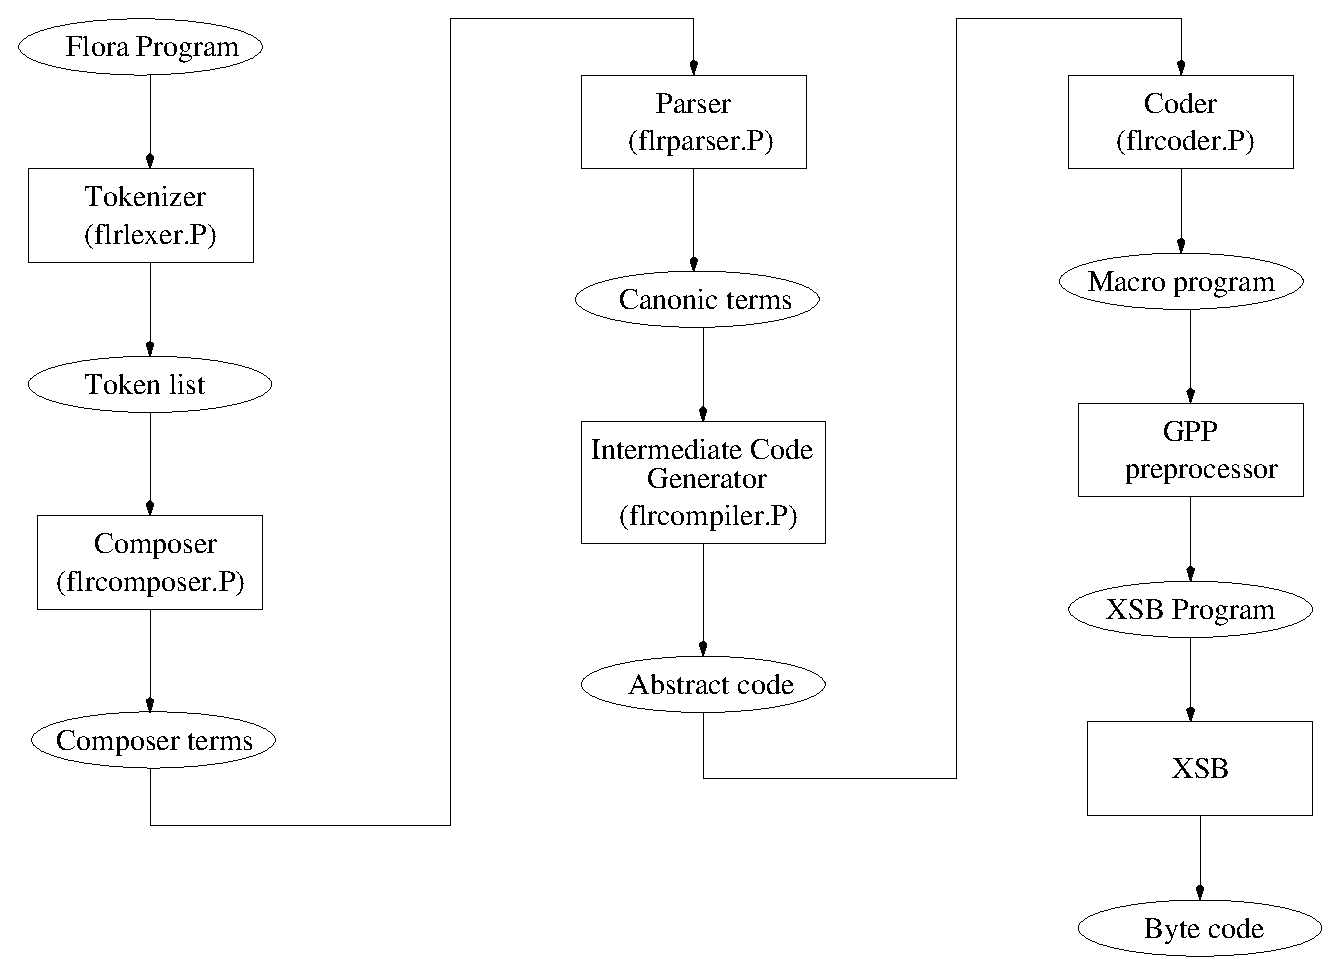
\includegraphics[width=5.5in]{architecture}
  \end{center}
  \caption{The architecture of the \FLSYSTEM system.}
  \label{fig-arch}
\end{figure}
%%

The following is a list of the key files of the system.
%%
\begin{itemize}
\item \texttt{flrshell.P}: The top level module that implements the
  \FLSYSTEM shell --- a subsystem for accepting user commands and queries and
  passing them to the compiler.  See Section~\ref{sec-shell-commands} for a
  full description of shell commands.
\item \texttt{flrlexer.P}: The \FLSYSTEM tokenizer.
\item \texttt{flrcomposer.P}: The \FLSYSTEM composer, which parses tokens
  according to the operator grammar and does other magic.
\item \texttt{flrparser.P}: The \FLSYSTEM parser.
\item \texttt{flrcompiler.P}: The generator of the intermediate code.
\item \texttt{flrcoder.P}: The \FLSYSTEM coder, which generates Prolog code.
\item \texttt{flrutils.P}: Miscellaneous utility predicates for loading
  knowledge bases, checking if files exist, whether they need to be recompiled,
  etc.
\end{itemize}
%%
Additional system libraries are located in the {\tt syslib/} subdirectory.
These include the various printing utilities, implementation for
aggregates, update primitives, and some others. The compiler automatically
determines which of these libraries are needed. When a
library is needed, the compiler generates an {\tt \#include} statement to
include an appropriate file in the {\tt syslibinc} directory. For instance,
to include support for the {\tt avg} aggregate function, the compiler
copies the file {\tt syslibinc/flraggavg\_inc.flh} to the output {\tt .P}
file.  Since {\tt syslibinc/flraggavg\_inc.flh} contains the code to load
the library {\tt syslib/flraggavg.P}, this library will be loaded together
with that output file. The association between the libraries and the files
that need to be included to provide the appropriate functionality is
implemented in the file {\tt flrlibman.P}, which also implements the
utility used to load the libraries.

While {\tt syslib/} directory contains the libraries implemented in Prolog,
the {\tt lib/} directory contains libraries implemented in \FLSYSTEM itself.
Apart from that, the two types of libraries differ in functionality.  The
libraries in {\tt syslib/} implement the primitives that are part of the
syntax of the \FLSYSTEM language itself. In contrast, the libraries in {\tt
  lib/} are utilities that are part of the system, but not part of the
syntax. An example is the pretty-printing library.  Methods and predicates
defined in the libraries in {\tt lib/} are accessible through the {\tt
  @\bs{}libname} system module and (unlike user modules) they are loaded
automatically at startup.

There are several subdirectories that hold the various files that contain
definitions included at compile time. These will be described in a
technical document.

A number of other important directories contain the various included files
(many of which include other files). The directory {\tt flrincludes/}
contains the all-important {\tt flora\_terms.flh} file, which defines all
the names used in the system. These names are defined as preprocessor
macros, so that it would be easy to change them, if necessary.
The directory {\tt genincludes/} currently contains the already mentioned
patch rules. The file {\tt flrpatch.fli} is a template, and {\tt
  flrpatch.flh}, which contains the actual patch rules, is generated from
{\tt flrpatch.fli} during installation.

The directory {\tt includes/} contains (among others) the header file,
which defines a number of important macros ({\it e.g.}, {\tt
  ERGO\_THIS\_WORKSPACE}) that wrap all the names with prefixes to
separate the different modules found in the user knowledge base.  The directory {\tt
  headerinc/} is another place where the template files are located. Each
of these files contains just a few {\tt \#include} statements, mostly for
the files in the {\tt closure/} directory (which, if you recall, contains
pieces of the trailer). All meaningful combinations of these pieces of the
trailer are represented in the file {\tt includes/flrtrailer.flh}.  (Recall
that trailers implement the closure axioms.)

The directory {\tt cc} contains several C programs used by \FLSYSTEM.
Finally, the {\tt
  pkgs/} directory contains a number of \FLSYSTEM packages that are not
core part of the system.

\newpage
\section{Differences Between \FLSYSTEM and the F-logic Syntax}

\FLSYSTEM was developed years after the publication of the initial
works on F-logic \cite{KLW95} and so it benefits from the experience gained
in the use and implementation of the logic. This experience suggested a
number of changes to the syntax (and to some degree also to the
semantics). The main differences are enumerated below.

%%
\begin{enumerate}
\item \FLSYSTEM uses ``,'' to separate methods in F-logic frame formulas. The version of
  the logic in \cite{KLW95} used ``;''. In \FLSYSTEM, ``;'' represents
  disjunction instead. It is also possible to use ``\bs{}and'' instead of ``,''
  and ``\bs{}or'' instead of ``;''.
\item \FLSYSTEM does not use the @-sign to separate method names from their
  arguments. With HiLog extensions the ``@'' sign is redundant.
\item  {\tt p::p} is not a tautology in \FLSYSTEM, i.e., ``::'' is not
  reflexive. This is because our experience showed that the non-reflexive
  use of ``::'' is a more common idiom in knowledge representation.
\item In \cite{KLW95}, types are always inheritable, but values are not.
  In \FLSYSTEM, information about an object
  is strictly separated into information about the object proper
  and information about its superclasses. The latter information is
  \emph{inherited} by the objects. 
  The original F-logic in
  \cite{KLW95} used four types of arrows:
  \texttt{->}, \texttt{->{}>},   {\tt =>} (and {\tt =>{}>}
  because it distinguished
  between functional and set-valued methods), and both were inheritable.
  \FLSYSTEM uses only two types of arrows: \texttt{->} for values and
  \texttt{=>} for types. However, there is now a new type of a formula that
  employs these arrows: \texttt{obj[|meth->val|]}  and
  \texttt{obj[|meth=>type|]}. Here, \texttt{obj} is considered as a class
  and \texttt{obj[|meth->val|]} specifies the default value of the method
  \texttt{meth}, which is inherited by the subclasses and
  members of \texttt{obj}, while \texttt{obj[|meth=>type|]} specifies
  the type of \texttt{meth}, which is also inherited by the subclasses and
  members of the class \texttt{obj}.  

  The semantics of this new type of formulas can be
  characterized by the following logical entailments ($\phi \models \psi$
  means $\phi$ logically entails $\psi$):
  %%
  \begin{quote}
    {\tt X[|M => T|], Y::X $\models$ Y[|M => T|]}\\
    {\tt X[|M => T|], Y:X $\models$ Y[M => T]}
  \end{quote}
  %%
\item Instead of {\tt class[method => \{\}]}
  one should use {\tt class[method => ()]}.
\item Equality (the {\tt :=:} predicate) is implemented only partially in
  \FLSYSTEM. The main limitation is that the congruence axiom for equality
  (``substitution by equals'') works only at the top level and the first
  level of nesting.  For deeper levels of nesting, substitution by equals
  has not been implemented. This is discussed in more detail in
  Section~\ref{sec-eqmaintain}.
\item Behavioral inheritance has a different (and better) semantics in
  \FLSYSTEM compared to \cite{KLW95}.
  This is discussed in Section~\ref{sec-inheritance}.
\item \FLSYSTEM also has many extensions compared to F-logic. First, it
  supports HiLog \cite{hilog-jlp,hilog-icdt-95} and Transaction Logic
  \cite{trans-iclp93,trans-tcs94,trans-chapter-98}.
  Second, it supports a form of defeasible reasoning known as LPDA (logic
  programs with argumentation theories) \cite{lpda-iclp-09}. Third,
  \FLSYSTEM has many syntactic extensions, including full first-order
  formulas that can appear in the rule bodies, many useful builtins, set
  notation, etc.
\end{enumerate}
%%

\newpage

\bibliography{ergo-manual}

\printindex

\end{document}



%%% Local Variables:
%%% mode: latex
%%% TeX-PDF-mode: t
%%% End:
